\chapter{Connections}\label{ch: connections}

Connections are an enormous topic that can be approached from many directions. Their basic practical use is in performing parallel transport and taking derivatives of sections of bundles. However, in geometry and topology they also provide a class of geometric structures that can be used as powerful tools for computing quantities that don't inherently depend on the choice of connection (e.g., certain topological invariants of bundles). Our exposition is based on a combination of \cite{Vakar,RS2,Kolar} but is also, in part, structured with an eye towards the study of $G$-structures and Cartan geometry.

\begin{intu*}
    In \Chap~\ref{ch equivalence problems} we saw how canonical connections arise naturally as the product of Cartan's algorithm for equivalence problems for $G$-structures on manifolds. In particular, the normalization of torsion leads to the $G$-equivariance of any such connection. On abstract principal bundles (as opposed to subbundles of frame bundles, which the definition of a $G$-structure on a manifold), canonical connections do not exist. However, the general definition of principal connections can be seen as a natural consequence of that discussion of integrability, as we will also see at the start of this \chap.
\end{intu*}

\section{General connections}\label{sec general connections}

The Frobenius Theorem~\ref{thm frobenius} states that a distribution $\calH\subset \T M$ is integrable iff it is involutive. However, there is no clear \emph{quantitative measure} of integrability. It turns out that one way to obtain such a quantitative measure is to assume that there is a second distribution, \emph{transverse} to the first one. Namely, let $(\calH,\calV)$ be two distributions on $M$ (subbundles of $\T M$) such that
\[\calH_m\oplus \calV_m=\T_mM \text{ for all }m\in M.\]
This implies that there are globally defined smooth bundle maps (projections), which we denote by the same symbols,
\[\calH:\T M\to \calH,\quad \calV:\T M\to \calV,\quad \calH+\calV=\id_{\T M}.\]
Now we can construct a linear map that measures to what extent $\calH$ fails to be an integrable distribution. Since $\calH$ and $\calV$ are completely interchangeable at this point, we in fact get two maps (the sign choice is conventional):
\begin{align}
    \calR:\fX(M)\times\fX(M)\to \Gamma^\infty(\calV),\quad & \calR(X,Y)=-\calV[\calH X,\calH Y],\\
    \wb{\calR}:\fX(M)\times\fX(M)\to \Gamma^\infty(\calH),\quad & \wb{\calR}(X,Y)=-\calH[\calV X,\calV Y].
\end{align}
Indeed, if $\calR=0$, it means that the Lie bracket of two sections of $\calH$ lies in $\calH$, and therefore $\calH$ is integrable, and similarly $\wb \calR$ detects the integrability of $\calV$. It is obvious that these maps are $C^\infty(M)$-linear and hence are tensors. We call $\calR$ \emph{curvature} and $\wb{\calR}$ \emph{cocurvature}\index{Cocurvature}. Note that the value of $\calR$ depends on the choice of $\calV$, but whether it is zero or not doesn't, so in this sense it's still an objective measure of integrability for $\calH$ (as long as $\calH$ and $\calV$ are everywhere transverse). It turns out that fiber bundles are special in that they come with one canonically defined integrable distribution that we define now. A more sophisticated way of defining the curvature of general connections is as the Fr\"olicher-Nijenhuis bracket $[\calV,\calV]$, see Example~\ref{ex frolicher curvature and torsion}.

\begin{defn}[Vertical bundle]\index{Vertical bundle}
    If $E\overset{\pi}{\to}M$ is a smooth \gls{fb}, then its \emph{vertical subbundle} is the subbundle $\calV E< \T E$ defined as 
    \[\calV E=\ker \pi_\ast\]
    (it is a subbundle by virtue of being the kernel of a bundle morphism). At a point $p\in E$ the fiber is denoted $\calV_pE$. Since each fiber $E_m$, $m\in M$, is an embedded submanifold, and $\calV E$ restricted to $E_m$ coincides with the tangent bundle $\T E_m$ of the fiber, we conclude that $\calV E$ is an integrable distribution. In particular, it is involutive: for any two \emph{vertical vector fields} $X,Y\in \fX_{\mathrm{ver}}(E)\coloneqq\Gamma^\infty(\calV E)$, we have $[X,Y]\in \fX_{\mathrm{ver}}(E)$.
\end{defn}

Therefore cocurvature on fiber bundles always vanishes. Crucially, there is no \emph{natural} ``horizontal'' subbundle $\calH E<\T E$ such that $\calH E\oplus \calV E=\T E$. A connection is, in the broadest sense, a choice of a transverse ``horizontal bundle'' $\calH E$, and its integrability is quantified by the curvature tensor. If it is integrable, then the fiber bundle is not only foliated by its fibers, but also by ``horizontal''  integral submanifolds (locally horizontal sections).

Note that for $m\in M$ and $p\in E$, the sequence
\[0\to \calV_p E=\T_p E_m\overset{\T_p i_m}{\to}\T_p E\overset{\T_p\pi}{\to}\T_mM\to 0\]
is a short exact sequence. Here $m=\pi(p)$ and $E_m\overset{i_m}{\hookrightarrow} E$ is the natural inclusion. This sequence means that we can identify the quotient space $\T_pE\slash \calV_pE$ with $\T_mM$, so we have the following \emph{natural} isomorphism of \glspl{vb} over $E$:
\[\T E\slash \calV E\cong \pi^\ast \T M.\]
A splitting of the above exact sequence is equivalent to choosing a particular subspace $\calH_p E$ in $\T_p E$ complementary to $\calV_p E$ for each $p$, hence specifying a bundle isomorphism between $\pi^\ast \T M$ and the horizontal distribution $\calH E$. But first we will approach this problem from another angle.

As we will see later, determining what the ``horizontal'' directions in a bundle are, in particular, provides one with a \emph{unique} way of lifting paths $\gamma$ in $M$ to paths $\wt\gamma$ in $E$. Doing this for every starting point $p\in E_{\gamma(0)}$, we get a map $E_{\gamma(0)}\to E_{\gamma(1)}$. This map has to be bijective because the lifting clearly respects inverses of paths. Moreover, it will depend only on the \emph{shape} of $\gamma$ and not on how exactly it is parametrized. The next three definitions formalize the concept of \emph{reparametrization invariance} of paths.

\begin{defn}[Sitting instants]\index{Sitting instants}
    A path $\gamma:I\to M$ in a topological space $M$ is said to have sitting instants if there is a neighborhood of the points $0,1$ in $I$ on which $\gamma$ is locally constant.
\end{defn}

\begin{defn}[Thin homotopy]\index{Thin homotopy}
    A thin homotopy between two smooth paths $\gamma_0,\gamma_1:I\to M$ in a smooth manifold $M$ is a smooth homotopy $H:I^2\to M$ between them such that the rank of its derivative $H_\ast:\T(I^2)\to \T M$ is everywhere at most $1$. Equivalently, for any $2$-form $\omega\in\Omega^2(M)$, its pullback must vanish: $H^\ast \omega=0$ on $I^2$.
\end{defn}

\begin{defn}[Path groupoid]\index{Path groupoid}
    The path groupoid $\rmP_1(M)$ of a smooth manifold $M$ is the groupoid whose objects are points of $M$ and morphisms $\mor(p,q)$ are the thin homotopy classes of paths $p\leadsto q$ with sitting instants. Composition of paths is defined via concatenation and reparametrization as usual. The quotient by thin homotopies ensures that this is an associative product with inverses for each path.
\end{defn}

This groupoid can in fact be understood as smooth in a certain sense (it is a ``diffeological groupoid''), but we will not go into those details. We can now define a connection as a prescription (a functor) for taking a path $\gamma$ in $M$ and producing a diffeomorphism $E_{\gamma(0)}\to E_{\gamma(1)}$ in such a way that it is independent of reparametrizations of $\gamma$ and consistent, i.e., functorial w.r.t.\ products of paths. In addition, it needs to depend on $\gamma$ smoothly in a proper sense. Finally, if the bundle carries a $G$-structure, we would like this diffeomorphism to be a morphism of $G$-fibers, i.e., be represented in local frames by actions of elements of $G$ on the typical fiber.

\begin{defn}[Connection I: transport functor]\index{Transport functor}
    Let $(E\overset{\pi}{\to}M,G\acts F,\calG)$ be a $G$-bundle, and more specifically an $\calS$-bundle for some category $\calS$. Let $\calS\mathsf{-Man}^\infty$ be the category of $\calS$-fibers (cf.~Definition~\ref{def S-fibers}). A \emph{transport functor} on $E$ is a functor
    \[\tra: \rmP_1(M)\to \calS\mathsf{-Man}^\infty,\]
    such that for any path $\gamma\in\rmP_1(M)$ the map $\tra_\gamma\coloneqq \tra(\gamma)$ is a morphism (hence isomorphism) of the $G$-fibers over the endpoints:
    \[\tra_\gamma:(E_{\gamma(0)},\calG_{\gamma(0)})\to (E_{\gamma(1)},\calG_{\gamma(1)}),\]
    and which is smooth in the following sense. If $\gamma_t$ is a smooth homotopy of paths in $M$ (not necessarily with fixed ends), then, for any $t\in I=[0,1]$, in some local $\calG$-charts of $E$ at $\gamma_t(0)$ and $\gamma_t(1)$, the representatives of the diffeomorphism $\tra_{\gamma_t}:E_{\gamma_t(0)}\to E_{\gamma_t(1)}$ must depend smoothly on $t$ as elements of $\calS(F,F)$. Since any isomorphism of $G$-fibers is represented by $G$-actions in $G$-frames, this can also be stated as there existing a (finite) collection of $\calG$-charts covering the curves traced out by the endpoints $\gamma_t(0)$ and $\gamma_t(1)$ and a smooth path $g:I\to G$ such that the local representatives of $\tra_{\gamma_t}$ in any of those charts are exactly the action of $g(t)$ on $F$. We will call connections with such parallel transport \emph{$G$-connections}.\index{$G$-connection}

    A \emph{morphism of connections} on $E$ is a natural transformation of two such functors.
\end{defn}

Note that in the case of principal bundles the complicated condition on the values of $\tra$ can be replaced by simply saying that it is a functor into the category $G\mathsf{-Tor}$ of $G$-torsors. This definition can be made significantly neater by introducing a few extra functors, but we direct the reader to \cite{schreiber} for that.

\begin{defn}[Flat connection]\index{Connection!Flat}
    A connection defined via a transport functor $\tra$ on a bundle $E$ is called flat if for any path $\gamma$ in $M$, the map $\tra_\gamma$ is invariant under homotopies of $\gamma$ with fixed endpoints.
\end{defn}


\begin{example}[Absolute parallelism]
    Recall from Definition~\ref{def parallelizable} that if $E\to M$ is a trivial \gls{fb}, then a particular choice of a global trivialization $\chi:E\to M\times F$ is called an \emph{absolute parallelism}\index{Parallelism!Absolute}. Each absolute parallelism naturally determines a unique flat connection. Namely, the parallel transport operator (independent of the path) from fiber $E_m$ to fiber $E_{m'}$ maps $\chi^{-1}(m,f)$ to $\chi^{-1}(m,f')$.
\end{example}

\begin{example}[Canonical flat connections on a Lie group]\label{ex flat connections on G}
    If $G$ is a Lie group, then the tangent bundle $\T G$ admits two obvious flat connections. The first, called the $(-)$-connection, has parallel transport acting by left translations, i.e., $\T_g G$ is mapped to $\T_h G$ by $\rmL_{hg^{-1}\ast}$. The second, so called $(+)$-connection, has parallel transport given by $\rmR_{g^{-1}h\ast}$, instead. Since these transports are independent of the path, these connections are flat. Both of them derive from absolute parallelisms $\T G\to G\times\frakg$ given by the left and right Maurer-Cartan forms, respectively.
\end{example}



\begin{prop}
    A bundle is flat iff it admits a flat connection.
\end{prop}
\begin{proof}
    By Definition~\ref{def flat G-bundle}, a bundle is flat if it  has a $G$-atlas with locally constant transition functions. Then a path $\gamma$ in the base can be turned into a ``horizontal'' path $t\mapsto (\gamma(t),f_\alpha)$ in each local chart $U_\alpha\times F$ overlapping with the image of $\gamma$. The points $f_\alpha$ are chosen so that $f_\beta=g_{\beta\alpha}\cdot f_\alpha$, where $g_{\alpha\beta}\in G$ is the constant transition function on $U_{\alpha\beta}$. This produces a consistently defined path in the bundle because transition functions are constant. By applying this to every starting point, we get a transport map which obviously depends only on the endpoints of $\gamma$, thus defining a flat connection.

    Conversely, given a flat connection $\tra$, we can cover the base manifold with contractible open sets $U_\alpha$, pick a basepoint $x_\alpha$ in each, and use parallel transport along arbitrary paths $x_\alpha\leadsto y_\alpha$ inside $U_\alpha$ to obtain diffeomorphisms $\varphi_{\alpha,y_\alpha}:E_{y_\alpha}\to E_{x_\alpha}$ for all $y_\alpha\in U_\alpha$. Due to flatness these diffeomorphisms depend only on $y_\alpha$. Hence we can define a map $\pi^{-1}(U_\alpha)\to U_\alpha\times E_{x_\alpha}$ by $\chi_\alpha(p)=(\pi(p),\varphi_{\alpha,\pi(p)}(p))$. Further we can choose arbitrary diffeomorphisms compatible with the $G$-structure of the bundle between each $E_{x_\alpha}$ and the typical fiber $F$. This allows us to treat the $\chi_\alpha$ as local trivializations. The transition functions between them are constant because they can be written in terms of these fixed diffeomorphisms and the transport diffeomorphisms $E_{x_\alpha}\to E_{x_\beta}$, which are entirely independent of any other points in the base.
\end{proof}

An obvious consequence of the definition of parallel transport is that it endows the bundle with \emph{unique horizontal path liftings}: given a path $\gamma:I\to M$ and a point $p\in\pi^{-1}(\gamma(0))$, its horizontal lifting is the smooth path $\wt{\gamma}(t)=\tra_{\restr{\gamma}{[0,t]}}(p)$. By doing this for all paths through $m\in M$ and all $p\in E_m$, each parallel transport functor induces a distribution $\calH E<\T E$ consisting of ``horizontal'' vectors. This leads to our second definition of a connection (as we will see, it is a bit more general than Definition I).


\begin{defn}[Connection II: general connection]\index{Connection!General}
    Given a $G$-bundle $(\tuple{E\overset{\pi}{\to}M,G\acts F,\calG})$, an general connection on it is a smooth vector subbundle $\calH E<\T E$ such that $\calH E\oplus \calV E=\T E$. The decomposition $\T_pE=\calH_pE\oplus \calV_pE$ induces the natural projections which we denote by two pairs of symbols:
    \[\T_pE\to \calH_pE\oplus \calV_pE,\quad X_p\mapsto (\hor X_p,\ver X_p).\]
    For any smooth vector field $X\in\fX(E)$, the assignments $p\mapsto \hor X_p$ and $p\mapsto \ver X_p$ are also smooth vector fields, denoted $\hor X$ and $\ver X$, respectively.

    The connection $\calH E$ is called \emph{flat} if it is integrable as a distribution (or, equivalently, by the Frobenius Theorem, if it is involutive).
\end{defn}


\begin{rem}[Connections via jet bundles]\label{rem connections via jets}
    Recall from \S\ref{sec: jets and cartan distr} that a $1$-jet $p'\in \rmJ^1 E$ with $\pi^1_0(p')=p\in E$ is naturally identified with an R-plane $L_{p'}<\T_p E$. R-planes are exactly the possible choices of horizontal subspaces at $p$. Thus, a general connection on $E$ can be identified with a smooth section $\varGamma$ of the \emph{affine} bundle $\pi^1_0:\rmJ^1 E\to E$, and vice versa. This affine bundle is modeled on the \gls{vb} $\pi^\ast(\T^\ast M)\otimes_M \calV E\to E$. If $E$ has local coordinates $(\tuple{x^1,\ldots,x^n,u^1,\ldots,u^k})$ generating canonical fiber coordinates $p^a_i$ on the fibers of $\pi^1_0$, then $\varGamma$ is locally represented by functions $\varGamma^a_i$, $i=1,\ldots,n$, $a=1,\ldots,k$. Under a fiber-preserving change of coordinates $(\bf{x},\bf{u})\mapsto (\bar{\bf{x}},\bar{\bf{u}})$, the components of $\varGamma$ transform according to 
    \[\wb{\varGamma}^a_i=\frac{\partial x^j}{\partial \wb{x}^i}(\partial_{x^j}+\varGamma^b_j\partial_{u^b})\wb{u}^a.\]
\end{rem}

One thing to note immediately is that the map $X\mapsto \ver X$ is  $C^\infty(E)$-linear and can therefore be identified with a $\calV E$-valued $1$-form on $E$. We denote it by $\calV\in\Omega^1(E;\calV E)$. We have $\calH E=\ker \calV$. This leads to the third definition:

\begin{defn}[Connection III: general connection]
    Given a \gls{fb} $E\overset{\pi}{\to}M$, a general connection on it is a smooth $1$-form $\calV\in\Omega^1(E;\calV E)$ with values in the vertical bundle of $E$ such that $\calV\circ\calV=\calV$ and $\im\calV=\calV E$ (so that it is a projection $\T E\to \calV E$). Given a general connection, we define the vertical and horizontal parts of a vector via
    \[\ver X=\calV(X),\quad \hor X=X-\calV(X).\]
\end{defn}

\begin{rem}[\ref{rem connections via jets} continued]\label{rem connections via jets 2}
    In terms of the section $\varGamma$ of the affine jet bundle $\rmJ^1 E\to E$, the vertical projection operator $\calV$ is given by 
    \[\calV=\theta^{(1)}\circ\varGamma,\]
    where $\theta^{(1)}$ is the canonical contact form $\theta^a=\dd u^a-p^a_i\dd x^i$ on $\rmJ^1 E$ extended to an embedding $\theta^{(1)}:\rmJ^1 E\to \T^\ast E\otimes_E \calV E$ given in local coordinates $(\tuple{x^i,u^a,p^a_i})$ by 
    \[\theta^{(1)}=\theta^a\otimes \partial_{u^a}:\quad \rmJ^1 E\hookrightarrow \T^\ast E\otimes_E \calV E.\] 
    Thus, locally we have 
    \[\calV=(\dd u^a-\varGamma^a_i\dd x^i)\otimes \partial_{u^a}:\quad X^i\partial_{x^i}+X^a\partial_{u^a}\mapsto (X^a-\varGamma^a_i X^i)\partial_{u^a}.\]
\end{rem}

\begin{rem}
    Crucially, at this point we are not able to take exterior derivatives of connection forms, since they take values in a vector bundle $\calV E$, and not a vector space. This situation will be remedied on principal bundles, whose vertical bundle is trivial and has a canonical trivialization (the Maurer-Cartan form).
\end{rem}

\begin{xca}
    Show that definitions II and III are equivalent, i.e., there is a one-to-one correspondence between subbundles $\calH E$ and $1$-forms $\calV$.
\end{xca}


\begin{prop}
    Let $\calV$ be a connection on $E\overset{\pi}{\to}M$. For any two horizontal vector fields $X,Y\in\Gamma^\infty(\calH E)$, their ``Lie bracket up to $\calH E$'', i.e., the value of $([X,Y]\mod \calH E)\in \Gamma^\infty(\T E\slash \calH E)$ at a point $p\in E$, is $C^\infty(E)$-linear. In particular, the question of involutivity can be answered pointwise.
\end{prop}
\begin{proof}
    Let $\alpha\in\Omega^1(E)$. The chain rule and Cartan's formula imply
    \[i_{[X,Y]}\alpha=\Lie_Xi_Y \alpha-i_Y \Lie_X\alpha=\Lie_Xi_Y\alpha-i_Y(\dd (i_X\alpha))-i_Yi_X\dd\alpha.\]
    Suppose that for an open $U\subset E$ containing $p\in E$, we can find $\alpha_i\in\Omega^1(\restr{E}{U})$, $1\leq i\leq l$, such that $\restr{\calH E}{U}=\bigcap_i\ker\alpha_i$. Then the fact that $X,Y\subset \calH E$ implies that $i_X\alpha_i=0$, so
    \[\alpha_i([X,Y])=-\dd\alpha_i(X,Y).\]
    The value of the right hand side is $C^\infty(E)$-linear in $X$ and $Y$, and the left hand side uniquely determines $[X,Y]\mod \calH E$, since $\restr{\calH E}{U}=\bigcap_i \ker\alpha_i$. 

    What remains to show is that such $\alpha_i$ can indeed be chosen. Let $\pi':\calV E\to E$ denote the induced projection and let $\chi:\pi^{\prime-1}(U)\to U\times\bbR^k$ be a local trivialization. We let $U$ shrink around $p$ until it is contained in a chart $\kappa:U\to \bbR^n$. Then the components $\{\alpha_i\}_{i=1}^{n+k=l}$ of the map
    \[\T E\supset (\pi'\circ\calV)^{-1}(U)\overset{\alpha\coloneqq (\kappa\times\id_{\bbR^k})\circ\chi\circ \calV}{\longrightarrow}\kappa(U)\times\bbR^k\subset \bbR^{n+k},\]
    where we view the connection form as a map $\calV:\T E\to \calV E$, are precisely what we are looking for.
\end{proof}

We have thus identified the following \emph{tensor field} that quantifies the obstruction to the integrability of the horizontal distribution $\calH E$.

\begin{defn}[General curvature form]\index{Curvature!General}
    Given a general connection $\calV$ on a bundle $E$, the general curvature $2$-form $\calR\in \Omega^2(E;\calV E)$ is defined by
    \[\calR(X,Y)\coloneqq -\calV([\hor X,\hor Y])=-\calV([X-\calV(X),Y-\calV(Y)]).\]
    Its value is the unique representative of $[\hor X,\hor Y]\mod \calH E$ that lies in $\ker(\hor)$. The general connection $\calV$ is called \emph{flat} if $\calR\equiv 0$.
\end{defn}


\begin{xca}
    Show that flatness (integrability) of $\calH E$ is equivalent to flatness of $\calV$ and the existence of a flat general connection is equivalent to the flatness of the bundle $E$.
\end{xca}

It follows from the definition of a connection that the restriction of $\pi_{\ast p}$ to $\calH_pE$ defines a linear isomorphism to $\T_{\pi(p)}M$.
This allows us to lift a vector $X_m\in \T_{\pi(p)}M$, $m=\pi(p)$, to a unique horizontal vector $X_p^h\in \calH_pE$. Applying this pointwise to a vector field $X\in\fX(M)$, we construct the \emph{horizontal lift} $X^h:E\to \calH E\subset \T E$. This is again a smooth vector field since it can be written as the composition
\[E\overset{\id_E\times \pi_{\T M}}{\longrightarrow}E\times M \overset{\id_E\times X}{\longrightarrow}\pi^\ast \T M \overset{i}{\longrightarrow}\calH E\subset \T E,\]
where $i$ is the inclusion, we understand the pullback bundle $\pi^\ast \T M$ to be embedded in $E\times \T M$, and where $\pi_{\T M}:\T M\to M$ is the bundle projection.

\begin{rem}[\ref{rem connections via jets 2} continued]\label{rem connections via jets 3}
    Returning to the description of the connection as a section $\varGamma$ of the affine jet bundle $\rmJ^1 E\to E$, the horizontal lift operator can be written in terms of the canonical lifting $\partial_{x^i}\mapsto D_i$, where $D_i$ is the total derivative operator. This mapping lifts a tangent vector of $M$ to any point above it in $\rmJ^1 E$ and allows us to define the canonical embedding 
    \begin{align}
        \lambda^{(1)}=\dd x^i\otimes D_i:\rmJ^1 E&\hookrightarrow (\pi^\ast\T^\ast) M\otimes_E \T E,\\ 
        (x^i,u^a,p^a_i)&\mapsto \dd x^i\otimes (\partial_{x^i}+p^a_i\partial_{u^a}).
    \end{align}
    Then the horizontal lift operator is given by
    \[\lambda^{(1)}\circ\varGamma=\dd x^i\otimes(\partial_{x^i}+\varGamma^a_i\partial_{u^a}):\quad X^i\partial_{x^i}\mapsto X^i(\partial_{x^i}+\varGamma^a_i\partial_{u^a}).\]
    For more details on this approach to connections, see \cite{Giachetta}.
\end{rem}

How are the flows of $X$ and $X^h$ related? If $\gamma$ is an integral curve of $X^h$, then $\pi\circ\gamma$ is clearly an integral curve of $X$, so we see that 
\[\pi\circ F^{X^h}_t=F^{X}_t\circ \pi.\]
Therefore, for any two $X,Y\in \fX(M)$:
\[\pi_{\ast p}([X^h,Y^h](p))=[X,Y](\pi(p)),\]
and we conclude
\[\calR(X^h,Y^h)=-\calV([X^h,Y^h])=[X,Y]^h-[X^h,Y^h].\]
We have proven the following.

\begin{cor}\label{cor curvature in terms of hor}
    Using the identification $\pi^\ast \T M\overset{i}{\cong}\calH E\subset \T E$, we can view $\calR$ as a map $\pi^\ast\left(\bigwedge\nolimits^2\T M\right)\to \calV E$ given by 
    \[(X_m,Y_m,p)\mapsto (X,Y,p)\mapsto [X^h,Y^h](p)-[X,Y]^h(p),\]
    where $X,Y\in \fX(M)$ are arbitrary vector fields on $M$ such that $X(m)=X_m$ and $Y(m)=Y_m$, and $m=\pi(p)$.
\end{cor}

Let us now take a look at the local representatives of the connection form. Let $(U_\alpha,\chi_\alpha)$ be a local trivialization of our bundle $E\overset{\pi}{\to}M$ around a point $p\in E$, and let $F$ be the typical fiber. Then in this trivialization
\begin{multline}
    (\chi_\alpha)_\ast(\restr{\calH E}{U_\alpha})=(\chi_\alpha)_\ast\circ i(\pi^\ast (\restr{\T M}{U_\alpha}))=\{(\chi_\alpha)_\ast\circ i(X,p)\mid \pi_{\T M}(X)=\pi(p)\}=\\
    =\{(X,-\varGamma^\alpha(X,f))\in \T U_\alpha\times \T F\mid (X,f)\in \restr{\T M}{U_\alpha}\times F\}
\end{multline}
for some smooth map $\varGamma^\alpha:\restr{\T M}{U_\alpha}\times F\to \T F$ known as the \emph{Christoffel form}\index{Christoffel form} for this trivialization. More explicitly,
\[\varGamma^\alpha(X,f)=\pr_2\circ (\chi_\alpha)_\ast\circ \calV\circ (\chi_\alpha)_\ast^{-1}(X,0),\]
where $\pr_2:\T U_\alpha\times \T F\to \T F$ is the projection onto the second component and $0 \in \T_fF$. Then the projection $\calV:\T E\to \calV E$ is locally represented as follows:
\[\wh{\calV}_\alpha=(\chi_\alpha)_\ast\circ \calV\circ (\chi_\alpha)_\ast^{-1}(X,\xi)=\xi+\varGamma^\alpha(X,\pi_{\T F}(\xi)),\quad (X,\xi)\in \T U_\alpha\times \T F.\]

Finally, it is essential to discuss how connections interact with pullbacks of bundles. Recall that categorical pullbacks of smooth fiber bundles exist due to the fact that a fiber bundle is a submersion, and a submersion is transversal to any smooth map (since the topological pullback of a pair of transversal maps $(f,\pi):N\times E\to M$ is a smooth submanifold of $N\times E$).

\begin{prop}[Pullback connection {{\cite[1.2.7]{Vakar}}}]\index{Connection!Pullback}
   Let $E\overset{\pi}{\to}M$ be a \gls{fb} and $f:N\to M$ a smooth map. Let $\pi':f^\ast E\to M$ be the pullback bundle and let $\wt f:f^\ast E\to E$ be its other natural projection. Let $E$ be equipped with a general connection $\calV$. Then the pullback induces a unique connection denoted (confusingly) $f^\ast\calV$ on $f^\ast E$ such that $\wt{f}_\ast\circ (f^\ast \calV)=\calV\circ {\wt f}_\ast$.
\end{prop}
\begin{proof}
    First, why is $f^\ast\calV$ a connection, i.e., a projection $\T(f^\ast E)\to \calV(f^\ast E)$? The main observation is that $\T_q{\wt f}$ restricts to a linear isomorphism 
    \[\calV_q (f^\ast E)=\T_q((f^\ast E)_{\pi'(q)})\to \T_{\wt{f}(q)}(E_{\pi(\wt{f}(q))})=\calV_{\wt{f}(q)}E.\]
    Indeed, $\wt f$ is a diffeomorphism of fibers $(f^\ast E)_{\pi'(q)}\to E_{\pi(\wt{f}(q))}$. This means that the following commuting square uniquely defines $f^\ast\calV$:
    \[(\calV)_{\wt{f}(q)}\circ \wt{f}_{\ast q}=\wt{f}_{\ast q}\circ (f^\ast \calV)_q.\]
    Finally, note that $\wt{f}_{\ast q}\circ (f^\ast\calV)^2_q=\calV_{\wt{f}(q)}\circ \wt{f}_{\ast q}\circ (f^\ast\calV)_q=(\calV)^2_{\wt{f}(q)}\circ \wt{f}_{\ast q}=(\calV)_{\wt{f}(q)}\circ \wt{f}_{\ast q}=\wt{f}_{\ast q}\circ (f^\ast \calV)_q$, and therefore, since $\wt{f}_{\ast q}$ is an isomorphism, $(f^\ast\calV)^2=f^\ast\calV$.
\end{proof}

\begin{rem}
    Given two fiber bundles $E_1,E_2$ over $M$ with fiber product $E_1\overset{\pi^1}{\leftarrow}E_1\times_M E_2\overset{\pi^2}{\to}E_2$, and respective connections $\calV_1$ and $\calV_2$ on them, we can construct a connection $\calV_1\times_V\calV_2\coloneqq \calV=\pi^{1\ast}\calV_1+\pi^{2\ast}\calV_2$ on $E_1\times_M E_2$, called the \emph{product connection}.
\end{rem}


Finally, let us connect general connections to parallel transport, since that is the most intuitive (and, in a way, ``correct'') way of defining a connection. We have seen that each tangent vector on $M$ has a unique horizontal lift $X^h$ under a given general connection. Therefore we can attempt to lift entire curves $\gamma:I\to M$ by lifting each velocity vector $\dot\gamma(t)$ individually and solving the resulting differential equation.


We now examine to what extent a connection $\calV$ determines parallel transports.

\begin{thm}[Parallel transport]\label{prop parallel tra}\index{Parallel transport}
    Let $\calH E$ be a general connection on a fiber bundle $E\overset{\pi}{\to}M$ and let $\gamma:(a,b)\to M$ be a smooth path with $0\in(a,b)$. Then there exists an open neighborhood $\calD_\gamma\in E\times I$ of $E_{\gamma(0)}\times\{0\}$ and a smooth map $T_\gamma:\calD_\gamma\to E$ such that for all $(p,t)\in \calD_\gamma$: 
    \begin{enumerate}[label=(\arabic*)]
        \item $\pi(T_\gamma(p,t)=\gamma(t)$;
        \item $\frac{\dd}{\dd t}T_\gamma(p,t)\in \calH E$;
        \item $T$ is reparametrization invariant: if $\phi:(a',b')\to (a,b)$ is smooth with $0\in(a',b')$, then for all $s\in (a',b')$, 
        \[T_\gamma(p,\phi(s))=T_{\gamma\circ\phi}(T_\gamma(p,\phi(0)),s).\]
    \end{enumerate}
\end{thm}
\begin{proof}
    The standard proof is the following. Let $F$ be the typical fiber and let $\chi_\alpha:\pi^{-1}(U_\alpha)\to U_\alpha\times F$ be a local trivialization for $E$ around $\gamma(0)$. Property (2) can equivalently be states as demanding that $\calV(\frac{\dd}{\dd t}T_\gamma(p,t))=0$. In the local chart this condition becomes
    \[\frac{\dd}{\dd t}\Phi_\gamma(p',t)=-\varGamma^\alpha\left(\dot\gamma(t),\Phi_\gamma(p',t)\right),\]
    where $\Phi_\gamma(p',t)=\pr_2\circ \chi_\alpha\circ T_\gamma(\chi_\alpha^{-1}(p'),t)\in F$. Now, the right hand side of this equation is a smooth time-dependent vector field, therefore from general theory of ODE's this equation has a unique maximal integral solution $\Phi_\gamma:U_\gamma'\to U_\alpha\times F$ on some open domain $D_\gamma'\subset U_\alpha\times F\times I$. Since $\chi_\alpha$ is a diffeomorphism, we obtain a map $T_\gamma:\calD_\gamma\to E$ by $T_\gamma(p,t)=\chi_\alpha^{-1}(\gamma(t),\Phi_\gamma(\chi_\alpha(p),t))$.

    Property (3) is also easily checked. Indeed, write $\gamma^h(t)\coloneqq T_\gamma(p,t)$ for a horizontal lift of $\gamma$. Then $\frac{\dd}{\dd s}(\gamma^h\circ \phi(s))=\dot\phi(s)\cdot \gamma^{h\prime}(\phi(s))$, and $\pi\circ\gamma^h\circ\phi=\gamma\circ\phi$, so $\gamma^h\circ\phi$ is a horizontal lift of $\gamma\circ\phi$. Finally, $\gamma^h\circ\phi(0)=T_\gamma(p,\phi(0))$, so the conclusion follows from uniqueness.
\end{proof}


For this to extend to a proper parallel transport functor, we need to be able to lift paths globally. This leads us to the following definition.

\begin{defn}[Connection IV: Ehresmann connection]\index{Connection!Ehresmann}
    A general connection $\calH E$ on a bundle $E\overset{\pi}{\to}M$ is called an Ehresmann connection if it is \emph{complete} in the sense that the parallel transport $T_\gamma$ for any smooth curve $\gamma:(a,b)\to M$ (with $0\in (a,b)$) is defined on all of $E_{\gamma(0)}\times (a,b)$. 
\end{defn}
We provide the following theorem without proof.
\begin{thm}[{{\cite{Hoyo}}}]
    Every \gls{fb} admits a complete connection.
\end{thm}

Note that the vertical bundle $\calV E$, and hence the concept of general a connection $\calH E$, is well-defined on all surjective submersions $\pi:E\to M$. Then the following generalization of Ehresmann's Fibration Theorem~\ref{thm Ehresmann} is easily established.
\begin{thm}[Ehresmann]\index{Theorem!Ehresmann}
    A surjective submersion $\pi:E\to M$ is a locally trivial fibration iff  each $m\in M$ admits a neighborhood $U\subset M$ and a connection $\calH E$ that is complete whence restricted to $U$.
\end{thm}
\begin{proof}
    We can simply repeat the proof given in \S\ref{proof of Ehresmann thm}, but this time letting $X_i$ be the unique horizontal lifts of $\partial_i$ to the entire trivial pieces $\pi^{-1}(U)$.
\end{proof}

\begin{example}
    Every general connection on a bundle with compact fibers is complete. 
\end{example}


\begin{xca}
    Show that definitions I and IV are equivalent, i.e., there is a one-to-one correspondence between Ehresmann connections and smooth parallel transport functors.
\end{xca}


Note that parallel transport only requires the path $\gamma$ to be $C^1$-differentiable. Let $C(m)$ be the group of piecewise smooth loops starting and ending at $m\in M$. The parallel transport along $\gamma\in C(m)$ yields an automorphism of the fiber $E_m$. For the trivial curve it coincides with identity. Assuming the parallel transport respects the structure group, the resulting map $C(m)\to G$ is called the \emph{holonomy representation}. The image of this homomorphism forms a subgroup of the structure group. Further, let $C^0(m)\subset C(m)$ be the subgroup of nullhomotopic closed curves.

\begin{defn}[Holonomy group]\index{Holonomy group}\index{Holonomy group!Restricted}
    Given an Ehresmann connection $\calH E$ on $E\overset{\pi}{\to}M$, the group of parallel transports along elements of $C(m)$ is called the holonomy group  with basepoint $m$. It will be denoted $\Hol_m(\calH E)$. The \emph{restricted holonomy group} is the subgroup $\Hol^0_m(\calH E)<\Hol_m(\calH E)$ generated by parallel transports along elements of $C^0(m)$.
\end{defn}

\begin{defn}[Monodromy of flat connections]\index{Monodromy!of a flat connection}
    In the special case that $\calH E$ is flat (integrable), parallel transport is homotopy-invariant, and then we also get a representation of the fundamental group $\pi_1(M,m)\to G$ called the \emph{monodromy representation}. Its image is the \emph{monodromy group}, denoted $\Mon_m(\calH E)$.
\end{defn}

Regardless of whether a connection is complete, we can always expect parallel transport to be possible for loops contained in a sufficiently small neighborhood in the base, and a fixed initial condition $p\in E$. This allows us to describe curvature in terms of \emph{infinitesimal holonomy}.

\begin{prop}[Curvature as infinitesimal holonomy]
    Let $E\overset{\pi}{\to}M$ be a \gls{fb} and $\calH E$ a connection with curvature form $\calR\in\Omega^2(E;\calV E)$. If $X,Y\in\fX(M)$ are two commuting vector fields, $[X,Y]=0$, then 
    \[\calR(X,Y)(p)=\restr{\frac{\dd^2}{\dd t\dd s}\left(
    F^{X^h}_{-t}\circ F^{Y^h}_{-s}\circ F^{X^h}_t\circ F^{Y^h}_s(p)
    \right)}{t=s=0}\]
\end{prop}
\begin{proof}
    Using Corollary~\ref{cor curvature in terms of hor}, combined with $[X,Y]=0$, we have 
    \[\calR(X,Y)(p)=-[X^h,Y^h](p).\] 
    The claim then follows from the well-known identity \eqref{eq Lie bracket in terms of flows} for the Lie bracket of vector fields in terms of their flows.
\end{proof}
\begin{cor}
    A general connection is flat iff all of its restricted holonomy groups are trivial.
\end{cor}

\begin{rem}
    Note that definitions II, III, and IV, of general connections fail to incorporate any $G$-structure that $E$ might carry. The easiest workaround is to say that a general connection is \emph{compatible} with a given $G$-structure iff all parallel transport operators induced by it are isomorphisms of $G$-fibers. Clearly, this is an extremely indirect way of defining compatibility. The standard solution to this issue, and the one we shall follow below, is to first define compatible connections on \emph{principal} bundles, where it is easy, and then use them to \emph{induce} compatible connections on associated bundles.
\end{rem}







\section{Horizontal forms}

Before we discuss connections on principal bundles, it will be useful to introduce the concept of horizontal differential forms. The following discussion is independent of any choice of connection and relies only on the vertical bundle.

\begin{defn}[Horizontal forms]\index{Horizontal form}
    Let $(P\to M,G\overset{\Phi}{\acts} P)$ be a (right) principal bundle and let $G\overset{\sigma}{\acts}V$ be a finite-dimensional representation of $G$ whose values we denote by $G\ni g\mapsto \sigma_g\in \GL(V)$. A $V$-valued differential $k$-form $\wt\eta\in\Omega^k(P;V)$ is called \emph{horizontal, or strongly semibasic, of type $\sigma$} if
    \begin{enumerate}
        \item $\restr{\wt\eta}{\calV P}=0$, i.e., it is annihilated by any vertical vector (always true for $k=0$);
        \item $\Phi_g^\ast \wt\eta=\sigma_{g^{-1}}\circ\wt\sigma$ for every $g\in G$ (for a left principal bundle replace $\sigma_{g^{-1}}$ with $\sigma_g$).
    \end{enumerate}
    The vector space of horizontal $k$-forms of type $\sigma$ is denoted by $\Omega^k_{\hor}(P;V)^\sigma$. Correspondingly, the space of ordinary horizontal $k$-forms is denoted $\Omega^k_{\hor}(P)$. 
\end{defn}


\begin{rem}
    \begin{enumerate}
        \item Despite the name, the definition of horizontal forms does not depend on any choice of the horizontal distribution. For this reason, horizontal forms are also sometimes called \emph{strongly semibasic}. The difference between semibasic and strongly semibasic forms is that the kernel of the latter is \emph{exactly} the vertical bundle, and not more.\index{Semibasic form}
        \item Differential forms on a \gls{fb} $E\overset{\pi}{\to} M$ that have the form $\pi^\ast\omega $ for some $\omega\in \Omega^{\smbullet}(M)$ are called \emph{basic}.\index{Basic form}
        \item If $x^1,\ldots,x^n,y^1,\ldots,y^r$ are local coordinates on the bundle $E\to M$ such that $x^1,\ldots,x^n$ project to form local coordinates on $M$, then every semibasic form can be written as $a_I(\bf{x},\bf{y})\dd \bf{x}^I$, where $I=(i_1,\ldots,i_p)$ is a multi-index, so $\dd \bf{x}^I=\dd x^{i_1}\wedge\cdots\wedge\dd x^{i_p}$. Meanwhile, a local basis for basic forms is of the form $a_I(\bf{x})\dd \bf{x}^I$.
    \end{enumerate}
\end{rem}

Now consider the associated bundle $E\coloneqq P^{[\sigma]}=P\times^G V$.

\begin{prop}[{{\cite[Prop.~1.2.12]{RS2}}}]\label{prop 1.2.12 RS2}
    To every element $\wt{\eta}\in \Omega^k_{\hor}(P;V)^\sigma$ there corresponds a unique element $\eta\in \Omega^k(M;E)$ such that the following diagram commutes
    \[\begin{tikzcd}
        \bigwedge\nolimits^k P\arrow[r,"\pr\times\wt\eta"] \arrow[d,"\bigwedge\nolimits^k \pi_\ast",swap]& P\times V\arrow[d,"\iota"]\\
        \bigwedge\nolimits^kM\arrow[r,"\eta"] & E,
    \end{tikzcd}\]
    where $\pr:\bigwedge\nolimits^k P\to P$ denotes the natural projection. The assignment $\wt\eta\mapsto \eta$ defines a vector space isomorphism $\Omega^k_{\hor}(P;V)^\sigma\to \Omega^k(M;E)$.
\end{prop}
\begin{proof}
    Let $m\in M$ and $X_i\in T_mM$, $i=1,\ldots,k$. Choose $p\in P$ fulfilling $\pi(p)=m$ and $Y_i\in T_pP$ such that $\pi_\ast (Y_i)=X_i$. We define
    \[\eta_m(X_1,\ldots,X_k)\coloneqq \iota_p\circ \wt\eta_p(Y_1,\ldots,Y_k).\label{eq 1.2.13 RS2}\]
    We must show that this definition does neither depend on the choice of $p$ nor on the choice of the $Y_i$. Thus, take $p'=\Phi_g(p)$ and tangent vectors $Y_i'$ at $p'$ which also project onto the $X_i$. Then, there exist vertical vectors $Z_i\in \T_{p'}P$ such that $Y_i'=\Phi_{g\ast}(Y_i)+Z_i$ and we obtain
    \begin{multline}
        \iota_{p'}\circ\wt\eta_{p'}(Y_1',\ldots,Y_k')=\iota_{p\cdot g}\circ \wt\eta_{p\cdot g}(\Phi_{g\ast}(Y_1)+Z_1,\ldots,\Phi_{g\ast}(Y_k)+Z_k)=\\
        =\iota_p\circ \sigma_g\circ (\Phi_g^\ast \wt\eta)_p(Y_1,\ldots,Y_k)=\iota_p\circ \wt\eta_p(Y_1,\ldots,Y_k).
    \end{multline}
    Here, we have used $\iota_{p\cdot g}=\iota_p\circ \sigma_g$ together with the horizontality and equivariance of $\wt\eta$. Bijectivity and linearity of the assignment $\wt\eta\mapsto \eta$ follows from the bijectivity and linearity of $\iota_p$.
\end{proof}

Note that, conversely, we have
\[\wt{\eta}_p=\iota_p^{-1}\circ (\pi^\ast\eta)_p.\label{eq 1.2.14 RS2}\]

\begin{rem}\label{rem 1.2.13 RS2}
    Note that elements $\wt\eta\in\Omega^{\smbullet }_{\hor}(P;V)^\sigma$ and $\eta\in \Omega^{\smbullet }(M;E)$ have a well-defined wedge product with any regular form $\beta\in \Omega^{\smbullet }(M)$ on $M$, since $\wt{\beta}\wedge \wt\eta=\widetilde{\beta\wedge\eta}$. Thus both of these spaces are $\Omega^{\smbullet }(M)$-modules.
\end{rem}

Let us also study local representations of horizontal forms. Let $(U_\alpha,\chi_\alpha)$ be a local trivialization of $P$, let $\wt{s}_\alpha:\restr{P}{U_\alpha}\to G$ be the corresponding equivariant map and let $s_\alpha:U\to P$ be the corresponding local section. We define the local representative of $\wt\eta\in\Omega^k_{\hor}(P;V)^\sigma$ by
\[{\wt\eta}_\alpha\coloneqq s_\alpha^\ast\wt\eta.\label{eq 1.2.15 RS2}\]
This is a $V$-valued  $k$-form on $U$. The following proposition shows that a horizontal form of type $\sigma$ may be reconstructed from its local representatives.

\begin{prop}[{{\cite[Prop.~1.2.14]{RS2}}}]
    Let $\wt\eta\in \Omega^k_{\hor}(P;V)^\sigma$ and let $\wt{\eta}_\alpha$ be its representative in a local trivialization $(U_\alpha,\chi_\alpha)$ given by \eqref{eq 1.2.15 RS2}. Then, for every $p\in \restr{P}{U_\alpha}$, we have
    \[\wt{\eta}_p=\sigma_{\wt{s}_\alpha(p)^{-1}}\circ (\pi^\ast \wt{\eta}_\alpha)_p.\label{eq 1.2.16 RS2}\]
\end{prop}
\begin{proof}
    By the equivariance of $\wt\eta$, for every $p\in \pi^{-1}(U)$ and $Y_i\in T_pP$, we obtain
    \begin{multline}
        \sigma_{\wt{s}_\alpha(p)}\circ \wt{\eta}_p(Y_1,\ldots,Y_k)=\left(\Phi_{\wt{s}_\alpha(p)^{-1}}^\ast \wt\eta\right)_p (Y_1,\ldots,Y_k)=\\= \wt{\eta}_{p\cdot \wt{s}_\alpha(p)^{-1}} \left(\Phi_{\wt{s}_\alpha(p)^{-1}\ast}(Y_1),\ldots, \Phi_{\wt{s}_\alpha(p)^{-1}\ast}(Y_k) \right).
    \end{multline}
    Since $p\cdot \wt{s}_\alpha(p)^{-1}=s_\alpha(\pi(p))$, we have $\Phi_{\wt{s}_\alpha(p)^{-1}\ast}(Y_i)\in \T_{s_\alpha(\pi(p))}P$ and
    \[\pi_\ast\left(\Phi_{\wt{s}_\alpha(p)^{-1}\ast}(Y_i)-s_{\alpha\ast}\circ \pi_\ast(Y_i)\right)=0.\]
    Thus, using the horizontality of $\wt\eta$, in the above formula we may replace the tangent vectors $\Phi_{\wt{s}_\alpha(p)^{-1}\ast}(Y_i)$ by $s_{\alpha\ast}\circ\pi_\ast(Y_i)$. This yields
    \begin{multline}
        \sigma_{\wt{s}_\alpha(p)}\circ \wt{\eta}_p(Y_1,\ldots,Y_k)=\wt{\eta}_{s_\alpha(\pi(p))}(s_{\alpha\ast}\circ \pi_\ast(Y_1),\ldots,s_{\alpha\ast}\circ\pi_\ast(Y_k))=\\
        =(\pi^\ast(s_\alpha^\ast \wt{\eta}))_p(Y_1,\ldots,Y_k),
    \end{multline}
    and thus the assertion.
\end{proof}

\begin{rem}\label{rem 1.2.15 RS2}
    \begin{enumerate}
        \item If the transition functions on $P$ are $t_{\beta\alpha}$ on $U_{\alpha\beta}=U_\alpha\cap U_\beta$, then 
        \[\wt{\eta}_m^{\beta}=\sigma_{t_{\beta\alpha}(m)}\left(\wt{\eta}_m^{\alpha}\right). \label{eq transf law for hor forms}\]
        In other words, they satisfy the same transformation law as the sections of $P$ itself. It is easy to show that any system of $k$-forms $\{\wt{\eta}_\alpha\}$ fulfilling these conditions defines a unique element of $\Omega^k_{\hor}(P;V)^\sigma$ with these local representatives.
        
        \item If $\eta\in\Omega^k(M;E)$ corresponds to $\wt\eta$, and $(U_\alpha,\xi_\alpha)$ is the local trivialization of $E$ induced by $(U_\alpha,\chi_\alpha)$ via \eqref{eq 1.2.1 RS2}. We can define the local representative of $\eta$ by
        \[\eta_\alpha=\pr_2\circ\xi_\alpha\circ \restr{\eta}{U}.\]
        Using \eqref{eq 1.2.13 RS2}, \eqref{eq 1.2.16 RS2} and \eqref{eq 1.2.1 RS2}, we compute 
        \[(\eta_\alpha)_m(X_1,\ldots,X_k)=\left[\left(s_\alpha(m),(\wt{\eta}_\alpha)_m(X_1,\ldots,X_k)\right)\right]=\xi_\alpha^{-1}\left(m,(\wt{\eta}_\alpha)_m(X_1,\ldots,X_k)\right)\]
        for $m\in U$ and $X_i\in T_mM$. Thus, $\eta_\alpha=\wt{\eta}_\alpha$ as expected.

        \item In particular, for a section $\rho \in\Gamma^\infty(E)=\Omega^0(M;E)$, its representative $\rho^\alpha=\wt{\rho}^\alpha\in C^\infty(U,V)$ is reconstructed via
        \[\rho(m)=[(s(m),\rho^\alpha(m))],\quad \wt\rho(p)=\sigma_{\wt{s}_\alpha(p)^{-1}}\rho^\alpha(\pi(p)),\quad m\in U,p\in\pi^{-1}(U).\]
    \end{enumerate}
\end{rem}


\begin{example}[Tangent bundle of a Lie group, part 3]\label{ex TG, part 3}
    We pick up Example~\ref{ex TG, part 2}, where we considered the principal bundle $P=G\times G\to G$ given by $\pi(g_1,g_2)=g_1g_2^{-1}$. We have 
    \[\pi_\ast(Y_1+Y_2)=\rmR_{g_2\ast}^{-1}Y_1-\rmL_{g_1g_2^{-1}}\rmR_{g_2\ast}^{-1}Y_2=\rmL_{g_1\ast}\rmR_{g_2\ast}^{-1}\circ(\pr_1^\ast\theta_G-\pr_2^\ast\theta_G)(Y_1+Y_2).\]
    In Example~\ref{ex TG, part 1} we have also defined the isomorphism $\vartheta:\T G\to P\times^G \frakg$, which can be viewed as a $1$-form $\vartheta\in\Omega^1(G;P\times^G \frakg)$. By Proposition~\ref{prop 1.2.12 RS2}, it corresponds to a unique $1$-form $\theta=\wt\vartheta\in\Omega^1_{\hor}(P;\frakg)^{\Ad}$. We now compute it explicitly on a vector $Y\in \T_{(g_1,g_2)}P$, which can be uniquely decomposed as $Y=Y_1+Y_2$ with $(Y_1,Y_2)\in \T_{g_1}G\times \T_{g_2}G$:
    \begin{multline}
        \theta(Y)=\iota_{(g_1,g_2)}^{-1}\circ (\pi^\ast\vartheta)(Y)=\iota_{(g_1,g_2)}^{-1}\circ\vartheta_{(g_1g_2^{-1})}\left(\rmL_{g_1\ast}\rmR_{g_2\ast}^{-1}\left(\rmL_{g_1\ast}^{-1}Y_1-\rmL_{g_2\ast}^{-1}Y_2\right)\right)=\\
        =\iota_{(g_1,g_2)}^{-1}\left[(g_1g_2^{-1},e),\Ad_{g_2}\left(\rmL_{g_1\ast}^{-1}Y_1-\rmL_{g_2\ast}^{-1}Y_2\right)\right]=\\
        =\iota_{(g_1,g_2)}^{-1}\left[(g_1,g_2),\theta_G(Y_1)-\theta_G(Y_2)\right]=\theta_G(Y_1)-\theta_G(Y_2).
    \end{multline}
    Therefore 
    \[\theta=\pr_1^\ast \theta_G-\pr_2^\ast\theta_G.\]
    From the properties of the Maurer-Cartan form it is easy to see that this is indeed a horizontal form of type $\Ad$. We will use it in Example~\ref{ex connections on G, part 3}.
\end{example}








\section{Principal connections}\label{sec principal connections}

Our definition of general connections so far hasn't taken into account any $G$-structure that might exist on the bundle. Only the parallel transport definition of Ehresmann connections was amenable to $G$-structures. It is not clear, however, how to adapt the definition of a general connection in terms of the horizontal bundle to a $G$-structure (other than indirectly via requiring parallel transports to act by morphisms of $G$-structures). To understand how to construct connections adapted to arbitrary $G$-structures, we will first study equivariant connections on principal bundles, and then learn to use them to \emph{induce} $G$-connections on associated bundles.

We start by examining general connections on principal bundles before we narrow down a natural special class of such connections. In this \sect\ we assume that $(P\overset{\pi}{\to}M,G,\Phi)$ is a right principal $G$-bundle with the principal right action $\Phi$. This action induces an action of the Lie algebra $\frakg=\Lief G$, given by the homomorphism $\frakg\to \fX(P)$, $A\mapsto A_\ast$ (see \S\ref{sec Killing vectors}). Recall that the space $\Gamma^\infty(\calV P)$ of vertical vector fields forms a Lie subalgebra of $\fX(P)$. Since the orbits of $\Phi$ are exactly the fibers of $P$, we have actually constructed a Lie algebra homomorphism $\frakg\to \Gamma^\infty(\calV P)$. As we now show, this map actually trivializes $\calV P$, much in the same way as the Maurer-Cartan form trivializes the tangent bundle of a Lie group. The triviality of $\calV P$ is a key property of principal bundles.

\begin{prop}[{{\cite[Lem.~1.3.1]{RS2}}}]\label{lem 1.3.1 RS2}
    The map $\psi:P\times\frakg\to \calV P$ given by $(p,A)\mapsto A_\ast(p)$ is an isomorphism of \glspl{vb} over $P$. Hence, $\psi^{-1}$ is a global trivialization for $\calV P$.
\end{prop}
\begin{proof}
    $\psi$ clearly respects the fibers since $A_\ast(p)\in \calV_pP$, so it covers the identity on $P$. It is also fiberwise linear. Now let $p\in P$ and $(U,\chi)$ be a trivialization of $P$ around $p$. We have $\psi(p,A)=\Phi^p_{\ast}(A)$. Note that $\Phi^p$ is a diffeomorphism $G\to P_p$. Therefore $\Phi^{p}_\ast:\frakg\to \calV_pP$ is an isomorphism of vector spaces. $\psi$ is obviously smooth, as $\psi(p,A)=\Phi^p_\ast(A)=\Phi_\ast(0_p,A)$, where $0_p\in T_pP$ is the origin. Since $\psi$ is a smooth vertical bundle morphism that is a fiberwise diffeomorphism, it is a bundle isomorphism.
\end{proof}


The global trivialization $\psi:P\times\frakg\to \calV P$ constructed above can be used to convert the connection $1$-form $\calV\in\Omega^1(P;VP)$ and the curvature $2$-form $\calR\in \Omega^2(P;\calV P)$ into $\frakg$-valued forms\index{Curvature!of a principal connection}
 \[\omega\coloneqq \psi^{-1}\circ \calV \in\Omega^1(P;\frakg),\quad \Omega^\omega\coloneqq \psi^{-1}\circ \calR\in \Omega^2(P;\frakg).\]
We also note for the future that for horizontal vectors we have
\[\ver([X^h,Y^h])_p=-\Phi^p_\ast(\Omega^\omega(X^h,Y^h)).\label{eq 1.4.5 RS2}\]
Now we find the necessary and sufficient condition for such a $1$-form $\omega$ to correspond to a general connection.

\begin{prop}
    A 1-form $\omega\in\Omega^1(P;\frakg)$ defines a general connection on $P$ iff $\omega(A_\ast)=A$ for any $A\in\frakg$.
\end{prop}
\begin{proof}
    Let $A\in\frakg$ and suppose $\omega(A_\ast)_\ast=\calV(A_\ast)$ (all asterisks here denote taking the corresponding Killing vector field on $P$).  Then $\omega(A_\ast)_\ast=\calV(A_\ast)=A_\ast$. The same claim says that infinitesimal action corresponding to the principal action $\Phi$ defines a linear isomorphism $\frakg\to \calV_pP$ for each $p\in P$, so we conclude that $\omega(A_\ast)=A$. 

    Conversely, note that the post-composition with $\psi$ shows that $\Omega^1(P;\frakg)$ is in one-to-one correspondence with bundle morphisms $\T P\to \calV P$ over $P$. Saying that $\omega\in\Omega^1(P;\frakg)$ then precisely comes down to demanding that $\calV\coloneqq \psi\circ\omega$ is idempotent ($\calV\circ\calV=\calV$). Now, $\omega(A_\ast)=A$ means that $\omega\circ\psi=\id_\frakg$, so the claim follows.
\end{proof}
\begin{cor}\label{cor curvature 2-form}
    $\Omega^\omega(X,Y)=-\omega([\hor X,\hor Y])$.
\end{cor}
\begin{proof}
    Indeed, $-\omega([\hor X,\hor Y])_\ast=-\calV([\hor X,\hor Y])=\calR(X,Y)=\Omega^\omega(X,Y)_\ast$. In particular, $\Omega^\omega$ is horizontal.
\end{proof}

Obviously we are interested not in general connections on $P$, but in \emph{$G$-equivariant} ones -- we want the distribution $\calH P$ to be invariant under the action $\Phi$:
\[\Phi_{g\ast}(\calH_pP)=\calH_{\Phi_g(p)}P,\quad \calV\circ \Phi_{g\ast}=\Phi_{g\ast}\circ \calV.\]
Let us understand this condition in terms of the $1$-form $\omega$.

\begin{prop}
    Let $\omega\in\Omega^1(P;\frakg)$ be such that $\omega(X_\ast)=X$ for all $X\in\frakg$, and let $\calV$ be the corresponding general connection on $P$. Then $\calV$ is $G$-equivariant iff $\omega$ is \emph{adjoint-equivariant} in the sense that 
    \[\Phi_g^\ast\omega=\Ad_{g}^{-1}\circ\omega.\]
    (On a left principal bundle replace $\Ad_g^{-1}$ with $\Ad_g$.)
\end{prop}
\begin{proof}
    We have
    \[\Phi^\ast_g\omega=\Phi^\ast_g\circ\psi^{-1}\circ \calV=\psi^{-1}\circ\calV\circ \Phi_{g\ast}=\psi^{-1}\circ\Phi_{g\ast}\circ\calV=\psi^{-1}\Phi_{g\ast}\psi\circ\omega,\]
    and according to Proposition~\ref{prop 6.2.2 RS1}, for a right action $\Phi$,
    \[\psi^{-1}\Phi_{g\ast}\psi(X)=\Ad_g^{-1}X.\]
\end{proof}


We can thus give the following definition.

\begin{defn}[Principal connection]\index{Connection!Principal}
    A principal connection on a (right) \gls{pfb} $(P\overset{\pi}{\to}M,G,\Phi)$ is a general connection $\calH P$ that is equivariant in the following sense:
    \[\Phi_{g\ast}(\calH_pP)=\calH_{\Phi_g(p)}P.\]
    A \emph{principal connection form} on $P$ is a $\frakg$-valued $1$-form $\omega\in \Omega^1(P;\frakg)$ such that
    \begin{enumerate}
        \item $\omega(A_\ast)=A$ for all $A\in\frakg$.
        \item $\Phi_g^\ast\omega=\Ad_g^{-1}\circ\omega$ for all $g\in G$ (replace $\Ad_g^{-1}$ with $\Ad_g$ on a left \gls{pfb}).
    \end{enumerate}
    There is a one-to-one correspondence between principal connections and principal connection forms given by
    \[\calH P=\ker \omega.\]
    The space of all principal connection forms is denoted $\calA(P)$ (with topology induced from $\Omega^1(P;\frakg)$).
\end{defn}


\begin{prop}
    Every \gls{pfb} admits a principal connection.
\end{prop}
\begin{proof}
    Choose a countable, locally finite system of local trivializations $\{(U_i,\chi_i)\}$ of $P$ and a subordinate \gls{pou} $\{f_i\}$ on $M$. At every point $p=\chi_i^{-1}(m,e)$, $m\in M$, define
    \[\calH_pP\coloneqq \chi_{i\ast}^{-1} \left(\T_{(m,e)}(U_i\times\{e\})\right).\]
    Clearly, $\calH_pP$ is complementary to $\calV_pP$. If we transport this subspace by $\Phi_{g\ast}$, $g\in G$, to the remaining points of the fiber $P_m$, for every $m\in U_i$, then we obtain a principal connection on the trivial principal bundle $\pi^{-1}(U_i)$. Denote the corresponding connection form by $\wt\omega_i$. We define the following family of $\frakg$-valued $1$-forms on $P$:
    \[(\omega_i)_p\coloneqq 
    \begin{cases}
        0,&p\notin \pi^{-1}(U_i),\\
        (\pi^\ast f_i)\wt\omega_i, & p\in\pi^{-1}(U_i).
    \end{cases}
    \]
    Since the collection of sets $\{\supp f_i\}$ is locally finite, $\omega\coloneqq\sum_i \omega_i$ is a well-defined smooth $\frakg$-valued $1$-form on $P$. It remains to check the two properties necessary for it to be a principal connection form.

    For $p\in P$ and $A\in\frakg$, we have
    \[\omega_p(A_\ast(p))=\sum_{i\in I_p} (\omega_i)_p(A_\ast(p))=\sum_{i\in I_p} (\omega_i)_p(A_\ast(p)),\]
    where $I_p$ is the set of indices $i$ for which $\pi(p)\in U_i$. Since every $\wt\omega_i$ is a connection form, for $i\in I_p$, we obtain
    \[(\omega_i)_p(A_\ast(p))=f_i(\pi(p))(\wt\omega_i)_p(A_\ast(p))=f_i(\pi(p))A.\]
    Now, $\sum_{i\in I_p} f_i(\pi(p))=1$ implies that $\omega_p(A_\ast(p))=A$.

    For adjoint-equivariance, it suffices to verify it for every $\omega_i$ restricted to $\pi^{-1}(U_i)$. Since  $\Phi_g^\ast((\pi^\ast f_i)\wt\omega_i)=(\pi^\ast f_i)(\Phi_g^\ast \wt\omega_i)$ and all $\wt\omega_i$ are equivariant, the assertion follows.
\end{proof}

\begin{prop}
    Principal connections are complete.
\end{prop}
\begin{proof}
    Let $\omega$ be a principal connection form on $P$ and let $\gamma:I\to M$ be a $C^1$-path. We want to show that parallel transport is defined globally, so, in the notation of \ref{prop parallel tra}, $\calD_\gamma=I\times P$.

    Using local trivializations, it is easy to construct a path $\delta:I\to P$ such that $\pi\circ\delta=\gamma$ and $\delta'(0)=p$, given $p\in P_{\gamma(0)}$. We look for a smooth curve $g:I\to G$ such that $\gamma^h(t)\coloneqq \delta(t)\cdot g(t)$ is a horizontal lift of $\gamma$: $\pi\circ\gamma^h=\gamma$ and $\dot\gamma^h(t)\in \calH P$ for all $t\in I$. 

    We note that the principal right action preserves the fibers of $P$, so the first demand, that $\pi\circ \gamma^h=\gamma$, is immediately satisfied for any choice of $g(t)$. In terms of $\omega$, the second condition on the lift reads
    \[0=\omega\left(\frac{\dd}{\dd t}(\delta(t)\cdot g(t))\right).\label{1924}\]
    Now, by the Leibniz rule, $\frac{\dd}{\dd t}(\delta(t)\cdot g(t))=\Phi_{g(t)\ast}(\dot\delta(t))+\Phi^{\delta(t)}_\ast(\dot g(t))$. By equivariance of $\omega$, $\omega(\Phi_{g(t)\ast}(\dot\delta(t)))=\Ad_{g(t)}^{-1}\omega(\dot\delta(t))$. Moreover, by the first defining property of $\omega$, $\omega(\Phi^{\delta(t)}_\ast(\dot g(t)))=\omega((\dot g(t))_{\ast}(\delta(t)))=\rmL_{g(t)\ast}^{-1}\dot g(t)$. Therefore the condition \eqref{1924} reduces to
    \[\dot g(t)=-\rmR_{g(t)\ast}\omega(\dot\delta(t)).\label{3794}\]
    We claim that this equation has a unique global solution $g:I\to G$, which is the integral curve of a time-dependent right-invariant vector field $X: G\times I\to \T(G\times I)\cong \T G\times I\times \bbR$ given by
    \[(h,s)\mapsto X_s(h)\coloneqq (-\rmR_{h\ast}\omega(\dot\delta(s)),(\partial_t)_s)\in \T_hG\times \T_gI\cong \T_hG\times \bbR.\]
    Here, $\partial_t$ denotes the canonical unit vector field in $\T_sI\cong\bbR$. Moreover, right-invariance is immediate: $X_s(ha)=-\rmR_{ha\ast}\omega(\dot\delta(s))=\rmR_{a\ast}(-\rmR_{h\ast}\omega(\delta(s)))=\rmR_{a\ast}X_s(h)$. Obviously, solutions of \eqref{3794} correspond precisely with integral curves of $X$. The assertion now follows from the fact that invariant vector fields on Lie groups are complete (Proposition~\ref{thm invariant fields are complete}).
\end{proof}

Thus, principal connections are Ehresmann connections and define global parallel transport, which we denote by $\tra^\omega$. We will study it in more detail in \S\ref{sec holonomy}.


\begin{cor}
    If $\omega$ is a principal connection form, then $\Omega^\omega\in \Omega^2_{\hor}(P;\frakg)^\Ad$. Thus, via Proposition~\ref{prop 1.2.12 RS2}, we can identify $\Omega^\omega$ with a bundle-valued $2$-form $\sfR\in\Omega^2(M;\Ad(P))$.
\end{cor}
\begin{proof}
    From Corollary~\ref{cor curvature 2-form} it is obvious that $\Omega^\omega$ is horizontal since $\hor X=\hor Y=0$ if $X,Y$ are vertical. To verify equivariance, recall that $\hor X=X-\calV(X)$ and note that $\calV\circ \Phi_{g\ast}=\Phi_{g\ast}\circ \calV$. Thus 
    \[(\Phi_{g}^\ast\Omega^\omega)(X,Y)=\Omega^\omega(\Phi_{g\ast}X,\Phi_{g\ast}Y)=-\omega(\Phi_{g\ast}[\hor X,\hor Y])=-(\Phi_{g}^\ast\omega)([\hor X,\hor Y]),\]
    so equivariance follows from that of $\omega$.
\end{proof}

\begin{defn}\index{Curvature!bundle-valued $2$-form}
    The curvature $2$-form on the base $M$ is the bundle-valued $2$-form $\sfR\in\Omega^2(M;\Ad(P))$ identified with $\Omega^\omega$ in the above corollary.
\end{defn}

\begin{rem}
    Any principal connection form $\omega\in\Omega^1(P;\frakg)$ is clearly not horizontal because it assigns value $A$ to the vertical Killing vector field $A_\ast$. 
    However, if $\omega$ and $\omega'$ are two arbitrary principal connection forms on $P$, then their difference is horizontal of type $\Ad$:
    \[(\omega-\omega')\in \Omega^1_{\hor}(P;\frakg)^\Ad\cong \Omega^1(M;\Ad(P)).\]
    Conversely, $\omega'$ is a principal connection form iff this is true. The crucial implication of this is that, while there is no natural vector space structure on the set $\calA(P)$ of principal connections on $P$, \emph{it can be identified with an affine space modeled on $\Omega^1_{\hor}(P;\frakg)^\Ad$} (recall that an affine space is nothing but a torsor of a vector space as an abelian group).
\end{rem}


\begin{lem}[{{\cite[Lem.~1.4.2]{RS2}}}]\label{lem 1.4.2 RS2}
    Let $P(M,G)$ be a principal bundle with a connection $\calH P$, let $A_\ast$ be a Killing vector field on $P$, let $X\in\fX(P)$ be horizontal and let $Y\in \fX(M)$. Then $[A_\ast,X]$ is horizontal and $[A_\ast,Y^h]=0$.
\end{lem}
\begin{proof}
    For any $p\in P$, we have
    \[[A_\ast,X]_p=\left(\Lie_{A_\ast}X\right)_p=\restr{\frac{\dd}{\dd t}}{0} \left(\left(\Phi_{\rme^{-tA}}\right)_\ast X\right)_p.\]
    Since $X$ is horizontal, $(\Phi_{\rme^{-tA}})_\ast X$ is horizontal for all $t$. Thus $[A_\ast,X]$ is horizontal, too. To prove the second statement, recall that the horizontal lift $Y^h$ is $G$-invariant, that is, the path $t\mapsto \left((\Phi_{\rme^{-tA}})_\ast Y^h\right)_p$ is constant and equal to $Y^h_p$. This yields the assertion.
\end{proof}


\begin{prop}[Structure equation {{\cite[Prop.~1.4.9]{RS2}}}]\index{Equation!Structure}
    Let $P$ be a principal bundle and $\omega$ a principal connection form on it with curvature form $\Omega^\omega$. Then
    \[\Omega^\omega=\dd\omega+\frac12[\omega,\omega].\label{eq 1.4.9 RS2 structural}\]
\end{prop}
\begin{proof}
    We evaluate both sides on vector fields $X,Y\in\fX(P)$. By the definition of the bracket, we have $\frac12[\omega,\omega](X,Y)=[\omega(X),\omega(Y)]$. Clearly, it is enough to consider the following three cases:
    \begin{enumerate}
        \item $X$ and $Y$ are horizontal. Then, $\omega(X)=\omega(Y)=0$ and
        \[\Omega(X,Y)=\dd\omega(\hor X,\hor Y)=\dd\omega(X,Y).\]
        
        \item $X$ is vertical and $Y$ is horizontal. Then $\omega(Y)=0$ and $\Omega(X,\cdot)=0$, so the right hand side of \eqref{eq 1.4.9 RS2 structural} vanishes. To calculate the left hand side, without loss of generality, we may assume $X=A_\ast$ for some $A\in\frakg$. Then, $\omega(A_\ast)=A$ and we obtain
        \[\dd\omega(A_\ast,Y)=Y(\omega(A_\ast))-A_\ast(\omega(Y))-\omega([A_\ast,Y])=-\omega([A_\ast,Y])=0,\]
        because, according to Lemma~\ref{lem 1.4.2 RS2}, $[A_\ast,Y]$ is horizontal.

        \item $X$ and $Y$ are vertical. Then $\Omega(X,Y)=0$. Taking $X=A_\ast$ and $Y=B_\ast$ for some $A,B\in\frakg$ and using $[A_\ast,B_\ast]=[A,B]_\ast$ (cf.\ Proposition~\ref{prop 6.2.2 RS1}), we calculate
        \[\dd\omega(A_\ast,B_\ast)=-\omega([A_\ast,B_\ast])=-\omega([A,B]_\ast)=-[A,B]=-[\omega(A_\ast),\omega(B_\ast)].\]
    \end{enumerate}
\end{proof}



Now let us look at local representations of connections. Let $s_\alpha\in\Gamma^\infty(\restr{P}{U_\alpha})$ be a local section defining  a local trivialization of $P$. The local representatives of $\omega$ and $\Omega^\omega$ are defined by
\[\scrA_\alpha\coloneqq s_\alpha^\ast\omega,\quad \scrF_\alpha\coloneqq s_\alpha^\ast \Omega^\omega.\]
In gauge theories of physics, $\scrF_\alpha$ is precisely the tensor often called the \emph{field strength}. 

\begin{rem}\label{rem 1.3.10 RS2}
    If $(U,\varphi)$ is a local chart on $M$ defining local coordinates $\{x^\mu\}_{\mu=1}^{\dim M}$ and $\{\bf{t}_a\}$ is a basis in $\frakg$, then a local frame in the bundle of $\frakg$-valued $k$-forms on $M$ is given by
    \[\{\dd x^{\mu_1}\wedge\cdots\wedge \dd x^{\mu_k}\otimes\bf{t}_a\}.\]
    w.r.t.\ this frame, the local representatives $\scrA$ and $\scrF$ take the form (using Einstein notation)
    \[\scrA=\scrA_\mu^a \dd x^\mu \otimes\bf{t}_a.,\quad \scrF=\frac12 \scrF_{\mu\nu}^a \dd x^\mu\wedge\dd x^\nu\otimes \bf{t}_a.\]
    The structure equation in local form reads\index{Equation!Structure}
    \[\scrF=\dd\scrA+ \frac12[\scrA,\scrA],\]
    and in components
    \[\scrF_{\mu\nu}^a=\partial_\mu \scrA_\nu^a-\partial_\nu \scrA_\mu^a+c^a_{bc}\scrA^b_\mu \scrA_\nu^c,\]
    where $c^a_{bc}$ are the structure constants of $\frakg$ w.r.t.\ the basis $\{\bf{t}_a\}$.

    In physics, local gauge potentials $\scrA$ are usually defined in different units, and also so as to be Hermitian as opposed to skew-Hermitian in the case of unitary structure groups, so that for example in electromagnetism $\scrA$ is replaced by $\frac{\rmi e}{\hbar c}\bbA$, where $e,\hbar,c$ are the electron charge, Planck constant, and speed of light, respectively, and $\bbA$ is the physicist's \emph{local gauge potential}. More generally the physicist's connection form is $\scrA=\i g \bbA$, where $g\in\bbR$ is a \emph{coupling constant}.
\end{rem}


We now show how $\omega$ may be reconstructed from $\scrA_\alpha$ locally. For that purpose, recall that a section $s_\alpha$ defines an equivariant mapping $\wt{s}_\alpha:P\to G$ by
\[(s_\alpha\circ\pi(p))\cdot \wt{s}_\alpha(p)=p,\quad p\in P.\label{eq 1.3.13 RS2}\]

\begin{prop}[{{\cite[Prop.~1.3.11]{RS2}}}]
    In the above setting, 
    \[\omega_p=\Ad_{\wt{s}_\alpha(p)}^{-1}(\pi^\ast\scrA_\alpha)_p+(\wt{s}_\alpha^\ast \theta_G)_p,\quad \Omega^\omega_p=\Ad_{\wt{s}_\alpha(p)}^{-1}(\pi^\ast \scrF_\alpha)_p, \label{eq 1.3.14 RS2}\]
    with $\theta_G$ denoting the Maurer-Cartan form on $G$.
\end{prop}
\begin{proof}
    We will omit the index $\alpha$ in the proof. Let $X\in \T_pP$ and let $t\mapsto \gamma(t)$ be a curve representing $X$. Then, using \eqref{eq 1.3.13 RS2}, we compute
    \begin{multline}
        X=\dot\gamma(0)=\restr{\frac{\dd}{\dd t}}{0} \left((s\circ \pi(\gamma(t)))\cdot \wt{s}(\gamma(t))\right)=\\
        =(\Phi_{\wt{s}(p)})_{\ast s(\pi(p))}\circ (s\circ \pi)_{\ast p}(X)+(\Phi_{s(\pi(p))})_{\ast\wt{s}(p)}\circ \wt{s}_{\ast p}(X).
    \end{multline}
    Denoting the first and the second summand by $X^s$ and $X^v$, respectively, we get a decomposition $X=X^s+X^v$, where $X^s$ is tangent to the submanifold $\Phi_{\wt{s}(p)}(s(U))$ and $X^v$ is vertical. We calculate
    \begin{multline}
        \omega_p(X^s)=\left(\Phi_{\wt{s}(p)}^\ast\omega\right))_{s(\pi(p))}\left((s\circ\pi)_{\ast p}(X)\right)=\\
        =\Ad_{\wt{s}(p)}^{-1}(s^\ast \omega)_{\pi(p)}(\pi_\ast(X))=\Ad_{\wt{s}(p)}^{-1}(\pi^\ast\scrA)_p(X).
    \end{multline}
    This yields the first summand in \eqref{eq 1.3.14 RS2}. On the other hand, by the definition of $\omega$, 
    \[\omega_p(X^v)=(\Phi^p_{\ast})^{-1}\circ \left(\Phi^{s(\pi(p))}\right)_{\wt{s}(p)}\circ \wt{s}_{\ast p}(X).\]
    Using the obvious identity $(\Phi^p)^{-1}\circ \Phi^{s(\pi(p))}\circ \rmL_{\wt{s}(p)}=\id_G$, together with
    \[(\wt{s}^\ast \theta_G)_p(X)=\rmL_{\wt{s}(p)^{-1}\ast }\circ\wt{s}_{\ast p}(X),\]
    we obtain $\omega_p(X)=(\wt{s}^\ast\theta_G)_p(X)$.
\end{proof}
The following is immediate from $s_\alpha\cdot t_{\alpha\beta}=s_\beta$  or $\wt{s}_\alpha=t_{\alpha\beta}\wt{s}_\beta$ (cf.\ \eqref{eq transf rule for sections}). The result can be contrasted with the transformation law \eqref{eq transf law for hor forms} for horizontal forms such as curvature.
\begin{cor}[{{\cite[Cor.~1.3.12]{RS2}}}]\label{cor 1.3.12 RS2}
    If the transition functions on $P$ are $\{t_{\beta\alpha}\}$, then the local representatives of $\omega$ are related as follows:
    \[(\scrA_\beta)_m=\Ad_{t_{\alpha\beta}(m)}^{-1}\circ (\scrA_\alpha)_m+(t_{\alpha\beta}(m)^\ast\theta_G)_m,\quad (\scrF_\beta)_m=\Ad_{t_{\alpha\beta}(m)}^{-1}\circ (\scrF_\alpha)_m.\label{eq 1.3.15 RS2}\]
    Conversely, any system of Lie algebra-valued $1$-forms $\{\scrA_\alpha\}$ fulfilling this transformation law defines a unique principal connection form $\omega$ with these local representatives.
\end{cor}

\begin{rem}
    \begin{enumerate}
        \item     In physics, this transformation law is often written as 
        \[\scrA\mapsto g^{-1}\scrA g+g^{-1}\dd g,\]
        where $g(m)$ is the matrix-valued transition function (\emph{passive local gauge transformation}). Meanwhile local curvature transforms by simple conjugation.     
        \item If the structure group is abelian, then all local representatives of $\Omega^\omega$ agree with each other, thus defining a \emph{global} curvature form $\bbF\in\Omega^1(M;\frakg)$ on $M$. This is why, for example, in electrostatics, which is a $\U_1$-gauge theory, the field strength $\scrF$ ($\frac{\rmi e}{\hbar c}$ times the magnetic field 2-form) is defined globally. The Gauss curvature of Riemannian surfaces is well-defined for the same reason.
    \end{enumerate}
\end{rem}
 



\begin{example}[Canonical connection on the product bundle]\label{ex 1.3.18 RS2}
    Consider the trivial product bundle $P=M\times G\overset{\pr_M}{\to}M$. Take the flat principal connection $\calH P$ defined as 
    \[\calH_{(m,g)}P\coloneqq \T_{(m,g)}(M\times \{g\}).\]
    The connection form corresponding to $\calH P$ is
    \[\omega=\pr_G^\ast \theta_G,\]
    where $\pr_G:M\times G\to G$ denotes the canonical projection and $\theta_G$ is the Maurer-Cartan form. The curvature vanishes, as expected, by the structure equation combined with the Maurer-Cartan equation.
\end{example}

\begin{example}[Reductive Klein geometry]\label{ex 1.3.19 RS2}
    Let $(G,H)$ be a Klein geometry (or, more broadly, a homogeneous space). Note that the projection $G\to G\slash H$ as a principal $H$-bundle doesn't carry a natural connection form. The Maurer-Cartan form doesn't satisfy the definition because it is not $\frakh$-valued, where $\frakh=\Lief H$. To find a connection, assume, additionally, that $(G,H)$ is \emph{reductive}, that is, the Lie algebra of $G$ admits a decomposition
    \[\frakg=\frakh\oplus\frakm\]
    as $H$-modules, meaning that $\Ad(H)(\frakm)\subset \frakm$. (If $G$ is semisimple, then $\frakm$ can be chosen to be the orthogonal complement to $\frakh$ in the sense of the Killing form.) In other words, $\frakg$ is a semidirect product.

    Clearly, the vertical subspace at $g\in G$ is given by $\rmL_{g\ast}(\frakh)$. Since for any $g\in G$, we have $\T_gG=\rmL_{g\ast}(\frakh)\oplus \rmL_{g\ast}(\frakm)$, the left invariant distribution $g\mapsto H_gG\coloneqq \rmL_{g\ast}(\frakm)$ on $G$ is complementary to the canonical vertical bundle. Using the reductivity, it is easy to show that $HG$ is $H$-invariant. Thus, $HG$ defines a connection on $G$. The corresponding connection form is given by
    \[\omega^0=\pr_\frakh\circ \theta_G,\]
    where $\pr_\frakh$ is the projection $\frakg\to \frakh$ w.r.t.\ the above decomposition. Therefore the Maurer-Cartan form is decomposed into the sum
    \[\theta_G=\omega^0+\theta^0,\]
    where $\theta^0=\pr_{\frakm}\circ\theta_G$. We can now expand the Maurer-Cartan equation for $\theta_G$:
    \[0=\dd \theta_G+\frac12[\theta_G,\theta_G]=\dd \omega^0+\frac12[\omega^0,\omega^0]+\dd \theta^0+\frac12[\theta^0,\theta^0]+[\omega^0,\theta^0].\]
    Since $\theta^0$ is $\frakm$-valued, by projecting onto $\frakh$ we get the following identity for the curvature $\Omega^0=\dd\omega^0+\frac12[\omega^0,\omega^0]$:
    \[\Omega^0=-\frac12\pr_\frakh[\theta^0,\theta^0]-\pr_\frakh[\omega^0,\theta^0].\]
    In general, this is not zero. However, in the special case that $\frakm$ is an ideal (and thus also a Lie subalgebra), both terms vanish and thus $\omega^0$ is flat. As an example, the canonical connection on the affine space $\bbA(\bbR^n)=\Aff_n(\bbR)\slash \GL_n(\bbR)$ is flat because in the reductive decomposition of the affine Lie algebra $\frakaff_n(\bbR)=\frakgl_n(\bbR)\ltimes \bbR^n$, the second factor is an ideal since the translation subgroup is a normal subgroup of $\Aff_n(\bbR)$.
\end{example}

\begin{example}[Round sphere I]\label{ex round sphere 1}
    The simplest nontrivial case of the situation from Example~\ref{ex 1.3.19 RS2} is the principal $\SO_2$-connection on the round sphere $\bbS^2=\SO_3\slash \SO_2$. Using the parametrization of $\SO_3$ by Euler angles from Example~\ref{ex SO3 Haar measure} and choosing for $H\cong \SO_2$ the subgroup parametrized by the angle $\psi$, we find that $\frakh\cong \frakso_2\cong \bbR$ is the Lie subalgebra spanned by the generator of the $z$-rotation, in other words, the top left $2\times 2$-block of the $3\times 3$ matrices. From the Maurer-Cartan form computed there, we read off the principal connection
    \[\omega=\pr_\frakh\circ(R^{-1}\dd R)=\begin{pmatrix}
        0 & -1\\
        1 & 0
    \end{pmatrix}(\cos\theta\dd\varphi+\dd\psi).\]
    Therefore, horizontal vectors on the principal bundle $\SO_3\to \bbS^2$ are given by the condition $\dd\psi=-\cos\theta\dd\varphi$, which tells us how quickly one needs to be rotating in the fiber while following a given path in the sphere so as to remain horizontal (or parallel). As we will see below, the fact that $\omega$ has no $\dd\theta$ term means that the meridians are geodesics. In addition, denote the remaining two components of the Maurer-Cartan form by
    \[\vartheta=\begin{pmatrix}\theta^1\\\theta^2\end{pmatrix}\coloneqq \begin{pmatrix}
        \cos\psi & \sin\psi \\
        -\sin\psi & \cos\psi 
    \end{pmatrix}
    \begin{pmatrix}
        \dd\theta \\ \sin\theta\dd\varphi
    \end{pmatrix}.
    \]
    Note that $\vartheta$ is horizontal since it doesn't involve $\dd\psi$.
    The part of the Maurer-Cartan equation involving $\dd\vartheta$ reads 
    \[\dd\vartheta+\omega\wedge\vartheta=0,\]
    which is exactly the structure equation \eqref{eq torsion-free structure on surfaces} that we found for Riemannian surfaces. This proves that the connection we have just constructed is exactly the Levi-Civita connection induced from the embedding of $\bbS^2$ into $\bbE^3$ as a unit sphere. Its curvature is 
    \[\dd\omega^2_1=-\sin\theta \dd\theta\wedge\dd\varphi=-\theta^1\wedge\theta^2.\]
    According to the Gauss equation~\ref{eq 2.14 Ivey}, this means that the Gauss curvature of the unit sphere is $K=1$. We will examine the structure that this connection induces on the tangent bundle $\T\bbS^2$ in Example~\ref{ex round sphere 2}.
\end{example}

\begin{example}[Canonical connection on the Stiefel bundle]
    Recall the Stiefel bundles
    \[\St_k(\bbK^n)=\calO_n\slash \calO_{n-k}\to \Gr_k(\bbK^n)=\calO_n\slash (\calO_{n-k}\times\calO_k).\]
    Denote the Lie algebra of the group $\calO_i$ by $\fraku_i$, $i=k,n-k,n$ (it is actually $\frakso_i$, $\fraku_i$, and $\fraksp_i$ in the real, complex, and quaternionic cases, respectively). Since $\calO_{n-k}$ and $\calO_k$ acts in complementary orthogonal subspace of $\bbK^n$, the direct sum of the Lie algebras is a Lie subalgebra of $\fraku_i$ and we have a direct sum decomposition
    \[\fraku_n=\fraku_k\oplus\frakm,\]
    where $\frakm=\fraku_{n-k}\oplus\frakn$ and $\frakn$ is the orthogonal complement of
    \[\fraku_k\oplus\fraku_{n-k}\subset \fraku_n\]
    w.r.t.\ the Killing form. The restriction of the adjoint representation $\Ad(\calO_k)$ acts on $\fraku_{n-k}$ trivially and leaves the subspace $\frakn$ invariant. Thus, the above decomposition is reductive. As in Example~\ref{ex 1.3.19 RS2}, we put
    \[\omega^c\coloneqq \pr_{\fraku_k}\circ\theta_G.\]
    Clearly $\omega^c$ is a $\fraku_k$-valued $1$-form on $\calO_n$. Since $\omega^c$ is invariant under the $\calO_{n-k}$-action on $\calO_n$, it descends to a $\fraku_k$-valued $1$-form on $\St_k(\bbK^n)$ which we denote by the same symbol. We claim that $\omega^c$ is a connection form. To prove this, we have to check the defining properties. To check property 1, note that the Killing vector field of the right $\calO_k$-action on $\calO_n$ generated by $A\in \fraku_k$ coincides with $A$ viewed as a left-invariant vector field,
    \[(A_\ast)g=\restr{\frac{\dd}{\dd t}}{0}(g e^{tA})=gA,\quad g\in\calO_n.\]
    Since the right actions of $\calO_k$ and $\calO_{n-k}$ on $\calO_n$ commute, the Killing vector field of the right $\calO_k$-action on $\St_k(\bbK^n)$ generated by $A\in\fraku_k$ may be identified with $A_\ast$. Now, condition 1 follows from the defining equation of the Maurer-Cartan form, $\theta_G(A_\ast)=A$. Condition 2 follows immediately from the right $\calO_n$-equivariance of $\theta_G$. The connection defined by $\omega^c$ is called the \emph{canonical}, or \emph{universal}, connection of the Stiefel bundle. By the left-invariance of $\theta_G$, the canonical connection is invariant under left translations of $\calO_n$.

    We give an explicit description of $\omega^c$ in terms of matrix-valued functions: let $\{\bf{e}_1,\ldots,\bf{e}_n\}$ be the standard basis in $\bbK^n$. If we choose the $k$-frame $u_0=(\rm{e}_1,\ldots,\rm{e}_k)$, then the subgroups $\calO_k$ and $\calO_{n-k}$ are given in block matrix form by an upper diagonal $(k\times k)$-block and by a lower diagonal $((n-k)\times(n-k))$-block in $\calO_n$, respectively. Let $g\in\calO_n$ and let $a^i_j$ be the corresponding $(n\times n)$-matrix w.r.t.\ the standard basis. Since $a^\dagger a=I$, $\omega^c$ is represented by a $(k\times k)$-valued $1$-form on $\St_k(\bbK^n)$,
    \[(\omega^c)^\alpha_\beta=(a^\dagger)^\alpha{}_j \dd g^j{}_\beta,\]
    where $\alpha,\beta=1,\ldots,k$ and $j=1,\ldots,n$. Denoting by $u$ the matrix-valued function which assigns to the $k$-frame $u_\alpha=g^j_\alpha \bf{e}_j$ the $(n\times k)$-matrix $g^j_\alpha$, we obtain
    \[\omega^c=u^\dagger\dd u.\]
    Since $g^\dagger g=I$, we have $u^\dagger u=I$.
\end{example}

\begin{rem}
    In the above realization, the horizontal vectors of $\omega^c$ at the point $p_0=\left[\begin{smallmatrix}
        I_k\\0
    \end{smallmatrix}\right)\in V_k(\bbK^n)$
    are given by matrices of the form $\left[\begin{smallmatrix}
        0&-T^\dagger\\
        T&0
    \end{smallmatrix}\right]$,
    where $T$ is an arbitrary $((n-k)\times n)$-matrix.
\end{rem}

\begin{example}[Canonical connection on the Hopf bundle]\label{ex connection on Hopf bundle}\index{Hopf fibration}
    Recall that Hopf bundles coincide with the Stiefel bundles $\St_1(\bbK^2)\to \Gr_1(\bbK^2)$, where $\bbK=\bbC$ or $\bbK=\bbH$. First, consider the complex Hopf bundle. In the notation of the above example, we have
    \[u=\begin{bmatrix}
        z_1\\z_2
    \end{bmatrix}
    \in\bbC^2,\quad |z_1|^2+|z_2|^2=1,\]
    and thus the canonical connection is given by
    \[\omega^c=\wb{z}_1\dd z_1+\wb{z}_2\dd z_2.\]
    It takes values in the Lie algebra $\fraku_1=\rmi \bbR$ of $\U_1$. Let us find the local representatives of this connection in terms of the trivializations $\chi_\pm$ given in Example~\ref{ex hopf bundle atlas}. The corresponding local sections $s_\pm=\chi^{-1}_\pm(m,1):\bbD^2\to \bbS^3\subset\bbC^2$ read
    \[s_+=\frac{1}{\sqrt{1+|z|^2}}(1,z),\quad s_-=\frac{1}{\sqrt{1+|z|^2}}(z,1).\]
    By direct substitution we compute
    \[\scrA_+(z)=s_+^\ast \omega^c=\frac12\frac{\wb{z}\dd z-z\dd \wb{z}}{1+|z|^2}=-s_-^\ast\omega^c=-\scrA_-(z).\]
    In particular, on the equator, $z=\rme^{\rmi \varphi}$, and the transition function is $\tau_{+-}(z)=z^{-1}$, therefore
    \[\scrA_-(\rme^{\rmi \varphi})=-\frac12\rmi \dd\varphi=\scrA_+(\rme^{-\rmi \varphi})-\rmi\dd\varphi=\scrA_+(\rme^{-\rmi \varphi})+\tau_{+-}^{-1}\dd\tau_{+-},\]
    which verifies the transformation law \eqref{eq 1.3.15 RS2} (recall that $\rme^{\mp\rmi \varphi}$ represent the same point in charts $U_\pm$, respectively). In spherical coordinates on $\bbS^2$, we have \[z_+=\tan\frac{\theta}{2}\rme^{\rmi\varphi}, \quad z_-=\cot\frac{\theta}{2}\rme^{-\rmi\varphi},\]
    and by direct substitution we compute
    \[\scrA_+=\frac{\rmi}{2}(1-\cos\theta)\dd\varphi,\quad \scrA_-=-\frac{\rmi}{2}(1+\cos\theta)\dd\varphi,\]
    and their exterior derivatives coincide (as expected) and define the global representative of the curvature form on $\bbS^2$
    \[\scrF=-\frac{\dd z_\pm\wedge \dd\wb{z}_\pm}{1+|z_\pm|^2}=\frac{\rmi}{2}\sin\theta \dd\theta\wedge\dd\varphi.\]
    Note that this is proportional the standard area form on $\bbS^2$ induced from $\bbR^3$, as expected from the $\SO_3$-invariance of the canonical connection.
    % It is actually easier to consider an extension of this bundle to a principal $\bbC^\ast$-bundle $\calO^\ast(-1)$ over $\CP^1\cong\bbS^2$ defined over two charts $U_0=\bbC$ and $U_\infty=\wb{\bbC}\setminus \{0\}$, where $\wb{\bbC}=\CP^1=\bbC\cup\{\infty\}$, by the transition function $\tau_{0\infty}(z)=z^{-1}$. In this notation, the local coordinate on $U_\infty$ is $w(z)=\frac{1}{z}$, and we can readily verify that on the overlap
    % \[\scrA_+(z)=\scrA_-(w)+\frac{1}{2}(\frac{1}{w}\dd w-\frac{1}{\wb w}\dd\wb{z})\]
    We will continue exploring connections related to this one in Example~\ref{ex connection on monopole bundles}.

    In contrast with the Hopf bundle, the canonical flat connection on the product bundle $P=\bbS^2\times\U_1$ in the parametrization $z=\rme^{\rmi \psi}$ of $\U_1$ reads $\omega=\dd\psi$.

    In complete analogy, for the quaternionic Hopf bundle, we have
    \[u=\begin{bmatrix}
        \bf{q}_1\\\bf{q}_2
    \end{bmatrix}
    \in\bbH^2, \quad |\bf{q}_1|^2 +|\bf{q}_2|^2=1,\]
    and the canonical connection is given by
    \[\omega^c=\wb{\bf{q}}_1\dd\bf{q}_1+\wb{\bf{q}}_1\dd \bf{q}_2.\]
    It takes values in the Lie algebra $\fraksp_1$ of $\Sp_1\cong \SU(2)$.

\end{example}


\begin{example}[Canonical connections on a Lie group, part 1]\label{ex connections on G, part 1}
    There are two obvious ways of defining a connection on the tangent bundle of a Lie group $\T G$. These connections are induced by the two canonical absolute parallelisms (global trivializations) $\T G\to G\times\frakg$ given either by the left or the right Maurer-Cartan forms. The left-invariant (resp.\ right-invariant) Maurer-Cartan form defines a global frame for $\T G$ consisting of left-invariant (resp.\ right-invariant) vector fields on $G$. Parallel transport of vectors from $g_2$ to $g_1$ can then be defined by left translation $\rmL_{g_1g_2^{-1}\ast}$ (resp.\ $\rmR_{g_1g_2^{-1}\ast}$). Clearly both of these connections are flat because the transport is independent of the path.

    A natural question is how to realize these connections as principal connections, and whether there are other canonical connections on $\T G$. Recall the construction from Examples~\ref{ex TG, part 1} and \ref{ex TG, part 2}, where we constructed an isomorphism $\vartheta:\T G\to P\times^G \frakg$ between the tangent bundle of a Lie group $G$ and the bundle associated to the trivial principal $G$-bundle $P=G\times G$. The principal right $G$-action on $P$ was given by $\Phi_g(g_1,g_2)=(g_1g,g_2g)$. The Lie subalgebra corresponding to this action is
    \[\frakh=\{(A,A)\mid A\in\frakg\}\subset  \frakg\times\frakg.\]
    There is a natural continuous family of reductive complements parametrized by $\lambda\in\bbR:$
    \[\frakm_\lambda=\{((\lambda-1)A,(\lambda+1)A)\mid A\in\frakg\}\subset  \frakg\times\frakg.\] 
    It is easy to see that any reductive complement to $\frakh$ has to be of this form under the assumption that $[\frakg,\frakg]=\frakg$. The corresponding decomposition of a vector $(X,Y)\in\frakg\times\frakg$ reads
    \[(A,B)=\left(\frac{1+\lambda}{2}A+\frac{1-\lambda}{2}B,\frac{1+\lambda}{2}A+\frac{1-\lambda}{2}B\right)+\left(\frac{\lambda-1}{2}(B-A),\frac{1+\lambda}{2}(B-A)\right).\]
    For each $\lambda\in\bbR$ we get a principal connection $\omega^\lambda$ on $P$:
    \[\omega^\lambda=\frac{1+\lambda}{2}\pr_1^\ast \theta_G+\frac{1-\lambda}{2}\pr_2^\ast \theta_G,\]
    where $\pr_1,\pr_2:G\times G\to G$ are the two natural projections. Its curvature is computed using the structure equation and the Maurer-Cartan equation for $\theta_G$:
    \[\Omega^\lambda=\frac{1-\lambda^2}{4}[\pr_1^\ast \theta_G,\pr_2^\ast\theta_G].\]
    The only two flat connections among these are the ones with $\lambda=-1$, and $\lambda=1$, called $\omega^-$ and $\omega^+$, respectively. We can immediately observe that $\omega^-=\pr_2^\ast\theta_G$ and $\omega^+=\pr_1^\ast\theta_G$, so the horizontal distribution for $\omega^-$ integrates to the horizontal submanifolds $G\times\{g_2\}$, $g_2\in G$, and for $\omega^+$ to $\{g_1\}\times G$, $g_1\in G$. In particular, parallel transports are independent of the path and are given by
    \begin{align}
        \tra^-_{g\leadsto h}: (g_1,g_2)\mapsto (hg^{-1}g_1,g_2),\\
        \tra^+_{g\leadsto h}: (g_1,g_2)\mapsto (g_1,hg^{-1}g_2),
    \end{align}
    where $g=g_1g_2^{-1}$. Note that, projected onto the base $G$, these parallel transports acts by left translations under $\omega^-$ and by right translations under $\omega^+$.
    We will continue studying these connections in Example~\ref{ex connections on G, part 2}.
\end{example}









\section{Induced connections}\label{sec: induced connections}


Every principal connection $\calH P$ on a principal bundle $P(M,G)$ induces a connection on any associated bundle $E=P^{[\sigma]}=P\times^G F$. For $f\in F$, we define the smooth (not necessarily surjective) submersion
\[\iota_f:P\to E,\quad p\mapsto [(p,f)].\label{eq 1.3.3 RS2 def iotaf}\]
This mapping satisfies 
\[\iota_f\circ \Phi_g=\iota_{\sigma_g(f)},\quad \pi_F\circ\iota_f=\pi.\]
The horizontal subspace at $e=[(p,f)]\in E$ is defined by
\[\calH_eE\coloneqq (\iota_f)_\ast (\calH_pP).\label{eq 1.3.4 RS2}\]
By \eqref{eq 1.3.3 RS2 def iotaf}, the right hand side of this equation does not depend on the choice of the representative $(p,f)$. Since $p\mapsto \calH_pP$ is a smooth distribution, $e\mapsto \calH_pE$ is smooth, too. We show that this distribution is complementary to the canonical vertical distribution $e\mapsto \calV_eE$. By the second equation in \eqref{eq 1.3.3 RS2 def iotaf}, $(\iota_f)_\ast(\calV_pP)$ is contained in $\calV_eE$ and $\pi_{F\ast}(\calH_eE)=\pi_\ast(\calH_pP)=\T_mM$, where $m=\pi_F(e)$. Thus, we have the direct sum decomposition 
\[\T_eE=\calV_eE\oplus \calH_eE,\]
necessary for $\calH E$ to be a (general) connection. Note that there is generally no guarantee that this connection is complete. Any vector $X\in \T_mM$ has unique horizontal lifts $X_e^h\in \T_eE$ and $X_p^h\in \T_pP$ related by
\[X^h_e=(\iota_f)_\ast(X^h_p).\label{eq 1.3.5 RS2}\]

Now consider the special case where $F=V$ is a linear representation of $G$. Since the map $\iota_p$ is a vector space isomorphism between $V$ and $E_{\pi_V(p)}$, its derivative $(\iota_p)_\ast$ is a linear isomorphism between $\T_vV\cong V$ and $\calV_eE$, where $e=[(p,v)]$. Thus, for any $Z\in \calV_eE$, there exists a vector $v\in V$ such that $Z=(\iota_p)_\ast(v)$. Via $\iota_p$, the vector $v$ may  be identified with the element $[(p,v)]\in E_{\pi_V(p)}$. Thus, the above mentioned identification is given by 
\[\calV_eE\to E,\quad Z\mapsto \iota_p\circ (\iota_p)_\ast^{-1}(Z).\]
We conclude that in the case of an associated \gls{vb} $E$, endowed with an induced connection $\calH E$, we have the induced connection via $\omega^E\in\Omega^1(E;E)$ given by
\[\omega^E:\T E\to E,\quad \omega^E(X)\coloneqq \iota_p\circ (\iota_p)_\ast^{-1}(\calV^E(X)),\label{eq 1.3.9 RS2}\]
where $\calV^E(X)=X-X^h$ is the vertical projection corresponding to the induced connection $\calH E$. Clearly, $\omega^E$ is a \gls{vb} morphism. Using $\iota_v\circ \Phi^p=\iota_p\circ\sigma^v$, we find the following relation between $\omega$ and $\omega^E$:
\[\omega^E\circ (\iota_v)_\ast(X)=\iota_p\circ \sigma_{\ast}(\omega(X))v,\quad X\in \T_pP.\]
Here, $\sigma_{\ast}:\frakg\to \End(V)$ is the representation of the Lie algebra $\frakg$ of $G$ induced from $\sigma$.

Next, let us discuss the transformation properties of connections under principal bundle morphisms.

\begin{prop}[{{\cite[Props.~1.3.13, 1.3.15]{RS2}}}]\label{prop 1.3.13/15 RS2}
    Let $(\vartheta,\lambda)$ be a morphism of the principal bundles $P(M,G)$ and $P'(M',G')$ such that the induced mapping $\theta:M\to M'$ is a diffeomorphism. Let $\calH P$ be a principal connection on $P$ and $\omega$ its connection form.
    \begin{enumerate}
        \item There exists a unique connection $\calH P'$ on $P'$ such that $\vartheta_\ast$ maps $\calH P$ to $\calH P'$.
        \item The connection form $\omega'$ of $\calH P'$ fulfills $\vartheta^\ast\omega'=\lambda_{\ast}\circ \omega$, where $\lambda_\ast:\frakg\to \frakg'$ is the induced homomorphism of Lie algebras. Moreover, $\vartheta^\ast\Omega^{\omega'}=\lambda_\ast\circ\Omega^\omega$.
    \end{enumerate}
    We call $\calH P'$ \emph{the image, or pushforward}, of $\calH P$ under the morphism $(\vartheta,\lambda)$. 

    Conversely, if $(\vartheta,\lambda)$ is an arbitrary morphism such that $\lambda$ is an isomorphism, then a principal connection on $P'$ induces a unique principal connection on $P$ that satisfies the two properties above, called the \emph{pullback connection}.
\end{prop}
\begin{proof}
    1. We define the distribution $\calH P'$ as follows. Since $\theta$ is surjective, for a given $p'\in P'$, we can choose a pair $(p,g)\in P\times G'$ such that $p'=\Phi_g'(\vartheta(p))$ and define
    \[\calH_{p'}P'\coloneqq \Phi_{g\ast}'\circ \vartheta_\ast (\calH_{p}P).\]
    By equivariance of $\vartheta$, this definition is independent of the choice of $(p,g)$. We show that $\calH P'$ is a connection on $P'$. First we calculate
    \[\Phi_{h\ast}'(\calH_{p'}P)=\Phi_{h\ast}'\circ \Phi_{g\ast}'\circ\vartheta_\ast(\calH_p P)=\Phi_{gh\ast}'\circ\vartheta_\ast(\calH_pP)=\calH_{\Phi_h(p')}P',\]
    because $\Phi_h'(p')=\Phi_{gh}'(\vartheta(p))$. Thus, $\calH P'$ is $G'$-equivariant. To prove that it is complementary to $VP'$, it suffices to show that the restriction of $\pi_\ast':\T P'\to \T M'$ to $\calH P'$ yields fiberwise isomorphisms. Thus, consider the map $\pi_\ast':\calH_{p'}P\to \T_{\pi'(p')}M'$. By $G$-equivariance of $\calH P'$, we may assume $p'=\vartheta(p)$. Then, from $\theta\circ\pi-\pi'\circ\vartheta$, we have
    \[\wt\vartheta_{\ast\pi(p)}\circ \pi_{\ast p}=\pi_{\ast p'}\circ\vartheta_{\ast p}.\]
    Since, by assumption, $\theta$ is a diffeomorphism and $\calH P$ is a connection, $\theta_\ast$ and $\pi_\ast$ are both isomorphisms of vector spaces. Thus, $\pi_\ast':\calH_{p'}P'\to \T_{\pi'(p')}M'$ is an isomorphism, too. We conclude that $\calH P'$ is a connection. By construction, it is unique.

    2. The first assertion is equivalent to
    \[\omega'_{\vartheta(p)}(\vartheta_\ast(X))=\lambda_\ast(\omega_p(X)),\]
    for any $p\in P$ and $X\in \T_pP$. Since $\vartheta_\ast$ maps horizontal vectors to horizontal vectors, it is enough to prove this equality for vertical vectors, that is, for values of Killing vector fields. Thus, let $A_\ast$ be the Killing vector field generated by $A\in\frakg$. Since for any $g\in G$,
    \[\omega'_{\vartheta(p)}=\vartheta\circ \Phi_g(p)=\Phi_{\lambda(g)}'\circ\vartheta(p)=\Phi_{\vartheta(p)}'\circ\lambda(g),\]
    we obtain
    \[\omega_{\vartheta(p)}'\left(\vartheta_\ast(A_\ast)_p\right)=\omega_{\vartheta(p)}'\left(\Phi_{\vartheta(p)\ast}'\circ \lambda_\ast(A)\right)=\lambda_\ast(A).\]
    The assertion now follows from the fact that $A=\omega(A_\ast)$. The formula for curvature follows immediately via the structure equation \eqref{eq 1.4.9 RS2 structural}.

    The proof of the statement for pullback connections is very similar.
\end{proof}

\begin{cor}[{{\cite[Cor.~1.3.14]{RS2}}}]\label{cor 1.3.14 RS2}
    For a Lie group homomorphism $\lambda:H\to G$ and a principal $H$-bundle $Q$, let $P\coloneqq Q^{[\lambda]}$. Then any principal connection $\calH Q$ induces a unique connection $\calH P$ on $P$. The corresponding connection forms are related via
    \[\vartheta^\ast\omega^P=\lambda_\ast\circ \omega^Q,\]
    where $\vartheta$ is the corresponding bundle morphism. This induced connection on $P$ is called the \emph{$\lambda$-extension} of $\omega^Q$.
\end{cor}

\begin{cor}[{{\cite[Cor.~1.3.16]{RS2}}}]\label{cor 1.3.16 RS2}
    If $\vartheta:P\to P'$ is a principal bundle morphism, $G=G'$, and $\lambda=\id_G$, then $\omega=\vartheta^\ast\omega'$. Thus means, in particular:
    \begin{enumerate}
        \item The pullback of a principal connection form under an automorphism of a principal bundle is a principal connection form.
        \item For a principal bundle $P(M,G)$ and a map $f:N\to M$, every connection in $P$ induces a connection on the pullback bundle $f^\ast P$.
    \end{enumerate}
\end{cor}


\begin{rem}\label{rem 1.3.17 RS2}
    \begin{enumerate}
        \item Proposition~\ref{prop 1.3.13/15 RS2} for push-forwards remains true even $\theta$ is any surjective submersion of dimensions of equal dimension. Similarly, its version for pullbacks holds for any $\lambda$ such that $\lambda_\ast$ is an isomorphism of Lie algebras.
        \item From the proof of Proposition~\ref{prop 1.3.13/15 RS2}, for \emph{any} morphism $(\vartheta,\lambda):P_1\to P_2$, if $\vartheta^\ast \omega'=\dd\lambda\circ\omega$, then $\vartheta^\ast\Omega^{\omega'}=\lambda_\ast \circ\Omega^\omega$.
        \item Consider the special case of a fiber product $P_1\times_M P_2=\Delta^\ast(P_1\times P_2)$, cf.\ Remark~\ref{rem 1.1.9 RS2}(2). Let $(\pi_i,\lambda_i):P_1\times_M P_2\to P_i$, $i=1,2$, be the natural \gls{pfb} morphisms defined by restriction of the canonical projections $\pr_i:P_1\times P_2\to P_i$ to $P_1\times_M P_2$. The corresponding Lie group homomorphisms $\lambda_i:G_1\times G_2\to G_i$ are given by the canonical projections as well. Let $\omega_i,i=1,2$, be principal connection forms on $P_i$. Then
        \[\omega=\pr_1^\ast\omega_1+\pr_2^\ast\omega_2\]
        is a connection form on $P_1\times P_2$. Now, by Corollary~\ref{cor 1.3.16 RS2}, $\vartheta^\ast\omega$ is the unique connection on $\Delta^\ast(P_1\times P_2)=P_1\times_M P_2$ induced from $\omega$, where $\vartheta:P_1\times_M P_2\to P_1\times P_2$ is the induced morphism. It is given by
        \[\vartheta^\ast\omega=\pi_1^\ast \omega_1+\pi_2^\ast\omega_2.\label{eq 1.3.16 RS2}\]
    \end{enumerate}
\end{rem}



\begin{example}[Canonical connection on monopole bundles]\label{ex connection on monopole bundles}\index{Hopf fibration}
    Recall the monopole bundles $L(m;1)\to \bbS^2$, $m\in\bbZ$, from Example~\ref{ex monopole bundles}. They come with a surjective principal bundle morphism $\vartheta:\bbS^3\to L(m;1)$ and $\lambda:\U_1\to \U_1$, $z\mapsto z^m$. 
    
    Since $\lambda_\ast:\rmi \bbR\to\rmi\bbR$ is just multiplication by $m$, the push-forward connection $\omega^{c,m}$ induced on $L(m;1)$ from the canonical connection $\omega^c$ on the Hopf bundle $\bbS^3$ (defined in Example~\ref{ex connection on Hopf bundle}) via Proposition~\ref{prop 1.3.13/15 RS2} satisfies
    \[\vartheta^\ast \omega^{c,m}=m \omega^c.\]
    In particular, since $\vartheta$ is a vertical morphism, the local representatives of this connection on the $2$-sphere are just $m$ times those of $\omega^c$:
    \[\scrA_+(z)=\frac{m}{2}\frac{z \dd \wb{z}-\wb{z}\dd z}{1+|z|^2},\quad \scrA_-(w)=-\frac{m}{2}\frac{w \dd \wb{w}-\wb{w}\dd w}{1+|w|^2},\]
    and the (globally defined) curvature is
    \[\scrF=-m\frac{\dd z\wedge\dd \wb{z}}{(1+|z|^2)}.\]
    This is $\frac{\rmi m}{2}\mathsf{v}_{\bbS^2}$, where $\mathsf{v}_{\bbS^2}=\sin\theta\dd\theta\wedge\dd\varphi$ is the standard area form on $\bbS^2$. Therefore it is easy to compute the total integral of the curvature:
    \[\int_{\bbS^2} \scrF =2\pi \rmi m.\]
    Since the integer $m$ fully classifies all circle bundles over the sphere, this result is pretty surprising in that it relates local connection-dependent information to a global topological invariant of bundles that is independent of a connection. In fact, it is even stronger. Let $\omega'$ be an arbitrary principal connection on this bundle. Then the difference $\omega'-\omega^{c,m}\in\Omega^1(L(m;1);\frakg)^\Ad$ can be identified with a $1$-form $\eta\in\Omega^1(\bbS^2;\rmi \bbR)$. Therefore, $\scrF'-\scrF=\dd \eta$ and, by the Stokes-Cartan Theorem~\ref{thm stokes-cartan}, \emph{the integral of the curvature is independent of the connection}, and is expressed in terms of the only topological invariant that completely classifies $\U_1$-bundles over $\bbS^2$. This is an electromagnetic version of the Gauss-Bonnet Theorem~\ref{thm gauss-bonnet}. In fact, since in both cases we are dealing with $\U_1$-connections on $2$-dimensional manifolds, we have just given a second proof of the `connection-invariance' part of the Gauss-Bonnet Theorem -- one still needs to compute the actual value of the total curvature, which we have only done for monopole bundles here.\index{Theorem!Gauss-Bonnet}
\end{example}


\begin{example}[Matter fields and Kaluza-Klein electromagnetism]\index{Electromagnetism}\index{Matter fields}\index{Gauge fields}
    In physics, principal connections are known as \emph{gauge fields} and the sections of associated bundles are known as \emph{matter fields}, so the induced connections acting on the latter describe the interactions between gauge fields and matter fields. As an elementary example, consider the theory of electromagnetism, first formulated in the modern language by Kaluza (1921) and Klein (1926). 
    
    Let $M$ be a $4$-dimensional manifold (spacetime) and let $P\to M$ be a principal $\U_1$-bundle over it with a principal connection. The local $\fraku_1$-valued representative $\scrA_\alpha$ of the principal connection is usually rescaled to give rise to the real-valued \emph{local gauge (or vector) potential} $\bbA$ defined by
    \[\scrA_\alpha= \frac{\rmi e}{\hbar c}\bbA_\alpha,\]
    where $\hbar$ and $c$ are the Planck constant and the speed of light, respectively, and $e$ is the electron charge. The overall real coefficient $\frac{e}{\hbar c}$ is called the \emph{coupling constant}. The curvature of this connection is similarly scaled by 
    \[\scrF=\frac{\rmi e}{\hbar c} \bbF.\]
    Note that, since the structure group of electromagnetism is abelian, all local representatives $\bbF_\alpha$ agree with each other, and hence can be stitched into a global \emph{field strength} $\bbF$. By Corollary~\ref{cor 1.3.12 RS2}, a passive local gauge transformation $t_{\alpha\beta}=\exp(\frac{\rmi e}{\hbar c}\varphi_{\alpha\beta})$ corresponds to the change of local gauge potential \[\bbA_\beta=\bbA_\alpha+\dd\varphi_{\alpha\beta},\]
    whereas the field strength is invariant in an abelian theory. In a spacetime with fixed local coordinates $(x^0,\ldots,x^4)=(t,\bf{x})$, the time component of $\bbA$ is called the \emph{electric potential} and the spatial components comprise the \emph{magnetic vector potential}. The above formula for gauge transformations then shows that a time-independent potential $\varphi_{\alpha\beta}(\bf{x})$ leaves the electric potential unchanged, whereas a time-dependent one does change the electric component.


    Let us use this to give a physical interpretation of the result of the preceding example. There, we were working with a static system, so there was no time. We observe that
    \[\bbF =g\sin\theta \dd\theta\wedge\dd\varphi,\quad g=\frac{m\hbar c}{2e}.\]
    Since this is proportional to the area form with coefficient $g$, this is interpreted as the magnetic field of a point source of strength $g$, called a \emph{magnetic monopole of charge $g$},\index{Magnetic monopole} also called a \emph{Dirac monopole}\index{Dirac monopole!see {Magnetic monopole}}. As we showed above, \emph{any} $\U_1$-connection on $\bbS^2$ must have curvature that integrates to $2\pi \rmi q$ for some $q\in \bbZ$, and thus magnetic charges are \emph{quantized}, namely in units of $\hbar=c=1$ we must have $2ge\in\bbZ$. This is our third encounter (following the classification of covering maps and the Gauss-Bonnet Theorem) with \emph{characteristic classes} -- in this case, the Chern number, $-q$, -- whose mathematical role is to classify fiber bundles, and which play the role of ``quantum numbers'' in physics.
\end{example}


Now we consider the very important special case of bundle reductions. Given an injective Lie group homomorphism $\lambda:H\to G$ and a principal $H$-bundle $Q$, we can form the associated principal $G$-bundle $P=Q^{[\lambda]}$. Then, $Q$ is a $\lambda$-reduction of $P$ and $P$ is called a $\lambda$-extension of $Q$. By Corollary~\ref{cor 1.3.14 RS2}, the $\lambda$-extension of a connection always exists. The case of a $\lambda$-reduction is a bit more involved. Let us assume that $(G,H)$ is a reductive homogeneous space. Then, in general, a principal bundle reduction induces a decomposition of a connection form into a pair of geometrical objects.

\begin{prop}[{{\cite[Prop.~1.6.8]{RS2}}}]\label{prop 1.6.8 RS2}
    Let $P(M,G)$ be a principal bundle, $H\emb G$ a closed subgroup and let $Q(M,H)$ be a reduction of $P$ given by a morphism $(\vartheta,i_H)$ with $i_H:H\hookrightarrow G$ being the natural inclusion. Assume that the Lie algebra $\frakg$ of $G$ admits a reductive decomposition of $H$-modules
    $\frakg=\frakh\oplus\frakm$,
    with $\frakh=\Lief H$. Let $\omega$ be a connection form on $P$ and let $\omega_\frakh,\omega_\frakm$ be its $\frakh$- and $\frakm$-components, respectively. Then,
    \begin{enumerate}
        \item $\vartheta^\ast\omega_\frakh$ is a connection form on $Q$,
        \item $\vartheta^\ast\omega_\frakm\in \Omega^1_{\hor}(Q;\frakm)^{\Ad(H)}$.
    \end{enumerate}
\end{prop}
\begin{proof}
    Let $\Phi$ and $\Phi'$ be the $G$- and $H$-actions on $P$ and $Q$, respectively. Then
    \[\vartheta\circ\Phi_h'(q)=\Phi_h\circ \vartheta(q),\label{eq 1.6.3 RS2}\]
    for any $q\in Q$ and $h\in H$.
    
    1. We must check that $\vartheta^\ast\omega_\frakh$ has the properties of a principal connection form. Decomposing $\omega=\omega_\frakh+\omega_\frakm$ on $P$ and using that $\omega$ is a connection form, for any $A\in\frakh$, we have
    \[A=\omega(A_\ast)=\omega_\frakh(A_\ast)+\omega_\frakm(A_\ast),\]
    where $A_\ast\in \fX(P)^G$ denotes the Killing vector field generated by $A$. Thus, $\omega_\frakm(A_\ast)=0$, that is, $\omega_\frakh(A_\ast)=A$. Let $\wt{A}_\ast$ deote the Killing vector field on $Q$ generated by $A$. Then, by \eqref{eq 1.6.3 RS2}, $\vartheta_\ast\circ \wt{A}_\ast=A_\ast\circ\vartheta$ and thus $\vartheta^\ast\omega_\frakh(\wt{A}_\ast)=A$. It remains to show $H$-equivariance. For $h\in H$, we have
    \[\Phi_h^\ast\omega=\Ad_h^{-1}\circ \omega=\Ad_h^{-1}\circ \omega_\frakh+\Ad_h^{-1}\circ\omega_\frakm\]
    and, on the other hand,
    \[\Phi^\ast_h\omega=\Phi^\ast_h\omega_\frakh+\Phi^\ast_h\omega_\frakm.\]
    By reductivity, $\Ad_h^{-1}\circ\omega_\frakm$ takes values in $\frakm$. Hence, $\Phi^\ast_h\omega_\frakh=\Ad_h^{-1}\circ\omega_\frakh$. Then, taking the pullback of this equation under $\vartheta$ and using \eqref{eq 1.6.3 RS2}, we obtain the assertion. Moreover, for later use, note that
    \[\Phi_h^\ast\omega_\frakm=\Ad_h^{-1}\circ\omega_\frakm.\label{eq 1.6.4 RS2}\]

    2. By \eqref{eq 1.6.4 RS2}, $\vartheta^\ast\omega_\frakm$ is an $\frakm$-valued $1$-form of type $\restr{\Ad(H)}{\frakm}$. It remains to show that it is horizontal: for any $A\in\frakh$, using \eqref{eq 1.6.3 RS2}, we calculate
    \[(\vartheta^\ast\omega_\frakm)_q(\wt{A}_\ast)=(\vartheta^\ast\omega)_q(\wt{A}_\ast)-(\vartheta^\ast\omega_\frakh)(\wt{A}_\ast).\]
    The second term yields $-A$. For the first term, we compute
    \[(\vartheta^\ast\omega)_q(\wt{A}_\ast)=\omega_{\vartheta(q)}(\vartheta_\ast\circ \wt{A}_\ast(q))=\omega_{\vartheta(q)}(A_\ast\circ \vartheta(q))=A.\]
\end{proof}


We conclude that only in the case when $\vartheta^\ast\omega$ takes values in $\frakh$, its restriction to $Q$ is a connection form on $Q$. This suggests the following definition.

\begin{defn}[Reducible connection]\index{Connection!reducible}\index{Connection!irreducible}
    Let $P(M,G)$ be a principal $G$-bundle with a principal connection $\calH P$ and connection form $\omega$. Let $Q(M,H)$ be a reduction of $P$ given by the morphism $(\vartheta,i_H)$. Then $\calH P$ is called reducible to $H$ if $\vartheta^\ast\omega$ takes values in $\frakh$. $\calH P$ is called irreducible if $P$ is not reducible to any proper Lie subgroup of $G$.
\end{defn}









\section{Holonomy and reduction}\label{sec holonomy}

In this \sect\ we explore the fundamental relationship between bundle reductions and holonomy. The basic question that we would like to answer is: what is the ``smallest possible'' reduction of a given principal bundle with a principal connection? Recall from \S\ref{sec principal connections} a principal connection $\omega$ defines a global parallel transport functor on the principal bundle $P$ which we denote by $\tra^\omega$. In particular, if $\gamma\in C(m)$ is a loop based at $m\in M$, then $\tra^\omega_\gamma:P_m\to P_m$ is a diffeomorphism. It is equivariant under the principal right $G$-action since if $\gamma^h$ is the horizontal lift of $\gamma$ with starting point $p\in P_m$, then obviously $\gamma^h\cdot g=\Phi_g\circ\gamma^h$ is the horizontal lift starting at $p\cdot g=\Phi_g(p)$, so
\[\tra_\gamma^\omega(p\cdot g)=\tra_\gamma^\omega(p)\cdot g.\label{eq 1.7.4 RS2}\]
In addition, since the $G$-action is free and transitive on $P_m$, there exists a unique $g_\gamma\in G$ such that
\[\tra_\gamma^\omega(p)=\gamma^h(1)=p\cdot g_\gamma.\label{eq 1.7.5 RS2}\]
It is easy to see that
\[\tra_{\gamma}^\omega\circ\tra_{\gamma'}^\omega=\tra_{\gamma\bullet\gamma'}^\omega,\]
so that $\tra^\omega$, given a basepoint $p\in P$, defines an anti-homomorphism $C(m)\to G$ given by $\gamma\mapsto g_\gamma$ (it would have been a homomorphism if the principal action $\Phi$ were a left action). We can therefore also define the holonomy groups based at $p\in P$ as subgroups of $G$:
\[\Hol_p(\omega)\coloneqq \{g_\gamma \mid \gamma\in C(m)\}, \quad \Hol_p^0(\omega)\coloneqq\{g_\gamma \mid \gamma\in C^0(m)\}.\]
Obviously $\Hol_p(\omega)$ and $\Hol_m(\omega)$ are isomorphic as abstract groups, although there is no natural isomorphism since we have to pick a basepoint $p\in P_m$.

\begin{rem}\label{rem 1.7.7 RS2}
    Consider the following equivalence relation on $P$: $p_1\sim p_2$ iff they can be joined by a $\omega$-horizontal curve. Then $\Hol_p(\omega)$ coincides with the subset of elements $g\in G$ such that $p\sim p\cdot g$.
\end{rem}

\begin{example}[Round sphere II, \ref{ex round sphere 1} continued]\label{ex round sphere 2}
    As we saw earlier, on the $\SO_2$-bundle $\SO_3\to \bbS^2$, horizontal directions are characterized by $\dd\psi=-\cos\theta\dd\varphi$. If we construct the horizontal lift of a loop $\gamma=\partial D$ in the sphere, then we will find 
    \[\psi(1)-\psi(0)=-\oint\cos\theta\dd\varphi=\iint_D \sin\theta\dd\theta\wedge\dd\varphi.\] 
    In other words, the rotation accumulated after parallel transport along a loop is equal to the area enclosed by that loop (it doesn't matter which domain one chooses as the interior of $\gamma$ since the difference is a multiple of $2\pi$). Since the area can be made arbitrary, the holonomy group at any point is all of $\SO_2$. We will continue studying this connection in Example~\ref{ex round sphere 3}.
    
    In physics, especially in quantum mechanics (where the $\U_1$ structure group acts on the phases of wave functions and parallel transport corresponds to adiabatic evolution), such holonomy is also known as a \emph{Berry phase}, or \emph{geometric phase}. \index{Berry phase}
\end{example}


\begin{lem}
    For connected $M$, a bundle with principal connection $(P(G,M),\omega)$ is isomorphic to the standard trivial one $(M\times G,\pr_G^\ast\theta_G)$ iff its holonomy is trivial at some (hence any) point.
\end{lem}
\begin{proof}
    Trivial holonomy implies that the endpoints of the horizontal lifts of all paths are completely independent of the paths themselves (given fixed endpoints in the base), thus creating a global trivialization of the bundle.
\end{proof}

\begin{lem}\label{thm 16.6 McKay}
    Let $(P(G,M),\omega)$ be a \gls{pfb} with principal connection. If $\lambda:G\to G'$ is a Lie group homomorphism and $P^{[\lambda]}$ is the associated \gls{pfb}, then the holonomy of the induced connection $\omega'$ on it is the $\lambda$-image of the holonomy of $\omega$.
\end{lem}
\begin{proof}
    This follows immediately from the fact that, by definition, the horizontal distribution of $\omega'$ is the image of the horizontal distribution of $\omega$.
\end{proof}

The following proposition is also trivial.
\begin{prop}[{{\cite[Prop.~1.7.8]{RS2}}}]\label{prop 1.7.8 RS2}
    Let $\omega$ be a principal connection form on a (right) principal bundle $P(M,G)$. 
    \begin{enumerate}
        \item The holonomy groups of $\omega$ with base points $p$ and $p\cdot g$, $g\in G$, are conjugate:
        \[\Hol_{p\cdot g}(\omega)=g^{-1}\Hol_{p}(\omega)g.\]
        (replace $g\to g^{-1}$ on the right in case of a left principal bundle).

        \item If two points in $P$ can be joined by a horizontal curve, then their holonomy groups coincide.
    \end{enumerate}
\end{prop}


If $M$ is connected, then for each pair $p_1,p_2\in P$ there exists a group element $g\in G$ such that $p_1$ and $p_2\cdot g$ can be joined by a horizontal curve. In this case all holonomy groups $\Hol_p(\omega)$, $p\in P$, are conjugate in $G$.

\begin{thm}[{{\cite[Thm.~1.7.9]{RS2}}}]\label{thm 1.7.9 RS2}
    Let $P(M,G)$ be a principal bundle over a connected manifold $M$ and let $\omega$ be a principal connection form on it. Then, for every $p\in P$,
    \begin{enumerate}
        \item $\Hol_p^0(\omega)$ is a connected Lie subgroup of $G$,
        \item $\Hol_p^0(\omega)$ is a normal subgroup of $\Hol_p(\omega)$ and $\Hol_p(\omega)\slash \Hol_p^0(\omega)$ is countable.
    \end{enumerate}
\end{thm}
\begin{proof}
    Recall that we proved Yamabe's Theorem~\ref{thm Yamabe} with the additional assumption that the subgroup is $C^\infty$-path-connected. We now prove that the restricted holonomy group is $C^\infty$-path-connected and apply Yamabe's Theorem.

    Let $m=\pi(p)$, let $[0,1]\ni s\mapsto \gamma(s)\in M$ be an element of $C^0(m)$ and let $\gamma^h$ be its horizontal lift starting at $p$. Choose a smooth homotopy $\tau:[0,1]^2\to M$ written as $\gamma_t$, $t\in[0,1]$, such that
    \[\tau(1,s)=\gamma,\quad \tau(0,s)=\tau(t,0)=\tau(t,1)=m,\]
    for all $(t,s)\in [0,1]^2$.

    By Corollary~\ref{cor 1.3.16 RS2}, the connection $\omega$ induces a connection $\omega^\tau$ on the pullback bundle $\tau^\ast P$. Let $\vartheta:\tau^\ast P\to P$ be the induced morphism projection to $\tau$. Clearly, for every $t\in [0,1]$, the preimage under $\tau$ of the closed curve $s\mapsto \tau(t,s)$ is the line segment $s\mapsto (t,s)$ in $\bbR^2$. Let $F_t$ be the flow of the $\omega^\tau$-horizontal lift of $\partial_s$. Then
    \[t\mapsto \vartheta\circ F_t(1)\]
    is a smooth curve in $P$ starting at $p_0$ and ending at $\gamma^h(1)$. Via \eqref{eq 1.7.5 RS2} , it defines a smooth curve in $G$ starting at the identity and ending at $g_\gamma\in \Hol^0_{p_0}(\omega)$, that is, $\Hol^0_{p_0}(\omega)$ is a $C^\infty$-path-connected subgroup of $G$, and hence a Lie subgroup by Yamabe's Theorem. 

    Now let us prove the second assertion. Clearly, for smooth closed curves $\gamma,\gamma'$ starting at $m_0\in M$, with $\gamma$ nullhomotopic, the curve $\gamma'\bullet\gamma\bullet\gamma^{\prime-1}$ is nullhomotopic, too. Thus $\Hol_p^0(\omega)$ is a normal subgroup of $\Hol_p^0(\omega)$. To prove that the quotient group is countable, we define a homomorphism $F:\pi_1(M,m)\to \Hol_p(\omega)\slash\Hol_p^0(\omega)$ as follows. For a given $\alpha\in\pi_1(M,m)$, let $t\mapsto \gamma(t)$ be a smooth curve representing $\alpha$ (it exists, e.g., by Whitney approximation). We put $F[\alpha]\coloneqq [g_{\gamma}]$. This map is well-defined because a different choice of $\gamma\in [\alpha]$ differs by a nullhomotopic path, this the corresponding $g_\gamma$ will change by a conjugation by an element of $\Hol^0_p(\omega)$. Clearly $F$ is surjective. Thus, $F$ is a (anti-)homomorphism onto $\Hol_p(\omega)\slash \Hol^0_p(\omega)$. Now, countability of this quotient follows from the countability of $\pi_1(M,m)$.\footnote{Indeed, the fundamental group of any second-countable topological manifold is countable: there is an everywhere dense countable subset in $M$, and any path is homotopic to a product of pre-chosen paths connecting arbitrary pairs of points of that countable subset; there are countably many such paths. See also \cite[Prop.~1.16]{Lee}.}
\end{proof}


\begin{rem}
    Thus, $\Hol_p(\omega)$ is a (not necessarily closed) Lie subgroup of $G$ whose identity component is $\Hol_p^0(\omega)$. In particular, if $M$ is simply connected, then $\Hol_p(\omega)$ is connected.
\end{rem}

\begin{thm}[Reduction Theorem {{\cite[Prop.~1.7.12]{RS2}}}]\label{prop 1.7.12 RS2}\index{Theorem!Reduction}
    Let $(P\overset{\pi}{\to}M,G,\Phi)$ be a principal bundle with a connected base $M$ and let $\omega$ be a principal connection form on $P$. Let $p_0\in P$ and let $P_{p_0}(\omega)$ be the subset of points in $P$ which can be joined to $p_0$ by a $\omega$-horizontal path. Then
    \begin{enumerate}
        \item $P_{p_0}(\omega)$ is a reduction of $P$ with structure group $\Hol_{p_0}(\omega)$.
        \item The connection $\omega$ is reducible to a principal connection on $P_{p_0}(\omega)$.
    \end{enumerate}
\end{thm}
\begin{proof}
    1. Since $M$ is connected, the restriction of $\pi$ to $P_{p_0}(\omega)$ is surjective. By Proposition~\ref{prop 1.7.8 RS2} and Remark~\ref{rem 1.7.7 RS2}, $P_{p_0}(\omega)$ is invariant under the right action of $\Hol_{p_0}(\omega)\subset G$ and $P_{p_0}(\omega)$ intersects the fibers of $P$ in $\Hol_{p_0}(\omega)$-orbits.

    Next we show that $P_{p_0}(\omega)$ is a subbundle of $P$. For that purpose, let $p\in P_{p_0}(\omega)$ and let $(U,\kappa)$ be a local chart for $M$ at $m=\pi(p)$ such that $\kappa(U)\subset\bbR^{\dim M}$ is an open ball and $\kappa(m)=0$. For any $\wt m\in U$, let $t\mapsto \gamma(t)$ be the unique curve  $m\leadsto \wt m$ such that $t\mapsto \kappa\circ\gamma(t)$ is the line segment $0\leadsto \kappa(\wt m)$. Define
    \[s:U\to P,\quad s(\wt m)\coloneqq g_{\gamma}(p).\]
    Clearly, $s$ is a smooth local section fulfilling $s(U)\subset P_{p_0}(\omega)$. Now, for every $p\in \pi^{-1}(U)$, there exists a unique $g\in G$ such that $p=s(\pi(p))\cdot g$. Then
    \[\wt\chi:\pi^{-1}(U)\to U\times G,\quad \wt\chi(p)\coloneqq (\pi(p),g)\]
    is a bijective map which induces a bijective map
    \[\chi:P_{p_0}(\omega)\cap\pi^{-1}(U)\to U\times \Hol_{p_0}(\omega).\]
    Constructing in this way a system of bijective mappings $\{(U_\alpha,\kappa_\alpha)\}$ such that $\{U_\alpha\}$ is a covering of $M$ and requiring that the maps $\chi_\alpha$ are diffeomorphisms, we endow $P_{p_0}(\omega)$ with a manifold structure and a system of local trivializations. To see that it is a submanifold of $P$, note that $\{\pi^{-1}(U_\alpha)\}$ is a covering of $P_{p_0}(\omega)$ with open subsets of $P$ such that every subset $P_{p_0}(\omega)\cap\pi^{-1}(U)$ is a submanifold of $P$. This follows from the fact that $\Hol_{p_0}(\omega)$ is a submanifold of $G$ and that the $\chi_\alpha$ are diffeomorphisms.

    We conclude that $P_{p_0}(\omega)$ is a reduction of $P$ with structure group $\Hol_{p_0}(\omega)$ with the corresponding morphism $(\vartheta,\lambda)$ given by the natural inclusion maps $\vartheta:P_{p_0}(\omega)\to P$ and $\lambda:\Hol_{p_0}(\omega)\to G$.

    2. Let $p\in P_{p_0}(\omega)$ and let $X\in\calH_p P$. Then there exists a curve $\gamma$ in $M$ starting at $\pi(p)$ such that the horizontal lift $\gamma^h$ starting at $p$ fulfills $X=\dot\gamma^h(0)$. Since $p$ van be joined to $p_0$ by a horizontal path, the image of $\gamma^h$ is contained in $P_{p_0}(\omega)$ and $X\in \T_p(P_{p_0}(\omega))$. Thus, for every $p\in P_{p_0}(\omega)$, the horizontal subspace $\calH_p P$ is tangent to $P_{p_0}(\omega)$. This means that the connection $\omega$ (or $\calH P$) is reducible to $P_{p_0}(\omega)$ the horizontal subspace at $p\in P_{p_0}(\omega)$ of the reduced connection is given by $\calH_p P$.
\end{proof}

\begin{defn}[Holonomy bundle]\index{Holonomy bundle}
    The subbundle $P_{p_0}(\omega)$ constructed above is called the holonomy bundle of $\omega$ with base point $p_0$.
\end{defn}

Note that $P_{p_0}(\omega)=P_{p_1}(\omega)$ iff $p_0,p_1$ can be joined by a horizontal curve. Thus, for any pair $p_0,p_1\in P$, we have either $P_{p_0}(\omega)=P_{p_1}(\omega)$ or $P_{p_0}(\omega)\cap P_{p_1}(\omega)=\varnothing$, that is, $P$ is \emph{foliated} by disjoint holonomy bundles. One can check that all holonomy bundles of a given connection are isomorphic.

\begin{rem}\label{rem 1.7.14 RS2}
    Let $P(M,G)$ be a principal bundle, let $H<G$ be a Lie subgroup and let $Q(M,H)$ be a reduction of $P$ given by a morphism $(\vartheta,i_H)$ with $i_H:H\hookrightarrow G$ the natural inclusion. Let $\calH P$ be a principal connection on $P$ that is reducible to a principal connection $\calH Q$. Then, by Proposition~\ref{eq 1.3.13 RS2}, $\calH Q$ defines a connection $\wh\calH P$ on $P$ (the image of $\calH Q$ under $\vartheta$). Now, $\wh\calH P$ is either irreducible or not. In the first case, $\vartheta(Q)$ coincides with the holonomy bundle $P_p(\calH P)$, $p\in\vartheta(Q)$, and $\wh\calH P$ coincides with the reduction of $\calH P$ to $P_p(\calH P)$. In the second case, by Theorem~\ref{prop 1.7.12 RS2}, $\wh\calH P$ is reducible to the holonomy bundle. Thus, in this case, for all $p\in\vartheta(Q)$, we have
    \[P_p(\calH P)\subset\vartheta(Q),\quad \restr{\wh\calH P}{P_p(\calH P)}=\restr{\calH P}{P_p(\calH P)}.\]
    \emph{Thus the holonomy bundle is the smallest possible reduction of a principal bundle with connection.} In particular, a principal connection $\calH P$ is irreducible iff $P=P_p(\calH P)$ and $G=\Hol_p(\calH P)$ for all $p\in P$.

    The key consequence of this result is that we have reduced the study of bundle reductions to the study of the affine space of connections $\calA(P)$. In this way the classification of bundles becomes a problem of linear (in fact homological) algebra.
\end{rem} 

The above remark implies, in particular, the following corollary.

\begin{cor}
    A principal $G$-bundle $P(G,M)$ with connected base $M$ admits a reduction to a Lie subgroup $H<G$ iff there exists a principal connection on $P$ whose holonomy group (at any point) lies in $H$.
\end{cor}


\begin{defn}[Holonomy algebra]\index{Holonomy algebra}
    At a point $p\in P$ of a \gls{pfb} $P$, the holonomy algebra $\frakhol_{p}(\omega)$ of a principal connection $\omega$ is the Lie algebra of the holonomy group $\Hol_p(\omega)$.
\end{defn}

\begin{cor}\label{cor 16.18 McKay}
    Under the conditions of the Reduction Theorem~\ref{prop 1.7.12 RS2}, if some $G$-invariant subspace (ideal) $\frakm\sub \frakg$ lies in the holonomy algebra $\frakhol_{p_0}(\omega)$ for \emph{some} $p_0\in P$, then the analytic subgroup $\<\exp\frakm\><G$ generated by that subspace lies in the restricted holonomy group $\Hol_p^0(\omega)$ of \emph{every} point $p\in P$.
\end{cor}
\begin{proof}
    Since $\frakm$ is an ideal, $\Hol_{p_0}(\omega)$ contains the analytic subgroup $\<\exp\frakm\>$. This subgroup is normal since each of its elements is a product of exponentials of elements of the ideal, and these are carried to one another by the adjoint $G$-action. By horizontal invariance, the subgroup $\<\exp\frakm\>$ lies in $\frakhol_p(\omega)$ for any $p\in P_{p_0}(\omega)$. By horizontal invariance, $\<\exp\frakm\>$ belongs to $\Hol_p(\omega)$ for \emph{some} point in each fiber of $P$. Since the action of the structure group conjugates this subgroup, and the subgroup is normal, it actually belongs to the restricted holonomy group of every point.
\end{proof}


\begin{cor}\label{cor 16.19 McKay}
    At each point of any principal bundle with a principal connection, the curvature $2$-form takes values in the holonomy algebra of that point.
\end{cor}

As is, this statement is quite weak. The precise relationship between the holonomy algebra and the values of the curvature form is the subject of the next \sect.






\section{Ambrose-Singer theorem}


The following fundamental theorem characterizes the Lie algebra of the holonomy group of a connection in terms of its curvature. The Lie algebra turns out to consist precisely of the values of the curvature form on horizontal vectors along the holonomy bundle.

\begin{thm}[Ambrose-Singer (1953), Cartan (1926) {{\cite[Thm.~1.7.15]{RS2}}}]\label{thm 1.7.15 RS2 Ambrose-Singer}\index{Theorem!Ambrose-Singer}
    Let $(P\overset{\pi}{\to}M,G,\Phi)$ be a principal bundle with connected base $M$ and let $\calH P$ be a connection on $P$ with connection form $\omega$ and curvature form $\Omega^\omega$. Let $\frakg=\Lief G$ be the Lie algebra of $G$. Then, for any $p_0\in P$, the Lie algebra $\frakhol_{p_0}$ of the holonomy group $\Hol_{p_0}(\omega)=\Hol_{p_0}(\calH P)$ coincides with the subspace of $\frakg$ generated by elements of the form $\Omega_p(X,Y)$, where $p\in P_{p_0}(\omega)$ and $X,Y\in\calH_p P$.
\end{thm}
\begin{proof}
    By Theorem~\ref{prop 1.7.12 RS2}, \gls{wlog} we may assume $\Hol_{p_0}(\omega)=G$ and $P_{p_0}(\omega)=P$. Let
    \[\frakhol\coloneqq \mathrm{span}\left\{\Omega^\omega_p(X,Y)\in\frakg : p\in P_{p_0}(\omega),\, X,Y\in\calH_p P\right\}.\]
    We must show that $\frakhol=\frakg$. First, since $\Omega^\omega$ is a horizontal form of type $\Ad$, the subspace $\frakhol$ is $\Ad(G)$-invariant. Thus $\frakhol$ is an ideal in $\frakg$. Next, consider the distribution
    \[p\mapsto D_p\coloneqq \calH_pP \oplus \Phi^p_\ast(\frakhol).\]
    We show that $D$ is involutive. Since $\calH_p P$ is spanned by horizontal vector fields and $\Phi^p_\ast(\frakhol)$ is spanned by Killing vector fields generated by elements of $\frakhol$, we must consider the following three cases:
    \begin{enumerate}[label=(\alph*)]
        \item Let $A,B\in\frakhol$ and let  $A_\ast,B_\ast$ be the corresponding Killing vector fields. Then $[A,B]\in\frakhol$ and since $[A_\ast,B_\ast]=[A,B]_\ast$, we have $[A_\ast,B_\ast]_p\in \Phi^p_\ast(\frakhol)$.
        \item Let $X$ be a horizontal vector field and let $A\in\frakhol$. Then, by Lemma~\ref{lem 1.4.2 RS2}, $[X,A_\ast]$ is a horizontal vector field.
        \item Let $X$ and $Y$ be horizontal vector fields. Then, by definition of the curvature form,
        \[\calV([X,Y]_p)=-\Phi^p_\ast(\Omega^\omega(X,Y)).\]
    \end{enumerate}
    Now, the Frobenius Theorem~\ref{thm frobenius} and Theorem~\ref{thm 3.5.17 RS1} yield the existence of a maximal connected integral manifold $N$ through $p_0\in P$. A point $p\in P$ belongs to $N$ iff there exists a curve $\gamma:p\leadsto p_0$ such that $\dot\gamma(t)\in D_{\gamma(t)}$ for all $t$. Since $\calH P\subset \T N$, we conclude $P_{p_0}(\omega)=P\subset N$. Thus, $N=P$ and $D=\T P$ and, consequently,
    \[\dim\frakg=\dim P-\dim M=\dim N-\dim M=\dim\frakhol,\]
    that is, $\frakg=\frakhol$.
\end{proof}

\begin{rem}
    \begin{enumerate}
        \item As we saw, $P$ is foliated by holonomy bundles. By the proof of the Ambrose-Singer Theorem, this is exactly the foliation of the distribution $D$.

        \item If the curvature $\Omega^\omega$ vanishes, then $\Hol_p^0(\omega)=\{e\}$ and each holonomy bundle $P_p(\omega)$ is isomorphic to the trivial bundle $M\times G$ and the isomorphism maps $\calH P$ to the canonical connection on $M\times G$, cf.\ Example~\ref{ex 1.3.18 RS2}.

        \item If $\Omega^\omega$ vanishes and if, additionally, $M$ is simply connected, then $P$ is isomorphic to the trivial bundle $M\times G$ and the isomorphism again maps $\calH P$ to the canonical connection on $M\times G$.
        
        \item If $G$ is connected, then $\calH P$ is irreducible iff $\frakhol_{p_0}(\omega)=\frakg$.

        \item Using the Ambrose-Singer Theorem, one can show that every \gls{pfb} over a base $M$ with $\dim M\geq 2$ admits an irreducible principal connection, see below.
    
        \item The main difficulty in using the Ambrose-Singer Theorem is that it requires computing the holonomy bundle, which is usually very difficult due to being a global problem. We will partially circumvent this issue at the end of this \sect, where we describe what information about the holonomy group can be inferred locally.
    \end{enumerate}
\end{rem}



Let us now examine parallel transport on associated bundles. First we note that parallel transport on principal bundles $P(M,G)$ translates over to associated bundles $E=P\times^G F$. The unique lift of a path $\gamma$ in $M$ to the horizontal path $\gamma_E^h$ in $E$ starting at the point $[(p,f)]\in E_{\gamma(0)}$ is  given by
\[\gamma^h_E(t)=\iota_f(\gamma^h(t)),\label{eq 1.7.7 RS2}\]
where $\gamma^h$ is the horizontal lift to $P$ starting at $p$ and $\iota_f:P\to E$ was defined in \eqref{eq 1.3.3 RS2 def iotaf}. The corresponding parallel transport operators along $\gamma$ will be denoted by
\[\tra_\gamma^{\calH E}(t):E_{\gamma(0)}\to E_{\gamma(t)},\]
and in the case $t=1$ we simply write $\tra_\gamma^{\omega^E}$ as usual. For a given lift $\gamma^h$ to $P$, formula \eqref{eq 1.7.4 RS2} implies 
\[\tra_\gamma^{\calH E}(t)=\iota_{\gamma^h(t)}\circ (\iota_{\gamma^h(0)})^{-1}.\label{eq 1.7.8 RS2}\]
It is easy to check that this is indeed the parallel transport functor corresponding to the induced connection $\calH E$. In summary, we have shown
\begin{cor}
    If a general connection $\calH E$ on a bundle $E$ associated to a principal bundle $P$ is induced from a principal connection on $P$, then it is complete. In addition, parallel transport acts by isomorphisms of fiber $G$-structures.
\end{cor}

\begin{rem}
    Recall that it was originally unclear how to define connections on arbitrary bundles in a way that respects any present $G$-structure. The only meaningful definition would have been to say that the local Christoffel forms $\varGamma^\alpha$ take values in the set of Killing vector fields of the $G$-action $\sigma$ on the typical fiber $F$. We have worked around this issue by inducing such connections from principal connections. Such connections automatically turn out to be complete. 
    
    It is easy to see that the converse holds as well. In fact, provided the $G$-action on the typical fiber $F$ is infinitesimally faithful (i.e., $\sigma_{\ast e}:\frakg\to \fX(F)$ is injective), every general connection whose Christoffel symbols are $\sigma_{\ast e}(G)$-valued is induced from a principal connection (see \cite{Kolar}). Indeed, such Christoffel forms uniquely define $\frakg$-valued local forms $\scrA_\alpha\in\Omega^1(U_\alpha;\frakg)$ via $\varGamma^\alpha(X)=\sigma_{\ast e}(\scrA_\alpha(X))$. The transformation law for $\scrA_\alpha$ also follows from that for $\varGamma^\alpha$ and hence we get a uniquely determined principal connection form.
    
    % One naive way of defining connections compatible with a $G$-structure is to require that parallel transports act by isomorphisms of fiber $G$-structures. As it turns out, this is a special class of connections, called torsion-free.

    We have therefore completed the description of the category of connections on bundles with $G$-structures.
\end{rem}

In  particular, for loops in $M$, we can define the holonomy group
\[\Hol_m(\calH E)\coloneqq \left\{\tra_\gamma^{\calH E}:\gamma\in C(m)\right\}\subset \Diff(E_{\gamma(0)}),\]
and, correspondingly, the restricted holonomy group $\Hol_m^0(\calH E)$ obtained via contractible loops. Using \eqref{eq 1.7.7 RS2} it is easy to show that for any $p\in P_m$,
\[\Hol_m(\calH E)=\iota_p\circ \sigma(\Hol_p(\omega))\circ \iota_p^{-1}.\]
In particular, if $\sigma$ is injective (faithful), then $\Hol_m(\calH E)$ and $\Hol_p(\omega)$ are isomorphic.

\begin{defn}[Parallel section]\label{def parallel section}
    A section $s\in\Gamma^\infty(E)$ is called parallel w.r.t.\ a given connection $\calH E$ if $\im(s_{\ast m})\subset \calH_{s(m)}E$ for all $m\in M$.
\end{defn}

\begin{prop}[{{\cite[Prop.~1.5.6]{RS2}}}]\label{prop 1.5.6 RS2 my version}
    Let $s\in\Gamma^\infty(E)$ be a section and $\wt{s}\in\Hom_G(P,F)$ be the associated equivariant function. Then for any $X\in\fX(M)$,
    \[\calV^E(s_\ast(X))=(\iota_p)_\ast\circ X^h(\wt{s}).\]
\end{prop}
\begin{proof}
    By the definition of $\calV^E$, we must decompose $s_\ast(X)$ into its vertical and horizontal parts. For that purpose, let $t\mapsto \gamma(t)$ be an integral curve of $X$ through $m\in M$. Then
    \[s_\ast( X_m)=\restr{\frac{\dd}{\dd t}}{0}s\circ \gamma(t).\]
    Choose a point $p\in P_m$ and take the integral curve $t\mapsto \gamma^h(t)$ through $p$ of the horizontal lift $X^h$ of $X$ to $P$. Then \eqref{eq 1.2.11 RS2} implies
    \[s\circ\gamma(t)=\iota\left(\gamma^h(t),\wt{s}(\gamma^h(t))\right)\]
    and thus
    \begin{multline}
        \restr{\frac{\dd}{\dd t}}{0} s\circ\gamma(t)=\restr{\frac{\dd}{\dd t}}{0} \iota\left(\gamma^h(t),\wt{s}(\gamma^h(t))\right)=\\
        =\restr{\frac{\dd}{\dd t}}{0} \iota_{\wt{s}(p)}(\gamma^h(t))+\restr{\frac{\dd}{\dd t}}{0}\iota_p\left(\wt{s}(\gamma^h(t))\right).
    \end{multline}
    For the first term, using \eqref{eq 1.3.5 RS2}, we have
    \[\restr{\frac{\dd}{\dd t}}{0}\iota_{\wt{s}(p)}(\gamma^h(t))=(\iota_{\wt{s}(p)})_\ast X_p^h=X^h_{s(m)}.\]
    This is the horizontal part of $s_\ast(m)$ at $s(m)$. The second term reads
    \[\restr{\frac{\dd}{\dd t}}{0}\iota_p\left(\wt{s}(\gamma^h(t))\right)= (\iota_p)_p\left(\restr{\frac{\dd}{\dd t}}{0} \wt{s}(\gamma^h(t))\right)=(\iota_p)_\ast(X^h (\wt{s})).\]
    This is the vertical component of $s_\ast(X)\in \T_{s(m)}E$. Thus, by definition of $\calV^E$, the assertion follows.
\end{proof}

\begin{rem}\label{rem absolute derivative}
    From the above proof, $X^h(s(m))$ is the horizontal part of $s_\ast(X)$. Therefore the vertical part can also be written as $\calV^E(s_\ast(X))=s_\ast\circ X-X^h\circ s$. This object quantifies the failure of $s$ to be parallel. We can denote it by a separate symbol:
    \[\nabla_X^{\calV} s\coloneqq s_\ast\circ X-X^h\circ s=\calV^E(s_\ast(X))=(\iota_p)_\ast\circ X^h(\wt{s})\in\Gamma^\infty(\calV E).\]
    This is called the \emph{absolute derivative} of $s$ along $X$. It takes $s\in\Gamma^\infty(E)$ and $X\in\fX(M)$ and produces $\nabla^\calV_X s\in \Gamma^\infty(\calV E)$. The general formula relating Lie derivatives to flows also implies
    \[\nabla_X^{\calV} s=\restr{\frac{\dd}{\dd t}}{0}\left(\Fl^{X^h}_{-t}\circ s\circ \Fl^X_t\right).\]
    At this point this object isn't very useful because it takes values in a bundle that is very different from the original one. The situation is better on principal and vector bundles, where we can replace $\calV^E$ by either $\omega$ or $\omega^E$. We will treat the case of \glspl{vb} later, but on principal bundles we can redefine
    \[\nabla_X^\omega s\coloneqq \omega(s_\ast(X)), \quad s\in\Gamma^\infty(P),X\in\fX(M),\]
    so that $\nabla^\omega s\in\Omega^1(M;\frakg)$.
\end{rem}

\begin{rem}[\ref{rem connections via jets 3} continued]\label{rem connections via jets 4}
    In terms of the section $\varGamma$ of the affine jet bundle $\rmJ^1 E\to E$ describing the connection, the absolute derivative can be written in terms of the canonical morphism 
    \begin{align}
        D^\varGamma=\lambda^{(1)}-\varGamma\circ \pi^1_0:\rmJ^1 E&\to (\pi^\ast\T^\ast M)\otimes_E \calV E,\\ 
        (x^i,u^a,p^a_i)&\mapsto (p^a_i-\Gamma^a_i)\dd x^i\otimes\partial_{u^a}.
    \end{align}
    Then the absolute derivative is exactly the differential operator whose normal form is $D^\varGamma$:
    \begin{align}
        \nabla^\varGamma s&=D^\varGamma\circ \rmj^1 s: X\to (\pi^\ast\T^\ast X)\otimes\calV E,\\
        \nabla^\varGamma s&=(\partial_is^a-\varGamma^a_i\circ s)\dd x^i\otimes\partial_{u^a},
    \end{align}
    and the covariant derivative along a vector field $X\in \fX(M)$ is $\nabla^\varGamma_X=i_X\nabla^\varGamma s$.
\end{rem}


\begin{example}
    We continue Example~\ref{ex 1.3.18 RS2} of the canonical connection $\omega=\pr_G^\ast\theta_G$ on the product bundle $P=M\times G\to M$. In this bundle, sections $s:M\to P$ can be viewed as functions $s:M\to G$, and the absolute derivative $\nabla^\omega s$ coincides with the left logarithmic derivative $\delta s\in\Omega^1(M;\frakg)$.
\end{example}



\begin{cor}\label{cor 1.5.7 RS2 my version}
    In particular, $s$ is parallel w.r.t.\ $\calH E$ iff
    \[X^h(\wt{s})=0\text{ for all }X^h\in\calH P.\]
\end{cor}


Denote the subspace of sections of $E$ that are parallel w.r.t.\ $\calH E$ by $\mathscr{P}(E,\calH E)$.  We now show that the holonomy group of $\omega^E$ can be used to characterize the set $\mathscr{P}(E,\calH E)$ of parallel sections. Given $p\in P$, and element of $F$ is called holonomy-invariant if it is invariant under the restriction of the action $\sigma$ to the holonomy group $\Hol_p(\omega)$.

\begin{prop}[Holonomy principle {{\cite[Prop.~1.7.20]{RS2}}}]\label{prop 1.7.20 RS2 holonomy principle}
    If $M$ is connected, then there is a bijection between $\mathscr{P}(E,\calH E)$ and the space of holonomy-invariant points in $F$.
\end{prop}
\begin{proof}
    Let $m_0\in M$ and $p_0\in P_{m_0}$. By Theorem~\ref{prop 1.7.12 RS2}, $P$ reduces together with $\omega$ to the holonomy bundle $P_{p_0}(\omega)$ and, by Proposition~\ref{prop 1.6.7 RS2}, we have the following isomorphism of associated \glspl{vb}:
    \[E=P\times^G F\cong P_{p_0}(\omega)\times^{\Hol_{p_0}(\omega)}F.\]
    Thus, it is enough to consider sections of the associated bundle on the right hand side which are parallel in the sense of the reduced connection.
    \begin{enumerate}
        \item Let $f\in F$ be holonomy-invariant, that is, $\sigma_h(f)=f$ for all $h\in\Hol_{p_0}(\omega)$. Define
        \[\wt{s}:P_{p_0}(\omega)\to F,\quad \wt{s}(p)\coloneqq f.\]
        Since, for all $h\in \Hol_{p_0}(\omega)$, we have
        \[\wt{s}(p\cdot h)=f=\sigma_{h^{-1}}f=\sigma_{h^{-1}}\wt{s}(p),\]
        $\wt{s}$ is $\Hol_{p_0}(\omega)$-equivariant. Thus, by Proposition~\ref{prop 1.2.6 RS2}, it induces a smooth section $s$ of $E$. Since $\wt{s}$ is constant on $P_{p_0}(\omega)$, we have $X^h(\wt{s})=X^h(f)=0$ for any $X\in\fX(M)$. Then Proposition~\ref{prop 1.5.6 RS2 my version} implies that $s$ is parallel.
        \item Conversely, let $s$ be a parallel section and let $\wt{s}$ be the corresponding equivariant function. By Proposition~\ref{prop 1.5.6 RS2 my version}, we have $X^h(\wt{s})=0$ for every horizontal vector field on $P_{p_0}(\omega)$. Thus $\wt{s}$ is constant along any horizontal curve in $P_{p_0}(\omega)$, that is, $\wt{s}$ is constant on $P_{p_0}(\omega)$. Let $f\coloneqq \wt{s}(p)\in F$ be this constant value. The equivariance of $\wt{s}$ implies the holonomy-invariance of $f$.
    \end{enumerate}
\end{proof}





\begin{example}[\ref{ex connections on G, part 1}  continued]\label{ex connections on G, part 2}
    Clearly $\omega^{\pm}$ are the only two flat canonical connections, so they have trivial holonomy. Conversely, for $\lambda\neq\pm 1$, and assuming $G$ is simple (in particular, $[G,G]=G$), the values of $\Omega^\lambda$ span all of $\frakg$, and therefore, by the Ambrose-Singer Theorem, all holonomy groups are all of $G$, so the connections are irreducible.

    For each $\lambda$ we get an induced linear connection $\nabla^\lambda$ on the associated bundle $Ad(P)=P\times^G \frakg$, where $G$ acts on $\frakg$ via the adjoint representation. Via the isomorphism $\vartheta:\T G\to P\times^G \frakg$ defined in Example~\ref{ex TG, part 1}, we identify $\nabla^\lambda$ with a connection on $\T G$. We would like to characterize parallel vector fields under this connection. Note that, by the Holonomy Principle, such vector fields correspond to holonomy-invariant elements of $\frakg$, and under the assumption that $[G,G]=G$, nonzero holonomy-invariant elements exist only if $\lambda=\pm 1$, when the connection is irreducible. Therefore, we focus on these two connections, called $\nabla^+$ and $\nabla^-$.
    
    If $\lambda=\pm 1$, then the holonomy is trivial, and the holonomy bundle of any point $p_0=(g_1,g_2)\in P$ is either $P^{-}_{p_0}=\{(gg_1,g_2)\mid g\in G\}$ or $P^{+}_{p_0}=\{(g_1,gg_2)\mid g\in G\}$. The reduced connection form on $P_{p_0}^{\pm}$ is the restriction of $\omega^{\pm}$, which is readily confirmed to be $0$, as expected from the fact that the vertical bundle of $P_{p_0}^{\pm}$ has rank $0$. By Proposition~\ref{prop 1.6.7 RS2}, $P_{p_0}^{\pm}$ induces an isomorphism between $P\times^G\frakg$ and $P_{p_0}^{\pm}\times\frakg$, with the latter being the product bundle (since the structure group of $P_{p_0}^{\pm}$ is $\{e\}$). Since $P_{p_0}^{\pm}$ is diffeomorphic to $G$ itself, it is easy to see that these two isomorphisms correspond exactly to the two canonical global trivializations of $\T G$: for $\lambda=-1$, it is the left-invariant trivialization $(g,X)\mapsto (g,\rmL_{g\ast}^{-1}X)$, and for $\lambda=1$ -- the right-invariant one, $(g,X)\mapsto (g,\rmR_{g\ast}^{-1}X)$. 

    By the Holonomy Principle, parallel vector fields are in one-to-one correspondence with elements of $\frakg$, and in particular $A\in \frakg$ corresponds to the constant function on $P_{p_0}^{\pm}$ with value $A$. Under the isomorphisms described above, combined with $\vartheta$, these are exactly the left-invariant vector fields for $\nabla^-$, and the right-invariant ones for $\nabla^+$. This agrees with our finding in Example~\ref{ex connections on G, part 1} that parallel transports under $\omega^-$ are left translations, and under $\omega^+$ right translations. Therefore these two connections on $\T G$ coincide with those we considered in Example~\ref{ex flat connections on G}. We will continue studying these connections in Example~\ref{ex connections on G, part 3}.
\end{example}

\begin{example}[Magnetic fields, charges, Aharonov-Bohm]\index{Magnetic field}
    Let $M$ be a $3$-manifold with principal $\U_1$-bundle $P\to M$ and a principal connection $\omega$ on it. Then in the context of electromagnetism $\omega$ descends to local $1$-forms $\scrA_\alpha=\rmi \bbA_\alpha$, where the real $1$-form $\bbA$ is called a \emph{vector potential} and transforms under transition functions $t_{\alpha\beta}=\rme^{\i\varphi_{\alpha\beta}}$ by $\bbA_\beta=\bbA_\alpha+\dd \varphi_{\alpha\beta}$, which reflects the classical gauge freedom of the vector potential. The curvature $\Omega^\omega$ is invariant under the global $\U_1$-action since the group is abelian, and hence descends to a form $\i \bbF$ on $M$, which is called the \emph{magnetic field}. 
    
    Now consider a setup with zero magnetic field but nontrivial monodromy, i.e., $M$ must have nontrivial fundamental group. In electromagnetism, such monodromy is described as ``flux tubes'' inserted through the holes in $M$. Now $\omega$ is a flat connection, so each local vector potential $\bbA$ is a closed form. A quantum-mechanical particle on $M$ is described by a wave function $\psi\in \Gamma^\infty(E)$, where $E=P\times^{\U_1}\bbC$ is the associated complex line bundle. The wave function has to be, for instance, an eigenvector of some Hermitian Hamiltonian operator. If in the absence of the fluxes (trivial monodromy) the wave function is $\psi=\psi_0$, then upon adding the magnetic field, the new wave function has to satisfy the same Schr\"odinger equation but with momentum $\bf{p}$ replaced by the ``canonical momentum'', which is simply the covariant derivative $\bf{p}=-\i (\dd-\i \bbA)=-\i\nabla^\omega$. It is easy to see that $\psi(m)=\rme^{\i \int_{m_0}^m \bbA }\psi_0$ locally solves the new equation, where the integral is along an arbitrary path from a basepoint $m_0$ to $m$. The value of the integral doesn't depend on the path unless it changes its homotopy class. To make sure that the wave function is globally well defined, the monodromy must be trivial, i.e., we must have $\int_\gamma \bbA\in 2\pi\bbZ$ for any closed loop $\gamma$. This is another form of the \emph{Dirac quantization condition} (cf.\ Example~\ref{ex connection on monopole bundles}). The regular quantization condition on the sphere comes by applying the Stokes-Cartan Theorem to the integral along the equator in both hemispheres and comparing. Note that the bundle $P$ itself need not be trivial. 

    Alternatively, let the magnetic field be nonzero and suppose the Hamiltonian is such that $\psi$ is compactly supported (e.g., it is an infinite potential well). Now treat the location of the potential well as a parameter and imagine continuously transporting this well along a loop $\gamma:[0,1]\to M$. By the Adiabatic Theorem of quantum mechanics, at each moment of this process there is a well-defined wave function $\psi(t)$. At the end of the loop, we must get a wave function that differs from $\psi(0)$ only by a phase factor. From the above, it is easy to see that this factor is exactly $\exp(\i\int_\gamma \bbA)$, called the \emph{Berry phase} or \emph{adiabatic phase} or \emph{geometric phase}.\index{Berry phase}\index{Adiabatic phase!see {Berry phase}}\index{Geometric phase!see {Berry phase}} In particular, if $\gamma$ is contractible, then this phase is equal to $\int_\gamma\bbA=\iint_S \bbF$, the total flux through any surface $S$ with boundary $\gamma$ such that $\gamma$ is contractible within $S$. In this case, there is no quantization condition because this phase describes the dependence of the state on an external parameter, not the existence of the state itself. The ability of the quantum-mechanical charged particle to ``detect'' the presence of magnetic fluxes even away from itself is called the \emph{Aharonov-Bohm effect}\index{Aharonov-Bohm effect} and is the fundamental piece of evidence for the fact that the structure group (``gauge group'') of electromagnetism is not $\bbR$, but $\U_1$ (in an $\bbR$-gauge theory, the adiabatic phase would have to be zero even in the presence of fluxes, which contradicts experiment).

\end{example}

The following lemma shows that a principal connection that is flat around some point can always be deformed over an arbitrarily small compact set in the base away from that point so as to make the restricted holonomy group strictly larger (unless it is already of the maximal dimension). We have to assume that the base is at least $2$-dimensional, otherwise all connections are flat.

\begin{lem}\label{lem 16.23 McKay}
    Let $P(G,M)$ be a principal bundle over a connected manifold $M$ of dimension $\dim M\geq 2$, with a principal connection $\omega$. Let $\omega$ be flat over some open set $\varnothing\neq U\subset M$ and have restricted holonomy group $H=\Hol^0_{p_0}(\omega)$ at some point $p_0\in \restr{P}{U}$. Suppose that $H$ is not the identity component of $G$. Then there exists another principal connection $\omega'$, flat over some open set $\varnothing\neq V\subset U$, which agrees with $\omega$ outside of a compact subset of $U$ and such that $\Hol_{p_0}^0(\omega')$ (1) contains $H$ and (2) is of larger dimension than $H$.
\end{lem}
\begin{proof}
    Take an element $A\in \frakg\setminus\frakh$. Let $m_0\in M$ be the image of $p_0$ in the base. Pick a point $m_1\neq m_0$ and $p_1$ in the fiber of the holonomy bundle $P_{p_0}$ above $m_1$. Near $m_1$, use the flat connection to trivialize the bundle, so that $\omega$ becomes locally the standard flat connection on a product bundle. Denote points of the holonomy $H$-bundle by $p=(m,h)$, and of the $G$-bundle by $p=(m,g)$, over some neighborhood of $m_1\in M$. We can suppose that $p_1=(m_1,e)$. 

    Take a horizontal path $p_0\leadsto p_1$, say $p(t)$, $0\leq t\leq 1$. For $t$ near $1$, this curve is $p(t)=(m(t),e)$. We can suppose that the path $m(t)$ is immersed near $t=1$, and hence in some coordinates is, for $t$ near $1$, given by 
    \[t\mapsto \bf{x}=(1-t,0,\ldots,0).\]
    Let $\varGamma(\bf{x})\coloneqq A x^1f(\bf{x})\dd x^2$, where $f(\bf{x})$ is a bump function equal to $1$ near the origin and zero outside of a compact neighborhood of the origin. Our curve $p(t)$ is still horizontal for the old connection $\omega$, but also remains horizontal for the new connection 
    \[\omega'\coloneqq \omega+\Ad_g^{-1}\varGamma\]
    on the $G$-bundle. The curvature of this connection takes the value $A$ at all points of $P_{p_0}$, in particular at $p_1$. By the Ambrose-Singer Theorem, $\frakhol_{p_0}(\omega')$ contains $A$.

    We claim that $\Hol_{p_0}(\omega)\subset \Hol_{p_0}(\omega')$. Picture a lasso leaving $m_1$, heading back along $m(t)$, away from the open set $U$ to pick up some holonomy, and then going back to $m_1$ along the same path by which it came. 
    \begin{center}
        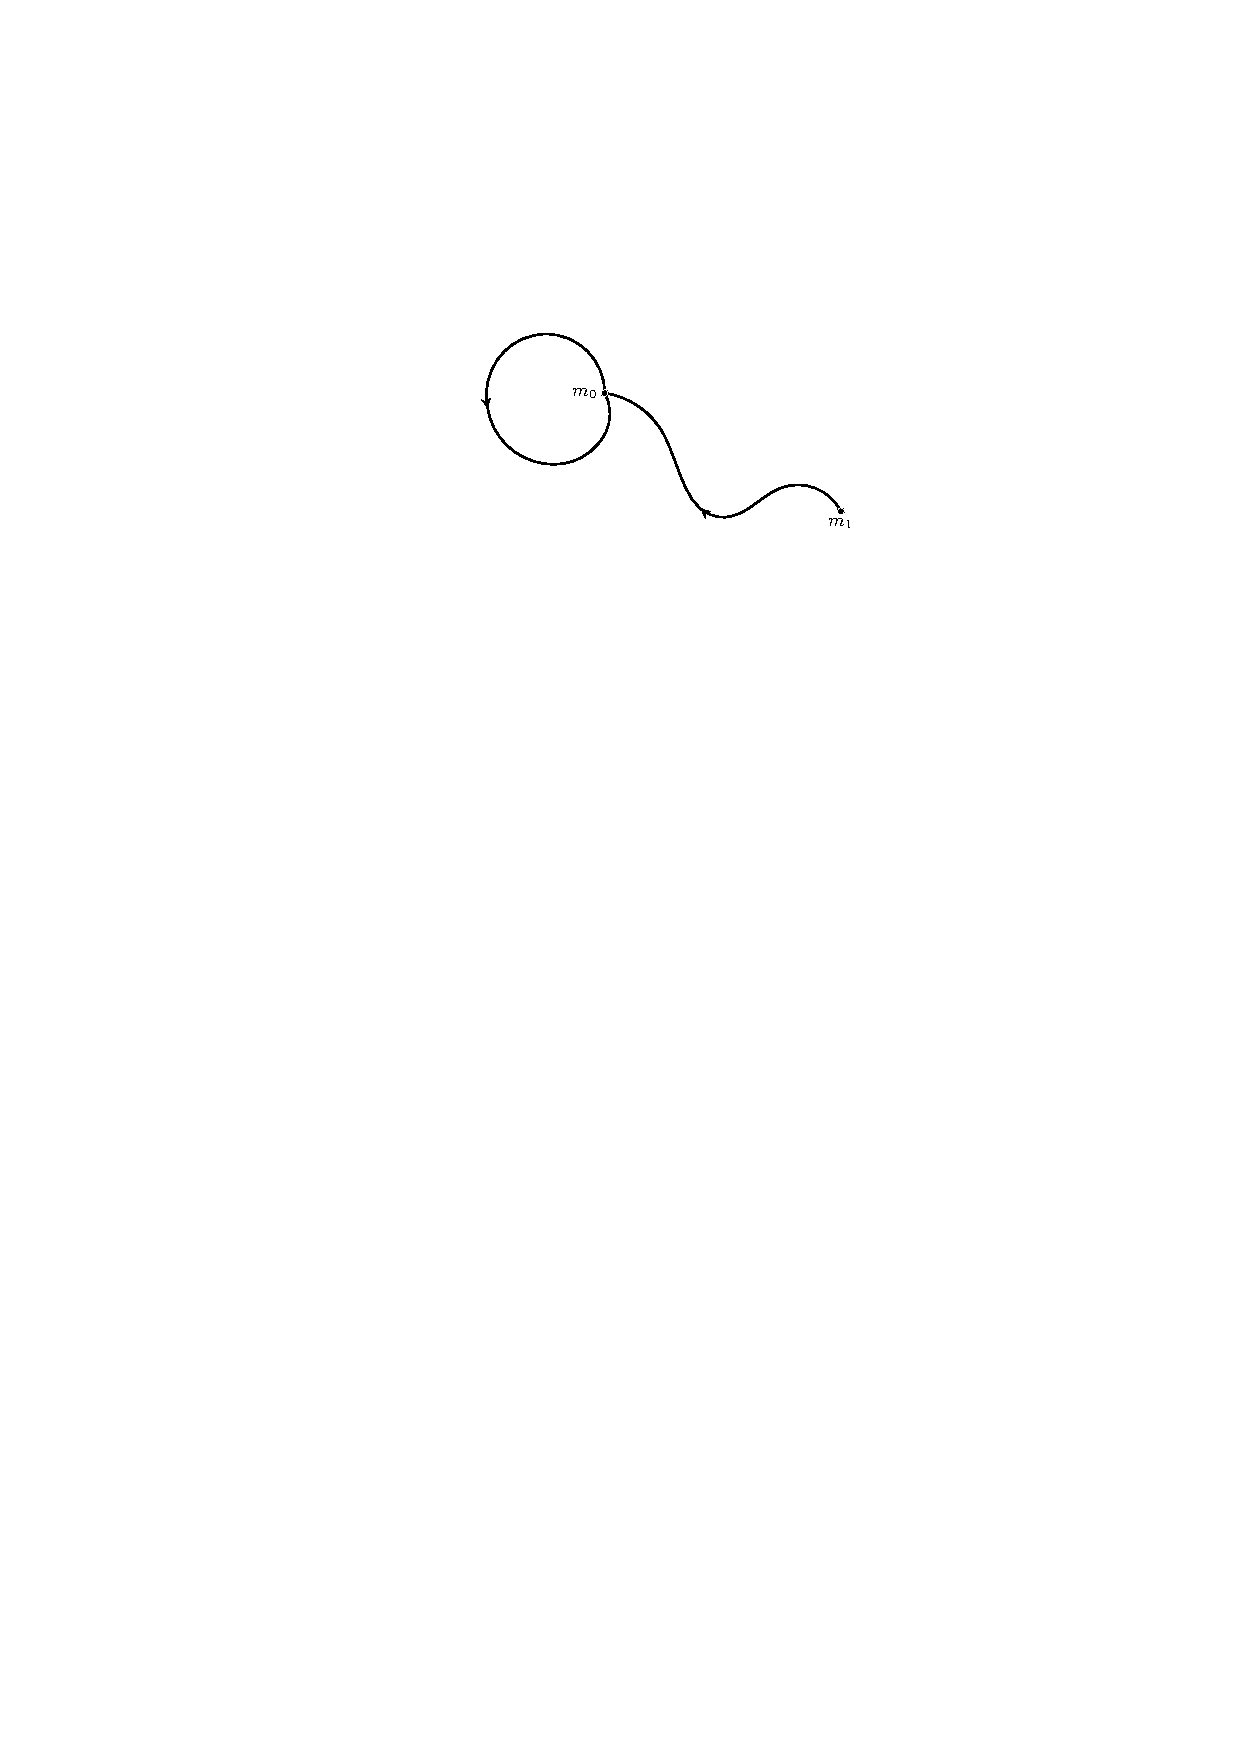
\includegraphics[scale=0.8]{figures/holonomy.pdf}
    \end{center}
    All restricted $\omega$-holonomy at $p_1$ arises in this way. Since $p(t)$ is $\omega$- and $\omega'$-horizontal, the holonomy along the lasso agrees between the two connections.  The new holonomy algebra contains the contributions of these lassos, which are of the same dimension for both connections, so it contains the restricted holonomy of $\omega$.
\end{proof}


Similarly, the next lemma shows that any principal $G$-connection can be deformed on an arbitrarily small compact set so as to make the restricted holonomy group be all of the identity component $G_0$. If $G$ is connected, then this proves the existence of irreducible connections on any principal $G$-bundle.

\begin{lem}\label{lem 16.24 McKay}
    Let $P(G,M)$ be a principal bundle over a connected base $M$ of dimension $\dim M\geq 2$. Then (1) $P$ admits a principal connection whose restricted holonomy group is the identity component $G_0$ and (2) for any principal connection $\omega$ and any open set $\varnothing\neq U\subset M$, there exists a principal connection $\omega'$ whose restricted holonomy group is $G_0$ and which agrees with $\omega$ outside of a compact subset of $U$.
\end{lem}
\begin{proof}
    Suppose that the result is proven for trivial bundles. Then we can choose a $U$ over which the bundle is trivial and the result follows. Thus, it suffices to consider a trivial bundle $P=M\times G$ with the standard flat connection $\omega=\pr_G^\ast\theta_G$.

    If $\frakg=0$, the result is trivial. Otherwose, take $m_1\in M$ and a curvature value $\Omega_1=\Omega_{p_1}$ which takes on a nonzero value $\Omega_1(X,Y)$ for some $X,Y\in\T_{p_1}P$ over $m_1$. Take a relatively compact set $U_1$ around $m_1$ whose closure is not $M$. Pick a connection over $U_1$ whose curvature at $p_1$ is $\Omega_1$. Use a \gls{pou} to glue this connection to $\omega$, so that it agrees with $\omega$ outside of $\restr{P}{U_1}$. Call the resulting connection $\omega'$. The holonomy algebra now has dimension at least $1$.

    After $k$ steps, assume that the holonomy algebra is of dimension at least $k$. Suppose that there is some point at which the holonomy algebra is still not $\frakg$. Then this is true at every point, because the holonomy algebra changes only by adjoint action from point to point. Take some $m_{k+1}\in M$ near which $\omega$ is flat, a point $p_{k+1}\in P_{m_{k+1}}$, and a curvature element $\Omega_{k+1}$ taking on some value $\Omega_{k+1}(X,Y)$ at $p_{k+1}$ outside of the holonomy algebra. Take a relatively compact open set $U_{k+1}$ around $m_{k+1}$ with closure not intersecting any of the closures of the previously chosen open sets $U_i$. Over $U_{k+1}$, pick a connection whose curvature at $p_{k+1}$ is $\Omega_{k+1}$. Use a \gls{pou} to glue this connection to $\omega$, so that it agrees with $\omega$ outside of $\restr{P}{U_{k+1}}$. By induction, we will at some point enlarge the restricted holonomy to the point of being an open subgroup, and hence all of $G_0$.
\end{proof}

It is quite rare that we can explicitly find the holonomy bundle, as it requires solving equations of Lie type. Hence we might not know its tangent spaces, and cannot directly apply the Ambrose-Singer Theorem. Instead, by purely local calculation, we can find the smallest Lie algebra $\frakn< \frakg$ containing all values of the curvature at all points, at least constraining the holonomy algebra. Since the curvature transforms in the adjoint representation, this Lie algebra contains all $G$-adjoint conjugates of the holonomy algebra.

\begin{thm}[Cartan's holonomy envelope (1926)]\label{thm 16.26 McKay}
    Let $P(G,M)$ be a principal bundle over a connected base $M$ with a principal connection $\omega$. Let $\frakn<\frakg$ be the span of the values of the curvature $\Omega$ at all points of $P$. Then 
    \begin{enumerate}
        \item $\frakn\sub \frakg$ is an ideal containing the holonomy algebra. 
        \item Further, suppose that $N\sub G$ is a normal subgroup with Lie algebra $\frakn$. Then the restricted holonomy groups at all points of $P$ lie in $N$, and if the full holonomy group at some point of $P$ lies in $N$, then so does the holonomy group at any point.
        \item The distribution $\omega^{-1}(\frakn)$ is integrable and each leaf of the corresponding foliation contains a holonomy bundle.
    \end{enumerate}
\end{thm}
\begin{proof}
    Let $V_{p}=\<\Omega(X,Y)\mid X,Y\in\T_{p}P\><\frakg$. Then $\frakn$ is the span of the union of the $V_{p}$ over all $p\in P$. The curvature transforms under the adjoint representation, so $V_p$ does as well, and so $\frakn$ is an $\Ad(G)$-invariant subspace, hence also $\ad(\frakg)$-invariant, i.e., an ideal. 

    We assume that $P$ is a right bundle as usual. Under the principal action, holonomy transforms by conjugation, $\Hol_{p\cdot g}(\omega)=\Adg_g^{-1}\Hol_p(\omega)$. By the normality of $N$, the holonomy lies in $N$ at some point iff it lies in $N$ at all points of the same fiber. But then we can follow horizontal curves to get from fiber to fiber, because $M$ is connected. The holonomy doesn't change along horizontal curves, so it lies in $N$ everywhere.

    Consider the $1$-form $\omega+\frakn\in\Omega^1(P;\frakg\slash\frakn)$. From the equation $\Omega=\dd\omega+\frac12[\omega,\omega]$, we see that, modulo $\omega+\frakn$,
    \[\dd\omega+\frakn\equiv \Omega+\frakn\equiv 0\pmod{\omega+\frakn},\]
    since $\Omega$ is valued in $\frakn$ and $[\frakn,\frakn]<\frakn$. By the Frobenius Theorem, $P$ is foliated by submanifolds whose tangent spaces consist of the tangent vectors $X$ on which $\omega(X)\in\frakn$. In particular, the horizontal directions $\ker\omega$ lie tangent to the leaves. Hence, each leaf contains a holonomy bundle.
\end{proof}

\begin{rem}
    Suppose that we wish to determine whether the holonomy group of a principal bundle $P(G,M)$ with principal connection, on a connected and simply connected manifold $M$, is up to conjugacy equal to some subgroup $L<G$. First, for this to hold, at every point of $P$ the curvature values must lie in some conjugate of the Lie algebra $\frakl<\frakg$. Second, if $P'\subset P$ is the subset of points at which the curvature is valued in $\frakl$, then $P'$ must contain a holonomy bundle. To check for this, we can compute $P'$ by a local calculation, without knowing how to compute the holonomy group, just by calculating the curvature. Replace $P'$ by the set of points of $P'$ at which all integral curves of all vector fields $X\in\fX(P)$ with $\omega(X)\in\frakl$ stay, at least for a short time, inside $P'$ (this might be trickier but is still local). Repeat this process of replacing $P'$ by that subset of $P'$. After we repeat infinitely many times, if $P'$ is still not empty, then, as in the proof of the last theorem, the equations $\omega+\frakl=0$ satisfy the requirements of the Frobenius Theorem so that the horizontal directions are tangent to the leaves, so contain a holonomy bundle and the holonomy group lies in $L$, at least locally.
\end{rem}








\section{Gauge transformations}


Let us discuss the connection to the gauge group. The Lie algebra of the group of automorphisms (not only vertical ones) $\Aut(P)$ is the space $\aut(P)=\fX(P)^G$ of $G$-invariant vector fields on $P$, and the Lie algebra of the gauge group (of vertical automorphisms) is the subspace $\gau(P)$ of vertical $G$-invariant vector fields. One has the exact sequence of Lie algebras
\[0\to \gau(P)\to \aut(P)\to \fX(M)\to 0.\]
The surjectivity of the map $\aut(P)\to \fX(M)$ can be proved using a trivializing open covering of $M$ and a $\gls{pou}$ subordinate to that cover. 


For $\varphi\in \Hom_G(P,G)$, the corresponding vertical automorphism is given by
\[\vartheta_\varphi:P\to P,\quad p\mapsto p\cdot \varphi(g).\label{eq 1.8.2 RS2}\]
The equivariance property $\vartheta_\varphi(p\cdot g)=\vartheta_\varphi(p)\cdot g$ is clearly equivalent to $\varphi(p\cdot g)=g^{-1}\varphi(p)g$, which is exactly the defining property of $\Hom_G(P,G)$. It is also easy to check that this correspondence is a group isomorphism (where elements of $\Hom_G(P,G)$ are multiplied pointwise, so $\vartheta_\varphi\circ\vartheta_\psi=\vartheta_{\varphi\cdot\psi}$). Finally, recall from Proposition~\ref{prop 1.2.6 RS2} that the space $\Hom_G(P,G)$ can be identified with the space of sections of the associated group bundle $\Adg(P)=P\times^G G$, where $G$ acts on itself by conjugations. We thus have the isomorphisms
\[\Aut(P)\cong \Hom_G(P,G)\cong \Gamma^\infty(\Adg(P)).\]

It is also obvious that every vertical automorphism $\vartheta_\varphi\in\Gau(P)$ induces a vertical automorphism $\wh\vartheta_\varphi$ of any associated bundle $P^{[\sigma]}=P\times^G F$ given by
\[\wh\vartheta_\varphi([(p,f)])=\left[(p,\sigma_{\varphi(p)}(f))\right].\]
In particular, if $G\overset{\sigma}{\acts}F$ is a linear representation, then $\wh{\vartheta}_\varphi$ is a vertical automorphism of vector bundles.


\begin{prop}[{{\cite[Prop.~1.8.7]{RS2}}}]
    Let $(P\overset{\pi}{\to}M,G,\Phi)$ be a principal bundle and let $\calH P$ be a principal connection. Then, for $\vartheta\in \Gau(P)$ corresponding to $\varphi\in \Hom_G(P,G)$, one has the following transformation laws:
    \begin{enumerate}
        \item If $\omega$ is the connection form of $\calH P$, then $\vartheta^\ast \omega$ is the connection form of $\vartheta_\ast^{-1}(\calH P)$ and 
        \[(\vartheta^\ast\omega)_p=\Ad_{\varphi(p)}^{-1}\circ\omega_p+(\varphi^\ast\theta_G)_p,\label{eq 1.8.7 RS2}\]
        where $\theta_G$ is the Maurer-Cartan form on $G$.

        \item If $\Omega^\omega$ is the curvature $2$-form of $\omega$, then $\vartheta^\ast\Omega^\omega$ is the curvature form of $\vartheta^\ast\omega$ and
        \[(\vartheta^\ast\Omega)_p=\Ad_{\varphi(p)}^{-1}\circ\Omega_p.\label{eq 1.8.8 RS2}\]
    \end{enumerate}
\end{prop}
\begin{proof}
    1. To prove the first equality, we must calculate $\vartheta_\ast(X)$ for $X\in \T_pP$. Let $\gamma$ be a path in $P$ representing $X$.  Using \eqref{eq 1.8.2 RS2}, we have
    \begin{multline}
        \vartheta_{\ast p}(X)=\restr{\frac{\dd}{\dd t}}{0}\vartheta(\gamma(t))=\restr{\frac{\dd}{\dd t}}{0} (\gamma(t)\cdot \varphi(\gamma(t)))=
        \\=\restr{\frac{\dd}{\dd t}}{0}(\gamma(t)\cdot \varphi(p))+\restr{\frac{\dd}{\dd t}}{0}(p,\varphi(\gamma(t))=\Phi_{\varphi(p)\ast}(X)+\Phi_{p\ast}\circ \varphi_{\ast p}(X).
    \end{multline}
    The second term describes a vertical vector in $\vartheta(p)$. Thus, we may write it in the form $\Phi_{\vartheta(p)\ast}(A)$ with $A\in\frakg$. Explicitly, since $\varphi_{\ast p}(X)\in \T_{\varphi(p)}G$, we can write
    \[\Phi_{p\ast}\circ \varphi_{p\ast }(X)=\Phi_{p\ast}\circ \rmL_{\varphi(p)\ast}\circ \rmL_{\varphi(p)\ast}^{-1}\circ \varphi_{\ast p}(X).\]
    Using
    \[\rmL_{\varphi(p)\ast}^{-1}\circ \varphi_{p\ast}(Y)=\theta_G(\varphi_{p\ast}(X))=(\varphi^\ast\theta_G)_p(X)\]
    and $\Phi_p\circ \rmL_{\varphi(p)=\Phi_{\vartheta(p)}}$, we obtain
    \[\vartheta_{p\ast}(X)=\Phi_{\varphi(p)\ast}(X)+\Phi_{\vartheta(p)\ast}(\varphi^\ast\theta_G(X)).\label{eq 1.8.10 RS2}\]
    Using this equation, together with the equivariance of $\omega$, we obtain \eqref{eq 1.8.7 RS2}.

    2. Using the structure equation, we obtain
    \[\vartheta^\ast\Omega=\vartheta^\ast\left(\dd \omega+\frac12[\omega,\omega]\right)=\dd(\vartheta^\ast\omega)+\frac12[\vartheta^\ast\omega,\vartheta^\ast\omega],\]
    that is, $\vartheta^\ast\Omega$ is the curvature form of $\vartheta^\omega$, indeed. To prove \eqref{eq 1.8.8 RS2}, we must calculate $\vartheta^\ast \Omega(X,Y)$ for any $X,Y\in \T_pP$. For that purpose, we use the decomposition \eqref{eq 1.8.10 RS2} for both vectors. Since $\Omega$ is horizontal, only the first terms of this decomposition contribute. Then, using the equivariance of $\Omega$, one immediately obtains \eqref{eq 1.8.8 RS2}.
\end{proof}

\begin{rem}\label{rem 1.8.8 RS2}
    \begin{enumerate}
        \item Sometimes we will use the following short-hand notation for the above transformation laws:
        \[\vartheta^\ast\omega=\Ad_{\varphi}^{-1}\circ\omega+\varphi^\ast\theta_G,\quad \vartheta^\ast \Omega=\Ad_\varphi^{-1}\circ\Omega.\]
        In matrix notation, we have $\varphi^\ast\theta_G=\varphi^{-1}\dd\varphi$, and 
        \[\vartheta^\ast\omega=\varphi^{-1}\omega\varphi+\varphi^{-1}\dd\varphi,\quad \vartheta^\ast\Omega^\omega=\varphi^{-1}\Omega^\omega \varphi.\]
        \item Using the local representative $\rho^\alpha=\varphi\circ s_\alpha$, we read off the following transformation laws for the local representatives of $\omega$ and $\Omega^\omega$:
        \[\scrA'=\Ad_\rho^{-1}\circ\scrA+\rho^\ast\theta_G,\quad \scrF'=\Ad_\rho^{-1}\scrF.\]
        Note that this formula is essentially identical to the transformation law for local representatives from Corollary~\ref{cor 1.3.12 RS2}. We might call the transformation coresponding to a change of local coordinates a \emph{passive gauge transformation}, and a transformation stemming from an actual automorphism of the bundle an \emph{active gauge transformation}.
    \end{enumerate}
\end{rem}


Since we would like to study bundles up to isomorphism, the action of the gauge group $\Gau(P)=\Aut_M(P)$ on the space of connections $\calA(P)$ will be crucial. We will now characterize the infinitesimal version of this action. The gauge algebra $\gau(P)$ can be identified with sections of the adjoint bundle $\Ad(P)$: \index{Adjoint vector bundle}
\[\gau(P)\cong \Omega^0(M;\Ad(P))=\Omega^0_{\hor}(P;\frakg)^\Ad.\]
Indeed, each $G$-invariant vector field $X\in\Gamma^\infty(\calV P)$, by composition with the global trivialization $\psi^{-1}:\calV P\to P\times\frakg$ (cf.\ Lemma~\ref{lem 1.3.1 RS2}), produces an element of $\Omega^0_{\hor}(P;\frakg)^\Ad$.

An automorphism $\vartheta\in\Aut(P)$ acts on $\calA(P)$ by pullbacks along the inverse, $\omega\mapsto \vartheta_\ast\omega$. For the action of the subgroup $\Gau(P)$, there is an alternative formula for this action which we now derive. 

Recall that each vertical automorphism $\vartheta\in \Gau(P)$ corresponds to a unique equivariant function $\varphi:P\to G$ defined by 
\[\varphi\in \Hom_G(P,G),\quad \vartheta(p)=p\cdot \varphi(p)^{-1}.\]
Here, $G$ acts on itself by conjugations, and the equivariance property reads $\varphi(p\cdot g)=g^{-1}\varphi(p)g$ (which immediately follows from $\vartheta(p\cdot g)=\vartheta(p)\cdot g$). Similarly, each invariant vertical vector field $Y\in \gau(P)$ can be identified, via the global trivialization $\psi^{-1}$, with a function 
\[\wt\zeta\coloneqq \psi^{-1}\circ Y\in \Omega^0_{\hor}(P;\frakg)^\Ad.\]
Indeed, it is easy to check that $\Phi_g^\ast \zeta=\Ad_g^{-1}\zeta$. This, in turn, is identified via Proposition~\ref{prop 1.2.12 RS2} with a section of the associated adjoint bundle: \index{Adjoint vector bundle}
\[\zeta\in \Omega^0(M;\Ad(P))=\Gamma^\infty(\Ad(P)).\]
Explicitly, the identification is $\zeta(m)=\iota_p(\wt\zeta(p))=[(p,\wt\zeta(p))]\in P\times^G \frakg$, where $p\in P_m$.
We can write these identifications as isomorphisms
\[\gau(P)\cong \Omega^0_{\hor}(P;\frakg)^\Ad\cong \Gamma^\infty(\Ad(P)).\]
The next proposition computes the action of the gauge group on the Lie algebra of all infinitesimal automorphisms.

\begin{prop}
    Let $\vartheta\in\Gau(P)$ and $\varphi\in \Hom_G(P,G)$ the corresponding equivariant function. For all $X\in\aut(P)=\fX(P)^G$,
    \[\vartheta_\ast X-X\in\gau(P).\]
    The corresponding section $\zeta \in\Gamma^\infty(\Ad(P))$ is represented by the equivariant function
    \[\wt\zeta(p)=\Ad_{\varphi(p)}\circ(\varphi^\ast \theta_G)(X(p)),\quad p\in P.\]
\end{prop}
\begin{proof}
    The vector field $\vartheta_\ast X$ is invariant since $\vartheta$ commutes with the principal $G$-action, and under $\pi_\ast$ projects onto the same vector field as $X$ since $\pi\circ\vartheta=\pi$. This shows that $Y=\vartheta_\ast X-X$ is vertical and $G$-invariant, thus an element of $\gau(P)$. Now we evaluate both sides of \eqref{eq 1.8.7 RS2} on the vector field $X$:
    \[\omega(\vartheta_\ast X)=\Ad_{\varphi}^{-1}\circ \omega(X)+(\varphi^\ast \theta_G)(X),\]
    which is equivalent to
    \[\Ad_\varphi\omega(\vartheta_\ast X)-\omega(X)=\Ad_\varphi\circ (\varphi^\ast \theta_G)(X),\]
    By the equivariance of principal connections, $\Ad_\varphi\omega(\vartheta_\ast X)=\omega(\Phi_{\varphi\ast}^{-1}\vartheta_\ast X)$, and because $\vartheta$ is equivariant and $X$ is invariant, this is just $\omega(\vartheta_\ast X)$. Therefore
    \[\omega(Y)=\Ad_\varphi\circ (\varphi^\ast \theta_G)(X).\]
    The connection form was defined as $\omega=\psi^{-1}\circ\calV$. Since $Y$ is vertical, $\omega(Y)=\psi^{-1}(Y)$. We get the corresponding $\Ad$-equivariant function
    \[\wt{\zeta}=\psi^{-1}\circ Y=\Ad_\varphi\circ (\varphi^\ast\theta_G)(X).\]
\end{proof}

\begin{rem}
    Note that $\Ad_\varphi\circ \varphi^\ast\theta_G$ can also be written as $\varphi^\ast\theta_G^R$, where $\theta_G^R$ is the right-invariant Maurer-Cartan form on $G$. Therefore, in matrix notation we may write $\wt\zeta=(\Lie_X\varphi)\cdot \varphi^{-1}$.
\end{rem}

\begin{prop}\label{prop action of Gau(P) on calA(P)}
    The natural action of $\Gau(P)$ on $\calA(P)$ is given by
    \[\vartheta\cdot\omega\coloneqq (\vartheta^{-1})^\ast\omega=\Ad_\varphi \circ (\omega-\varphi^\ast \theta_G),\quad \omega\in\calA(P),\]
    where $\varphi\in \Hom_G(P,G)$ is the element representing $\vartheta\in \Gau(P)$.
\end{prop}
\begin{proof}
    We will prove the equivalent property $\vartheta^\ast\omega=\Ad_\varphi^{-1}\omega+\varphi^\ast\theta_G$. It suffices to check this on invariant vector fields $X\in \fX(G)^G$. By the last proposition, and since $\varphi^\ast f=\Ad_\varphi^{-1}f$ for all $f\in \Omega^0_{\hor}(P;\frakg)^\Ad$, 
    \[(\vartheta^\ast\omega)(X)=\vartheta^\ast(\omega(\vartheta_\ast X))=\Ad_\varphi^{-1}(\omega(\vartheta_\ast X))=(\Ad_\varphi^{-1}\omega+\varphi^\ast\theta_G)(X).\]
\end{proof}

We can now characterize the stabilizer subgroups $\Gau(P)_\omega$ of gauge transformations that preserve a given connection $\omega$. First consider how gauge transformations affect parallel transport. The following is a simple exercise.

\begin{lem}\label{lem 31794}
    Let $\vartheta\in\Gau(P)$ and $\vartheta_m\coloneqq\restr{\vartheta}{P_m}$. Then for any path $\gamma:[0,1]\to M$, 
    \[\tra_{\gamma}^{\vartheta\cdot\omega}=\vartheta_{\gamma(1)}\circ\tra_\gamma^\omega \circ\vartheta_{\gamma(0)}^{-1}.\]
\end{lem}

Now suppose $M$ is connected and recall the holonomy representation for $m\in M$:
\[\Hol(\omega):C(m)\to \Diff(P_m)^G\cong G,\quad \gamma\mapsto \tra_\gamma^\omega.\]
Its image $\Hol_p(\omega)< G$ is the holonomy group based at $p\in P_m$, and its identity component $\Hol^0_p(\omega)\emb G$ is a closed subgroup of $G$. Recall also that $\Diff(P_m)^G\cong G$ is a natural isomorphism, so we will use these two groups interchangeably.

\begin{prop}\label{prop gauge group of principal connection}
    The restriction map $\Gau(P)_\omega\to \Diff(P_m)^G$, $\vartheta\mapsto \vartheta_m\coloneqq\restr{\vartheta}{P_m}$ is injective and defines an isomorphism of the stabilizer $\Gau(P)_\omega$ with the centralizer in $G$ of the holonomy group:
    \[\Gau(P)_\omega\cong \rmC_G(\Hol_p(\omega)).\]
\end{prop}
\begin{proof}
    A gauge transformation preserves $\omega$ iff it preserves $\calH P$. Equivalently, by Lemma~\ref{lem 31794} (applied to $\vartheta^{-1}$), $\vartheta\in\Gau(P)_\omega$ iff for all paths $\gamma:[0,1]\to M$, $\vartheta$ commutes with parallel transport:
    \[\vartheta(\gamma(1))=\tra_\gamma^\omega\circ \vartheta(\gamma(0))\circ(\tra_\gamma^\omega)^{-1}.\label{18041}\]
    Taking paths with $\gamma(0)=m$, it follows that if $\vartheta_m=\id_{P_m}$, then $\vartheta=\id_P$. That is, the map $\vartheta\mapsto\vartheta_m$ is injective. Taking $\gamma\in C(m)$, \eqref{18041} shows that $\vartheta_m$ centralizes $\Hol_p(\omega)$. Conversely, if $\vartheta_m\in \rmC_G(\Hol_p(\omega))$, then we can define $\vartheta$ fiberwise by putting
    \[\vartheta_{m'}\coloneqq \tra_\gamma^\omega\circ \vartheta_m\circ (\tra_\gamma^\omega)^{-1},\]
    where $\gamma$ is any path $m\leadsto m'$. The condition $\vartheta\in \Gau(P)_\omega$ guarantees that the right hand side does not depend on the choice of $\gamma$ and hence globally defines a smooth automorphism.
\end{proof}

\begin{rem}\label{rem automorphisms of principal connection}
    While this shows that the set of gauge transformations (vertical automorphisms) preserving a principal connection is a Lie group, the same does not hold, in general, for the set of \emph{all} automorphisms that preserve a connection. For example, the canonical flat connection on the product bundle $P=M\times G$ admits an automorphism $(m,g)\mapsto (f(m),g)$, for each diffeomorphism $f$ of $M$ (indeed, it obviously preserves the horizontal distribution). This stands in marked difference from the situation with Cartan connections, whose automorphism groups are always finite-dimensional Lie groups.
\end{rem}

This shows that all stabilizer subgroups are finite-dimensional Lie groups. In particular, for an irreducible connection, the stabilizer of a connection $\omega$ is isomorphic to the center $\rmZ(G)$. This is another way of detecting reducibility, in addition to the Ambrose-Singer Theorem~\ref{thm 1.7.15 RS2 Ambrose-Singer}. Moreover:

\begin{cor}
    The based gauge group $\Gau_m(P)\coloneqq \{\vartheta\in \Gau(P)\mid \vartheta_m=\id_{P_m}\}$ acts freely on $\calA(P)$.
\end{cor}
\begin{cor}
    If $G$ is abelian, every principal connection has stabilizer equal to $G$, viewed as constant gauge transformations in $\Gau(P)\cong \Gamma^\infty(\Adg(P))\cong C^\infty(M,G)$.
\end{cor}

\begin{defn}[Moduli space of connections]\index{Moduli space}
    The (topological) quotient $\calM(P)\coloneqq \calA(P)\slash \Gau(P)$ is called the moduli space of connections. 
\end{defn}

The moduli space consists of classes of gauge-equivalent gauge potentials, the `true' configuration space in gauge theory. One can show that the map 
\[\calA(P)\times\Gau(P)\to \calA(P)\times\calA(P),\quad (\omega,\vartheta)\mapsto (\omega,\vartheta\cdot\omega),\]
is closed and that the stabilizers $\Gau(P)_\omega$ are compact, so that the action of $\Gau(P)\acts\calA(P)$ is proper \cite[Thm.~6.1.7]{RS2}. Hence, the orbits are closed and the moduli space is Hausdorff. This moduli space is still ``infinite-dimensional''. To get nicer moduli spaces one usually restricts to a sub-class of connections such as flat connections or, more generally, Yang-Mills connections.







\section{Covariant exterior derivative}\label{sec: cov ext derivative}



In the previous \sect\ we computed the natural action of the gauge group $\Gau(P)$ on the space of connections $\calA(P)$. As is clear from Proposition~\ref{prop action of Gau(P) on calA(P)}, this is in fact a smooth action of an infinite-dimensional Lie group on an infinite-dimensional smooth manifold. The natural question is then: what is the infinitesimal action, or what are the Killing vector fields corresponding to this action? Since $\calA(P)$ is an affine space modeled on $\Omega^1_{\hor}(P;\frakg)^\Ad$, its tangent spaces are naturally identified with the same space:
\[\T_\omega\calA(P)\cong \Omega^1_{\hor}(P;\frakg)^\Ad.\]
Thus, an infinitesimal gauge transformation $\zeta\in\Omega^0_{\hor}(P;\frakg)^\Ad\cong\gau(P)$ generates a Killing vector field $\zeta_\ast\in \fX(\calA(P))\cong C^\infty(\calA(P),\Omega^1_{\hor}(P;\frakg)^\Ad)$. In other words, the map $(\zeta,\omega)\mapsto\zeta_\ast(\omega)$ is an object that takes a horizontal $0$-form $\zeta$ (of type $\Ad$) and a connection form $\omega$, and produces a horizontal $1$-form (again of type $\Ad$). This is exactly the missing analog of an exterior derivative on these spaces of sections! We now turn to studying this object.

\begin{prop}
    The Killing vector field generated by an infinitesimal gauge transformation $\zeta\in\Gamma^\infty(\Ad(P))\cong\gau(P)$ on $\calA(P)$ is given by
    \[-\zeta_\ast(\omega)=\dd \wt{\zeta}+[\omega,\wt{\zeta}],\quad \omega\in\calA(P),\]
    where $\wt{\zeta}\in \Omega^0_{\hor}(P;\frakg)^\Ad$ is the corresponding equivariant function.
\end{prop}
\begin{proof}
    Let $\gamma:(-\epsilon,\epsilon)\to \Gau(P)$ be a path in $\Gau(P)$ such that $\dot\gamma(0)=\zeta$ (where we think of $\zeta$ as an element of $\gau(P)$ directly). Let $\wt\gamma$ be the corresponding path in $\Omega^0_{\hor}(P;\frakg)^\Ad$. We have $\dot{\tilde{\gamma}}(0)=\wt{\zeta}$. Then, by Proposition~\ref{prop action of Gau(P) on calA(P)},
    \[-\zeta_\ast(\omega)=\restr{\frac{\dd}{\dd t}}{0}(\gamma(-t)\cdot \omega)=\restr{\frac{\dd}{\dd t}}{0}\left(\Ad_{\wt{\gamma}(-t)}(\omega-(\wt{\gamma}(-t))^\ast\theta_G)\right)=[\omega,\wt{\zeta}]+\dd\wt{\zeta},\]
    where the last equality follows from the definition of the Lie bracket on a Lie group and the definition of the Maurer-Cartan form.
\end{proof}


Since the action of the gauge group is a left action, the minus sign above is convenient to make the map to Killing vector fields a homomorphism of Lie algebras. Now observe that due to $\wt{\zeta}$ being of type $\Ad$, we can rewrite the Lie bracket above as a Lie derivative along a Killing vector field $\omega(X_p)_\ast(p)=\psi(\omega(X_p))=\calV(X_p)$ and simplify:
\[(\dd\wt{\zeta}+[\omega,\wt{\zeta}])(X)=
\dd\wt\zeta(X)-\Lie_{\omega(X)_\ast}\wt\zeta=
\dd\wt\zeta(X)-\dd\wt\zeta(\calV(X))=\dd\wt{\zeta}(\hor X).\label{eq 4791793}\]

This, as well as the definition of curvature, suggests the following general definition. Note that at this point we have to specialize to associated \emph{vector} bundles, although slight generalizations are possible.

\begin{defn}[Covariant exterior derivative]
    Let $P$ be a principal bundle with a principal connection $\calH P$ and connection form $\omega$, let $V$ be a finite-dimensional vector space, and let $\alpha\in\Omega^k(P;V)$. The covariant exterior derivative of $\alpha$ w.r.t.\ $\omega$ is defined as
    \[(\rmD^\omega \alpha)(X_0,\ldots,X_k)\coloneqq \dd\alpha(\hor X_0,\ldots,\hor X_k),\quad X_0,\ldots,X_k\in\fX(P).\]
    By definition, $\rmD^\omega$ fulfills the same Leibniz rule (w.r.t.\ $\wedge$) as the ordinary exterior derivative and $\rmD^\omega \alpha$ is horizontal. Moreover, as we will show below, $\rmD^\omega$ preserves the symmetry type of any horizontal form.
\end{defn}

In particular, the curvature form $\Omega^\omega$ satisfies 
\[\Omega^\omega=\rmD^\omega\omega.\]
Now we derive a general formula for the covariant exterior derivative.

\begin{prop}[{{\cite[Prop.~1.4.3]{RS2}}}]\label{prop 1.4.3 RS2}
    Let $P(M,G)$ be a principal bundle, let $G\overset{\sigma}{\acts}V$ be a finite-dimensional linear representation, and let $\omega$ be a principal connection form on $P$.
    \begin{enumerate}
        \item $\rmD^\omega(\Omega^k_{\hor}(P;V)^\sigma)\subset \Omega^{k+1}_{\hor}(P;V)^\sigma$.
        \item Let $\wt\alpha\in\Omega^k_{\hor}(P;V)^\sigma$. Then
        \[\rmD^\omega\wt\alpha=\dd\wt\alpha+\sigma_\ast(\omega)\wedge \wt\alpha,\label{eq 1.4.1 RS2}\]
        where
        \[(\sigma_\ast(\omega)\wedge\wt\alpha)_p(X_0,\ldots,X_k)\coloneqq \sum_{i=0}^k (-1)^i\sigma_\ast(\omega_p(X_i))\left(\wt\alpha_p(X_0,\ldots,\wh{X}_i,\ldots,X_k)\right),\]
        with $p\in P$, $X_0\ldots,X_k\in \T_pP$, and where the hat represents an omitted argument.
    \end{enumerate}
\end{prop}
\begin{proof}
    1. Let $\wt\alpha\in\Omega^k_{\hor}(P,V)^\sigma$. By definition of the covariant exterior derivative, $\rmD^\omega\wt\alpha$ is a $V$-valued horizontal $(k+1)$-form. We now check equivariance:
    \begin{align}
        (\Phi_g^\ast \rmD^\omega\wt\alpha)(X_0,\ldots,X_k)&=\rmD^\omega\wt\alpha(\Phi_{g\ast}X_0,\ldots, \Phi_{g\ast}X_k)=\notag\\
        &=\dd\wt\alpha(\hor\Phi_{g\ast}X_0,\ldots,\hor \Phi_{g\ast}X_k)=\notag\\
        &=\dd\wt\alpha(\Phi_{g\ast}\hor X_0,\ldots,\Phi_{g\ast}\hor X_k)=\notag\\
        &=\dd(\Phi_g^\ast\wt\alpha)(\hor X_0,\ldots,X_k)=\notag\\
        &=\dd(\sigma_{g^{-1}}\circ\wt\alpha)(\hor X_0,\ldots,\hor X_k)=\notag\\
        &=\sigma_{g^{-1}}\circ \rmD^\omega\wt\alpha (X_0,\ldots,X_k).
    \end{align}
    This shows that $\rmD^\omega\wt\alpha$ is of type $\sigma$.

    2. Since each of the vectors $X_0,\ldots,X_k\in \T_pP$ may be decomposed into a vertical and a horizontal part, it is enough to consider the usual cases:
    \begin{enumerate}[label=(\alph*)]
        \item Let all $X_i$ be horizontal. Let $\omega(X_i)=0$ and formula \eqref{eq 1.4.1 RS2} follows from the definition of $\rmD^\omega$.
        \item Let one of the vectors $X_i$, say $X_0$, be vertical and the rest horizontal. Then, there exists an element $A\in\frakg$ such that $X_0=(A_\ast)_p=\Phi^0_\ast(A)$ and a family of vector fields $Y_1,\ldots,Y_k\in\fX(M)$ such that their horizontal lifts $Y_i^h$ at $p$ coincide with the vectors $X_1,\ldots,X_k$. Then
        \[(\rmD^\omega\wt\alpha)(X_0,\ldots,X_k)=0,\; (\sigma_\ast(\omega)\wedge\wt\alpha)(X_0,\ldots,X_k)=\sigma_\ast(A)(\wt\alpha(X_1,\ldots,X_k)).\]
        Using Proposition~\ref{prop 4.1.6 RS1}, Lemma~\ref{lem 1.4.2 RS2}, the horizontality of $\wt\alpha$ and the $G$-invariance of horizontal lifts, we calculate
        \begin{align}
            (\dd\wt\alpha)_p(X_0,\ldots,X_k)&=(A_\ast)_p(\wt\alpha(Y_1^h,\ldots,Y_k^h))=\notag\\
            &=\restr{\frac{\dd}{\dd t}}{0}\wt\alpha_{p\cdot \rme^{tA}}(Y_1^h,\ldots,Y_k^h)=\notag\\
            &=\restr{\frac{\dd}{\dd t}}{0}\wt\alpha_{p\cdot \rme^{tA}}((\Phi_{\rme^{tA}})_\ast X_1^h,\ldots,(\Phi_{\rme^{tA}})_\ast X_k^h)=\notag\\
            &=\restr{\frac{\dd}{\dd t}}{0}\left(\Phi_{\rme^{tA}}^\ast\wt\alpha\right)_p(X_1,\ldots,X_k)=\notag\\
            &=\restr{\frac{\dd}{\dd t}}{0}\sigma_{\rme^{-tA}}\wt\alpha_p(X_1,\ldots,X_k)=\notag\\
            &=-\sigma_\ast(A)(\wt\alpha_p(X_1,\ldots,X_k)).
        \end{align}
        Thus, in this case, the right hand side of \eqref{eq 1.4.1 RS2} also vanishes.
        \item Let as least two vectors $X_i$ be vertical and the rest horizontal. Then
        \[\rmD^\omega\wt\alpha(X_0,\ldots,X_k)=0,\quad (\sigma_\ast(\omega)\wedge \wt\alpha)(X_0,\ldots,X_k)=0,\]
        and it remains to show that $\dd\wt\alpha(X_0,\ldots,X_k)=0$. Since the commutator of vertical vector fields is vertical, the assertion follows from Proposition~\ref{prop 4.1.6 RS1} and the horizontality of $\wt\alpha$.
    \end{enumerate}
\end{proof}


\begin{defn}[Parallel horizontal form]\label{def parallel horizontal form}
    Let $P(M,G)$ be a principal bundle with a principal connection $\omega$, let $G\overset{\sigma}{\acts}V$ and let $E=P\times^G V$ be the associated \gls{vb}. An element $\wt\alpha\in\Omega^k_{\hor}(P,V)^\sigma$ is called parallel w.r.t.\ $\omega$ if $\rmD^\omega\wt\alpha=0$.
\end{defn}

\begin{rem}
    \begin{enumerate}
        \item In particular, for $k=0$, this defines the notion of a parallel section of $E$ via the natural isomorphism $\Omega^0_{\hor}(P;V)^\sigma\cong \Gamma^\infty(E)$. Since for $\wt{s}\in \Omega^0_{\hor}(P;V)^\sigma$, we have $(\rmD^\omega \wt{s})(X)=\dd \wt{s}(\hor X)$ Corollary~\ref{cor 1.5.7 RS2 my version} implies that this agrees with Definition~\ref{def parallel section}.
        \item Since the elements of $P$ are interpreted as $G$-frames on fibers of associated bundles, we may think of parallel local sections of $P$ as local frame fields that are ``constant to first order''. Correspondingly, parallel sections of $E$ are then sections whose ``coordinates'' in such local frame fields have vanishing derivatives. Moreover, by Proposition~\ref{prop 1.5.6 RS2 my version}, specifying local parallel sections is equivalent to specifying the connection.
    \end{enumerate}
\end{rem}


\begin{prop}[Bianchi identity {{\cite[Prop.~1.4.11]{RS2}}}] \label{prop 1.4.11 RS2}
    Let $P$ be a principal bundle and let $\Omega^\omega$ be the curvature form of a principal connection form $\omega$ on $P$. Then $\Omega^\omega$ is parallel w.r.t.\ $\omega$:
    \[\rmD^\omega\Omega^\omega=0.\label{eq 1.4.10 RS2 Bianchi}\]
\end{prop}
\begin{proof}
    It suffices to show that $\dd\Omega^\omega(X,Y,Z)=0$ for horizontal vector fields $X,Y,Z$ on $P$. Using the structure equation and Proposition~\ref{prop 4.1.6 RS1}, we calculate 
    \begin{align}
        \dd\Omega^\omega&(X,Y,Z)=\frac12(\dd[\omega,\omega])(X,Y,Z)=\notag\\
        &=X([\omega(Y),\omega(Z)])-Y([\omega(X),\omega(Z)])+Z([\omega(X),\omega(Y)])-\notag\\
        &-[\omega([X,Y]),\omega(Z)]+[\omega([X,Z]),\omega(Y)]-[\omega([Y,Z]),\omega(X)]=\notag\\
        &=0,
    \end{align}
    because $\omega$ vanishes on horizontal vector fields.
\end{proof}

\begin{rem}
    As a special case, for $\wt\alpha\in\Omega^k_{\hor}(P;\frakg)^\Ad$, since $\ad (\omega)\wedge\wt\alpha=[\omega,\wt\alpha]$, Proposition~\ref{prop 1.4.3 RS2} implies the formula we obtained at the beginning of this \sect:
    \[\rmD^\omega\wt\alpha=\dd\wt\alpha+[\omega,\wt\alpha].\]
    Thus, in particular, $\rmD^\omega\Omega^\omega=\dd\Omega^\omega+[\omega,\Omega^\omega]$, and the Bianchi identity takes the form
    \[\dd\Omega^\omega+[\omega,\Omega^\omega]=0.\label{eq 1.4.11 RS2 Bianchi}\]
\end{rem}


\begin{rem}\label{rem 1.4.4 RS2}
    In particular, the covariant exterior derivative of an equivariant map $\wt{s}\in\Hom_G(P,V)$ is given by
    \[\rmD^\omega\wt{s}=\dd\wt{s}+\sigma_\ast(\omega)\cdot \wt{s}.\label{eq 1.4.2 RS2}\]
    Clearly, this is an immediate consequence of formula \eqref{eq 1.4.1 RS2}. It can also be obtained directly in a way completely analogous to \eqref{eq 4791793}.
\end{rem}

Applying $\rmD^\omega$ to \eqref{eq 1.4.1 RS2}, one finds the following.

\begin{prop}[{{\cite[Prop.~1.4.13]{RS2}}}] \label{prop 1.4.13 RS2}
    $(\rmD^\omega)^2=\Omega^\omega$ in the sense that, for $\wt\alpha\in \Omega^k_{\hor}(P;V)$,
    \[\rmD^\omega\circ \rmD^\omega\wt\alpha=\sigma_\ast(\Omega^\omega)\wedge\wt\alpha.\]
\end{prop}
In particular, the connection is flat iff $(\rmD^\omega)^2=0$.

Now let us provide local descriptions of these objects. For simplicity we will omit the index $\omega$. As usual, the local representatives are defined as
\[(D\wt\alpha)_\alpha=s_\alpha^\ast D\wt\alpha.\]
Let us calculate the right hand side for a $0$-form $\varphi$ explicitly. Formula \eqref{eq 1.4.2 RS2} implies
\[s_\alpha^\ast(D\varphi)=\dd(s_\alpha^\ast\varphi)+s_\alpha^\ast(\sigma_\ast(\omega)\circ\varphi).\]
For the second term, we calculate
\begin{align}
    (s_\alpha^\ast\sigma_\ast(\omega)\varphi)_m(X)&=(\sigma_\ast(\omega)\varphi)_{s_\alpha(m)}(s_{\alpha\ast}X)=\notag\\
    &=\sigma_\ast(\omega_{s_\alpha(m)}(s_{\alpha\ast}X)\varphi(s_\alpha(m)))=\notag\\
    &=\sigma_\ast((s_\alpha^\ast\omega)_m(X))(s_\alpha^\ast\varphi)(m)=\notag\\
    &=\sigma_\ast(\scrA_{\alpha,m}(X))\wh{\varphi}_\alpha(m),
\end{align}
where $\scrA_\alpha=s_\alpha^\ast\omega$ is the local representative of $\omega$ and $X\in \T_mM$. Thus, denoting $(D\varphi)_\alpha=D\wh{\varphi}_\alpha$, we have
\[D\wh{\varphi}_\alpha=\dd\wh{\varphi}_\alpha+\sigma_\ast(\scrA_\alpha)\wh{\varphi}_\alpha.\label{eq 1.4.14 RS2}\]
Here, $\sigma_\ast(\scrA_\ast)$ is a $1$-form on $U$ with values in $\End(V)$. In the following remark, we analyze formula \eqref{eq 1.4.14 RS2} further.

\begin{rem}\label{rem 1.4.14 RS2}
    If $(U_\alpha,x)$ is a local chart, $\{\bf{t}_a\}$ a basis for $\frakg$ and $\{\bf{e}_i\}$ a basis in $V$, we can decompose
    \[\wh\varphi(x)=\varphi^i(x)\bf{e}_i,\quad \scrA_\alpha=\scrA_\mu^a\dd x^\mu\otimes \bf{t}_a,\quad D\wh{\varphi}_\alpha=D_\mu \varphi^i\dd x^\mu\otimes \bf{e}_i.\]
    To determine the coefficient functions $D_\mu\varphi^i$, we compute
    \begin{align}
        \sigma_\ast(\scrA_\alpha)\wh{\varphi}_\alpha&=\sigma_\ast(\scrA_\mu^a\dd x^\mu\otimes\bf{t}_a)\varphi^i\bf{e}_i=\notag\\
        &=(\scrA_\mu^a\varphi^i\dd x^\mu)\otimes(\sigma_\ast(\bf{t}_a)\bf{e}_i)=\notag\\
        &=\scrA_\mu^a\varphi^i\sigma_{ai}{}^j\dd x^\mu\otimes \bf{e}_j,
    \end{align}
    with $\sigma_{ai}{}^j$ representing the endomorphism $\sigma_\ast(\bf{t}_a)$ in the basis $\{\bf{e}_a\}$. Using this and denoting $\scrA_{\mu j}^i=\sigma_{aj}{}^i\scrA_\mu^a$, we obtain 
    \[D_\mu\varphi^i=\partial_\mu\varphi^i+\scrA_{\mu,j}^i \varphi^j.\]
\end{rem}

\begin{rem}
    The local curvature form, expanded in the local basis as in \ref{rem 1.3.10 RS2}, satisfies the structure equation written as\index{Equation!Structure}
    \[\scrF_\alpha=\partial_\mu \scrA_\nu^a-\partial_\nu\scrA_\mu^a+c^a_{bc}\scrA_\mu^b\scrA_\nu^c,\]
    where $c^a_{bc}$ are the structure constants of $\frakg$ w.r.t.\ the basis $\{\bf{t}_a\}$.
\end{rem}

Recall that reductions of $P$ to $H$ are in bijective correspondence with smooth sections of the associated bundle $P\slash H=P\times^G G\slash H$, cf.\ Corollary~\ref{cor 1.6.5 RS2}. Since orbits of Lie group actions are weakly embedded submanifolds, we can carry over Proposition~\ref{prop 1.6.2 RS2} to the case of a general Lie group action $G\overset{\sigma}{\acts}F$ by applying it to elements of $\Hom_G(P,F)$ with values in a single orbit of $\sigma$.

\begin{prop}[{{\cite[Prop.~1.6.10]{RS2}}}]\label{prop 1.6.10 RS2}
    Let $P(M,G)$ be a principal bundle and let $G\overset{\sigma}{\acts}V$ be a representation. Let $\varphi\in\Hom_G(P,V)$ and assume it takes values in a single orbit $O$ of $\sigma$. Let $Q(M,H)$ be the reduction of $P$ defined by $\varphi$ and some element $f\in O$. Then, a connection $\calH P$ is reducible to a connection $\calH Q$ iff $\varphi$ is parallel w.r.t.\ $\calH P$.
\end{prop}
\begin{proof}
    Let $\omega$ be the connection form for $\calH P$ and let $(\vartheta,i_H)$ be the morphism corresponding to the reduction $Q$. Since $Q=\{p\in P:\varphi(p)=f\}$, we have $\vartheta^\ast \varphi=f$ on $Q$. Thus,
    \[\vartheta^\ast(\rmD^\omega\varphi)=\dd (\vartheta^\ast \varphi)+\sigma_\ast(\vartheta^\ast\omega)(\vartheta^\ast\varphi)=\sigma_\ast(\vartheta^\ast\omega)(\vartheta^\ast\varphi)=\sigma_\ast(\vartheta^\ast\omega)\cdot f.\]
    Now, $\calH P$ is reducible iff $\varphi^\ast\omega$ takes values in the Lie algebra $\frakh$ of $H$, that is, iff $\sigma_\ast(\vartheta^\ast\omega)\cdot f=0$ (since the stabilizer of $f$ is exactly $H$), that is, iff $\vartheta^\ast(\rmD^\omega\varphi)=0$. By the $G$-equivariance of $\calH P$ the latter is equivalent to $\rmD^\omega \varphi=0$ on the whole of $P$.
\end{proof}


\begin{defn}[Compatible connection]\index{Connection!compatible}\label{def compatible connection}
    Let $Q(M,H)\subset P(M,G)$ be a principal bundle reduction defined by an element $\varphi\in \Hom_G(P,V)$ taking values in a single orbit $O$ and by a point $f\in O$. A principal connection $\calH P$ on $P$ is called compatible with $\varphi$ if it is reducible to $Q$. By the above proposition, $\calH P$ is compatible with $\varphi\in\Hom_G(P,V)$ iff
    \[\rmD^\omega\varphi=0.\]
\end{defn}

\begin{rem}\label{rem generalized covariant D}
    Note that $\rmD^\omega \varphi$ can be easily defined for equivariant functions that take values in a homogeneous space $G\slash H$ instead of a vector space. In this case $G$ acts on $G\slash H$ via the canonical left action $\sigma=\wh{\rmL}$. We simply use the canonical global trivialization $\chi:\T(G\slash H)\to (G\slash H)\times(\frakg\slash\frakh)$ from Proposition~\ref{prop 4.5.1 Sharpe} to define
    \[(\rmD^\omega{\varphi})(X)\coloneqq \pr_2\circ \chi\circ \varphi_\ast(\hor X)=\dd \varphi(X)+\sigma_\ast(\omega(X))\cdot {\varphi},\]
    where $\dd \varphi\coloneqq \pr_2\circ\chi\circ \varphi_\ast $ and $\frakh$ acts on $\varphi$ via 
    \[\sigma_\ast(A)\cdot \varphi(p)\coloneqq \chi\circ (A_{\ast})_{\varphi(p)},\]
    where $A_\ast\in\fX(G\slash H)$ is the Killing vector field generated by $A\in\frakh$. Then $\rmD^\omega {\varphi}\in \Omega^1(P;\frakg\slash\frakh)$. The above criterion for compatibility continues to hold with $V$ replaced by $G\slash H$ for any $H\emb G$.
\end{rem}






\section{Koszul (linear) connections}\label{sec: koszul lin connections}

Now we show how the covariant exterior derivative induces certain differential operators on the spaces of sections of associated \emph{vector} bundles. As above, let $P(M,G)$ be a principal bundle, $G\overset{\sigma}{\acts}V$ be a Lie group representation and let $E=P\times^G V$ be the associated \gls{vb}. Connections on vector bundles induced from principal connections via linear representations are commonly called \emph{linear connections}\index{Connection!linear}. The corresponding calculus that we develop below is also known as \emph{Koszul calculus}.\index{Koszul calculus}

Recall that a principal connection $\calH P$ induces a connection $\calH E$ and the connection form $\omega$ on $P$ induces a connection form $\omega^E\in \Omega^1(E;E)$. Using the isomorphism between $\Omega^k_{\hor}(P;V)^\sigma$ and $\Omega^k(M;E)$ provided by Proposition~\ref{prop 1.2.12 RS2}, we can carry over the notion of covariant exterior derivative to $\Omega^k(M;E)$.

\begin{defn}
    Let $\alpha\in\Omega^k(M;E)$. The covariant exterior derivative $\dd^\omega\alpha$ is defined to be the image of $\rmD^\omega\wt\alpha$ under the isomorphism $\Omega^{k+1}_{\hor}(P;V)^\sigma\to \Omega^{k+1}(M;E)$, that is,
    \[\widetilde{\dd^\omega\alpha}\coloneqq \rmD^\omega\wt\alpha.\]
\end{defn}

By definition, for $p\in P_m$ and $X_i\in \T_mM$, $Y_i\in \T_pP$ fulfilling $\pi_\ast(Y_i)=X_i$, we have
\[(\dd^\omega\alpha)_m(X_1,\ldots,X_{k+1})=\iota_p\circ(\rmD^\omega\wt\alpha)_p(Y_1,\ldots,Y_{k+1}).\label{eq 1.5.2 RS2}\]
Since $\Omega^0(M;E)=\Gamma^\infty(E)$ and $\Omega^1(M;E)=\Gamma^\infty(\T^\ast M\otimes E)$, $\dd^\omega$ restricted to $0$-forms yields a linear operator from $\Gamma^\infty(E)$ to $\Gamma^\infty(\T^\ast M\otimes E)$.

\begin{defn}[Covariant derivative]
    The linear operator
    \[\nabla^\omega\coloneqq \restr{\dd^\omega}{\Omega^0(M;E)}:\Gamma^\infty(E)\to \Omega^1(M;E)\cong\Gamma^\infty(\T^\ast M\otimes E)\]
    is called the covariant derivative on $E$ induced from $\omega$ (not to be confused with the absolute derivative acting on sections of $P$, cf.\ Remark~\ref{rem absolute derivative}). 
    % By definition, to $s$ corresponds to $\wt s\in \Hom_G(P,G)$, then $\nabla^\omega s(X)$ corresponds to $\Lie_{X^h}\wt s$.
\end{defn}

\begin{xca}
    Verify the following analog of Proposition~\ref{prop 4.1.6 RS1} expressing the covariant exterior derivative in terms of the covariant derivative and the Lie derivative:
        \begin{multline}
            \dd^\omega \alpha(X_0,\ldots,X_k)= \sum_{i=1}^k(-1)^i \nabla_{X_i}(\alpha(X_0,\ldots,\wh{X}_i,\ldots,X_k))+\\+\sum_{i<j}(-1)^{i+j}\alpha([X_i,X_j],X_0,\ldots,\wh{X}_i,\ldots,\wh{X}_j,\ldots,X_k).
        \end{multline}
\end{xca}

By \eqref{eq 1.5.2 RS2} and the definition of $\rmD^\omega$, for any $m\in M$ and any $s\in \Gamma^\infty(E)$, we have
\[(\nabla^\omega s)_m(X)=\iota_p\circ (\rmD^\omega \wt{s})_m(Y)=\iota_p\circ (X_p^h(\wt{s})),\quad p\in P_m,\label{eq 1.5.3 RS2}\]
where $Y\in \T_pP$ fulfilling $\pi_\ast(Y)=X$ and $X^h$ is the horizontal lift of $X$ to $P$. In the sequel, we assume that a connection has been chosen and, for simplicity, write $\nabla$ instead of $\nabla^\omega$.

Formula \eqref{eq 1.5.3 RS2} implies a useful expression for the action of $\nabla$ on the local frames of $E$. To derive it, recall that a local trivialization of $P$ induces one for $E$. Correspondingly, for a chosen basis $\{\bf{e}_i\}$ of the typical fiber $V$, a local section $s_\alpha$ of $P$ induces a local frame $\{e_i\}_{i=1}^p$ of $E$ via
\[e_i(m)=\iota_{s_\alpha(m)}(\bf{e}_i).\label{eq 1.5.4 RS2}\]
Let $\wt{e}_i:P\to V$ be the equivariant mapping corresponding to $e_i$. Then,
\[\wt{e}_i(s_\alpha(m))=\bf{e}_i.\label{eq 1.5.5 RS2}\]

\begin{prop}[{{\cite[Prop.~1.5.3]{RS2}}}]\label{prop 1.5.3 RS2}
    In the above setting,
    \[\nabla e_i=\scrA^j{}_i e_j,\label{eq 1.5.6 RS2}\]
    where $\scrA_\alpha=s_\alpha^\ast\omega$ is the local representative of $\omega$ and $\scrA^j{}_i$ denotes its matrix w.r.t.\ the basis $\{\bf{e}_i\}$ of $V$, cf.\ Remark~\ref{rem 1.4.14 RS2}.
\end{prop}
\begin{proof}
    Consider \eqref{eq 1.5.3 RS2} for a point $m\in M$ belonging to the domain of $s_\alpha$. Since we can take its right hand side at any point in the fiber over $m$, we calculate it at $s_\alpha(m)$ and for $Y$ we take the vector $s_{\alpha\ast}(X)$ tangent to the section $s_\alpha$. Using \eqref{eq 1.4.2 RS2}, \eqref{eq 1.5.4 RS2} and \eqref{eq 1.5.5 RS2}, for any $X\in \T_mM$, we calculate, with $\wt{e}_i$ denoting the corresponding local equivariant functions on $P$,
    \begin{align}
        (\nabla e_i)_m(X)&=\iota_{s_\alpha(m)}((D\wt{e}_i)_{s_\alpha(m)}(s_{\alpha\ast}(X)))=\notag\\
        &=\iota_{s_\alpha(m)}((\dd\wt{e}_i)(s_{\alpha\ast}(X))+\sigma_\ast(\omega(s_{\alpha\ast}(X)))\wt{e}_i(s_\alpha(m)))=\notag\\
        &=\iota_{s_\alpha(m)}(\dd(s_\alpha^\ast\wt{e}_i)(X)+\sigma_\ast(\scrA(X))\bf{e}_i)=\notag\\
        &=\iota_{s_\alpha(m)}(\scrA(X)^j_i\bf{e}_j)=\notag\\
        &=(\scrA(X)^j_i e_j)(m).
    \end{align}
\end{proof}

\begin{prop}[{{\cite[Prop.~1.5.4]{RS2}}}]\label{prop 1.5.4 RS2}
    For any $f\in C^\infty(M)$ and $s\in\Gamma^\infty(E)$, the Leibniz rule holds in the form
    \[\nabla(f s)=\dd f\otimes s+f\nabla s.\label{eq 1.5.7 RS2}\]
\end{prop}
\begin{proof}
    Using Remark~\ref{rem 1.2.13 RS2}, for $m\in M$, $X\in \T_mM$ and $p\in P_m$, we calculate
    \begin{align}
        (\nabla(fs))_m(X)&=\iota_p\circ \dd(\widetilde{fs})_p (X^h)=\notag\\
        &=\iota_p\circ \dd(\wt{f}\wt{s})_p(X^h)=\notag\\
        &=\iota_p\circ ((\dd\wt{f})\wt{s}+\wt{s}(\dd\wt{s}))_p(X^h)=\notag\\
        &=(\dd f)_m(X)s(m)+f(m)(\nabla s)_m(X).
    \end{align}
\end{proof}

\begin{rem}\label{rem 1.5.5 RS2}
    \begin{enumerate}
        \item Combining Propositions~\ref{prop 1.5.3 RS2} and \ref{prop 1.5.4 RS2} with Remark~\ref{rem 1.4.14 RS2}, for a local section $s=s^ie_i$ of $E$, decomposed w.r.t.\ a local frame $e_i$, we obtain
        \[\nabla s=\dd s^i\otimes e_i+\scrA^j{}_i s^i e_j.\label{eq 1.5.8 RS2}\]
        \item We have the following obvious generalization of Proposition~\ref{prop 1.5.4 RS2}. For $\alpha\in\Omega^k(M;E)$ and $\beta\in\Omega^l(M)$,
        \[\dd^\omega(\beta\wedge\alpha)=\dd\beta\wedge\alpha+(-1)^l\beta\wedge\dd^\omega \alpha.\]
        \item Let $E$ be a $\bbK$-vector bundle of rank $k$ over $M$. Then $E$ is associated to the frame bundle $\Fr(E)$ and by definition, a connection on $E$ is a $\bbK$-linear map $\nabla:\Gamma^\infty(E)\to \Gamma^\infty(\T^\ast M\otimes E)$ fulfilling the Leibniz rule \eqref{eq 1.5.7 RS2}. Then, by the above correspondence, connections on $E$ are in one-to-one correspondence with principal connections on $\Fr(E)$. Thereby, the connection $\nabla$ corresponding to the connection form $\omega$ coincides with the covariant derivative defined by $\omega$. Thus, the theory of connections on arbitrary vector bundles boils down to the theory of covariant derivatives on associated vector bundles.
        \item By point 3, Proposition~\ref{prop 1.5.3 RS2} immediately extends to any \gls{vb} $E$ endowed with a connection. Then, $P$ coincides with $\Fr(E)$ and $\sigma$ is the defining representation of $\GL_n(\bbK)$.
    \end{enumerate}
\end{rem}

The following proposition clarifies the relation between the covariant derivative and the connection form $\omega^E$, see \eqref{eq 1.3.9 RS2}.

\begin{prop}[{{\cite[Prop.~1.5.6]{RS2}}}]\label{prop 1.5.6 RS2}
    For $X\in\fX(M)$,
    \[\nabla s(X)=\omega^E(s_\ast(X)).\]
\end{prop}
\begin{proof}
    Combining Proposition~\ref{prop 1.5.6 RS2 my version}, \eqref{eq 1.3.9 RS2} and \eqref{eq 1.5.3 RS2}, we get
    \[\omega^E(s_\ast(X))=\iota_p\circ (\iota_p)_\ast^{-1}(\calV^E(s_\ast(X)))=\iota_p\circ X^h(\wt{s})=\nabla s(X).\]
\end{proof}

\begin{rem}
    This implies that Proposition~\ref{prop 1.5.6 RS2 my version} could be viewed as the definition of a covariant derivative of sections of arbitrary \glspl{fb}, not just \glspl{vb}. However, such an object would take values in $\calV E$ instead of $E$ itself, precluding the existence of any Koszul-like calculus.
\end{rem}

Next recall the notion of parallelity. By \eqref{eq 1.5.3 RS2}, a section $s\in\Gamma^\infty(E)$ is parallel iff $\nabla_X s=0$ for all $X\in \fX(M)$. Proposition~\ref{prop 1.5.6 RS2} implies the following linear version of Corollary~\ref{cor 1.5.7 RS2 my version}.

\begin{cor}[{{\cite[Cor.~1.5.7]{RS2}}}]\label{cor 1.5.7 RS2}
    A section $s\in\Gamma^\infty(E)$ is parallel w.r.t.\ a connection $\calH E$ in the sense of Definition~\ref{def parallel horizontal form} ($\rmD^\omega\wt{s}=0$) iff it is parallel in the sense of Definition~\ref{def parallel section} ($\im(s_{\ast m})\subset \calH_{s(m)}E$  for  all $m\in M$).
\end{cor}

It will often be useful to view the covariant derivative as a differential operator acting on sections: for every $X\in\fX(M)$, the covariant derivative induces a map
\[\nabla_X:\Gamma^\infty(E)\to \Gamma^\infty(E),\quad \nabla_X s\coloneqq \nabla s(X).\]

\begin{rem}
    Since describing parallel sections is equivalent to specifying the horizontal distribution, the operator $\nabla$ itself is often called a \emph{linear connection}.
\end{rem}

\begin{prop}[{{\cite[Prop.~1.5.8]{RS2}}}]\label{prop 1.5.8 RS2}
    For $X,X_1,X_2\in\fX(M)$, $s,s_1,s_2\in\Gamma^\infty(E)$ and $f\in C^\infty(M)$,
    \begin{enumerate}
        \item $\nabla_{X_1+X_2}s=\nabla_{X_1}s+\nabla_{X_2}s$,
        \item $\nabla_X(s_1+s_2)=\nabla_X s_1+\nabla_X s_2$,
        \item $\nabla_{fX}s=f\nabla_X s$,
        \item $\nabla_X(fs)=f\nabla_X s+X(f) s$.
    \end{enumerate}
\end{prop}
\begin{proof}
    Points 1 and 2 are immediate consequences of the definition of $\nabla_X$. Using Remark~\ref{rem 1.2.13 RS2}, together with $(fX)^h=\wt{f}X^h$, we get
    \[(\nabla s)_m(fX)=\iota_p\circ ((fX)^h(\wt{s}))=\iota_p\circ (\wt{f}X^h(\wt{s}))=f(m)(\nabla s)_m(X),\]
    for any $p\in P_m$. This proves point 3. Point 4 follows from Proposition~\ref{prop 1.5.4 RS2}.
\end{proof}


\begin{rem}\label{rem 1.5.9 RS2}
    \begin{enumerate}
        \item By the locality property of Proposition~\ref{prop 1.5.8 RS2}(3), at any $m\in M$ the value of $(\nabla_X s)(m)$ depends only on the value of $X$ at $m$ and the values of $s$ along any smooth curve representing $X_m$. Thus this object is tensorial in $X$ and we obtain a map $\nabla:\T M\times\Gamma^\infty(E)\to E$ defined by
        \[\nabla_{Y_m}s=(\nabla_X s)(m),\]
        where $X$ is an arbitrary extension of the tangent vector $Y_m\in \T_mM$ to a smooth vector field on $M$.
        \item The covariant derivative on $E$ naturally induces covariant derivatives on all tensor bundles over $E$: for the dual bundle $E^\ast$ we define
        \[(\nabla^{E^\ast}_X s^\ast)(s)\coloneqq X(\<s^\ast,s\>)-\<s^\ast,\nabla_X^E s\>,\]
        where $X\in\fX(M)$, $s\in\Gamma^\infty(E)$ and $s^\ast\in\Gamma^\infty(E^\ast)$. Next, we extent $\nabla_X$ to any tensor product built from $E$ and $E^\ast$ by requiring that it be a derivation w.r.t.\ tensor products.
        \item Let $E_1,E_2$ be two \glspl{vb} over $M$ endowed with connections $\nabla^1$ and $\nabla^2$. Then
        \[\nabla(s_1\otimes s_2)\coloneqq (\nabla^1 s_1)\otimes s_2+s_1\otimes (\nabla^2 s_2), \quad s_i\in\Gamma^\infty(E_i),i=1,2\]
        defines the \emph{tensor product connection} $\nabla=\nabla^1\otimes\nabla^2$ on $E_1\otimes E_2$.

        In particular, let $E_1$ and $E_2$ be associated with principal bundles $P_1(M,G_1)$ and $P_2(M,G_2)$, respectively. Then, by Example~\ref{ex 1.2.4 RS2}(3), $E_1\otimes E_2$ is naturally associated with the fiber product $P_1\times_M P_2$, cf.\ \ref{rem 1.1.9 RS2}(2). If $\omega_i$ are principal connection forms on $P_i$, then $P_1\times_M P_2$ is endowed the natural connection form $\vartheta^\ast\omega$ given by \eqref{eq 1.3.16 RS2}. If $\nabla^i,i=1,2$, are the covariant derivatives on $E_i$ induced from $\omega_i$, respectively, then the covariant derivative induced from $\vartheta^\ast\omega$ coincides with the tensor product connection $\nabla^1\otimes \nabla^2$ (exercise).
    \end{enumerate}
\end{rem}

Next recall that, as a consequence of Proposition~\ref{prop 1.4.13 RS2}, the square of the exterior covariant derivative is related to the curvature. Let us find the analog of this in Koszul calculus. Recall that $\Omega^\omega$ is a horizontal $2$-form on $P$ with values in $\frakg$, thus $\sigma_\ast\circ \Omega^\omega$ takes values in $\End(V)$. By Proposition~\ref{prop 1.2.12 RS2}, to $\Omega^\omega$ there corresponds a $2$-form on $M$ with values in the endomorphism bundle $\End(E)=E\otimes E^\ast$:
\[\sfR^\nabla_m(X,Y)\coloneqq \iota_p\circ \sigma_\ast\left(\Omega^\omega\left(X_p^h,Y_p^h\right)\right)\circ\iota_p^{-1},\quad m\in M,p\in P_m,X,Y\in\T_m M,\label{eq def Rnabla}\]
where $X_p^h,Y_p^h$ are the horizontal lifts of $X,Y$ to $p$.

\begin{defn}[Curvature endomorphism]\index{Curvature!endomorphism}\label{def curvature endomorphism}
    The $2$-form $\sfR^\nabla\in\Omega^2(M;\End(E))$ is called the curvature endomorphism form associated with $\Omega^\omega$.
\end{defn}

\begin{prop}[{{\cite[Prop.~1.5.11]{RS2}}}]\label{prop 1.5.11 RS2}
    For any $X,Y\in\fX(M)$,
    \[\sfR^\nabla(X,Y)=\nabla_X\nabla_Y-\nabla_Y\nabla_X-\nabla_{[X,Y]}.\label{eq 1.5.14 RS2}\]
\end{prop}
\begin{proof}
    Let $X^h,Y^h$ be the horizontal lifts to $P$ and let $p\in P$. Let $\wt{s}\in \Hom_G(P,V)$ be an equivariant function and $s\in\Gamma^\infty(E)$ the associated section. Using \eqref{eq 1.4.5 RS2}, \eqref{eq 1.5.3 RS2} and $\hor([X^h,Y^h])=[X,Y]^h$, we calculate
    \begin{align}
        \Phi^p_\ast(\Omega^\omega(X^h,Y^h))\wt{s}(p)&=-\ver([X^h,Y^h])_p(\wt{s})=\notag\\
        &=-[X^h,Y^h]_p(\wt{s})+\hor([X^h,Y^h])_p(\wt{s})=\notag\\
        &=-[X^h,Y^h]_p(\wt{s})+[X,Y]^h_p(\wt{s})=\notag\\
        &=-X^h_p(Y^h(\wt{s}))+Y^h_p(X^h(\wt{s}))+[X,Y]_p^h(\wt{s})=\notag\\
        &=-\iota_p^{-1}\circ (\nabla_X\nabla_Y s-\nabla_Y \nabla_X s-\nabla_{[X,Y]}s)(m).
    \end{align}
    The assertion follows from $\Phi^p_\ast(A)(\wt{s})=-\sigma_\ast(A)\wt{s}(p)$ for all $A\in\frakg$.
\end{proof}


\begin{rem}\label{rem 1.5.12 RS2}
    \begin{enumerate}
        \item Viewing the covariant derivative as a linear map
        \[\nabla:\fX(M)\to \End(\Gamma^\infty(E)),\quad X\mapsto \nabla_X,\]
        we conclude that this map is a Lie algebra homomorphism iff the curvature form $\sfR^\nabla$ vanishes.
        \item Formula \eqref{eq 1.5.14 RS2} extends to sections in arbitrary tensor bundles $\bbT^k_l E$ over $E$, where $\sfR^\nabla$ acts on $\bbT^k_l E$ by the representation induced by $\sigma_\ast$.
    \end{enumerate}
\end{rem}

Recall that, by Proposition~\ref{prop 1.6.10 RS2}, a connection $\omega$ is compatible with $\wt\varphi\in\Hom_G(P,V)$ iff $\rmD^\omega\wt\varphi=0$. In the case of linear connections this amounts to 
\[\nabla^\omega\varphi=0,\label{eq 1.6.6 RS2}\]
where $\varphi\in\Gamma^\infty(P\times^G V)$ is the corresponding section.  The following example analyzes this condition in the case of a bundle metric.

\begin{example}[Connection compatible with a bundle metric]\label{ex 1.6.12 RS2}
    We take up Example~\ref{ex 1.6.6 RS2}(2). For $\bbK=\bbR$ or $\bbC$, let $E$ be a $\bbK$-vector bundle of rank $n$ over $M$ endowed with a bundle metric $\sfh$. Recall that $\sfh$ may be viewed as a section of the associated bundle $\Fr(E)\times^{\GL_n(\bbK)}\scrF$, where $\scrF$ is the space of inner products in $\bbK^n$. In the case $\bbK=\bbC$, $\GL_n(\bbK)$ acts transitively on $\scrF$, whereas in the case $\bbK=\bbR$ it does not. If, in the latter case, we assume that $M$ is connected, then $\sfh$ takes values in a single $\GL_n(\bbR)$-orbit on $\scrF$. Now, by \eqref{eq 1.6.6 RS2}, a connection form $\omega$ on $\Fr(E)$ is compatible with $\sfh$ iff 
    \[\nabla^\omega\sfh=0.\]
    Since $\nabla_X$ is a derivation of the tensor algebra, this condition takes the following form:
    \[X(\sfh(s_1,s_2))=\sfh(\nabla_X s_1,s_2)+\sfh(s_1,\nabla_X s_2),\]
    for any $s_1,s_2\in\Gamma^\infty(E)$ and $X\in\fX(M)$. If $\omega$ is compatible, then it is reducible to the bundle of $\sfh$-orthonormal or $\sfh$-unitary frames of $E$, respectively.
\end{example}

\begin{example}[Round sphere III, \ref{ex round sphere 2} continued]\label{ex round sphere 3}
    Since $\bbS^2=\SO_3\slash\SO_2$ is homogeneous and reductive, $\frakso_3=\frakso_2\oplus\frakm$, its tangent space is naturally modeled on the typical fiber $\frakm\cong\bbR^2$ spanned by the standard generators $L_1,L_2\in\frakm$  of rotations about the $x$ and $y$ axes, respectively. Sections of $\T\bbS^2$ are the identified with $\SO_2$-equivariant $\frakm$-valued functions on $\SO_3$, and the linear connection $\nabla$ induced from $\omega$ corresponds to taking the covariant derivative of these functions: for $X\in\fX(\bbS^2)$,
    \[\widetilde{\nabla X}=\dd \wt{X}+\omega\cdot \wt{X},\]
    where $\omega$ acts on the value of $\wt{X}$ via the reduced adjoint action $\underline{\Ad}:\SO_2\to \GL(\frakm)$. Defining, as above, a local frame $(e_1,e_2)$ by the conditions $\wt{e}_1=L_1$ and $\wt{e}_2=L_2$. This means that the coordinates of any lift of $e_i(m)$ to any point $p\in \SO_3$ in the fiber above $m$ in the frame given by $p$ are $L_i$. Since this evaluation is exactly what $\vartheta$ does, we see that this frame is the standard orthonormal frame
    \[e_1=\partial_\vartheta,\quad e_2=\frac{1}{\sin\theta}\partial_{\varphi}.\]
    This frame, seen as a local section of the bundle $\SO_3\to \bbS^2$, can be called $s$. The local form on $\bbS^2$ representing the connection $\omega^2_1$ is 
    \[\scrA^2_1=-\scrA^1_2=s^\ast \omega^2_1=\cos\theta\dd\varphi.\]
    By Proposition~\ref{prop 1.5.3 RS2},
    \[\nabla e_1=\scrA^2{}_1e_2=\cos\theta\dd\varphi\, e_2,\quad \nabla e_2=\scrA^1{}_2e_1=-\cos\theta\dd\varphi\, e_1.\]
    In particular, 
    \[\nabla_{e_1}e_1=0,\quad \nabla_{e_1}e_2=0,\quad \nabla_{e_2}e_1=\cot\theta \,e_2, \quad \nabla_{e_2}e_2=-\cot\theta \,e_1,\label{eq nablas round sphere}\]
    which allows us to compute covariant derivatives of arbitrary vector and tensor fields on the sphere by combining these formulas with the Leibniz rule. In particular, the dual orthonormal frame is $\alpha^1=\dd\theta$, $\alpha^2=\sin\theta\dd\varphi$, so 
    \[\nabla \alpha^1=-\cot\theta\dd\varphi\,\alpha^2,\quad \nabla\alpha^2=\cot\theta\dd\varphi\,\alpha^1.\]
    The standard metric on $\T\bbS^2$ is defined as
    \[\sfg=\sum_{i=1}^2\alpha^i\otimes\alpha^i,\]
    so its covariant derivative is 
    \[\nabla\sfg=\sum_{i=1}^2 \left(\nabla \alpha^i\otimes\alpha^i+\alpha^i\otimes\nabla\alpha^i\right)=0.\]
    This proves that our connection is compatible with the standard metric of the unit sphere. We will compute the Christoffel symbols of this connection in Example~\ref{ex round sphere 4}.
\end{example}


\begin{example}[\ref{ex connections on G, part 2} continued]\label{ex connections on G, part 3}
    For each $\lambda$ we get an induced linear connection $\nabla^\lambda$ on $P\times^G \frakg$, which we identify with $\T G$ by means of the isomorphism $\vartheta$ described in Example~\ref{ex TG, part 1}. 

    Since left-invariant vector fields form a global frame for $\T G$, it suffices to compute it for left-invariant fields. The derivative of arbitrary vector fields can then be computed by linearity and via the Leibniz rule. Let $A,B\in\frakg$ and let $A_\rmL,B_\rmL\in\fX(G)$ be the corresponding left-invariant vector fields. 
    For each $B\in\frakg$ we then have a unique equivariant function $\wt{B}_\rmL:G\times G\to \frakg$ which we identified in Example~\ref{ex TG, part 2}:
    \[
        \wt{B}_\rmL(g_1,g_2)=\Ad_{g_2}^{-1}B.
    \]
    Now we compute the covariant derivative of this function. We will do so in the direction of a tangent vector $(Y_1+Y_2)\in \T_{g_1}G\times \T_{g_2}G$:
    \[\rmD^\lambda \wt{B}_\rmL(Y_1+Y_2)=(\dd\wt{B}_\rmL+\omega_\lambda \wt{B}_\rmL)(Y_1+Y_2).\]
    We use the fact that $\dd (\Ad_{g_2}^{-1} B)(Y_1+Y_2)=-\left[ \rmL_{g_2}^{-1}Y_2,\Ad_{g_2}^{-1}B\right]$ and that $\omega_\lambda$ acts on $\wt{B}_\rmL$ by adjoint (Lie bracket) to compute
    \[\rmD^\lambda \wt{B}_\rmL(Y)=\frac{1+\lambda}{2}\left[\theta(Y),\Ad_{g_2}^{-1}B\right].\]
    Assuming $\pi_\ast Y=X\in \T G$, we have
    \begin{multline}
        \left( \nabla_X B_\rmL \right)_{g_1g_2^{-1}}=\iota_{(g_1,g_2)}\circ (\rmD^\lambda \wt{B}_\rmL)(Y)=\left[\left( (g_1,g_2),\rmD^\lambda \wt{B}_\rmL(Y) \right)\right]=\\=\left[\left( (g_1g_2^{-1},e),\frac{1+\lambda}{2}\left[\Ad_{g_2}\theta(Y),B\right]\right)\right],
    \end{multline}
    where $\theta$ is the horizontal $1$-form defined in Example~\ref{ex TG, part 3}.
    It is most convenient to pick the lift of $X\in \T_g G$ to $(g,e)\in P\times^G \frakg$ as $Y_1=X$ and $Y_2=0$, so that $\theta(Y)=\rmL_{g\ast}^{-1}X=\theta_G(X)$. Therefore we find, for $X=A_\rmL$, and using again the isomorphism $\vartheta$,
    \[\nabla_{A_\rmL}B_\rmL=\left[\left( (g,e),\frac{1+\lambda}{2}[\rmL_{g\ast}^{-1}A_\rmL,B] \right)\right]=\frac{1+\lambda}{2}[A,B]_\rmL.\]
    By an analogous computation, it is also easy to compute the covariant derivative of right-invariant vector fields $A_\rmR$:
    \[\nabla_{A_\rmR}B_\rmR=\frac{\lambda-1}{2}[A,B]_\rmR,\]
    however note that $[A,B]_\rmR=-[A_\rmR,B_\rmR]$. This agrees with our earlier finding that under $\nabla^-$ left-invariant vector fields are parallel, and under $\nabla^+$ the right-invariant ones are.  
    
    Now it is easy to compute the curvature tensor on invariant vector fields (which, again, is sufficient because they form a global frame) using Proposition~\ref{prop 1.5.11 RS2}:
    \[\sfR^\lambda(A_\rmL,B_\rmL)C_\rmL=-\frac{1-\lambda^2}{4}[[A,B],C]_\rmL,\quad \sfR^\lambda(A_\rmR,B_\rmR)C_\rmR=\frac{1-\lambda^2}{4}[[A,B],C]_\rmR.\]
    For arbitrary vectors $X,Y,Z\in \T_g G$ this can be written as
    \begin{multline}
        \sfR^\lambda(X,Y)Z=\\=-\frac{1-\lambda^2}{4}\rmL_{g\ast}[[\rmL_{g\ast}^{-1}X,\rmL_{g\ast}^{-1}Y],\rmL_{g\ast}^{-1}Z]=\frac{1-\lambda^2}{4}\rmR_{g\ast}[[\rmR_{g\ast}^{-1}X,\rmR_{g\ast}^{-1}Y],\rmR_{g\ast}^{-1}Z].
    \end{multline}
    We will continue studying these connections in Example~\ref{ex connections on G, part 4}.
\end{example}









\section{Parallel transport}


Let us now look in more detail at pullback connections and associated covariant derivatives. Let $P(M,G)$ be a principal bundle, $f:N\to M$ a smooth map, and $f^\ast P$ the pullback bundle. Let $G\overset{\sigma}{\acts}V$ be a Lie group representation and $E=P\times^G V$ the corresponding associated bundle. By Example~\ref{ex 1.2.4 RS2}(2), the pullback bundle $f^\ast E$ is naturally associated with $f^\ast P$ via the \gls{vb} isomorphism
\[f^\ast E\to f^\ast P\times^G V,\quad (y,[(p,f)])\mapsto [((y,p),f)],\]
cf.\ \eqref{eq 1.2.6 RS2}. 
Recall the commuting diagram
\[\begin{tikzcd}
    f^\ast E\arrow[r,"\pi_2"]\arrow[d,"\pi_1"]& E\arrow[d,"\pi_V"]\\
    N\arrow[r,"f"]&M.
\end{tikzcd}\]
By Corollary~\ref{cor 1.3.16 RS2}(2), every principal connection $\omega$ on $P$ induces a connection $\vartheta^\ast\omega$ on $f^\ast P$, where $\vartheta: f^\ast P\to P$ is the induced bundle morphism. The connection $\calH (f^\ast E)$ induced from $\vartheta^\ast\omega$ is given by
\[\calH (f^\ast E)=(\pi_2)_\ast^{-1}(\calH E).\]
Using the obvious identification
\[\T_{(y,e)}f^\ast E\cong (\pi_1)_\ast (\T_{(y,e)}f^\ast E)\oplus (\pi_2)_\ast(\T_{(y,e)}f^\ast E),\]
we obtain
\[\T_{(y,e)}f^\ast E=\{(Y,Z)\in \T_y N\oplus \T_e E:f_{\ast y}(Y)=(\pi_V)_{\ast e}(Z)\}.\]
Thus the decomposition $(Y,Z)\in Y_{(y,e)}f^\ast E$ w.r.t.\ $\calH (f^\ast E)$ is given by
\[(Y,Z)=(0,Z^v)+(Y,Z^h),\label{eq 1.5.15 RS2}\]
with $Z=Z^v+Z^h$ being the decomposition w.r.t.\ $\calH E$. Let us analyze the induced covariant derivative $\nabla^{f\ast \omega}$. For that purpose, it is convenient to view the space of sections of $f^\ast E$ as follows.

\begin{defn}[Section along a map]
    In the above notation, a section of $E$ along $f$ is a map $\phi:N\to E$ fulfilling 
    \[\pi_V\circ \phi=f.\]
    The vector space of sections of $E$ along $f$ is denoted $\Gamma_f^\infty(E)$.
\end{defn}

Clearly $\phi$ is a section of $E$ along $f$ iff $y\mapsto (y,\phi(y))$ is a section of $f^\ast E$, that is, $\Gamma^\infty(f^\ast E)$ is canonically isomorphic to $\Gamma^\infty_f(E)$.

Now, let $s\in\Gamma^\infty(f^\ast E)$ and let $Y\in\fX(N)$. Representing $s$ by a section $\phi\in \Gamma^\infty_f(E)$ and using Proposition~\ref{prop 1.5.6 RS2}, together with \eqref{eq 1.2.6 RS2}, \eqref{eq 1.5.15 RS2} and \eqref{eq 1.3.9 RS2}, we calculate
\begin{align}
    (\nabla^{\vartheta^\ast\omega}s)_{(y,e)}(Y)&=\omega^{f^\ast E}_{(y,e)}(s_\ast(Y))=\notag\\
    &=\omega^{f^\ast E}_{(y,e)}((Y,\phi_\ast(Y))=\notag\\
    &=\iota_{(y,p)}\circ (\iota_{(y,p)})_\ast^{-1}(0,(\phi_\ast(Y))^v)=\notag\\
    &=(y,\iota_p\circ (\iota_p)_\ast^{-1}(\phi_\ast(Y))^v)=\notag\\
    &=(y,\omega^E_e(\phi_\ast(Y))).
\end{align}
We see that, associated with $\nabla^{f^\ast\omega}_Y$, there is an operator
\[\nabla^f_Y:\Gamma^\infty_f(E)\to \Gamma^\infty_f(E),\quad \nabla^f_Y \phi\coloneqq \omega^E(\phi_\ast(Y)).\label{eq 1.5.16 RS2}\]

\begin{defn}
    The operator $\nabla^f$ is called the covariant derivative along the map $f$.
\end{defn}

We have
\[\nabla_Y^{f^\ast\omega}(\id_N\times \phi)=\id_N\times \nabla^f_Y \phi,\]
and, by construction, $\nabla^f_Y$ inherits the properties listed in Proposition~\ref{prop 1.5.8 RS2}. Moreover, it fulfills an obvious chain rule: for another map $q:L\to N$, the composition $\phi\circ q$ is a section along $f\circ q$ and for $X\in \T L$ we have
\[\nabla_X^{f\circ q}(\phi\circ q)=\nabla^f_{q_\ast(X)}\phi.\]


Finally, the following proposition gives a geometric interpretation of the covariant derivative in terms of parallel transport.
  
\begin{prop}[{{\cite[Prop.~1.7.17]{RS2}}}]\label{prop 1.7.17 RS2}
    Let $\omega^E$ be a connection on $E$, let $\nabla$ be its covariant derivative and let $s\in\Gamma^\infty(E)$. Then, for any $m\in M$ and any $X\in\fX(M)$,
    \[\nabla_X s(m)=\restr{\frac{\dd}{\dd t}}{0}\left(\tra_\gamma^{\omega^E}(t)\right)^{-1}\circ s(\gamma(t)),\label{eq 1.7.11 RS2}\]
    where $\gamma:I_\epsilon\to M$ is an integral curve of $X$ through $m=\gamma(0)$ and $I_\epsilon=(-\epsilon,\epsilon)$.
\end{prop}
\begin{proof}
    Let $\gamma^h$ be the horizontal lift of $\gamma$ to $P$ starting at $p\in P_m$. Let $X^h$ be the horizontal lift of $X$ to $P$. Then,
    \[X_p^h(\wt{s})=\restr{\frac{\dd}{\dd t}}{0}\wt{s}\circ \gamma^h(t)=\restr{\frac{\dd}{\dd t}}{0}\left(\iota_{\gamma^h(t)}\right)^{-1}s(\gamma(t))\]
    and, thus, \eqref{eq 1.5.3 RS2}, \eqref{eq 1.7.8 RS2} imply the assertion.
\end{proof}
Rewriting \eqref{eq 1.7.11 RS2} as
\[\nabla_X s(m)=\lim_{t\to 0}\frac{(\tra_{\gamma}^{\omega^E}(t))^{-1}\circ s(\gamma(t))-s(\gamma(0))}{t},\]
we get a geometric interpretation of the covariant derivative. In particular, note that a section $s$ is parallel iff the curve $s\circ \gamma$ in $E$ is horizontal for any integral curve $\gamma$ of $X$.

Now let us consider an arbitrary smooth path $\gamma:I\to M$. By definition, a section of $E$ along $\gamma$ is a map $\phi:I\to E$ such that $\pi_V\circ \phi=\gamma$. We have the canonical isomorphism between $\Gamma_\gamma^\infty(E)$ and $\Gamma^\infty(\gamma^\ast E)$, and there is an associated covariant derivative along $\gamma$. According to \eqref{eq 1.5.16 RS2}, it is given by
\[\nabla_{\dot\gamma}\coloneqq \nabla^\gamma_{\partial_t}:\Gamma^\infty_\gamma(E)\to \Gamma^\infty_\gamma(E),\quad \nabla_{\dot\gamma}\phi=\omega^E\left(\phi_\ast(\partial_t)\right),\label{eq 1.7.13 RS2}\]
where $\partial_t$ is the standard unit vector field on $\bbR$ and $\omega^E$ is the connection form on $E$. Now, clearly, for any $s\in\Gamma^\infty(E)$,
\[\phi=s\circ\gamma\]
is a section of $E$ along $\gamma$ and, for this choice of $\phi$, we get
\[\nabla_{\dot\gamma}(s\circ\gamma)=\omega^E(s_\ast(\dot\gamma))=\omega^E(\partial_t(s\circ \gamma)).\label{eq 1.7.14 RS2}\]
Thus, a section $s\circ\gamma$ of $E$ along $f$ is parallel iff
\[\nabla_{\dot\gamma}(s\circ\gamma)=0.\label{eq 1.7.15 RS2}\]

To summarize, we have the following.
\begin{prop}
    The parallel transport operator $\tra_\gamma^{\omega^E}:E_{\gamma(0)}\to E_{\gamma(1)}$ along a path $\gamma$ is given by the set of solutions of the differential equation \eqref{eq 1.7.15 RS2} with the initial condition $s(\gamma(0))$ spanning the fiber $E_{\gamma(0)}$.
\end{prop}

\begin{rem}
    In particular, if $\gamma$ is an integral curve of a vector field $X\in\fX(M)$, then $\tra_\gamma^{\omega^E}(t)(e)$, $e\in E_{\gamma(0)}$, is an integral curve of the horizontal lift $X^h\in\fX(E)$. We can write this symbolically for the entire flow $F^X$ of $X$ as 
    \[\tra^{\omega^E}_{F^X}(t)=F_t^{X^h}.\]
    % The covariant derivative along $X$ can then be simply expressed as
    % \[\nabla_X s=\restr{\frac{\dd}{\dd t}}{t=0}\tra_{F^X}^{\omega^E}(t)^\ast s.\]
\end{rem}

\begin{rem}[Synchronous framing]\label{rem 1.7.19 RS2}
    For a \gls{vb} $E\to M$ with connection $\nabla$, let $\omega$  be the principal connection form on the frame bundle $\Fr(E)$ and $\Omega^\omega$ its curvature. Denote $\dim M=n$ and consider an open ball $B\subset \bbR^n$ centered at $0$. Let $x^1,\ldots,x^n$ be the standard coordinates on $B$ and let
    \[X^r\coloneqq \sum_i x^i\partial_i\]
    be the radial vector field on $B$. Let $(U,\kappa)$ be a local chart sending $U$ to $B$. Via $\kappa$, parallel transport along rays $t\mapsto t\bf{x}$, $\bf{x}\in B$, provides a local trivialization of $E$ over $B$ by identifying the fibers $E_{\bf{x}}$ with $E_0$. The corresponding local frame is called \emph{synchronous}.

    Let $\bbA=\kappa^\ast\scrA$ be the local representative of $\omega$ on $B$ w.r.t.\ a synchronous frame $\{e_i\}$, viewed as a local section of $\Fr(E)$, and let $\bbF=\kappa^\ast \scrF$ be the corresponding representative of  $\Omega^\omega$. Then \eqref{eq 1.5.6 RS2} implies 
    \[\nabla_{X'}e_i=\bbA^j{}_i(X^r)e_j=0,\]
    that is, $\bbA(X^r)=0$. Thus implies
    \[\Lie_{X'}\bbA=\dd\bbA(X^r)=\bbF(X^r).\]
    We decompose $\bbA=\bbA_i\dd x^i$, $\bbF=\frac12 \bbF_{ij}\dd x^i\wedge \dd x^j$. Then
    \[\Lie_{X'}\bbA=X^r(\bbA_i)\dd x^i+\bbA_i\dd x^i.\]
    Comparing these two formulas, we read off
    \[X^r(\bbA_i)+\bbA_i=-\bbF_{ij}x^j.\]
    This implies
    \[\bbA_i(\bf{x})=-\frac12\bbF_{ij}(0)x^j+\calO(\lVert\bf{x}\rVert^2).\]
    In particular, $\bbA(0)=0$. 
\end{rem}







\chapter{Affine Structures}\label{ch affine structures}


\section{Affine connections}

Up till now, we have been studying connections on arbitrary bundles, and the properties of connections were essentially unrelated to the base manifold $M$. In this \sect\ we consider connections on $\T M$ (and more generally on tensor and jet bundles over $M$), which will allow us to connect certain properties of such connections to intrinsic structures on $M$ itself.

Since the association functor is an equivalence of categories, connections on arbitrary bundles induce principal connections on corresponding principal bundles (provided the structure group is finite-dimensional and the group action on the typical fiber is at least infinitesimally faithful). This is especially easy to see in the case of \glspl{vb}. Recall that a local frame on a vector bundle of rank $k$ consists of $k$ linearly independent local sections. This is in fact equivalent to the definition of a local frame as a local section of $\Fr(E)$: every such section induces a local trivialization of $E$, and picking a basis $\{\bf{e}_i\}_{i=1}^k$, the preimages of these basis vectors under this local trivialization are $k$ linearly independent local sections of $E$. The explicit formula was given in \eqref{eq 1.5.5 RS2}.

Now, since a linear connection on $E$ amounts to a specification of parallel sections, we can define the corresponding principal connection on the frame bundle $\Fr(E)$ by declaring a local frame (local section of $\Fr(E)$) to be parallel iff it consists of $k$ parallel sections. In particular, linear connections on the tangent bundle $\T M$ are in one-to-one correspondence with principal connections on the frame bundle $\Fr(M)$. The latter connections are briefly referred to as \emph{linear, or affine, connections on $M$}. We will use the word \emph{affine} to indicate the focus on the tangent bundle (and other tensor bundles) of the base manifold, but its meaning will become much more precise in the context of Cartan connections.

Let $M$ be and $n$-dimensional manifold and let $\Fr(\T M)$ be its frame bundle. Recall that a linear frame at $m\in M$ is an ordered basis $u=(u_1,\ldots,u_n)$ in $\T_m M$ and that $\pi:\Fr(\T M)\to M$, $\pi(u)=m$, is a principal $\GL_n(\bbR)$-bundle. The free right action of $\GL_n(\bbR)$ on $\Fr(\T M)$ is given by
\[\Phi:\Fr(\T M)\times \GL_n(\bbR)\to \Fr(\T M),\quad (u,g)\mapsto ug=(u_ig^i_1,\ldots,u_ig^i_n).\]
In the sequel, the defining representation of $\GL_n(\bbR)$ on $\bbR^n$ will be denoted by $\sigma^0_n$, so $\sigma^0_n(g)\bf{x}=g\bf{x}$.


Unlike general \glspl{pfb}, the frame bundle of $M$ is naturally associated with the tangent bundle $\T M$, i.e., there is a natural isomorphism between $\T M$ and  $\Fr(\T M)\times^{\GL_n(\bbR)}\bbR^n$, given by
\[\vartheta^{-1}:\Fr(\T M) \times^{\GL_n(\bbR)} \bbR^n\to \T M,\quad \vartheta^{-1}([(u,\bf{x})])\coloneqq x^iu_i,\label{eq 2.1.2 RS2}\]
where $x^i$ are the components of $\bf{x}\in\bbR^n$ in the standard basis $\{\bf{e}_i\}$ of $\bbR^n$. It is easy to see that $\vartheta^{-1}$ is an isomorphism, and via dualization and tensor products it produces corresponding isomorphisms for all tensor bundles: $\T^k_l M\cong \Fr(\T M)\times^{\GL_n(\bbR)}\T^k_l\bbR^n$. The presence of the isomorphism $\vartheta$ allows us to identify each frame $u\in \Fr(\T M)$ with the isomorphism that computes the coordinates of a given tangent vector in $\T M$ in the frame $u$:
\[\iota_u^\vartheta\coloneqq \vartheta^{-1}\circ\iota_u:\bbR^n\to \T_{\pi(u)}M,\quad \bf{x}\mapsto x^i u_i.\]
Note that, by definition of the frame bundle, each isomorphism $\bbR^n\to \T_mM$ determines a unique frame $u\in (\Fr(\T M))_m$, which is why the map $\iota_u^\vartheta$ is often identified in literature with the frame $u$ itself. We stick to this more explicit notation for clarity.

The isomorphism $\vartheta$ can be viewed as a $1$-form on $\T M$ with values in this associated bundle, and by Proposition~\ref{prop 1.2.12 RS2} it corresponds to the following $\bbR^n$-valued horizontal $1$-form on the frame bundle.

\begin{defn}[Soldering on the frame bundle]\index{Soldering form}
    The differential form $\theta\in\Omega^1(\Fr(\T M),\bbR^n)$ defined by
    \[\theta(Y)\coloneqq (\iota_u^\vartheta)^{-1}\circ\pi_{\ast u}(Y),\quad Y\in \T_u\Fr(\T M),\]
    is called the \emph{tautological $\bbR^n$-valued $1$-form} on $\Fr(\T M)$, or the soldering form.
\end{defn}


\begin{prop}[{{\cite[Prop.~2.1.4]{RS2}}}]\label{prop 2.1.4 RS2}
    $\theta$ belongs to $\Omega^1_{\hor}(\Fr(\T M); \bbR^n)^{\sigma_n^0}$.
\end{prop}
\begin{proof}
    By definition, $\theta$ is horizontal. Let $u\in\Fr(\T M)$ and $g\in \GL_n(\bbR)$. If to $u$ there corresponds the map $\iota^\vartheta_u:\bbR^n\to \T_{\pi(u)}M$, then to $\Phi_g(u)=u\cdot g$ there corresponds the map
    \[\iota_u^\vartheta\circ g:\bbR^n\overset{g}{\to} \bbR^n\overset{\iota_u^\vartheta}{\to} \T_{\pi(u)}M.\] 
    Thus, for any $Y\in \T_u \Fr(\T M)$,
    \begin{multline}
        (\Phi^\ast_g \theta)_u(Y)=\theta_{ug}(\Phi_{g\ast}Y)=(\Phi_g(u))^{-1}(\pi_\ast\circ \Phi_{g\ast}(Y))=\\
        =(\iota_u^\vartheta\circ g)^{-1}(\pi_\ast (Y))=g^{-1}\theta_u(Y).
    \end{multline}
\end{proof}

\begin{rem}
    By Proposition~\ref{prop 1.2.12 RS2}, via the isomorphism \eqref{eq 2.1.2 RS2}, to $\theta$ there corresponds a unique $1$-form $\wh\theta\in\Omega^1(M;\T M)$ given by
    \[\wh{\theta}_m(X)=\iota_u^\vartheta\circ \theta(Y)=\iota_u^\vartheta\circ (\iota_u^\vartheta)^{-1}\circ\pi_\ast(Y)=X,\]
    where $\pi(u)=m$, $X\in \T_mM$ and $Y\in \T_u\Fr(\T M)$ fulfilling $\pi_\ast(Y)=X$. Thus, $\wh{\theta}(X)=X$. That is why $\wh\theta$ is usually called the \emph{tautological $1$-form}. Note that it coincides with the identity tensor, $\wh\theta=\id_{\T M}$.\index{Tautological 1-form}
\end{rem}

Thus, more generally, we can define a soldering as a choice of an isomorphism between $\T M$ and a \gls{vb} associated to some \gls{pfb}, and the corresponding horizontal $1$-form on the \gls{pfb}. If $E$ is a \gls{vb} associated to a principal bundle $P$ via $E=P^{[\sigma]}=P\times^G F$, then via Proposition~\ref{prop 1.2.12 RS2}, to $\vartheta$ there corresponds a unique horizontal $1$-form $\theta\in\Omega^1_{\hor}(P;V)^\sigma$. This leads to the following definition of soldering on general principal bundles.

\begin{defn}[Soldering on \glspl{pfb}]\label{def soldering on pfb}
    Let $P$ be a principal $G$-bundle, let $G\overset{\sigma}{\acts}V$ be a linear representation, and let $E=P^{[\sigma]}=P\times^G V$ be the associated \gls{vb}. Then a soldering form on $P$ is a horizontal $1$-form of type $\sigma$, $\theta\in\Omega^1_{\hor}(P;V)^\sigma$, such that the corresponding bundle morphism $\vartheta\in \Omega^1(M;E)=\Hom(\T M,E)$ is an isomorphism. In particular, $\dim V=\dim M$. It corresponds to a unique $\vartheta\in\Omega^1(M; E)$, which defines an isomorphism of \glspl{vb} $\vartheta:\T M\to E$ and is also called a \emph{soldering}.
\end{defn}


\begin{defn}[Torsion form]\index{Torsion form}
    Let $\calH M$ be an affine connection on $M$ and let $\omega$ be its principal connection form. If $\theta\in\Omega^1_{\hor}(\Fr(\T M);\bbR^n)^{\sigma_n^0}$ is the canonical $1$-form on $\Fr(\T M)$, then the $2$-form $\Theta\in\Omega^2_{\hor}(\Fr(\T M),\bbR^n)^{\sigma_n^0}$ defined by
    \[\Theta\coloneqq \rmD^\omega\theta\label{eq 2.1.10 RS2}\]
    is called the torsion form of $\calH M$.
\end{defn}

The structure equation~\ref{eq 1.4.9 RS2 structural} for the curvature is supplemented by a structure equation involving the torsion form.

\begin{prop}[Structure equations {{\cite[Prop.~2.1.11]{RS2}}}]\label{prop 2.1.11 RS2}\index{Equation!Structure}
    Let $\omega,\Omega$ and $\Theta$ be, respectively, the connection, curvature and torsion forms of an affine connection $\calH M$. Then, for any $X,Y\in \T_u \Fr(\T M)$,
    \begin{align}
        \Omega(X,Y)&= \dd\omega(X,Y)+[\omega(X),\omega(Y)],\label{eq 2.1.11 RS2}\\
        \Theta(X,Y)&= \dd\theta(X,Y)+(\omega(X)\theta(Y)-\omega(Y)\theta(X)).\label{eq 2.1.12 RS2}
    \end{align}
\end{prop}
\begin{proof}
    Equation \eqref{eq 2.1.11 RS2} coincides with the general structure equation~\eqref{eq 1.4.9 RS2 structural}. Since $\theta$ is a horizontal form, \eqref{eq 2.1.12 RS2} follows immediately from formula \eqref{eq 1.4.1 RS2} with $\sigma=\sigma_n^0$.
\end{proof}

\begin{rem}
    Using $\omega\wedge\theta(X,Y)=\omega(X)\theta(Y)-\omega(Y)\theta(X)$, the structure equations can also be written as
    \[\dd\omega=-\omega\wedge\omega+\Omega,\quad \dd\theta=-\omega\wedge\theta+\Theta.\]
    If we decompose the above forms w.r.t.\ the standard bases $\{\bf{e}_i\}$ in $\bbR^n$ and $\{E^i{}_j\}$ in $\frakgl_n(\bbR)$,
    \[\theta=\theta^i\bf{e}_i,\quad \Theta=\Theta^i\bf{e}_i,\quad \omega=\omega^i{}_j E^j{}_i,\quad \Omega=\Omega^i{}_j E^j{}_i,\label{eq 2.1.14 RS2}\]
    then we obtain the structure equations in the form
    \[\dd\omega^i{}_j=-\omega^i{}_k\wedge \omega^k_j+\Omega^i{}_j,\quad \dd\theta^i=-\omega^i{}_j\wedge \theta^j+\Theta^i.\label{eq 2.1.15 RS2}\]
\end{rem}

The Bianchi identity for the curvature has a counterpart for the torsion.

\begin{prop}[Bianchi Identites {{\cite[Prop.~2.1.13]{RS2}}}]\label{prop 2.1.13 RS2}
    Let $\omega,\Omega$ and $\Theta$ be, respectively, the connection, curvature and torsion forms of an affine connection $\calH M$. Then,
    \begin{align}
        \rmD^\omega\Omega&=0,\label{eq 2.1.16 RS2}\\
        \rmD^\omega\Theta&=\Omega\wedge\theta.\label{eq 2.1.17 RS2}
    \end{align}
\end{prop}
\begin{proof}
    Equation \eqref{eq 2.1.16 RS2} coincides with the general Bianchi identity \eqref{eq 1.4.10 RS2 Bianchi}. Equation \eqref{eq 2.1.17 RS2} is an immediate consequence of Proposition~\ref{prop 1.4.13 RS2} with $\sigma=\sigma_n^0$. It can also be verified directly by differentiating the first structure equation in the form \eqref{eq 2.1.15 RS2}.
\end{proof}


\begin{rem}\label{rem 2.1.14(1) RS2}
    The $1$-forms $\omega$ and $\theta$  may be combined to make the so called \emph{affine connection}, defined as the semidirect sum (often written as a regular sum)
    \[\eta=\omega+\theta\coloneqq (\omega,\theta)\in \Omega^1(\Fr(\T M),\frakgl_n(\bbR)\ltimes\bbR^n).\]
    Clearly, $\frakaff_n(\bbR)=\frakgl_n(\bbR)\ltimes \bbR^n$ is the Lie algebra of the affine group $\Aff_n(\bbR)$, with the additional commutation relations
    \[[A,\bf{x}]=A\bf{x},\quad [\bf{x},\bf{y}]=0,\quad A\in\frakgl_n(\bbR),\bf{x},\bf{y}\in\bbR^n.\]
    The form $\eta$ is equivariant w.r.t.\ the direct sum representation $\Ad\oplus \sigma_n^0$ of $\GL_n(\bbR)$. Accordingly, we may pass to the principal bundle $\Fr_{\Aff} M$ of \emph{affine frames}. Then $\eta$ is a principal connection on $\Fr_{\Aff}M$. Obviously,
    \[\rmD^\eta\eta=\dd \eta+\frac12[\eta,\eta]=\Omega+\Theta,\]
    that is, curvature and torsion constitute a joint object on $\Fr_{\Aff} M$, namely the curvature of $\eta$. This is the point of view that will be taken in Cartan geometry, of which affine structures are a special example.

    Since $\ker\theta=\calV \Fr(\T M)$ and $\restr{\omega}{\calV \Fr(\T M)}$ is injective, we see that for each $u\in\Fr(\T M)$, the restriction of $\eta$ to $\T_u \Fr(\T M)$ is injective and hence a linear isomorphism. In other words, $\eta$ defines a global trivialization of $\T\Fr(\T M)$, which we will exhibit explicitly in Remark~\ref{rem 2.1.14(2) RS2}.
\end{rem}

Since $\Omega$ and $\Theta$ are horizontal $2$-forms on $\Fr(\T M)$ of type $\Ad$, they uniquely correspond to $2$-forms on $M$ with values in $\Fr(\T M)\times^{\GL_n(\bbR)}\End(\bbR^n)$ and $\Fr(\T M)\times^{\GL_n(\bbR)}\bbR^n$, respectively. Via the soldering isomorphism $\vartheta$ these can be turned into regular $2$-forms on $M$. Recall also that $\theta_{\pi(u)}=\iota_u\circ \vartheta_u$, so $(\dd^\omega \vartheta)_{\pi(u)}=\iota_u\circ (\rmD^\omega\theta)_u$. We thus have the definitions
\begin{align}
    \sfT_m(X_1,X_2)\coloneqq &\iota_u^\vartheta\circ \Theta_u(Y_1,Y_2)=\vartheta^{-1}\circ (\dd^\omega \vartheta)_m(X_1,X_2).\\
    \sfR_m(X_1,X_2)\coloneqq & \iota_u^\vartheta\circ \Omega_u(Y_1,Y_2)\circ (\iota_u^\vartheta)^{-1}=\vartheta^{-1}\circ \sfR^\nabla_m(X_1,X_2)\circ \vartheta,
\end{align}
where $\pi(Y_i)=X_i$, $i=1,2$, and the $2$-form $\sfR^\nabla\in\Omega^2(M;\Fr(\T M)\times^{\GL_n(\bbR)}\bbR^n)$ was defined in \eqref{eq def Rnabla}. Since $\sfT$ takes values in $\T M$ and $\sfR$ in $\T M\otimes \T^\ast M$, they are actually regular tensor fields on $M$.

\begin{defn}[Curvature and torsion tensor fields]
    The $2$-forms $\sfR\in \Gamma_3^1(M)$ and $\sfT\in\Gamma_2^1(M)$ on $M$ defined above are called the curvature and the torsion tensor fields of the affine connection $\omega$, respectively.
\end{defn}


The principal connection $\omega$ on $\Fr(\T M)$ induces a covariant derivative operator $\nabla^\omega$ on sections of $\Fr(\T M)\times^{\GL_n(\bbR)}\bbR^n$. Via the soldering isomorphism $\vartheta$, this turns into a covariant derivative $\nabla^\omega:\Gamma^\infty(\T M)\to \Gamma^\infty(\T^\ast M\otimes \T M)$:
\[(\nabla^\omega Y)_m(X)\coloneqq \iota_u^\vartheta\circ (\rmD^\omega \widetilde{\vartheta\circ Y})_u(X^\ast),\quad \pi(u)=m,\]
where $\widetilde{\vartheta\circ Y}\in\Hom_{\GL_n(\bbR)}(\Fr(\T M),\bbR^n)$ is the usual equivariant function defined equal to $(\iota_u^\vartheta)^{-1}\circ Y(m)$. For each $X\in\fX(M)$ we get the associated operator
\[\nabla_X^\omega:\fX(M)\to \fX(M),\quad \nabla_X^\omega Y\coloneqq (\nabla^\omega Y)(X).\]
Once again, we shall assume that a connection has been chosen and write $\nabla$ instead of $\nabla^\omega$. In fact, the connection can be recovered from the operator $\nabla$ (since $\nabla$ determines which vector fields, and hence frames, are parallel), which is why $\nabla$ itself is often referred to as the ``connection''.

\begin{rem}\label{rem 2.1.17 RS2}
    \begin{enumerate}
        \item By \eqref{eq 1.5.3 RS2}, the formula for $\nabla$ can be rewritten as $(\nabla_X Y)(m)=\iota_u^\vartheta(X_u^h(\widetilde{\vartheta\circ Y}))$, where $X^h$ is the horizontal lift of $X$ to $\Fr(\T M)$. Thus, using $\theta_u(Y^\ast)=(\iota_u^\vartheta)^{-1}\circ\pi_\ast(Y^\ast)=(\iota_u^\vartheta)^{-1}(Y_m)=(\widetilde{\vartheta\circ Y})_u$, we obtain 
        \[(\nabla_X Y)_m=\iota_u^\vartheta(X_u^h(\theta(Y^\ast))).\label{eq 2.1.31 RS2}\]
        \item Clearly $\nabla_X$ has all the properties listed in Proposition~\ref{prop 1.5.8 RS2}. Moreover, it induces covariant derivatives on all tensor bundles $\T^k_l M$. A general formula is easily derived from \eqref{eq 1.4.2 RS2} by taking $\sigma$ for the tensor product representation of $k$ copies of $\sigma_n^0$ and $l$ copies of its dual.
    \end{enumerate}
\end{rem}

The following is a simple exercise, similar to Willmore's Theorem~\ref{Willmore}.
\begin{prop}[{{\cite[Prop.~2.1.18]{RS2}}}]\label{prop 2.1.18 RS2}
    Let $\calH M$ be an affine connection on a manifold $M$ and let $\nabla$ be its covariant derivative on $\T M$. Then the operator $\nabla_X:\Gamma^r_s(M)\to \Gamma^r_s(M)$ on tensor fields of type $(r,s)$ is uniquely determined by the following properties.
    \begin{enumerate}
        \item $\nabla_X f=X(f)$ for $f\in C^\infty(M)$.
        \item $\nabla_X$ is a derivation of the tensor algebra.
        \item $\nabla_X$ commutes with tensor contractions.
    \end{enumerate}
\end{prop}

The curvature tensor is expressed in terms of covariant derivatives as before, but now we can obtain a similar expression for the torsion tensor.

\begin{prop}[{{\cite[Prop.~2.1.19]{RS2}}}]\label{prop 2.1.19 RS2}
    Let $\nabla$ be the covariant derivative of an affine connection $\calH M$ on $M$. Then its curvature and torsion tensor fields are given by 
    \begin{align}
        \sfR(X,Y)&=[\nabla_X,\nabla_Y]-\nabla_{[X,Y]},\\
        \sfT(X,Y)&=\nabla_X Y-\nabla_Y X-[X,Y].\label{eq 2.1.33 RS2}
    \end{align}
\end{prop}
\begin{proof}
    The first formula follows from Proposition~\ref{prop 1.5.11 RS2} as a special case. To prove the second formula, we use the definition of the covariant exterior derivative to write $\Theta(X^h,Y^h)=\dd\theta(X^h,Y^h)$. Using this, together with \eqref{eq 2.1.31 RS2}, and $\pi_\ast([X^h,Y^h])=[X,Y]$, we obtain 
    \begin{align}
        \sfT(X,Y)_m&=\iota_u^\vartheta\circ \Theta_u(X^h,Y^h)=\notag\\
        &= \iota_u^\vartheta\left(X^h_u(\theta(Y^h))-Y^h_u(\theta(X^h))-\theta_u([X^h,Y^h])\right)=\notag\\
        &=(\nabla_X Y-\nabla_Y X-[X,Y])_m.
    \end{align}
\end{proof}

\begin{cor}[Ricci identity]\index{Equation!Ricci identity}
    If the affine connection $\nabla$ is torsion-free, then 
    \[\sfR(X,Y)=[\nabla_X,\nabla_Y]-\nabla_{\nabla_X Y-\nabla_Y X},\]
    or
    \[\sfR(X,Y)\cdot Z=(\nabla\nabla Z)(X,Y)-(\nabla\nabla Z)(Y,X).\]
\end{cor}

\begin{rem}
    In local coordinates, the Ricci identity for a torsion-free connection reads 
    \[\nabla_i \nabla_j Z^k-\nabla_j\nabla_i Z^k=\sfR^k{}_{lij}Z^l.\]
\end{rem}

Finally, $\nabla$ induces parallel transports on all tensor bundles $\bbT^r_s M$, and we obtain corresponding holonomy groups. The Ambrose-Singer Theorem~\ref{thm 1.7.15 RS2 Ambrose-Singer} then provides a deep relation between holonomy and curvature, which has tremendous consequences for the structure theory of (pseudo-)Riemannian manifolds.


\begin{rem}\label{rem 1.3.5 Cap}
    Note that if $H=\GL_n(\bbR)$ is the subgroup of $G=\Aff_n(\bbR)=\GL_n(\bbR)\ltimes \bbR^n$ corresponding to the first factor, then since the second factor $\bbR^n$ is a normal subgroup, $\Ad(H)$ leaves it invariant. Therefore the decomposition of the Lie algebra $\frakaff_n(\bbR)=\frakgl_n(\bbR)\ltimes \bbR^n$ is $\Ad(H)$-invariant. In other words, $(G,H)$ is a reductive Klein geometry on the affine space $\bbA(\bbR^n)$.

    The natural projection $\pi:G\to G\slash H\cong \bbR^n$ is a principal $\GL_n(\bbR)$-bundle that carries the Maurer-Cartan form $\theta_G\in\Omega^1(\Aff_n(\bbR),\frakaff_n(\bbR))$. Now we may split $\theta_G=\omega+\theta$ according to the above reductive decomposition of $\frakaff_n(\bbR)$. Since the splitting is $\GL_n(\bbR)$-invariant, both $\omega$ and $\theta$ are $\GL_n(\bbR)$-equivariant forms. The form $\theta$ associates to each element $g\in \Aff_n(\bbR)$ a linear isomorphism $\T_{\pi(g)}\bbA(\bbR^n)\to \bbR^n$, and thus identifies $\Aff_n(\bbR)$ with the frame bundle $\Fr(\T \bbA(\bbR^n))$. Hence, the component $\omega$ may be viewed as an affine connection on $\bbA(\bbR^n)$ and one immediately sees that this gives the canonical flat connection on $\bbA(\bbR^n)$.
\end{rem}

\begin{rem}\label{rem 1.3.6 Cap}
    Returning to arbitrary manifolds $M$, we may now view the data defining an affine connection on $M$ as an analog of the Klein geometry $\bbA(\bbR^n)$. Indeed, the analog of the principal $\GL_n(\bbR)$-bundle $\Aff_n(\bbR)\to \bbA(\bbR^n)$ is the frame bundle $\Fr(\T M)\to M$. On the other hand, the affine connection form $\eta=\omega+\theta$ may be viewed as an element of $\Omega^1(\Fr(\T M),\frakaff_n(\bbR))$, which is an analog of the Maurer-Cartan form on $\bbA(\bbR^n)$. In fact, we have already noted above that $\eta$ is $\GL_n(\bbR)$-equivariant, reproduces generators of Killing vector fields, and trivializes $\T M$. More formally, we have:
    \begin{enumerate}
        \item $\Phi_g^\ast \eta=\Ad_g^{-1}\circ \eta$, $g\in\GL_n(\bbR)$,
        \item $\eta(A_\ast)=A$ for all $X\in\frakgl_n(\bbR)\subset\frakaff_n(\bbR)$,
        \item $\eta_u:\T_u\Fr(\T M)\to \frakaff_n(\bbR)$ is a linear isomorphism for any $u\in\Fr(\T M)$.
    \end{enumerate}
    These are exactly the strongest analogs of the properties of the Maurer-Cartan form that make sense on a general principal $\GL_n(\bbR)$-bundle.

    To complete this interpretation, observe the if we have an arbitrary principal $\GL_n(\bbR)$-bundle $P\overset{\pi}{\to}M$ with a $1$-form $\eta\in\Omega^1(P,\frakaff_n(\bbR))$ which satisfies the three properties above. It can be uniquely decomposed as a sum $\eta=\omega+\theta$ were $\omega$ is $\frakgl_n(\bbR)$-valued and $\theta$ is $\bbR^n$-valued. Then properties 2 and 3 ensure that $\ker\theta$ is exactly $\calV P$. Hence $\theta_u$ descends to a linear isomorphism $\T_u P\slash \calV_u P\cong \T_{\pi(u)}M\to \bbR^n$, i.e., a frame on $\T_{\pi(u)}M$. This defines a morphism of principal bundles $P\to \Fr(\T M)$, and property 1 then ensures that this is an isomorphism. By construction, the pullback of the soldering form on $\Fr(\T M)$ along this isomorphism is exactly $\theta$. And as before, $\omega$ defines a principal connection on $\Fr(\T M)$.

    This shows that an affine connection on $M$ can be equivalently described as an \emph{affine structure}, i.e., a principal $\GL_n(\bbR)$-bundle $P\to M$ together with a $1$-form $\eta$ which has properties 1-3 from above. The basic features of affine connections on manifolds can be nicely phrased in this picture, which motivates many developments in general Cartan geometries.
\end{rem}



\begin{example}[\ref{ex connections on G, part 3} continued]\label{ex connections on G, part 4}
    We compute the torsion form of $\omega^\lambda$. First, since we are not dealing with a regular frame bundle, we need to pick a soldering form on $P$. This needs to be a $\frakg$-valued horizontal $1$-form of type $\Ad$ whose induced bundle morphism $\T M\to P\times^G \frakg$ is an isomorphism. Luckily we have already constructed exactly such a form $\theta$ in Example~\ref{ex TG, part 3}, given by $\theta=\pr_1^\ast\theta_G-\pr_2^\ast\theta_G$. 
    Using the formula for the covariant exterior derivative from Proposition~\ref{prop 1.4.3 RS2} in conjunction with the expressions we have obtained for $\omega^\lambda$ and $\theta$, and also using the fact that the wedge product of $\frakg$-valued $1$-forms is commutative, we find
    \[\Theta=\rmD^\lambda \theta=\dd \theta+\omega^\lambda\wedge \theta=\lambda[\theta,\theta].\]

    This also agrees with the expression for the torsion tensor on invariant vector fields, which can be obtained from \eqref{eq 2.1.33 RS2}:
    \[\sfT^\lambda(A_\rmL,B_\rmL)=\lambda[A,B]_\rmL,\quad \sfT^\lambda(A_\rmR,B_\rmR)=\lambda [A,B]_\rmR.\]
    Note that the sign doesn't change due to the identity $[A,B]_\rmR=-[A_\rmR,B_\rmR]$, but this is expected since $\sfT$ is a tensor of type $(1,2)$. 
    As a $\T G$-valued $2$-form, this tensor can be written as 
    \[\sfT^\lambda_g=\frac{\lambda}{2} \rmL_{g\ast}[\theta_G,\theta_G].\label{3791731}\]
    Due to these values of the torsion, $\nabla^{+1},\nabla^0$, and $\nabla^{-1}$ are known as (+)-, 0-, and (-)-connections, respectively. 
    Moreover, by the  Bianchi identity for the torsion, $\nabla^{\pm 1}\sfT^{\pm 1}=0$, so the torsion tensor itself is parallel for $\lambda=\pm 1$, i.e., its components in the respective global frame are constant and equal to the structure constants of $G$, up to a sign. As we will see, these data are enough to locally characterize the Lie group structure as a special kind of $G$-structure.

    Explaining the meaning of torsion is especially easy on Lie groups due to the presence of canonical flat $(\pm)$-connections whose torsion is $\sfT(A_\rmL,B_\rmL)=\pm [A,B]_\rmL$. Suppose $\gamma:I\to G$ is a smooth path. Then $t\mapsto \dot\gamma(t)$ is a smooth path in $\T G$. We can use left translations to turn this into a path in $\T_e G=\frakg$, namely the logarithmic derivative of $\gamma$:
    \[\delta \gamma(t)=\rmL_{\gamma(t)\ast}^{-1}\dot\gamma(t)\quad \in \frakg.\]
    Note that left translations coincide with parallel transport under the $(-)$-connection, so $\rmL_{\gamma(t)\ast}^{-1}=\left(\tra^{(-)}_{\gamma}(t)\right)^{-1}$. Now we can integrate $\delta\gamma(t)$ to form another path $\wt\gamma:I\to \T_e G$,
    \[\wt\gamma^-(t)=\iint_0^t \delta\gamma(s)\dd s \quad \in \frakg.\]
    (In the language of \S\ref{sec: existence of homs}, $\wt\gamma$ is the development along $\gamma$ of the tautological $1$-form on $M=\frakg$ given at each $A\in\frakg$ by the identity map $\id_{\frakg}:\frakg\cong \T_A\frakg\to \frakg$.) The natural question now is what $\wt\gamma^-(1)$ is. Suppose $\gamma$ is a loop. Since we can also write $\delta\gamma(t)=\theta_G(\dot\gamma(t))$, we have
    \[\wt\gamma^-(1)=\int_0^1 \theta_G(\dot\gamma(s))\dd s=\oint_\gamma \theta_G.\]
    Now suppose $\gamma$ is nullhomotopic and $S$ is a 2-dimensional submanifold of $G$ such that $\partial S=\im(\gamma)$. Then, using the Stokes' theorem and the Maurer-Cartan equation, we have
    \[\wt\gamma^-(1)=-\frac12\int_S [\theta_G,\theta_G]=\int_S \theta_G\circ \sfT^-.\]
    This formula is also true for $\sfT^+$ if $\wt\gamma^+$ is defined using right translations. Here, $\theta_G$ merely acts so that the values of the integrand belong to one vector space ($\frakg$). In local coordinates, this integral is proportional to the value of $\sfT^-$ at the identity times the area of $S$. This result, in fact, holds for arbitrary affine connections (although in general there is no analog of $\theta_G$ that can transport all values of $\sfT$ to one point, so the general formula can only be written in local coordinates). Therefore, torsion can be interpreted as the ``displacement of the origin'' of a tangent space as it is being \emph{rolled without slipping}\index{Rolling without slipping} along an infinitesimal loop (this is easier to imagine as $M$ rolling on $\bbR^n$ so that the point of contact follows $\gamma$). For this reason the soldering form $\theta$ is also sometimes called the \emph{displacement form}.\index{Displacement form} This interpretation will be clarified and generalized in Cartan geometry. We return to these connections in Example~\ref{ex connections on G, part 5}.
\end{example}







\section{Geodesics}


What distinguishes affine parallel transport from parallel transport on general bundles is that everything happens on the base manifold $M$, so there is a special class of distinguished curves that we discuss now. As before, for any smooth path $\gamma:I_\epsilon\to M$ we have a unique parallel transport of tangent vectors along $\gamma$. Let $\dot\gamma$ be the tangent vector field of $\gamma$:
\[\dot\gamma(t)=\gamma_{\ast t}\left(\restr{\partial_t}{t}\right).\]
Applying the notions developed in the previous section, a vector field $X\in \fX(M)$ is parallel along $\gamma$ iff 
\[\nabla_{\dot\gamma}X\coloneqq \nabla^\gamma_{\partial_t}X=0,\label{eq 2.1.34 RS2}\]
where $\nabla^\gamma$ is the covariant derivative along the map $\gamma$ and $X$ must be viewed as a section of $\T M$ along $\gamma$ (that is, we should really write $X\circ\gamma$ instead of $X$). In particular, since $\dot\gamma$ is a section of $\T M$ along $\gamma$, we may consider the equation 
\[\nabla_{\dot\gamma}\dot\gamma(t)=\nabla^\gamma_{\partial_t}\dot\gamma=0.\label{eq 2.1.35 RS2}\] 

\begin{defn}[Geodesic]\index{Geodesic}
    Let $\calH M$ be an affine connection. A path $\gamma:I_\epsilon\to M$, $t\mapsto \gamma(t)$ is called a geodesic w.r.t.\ $\calH M$ if it fulfills the \emph{geodesic equation} $\nabla_{\dot\gamma}\dot\gamma(t)=0$.
\end{defn}

The following proposition states that the set of geodesics is invariant under affine reparametrizations. This follows immediately from the fact that rescaling the variable $t$ is equivalent to rescaling $\dot\gamma$.
\begin{prop}[{{\cite[Prop.~2.1.21]{RS2}}}]\label{prop 2.1.21 RS2}
    If $\gamma:I_\epsilon\to M$ is a geodesic, then for any $\alpha,\beta\in\bbR$ the curve $t\mapsto \gamma(\alpha t+\beta)$ is a geodesic, too.
\end{prop}


The following vector fields on the frame bundle will turn out to be closely connected to geodesics. Given an affine connection on $M$, corresponding to a principal connection $\omega$ on $\Fr(\T M)$, any $\bf{x}\in\bbR^n$ defines a horizontal vector field $B(\bf{x})$ on $\Fr(\T M)$ by assigning to $u\in\Fr(\T M)$ the unique horizontal lift of $\iota_u^\vartheta(\bf{x})\in \T_{\pi(u)}M$ to the point $u$.

\begin{defn}[Standard vector fields]\index{Standard vector field}
    The vector field $B(\bf{x})_u=\left(\iota_u^\vartheta(\bf{x})\right)_u^h$ is called the horizontal standard vector field defined by $\bf{x}\in\bbR^n$.
\end{defn}

\begin{prop}[{{\cite[Prop.~2.1.7]{RS2}}}]\label{prop 2.1.7 RS2}
    For any $\bf{x}\in\bbR^n$, the horizontal standard vector field satisfies:
    \begin{enumerate}
        \item $\theta(B(\bf{x}))=\bf{x}$,
        \item $\Phi_{g\ast}B(\bf{x})=B(g^{-1}\bf{x})$, $g\in\GL_m(\bbR)$,
        \item if $\bf{x}\neq 0$, then $B(\bf{x})$ vanishes nowhere.
    \end{enumerate}
\end{prop}
\begin{proof}
    1. We calculate
    \[\theta_u(B(\bf{x}))=(\iota_u^\vartheta)^{-1}(\pi_\ast(B(\bf{x})_u))=(\iota_u^\vartheta)^{-1}(\iota_u^\vartheta(\bf{x}))=\bf{x}.\]
    2. By Proposition~\ref{prop 2.1.4 RS2} and point 1, 
    \[\theta(\Phi_{g\ast}B(\bf{x}))=\Phi_g^\ast \theta(B(\bf{x}))=g^{-1}\theta(B(\bf{x}))=g^{-1}\bf{x},\]
    and thus $\pi_\ast(\Phi_{g\ast}B(\bf{x}))=\iota_u^\vartheta(g^{-1}\bf{x})$. Since $\Phi_{g\ast}B(\bf{x})$ is horizontal, the assertion follows from the uniqueness of horizontal lifts.

    3. Clearly, $B(\bf{x})_u=0$ iff $\iota_u^\vartheta(\bf{x})=0$, and thus iff $\bf{x}=0$, since $\iota_u^\vartheta$ is an isomorphism.
\end{proof}

\begin{rem}\label{rem 2.1.8 RS2}
    Let $\{\bf{e}_i\}$ be the standard basis in $\bbR^n$. Then, the horizontal standard vector fields $B_i=B(\bf{e}_i)$ span the horizontal distribution defined by $\calH M$. Moreover, $B(\bf{x})$ is uniquely determined by the conditions
    \[\theta(B(\bf{x}))=\bf{x},\quad \omega(B(\bf{x}))=0.\]
\end{rem}


\begin{lem}[{{\cite[Lem.~2.1.9]{RS2}}}]\label{lem 2.1.9 RS2}
    Let $A_\ast$ be the Killing vector field on $\Fr(\T M)$ generated by $A\in\frakgl_n(\bbR)$ and let $\bf{x}\in\bbR^n$. Then
    \[[A_\ast,B(\bf{x})]=B(A\bf{x}).\]
\end{lem}
\begin{proof}
    Let $g_t=\rme^{tA}$. Using Proposition~\ref{prop 2.1.7 RS2}(2), we obtain
    \[[A_\ast,B(\bf{x})]=(\Lie_{A_\ast}B(\bf{x}))_u=\restr{\frac{\dd}{\dd t}}{0}\left(\Phi_{g_t\ast}^{-1}B(\bf{x})\right)= \restr{\frac{\dd}{\dd t}}{0} B(g_t\bf{x})_u=B(A\bf{x})_u.\]
\end{proof}

\begin{rem}\label{rem 2.1.14(2) RS2}
    In Remark~\ref{rem 2.1.14(1) RS2} we observed that the affine connection form $\eta=\omega+\theta$ trivializes the tangent bundle of $\Fr(\T M)$. Let us now present a natural flobal frame. Let $\{\bf{e}_i\}$ and $\{E^j{}_i\}$ be the standard bases of $\bbR^n$ and $\frakgl_n(\bbR)$, respectively. Let $B_i$ be the horizontal standard vector field w.r.t.\ a chosen connection $\calH E$ generated by $\bf{e}_i$ and let $E^j{}_{i\ast}$ be the Killing vector field generated by $E^j{}_i$. Since $\{E^j{}_{i\ast}\}$ span the vertical subspace $\calV_u \Fr(\T M)$ at every $u\in\Fr(\T M)$, and since $\{B_i\}$ span the horizontal subspace $\calH_u \Fr(\T M)$, these $n^2+n$ vector fields provide a global frame for $\T\Fr(\T M)$, which is, therefore, trivial. Thus the manifold $\Fr(\T M)$ carries a \emph{absolute parallelism} given by these vector fields. Moreover, the vector fields $B_i$, $E^j_{i\ast}$ are dual to the $1$-forms $\theta^i,\omega^i{}_j$:
    \begin{gather}
        \theta^k(B_i)=\delta^k_i,\quad \theta^k(E^j{}_{i\ast})=0,\\
        \omega^k{}_l(B_i)=0,\quad \omega^k{}_l(E^j{}_{i\ast})=\delta^k{}_i\delta^j{}_l.
    \end{gather}
    Thus, the absolute parallelism on $\T^\ast\Fr(\T M)$ is provided by the $1$-forms $\theta^i$, $\omega^i{}_j$. In more abstract terms, the affine connection form $\eta$ induces an absolute parallelism on $\Fr_{\mathrm{aff}}M$. As a consequence, every horizontal $k$-form $\alpha$ on $\Fr(\T M)$ may be expanded w.r.t.\ the $1$-forms $\theta^i$:
    \[\alpha=\frac{1}{k!}\alpha_{i_1\ldots i_k}\theta^{i_1}\wedge \cdots\wedge \theta^{i_k}.\]
    In particular, 
    \[\Omega^i{}_j=\frac12 \Omega^i_{klj}\theta^k\wedge\theta^l,\quad \Theta^i=\frac12\Theta^i_{jk}\theta^j\wedge\theta^k.\label{eq 2.1.20 RS2}\]
\end{rem}

\begin{rem}\label{rem 2.1.16 RS2}
    Since, for any $u\in\Fr(\T M)$, the assignment $\bbR^n\to \calH_u (\Fr(\T M))$, $\bf{x}\mapsto B(\bf{x})$, is an isomorphism of vector spaces, we have an induced isomorphism 
    \[b_u:\bigwedge\nolimits^2\bbR^n\to \bigwedge\nolimits^2 \calH_u(\Fr(\T M)),\quad b_u(\bf{x}\wedge\bf{y})=B(\bf{x})_u\wedge B(\bf{y})_u.\]
    Using this, we get yet another useful presentation of curvature and torsion. We define maps 
    \[\scrR:\Fr(\T M)\to \bigwedge\nolimits^2(\bbR^n)^\ast \otimes\frakgl_n(\bbR),\quad \scrT:\Fr(\T M)\to \bigwedge\nolimits^2(\bbR^n)^\ast\otimes\bbR^n\]
    by 
    \[\scrR(u)\coloneqq \Omega_u\circ b_u,\quad \scrT(u)\coloneqq \Theta_u\circ b_u.\label{eq 2.1.24 RS2}\]
    Since $B(\bf{x})_u=\theta^{-1}(\bf{x})_u$, we can write $b_u^{-1}=\frac12(\theta\wedge\theta)_u$, so 
    \[\Omega=\frac12\scrR\circ \theta\wedge\theta,\quad \Theta=\frac12\scrT\circ\theta\wedge\theta.\label{eq def affine curvature, torsion functions}\]
    In the sequel, $\scrR$ and $\scrT$ will be referred to as the \emph{curvature and torsion functions}.\index{Torsion function}\index{Curvature!Function} Note also that $b_u^{-1}(X_u\wedge Y_u)=\theta_u(X_u)\wedge\theta_u(Y_u)$. Using horizontality of $\Theta$ and $\Omega$, together with \eqref{eq 1.2.3 RS2}, we find:
    \begin{align}
        \scrR(\Phi_g(u))(\bf{x},\bf{y})&=\Ad_g^{-1}\circ (\scrR(u)(g\bf{x},g\bf{y})),\\
        \scrT(\Phi_g(u))(\bf{x},\bf{y})&= g^{-1}\circ (\scrT(u)(g\bf{x},g\bf{y})).
    \end{align}
    By Proposition~\ref{prop 1.2.6 RS2}, to $\scrR$ and $\scrT$, there correspond unique sections of the associated bundles 
    \[\Fr(\T M)\times^{\GL_n(\bbR)}\left(\bigwedge\nolimits^2(\bbR^n)^\ast \otimes \frakgl_n(\bbR)\right),\quad \Fr(\T M)\times^{\GL_n(\bbR)}\left(\bigwedge\nolimits^2(\bbR^n)^\ast \otimes\bbR^n\right),\]
    respectively. By \eqref{eq 2.1.24 RS2}, they are given by 
    \[m\mapsto \iota_u^\vartheta\circ \scrR(u)\circ (\iota_u^\vartheta)^{-1}=\sfR_m\circ\bigwedge\nolimits^2 \iota_u^\vartheta,\quad m\mapsto \iota_u^\vartheta\circ\scrT(u)=\sfT_m\circ \bigwedge\nolimits^2 \iota_u^\vartheta,\]
    where $\bigwedge\nolimits^2 \iota_u^\vartheta:\bbR^n\wedge\bbR^n\to \T_mM\wedge \T_mM$ and $m=\pi(u)$.
\end{rem}


\begin{prop}[{{\cite[Prop.~2.1.22]{RS2}}}]\label{prop 2.1.22 RS2}
    Let $\calH M$ be an affine connection on $M$. Then the projection, under $\pi:\Fr(\T M)\to M$, of any integral curve of a standard vector field is a geodesic. Conversely, every geodesic is obtained this way.
\end{prop}
\begin{proof}
    Let $\bf{x}\in\bbR^n$. By definition, $B(\bf{x})_u$ is the unique $\calH M$-horizontal lift of $\iota_u^\vartheta(\bf{x})\in \T_{\pi(u)}M$ to $u\in\Fr(\T M)$. Let $t\mapsto \wt\gamma(t)$ be an integral curve of $B(\bf{x})$. Define $\gamma\coloneqq \pi\circ\wt\gamma$. Then, using the natural isomorphism $\vartheta:\T M\to \Fr(\T M)\times^{\GL_n(\bbR)}\bbR^n$, and defining $\iota_{\bf{x}}^\vartheta\coloneqq \vartheta^{-1}\circ\iota_{\bf{x}}:\Fr(\T M)\to \T M$,
    \[\dot\gamma(t)=\pi_\ast\circ \dot{\tilde\gamma}(t)=\pi_\ast(B(\bf{x})_{\wt\gamma(t)})=\iota_{\wt\gamma(t)}^\vartheta(\bf{x})=\iota_{\bf{x}}^\vartheta(\wt\gamma(t)).\]
    Thus, by \eqref{eq 1.7.13 RS2} and \eqref{eq 1.3.4 RS2}, we have 
    \[\nabla_{\dot\gamma}\dot\gamma(t)=\omega^E\left((\iota_{\bf{x}}^\vartheta)_\ast \left(\dot{\tilde\gamma}(t)\right)\right)=0.\]
    Conversely, let $\gamma$ be a geodesic and let $u_0\in\Fr(\T M)$ be such that $\pi(u_0)=\gamma(0)$ and let $\bf{x}\coloneqq (\iota_{u_0}^\vartheta)^{-1}(\dot\gamma(0))\in\bbR^n$. Let $t\mapsto \wt\gamma(t)$ be the horizontal lift of $\gamma$ through $u_0$. If $\bf{x}=0$, we are done. Thus, let $\bf{x}\neq 0$. Then there exists a curve $t\mapsto \sigma(t)$ in $\Fr(\T M)$ such that $\dot\gamma(t)=\iota_{\sigma(t)}^\vartheta(\bf{x})$. Hence 
    \[\frac{\dd}{\dd t}\dot\gamma(t)=(\iota^\vartheta_{\bf{x}})_\ast\dot\sigma(t).\] 
    Since $\gamma$ is a geodesic, that is, $\frac{\dd}{\dd t}\dot\gamma(t)\in \T(\T M)$, this formula implies that $t\mapsto \sigma(t)$ is horizontal in $\Fr(\T M)$. Since $\sigma(0)=u_0$ and $\pi\circ \sigma=\gamma$, uniqueness of the horizontal lift implies $\sigma=\wt\gamma$. Thus, $\dot\gamma(t)=\iota_{\wt\gamma(t)}^\vartheta(\bf{x})$ and, since $\wt\gamma$ is horizontal,
    \[\theta(\dot{\tilde\gamma}(t))=(\iota_{\wt\gamma(t)}^\vartheta)^{-1}\circ\pi_\ast\circ\dot{\tilde\gamma}(t)=
    (\iota_{\wt\gamma(t)}^\vartheta)^{-1}(\dot\gamma(t))=\bf{x}.\]
    Thus $t\mapsto \wt\gamma(t)$ is an integral curve of $B(\bf{x})$.
\end{proof}

\begin{cor}[{{\cite[Cor.~2.1.23]{RS2}}}]\label{cor 2.1.23 RS2}
    Let $\calH M$ be an affine connection on $M$. For every $m\in M$ and every $X\in \T_mM$, there exists a unique geodesic $\gamma:I_\epsilon\to M$ with initial conditions $(m,X)$, that is, $\gamma(0)=m$ and $\dot\gamma(0)=X$.
\end{cor}

We say that an affine connection $\calH M$ on $M$ is complete if every geodesic may be extended to $I_\epsilon=\bbR$.

\begin{cor}[{{\cite[Cor.~2.1.24]{RS2}}}]\label{cor 2.1.24 RS2}
    An affine connection on $M$ is complete iff every horizontal standard vector field on $\Fr(\T M)$ is complete.
\end{cor}


\begin{defn}[Exponential map]\index{Exponential map!of an affine connection}
    Let $\calH M$ be a complete linear connection on a manifold $M$. The exponential map $\exp: \T M\to M$ is defined for every $m\in M, X\in \T_mM$ by taking the unique geodesic $\gamma_X$ with initial conditions $\gamma(0)=m$, $\dot\gamma(0)=X$ and putting 
    \[\exp(X)\coloneqq \gamma_X(1).\]
\end{defn}

\begin{rem}
    The exponential map may be well-defined even if the connection is not complete. In this case, $\exp$ is defined on a neighborhood of the zero section in $\T M$. For every $m\in M$, it yields a local diffeomorphism from a $0$-neighborhood in $\T_m M$ onto a neighborhood $U_m$ of $m$ in $M$.
\end{rem}



\begin{prop}[{{\cite[p.~249]{Spivak2}}}]\label{prop geodesics coincide}
    Let $\nabla$ and $\wt\nabla$ be two affine connections on $M$. \gls{tfae}:
    \begin{enumerate}[label=(\alph*)]
        \item $\nabla$ and $\wt\nabla$ have the same geodesics,
        \item $\wt\nabla_X X=\nabla_X X$ for all $X\in\fX(M)$,
        \item $\wt\nabla_X Y+\wt\nabla_Y X=\nabla_X Y+\nabla_Y X$ for all $X,Y\in\fX(M)$.
    \end{enumerate}
\end{prop}
\begin{proof}
    $(a)\implies(b)$: let $X_m\in \T_mM$ be nonzero and let $\gamma_{X_m}$ be the corresponding geodesic. Let $X$ be a vector field in a neighborhood of $m$ that extends $\dot\gamma$ along a part of $\gamma$. Then 
    \[\wt\nabla_{X} X(m)=\wt\nabla_{X_m} X=\wt\nabla_{\dot\gamma(0)}X=\nabla_{\dot\gamma(0)}X=\nabla_X X(m).\]


    $(b)\implies(a)$: Let $\gamma:I_\epsilon\to M$ be a geodesic for $\nabla$ and let $X\in\fX(M)$ be an extension of $\dot\gamma$. Then 
    \[\wt\nabla_{\dot\gamma} X=\nabla_{\dot\gamma}X,\]
    thus $\gamma$ is a geodesic for $\wt\nabla$.

    $(b)\Leftrightarrow(c)$: Define $S(X,Y)=(\wt\nabla_X Y+\wt\nabla_Y X)-(\nabla_X Y+\nabla_Y X)$. Then $S(X,Y)=S(Y,X)$ and therefore $S(X+Y,X+Y)-S(X,X)-S(Y,Y)=2S(X,Y)$, so the vanishing of $S$ on the diagonal, $(b)$, is equivalent to the vanishing of $S$ everywhere, $(c)$.
\end{proof}
\begin{cor}[{{\cite[p.~250]{Spivak2}}}]
    Two affine connections $\nabla$ and $\wt\nabla$ on $M$ coincide iff both their geodesics and torsion tensors coincide.
\end{cor}
\begin{proof}
    Denoting the difference of the antisymmetric parts of the connections 
    \[A(X,Y)=(\wt\nabla_X Y-\wt\nabla_Y X)-(\nabla_X Y-\nabla_Y X),\]
    we have $A(X,Y)=\wt\sfT(X,Y)-\sfT(X,Y)$. By the proposition above, the two connections with the same geodesics coincide iff $A=0$, i.e., $\wt\sfT=\sfT$.
\end{proof}
\begin{cor}[{{\cite[p.~250]{Spivak2}}}]
    For every affine connection $\wt\nabla$ on $M$ there is a unique torsion-free connection $\nabla$ with the same geodesics.
\end{cor}
\begin{proof}
    Uniqueness follows from the previous corollary. For existence, define $\nabla_X Y=\wt\nabla_X Y-\frac12\wt\sfT(X,Y)$, checking easily that $\nabla$ is a connection. Since $\wt\sfT$ is antisymmetric, $\wt\nabla$ and $\nabla$ have the same symmetric parts, i.e., $S=0$, and thus have the same geodesics. Also $\sfT=\wt \sfT-A=0$, so $\nabla$ is torsion-free.
\end{proof}

\begin{rem}
    This statement should not be confused with the existence of Levi-Civita connections. So far we have not imposed any compatibility constraints on the connections. In the presence of such constraints torsion-free connections may not exist at all. In the context of metric connections we will derive the existence of a unique torsion-free metric connection from general theory of $G$-structures in the next \sect.
\end{rem}



\begin{example}[\ref{ex connections on G, part 4} continued]\label{ex connections on G, part 5}
    Recall that the soldering form on $P=G\times G$ was defined as $\theta=\pr_1^\ast\theta_G-\pr_2^\ast\theta_G$. Thus, given $A\in\frakg$, the frame $(g_1,g_2)\in P$ maps $A$ to the tangent vector 
    \[\iota_{(g_1,g_2)}^\vartheta(A)=\vartheta^{-1}\left([(g_1,g_2),A]\right)=\rmL_{g_1g_2^{-1}\ast}\Ad_{g_2}A=\rmL_{g_1\ast}\rmR_{g_2\ast}^{-1}A.\]
    Then the horizontal lift of this vector under the connection $\omega^\lambda$ is 
    \[B^\lambda(A)_{(g_1,g_2)}=(\rmL_{g_1\ast}\rmR_{g_2\ast}^{-1}A)_{(g_1,g_2)}^h=\left(\frac{1-\lambda}{2}\rmL_{g_1\ast}A, \frac{-1-\lambda}{2}\rmL_{g_2\ast}A\right)\]
    as an element of $\T_{g_1}G\times \T_{g_2}G$. Indeed, it is trivial to see that $\omega^\lambda(B^\lambda(A))=0$ and $\theta(B^\lambda(A))=A$. 
    This allows us to solve for geodesics. It is easy to see that the curves 
    \[t\mapsto \left(g_1\left(\exp\frac{1-\lambda}{2}tA\right),\exp\left(\frac{-1-\lambda}{2}tA\right)g_2\right)\] 
    are integral curves of $B^\lambda(A)$ for all $(g_1,g_2)\in P$. In particular, all geodesics starting at the identity have the form $g\rme^{tA}g^{-1}=\rme^{t\Ad_g A}$, i.e., all of them are \glspl{ops}. By Proposition~\ref{prop geodesics coincide}, all of the connections $\nabla^\lambda$ have the same symmetric part and differ only in their torsion. We will examine the only torsion-free connection among them, $\nabla^0$, separately in Example~\ref{ex connections on G, part 6}.
\end{example}



To finish off this \sect, we consider sets of connections that have the same geodesics, but only \emph{up to reparametrization}.


\begin{lem}\label{lem 252 Spivak}
    If $S:V\times V\to V$ is a symmetric bilinear map such that for each $v\in V$ there is a $\lambda_v\in\bbR$ such that $S(v,v)=\lambda_v v$, then there is a unique $\alpha\in V^\ast$ such that $S(v,w)=\alpha(v)w+\alpha(w)v$. If $\dim V=n$, then the explicit formula is
    \[\alpha(v)=\frac{1}{n+1}\tr (S(v,\_)).\]
\end{lem}
\begin{proof}
    If $\alpha$ exists, clearly $\alpha(v)=\lambda_v/2$ for $v\neq 0$. Conversely, if this definition makes $\alpha$ linear we will be done, for then 
    \[S(v,v)+S(w,w)+2S(v,w)=S(v+w,v+w)=\lambda_{v+w}(v+w)=(\lambda_v+\lambda_w)(v+w),\]
    so 
    \[2\alpha(v)v+2\alpha(w)2S(v,w)=2\alpha(v)v+2\alpha(w)w+2\alpha(v)w+2\alpha(w)v,\]
    which yields 
    \[S(v,w)=\alpha(v)w+\alpha(w)v.\]
    We prove that $\alpha$ is linear as follows. From 
    \[\lambda_{v\pm w}(v\pm w)=\lambda_v v+\lambda_ww\pm 2S(v,w)\]
    we obtain 
    \[(\lambda_{v+w}+\lambda_{v-w}-2\lambda_v)v+(\lambda_{v+w}-\lambda_{v-w}-2\lambda_w)w=0.\]
    For linearly independent $v$ and $w$ we thus have 
    \[\lambda_{v+w}+ \lambda_{v-w}-2\lambda_v=0,\quad \lambda_{v+w}- \lambda_{v-w}-2\lambda_w=0,\]
    and hence $\lambda_{v+w}=\lambda_v+\lambda_w$. This is clearly also true if $v$ and $w$ are linearly dependent. Homogeneity is likewise trivial.

    To prove the explicit formula, extend $v$ to a basis $\{v_1=v,v_2,\ldots,v_n\}$ and write
    \[S(v_1,v_j)=\alpha(v_1)v_j+\alpha(v_j)v_1,\]
    so 
    \[\tr (S(v_1,\_))=\sum_{j=1}^n \alpha(v_1)v_j^j+\alpha(v_j)v_1^j=(n+1)\alpha(v_1).\]
\end{proof}




\begin{prop}[Weyl (1921), {{\cite[p.~251]{Spivak2}}}]
    Let $\nabla$ and $\wt\nabla$ be two affine connections on $M$. \gls{tfae}:
    \begin{enumerate}[label=(\alph*)]
        \item $\nabla$ and $\wt\nabla$ have the same geodesics, with possibly different parametrizations,
        \item $\wt\nabla_X X=\nabla_X X+\lambda_X X$ for all $X\in \fX(M)$ and some $\lambda_X\in C^\infty(M)$,
        \item $\wt\nabla_X Y+\wt\nabla_Y X=\nabla_X Y+\nabla_Y X+\omega(X)Y+\omega(Y)X$ for all $X,Y\in\fX(M)$ and a (unique) $1$-form $\omega$.
    \end{enumerate}    
\end{prop}
\begin{proof}
    $(a)\implies(b)$: Given $X_m\in \T M$, let $\gamma$  be the geodesic for $\nabla$ with $\dot\gamma(0)=X_m$, and let $\wt\gamma$ be the reparametrized version of $\gamma$ which makes it a geodesic of $\wt\nabla$. Let $X$ be a vector field that matches $\dot\gamma$ along $\gamma$ and $\wt X$ one that matches $\dot{\tilde\gamma}$. Then along $\gamma$ we have $X=f\wt{X}$ for some $f\in C^\infty(M)$. Thus, along $\gamma$,
    \begin{align}
        \wt\nabla_X X-\nabla_X X&= \wt\nabla_{f\wt{X}}f\wt{X}-0=\notag\\
        &= f\left(\wt{X}(f)\cdot \wt{X}+f\wt{\nabla}_{\wt{X}}\wt{X}\right)=\notag\\
        &= f\wt{X}(f)\cdot \wt{X}=\wt{X}(f)\cdot X.
    \end{align}
    $(b)\implies(c)$: Let $\gamma$ be a geodesic for $\nabla$ and let $X$ be a vector field extending $\dot\gamma$. Then, for $m=\gamma(t)$,
    \[\wt{\nabla}_{X_m}X=(\wt\nabla_{X_m} X-\nabla_{X_m} X)_m+\nabla_{X_m}X=\lambda_{X_m}X_m\eqqcolon g(t)X_m.\label{1 spivak}\]
    Let $f(t)=\rme^{G(t)}\neq 0$, where $G'(t)=g(t)$ so that 
    \[\dot f(t)=g(t)f(t),\label{2 spivak}\] 
    and let $\wt{X}$ be a vector field such that 
    \[\wt{X}_{\gamma(t)}=\frac{1}{f(t)}X_{\gamma(t)}=\frac{1}{f(t)}\dot\gamma(t).\label{3 spivak}\]
    Then 
    \begin{align}
        \wt{\nabla}_{\wt{X}_m}\wt{X}&= \frac{1}{f(t)}\wt{\nabla}_{X_m}\frac{1}{f}X=\notag\\
        &= \frac{1}{f(t)}\left[X_m\left(\frac{1}{f}\right)X_m+\frac{1}{f(t)}\wt{\nabla}_{X_m}X\right]=\notag\\
        &\overset{\text{\eqref{1 spivak}}}{=}\frac{1}{f(t)}\left[-\frac{\dot f(t)}{f(t)^2}X_m+\frac{1}{f(t)}g(t)X_m\right]=\notag\\
        &\overset{\text{\eqref{2 spivak}}}{=} 0.
    \end{align}
    Consequently, $\wt{\gamma}\coloneqq \gamma\circ p^{-1}$ is a geodesic for $\wt\nabla$, where $p$ is chosen so that 
    \[\dot\gamma(t)=\wt{X}_{\wt\gamma(t)},\]
    i.e., so that, by \eqref{3 spivak},
    \[\frac{\dd p^{-1}(t)}{\dd t}\dot\gamma(p^{-1}(t))=\frac{1}{f(p^{-1}(t))}\dot\gamma(p^{-1}(t)).\]
    For this we need $p'(p^{-1}(t))=f(p^{-1}(t))$, or simply $p'(s)=f(s)>0$.

    $(c)\implies (b)$ is clear. $(b)\implies(c)$: we use Lemma~\ref{lem 252 Spivak}. It shows that 
    \[\omega(X)=\frac{1}{n+1}\tr (S(X,\_))\]
    is the desired smooth $1$-form.
\end{proof}

\begin{defn}[Normal projective connection]\index{Projective connection!Normal}
    Two affine connections on a manifold $M$ are called projectively equivalent if they have the same geodesics up to reparametrization. An equivalence class of projectively equivalent affine connections is called a normal projective connection.
\end{defn}

The term $\lambda_X X$ in $(\nabla_X -\wt\nabla_X)X$ is called a \emph{central term} because, when interpreted as a $1$-form with values in $\End(\T M)$, it takes values in the center of the general linear group of the fiber, i.e., in scalar matrices. Thus we can restate the above result, in part, as follows.

\begin{cor}
    Two affine connections are projectively equivalent iff they differ by a central term.
\end{cor}







\section{Local formulas}


Now we describe these structures locally. Let
\[m\mapsto \frake(m)=(e_1(m),\ldots,e_n(m))\]
be a local section of $\Fr(\T M)$, that is, a local frame of $\T M$, and let 
\[m\mapsto \alpha(m)=(\alpha^1(m),\ldots,\alpha^n(m))\]
be its dual coframe. Recall that $\iota^\vartheta_{\frake(m)}(\bf{e}_i)=e_i(m)$, where $\{\bf{e}_i\}$ is the standard basis of $\bbR^n$.

\begin{lem}[{{\cite[Lem.~2.1.26]{RS2}}}]\label{lem 2.1.26 RS2}
    For any local frame $\frake$,
    \[\frake^\ast \theta=\alpha^i\otimes\bf{e}_i.\]
\end{lem}
\begin{proof}
    For any $X\in \T_mM$, we calculate 
    \[(\frake^\ast \theta)_m(X)=\theta_{\frake(m)}(\frake_\ast(X))=(\iota^\vartheta_{\frake(m)})^{-1}(\pi_\ast\circ\frake_\ast(X))=(\iota^\vartheta_{\frake(m)})^{-1}(X).\]
    Thus, decomposing $X=X^ie_i(m)$ and using $\iota^\vartheta_{\frake(m)}(\bf{e}_i)=e_i(m)$, we obtain
    \[(\frake^\ast\theta)_m(X)=X^i(m)\bf{e}_i=\alpha^i_m(X)\bf{e}_i.\]
    Thus, for components of $\theta$ w.r.t.\ the decomposition \eqref{eq 2.1.14 RS2},
    \[\frake^\ast \theta^i=\alpha^i.\]
    Next, the local representative $\scrA=\frake^\ast\omega$ of the principal connection form $\omega$ with values in $\frakgl_n(\bbR)$ may be written as 
    \[\scrA=\scrA^i{}_k E^k{}_l=\varGamma^i{}_{jk}\alpha^j\otimes E^k{}_l.\label{eq 2.1.39 RS2}\]
    The coefficient functions $\varGamma^i{}_{jk}$ are called the \emph{Christoffel symbols}\index{Christoffel symbols} of $\calH M$ in the local frame $\frake$.
\end{proof}

\begin{rem}
    Consider a change $\frake\to \frake'$ of the local frame (a passive gauge transformation). Using \eqref{eq 1.3.15 RS2}, we obtain the following induced transformation formula for the Christoffel symbols 
    \[\varGamma^{\prime l}{}_{mn}=\varGamma^i{}_{jk}\tau^j{}_m \tau^k{}_n(\tau^{-1})^l{}_i+\tau^j{}_m(\partial_j \tau^i{}_n)(\tau^{-1})^l{}_i.\label{eq 2.1.40 RS2}\]
\end{rem}

Let us calculate the local representative of curvature and torsion. For that purpose, take the pullback of \eqref{eq 2.1.20 RS2} along $\frake$,
\[\frake^\ast \Omega^i{}_j=\frac12(\frake^\ast\Omega^i{}_{klj})\alpha^k\wedge\alpha^l,\quad \frake^\ast\Theta^i=\frac12(\frake^\ast\Theta^i_{jk})\alpha^j\wedge\alpha^l,\]
and denote the local coefficient functions as follows 
\[\sfR^i_{klj}=\frake^\ast\Omega^i_{klj},\quad \sfT^i{}_{jk}=\frake^\ast\Theta^i_{jk}.\]
To calculate them we use the structure equations in the form \eqref{eq 2.1.15 RS2}. Taking the pullback of the first equation yields 
\[\frac12\sfR^i{}_{klj}\alpha^k\wedge\alpha^l=\dd\scrA^i{}_j+\scrA^i{}_k\wedge \scrA^k{}_j.\]
Inserting \eqref{eq 2.1.39 RS2} into this equation, we obtain 
\[\sfR^i{}_{jkl}=e_j(\varGamma^i{}_{kl})-e_k(\varGamma^i{}_{jl})+\varGamma^m{}_{kl}\varGamma^i{}_{jm}-\varGamma^m{}_{jl}\varGamma^i{}_{km}-C^m{}_{jk}\varGamma^i{}_{ml},\label{eq 2.1.42 RS2}\]
where $C^i{}_{jk}$ are the structure functions of the local frame $\frake$ defined by 
\[[e_j,e_k]=C^i{}_{jk}e_i.\]
In the same way, taking the pullback of the second equation in \eqref{eq 2.1.15 RS2}, we read off 
\[\sfT^i{}_{jk}=\varGamma^i{}_{jk}-\varGamma^i{}_{kj}-C^i{}_{jk}.\label{eq 2.1.44 RS2}\]

Next, by Proposition~\ref{prop 1.5.3 RS2}, the local version of the Koszul calculus is based upon the following formula. For a local frame $\frake$, we have 
\[\nabla e_j=\varGamma^k{}_{ij}\alpha^i\otimes e_k, \quad \nabla_{e_i}e_j=\varGamma^k{}_{ij}e_k. \label{eq 2.1.45/46 RS2}\]
Next, acting with $\nabla_{e_i}$ on the pairing $\alpha^j(e_k)=\delta^j{}_k$ and using that the covariant derivative is a derivation of the tensor algebra, we obtain 
\[\nabla_{e_i}\alpha^j=-\varGamma^k{}_{ik}\alpha^k,\quad \nabla\alpha^j=-\varGamma^j{}_{ik}\alpha^j\otimes\alpha^k.\label{eq 2.1.47/48 RS2}\]
Now, decomposing an arbitrary tensor field w.r.t.\ $\frake$ and $\alpha$ and using these formulas together with the properties of the covariant derivative, one can derive a local formula for the covariant derivative of any tensor field:
\[\nabla_{\partial_k}t_{j_1\ldots j_r}^{i_1\ldots i_s}=\partial_kt_{j_1\ldots j_r}^{i_1\ldots i_s}+\sum_l\varGamma^{i_l}{}_{km}t_{j_1\ldots j_r}^{t_1\ldots t_l=m\ldots i_s}-
\sum_l\varGamma^{m}{}_{kj_l}t_{j_1\ldots j_l=m\ldots  j_r}^{t_1\ldots i_s}.
\]
In particular, for a vector field $X=X^i e_i$ and a $1$-form $\xi=\xi_i\alpha^i$ we obtain 
\begin{align}
    \nabla_{e_i}X&=(e_i(X^k)+\varGamma^k{}_{ij}X^j)e_k,\label{eq 2.1.49 RS2}\\
    \nabla_{e_i}\xi&=(e_i(\xi_j)-\varGamma^k{}_{ij}\xi_k)\alpha^j.\label{eq 2.1.50 RS2}
\end{align}
Using \eqref{eq 1.5.8 RS2}, we get $\nabla X=\alpha^i\otimes\nabla_{e_i}X$ and $\nabla\xi=\alpha^i\otimes\nabla_{e_i}\xi$. Clearly, the covariant derivative of any tensor field $t$ may also be decomposed in this way,
\[\nabla t=\alpha^i\otimes \nabla_{e_i} t,\]
in accordance with the fact that $\nabla t\in\Omega^1(M;\bbT^r_s M)$.

\begin{rem}\label{rem 2.1.28 RS2}
    By Remark~\ref{rem 1.2.15 RS2}(2), it is clear that the local representatives of $\Omega$ and $\sfR$, as well as of $\Theta$ and $\sfT$, coincide. Thus,
    \[\sfR(e_k,e_k)e_l=\sfR^i{}_{jkl}e_i,\quad \sfT(e_j,e_k)=\sfT^i{}_{jk}e_i.\]
\end{rem}

\begin{rem}[Holonomic frames]\label{rem 2.1.29 RS2}
    Let $\{x^i\}_{i=1}^n$ be local coordinates on $M$. Then $\{\partial_j\}$ is the local holonomic frame of $\T M$, and $\{\dd x^i\}$ is the dual coframe of $\T^\ast M$. It is holonomic since $[\partial_i,\partial_j]=0$. In such a frame, the above formulas take the following form 
    \begin{align}
        \scrA&=\varGamma^i{}_{jk}\dd x^j\otimes E^k{}_l,\\
        \sfR^i{}_{jkl}&=\partial_j\varGamma^i{}_{kl}-\partial_k\varGamma^i{}_{jl}+\varGamma^m{}_{kl}\varGamma^i{}_{jm}-\varGamma^m{}_{jl}\varGamma^i{}_{km},\\
        \sfT^i{}_{jk}&=\varGamma^i{}_{jk}-\varGamma^i{}_{kj},\label{eq torsion holonomic}\\
        \nabla\partial_j&=\varGamma^k{}_{ij}\dd x^i\otimes\partial_k.\label{eq christoffel holonomic}
    \end{align}
    The change from one holonomic frame to another is given by the Jacobi matrix of the coordinate transformation. Thus, in this case the transition function is 
    \[x\mapsto \tau(x)=\left(\frac{\partial x^i}{\partial x^{\prime l}}\right)\]
    and the transformation formula \eqref{eq 2.1.40 RS2} reads 
    \[\varGamma^{\prime l}{}_{mn}=
    \varGamma^i{}_{jk}\frac{\partial x^j}{\partial x^{\prime m}}  \frac{\partial x^k}{\partial x^{\prime n}}\cdot \frac{\partial x^{\prime l}}{\partial x^i}+
    \frac{\partial^2 x^i}{\partial x^{\prime m}\partial x^{\prime n}}\frac{\partial x^{\prime l}}{\partial x^i}.
    \]
    This reproduces Christoffel's original formula \eqref{eq christoffel second derivative}, which was obtained outside of the context of connections.
\end{rem}


It remains to analyze equations \eqref{eq 2.1.34 RS2} and \eqref{eq 2.1.35 RS2} in local coordinates. Let $\gamma(t)$ be given by $t\mapsto x^i(t)$ and, correspondingly, $X=X^i\partial_i$ and $\dot\gamma=\dot x^i\partial_i$. Using Proposition~\ref{prop 1.5.8 RS2}(2,3) we calculate:
\[\nabla_{\dot\gamma}X=\nabla_{\dot x^i\partial_i}(X^j\partial_j)=(\dot x^iX^j\varGamma^k{}_{ij}+\partial_i(X^k)\dot x^i)\partial_k,\]
that is, \eqref{eq 2.1.34 RS2} reads 
\[\frac{\dd X^k}{\dd t}+\varGamma^k{}_{ij}\dot x^i X^j=0.\label{eq 2.1.58 RS2}\]
This is a system of first order ODE's, which by standard theorems admits unique local solutions depending smoothly on the initial values $(t_0,X(t_0))$. The solution $t\mapsto X(t)$ proves the parallel transport 
\[\tra_{\gamma}^{\nabla}(t):\T_{\gamma(t_0)}M\to \T_{\gamma(t)}M.\]
Inserting $X^i=\dot x^i$ into \eqref{eq 2.1.58 RS2}, we obtain the local form of the geodesic equation:
\[\frac{\dd^2 x^k}{\dd t^2}+\varGamma^k{}_{ij}\dot x^i\dot x^j=0.\]
This is a system of second order ODE's, which admits unique local solutions depending smoothly on the initial conditions $(t_0,x^i(t_0),\dot x^i(t_0))$.

\begin{rem}\label{rem 2.1.30 RS2}
    \begin{enumerate}
        \item Consider the exponential map of an affine connection $\calH M$. Via $\exp$, any frame $\iota_u^\vartheta:\bbR^n\to \T_m M$ at $m\in M$ provides a local chart on $\T_mM$:
        \[\varphi\coloneqq \exp\circ \iota_u^\vartheta:\bbR^n\to U_m.\]
        This is a local diffeomorphism from a $0$-neighborhood in $\bbR^n$ onto a  neighborhood $U_m\subset M$ of $m$. Taking $\kappa\coloneqq \varphi^{-1}$ we obtain a local chart $(U,\kappa)$ centered at $m$ which is called the \emph{local geodesic chart}.\index{Local geodesic chart} The local coordinates $x^i$ of that chart are called normal coordinates at $m$. In normal coordinates, any geodesic takes the form $x^i(t)=a^i\cdot t$. Thus, at $m$, we obviously have $\varGamma^k{}_{ij}+\varGamma^k{}_{ji}=0$. That is, for vanishing torsion, the Christoffel symbols vanish at $m$.
        \item The parallel transport of a tangent vector along a closed curve yields a geometric interpretation of curvature, which is in accordance with the Ambrose-Singer Theorem. We have 
        \[\Delta X^i=-\frac12 \sfR^i{}_{jkl}x^l\cdot f^{jk},\]
        where $f^{jk}$ is a bivector field characterizing the plane enclosed by $\gamma$ and $\Delta$ is the regular Laplace operator on $\bbR^n$.
        \item The quantity 
        \[a^i\coloneqq \frac{\dd x^i}{\dd t^2}+\varGamma^i{}_{jk}\frac{\dd x^j}{\dd t}\frac{\dd x^k}{\dd t}\]
        is the natural generalization of the notion of acceleration of a point particle to curved space. For $a^i=0$, the particle follows a geodesic.
    \end{enumerate}
\end{rem}

\begin{example}[Round sphere IV, \ref{ex round sphere 3} continued]\label{ex round sphere 4}
    The local connection on the round sphere reads 
    \[\scrA=\begin{pmatrix}
        0 & -\cot\theta\\
        \cot\theta & 0
    \end{pmatrix}\sin\theta\dd\varphi=\begin{pmatrix}
        0 & -\cot\theta\\
        \cot\theta & 0
    \end{pmatrix}\alpha^2,\]
    where $\alpha^2=\sin\theta\dd\varphi$ is the element of the dual orthonormal frame. Thus, from \eqref{eq 2.1.45/46 RS2}, we read off $\varGamma_2=\left(\begin{smallmatrix}
        0 & -\cot\theta\\\cot\theta & 0
    \end{smallmatrix}\right)$, an antisymmetric matrix as we would expect in any orthonormal frame. The only nonzero Christoffel symbols are $\varGamma^2{}_{21}=-\varGamma^1{}_{22}=\cot\theta$. So far we have been working in the orthonormal frame $(e_1,e_2)=(\partial_\theta,\partial_\varphi/\sin\theta)$, as opposed to the more commonly used holonomic frame $(\partial_\theta,\partial_\varphi)$. To obtain the expression in the holonomic frame, we note that 
    \[\nabla\partial_\theta=\nabla e_1,\quad \nabla\partial_\varphi=\nabla(\sin\theta\, e_2)=\cos\theta\dd\theta\, e_2+\nabla e_2,\]
    or, upon substituting \eqref{eq nablas round sphere},
    \[\nabla \partial_\theta=\cot\theta\dd\varphi \, \partial_\varphi,\quad \nabla\partial_\varphi=\cot\theta\dd\theta\, \partial_\varphi-\sin\theta\cos\theta\dd\varphi\,\partial_\theta,\]
    so by \eqref{eq christoffel holonomic} the nonzero Christoffel symbols in the holonomic frame are
    \[\varGamma^\varphi{}_{\theta\varphi}=\varGamma^\varphi{}_{\varphi\theta}=\cot\theta,\quad \varGamma^\theta{}_{\varphi\varphi}=-\sin\theta\cos\theta.\]
    According to \eqref{eq torsion holonomic}, the Christoffel symbols of a torsion-free connection, when written in a holonomic frame, are always symmetric in the bottom two indices. Note that the same doesn't hold in the orthonormal frame. The geodesic equation reads 
    \[\ddot\theta-\sin\theta\cos\theta\dot\varphi^2=0,\quad \ddot\varphi+2\cot\varphi\dot\theta\dot\varphi=0.\]
    It is easy to integrate by noticing that it is the total time derivative of $\dot\theta^2+\sin^2\theta\dot\varphi^2$, which therefore must be a constant. By separating variables in $\dot\theta^2+\sin^2\theta\dot\varphi^2=\const$, one finds that all geodesics are arcs of great circles. This result can also be obtained more directly by noticing that all geodesics are the projections of integral curves of left-invariant vector fields on $\SO_3$ generated by elements of $\frakm$, see also Remark~\ref{rem geodesics of invariant connection}.

    Equation \eqref{eq 2.1.58 RS2} allows one to compute the parallel transport of a vector $X$ along any path in the sphere. However, there is no need to solve this equation directly, since it is easier to employ the logic we used in \S\ref{sec: gauss-bonnet}. Namely, it suffices to make sure that in an arbitrary local frame defined along $\gamma$, say the familiar orthonormal frame $\frake=(e_1,e_2)$, the length of $X$ remains constant and its angle $\phi(t)$ with $e_1$ evolves according to 
    \[\dot\phi(t)=-\scrA(\dot\gamma(t))=\cos\theta \,\dot\varphi(t).\]
    Note that the result is independent of the choice of local frame $\frake$ since in another frame $\wt\frake$ rotated w.r.t.\ $\frake$ through some angle $\psi(t)$, $-\wt\scrA(\dot\gamma(t))$ will change by an addition of $-\dot\psi(t)$, which leads to the same tangent vector $X$. If $\gamma$ is a loop, then by integrating this equation one can once again recover the holonomy equal to the area enclosed by $\gamma$.
    Lastly, we will show that this connection is the only rotationally invariant connection on the sphere in Example~\ref{ex round sphere 5}.
\end{example}





\section{Connections on \texorpdfstring{$G$}{G}-structures}\label{sec: connections on G-structures}

This \sect\ is an extension of \S\ref{sec: bundle reduction} and \S\ref{sec: cartan equiv method} in light of our general theory of connections, but can be read independently (hence the repetition of some of the material). We begin by recalling the definition of a first-order $G$-structure on a manifold from \S\ref{sec: bundle reduction}. A natural $r$-th order generalization of this concept involves reductions of the $r$-th frame bundle, but we will only touch on that case in passing here.

\begin{defn}[$G$-structure on a manifold]
    Let $M$ be a smooth manifold of dimension $n$.
    \begin{enumerate}
        \item A (first-order) $G$-structure on $M$ is a bundle reduction $P\subset \Fr(\T M)$ of the frame bundle to a Lie subgroup $G< \GL_n(\bbR)$. Similarly, an $G$-structure of order $r$ is a reduction of the $r$-th order frame bundle $\Fr^r(M)$ to $G<\GL_n^r(\bbR)$.
        \item A $G$-structure $P$ is called \emph{integrable} if for every $m\in M$ there exists a local chart $(U,\kappa)$ with local coordinates $x^i$ such that the induced holonomic frame $\{\partial_i\}$ is a local section of $P$. Such local coordinates are called admissible.
        \item Let $f:M\to M$ be a diffeomorphism. If $f_\ast:\T M\to \T M$ leaves $P$ invariant, then $f$ is called an automorphism of the $G$-structure.
    \end{enumerate}
\end{defn}

Recall that by Corollary~\ref{cor 1.6.5 RS2}, reductions of $\Fr(\T M)$ to $G<\GL_n(\bbR)$ are in one-to-one correspondence with smooth sections of the associated bundle $\Fr(\T M)\times^{\GL_n(\bbR)}(\GL_n(\bbR)\slash G)$, or, equivalently, with elements of $\Hom_{\GL_n(\bbR)}(\Fr(\T M),\GL_n(\bbR)\slash G)$. Thus, the existence of a $G$-structure is a topological problem that can be dealt with by applying methods of obstruction theory, as we will see in the future. In particular, if $\GL_n(\bbR)\slash H$ is contractible, then a $G$-structure certainly exists. Note that, geometrically, a $G$-structure should be viewed as a bundle of distinguished frames on $M$.

\begin{rem}
    Clearly, for a given $G$-structure $P$, we may pull back (or restrict) the soldering form $\theta$ of $\Fr(\T M)$ to $P$, and, thus, for any connection $\omega$ on $P$ we have a torsion $2$-form $\Theta$ on $P$ defined by \eqref{eq 2.1.10 RS2}. Recall from Remark~\ref{rem G-structure as soldering} that a first-order $G$-structure on $M$ can be identified with a tuple $(P\to M,\lambda,\theta)$, where $P$ is a principal $G$-bundle, $\lambda:G\to \GL_n(\bbR^n)$ is a homomorphism, and $\theta\in \Omega^1_{\hor}(P;\bbR^n)^{\sigma_0^n\circ\lambda}$ is a soldering form.
\end{rem}

\begin{rem}
    There is a natural higher-order generalization of the above definition. An \emph{$r$-th order $G$-structure} is a reduction of the $r$-th order frame bundle $\Fr^r(M)$ (whose structure group is the jet group $\GL^r_n(\bbR)$, where $n=\dim M$, see Definition~\ref{def jet bundles}). It is then called integrable if it admits local holonomic sections, i.e., local sections of the form $\rmj^r \varphi_\alpha$, where $(U_\alpha,\varphi_\alpha)$ is some local chart for $M$. In general, a $G$-structure is said to be \emph{integrable to $k$-th order} if its $k$-th order truncation (obtained by the projection $\pi^r_k$ taking $r$-jets to $k$-jets for $k<r$) is integrable.
\end{rem}

\begin{rem}\label{rem higher order Klein geometry}
    As the simplest example of $G$-structures of arbitrary order, recall the description of the tangent bundle of a homogeneous space $G\slash H$ from \S\ref{sec: homogeneous bundles}. There, we found a natural isomorphism between $\T(G\slash H)$ and $G\times^H (\frakg\slash\frakh)$, where $H$ acts on $\frakg\slash\frakh$ via the restriction of the adjoint representation,  $\underline{\Ad}$. We called the Klein geometry $(G,H)$ first-order if this representation was faithful. Let us now explain the motivation for this terminology in terms of $G$-structures.

    The kernel of the representation $\underline{\Ad}:H\to \GL(\frakg\slash\frakh)$ is a closed subgroup $K_1\emb H$, and we may define $H_1\coloneqq H\slash K_1$. Then we may consider the induced Klein geometry $(G\slash K_1,G\slash H)$ whose structure group is $K_1$. Viewing the manifold $G\slash H$ as being modeled on the vector space $\frakg\slash\frakh$, we may interpret the frame bundle $\Fr(\T(G\slash H))$ as the bundle of linear isomorphisms between $\frakg\slash\frakh$ and tangent spaces of $G\slash H$. Now consider $q\circ \theta_G\in \Omega^1(G;\frakg\slash\frakh)$, where $\theta_G$ is the Maurer-Cartan form and $q:\frakg\to\frakg\slash\frakh$ is the quotient map. This $1$-form is $H$-equivariant and its kernel is exactly the vertical bundle $\calV G<\T G$. Hence, there is a unique \gls{pfb} morphism $G\to \Fr(\T(G\slash H))$ such that $q\circ \theta_G$ is the pullback of the soldering form. This morphism factors to a \gls{pfb} morphism $G\slash K_1\to \Fr(\T(G\slash H))$, which defines a first order $H_1$-structure on $G\slash H$.

    There is a natural higher order analog of this construction. We can view $\GL(\frakg\slash\frakh)$ as the group of $1$-jets at $[e]\in G\slash H$ of diffeomorphisms fixing $[e]$. The homomorphism $\underline{\Ad}:H\to \GL(\frakg\slash\frakh)$, can be viewed as the map $h\mapsto \rmj^1_{[e]}\wh{\rmL}_h$ producing the first jet at $[e]$ of the action $\wh{\rmL}_h\in\Diff(G\slash H)$. Thus we can replace $\GL(\frakg\slash\frakh)$ by the group of invertible $r$-jets at $[e]$ of diffeomorphisms fixing $[e]$. This group is clearly isomorphic to the $r$-th jet group $\GL^r_n(\bbR)$ introduced in Definition~\ref{def jet bundles}, where $n=\dim(G\slash H)$. The map $h\mapsto \rmj^r_{[e]}\wh{\rmL}_h$ then defines a homomorphism $H\to \GL^r(\frakg\slash\frakh)$. Letting $K_r$ be the kernel of this homomorphism, and putting $H_r=H\slash K_r$, we have the Klein geometry $(G\slash K_r,G\slash H)$ with structure group $H_r$. By construction, this can be viewed as a reduction of $\Fr^r(G\slash H)$, i.e., an $r$-th order $G$-structure. As $r$ increases, we expect a progressively smaller kernel $K_r$, thus getting a more and more faithful representation of the original Klein geometry on associated \glspl{vb}.

    Thus, a higher order structure is a sequence of first-order structures, each a bundle over the last. We say that the $H$-structure is of \emph{finite type} if the induced sequence of structure groups $H_r$ terminates, i.e., $H_r=\{e\}$ for some $r$. This means that on $\Fr^r(G\slash H)$ there is an absolute parallelism which, as we will see, constitutes a Cartan geometry.
\end{rem}


Recall that an affine connection on $M$ is called \emph{compatible with}, or \emph{adapted to}, the $G$-structure $P$ if it is reducible to $P$. We now provide a local criterion of compatibility. Recall Proposition~\ref{prop 1.6.10 RS2} characterizing the reducibility of connections in terms of equivariant maps. 


\begin{prop}[{{\cite[Prop.~2.2.3]{RS2}}}]\label{prop 2.2.3 RS2}
    Let $P$ be a $G$-structure on $M$ and let $\wt\varphi:\Fr(\T M)\to \GL_n(\bbR)\slash G$ be the $\GL_n(\bbR)$-equivariant map defining $P$.  Then an affine connection $\omega$ on $\Fr(\T M)$ is compatible with the $G$-structure $P$ iff $\wt\varphi$ is parallel w.r.t.\ $\omega$:
    \[\rmD^\omega\wt\varphi=0.\]
\end{prop}
\begin{proof}
    To use the regular calculus of linear connections, we would need to assume that $\GL_n(\bbR)\slash G$ is embedded into a $\GL_n(\bbR)$-module $V$, i.e., a linear representation $\sigma:\GL_n(\bbR)\to \GL(V)$. But we can drop this assumption by using the generalized definition of the covariant exterior derivative from Remark~\ref{rem generalized covariant D}, working directly with the fiber $\GL_n(\bbR)\slash G$ and using the canonical action $\sigma=\wh{\rmL}$ of $\GL_n(\bbR)$.

    By the proof of Proposition~\ref{prop 1.6.2 RS2}, $P=\{u\in \Fr(\T M):\wt\varphi(u)=[e]\}$. Thus, the restriction of $\rmD^\omega\wt\varphi=0$ to $P$ reads 
    \[\wh{\rmL}_\ast(\omega)\cdot[e]=0,\]
    which holds iff $\omega$ restricted to $P$ takes values in the Lie algebra of $G$ (since the stabilizer of $[e]$ is exactly $G$). This is exactly the definition of reducibility to $P$.
\end{proof}

The function $\wt{\varphi}$ encodes the local information defining the $G$-structure. 

\begin{example}
    Let use the above proposition to give a faster version of Example~\ref{ex 1.6.6 RS2}(2) in the special case of tangent bundles. For Riemannian structures, $\wt\varphi$ takes values in $\GL_n(\bbR)\slash\Or_n$. By virtue of the polar decomposition, every square matrix $A\in \Mat_n(\bbR)$ can be written as $A=PO$, where $P$ is positive semi-definite and $O\in \Or_n$. Thus, the homogeneous space $\GL_n(\bbR)\slash\Or_n$ is exactly the space of the invertible symmetric matrices of pairwise dot products of the rows of the matrix $A\in \GL_n(\bbR)$. The function $\wt\varphi$ then is exactly the equivariant function representing the metric tensor $\sfg$, and the above compatibility condition says that the metric must be parallel, or, in other words, parallel transport of tangent vectors preserves lengths. 
\end{example} 


\begin{prop}[{{\cite[Prop.~2.2.4]{RS2}}}]\label{prop 2.2.4 RS2}
    If $P$ is an integrable $G$-structure on $M$, then it admits a torsion-free connection.
\end{prop}
\begin{proof}
    Let $\pi:P\to M$ be the canonical projection. Let $s$ be an integrable local section of $P$ over $U\subset M$. Taking the tangent bundle of the graph of $s$ and extending it using the right $G$-action to a distribution on $P$, we obtain a connection on $\pi^{-1}(U)\subset P$. Then, integrability implies $s^\ast \dd\theta=0$ (since, in the corresponding coordinates $x^i$, the components of $s$, computed by $\theta$, are constant) and, thus, vanishing of the torsion. Next, we patch together these local connections to a connection on $P$ using a \gls{pou}. Since torsion is additive this yields the assertion.
\end{proof}

\begin{rem}
    Note that the converse is generally not true. Being torsion-free for a $G$-structure is equivalent to being ``integrable to first order''. Notably, in the case of symplectic and complex structures, the vanishing of torsion does lead to integrability. Moreover, in the case of complex structures and Lie group structures, the condition on torsion (vanishing and covariantly constant, respectively) turns out to have only analytic solutions. In contrast, as we will see, for (pseudo-)Riemannian structures the vanishing of torsion is a very weak condition, and integrability is equivalent to flatness. 
    
    Based on the symplectic case, some authors use the term ``integrable $G$-structure'' to mean ``torsion-free $G$-structure'', but it is important to keep in mind that in general there are higher-order obstructions to integrability that are not captured by torsion. These obstructions are measured by the \emph{Spencer cohomology groups} $\rmH^{i,j}(\frakg)$ with $j=2$, of which we have only described the lowest one, $\rmH^{0,2}(\frakg)$. \index{Cohomology!Spencer}

    Let $\frakg$ be realized as a Lie subalgebra of $\frakgl(V)$ for some finite-dimensional vector space $V$ (which is possible for any finite-dimensional Lie algebra by Ado's Theorem). Define the \emph{$k$-th prolongation of $\frakg$} iteratively, starting with $\frakg^{(0)}\coloneqq \frakg$, by
    \[\frakg^{(1)}=\left\{\kappa \in\Lin(V,\frakg):\forall v,w\in V\;\; \kappa_v(w)-\kappa_w(v)=0\right\},\]
    where $\kappa_v\in\frakgl(V)$ denotes the image of $v$ under $\kappa$. Then $\frakg^{(1)}$ acts faithfully on $V\oplus\frakg$ by $A^1\cdot (v,A)=(v,A+A^1(v))$ for $A^1\in\frakg^{(1)}$, thus becoming a subalgebra of $\frakgl(V\oplus\frakg)$, so the definition can be iterated, replacing $V$ with $V\oplus\frakg$, then with $V\oplus\frakg\oplus\frakg^{(1)}$, and so on. Note that the prolongation \emph{does} depend on the specific representation $V$. \index{Prolongation!of Lie algebras}
    
    If one restricts to the case of $G$-structures of \emph{finite type}, which simply means that $\frakg^{(k)}=0$ for some finite $k$, then Spencer showed that the question of integrability can be answered in a finite number of steps, i.e., by computing a finite number of obstructions $\rmH^{i,2}(\frakg)$. The program of fully describing integrability conditions for $G$-structures, which is part of \emph{Cartan's equivalence method}, was launched by Cartan himself and greatly advanced by Victor Guillemin and Schlomo Sternberg.\index{Cartan's equivalence method}
\end{rem}

Since any other connection $\omega'$ on $P$ differs from $\omega$ by a horizontal $1$-form $\alpha$ on $P$ with values in $\frakg=\Lief G$,
\[\Theta'=\Theta+\alpha\wedge\theta,\quad\text{ or }\quad (\Theta'-\Theta)(X,Y)=\alpha(X)\theta(Y)-\alpha(Y)\theta(X).\]
By Remark~\ref{rem 2.1.16 RS2}, $\Theta$ and $\alpha$ may be identified with $G$-equivariant functions 
\[\scrT:P\to \bigwedge\nolimits^2(\bbR^n)^\ast\otimes\bbR^n,\quad \wt\alpha:P\to (\bbR^n)^\ast\otimes\frakg,\]
respectively. Since $G\subset\GL_n(\bbR)$, we have a natural inclusion 
\[\iota_\frakg:\frakg\to \End(\bbR^n)\cong (\bbR^n)^\ast\otimes\bbR^n.\]
Thus, under the above identification, $\alpha\wedge\theta$ is a function on $P$ with values in $\bigwedge\nolimits^2(\bbR^n)^\ast\otimes\bbR^n$. We claim that it coincides with the image of $\wt\alpha$ under the map 
\[\delta:(\bbR^n)^\ast\otimes\frakg\to \bigwedge\nolimits^2(\bbR^n)^\ast\otimes\bbR^n,\quad \delta\coloneqq (\Alt\otimes\id_{\bbR^n})\circ(\id_{(\bbR^n)^\ast}\otimes \iota_\frakg),\]
where $\Alt:(\bbR^n)^\ast\otimes (\bbR^n)^\ast\to \bigwedge\nolimits^2(\bbR^n)^\ast$ is the antisymmetrization map. Indeed, using $\wt\alpha(u)(\bf{x})=\alpha(B(\bf{x}))$, we calculate 
\[(\alpha\wedge\theta)_u(B(\bf{x}),B(\bf{y}))=\left(\wt\alpha(u)(\bf{x})\right)\bf{y}-\left(\wt\alpha(u)(\bf{y})\right)\bf{x}=\left(\delta\circ\wt\alpha(u)\right)(\bf{x},\bf{y}).\]
As a result,
\[\scrT'=\scrT+\delta(\wt\alpha).\label{eq 2.2.3 RS2}\]
Let 
\[\pr :\bigwedge\nolimits^2(\bbR^n)^\ast\otimes\bbR^n\to \coker(\delta)=\left(\bigwedge\nolimits^2(\bbR^n)^\ast\otimes\bbR^n\right)\slash\im(\delta)\]
be the natural projection. Then the map 
\[\tau:P\to \coker(\delta),\quad \tau(u)\coloneqq \pr(\scrT(u)),\]
does not depend on the choice of the connection. This motivates the following definition.

\begin{defn}[Intrinsic torsion]\index{Torsion!intrinsic ($G$-structure)}
    The mapping $\tau$ defined above is called the intrinsic torsion of the $G$-structure $P$. Moreover, $P$ is called \emph{torsion-free} if $\tau=0$.
\end{defn}

Clearly, $\tau$ yields the obstruction to the existence of a torsion-free connection on $P$.

\begin{prop}[{{\cite[Prop.~2.2.6]{RS2}}}]\label{prop 2.2.6 RS2}
    Let $P$ be a $G$-structure. Then
    \begin{enumerate}
        \item If $\omega$ and $\omega'$ are torsion-free connections on $P$ and $\omega'-\omega=\alpha\in\Omega^1_{\hor}(P;\frakg)^\Ad$, then $\wt\alpha(u)\in\ker\delta$ for every $u\in P$. In particular, if $\ker\delta=0$, then $P$ admits at most one torsion-free connection.
        \item $P$ has a torsion-free connection iff it is torsion-free.
    \end{enumerate}
\end{prop}
\begin{proof}
    The first assertion follows immediately from \eqref{eq 2.2.3 RS2}. For the second one, if $P$ has a torsion-free connection, the it is clearly torsion-free. We prove the converse: let $\omega$ be a connection with torsion $\Theta$. By assumption, $\tau=0$. Thus $\scrT(u)\in\im\delta$ for all $u\in P$. That is, there exists an equivariant mapping $\wt\alpha:P\to (\bbR^n)^\ast\otimes\frakg$ such that $\scrT=\delta(\wt\alpha)$. Let $\alpha$ be the unique horizontal $1$-form on $P$ corresponding to $\wt\alpha$. Then $\omega'=\omega-\alpha$ is torsion-free.
\end{proof}

In particular, as an immediate consequence that will be relevant in Riemannian geometry, we obtain 
\begin{cor}[{{\cite[Cor.~2.2.7]{RS2}}}]\label{cor 2.2.7 RS2}
    If $\delta$ is bijective, then $P$ admits a unique torsion-free connection.
\end{cor}

\begin{rem}
    If $\tau\neq 0$, then, since $\coker(\delta)$ is a $G$-module (representation), it may contain proper submodules which can be used to define important sub-classes of $G$-structures according to which submodule their intrinsic torsions take values in. In the case of almost symplectic structures, we will perform this classification in Example~\ref{ex almost symplectic structures}.
\end{rem}

In summary, denoting by $V=\bbR^n$ the typical fiber, we have constructed the (obviously) exact sequence of linear maps of vector spaces
\[0\to\frakg^{(1)}\coloneqq\ker\delta\to V^\ast\otimes\frakg\overset{\delta}{\to}\bigwedge\nolimits^2 V^\ast \otimes V\overset{\pr}{\to}\coker\delta\to 0.\]
The space $\frakg^{(1)}=\ker\delta$ is called the first \emph{prolongation} of the subalgebra $\frakg<\frakgl_n(\bbR)$. Since these maps are $G$-equivariant, given a $G$-structure $P$ on a manifold $M$, we get the corresponding exact sequence of morphisms of associated \glspl{vb}. Namely, we simply apply the association functor $P^{[]}$ to each of the vector spaces above as typical fibers and then follow it up with the corresponding bundle isomorphism induced from the soldering map $\vartheta:\T M\to P\times^G \bbR^n$:
\[ 0\to \ker \Delta \to \underset{\text{``Contorsion''}}{\T^\ast M\otimes \Ad(P)}\overset{\Delta}{\to} \underset{\text{``Torsion''}}{\bigwedge\nolimits^2 \T^\ast M\otimes \T M}\to \underset{\text{``Intrinsic torsion''}}{\coker \Delta}\to 0,\]
where $ \T^\ast M\otimes \Ad(P)$ is the bundle whose space of sections is the gauge algebra $\gau(P)=\Omega^1(M;\Ad(P))$ (consisting of differences $\wt\alpha$) and $\Delta$ computes  the corresponding change in the torsion map by $\delta(\wt\alpha)$. Note that torsion maps themselves are sections of the bundle $\bigwedge\nolimits^2 \T^\ast M\otimes \T M$. Then, by exactness, $\scrT$ and $\scrT'$ have the same image in the last bundle, $\coker\Delta$. In other words, any two connections compatible with $P$ have torsions that map to the same section of $\coker\Delta$, and this section is exactly the intrinsic torsion of $P$, independent of the connection. Finally, sections of $\ker\Delta$ are the contorsions whose addition to the connection form doesn't change the torsion.

Note that the map $\delta$ can be written as acting on $\kappa\in\Hom(V,\frakg)$:
\[\delta:\Hom(V,\frakg)\to \Hom\left(\bigwedge\nolimits^2 V,V\right),\quad (\delta\kappa)(v,w)=\kappa(v) w-\kappa(w) v,\quad v,w\in V.\]
This is a special instance  of a \emph{Spencer differential}. We may summarize this discussion as follows.\index{Spencer differential}

\begin{prop}
    Let $P$ be a $G$-structure on $M$, let $\vartheta:\T M\to P\times^G V$ be the soldering map, and let $\omega$ be a principal connection form on $P$ with torsion $2$-form $\Theta\in\Omega^2_{\hor}(P;V)^\sigma$. If $\omega'=\omega+\alpha$ is another principal connection on $P$, then its torsion form is $\Theta'=\Theta+\Delta(\alpha)$, where $\Delta:\Omega^1_{\hor}(P;\frakg)^\Ad\to \Omega^2_{\hor}(P;V)^\sigma$ is induced from the Spencer differential 
    \[\delta:\Hom(V,\frakg)\to \Hom\left(\bigwedge\nolimits^2 V,V\right),\quad (\delta\kappa) (v\wedge w)=\kappa(v)w-\kappa(w)v,\quad v,w\in V.\]
\end{prop}

\begin{rem}
    \begin{enumerate}
        \item Note that for the above construction to go through, it suffices for $\frakg$ to be injectively included into $\frakgl_n(\bbR)$, whereas $G$ itself doesn't need to be a subgroup of $\GL_n(\bbR)$. Thus a more general definition of a $G$-structure on $\T M$ is as a $\lambda$-reduction of the frame bundle via a homomorphism $\lambda:G\to \GL_n(\bbR)$ such that $\lambda_\ast:\frakg\to \frakgl_n(\bbR)$ is injective (cf.\ \S\ref{sec: bundle reduction}). This implies that $G$ serves as a covering group of an analytic subgroup of $\GL_n(\bbR)$. The most prominent example of this situation are spin structures.
        \item We have already established that the intrinsic torsion is independent of the principal connection $\omega$ on $P$. Moreover, unlike torsion, the intrinsic torsion is independent of the choice of the soldering form $\theta$. Therefore it is truly a characteristic of only $P$ and nothing else. The practical implication of this is that in the structure equation 
        \[\dd \theta+\omega\wedge\theta=\Theta=\frac12\scrT\circ (\theta\wedge\theta),\]
        the intrinsic torsion can be identified with the part of $\scrT$ that cannot be absorbed into $\omega\wedge\theta$ by any choice of $1$-form $\omega\in\Omega^1(P;\frakg)$ (pseudo-connection). There is no guarantee of uniqueness because different choices of $\theta$ will lead to different torsion $\scrT$. Thus the second degree of freedom we have is to deform the soldering form $\theta$ so as to absorb as much of $\scrT$ as possible. 
        \item For a review of non-Lorentzian $G$-structures on spacetimes, see \cite{OFarrill}.
    \end{enumerate}
\end{rem}


\begin{example}[Orientation]\index{Orientation}
    Take $G=\GL_n^+(\bbR)$. Then $\GL_n(\bbR)\slash G\cong \bbZ_2$. As we saw in Proposition~\ref{prop orientation}, a section of the associated bundle $\Fr(\T M)\times^{\GL_n(\bbR)}\bbZ^2$ exists iff $M$ is orientable. In this case, the $G$-structure consists of those frames which are compatible with a chosen orientation. Note that this $G$-structure is integrable. Also note that automorphisms of this $G$-structure are exactly the orientation-preserving diffeomorphisms of $M$.
\end{example}

\begin{example}[Volume form]\index{Volume form}
    Now consider $G=\SL_n(\bbR)$. The defining representation of $\GL_n(\bbR)$ on $\bbR^n$ induces the following $\GL_n(\bbR)$-action on $\bigwedge\nolimits^n(\bbR^n)^\ast$: 
    \[\GL_n(\bbR)\times \bigwedge\nolimits^n(\bbR^n)^\ast\to  \bigwedge\nolimits^n(\bbR^n)^\ast,\quad (g,\sfv)\mapsto \det(g)\cdot\sfv.\]
    Restricted to $\bigwedge\nolimits^n(\bbR^n)^\ast\setminus\{0\}$, this action is transitive and has the common stabilizer $\SL_n(\bbR)$. Thus, 
    \[\GL_n(\bbR)\slash G\cong \bigwedge\nolimits^n(\bbR^n)^\ast\setminus\{0\}.\]
    Via the natural isomorphism $\bigwedge\nolimits^n \T^\ast M\cong \Fr(\T M)\times^{\GL_n(\bbR)}\bigwedge\nolimits^n(\bbR^n)^\ast$, the sections of the associated bundle $\Fr(\T M)\times^{\GL_n(\bbR)} \left(\bigwedge\nolimits^n(\bbR^n)^\ast\setminus\{0\}\right)$ are in one-to-one correspondence with volume forms on $M$. The $\SL_n(\bbR)$-structure corresponding to a given volume form $\sfv$ consists of those frames $u$ fulfilling $\sfv=\sfv_0\circ \bigwedge\nolimits^n u$, where $\sfv_0$ is the standard volume form on $\bbR^n$. Since $\GL_n(\bbR)\slash\SL_n(\bbR)$ is homotopy equivalent to $\GL_n(\bbR)\slash \GL_n^+(\bbR)$, $M$ admits an $\SL_n(\bbR)$-structure iff $M$ is orientable. Moreover, it is easy to show that any $\SL_n(\bbR)$-structure is integrable. Finally, note that the automorphisms of this structure are the volume-preserving diffeomorphisms of $M$.
\end{example}
\begin{xca}
    Show that every $\SL_n(\bbR)$-structure is integrable.
\end{xca}

\begin{example}[Pseudo-Riemannian structure]\label{ex pseudo-riemannian structure}\index{Pseudo-Riemannian structure}
    For simplicity let us denote $V=\bbR^n$. Denote the vector space of symmetric covariant tensors of second rank on $V$ by $\bigodot\nolimits^2V^\ast$. Endow $V$ with a pseudo-Euclidean metric $\eta\in \bigodot\nolimits^2V^\ast$ with signature $(k,l)$ where $n=k+l$. The defining representation of $\GL(V)$ induces a $\GL_n(\bbR)$-module structure on $\bigodot\nolimits^2 V$ given by 
    \[\sigma:\GL(V)\to \Aut\left(\bigodot\nolimits^2 V^\ast\right),\quad \sigma(g)\coloneqq (g^{-1})^T\otimes (a^{-1})^T.\label{eq 2.2.21 RS2}\]
    As we have noted before, by the Sylvester Theorem, $\GL_n(\bbR)$ acts transitively on the subspace $\bigodot\nolimits^2_{(k,l)}V^\ast\subset \bigodot\nolimits^2 V^\ast$ consisting of elements with fixed signature, and the stabilizer of $\eta$ is $\Or_{k,l}$, that is,
    \[\GL_n(\bbR)\slash \Or_{k,l}\cong \bigodot\nolimits^2_{(k,l)}V^\ast.\]
    Thus, $\Or_{k,l}$-structures are in one-to-one correspondence with pseudo-Riemannian metrics $\sfg$ on $M$ and the $\Or_{k,l}$-structure corresponding to $\sfg$ coincides with the bundle $\Fr_{\Or_{k,l}}(\T M)$ of orthonormal frames w.r.t.\ $\sfg$. If $(M,\sfg)$ is oriented, then $\Fr_{\Or_{k,l}}M$ further reduces to a principal $\SO_{k,l}$-bundle, denoted by $\Fr^+_{\Or_{k,l}}(\T M)$. 
    
    Note that $\GL_n(\bbR)\slash \Or_n$ is contractible. Thus, an $\Or_n$-structure, that is, a Riemannian metric, always exists. On the contrary, structures with arbitrary signatures $(k,l)$ may note exist. 
    
    Now we show that the corresponding Spencer differential 
    \[\delta: V^\ast\otimes \frakso_{k,l}\to \bigwedge\nolimits^2 V^\ast\otimes V\]
    is an isomorphism. Indeed, the dimensions of these two spaces coincide because there is a canonical isomorphism 
    \[\Phi: \frakso_{k,l}\to \bigwedge\nolimits^2 V,\quad \Phi(A)= \frac14 A(\bf{e}_i)\wedge \eta^{-1}(\alpha^i),\]
    where $\bf{e}_i$ is a $\sfg$-orthonormal basis in $V$ and $\{\eta^i\}$ is the dual basis. Denoting $A_{ij}=\sfg(\bf{e}_i,A\bf{e}_j)$, we obtain 
    \[\Phi(A)=\frac14 \eta^{ij}A(\bf{e}_i)\wedge\bf{e}_j=\frac14 A^{ij}\bf{e}_j\wedge\bf{e}_j.\]
    Now it remains to check that $\ker\delta=0$. Let $\kappa\in \Hom(V,\frakso_{k,l})$. Then, for any $v,w,z\in V$, $\kappa(v)\in\frakso_{k,l}$, therefore 
    \[\eta(\kappa(v)w,z)=-\eta(w,\kappa(v)z)=-\eta(\kappa(v)z,w).\]
    If $\delta\kappa=0$, then, by definition of $\kappa$, we  also have $\eta(\kappa(v)w,z)=\eta(\kappa(w)v,z)$. Thus, letting
    \[T(v,w,z)\coloneqq \eta(\kappa(v)w,z),\]
    $\delta\kappa=0$ becomes equivalent to 
    \[T(v,w,z)=-T(v,z,w)=T(w,v,z),\]
    i.e., $T$ needs to be symmetric in the first two arguments and antisymmetric in the last two. This forces $T=0$. Since $\eta$ is non-degenerate, this implies that $\kappa=0$ and $\ker\delta=0$. 
    
    Let us interpret the consequences of this fact. First, since $\delta$ is an isomorphism, $\coker\delta=0$, and so every metric connection (assuming one exists!) can be modified to be torsion-free. Moreover, since $\ker\delta=0$, by Corollary~\ref{cor 2.2.7 RS2}, any $\Or_{k,l}$-structure admits a \emph{unique} torsion-free connection, called the \emph{Levi-Civita connection}. \index{Levi-Civita connection} In particular, this implies that an $\Or_{k,l}$-structure is always integrable to first order, but it is fully integrable only if it is flat (since a holonomic orthonormal frame determines a local isometry from $M$ to $\bbR^n$).

    Another consequence is that for any $G$-structure with $G<\Or_{k,l}$, we have $\ker\delta=0$, since $\delta$ is the restriction to $\frakg<\frakso_{k,l}$ of the Spencer differential we considered above. Thus the following  sequence is exact 
    \[0\to V^\ast\otimes \frakg\overset{\delta}{\to}\bigwedge\nolimits^2 V^\ast\otimes V\to \coker\delta\to 0\]
    and 
    \[\dim\coker\delta =n\cdot \left(\binom{n}{2}-\dim\frakg\right).\]
    This is the rank of the bundle of metric intrinsic torsions.
\end{example}


\begin{example}[Conformal structure {{\cite[Example~2.2.17]{RS2}}}]\index{Conformal structure}\index{Conformal structure}
    For $n\geq 3$, consider the conformal orthogonal group \index{Conformal orthogonal group}
    \[\CO_n\coloneqq \left\{a\in\GL_n(\bbR):a^Ta=c\rmI_n,\; c>0\right\}.\]
    Clearly, $\CO_n=\Or_n\times\bbR_+$. By the previous example, $\GL_n(\bbR)$ acts transitively on the space $\bigodot\nolimits^2_{k,l}V^\ast$. Thus it also acts transitively on the set of conformal equivalence classes of elements of $\bigodot\nolimits^2_{(k,l)}V^\ast$ defined by the relation $\eta\sim\eta'$ iff $\eta'=c\eta$ for some $c>0$. Clearly, the stabilizer of an element $[\eta]$ is $\CO_n$. Thus, $\CO_n$-structures are in one-to-one correspondence with conformal equivalence classes $[\sfg]$ of metrics on $M$, with the equivalence defined as follows: $\sfg'\sim\sfg$ iff $\sfg'_m=\rme^{\varphi(m)}\sfg_m$ for all $m\in M$ for some $\varphi\in C^\infty(M)$. The $\CO_n$-structure corresponding to class $[\sfg]$ is denoted by $\Fr_{\CO_n}M$ and is referred to as the bundle of conformal frames.
    Since $\CO_n=\Or_n\times\bbR_+$, the representation theory of $\CO_n$ is essentially obtained as an extension of that of $\Or_n$. The irreducible representations of $\bbR_+$ on $\bbR$ are labeled by real numbers $r\in\bbR$ and are given by 
    \[\bbR_+\times\bbR\to \bbR,\quad (t,x)\mapsto t^r x.\]
    The number $r$ is called the \emph{conformal weight} of the representation under consideration. Let us denote this representation by $L^r$. Then a typical $\CO$-module is a tensor product of an $\Or_n$-module with $L^r$. Note that, w.r.t.\ the conformal structure $[\sfg]$, the tangent and the cotangent bundles can no longer be identified, because they correspond to the representations containing factors $L^r$ and $L^{-r}$, respectively. Clearly, at the level of \glspl{vb} over $M$, the additional factors $L^r$ correspond to building the tensor product with an associated line bundle characterized by $r$.

    In a close relation to the previous example, one can show that a conformal structure is integrable iff it is locally conformally flat, that is, iff for every point of $M$ there is a neighborhood $U$ on which the metric is $\sfg=\rme^{\varphi}\sfg_0$, where $\sfg_0$ is the flat Euclidean metric and $\varphi\in C^\infty(U)$. If this condition holds globally, one says that $(M,\sfg)$ is conformally flat, or, equivalently, that $(M,[\sfg])$ is flat. A diffeomorphism $f:M\to M$ is an automorphism of a $\CO_n$-structure iff there exists a function $\varphi\in C^\infty(M)$ such that $f^\ast\sfg=\rme^\varphi \sfg$, where $\sfg$ is a representative of the structure. The automorphism group of a conformal structure $(M,[\sfg])$ is called the conformal group of $(M,[\sfg])$, denoted $\rmC(M,[\sfg])$. The following classical theorem holds: 
    \begin{thm}[Liouville {{\cite{Kobayashi}}}]\label{thm Liouville conformal}
        Let $(M,\sfg)$ be a connection $n$-dimensional Riemannian manifold with $n\geq 3$. The its conformal group $\rmC(M,[\sfg])$ is a Lie group of dimension at most $\frac12(n+1)(n+2)$.
    \end{thm}
\end{example}


\begin{example}[Metric connection {{\cite[Example~2.2.22]{RS2}}}]\index{Metric connection}
    By Example~\ref{ex pseudo-riemannian structure}, pseudo-Riemannian manifolds are in one-to-one correspondence with $\Or_{k,l}$-structures. Thus, let $(M,\sfg)$ be a pseudo-Riemannian manifold and let $\Fr_{\Or_{k,l}} M$ be its $\Or_{k,l}$-structure. In terms of the corresponding equivariant map $\wt\sfg$, 
    \[\Fr_{\Or_{k,l}}M=\{u \in\Fr(\T M):\wt\sfg(u)=\eta\},\]
    where $\eta$ is the standard inner product on $\bbR^n$ with signature $(k,l)$. By Proposition~\ref{prop 2.2.3 RS2}, a linear principal connection $\omega$ on $M$ is compatible with the $\Or_{k,l}$-structure iff $\sfg$ is parallel w.r.t.\ $\omega$. An affine connection fulfilling this condition is called metric. By \eqref{eq 2.2.21 RS2}, the metricity condition $D\wt\sfg=\dd\wt\sfg+\sigma_\ast(\omega)\wt\sfg=0$ reads 
    \[\dd\wt\sfg-\left(\omega^T\otimes \rmI_n+\rmI_n\otimes \omega^T\right)(\wt\sfg)=0.\label{eq 2.2.35 RS2}\]
    More explicitly, decomposing $\omega$ w.r.t.\ the basis $\{E^j{}_i\}$ in $\frakgl_n(\bbR)$ and $\wt\sfg$ w.r.t.\ the basis in $\bigodot\nolimits^2(\bbR^n)^\ast$ induced from the standard basis of $\bbR^n$, \eqref{eq 2.2.35 RS2} takes the form 
    \[\dd \wt\sfg_{jk}-\wt\sfg_{jl}\omega^l{}_k-\wt\sfg_{kl}\omega^l{}_j=0.\]
    But, on $\Fr_{\Or_{k,l}} M$ we have $\wt\sfg_{kl}=\eta_{kl}$, and thus $\dd\wt\sfg_{kl}=0$. This shows that $\omega$ is metric iff its reduction to $\Fr_{\Or_{k,l}}M$ fulfills 
    \[\omega_{jk}+\omega_{kj}=0,\]
    that is, iff the reduction takes values in the Lie algebra $\frakso_{k,l}$ (as expected from general theory). Equivalently, the metricity condition is given by $\nabla\sfg=0$. Since $\nabla_X$ is a derivation of the tensor algebra, the latter is equivalent to 
    \[X(\sfg(Y,Z))=\sfg(\nabla_X Y,Z)+\sfg(Y,\nabla_X Z)\label{eq 2.2.37 RS2}\]
    for all $X,Y,Z\in\fX(M)$. Using this, we can give another classical derivation of the torsion-free Levi-Civita connection. Combining \eqref{eq 2.2.37 RS2} with \eqref{eq 2.1.33 RS2}, 
    \[X(\sfg(Y,Z))=\sfg(\nabla_X Y,Z)+\sfg(Y,\nabla_X Z),\quad 0=\nabla_X Y-\nabla_Y X-[X,Y].\]
    Then, by direct inspection,
    \begin{multline}
        2\sfg(\nabla_X Y,Z)=X(\sfg(Y,Z))+Y(\sfg(X,Z))-Z(\sfg(X,Y))+\\
        +\sfg([X,Y],Z)+\sfg([Z,X],Y)+\sfg([Z,Y],X).\label{eq 2.2.40 RS2}
    \end{multline}
    One easily checks that this defines a torsion-free connection, thus it coincides with the Levi-Civita connection. \index{Levi-Civita connection} As it turns out, each conformal structure also admits at most one torsion-free compatible connection, called a \emph{Weyl connection}\index{Weyl connection}.
\end{example}


\begin{rem}
    We can derive local formulas for the Levi-Civita connection. In contrast to general linear connections, there are two natural types of local frames here: holonomic frames and orthonormal frames. First let $\frake=\{e_i\}$ be an arbitrary local frame. Formulas \eqref{eq 2.1.42 RS2}, \eqref{eq 2.1.44 RS2}, \eqref{eq 1.5.8 RS2} and \eqref{eq 2.1.45/46 RS2}-\eqref{eq 2.1.50 RS2} apply in any frame. By \eqref{eq 2.2.40 RS2},
    \[2\sfg(\nabla_{e_i}e_j,e_k)=e_i(\sfg_{jk})+e_j(\sfg_{ik})-e_k(\sfg_{ij})+C^l{}_{ij}\sfg_{lk}+C^l{}_{ki}\sfg_{lj}+C^l{}_{kj}\sfg_{li},\]
    where $\sfg_{ij}=\sfg(e_i,e_j)$. Thus, 
    \begin{multline}
        \varGamma^m{}_{ij}=\frac12\sfg^{mk}\left(e_i(\sfg_{jk})+e_j(\sfg_{ik})-e_k(\sfg_{ij})\right)+\\
        +\frac12\left(C^m{}_{ij}+\sfg^{km}\sfg_{lj}C^l{}_{ki}+\sfg^{km}\sfg_{li}C^l{}_{kj}\right).\label{eq 2.2.41 RS2}
    \end{multline}
    For the case of a holonomic frame $\frake=\{\partial_i\}$, we have $\sfg_{ij}=\sfg(\partial_i,\partial_j)$ and $C^i{}_{jk}=0$, so 
    \[\varGamma^m{}_{ij}=\frac12\sfg^{mk}(\sfg_{jk,i}+\sfg_{ki,j}-\sfg_{ji,k}),\quad \varGamma^m{}_{ij}=\varGamma^m{}_{ji},\]
    where $\sfg_{ij,k}=\partial_k\sfg_{ij}$. For the case of an orthonormal frame $\frake=\{e_i\}$, we have $\sfg_{ij}=\eta_{ij}$, so 
    \[\varGamma^m{}_{ij}=\frac12\left(C^m{}_{ij}+\eta^{km}\eta_{lj}C^l{}_{ki}+\eta^{km}\eta_{li}C^l{}_{kj}\right).\]
    Thus, $\varGamma_{kij}=\eta_{km}\varGamma^m{}_{ij}=\frac12(C_{kij}+C_{jki}+C_{ikj})$ and, consequently, in this case we have 
    \[\varGamma_{kij}=-\varGamma_{jik},\quad \varGamma^k{}_{ik}=0.\]
    Using \eqref{eq 2.1.45/46 RS2}, we obtain 
    \[\dd\alpha^i(e_j,e_k)=-\alpha^i([e_j,e_k])=\varGamma^i{}_{kj}-\varGamma^i{}_{jk}\]
    and, thus,
    \[\dd\alpha^i=-\varGamma^i{}_{jk}\alpha^j\wedge\alpha^k.\]
    Comparing with \eqref{eq 2.1.45/46 RS2}, we read off 
    \[\dd\alpha^i=\alpha^j\wedge \nabla_{e_j}\alpha^i.\]
    This implies the following useful formula for any $\xi\in\Omega^k(M)$:
    \[\dd\xi=\alpha^j\wedge\nabla_{e_j}\xi.\label{eq 2.2.47 RS2}\]
    Since the operator $\dd$ is intrinsic, this formula is independent of the choice of the frame. It can be rewritten as 
    \[\dd\xi(e_0,\ldots,e_k)=\sum_j (-1)^j\left(\nabla_{e_j}\xi\right)\left(e_0,\ldots,\wh{e}_j,\ldots,e_k\right),\]
    where the hat denotes an omitted argument. By the locality of $\nabla$ and the multilinearity of $\xi$, we conclude 
    \[\dd\xi(X_0,\ldots,X_k)=\sum_j (-1)^j\left(\nabla_{X_j}\xi\right)\left(X_0,\ldots,\wh{X}_j,\ldots,X_k\right)\label{eq 2.2.49 RS2}\]
    for any set of vector fields $X_0,\ldots,X_k\in\fX(M)$.
\end{rem}


\begin{example}[Absolute parallelism]\index{Absolute parallelism}\label{ex absolute parallelism}
    An absolute parallelism, i.e., a global frame $\{e_i\}_{i=1}^n$, is the same thing as an $\{e\}$-structure. Since the Lie algebra is trivial, there exists only one connection $\nabla$ compatible with an absolute parallelism, and it is flat. Namely, if a vector $X\in \T M$ has components $X^i$ w.r.t.\ $\{e_i\}$, then its parallel transport to any other point of $M$ is defined as the vector with the same components. The vector fields $e_i$ are parallel, as well as their dual covector fields $\alpha^i$:
    \[\nabla e_i=\nabla \alpha^j=0.\]
    Since $\{e\}$ is a subgroup of $\SO_n$, an $\{e\}$-structure also induces an orientation and a Riemannian metric, defined by $\sfg(e_i,e_j)=\delta_{ij}$. We have $\sfg=\sum_i \alpha^i\otimes\alpha^i$. Thus $\nabla$ is a metric connection.

    Since $\nabla_{e_i}e_j=0$, the components of torsion are $\sfT(e_i,e_j)=-[e_i,e_j]$. Thus the torsion tensor is
    \[\sfT(X,Y)=-\alpha^i(X)\alpha^j(Y)[e_i,e_j],\]
    and its components in the frame $\{e_i\}$ are 
    \[\sfT^i{}_{jk}=-C^i{}_{jk},\]
    where $C^i{}_{jk}$, as usual, are the structure functions of the frame, $[e_j,e_k]=C^i{}_{jk}e_i$. Note that since $\frakg=\{0\}$, the Spencer differential vanishes, so its cokernel is the entire space of torsions. Thus, $\sfT$ is also the intrinsic torsion.

    As a consequence, there are three more natural (but not compatible) connections associated with a global parallelism:
    \begin{enumerate}
        \item The dual connection $\wt\nabla$ given by $\wt\nabla_X Y\coloneqq \nabla_Y X+[X,Y]$,
        \item The symmetric connection $\wh\nabla$ given by $\wh\nabla_X Y\coloneqq \frac12\left(\nabla_X Y+\nabla_Y Z+[X,Y]\right)$,
        \item The Levi-Civita connection $\mathring{\nabla}$ of the canonical metric $\sfg$.
    \end{enumerate}
    It is then easy to see that 
    \begin{enumerate}
        \item $\wt\nabla_X Y=\nabla_X Y-\sfT(X,Y)$,
        \item $\wh\nabla_X Y=\nabla_X Y-\frac12\sfT(X,Y)=\frac12\left(\nabla_X Y+\wt\nabla_X Y\right)$,
        \item $\wh\nabla$ and $\mathring{\nabla}$ are torsion-free whereas $\nabla$ and $\wt\nabla$ have opposite torsions.
    \end{enumerate}
    In particular, the Christoffel symbols of these four connections in the frame $\{e_i\}$ are 
    \begin{enumerate}
        \item $\varGamma^i{}_{jk}=0$,
        \item $\wt\varGamma^i{}_{jk}=C^i{}_{jk}$,
        \item $\wh\varGamma^i{}_{jk}=\frac12 C^i{}_{jk}$,
        \item $\mathring{\varGamma}^i{}_{jk}=\frac12\left(C^i{}_{jk}+C^j{}_{ik}+C^k{}_{ij}\right)$ (by \eqref{eq 2.2.41 RS2}).
    \end{enumerate}

    Clearly, an absolute parallelism is integrable iff all structure functions vanish, which is then equivalent to the structure of an affine space $\bbA(\bbR^n)$. So, in this case, first-order integrability is also equivalent to integrability. However, as we just found, even this is such a strong constraint that only manifolds diffeomorphic to vector spaces admit an integrable absolute parallelism. The next simplest kind of absolute parallelism, therefore, is one where the structure functions (or torsion) are constant. We turn to this case in the next example.
\end{example}


\begin{example}[Lie group structure]
    Suppose $M$ is a parallelizable connected $n$-dimensional manifold with an absolute parallelism consisting of complete vector fields $\{e_i\}$ whose (intrinsic) torsion tensor is covariantly constant, i.e., its components w.r.t.\ $\{e_i\}$ are just a set of constants
    \[\sfT^i{}_{jk}=C^i_{jk}=c^i_{jk}=\const.\]
    Now consider the dual frame of the parallelism consisting of $1$-forms  $\{\alpha^i\}$. Their exterior derivatives are easily computed using the general formula from Proposition~\ref{prop 4.1.6 RS1}. We do it in the same global frame:
    \[\dd\alpha^i(e_j,e_k)=e_j(\delta^i_k)+e_k(\delta^i_k)-\alpha^i([e_j,e_k])=-c^i{}_{jk}.\]
    By inserting arbitrary vector fields $X=X^j e_j$, $Y=Y^k e_k$, we get 
    \[\dd\alpha^i(X,Y)=-c^i{}_{jk}\alpha^j(X)\alpha^k(Y).\]
    Since $c^i{}_{jk}=-c^i{}_{kj}$, the right hand side can be written as a wedge product $(c^i{}_{jk}\alpha^j\wedge\alpha^k)(X,Y)$. Let $\frakg$ be the $n$-dimensional Lie subalgebra of $\fX(M)$ spanned by the parallelism $\{e_i\}$, so that its structure constants are $c^i{}_{jk}$. Then, introducing the $\frakg$-valued form $\alpha=(\alpha^1,\ldots,\alpha^n)$ and the above equation reads 
    \[\dd\alpha +\frac12[\alpha,\alpha]=0,\]
    where $\frac12[\alpha,\alpha](X,Y)=[\alpha(X),\alpha(Y)]$ as usual, using the Lie bracket in $\frakg$. Since the covariant exterior derivative coincides with $\dd$ here, this equation is nothing but the structure equation for the torsion, identifying $\alpha$ with the soldering form.

    Clearly $\alpha_m:\T_mM\to \bbR^n\cong\frakg$ is an isomorphism at every $m\in M$. Thus $\alpha\in\Omega^1(M;\frakg)$ satisfies the conditions of Theorem~\ref{thm 8.7 Sharpe}, and $M$ must be a quotient of a connected $n$-dimensional Lie group $G$ by a discrete subgroup. $\alpha$ plays the role of the Maurer-Cartan form and $\{e_i\}$ are the left-invariant vector fields. The canonical connection of the parallelism then agrees with the canonical connection $\nabla^-$ on the Lie group (Example~\ref{ex connections on G, part 5}). Thus, Lie groups can be defined as quotients (by a normal discrete subgroup) of simply connected complete absolute parallelisms with covariantly constant torsion, plus an arbitrary choice of the identity. As a powerful consequence, every such structure is automatically real analytic.

    In particular, as we have already seen in the previous example, a torsion-free absolute parallelism is equivalent to a structure of an affine space.
\end{example}

\begin{example}[Almost symplectic structure]\label{ex almost symplectic structures}
    Consider $G=\Sp_{2n}(\bbR)$, which is the group of linear transformations of $\bbR^{2n}$ that preserve the standard symplectic form $\omega_n$, cf.\ Example~\ref{ex linear G-structures}(9). There is a one-to-one correspondence between $\Sp_{2n}(\bbR)$-structures and almost symplectic manifolds, i.e., even-dimensional manifolds $M$ with a non-degenerate $2$-form $\omega\in \Omega^2(M)$. The non-degeneracy condition is equivalent to saying that the $2n$-form $\omega^{\wedge n}=\omega\wedge\cdots\wedge\omega$ is nowhere vanishing.
    % Since for every symplectic matrix there are coordinates in which it takes the form $\sfJ_{2n}$, there always exist local coordinates $(q^1,\ldots,q^n,p_1,\ldots,p_n)$ in which the symplectic form takes the canonical form $\omega=\sum_i \dd q^i\wedge\dd p_i$. 
    Let $V=\bbR^{2n}$, so that the Lie algebra is $\fraksp(V)\cong \bigodot\nolimits^2 V$. It is easy to check that $\ker\delta\cong \bigodot\nolimits^3 V$ by using $\omega_n$ to identify $V$ with $V^\ast$, so the Spencer sequence reads 
    \[0\to \bigodot\nolimits^3 V\to V^\ast \otimes \bigodot\nolimits^2V\to \bigwedge\nolimits^2 V^\ast\otimes V\to \bigwedge\nolimits^3 V^\ast\to 0.\]
    The associated bundle with fiber $\bigwedge\nolimits^3 V^\ast$ is simply $\bigwedge\nolimits^3 \T^\ast M$, so intrinsic torsions are $3$-forms on $M$. The intrinsic torsion is exactly the part of $\nabla\omega$ that doesn't depend on the choice of connection under which $\omega$ is parallel. It is also the fully antisymmetric part of $\nabla\omega$ (since it's a $3$-form), so it coincides with $\dd\omega$.

    If we want to classify almost symplectic structures based on some natural constraint on the intrinsic torsion, then we need to decompose $\bigwedge\nolimits^3 V^\ast$, as a representation of $\Sp_{n}(\bbR)$, into irreducible representations (if possible). Since we can use the non-degenerate form $\omega$ to contract indices, we can use it to reduce a $3$-form to a $1$-form. This operation may be called ``trace''. Thus, $3$-forms that have the form $a\omega_n\wedge\alpha$ with some $a\in\bbR$ and some $\alpha\in V^\ast$ may be called ``diagonal'' (the space of these forms is isomorphic to $V^\ast$ as a representation of $\Sp_n(\bbR)$), and their complement in $\bigwedge\nolimits^3 V^\ast$ consists of traceless forms:
    \[\bigwedge\nolimits^3 V^\ast \cong V^\ast\oplus \left(\bigwedge\nolimits^3 V^\ast\right)_{\mathrm{traceless}}.\]
    These two components can be shown to be irreducible. Now it is easy to classify all choices of sub-representations:
    \begin{enumerate}
        \item The trivial representation $\{0\}$ leads to the torsion-free condition $\dd\omega=0$. Such structures are called \emph{symplectic manifolds}. By Darboux's theorem\index{Theorem!Darboux}, they are integrable -- there are always local coordinates in which $(M,\omega)$ is locally isomorphic to $(\bbR^{2n},\omega_n)$. Thus, first-order integrability is equivalent to integrability for almost symplectic structures. Note the drastic difference with the Riemannian case, where canonical coordinates exist only if the curvature vanishes.
        \item The representation $V^\ast$ leads to the condition $\dd\omega=\omega\wedge \alpha$ for some $\alpha\in\Omega^1(M)$. Since $0=\dd^2\omega=\omega\wedge\dd\alpha$, we also find $\dd\alpha=0$ (assuming $n>1$, otherwise any $\alpha$ works), thus \emph{locally} $\alpha=\dd f$ and $\dd (\rme^{-f}\omega)=0$. Such structures are called \emph{locally conformally symplectic} (l.c.s.) manifolds.
        \item The representation $\left(\bigwedge\nolimits^3 V^\ast\right)_{\mathrm{traceless}}$ is more complicated. First note that for any $f\in C^\infty(M)$ we can consider the \emph{Hamiltonian vector field} $X_f\coloneqq \omega^{-1}(\dd f)$, where $\omega^1:\T^\ast M\to \T M$ is the fiberwise inverse of $\omega$. The condition that the intrinsic torsion takes values in the bundle associated to $\left(\bigwedge\nolimits^3 V^\ast\right)_{\mathrm{traceless}}$ is equivalent to $\Lie_{X_f}\omega^n=0$ for all $f\in C^\infty$ (this condition is known as Liouville's Theorem). It is easy to see that this is equivalent to the condition $\dd\omega^{n-1}=0$. This fact is the basis of so called \emph{symplectic integrators}, which are used in computer simulations where one wants to preserve volume. Such almost symplectic structures are called \emph{balanced}.
        \item If the intrinsic torsion is unconstrained and belongs only to the entire space $\bigwedge\nolimits^3 V^\ast$, we call such an almost symplectic structure \emph{generic}.
    \end{enumerate}
\end{example}


\begin{example}\label{ex 1.3.6 Cap}
    Connections on $G$-structures can be treated in a similar style as the affine picture for linear connections on the tangent bundle (Remark~\ref{rem 1.3.6 Cap}). Indeed, given $\lambda:H\to \GL_n(\bbR)$ such that $\lambda_\ast:\frakh\to \frakgl_n(\bbR)$ is injective, consider the \emph{affine extension} $B\coloneqq \bbR^n\rtimes H$ of $H$. This means that the multiplication is given by $(\bf{x},g)\cdot (\bf{y},h)=(\bf{x}+\lambda(g)(\bf{y}),gh)$. If $H$ is a closed subgroup of $\GL_n(\bbR)$, then $B$ is a closed subgroup of $\Aff_n(\bbR)$, and in general there is an obvious homomorphism $\wt\lambda:B\to \Aff_n(\bbR)$ such that $\wt\lambda_{\ast}$  is injective. Now we can equivalently view connections on $G$-structures with structure group $H$ as principal $H$-bundles $P\to M$ endowed with a $1$-form $\eta\in\Omega^1(M,\frakb)$, where $\frakb=\Lief B$, which satisfy the analogs of properties 1-3 from Remark~\ref{rem 1.3.6 Cap} w.r.t.\ elements $g\in H$. The interpretation of torsion and curvature as well as geodesics and normal coordinates works exactly the same way as for affine connections.

    As in the case of the affine space $\bbA(\bbR^n)$ (Remark~\ref{rem 1.3.5 Cap}), one may look at the homogeneous space $B\slash H\cong\bbR^n$ and view the Maurer-Cartan form on $B$ as a connection on the $H$-structure $B\to\bbR^n$.  Connections on $H$-structures can thus be thought of as ``curved analogs'' of this homogeneous space. In particular, for $H=\Or_n\emb \GL_n(\bbR)$, the affine extension $B$ is exactly the Euclidean group $\SE_n$. From Example~\ref{ex pseudo-riemannian structure} of Riemannian structures above we see that this picture leads to viewing $n$-dimensional Riemannian manifolds as curved analogs of the Euclidean space $\bbE^n=\SE_n\slash\Or_n$. This is one of the motivating examples for the concept of Cartan connections.
\end{example}






% \section{Equivalence problem \texorpdfstring{\ucmark}{}}

% Cartan's \emph{equivalence problem}, generalizing questions posed earlier by Gauss and Riemann, poses the following very general question: given two geometric structures (a pair of Riemannian manifolds, a pair of manifolds with a collection of foliations, a pair of manifolds with certain differential equations on them, etc.), does there exist a diffeomorphism of those two manifolds that induces an isomorphism of the structures? In particular, what are the \emph{differential invariants} of those structures that determine the local existence of such a diffeomorphism? 

% For example, a Riemannian structure is most classically defined by a \emph{distance function} which associates to each curve a number by applying a quadratic form to the tangent vectors of that curve. That quadratic form is exactly the metric tensor $\sfg$. The equivalence problem for Riemannian structures $(M,\sfg)$, $(M',\sfg')$ is thus asking whether there exists a diffeomorphism $\phi:M\to M'$ such that $\phi^\ast\sfg'=\sfg$, i.e., an isometry. This problem is solved and the answer is less than obvious. Roughly: a Riemannian metric in $n$ dimensions is determined up to isometry by its Christoffel symbols $\varGamma^i{}_{jk}$, the Riemann curvature tensor $\sfR^i{}_{jkl}$, and its derivatives up to order $n+1$.





\section{Invariant connections}\label{sec: invariant connections}

The first natural source of easily computable examples of connections, unsurprisingly, are Klein geometries. We will thus study invariant differential operators on a homogeneous space $G\slash H$. A special case of this problem is whether a given homogeneous bundle admits a connection that is compatible with the $G$-action. Since connections can be viewed as sections of natural (namely, jet) bundles, we could reduce this to the determination of invariant section. First we classify homogeneous principal bundles, as defined in \S\ref{sec: homogeneous bundles}.

\begin{lem}[{{\cite[Lem.~1.4.5]{Cap}}}]\label{lem 1.4.5 Cap}
    Let $G$ and $K$ be Lie groups and let $H\emb G$ be a closed subgroup. Let $P\to G\slash H$ be a homogeneous principal $K$-bundle. Then there is a smooth homomorphism $\lambda:H\to K$ such that $P\cong G^{[\lambda]}=G\times^H K$, where $H$ acts on $K$ by $h\cdot k=\lambda(h)k$, $(h,k)\in H\times K$.

    The bundles corresponding to two homomorphisms $\lambda,\lambda':H\to K$ are vertically isomorphic iff $\lambda$ and $\lambda'$ are conjugate, i.e., $\exists k\in K\;\forall h\in H \; \lambda'(h)=k\lambda(h)k^{-1}$.
\end{lem}
\begin{proof}
    Let $P_{[e]}$ be the fiber of $P$ over the basepoint $[e]=eH\in G\slash H$. As discussed in Proposition~\ref{prop 1.4.3 Cap}, the left action of $G$ on $P$ restricts to a left action of $H$ on $P_{[e]}$, and $P\cong G\times^H P_{[e]}$ as a homogeneous bundle. Fixing a point $u_0\in P_{[e]}$, the orbit map $\Phi^{u_0}:k\mapsto u_0\cdot k$ is a diffeomorphism $K\to P_{[e]}$, so it remains to describe the $H$-action in this picture.

    For $h\in H$, we have $h\cdot u_0\in P_{[e]}$, so there is a unique element $\lambda(h)\in H$ such that $h\cdot u_0=u_0\cdot\lambda(h)$. By smoothness of the two actions, $\lambda:H\to K$ is smooth, and by definition $\lambda(e)=e$. Since $H$ acts by \gls{pfb} morphisms, we see that $h\cdot(u_0\cdot k)=(h\cdot u_0)\cdot k=u_0\cdot \lambda(h)k$. From here, we conclude that $\lambda$ is a homomorphism.

    Suppose that we are given an isomorphism $G^{[\lambda]}\to G^{[\lambda']}$ of homogeneous principal $K$-bundles. Then the restriction to the fibers over $[e]$ is a diffeomorphism $K\to K$ which commutes with the principal right action of $K$ and intertwines the two left actions of $H$. By the first property, $\phi(k)=k_0k$, where $k_0=\phi(e)$. But then the second property reads 
    \[k_0\lambda(h)k=\phi(\lambda(h)k)=\lambda'(k)\phi(k)=\lambda'(h)k_0k.\]
    In particular, $\lambda'(h)=k_0\lambda(h)k_0^{-1}$. Conversely, if $\lambda$ and $\lambda'$ are conjugate, right multiplication by $k_0$ induces a diffeomorphism with the two equivariance properties. From Proposition~\ref{prop 1.4.3 Cap} we conclude that this gives rise to an isomorphism of homogeneous \glspl{pfb}.
\end{proof}

We would like to classify principal connections $\omega\in\Omega^1(P;\frakk)$ on a homogeneous principal $K$-bundle $G\overset{\wt\rmL}{\acts}P$ that are \emph{invariant} in the sense that 
\[\wt{\rmL}_g^\ast\omega=\omega \text{ for all }g\in G.\] 

\begin{thm}[{{\cite[Thm.~1.4.5]{Cap}}}]\label{thm 1.4.5 Cap}
    Let $\lambda:H\to K$ be a homomorphism and consider the corresponding homogeneous bundle $P=G^{[\lambda]}=G\times^H K\to G\slash H$. Then invariant principal connections on $P$ are in one-to-one correspondence with linear maps $\varLambda:\frakg\to \frakk$ such that 
    \begin{enumerate}[label=(\roman*)]
        \item $\restr{\varLambda}{\frakh}=\lambda_\ast:\frakh\to \frakk$, the derivative of $\lambda$,
        \item $\varLambda\circ \Ad_h=\Ad_{\lambda(h)}\circ\varLambda$ for all $h\in H$.
    \end{enumerate}
    Putting $\lambda'(h)=k_0\lambda(h)k_0^{-1}$, then under the isomorphism $G^{[\lambda]}\to G^{[\lambda']}$ from the lemma, the invariant principal connection on $G^{[\lambda]}$ induced by $\varLambda$ corresponds to the one on $G^{[\lambda']}$ induced by $\varLambda'=\Ad_{k_0}\circ\varLambda$.
\end{thm}
\begin{proof}
    Consider the point $u_0=[(e,e)]\in P$. Given an invariant principal connection $\omega$ on $P$, define 
    \[\varLambda:\frakg\to \frakk,\quad A\mapsto \omega_{u_0}\circ (\iota_e)_{\ast e}(A),\]
    where $\iota_k:G\to P$, $k\in K$, is the usual map defined in \eqref{eq 1.3.3 RS2 def iotaf}. Recall also that it is the partial map of $\iota:G\times K\to P$, $\iota(g,k)=[(g,k)]$. First observe that $\iota(e,k)=u_0\cdot k=\Phi_k(u_0)$. Putting $k=\rme^{tB}$ for $B\in\frakk$ and differentiating at $t=0$, we see that $\iota_{\ast(e,e)}\cdot (0,B)=B_{\ast}(u_0)$, where $B_\ast$ is the Killing vector field generated by $B$ on $P$.  This shows that 
    \[\omega_{u_0}\circ \iota_\ast(A,B)=\varLambda(A)+B,\label{4797}\] 
    and hence $\varLambda$ determines $\omega(u_0)$. Equivariance under the principal right action $\Phi_k$ then implies that $\omega_{u_0\cdot k}=\Ad_k^{-1}\circ \omega_{u_0}\circ \Phi_{k\ast}^{-1}$, so $\omega$ is determined along the whole fiber $P_{[e]}$. Further, equivariance under the left action of $G$ implies 
    \[\omega(g\cdot u_0\cdot k)=\Ad_k^{-1}\circ \omega_{u_0}\circ \Phi_{k\ast}^{-1}\circ \wh{\rmL}_{g^{-1}\ast},\label{eq 1.10 Cap}\]
    which shows that $\omega$ is completely determined by $\varLambda$.

    On the other hand, for $h\in H$, we have $\iota(h,e)=\iota(e,\lambda(h))$. Putting $h=\rme^{tC}$ for $C\in\frakh$ and differentiating at $t=0$ we obtain 
    \[\iota_{\ast(e,e)}(C,0)=\iota_{\ast(e,e)}(0,\lambda_\ast(C)),\]
    which shows that $\varLambda(C)=\lambda_\ast(C)$ for $C\in\frakh$.

    For $h\in H$ and $g\in G$, we next have 
    \[\iota(hgh^{-1},e)=\iota(hg,\lambda(h)^{-1})=\wh{\rmL}_g\circ \Phi_{\lambda(h)}^{-1}\circ \iota(g,e).\]
    Choosing $g=\rme^{tA}$ for $A\in\frakg$ and differentiating at $t=0$, we obtain 
    \[\iota_{\ast(e,e)}(\Ad_h(A),0)=\wh{\rmL}_{h\ast}\circ \Phi_{\lambda(h)\ast}^{-1}\circ \iota_{\ast(e,e)}(A,0).\]
    Applying $\omega_{u_0}$ to the left hand side, we obtain $\varLambda(\Ad_h A)$. On the right hand side, we first note that $G$-invariance of $\omega$ implies that $\omega(h\cdot u_0)\circ \wh{\rmL}_{h\ast}=\omega(u_0)$. Then $K$-equivariance implies that composing with $\Phi_{\lambda(h)\ast}^{-1}$, one obtains 
    \[\Ad_{\lambda(h)}\circ \omega(h\cdot u_0\cdot \lambda(h)^{-1})=\Ad_{\lambda(h)}\circ \omega(u_0).\]
    Therefore, the right hand side evaluates to $\Ad_{\lambda(h)}\varLambda(A)$, which proves (ii).

    It remains to conversely construct an invariant connection $\omega$ from a linear map $\varLambda$ with properties (i) and (ii). The obvious way is to require \eqref{4797}. This is well-defined iff $(A,B)\mapsto \varLambda(X)+B$ vanishes on the kernel of $\iota_{\ast(e,e)}$. Since $\iota^{-1}(u_0)=\{(h,\lambda(h)^{-1}):h\in H\}\subset G\times K$, this kernel evidently consists of all elements of the form $(C,-\lambda_\ast(C))$ for $C\in \frakh$. By property (i) we conclude that the above formula uniquely defines $\omega_{u_0}:\T_{u_0}P\to \frakk$. We have seen above that $B_\ast(u_0)=\iota_{\ast(e,e)}(0,B)$, so $\omega_{u_0}(B_\ast(u_0))=B$. Now one extends $\omega$ to the rest of $P$ using \eqref{eq 1.10 Cap}. Since 
    \[\iota(g,k)=g\cdot u_0\cdot k=\wt g\cdot u_0\cdot \wt k=\iota(\wt g,\wt k)\]
    iff $\wt g=gh$ and $\wt k =k\lambda(h)^{-1}k$ for some $h\in H$, one easily verifies that this is well defined using property (i). Next, one immediately concludes that the resulting form $\omega$ is $G$-invariant and $K$-equivariant. Finally, from the definition one verifies that 
    \[B_\ast(g\cdot u_0\cdot k)=\wh{\rmL}_{g\ast}\circ \Phi_{k\ast}\circ (\Ad_k B)_\ast(u_0)\]
    for all $B\in\frakk$. Then $\omega(B_\ast)=B$ follows from the definition, whence $\omega$ is an invariant principal connections.

    For the last statement, observe that the isomorphism $\vartheta:G^{[\lambda]}\to G^{[\lambda']}$ from the proof of the lemma is characterized by $\vartheta(\iota'(g,k))=\iota(g,k_0^{-1}k)$. In particular, 
    \[\vartheta(\iota'(g,e))=\iota(g,k_0^{-1})=\Phi_{k_0}^{-1}(\iota(g,e)).\]
    Choosing $g=\rme^{tA}$ and differentiating at $t=0$, we obtain $(\vartheta\circ \iota')_\ast(A,0)=\Phi_{k_0\ast}^{-1}\circ \iota_{\ast(e,e)}(A,0)$. Using this, we compute 
    \begin{multline}
        \varLambda'(A)=(\vartheta^\ast \omega)(u_0')\circ \iota'_\ast(A,0)=\omega(u_0\cdot k_0^{-1})((\vartheta\circ \iota')_{\ast(e,e)}(A,0))=\\
        =\omega(u_0\cdot k_0^{-1})(\Phi_{k_0\ast}^{-1}\circ \iota_{\ast(e,e)}(A,0))=(\Phi_{k^{-1}}^\ast\omega)(\iota_{\ast(e,e)}(A,0))=\\
        =\Ad_{k_0}(\varLambda(A)).
    \end{multline}
\end{proof}

\begin{rem}
    Notice that in general, a linear map $\varLambda:\frakg\to \frakk$ with properties (i) and (ii) need not exist. If there is one such map, however, then for two such maps, the difference vanishes on $\frakh$, and hence defines a linear map $\wt\varLambda:\frakg\slash\frakh\to \frakk$. By construction, $\wt\varLambda$ intertwines the two actions, $h\cdot (A+\frakg)\coloneqq \Ad_h(A)+\frakh$ on the left hand side and $h\cdot B=\Ad_{\lambda(h)}B$ on the right hand side. Conversely, if we have a map $\varLambda$ with properties (i) and (ii) and an equivariant map $\wt\varLambda$, then $\wh\varLambda(A)\coloneqq \varLambda(A)+\wt\varLambda(A+\frakh)$ also has properties (i) and (ii). Hence, we conclude that if one invariant principal connection exists, then the space of all such connections is an affine space modelled on $\Hom_H(\frakg\slash\frakh,\frakk)$.
\end{rem}

Next we will compute the curvature of invariant principal connections. Recall that the curvature form $\Omega$ can be viewed as a $2$-form on $M=G\slash H$ with values in the adjoint bundle $\Ad(P)$. \index{Adjoint vector bundle} We can identify $\Ad(P)$, whose typical fiber is $\frakk$, with $G\times^H \frakk$, where the action of $H$ on $\frakk$ is given by $h\cdot B\coloneqq \Ad_{\lambda(h)}B$, $h\in H, B\in\frakk$. We also have the natural isomorphism $\T^\ast(G\slash H)\coloneqq G\times^H (\frakg\slash\frakh)^\ast$. Hence, the curvature of any principal connection $\omega$ on $P$ has values in the homogeneous vector bundle corresponding to the representation $\bigwedge\nolimits^2(\frakg\slash\frakh)^\ast\otimes\frakk$, which consists of all antisymmetric bilinear maps $(\frakg\slash\frakh)^2\to\frakk$. 

Suppose further that $\omega$ is invariant, i.e., $\wt{\rmL}_g^\ast \omega=\omega$, $g\in G$. This implies that the $\frakk$-valued curvature form on $P$ is also preserved by $\wh{\rmL}_g$. Hence $\Omega\in\Omega^2(G\slash H;G\times^H \frakk)$ is an invariant section. By Theorem~\ref{thm 1.4.4 Cap}, such a section is equivalent to a bilinear map $(\frakg\slash\frakh)^2\to\frakk$ which is $H$-equivariant. We now identify this map.
\begin{prop}[{{\cite[Prop.~1.4.6]{Cap}}}]\label{prop 1.4.6 Cap}
    Consider a homogeneous space $G\slash H$ and the homogeneous principal $K$-bundle $P=G^{[\lambda]}=G\times^H K\to G\slash H$ corresponding to a homomorphism $\lambda:H\to K$. Let $\omega$ be an invariant principal connection on $P$ and let $\varLambda:\frakg\to \frakk$ be the corresponding linear map as in Theorem~\ref{thm 1.4.5 Cap}. Then the map $\frakg\times\frakg\to\frakk$ defined by 
    \[(A,B)\mapsto [\varLambda(A),\varLambda(B)]-\varLambda([A,B])\]
    descends to an $H$-equivariant map $(\frakg\slash\frakh)\times(\frakg\slash\frakh)\to \frakk$. The corresponding invariant section of the homogeneous bundle $G\times^H \left(\bigwedge\nolimits^2(\frakg\slash\frakh)^\ast\otimes\frakk\right)$ is exactly the curvature of $\omega$.
\end{prop}
\begin{proof}
    Property (ii) of $\varLambda$ from Theorem~\ref{thm 1.4.5 Cap} reads $\varLambda\circ\Ad_h=\Ad_{\lambda(h)}\circ\varLambda$ for all $h\in H$. Using this, we compute 
    \[[\varLambda(\Ad_h A),\varLambda(\Ad_h B)]=[\Ad_{\lambda(h)}\varLambda(A),\Ad_{\lambda(h)}\varLambda B]=\Ad_{\lambda(h)}[\varLambda(A),\varLambda(B)].\]
    In the same way, one verifies that $(A,B)\mapsto \varLambda([A,B])$ is equivariant. Further, for $C\in\frakh$ we can apply the equation $\varLambda\circ \Ad_h=\Ad_{\lambda(h)}\circ \varLambda$ to $h=\rme^{tC}$ and differentiate at $t=0$, to get $\varLambda\circ\ad_C=\ad_{\lambda_\ast(C)}\circ\varLambda$. By property (i) of $\varLambda$, we have $\varLambda(C)=\lambda_\ast(C)$ for $C\in\frakh$, therefore 
    \[[\varLambda(A),\varLambda(B)]-\varLambda([A,B])=\ad_{\lambda_\ast(A)}\varLambda(B)-\varLambda(\ad_A B)=0.\]
    This implies that our bilinear map descends to an $H$-equivariant mapping as required. It remains to verify that the corresponding invariant section is the curvature.

    Let $\iota:G\times K\to P$ be the defining quotient map. Then we can form the pullback $\iota^\ast\omega\in\Omega^1(G\times K,\frakk)$, and from the proof of Theorem~\ref{thm 1.4.5 Cap} we see that $\iota^\ast\omega(A,B)=\varLambda(A)+B$ for $A\in\frakg$ and $B\in\frakk$. Our strategy will be to compute 
    \[\dd\iota^\ast\omega(X,Y)+[\iota^\ast\omega(X),\iota^\ast\omega(Y)](e,e).\label{eq 1.11 Cap}\]
    Now by definition, $\iota(g,kk')=\iota(g,k)\cdot k'$. Taking $C\in\frakk$, putting $k'=\rme^{tC}$ and differentiating at $t=0$, we see that $\iota_\ast$ maps $(0,C_\rmL)$ to the (vertical) fundamental vector field $C_\ast$. Since $\dd\omega(C_\ast,\_)+[C,\omega(\_)]=0$, we conclude that it suffices to compute \eqref{eq 1.11 Cap} for $X=(A_\rmL,0)$ and $Y=(B_\rmL,0)$ with $A,B\in\frakg$.

    By definition $\iota(gg',k)=\wh{\rmL}_g\circ \Phi_k(\iota(g',e))$. Putting $g'=\rme^{tA}$ and differentiating at $t=0$, we see that $\iota_{\ast(g,k)}(A_\rmL,0)=\wh{\rmL}_{g\ast}\circ \Phi_{k\ast}\circ \iota_{\ast(e,e)}(A,0)$. Applying $\omega$ and taking into account $G$-invariance and $K$-equivariance, we conclude that $\iota^\ast\omega(g,k)(A_\rmL,0)=\Ad_k^{-1}(\varLambda(A))$. In particular, this function is independent of $g$, so acting on it with a vector field of the form $(B_\rmL,0)$ we get zero. This shows that
    \begin{multline}
        \dd(\iota^\ast\omega)_{(e,e)}((A_\rmL,0),(B_\rmL,0))=-(\iota^\ast\omega)_{(e,e)}([A_\rmL,B_\rmL],0)=\\
        =-(\iota^\ast \omega)_{(e,e)}([A,B])=-\varLambda([A,B]).
    \end{multline}
    This implies that \eqref{eq 1.11 Cap} is given by $((A,C),(B,D))\mapsto -\varLambda([A,B])+[\varLambda(A),\varLambda(B)]$. Since the composition $G\times K\to P\to G\slash H$ is given by $(g,k)\mapsto gH$, we conclude that $(A,C)$ represents the tangent vector $A+\frakh\in\frakg\slash\frakh\cong \T_{[e]}(G\slash H)$, and the result follows.
\end{proof}

The most basic example of a homogeneous principal bundle is of course the bundle $G\to G\slash H$ itself. As we shall see below, the existence of an invariant principal connection on this bundle has far reaching consequences.

\begin{cor}[{{\cite[Cor.~1.4.6]{Cap}}}]\label{cor 1.4.6 Cap}
    There exists a $G$-invariant principal connection on the principal $H$-bundle $G\to G\slash H$ iff the Klein geometry $(G,H)$ is reductive. If this is the case and we have a chosen $\Ad(H)$-invariant decomposition $\frakg=\frakh\oplus\frakm$, then the set of all such connections is an affine space modeled on the vector space $\Hom_H(\frakm,\frakh)$.

    The curvature of the invariant connection defined by $\frakm$ is induced by the map $\bigwedge\nolimits^2\frakm\to\frakh$ given by $(A,B)\mapsto -\pr_\frakh([A,B])$.
\end{cor}
\begin{proof}
    The bundle $G\to G\slash H$ of course corresponds to $\lambda=\id_H:H\to H$. By Theorem~\ref{thm 1.4.5 Cap} the existence of an invariant principal connection is equivalent to the existence of an $H$-equivariant map $\varLambda:\frakg\to\frakh$ such that $\restr{\varLambda}{\frakh}=\lambda_\ast=\id_\frakh$. Putting $\frakm=\ker\varLambda$ this condition is equivalent to $\frakg=\frakh\oplus \frakm$ as an $H$-module. Fixing the choice of $\varLambda$ (respectively $\frakm$), we have $\frakm\cong \frakg\slash\frakh$ as an $H$-module, and the remaining claims follow from Theorem~\ref{thm 1.4.5 Cap} and Proposition~\ref{prop 1.4.6 Cap}.
\end{proof}


\begin{example}[\ref{ex connections on G, part 5} continued]\label{ex connections on G, part 6}
    Going back all the way to Example~\ref{ex connections on G, part 1}, 
    let us assume that $G$ is a simple Lie group and classify all invariant connections on $P=G\times G\to G$. This corresponds to the above theorem with the substitutions $G\to G\times G$, $H\to G$, $K\to G$, and $\lambda\to\id_G$. Thus, we are looking for maps  $\varLambda:\frakg\times\frakg\to\frakg$, such that $\varLambda(A,A)=A$ for all $A\in\frakg$ and 
    \[\varLambda(\Ad_{g} A,\Ad_{g}B)=\Ad_g\varLambda(A,B)\]
    for all $A,B\in\frakg$. In particular, $\varLambda(\Ad_g A,0)=\Ad_g \varLambda(A,0)$. Since $G$ is simple, its adjoint representation is irreducible and by Schur's Lemma the only equivariant maps on it are multiplications by a scalar. The same applies to $\varLambda(0,B)$. Since $\varLambda(A,A)=\varLambda(A,0)+\varLambda(0,A)$ must equal $A$, we conclude that there is a $\lambda\in\bbR$ such that 
    \[\varLambda(A,B)=\frac{1-\lambda}{2}A+\frac{1+\lambda}{2}B.\]
    Clearly the corresponding principal connections are exactly the canonical connections $\nabla^\lambda$.
    % it remains to examine the last special canonical connection on $G$, $\nabla^0$. We have already established that it is torsion-free. The natural question is whether it is a metric connection for some metric.

    % First of all, it is obvious that left-invariant metrics  on $G$, i.e., such that $L_g^\ast\sfg=\sfg$, are in one-to-one correspondence with metrics on $\frakg$. Further, it is easy to see that bi-invariant metrics, i.e., such that, in addition $\rmR_g^\ast\sfg=\sfg$, are in correspondence with $\Ad$-invariant metrics on $\frakg$. By definition, w.r.t.\ every such metric on $\frakg$, every adjoint operator $\Ad_g$, $g\in G$, is orthogonal. 
\end{example}



\begin{example}\label{ex 1.4.6 Cap}
    Suppose that the subgroup $H\emb G$ is compact. Then by averaging any positive definite inner product on $\frakg$ over $H$, we obtain and $H$-invariant positive inner product on $\frakg$. Now, the orthogonal projection onto $\frakh$ w.r.t.\ such an inner product is $H$-equivariant, thus giving a $G$-invariant principal connection on $G\to G\slash H$. The complementary subset $\frakm$ is $\frakh^\perp$.

    In particular, consider the case where $H=\Or_n$ and $\frakg\slash\frakh\cong \frakm\cong \bbR^n$ as an $H$-module, which occurs both in the case of the Riemann sphere (with $G=\Or_{n+1}$) and the Euclidean space (with $G=\SE_n$). In both cases, we not only have a $G$-invariant principal connection on $G\to G\slash H$ but it is also uniquely determined. This is due to the fact that both $\frakm\cong\bbR^n$ and $\frakh\cong \frakso_n$ are irreducible $\Or_n$-modules and thus the zero map is the only $H$-homomorphism $\frakm\to \frakh$. In the case of the Euclidean space, the complement $\frakm$ is an abelian subalgebra, so $[\frakm,\frakm]=\{0\}$ and the principal connection is flat.

    On the other hand, in the case of the Riemann sphere, the decomposition $\frakg=\frakh\oplus\frakm$ is the unique $H$-invariant decomposition, and one immediately verifies that $[\frakm,\frakm]\subset\frakh$, but the bracket of two elements of $\frakm$ is nonzero in general, so we get nonzero curvature. More precisely, one easily computes that the curvature is induced by the map $\bbR^n\times\bbR^n\to \frakso_n$ defined $(\bf{x},\bf{y})\mapsto \bf{x}\bf{y}^T-\bf{y}\bf{x}^T$. Otherwise put, identifying $\frakso_n$ with $\bigwedge\nolimits^2\bbR^n$, the curvature is simply induced by $(\bf{x},\bf{y})\mapsto \bf{x}\wedge \bf{y}$. Notice that up to scale this is the unique invariant tensor of this type.
 \end{example}

 \begin{example}[Round sphere V, \ref{ex round sphere 4} continued]\label{ex round sphere 5}
    As a special case of the preceding example, the round sphere geometry $\SO_3\to \bbS^2$, where $\SO_2$ acts by $z$-rotations, has a unique reductive decomposition $\frakso_3=\frakso_2\oplus\frakm$, where $\frakm$ is spanned by the generators $L_1$ and $L_2$. Therefore, it has a unique invariant connection since $\frakm\cong \bbR^2$, $\frakh\cong \bbR$, and the only $\SO_2$-equivariant map from the former to the latter is zero. This is the connection we've constructed earlier.
\end{example}


\begin{example}\label{ex 1.4.6(2) Cap}
    Consider the example of the projective sphere from \S\ref{sec: projective, conformal CR spheres}. In this case $G=\SL_{n+1}(\bbR)$, and $H$ is the stabilizer of the line through the first basis vector. The subalgebra $\frakh< \frakg$ is given by 
    \[\frakh=\left\{\begin{pmatrix}A & 0\\ \alpha & -\tr A\end{pmatrix}\middle| A\in\frakgl_n(\bbR),\alpha\in(\bbR^n)^\ast\right\}.\]
    If there were an $H$-invariant complement $\frakm$ to $\frakh$ in $\frakg$, then, in particular, $[\frakh,\frakm]\subset\frakm$. On the other hand, in order to be a vector space complement, for any $\bf{x}\in\bbR^n$, $\frakm$ would have to contain a unique element of the form $\left(\begin{smallmatrix}
        \ast &\bf{x}\\0&\ast
    \end{smallmatrix}\right)$. In particular, the zero matrix would be the only element of $\frakm$, whose entry in the left lower block is zero. But one immediately computes that for $\alpha,\beta\in(\bbR^n)^\ast$, $\bf{x}\in\bbR^n$ and $A\in\frakgl_n(\bbR)$, we get 
    \[\left[\begin{pmatrix}
        0&0\\\alpha&0
    \end{pmatrix},
    \begin{pmatrix}
        A&\bf{x}\\
        \beta&-\tr A
    \end{pmatrix}
    \right]
    =
    \begin{pmatrix}
        \bf{x}\cdot \alpha& 0\\
        \alpha\cdot (A-\tr A\cdot \rmI)& \alpha(\bf{x})
    \end{pmatrix}.
    \]
    This is clearly incompatible with the existence of an $H$-invariant complement $\frakm$. In particular, for the case of the projective sphere, there is no $\SL_{n+1}(\bbR)$-invariant connection on the $H$-principal bundle $\SL_{n+1}(\bbR)\to \bbS^n$. Similarly, one can show that for the examples of the projective contact sphere, the conformal sphere and the CR-sphere there never exists a $G$-invariant principal connection.
\end{example}






We now discuss induced invariant connections on associated homogeneous vector bundles. General homogeneous fiber bundles can be dealt with similarly. As usual, we let $P=G^{[\lambda]}=G\times^H K\to G\slash H$ be a homogeneous principal $K$-bundle, $\sigma:K\to \GL(V)$ a linear representation, and $E=P^{[\sigma\circ\lambda]}=P\times^K V\cong G\times^H V$ the associated bundle, where $H$ acts on $V$ via $\sigma\circ\lambda$. Conversely, the frame bundle of a homogeneous vector bundle is a homogeneous principal bundle. 

By functoriality, an invariant principal connection on the principal $H$-bundle $G\to G\slash H$ induces an invariant linear connection on every homogeneous vector bundle $E\to G\slash H$. Conversely, an invariant linear connection on a homogeneous \gls{vb} induces a unique principal connection on the frame bundle, which is invariant, too. This, we see that there is a bijective correspondence between invariant linear and principal connections. Using this, we can now give a complete classification of invariant linear connections.

\begin{thm}[{{\cite[Thm.~1.4.7]{Cap}}}]\label{thm 1.4.7 Cap}
    Let $G$ be a Lie group, $H\emb G$ a closed subgroup, $\sigma:H\to \GL(V)$ a representation, and consider the corresponding homogeneous \gls{vb} $E=G\times^H V\to G\slash H$.

    Then $G$-invariant linear connections on $E$ are in one-to-one correspondence with linear maps $\varLambda:\frakg\to \End(V)$ such that 
    \begin{enumerate}[label=(\roman*)]
        \item $\restr{\varLambda}{\frakh}=\sigma_\ast$, the derivative of the representation at $e\in H$,
        \item $\varLambda(\Ad_h A)=\sigma(h)\circ\varLambda(A)\circ \sigma(h)^{-1}$ for all $A\in\frakg$ and $h\in H$.
    \end{enumerate}
    In particular, if there is one such connection, then the space of all of them is an affine space modeled on the vector space $\Hom_H(\frakg\slash\frakh,\End(V))$.

    The curvature of the invariant linear connection corresponding to $\varLambda$ is the invariant section of $\Omega^2(G\slash H,\End(E))$ induced by the map $\bigwedge\nolimits^2(\frakg\slash\frakh)\to \End(V)$ defined by 
    \[(A+\frakh,B+\frakh)\mapsto [\varLambda(A),\varLambda(B)]-\varLambda([A,B]),\]
    where the former bracket is the commutator.
\end{thm}
\begin{proof}
    From above we know that we have to determine all invariant principal connections on the principal $\GL(V)$-bundle $G^{[\sigma]}=G\times^H \GL(V)$. The Lie algebra of $\GL(V)$ is $\End(V)$ with the commutator algebra. Moreover, the adjoint action of $\GL(V)$ on $\End(V)$ is just given by conjugation. Now all the claims follow from Theorem~\ref{thm 1.4.5 Cap}, Proposition~\ref{prop 1.4.6 Cap}, and the fact that the curvature of an induced connection is induced by the principal curvature.
\end{proof}


Having solved the problem of existence of invariant linear connections, we want to describe them by an explicit formula. We do this in terms of equivariant functions. A linear connection on a vector bundle $E\to G\slash H$ can be described as an operator $\nabla:\Gamma^\infty(E)\to \Gamma^\infty(\T^\ast(G\slash H)\otimes E)$. If $E$ is the homogeneous \gls{vb} corresponding to a representation $V$ of $H$, the the target bundle corresponds to $\Lin(\frakg\slash\frakh,V)$. Using the correspondence between sections and equivariant functions, we can therefore view $\nabla$ as an operator $\Hom_H(G,V)\to \Hom_H(G,\Lin(\frakg\slash\frakh,V))$. In these terms, there are useful descriptions.

\begin{prop}[{{\cite[Prop.~1.4.7]{Cap}}}]\label{prop 1.4.7 Cap}
    Let $E\to G\slash H$ be the homogeneous \gls{vb} corresponding to a representation $H\overset{\sigma}{\acts}V$, and let $\nabla$ be the invariant linear connection on $E$ corresponding to a linear map $\varLambda:\frakg\to \End(V)$ as in Theorem~\ref{thm 1.4.7 Cap}. Let $s\in\Gamma^\infty(E)$ be a section and let $\wt s:G\to V$ be the corresponding equivariant function.

    \begin{enumerate}[label=(\arabic*)]
        \item The equivariant function $\widetilde{\nabla s}:G\to \Lin(\frakg\slash\frakh,V)$ is explicitly given by 
        \[\widetilde{\nabla s}(g)(A+\frakh)=(A_\rmL\cdot \wt s)(g)+\varLambda(A)(\wt s(g))\]
        for $A\in\frakg$ with corresponding left-invariant vector field $A_\rmL$ and $g\in G$.
        \item For a vector field $X\in\fX(G\slash H)$ let $Y$ be a local lift to a vector field on $G$ and let $\theta_G$ be the Maurer-Cartan form of $G$. Then on the domain of $Y$ the equivariant function $\widetilde{\nabla_X s}:G\to V$ is given by 
        \[g\mapsto (Y\cdot \wt s)(g)+\varLambda(\theta_G(Y)(g))(\wt s(g)).\]
    \end{enumerate}
\end{prop}
\begin{proof}
    (1) First note that $\widetilde{\nabla s}(g)$ is well-defined, since for $A\in\frakh$, equivariance of $\wt s$ implies that $A_\rmL\cdot \wt s=-\sigma_\ast(A)\circ \wt s$ while $\varLambda(A)=\sigma_\ast(A)$ by assumption on $\varLambda$. Let $P=G^{[\sigma]}=G\times^H \GL(V)$ be the frame bundle of $E$ and let $\iota:G\to \GL(V)\to P$ be the natural quotient map. Recall that we can identify $E$ either with $G\times^H V$ or with $P\times^{\GL(V)}V$. The isomorphism between these two bundles is given by 
    \[P\times^{\GL(V)} V\ni [([(g,a)],v)]\mapsto [(g,a(v))]\in G\times^H V.\]
    This immediately implies that if $\varphi:P\to V$ is the equivariant function representing a section $s\in\Gamma^\infty(E)$, then $\wt s(g)=\varphi(\iota(g,e))$ is the one representing it on $G$.

    In the proof of Proposition~\ref{prop 1.4.6 Cap}, we have verified that for the principal connection $\omega$ determined by $\varLambda$, $A\in\frakg$  and the left-invariant vector field $A_\rmL$, we have $\omega(\iota_{\ast(g,e)}(A_\rmL,0))=\varLambda(A)$. Denoting by $\pi:G\to G\slash H$ the projection, this implies that taking the horizontal lift of $\pi_{\ast g}(A_\rmL)\in \T_{gH}(G\slash H)$ and using it to differentiate the equivariant function $\varphi$, we obtain 
    \[(\iota_{\ast(g,e)}(A_\rmL,0))\cdot\varphi+\varLambda(A)(\varphi(\iota(g,e)))=(A_\rmL\cdot \wt s)(g)+\varLambda(A)(\wt s(g)).\]
    Using the left action $\wh{\rmL}_g^{-1}$ to transport $\pi_{\ast g}(A_\rmL)$ back to $[e]$, we see that this vector corresponds to $A+\frakh\in\frakg\slash\frakh$. Together with the description of the covariant derivative induced by a principal connection, this shows that the above formula computes $\widetilde{\nabla s}(g)(A+\frakh)$.

    (2) As we saw in Example~\ref{ex 1.4.3 Cap}, $X(gH)=[(g,\theta_G(Y(g))_\frakh)]$. This implies that the equivariant function $G\to \frakg\slash \frakh$ corresponding to $X$ is given by $g\mapsto \theta_G(Y(g))+\frakh$. On the other hand, it says that $Y(g)=(\theta_G(Y)(g))_\rmL(g)$, and this projects onto $X(gH)$. Now the result follows from part (1).
\end{proof}

If we consider the tangent bundle $\T(G\slash H)\cong G\times^{H}(\frakg\slash\frakh)$,  then we can use the fact that 
\[\Hom_H(\frakg\slash\frakh,\End(\frakg\slash\frakh))=\Hom_H((\frakg\slash\frakh)\otimes (\frakg\slash\frakh),\frakg\slash\frakh)\]
to get the following classical theorem.

\begin{cor}[Wang (1958)]
    Invariant affine connections $\nabla$ on the space $G\slash H$ of a reductive Klein geometry $(G,H)$, with a fixed reductive decomposition $\frakg=\frakh\oplus\frakm$, are in one-to-one correspondence with $\Ad(H)$-equivariant bilinear maps $\nu:\frakm\otimes\frakm\to \frakm$ given by $\nu(A,B)=(\nabla_{A_\ast}B_\ast)_{[e]}$, where $A_\ast$ is the Killing vector field generated on $G\slash H$ by $A\in\frakm\subset\frakg$ via the $G$-action $\wh{\rmL}$. The map $\nu$ is called the Nomizu map. The corresponding torsion and curvature tensors are induced by their values at the basepoint $[e]$:
    \begin{align}
        \sfT^\nu(A,B)&=\nu(A,B)-\nu(B,A)-\pr_{\frakm}([A,B]),\\
        \sfR^\nu(A,B)C&=\nu(A,\nu(B,C))-\nu(B,\nu(A,C))-\notag\\
        &-\nu(\pr_\frakm([A,B]),C)-\pr_\frakh([A,B])C,\label{eq nomizu curvature}
    \end{align}
    where $A,B,C\in\frakm$ are identified with tangent vectors at $[e]\in G\slash H$, and $\frakh$ acts on them via the isotropy representation $\frakh\to\End(\frakg\slash\frakh)$. The connection $\nabla^\frakm$ with $\nu=0$ is called \emph{canonical} for $\frakm$ and satisfies 
    \[\sfT^\frakm(A,B)=-\pr_\frakm([A,B]),\quad \sfR^\frakm(A,B)=-\pr_\frakh([A,B]).\]
    Since invariant connections are in bijective correspondence with reductive decompositions (Corollary~\ref{cor 1.4.6 Cap}), each invariant connection coincides with $\nabla^\frakm$ for some $\frakm$.
\end{cor}


\begin{example}[Invariant connections on an affine space]
    Invariant connections on the affine space $\bbA(\bbR^n)=\Aff_n(\bbR)\slash \GL_n(\bbR)$, using the canonical reductive decomposition $\frakaff_n=\frakgl_n\ltimes \bbR^n$, correspond to elements of $\Hom(\bbR^n\otimes \bbR^n,\bbR^n)$, i.e., tensors of rank $(1,2)$. Clearly this is just the constant Christoffel tensor $\varGamma^i{}_{jk}$. The Lie brackets of elements of $\frakm=\bbR^n$ vanish, so torsion and curvature are 
    \[\sfT^i{}_{jk}=\varGamma^i{}_{jk}-\varGamma^i{}_{kj},\quad \sfR^i{}_{jkl}=\varGamma^m{}_{kl}\varGamma^i{}_{jm}-\varGamma^m{}_{jl}\varGamma^i{}_{km}.\] 
    Note that this curvature tensor is not zero even though the connection appears ``flat'' in the sense of being constant across space. The fact that it's not flat has to do with the inexistence of parallel sections. The condition for this metric to be compatible with an invariant metric $\sfg$ (constant in space) is $\varGamma_{ijk}+\varGamma_{kji}=0$. If, in addition, it is torsion-free, then $\varGamma_{ijk}=\varGamma_{ikj}$ (here, following Einstein's convention, $\varGamma_{ijk}\coloneqq \sfg_{il}\varGamma^l{}_{jk}$). Even these two formulas do not yet imply that the curvature tensor vanishes. However, to be not just compatible with a metric, but an actual metric connection, the Christoffel form $\varGamma$ needs to be $\frakso_n$-valued, i.e., antisymmetric in the first two indices: $\varGamma_{ijk}+\varGamma_{jik}=0$. Thus, compatibility and orthogonality imply that Christoffel symbols are antisymmetric under the index permutations $(13)$ and $(12)$, respectively, whereas the torsion-free condition makes them symmetric under $(23)$. Together, these conditions force every invariant Levi-Civita connection on the affine space to be trivial, $\varGamma_{ijk}=0$.

    In summary, we have established the counter-intuitive fact of the existence of translation-invariant torsion-free non-flat connections, and the reason they are hard to visualize is that they are not metric connections.
\end{example}

If we want to study left-invariant connections on a Lie group $G$, then we take $H=\{e\}$, and the above result puts no restriction on the Nomizu map $\nu$.

\begin{cor}
    Left-invariant affine connections on a Lie group $G$ are in bijective correspondence with arbitrary bilinear maps $\nu:\frakg\otimes\frakg\to \frakg$.
\end{cor}

In practice, of course, we are usually more interested in bi-invariant connections on $G$, if they exist. A bi-invariant connection is the same as a connection invariant under the action of $G\times G$ on $G$ via $((g_1,g_2),g)\mapsto g_1gg_2^{-1}$. This means that we are viewing $G$ as the homogeneous space $(G\times G)\slash G$ w.r.t.\ the action $g\cdot (g_1,g_2)\coloneqq (g_1g,g_2g)$. The corresponding subgroup $\frakh\subset\frakg\times\frakg$ consists of elements of the form $(A,A)$, $A\in\frakg$. If we pick the obvious reductive complement $\frakm=\{(A,-A)\mid A\in\frakg\}$, then both $\frakh$ and $\frakm$ are isomorphic to $\frakg$ as $H=G$-modules. We immediately get the following classification of bi-invariant connections on $G$.

\begin{cor}
    The set of bi-invariant affine connections on a connected Lie group $G$ is in bijective correspondence with the space $\Hom_G(\frakg\otimes\frakg,\frakg)$ of bilinear maps $\nu:\frakg\otimes\frakg\to \frakg$ such that 
    \[\nu(\Ad_g A,\Ad_g B)=\Ad_g \nu(A,B).\]
\end{cor}

The most basic example deals with \emph{simple} Lie groups $G$. In this case $\frakg$ is irreducible as a representation of $G$, and by Schur's Lemma the dimension of the space $\Hom_G(\frakg\otimes\frakg,\frakg)$ is equal to the multiplicity of $\frakg$ in $\frakg\otimes\frakg$. It can be shown that, among compact simple Lie groups, only for $\SU_n$ with $n\geq 3$ does this multiplicity exceed $1$ \cite{Laquer}. Therefore, with this exception, the Nomizu map has to be a multiple of the Lie bracket: $\nu(A,B)=\lambda[A,B]$, $\lambda\in\bbR$. Corresponding connections are exactly the canonical connections $\nabla^\lambda$ that we have been studying in Examples~\ref{ex connections on G, part 1} through \ref{ex connections on G, part 6}.







\section{Distinguished curves}


The question of existence of invariant linear connections is particularly important in the case of the tangent bundle $\T(G\slash H)$. From Example~\ref{ex 1.4.3 Cap} we know that this bundle corresponds to the representation $\underline{\Ad}:H\to \GL(\frakg\slash\frakh)$ induced by the adjoint representation. By Theorem~\ref{thm 1.4.7 Cap}, invariant affine connections on $\T(G\slash H)$ correspond to linear maps $\varLambda:\frakg\to \End(\frakg\slash\frakh)$ such that $\restr{\varLambda}{\frakh}=\underline{\ad}$ and $\varLambda(\Ad_h A)=\underline{\Ad}_h\circ\varLambda(A)\circ \underline{\Ad}_h^{-1}$ for all $A\in\frakg$ and $h\in H$.

Theorem~\ref{thm 1.4.7 Cap} also describes the map $\bigwedge\nolimits^2(\frakg\slash\frakh)\to \End(\frakg\slash\frakh)$ which induces the curvature. For affine connections we have another invariant, the torsion. Recall that this is a bundle morphism $\sfT:\bigwedge\nolimits^2 \T(G\slash H)\to \T(G\slash H)$ characterized by \eqref{eq 2.1.33 RS2}. For an invariant affine connection $\nabla$, the torsion is an invariant section, so it corresponds to an $H$-equivariant map $\bigwedge\nolimits^2(\frakg\slash\frakh)\to \frakg\slash\frakh$. We can easily determine this map explicitly.

\begin{prop}[{{\cite[Prop.~1.4.8]{Cap}}}]\label{prop 1.4.8 Cap}
    Let $\nabla$ be the affine connection on $\T(G\slash H)$ determined by a linear map $\varLambda:\frakg\to\End(\frakg\slash\frakh)$. Then the map $\wt\varXi:\bigwedge\nolimits^2\frakg\to \frakg\slash\frakh$ defined by 
    \[\wt\varXi(A,B)\coloneqq \varLambda(A)(Y+\frakh)-\varLambda(B)(A+\frakh)-[A,B]+\frakh\]
    descends to an $H$-invariant map $\varXi:\bigwedge\nolimits^2(\frakg\slash\frakh)\to \frakg\slash\frakh$. The corresponding section of $\Omega^2(M;\T M)$ is the torsion tensor of $\nabla$.
\end{prop}
\begin{proof}
    From the equivariance of $\varLambda$ it follows that $\wt\varXi$ is $H$-equivariant. For $C\in\frakh$ we have $\varLambda(C)=\underline{\ad}_C$, which immediately implies that $\wt\varXi(C,B)=0$ for all $B\in\frakh$. Hence $\wt\varXi$ descents to an $H$-equivariant map $\varXi$ as claimed. For $X,Y\in\fX(G\slash H)$ choose local lifts $X^\ast$ and $Y^\ast$ on $G$ defined around $e$. Then locally the function $G\to \frakg\slash\frakh$ representing $\nabla_X Y$ is given by $X^\ast\cdot\theta_G(Y^\ast)+\frakh+\varLambda(\theta_G(X^\ast))(\theta_G(Y^\ast)+\frakh)$. Since $[X^\ast,Y^\ast]$ is a local lift of $[X,Y]$, the function describing this Lie bracket is, locally around $e$, given by $\theta_G([X^\ast,Y^\ast])+\frakh$. By definition of the exterior derivative, the section $\nabla_X Y-\nabla_Y X-[X,Y]$ corresponds to the function 
    \[\varLambda(\theta_G(X^\ast))(\theta_G(Y^\ast)+\frakh)-\varLambda(\theta_G(Y^\ast))(\theta_G(X^\ast)+\frakh)+\dd\theta_G(X^\ast,Y^\ast)+\frakh.\]
    Expressing $\dd\theta_G$ via the Maurer-Cartan equation, we obtain $\wt\varXi(\theta_G(X^\ast),\theta_G(Y^\ast))$.
\end{proof}

Even more special, suppose that the invariant affine connection on $\T(G\slash H)$ is induced by the invariant principal connection on $G\to G\slash H$, corresponding to an $H$-equivariant projection $\pr_\frakh:\frakg\to\frakh$, cf.\ Corollary~\ref{cor 1.4.6 Cap}. Then the corresponding map $\varLambda:\frakg\to \End(\frakg\slash\frakh)$ is simply $\varLambda(A)=\underline{\ad}_{\pr_\frakh(A)}$. Hence, $\varLambda(A)=0$ for $A\in \frakm\coloneqq \ker\pr_\frakh$. Identifying $\frakg\slash\frakh$ with $\frakm$, the formulas for curvature and torsion simplify considerably. The curvature is induced by the map 
\[\bigwedge\nolimits^2\frakm\to \frakh,\quad (A,B)\mapsto -\pr_\frakh([A,B]),\]
and the torsion is induced by  
\[\varXi:\bigwedge\nolimits^2\frakm\to \frakm,\quad (A,B)\mapsto \pr_\frakh([A,B])-[A,B]=-\pr_\frakm([A,B])\in\frakm.\]
Hence, the curvature and the torsion are induced by the $\frakh$-component and the $\frakm$-component, respectively, of the negative of the Lie bracket $\bigwedge\nolimits^2\frakm\to \frakg$.

\begin{example}\label{ex 1.4.8 Cap}
    We show that in general there is no invariant affine connection on a homogeneous space. Consider the projective sphere from \S\ref{sec: projective, conformal CR spheres}. We know that for $\alpha\in (\bbR^n)^\ast$, the element $h\coloneqq \left(\begin{smallmatrix}
        1&\alpha \\ 0& \rmI_n
    \end{smallmatrix}\right)$
    lies in $H$, where $\rmI_n$ is the $n\times n$ identity matrix. For $\bf{x}\in\bbR^n$ one gets 
    \[\Ad_h \begin{pmatrix}
        0&0\\ \bf{x}&0
    \end{pmatrix}=
    \begin{pmatrix}
        \alpha(\bf{x})&-\alpha(\bf{x})\alpha\\
        \bf{x}&-\bf{x}\otimes\alpha 
    \end{pmatrix}.
    \]
    But in view of the presentation of the Lie algebras in Example~\ref{ex 1.4.6(2) Cap}, this also implies that $\underline{\Ad}_h=\id_{\frakg\slash\frakh}$. In particular, if $\varLambda:\frakg\to \End(\frakg\slash\frakh)$ is $H$-equivariant, we obtain 
    \[\varLambda \begin{pmatrix}
        0&0\\\bf{x}&0
    \end{pmatrix}=
    \varLambda \begin{pmatrix}
        \alpha(\bf{x})&-\alpha(\bf{x})\alpha\\
        \bf{x}&-\bf{x}\otimes\alpha 
    \end{pmatrix}.\]
    But if $\varLambda$ corresponds to an invariant connection, then the difference of these two elements must be $\underline{\ad}\left(\begin{smallmatrix}
        \alpha(\bf{x})&-\alpha(\bf{x})\alpha\\
        0& -\bf{x}\otimes\alpha
    \end{smallmatrix}\right)$. If $\bf{y}\in\bbR^n$ is another element, then 
    \[\left[
    \begin{pmatrix}
        \alpha(\bf{x})&-\alpha(\bf{x})\alpha\\
        0& -\bf{x}\otimes\alpha
    \end{pmatrix},
    \begin{pmatrix}
        0&0\\\bf{y}&0
    \end{pmatrix}
    \right]=
    \begin{pmatrix}
        -\alpha(\bf{x})\alpha(\bf{y})&0\\
        -\alpha(\bf{y})\bf{x}-\alpha(\bf{x})\bf{y}&\alpha(\bf{x})\bf{y}\otimes\alpha
    \end{pmatrix}.
    \]
    This shows that the difference is nonzero, which contradicts the existence of a $\SL_{n+1}(\bbR)$-invariant affine connection on $\bbS^n$. The same holds for projective contact, conformal, and CR-spheres, which are all parabolic geometries.
\end{example}


The final notion that we want to discuss in relation to invariant connections are preferred families of curves, which lead to analogs of geodesics and normal coordinates. Depending on the choice of homogenous space, there may be various interesting families of distinguished curves. We will always require that a family of distinguished curves on $G\slash H$ is stable under the $G$-action. This implies that the whole family is determined by the curves through the origin $[e]=eH$. For this \sect, we will restrict to a specific concept of distinguished curves which is always available.

\begin{rem}\label{rem geodesics of invariant connection}
    As motivation, suppose that there is an invariant principal connection on the bundle $\pi:G\to G\slash H$. The we get an induced linear connection on $\T(G\slash H)$ and we can use the geodesics of this linear connection as the distinguished curves. The principal connection on $G\slash H$ is determined by the choice of an $H$-invariant complement $\frakm$ to $\frakh$ in $\frakg$, cf.\ Corollary~\ref{cor 1.4.6 Cap}. Now, for $A\in\frakm$ we can consider the curve $t\mapsto \pi(\rme^{tA})$ in $G\slash H$. By definition $t\mapsto \rme^{tA}$ is a lift of this curve on which the Maurer-Cartan form is constant with value in $\frakm$, so our curve is a geodesic through $[e]$.
\end{rem}

The above remark suggests a generalization. Assume that we have fixed a complement $\frakm$ of $\frakh$ in $\frakg$. For any $g\in G$ we then have the notion of horizontal tangent vectors at $g$, namely $X\in \T_g G$ is horizontal iff $\theta_G(X)=\rmL_{g\ast}^{-1}X\in\frakm$. In particular, for $A\in\frakm$ we have the left-invariant vector field $A_\rmL\in\fX(G)$ which is horizontal, and such fields span the horizontal distribution $\calH G$. The projections of the flow lines of these fields are then the basic distinguished curves.

\begin{defn}[Distinguished curve]
    Let $\pi:G\to G\slash H$ be a homogeneous principal $H$-bundle with a chosen complement $\frakm$ of $\frakh$ in $\frakg$. A smooth path $\gamma:I_\epsilon\to G\slash H$ defined on an open interval $I_\epsilon=(-\epsilon,\epsilon)\subset \bbR$ is called a distinguished curve if there are $g\in G$ and $A\in\frakm$ such that $\gamma(0)=\pi(g)=gH$ and 
    \[\gamma(t)=\pi\circ \Fl^{A_\rmL}_t(g)=\pi(g\rme^{tA}),\quad t\in I_\epsilon.\]
    Note that since left-invariant vector fields are complete, any distinguished curve can be canonically extended to all $t\in \bbR$. Then, by the flow property, all reparametrized curves $t\mapsto \gamma(t-t_0)$, $t_0\in\bbR$, are also distinguished.
\end{defn}



\begin{prop}[{{\cite[Prop.~1.4.11]{Cap}}}]\label{prop 1.4.11 Cap}
    In the above setting, we have: 
    \begin{enumerate}[label=(\arabic*)]
        \item If $\gamma$ is a distinguished curve and $g\in G$, then $\wh{\rmL}_g\circ\gamma$ is also distinguished.
        \item For any $m\in G\slash H$ and any $X\in \T_m(G\slash H)$, there is at least one distinguished curve $\gamma:\bbR\to G\slash H$ such that $\gamma(0)=m$ and $\dot\gamma(0)=X$.
        \item If the complement $\frakm$ is $H$-invariant, then the curve $\gamma$ in (2) is unique. It coincides with the geodesic of the affine connection on $\T(G\slash H)$ induced by $\frakm$.
        \item For any $g\in G$, the map $\frakm\to G\slash H$, $A\mapsto \pi(g\rme^A)$ defines local coordinates around $\pi(g)$ in which the straight lines through the origin in $\frakm$ map to distinguished curves through $\pi(g)$.
    \end{enumerate}
\end{prop}
\begin{proof}
    (1) By definition, $\gamma(t)=\pi(g_0\rme^{tA})$ for some $g_0\in G$, $A\in\frakm$. Then by definition of $\wh \rmL_g$, we get $\wh \rmL_g(\gamma(t))=\pi(gg_0\rme^{tA})$, which is also distinguished.

    (2) By (1) it suffices to consider the case $m=[e]$. As above, take $A\in\frakm$ such that $\pi_{\ast e}A=X$. Then $\pi(\rme^{tA})$ is the required curve.

    (3) Again, we may assume $m=[e]$. As above, take $A\in\frakm$ such that $\pi_{\ast e}A=X$. Since $\pi^{-1}([e])=H$, any other distinguished curve through $[e]$ in direction $X$ is of the form $\pi(h\rme^{tB})$ for $h\in H$, with $B\in\frakm$ being the unique element such that $\pi_{\ast h}(B_\rmL(h))=X$. But then 
    \[X=\pi_{\ast h}\circ \rmL_{h\ast e}(B)=\pi_{\ast e}\circ \rmR_{h\ast}^{-1}\circ \rmL_{h\ast e}(B)=\pi_{\ast e}(\Ad_h B).\]
    Thus $A-\Ad_h B\in\frakh$, but since $\frakm$ is $H$-invariant, we have $\Ad_h B\in\frakm$ and thus $B=\Ad_h^{-1}A$. But then $h\exp(t\Ad_{h}^{-1}A)=hh^{-1}\exp(tA)$, so $\pi(h\rme^{tB})=\pi(\rme^{tA})$.

    (4) is obvious from the definitions.
\end{proof}

\begin{rem}
    We may equivalently define the distinguished curves by $H$-invariant data at the origin $[e]\in G\slash H$. The distinguished curves $\gamma$ with $\gamma(0)=[e]$ form an $H$-invariant set, and the entire set of distinguished curves is obtained from them by left translations.

    More generally, we may fix any $H$-invariant set $S$ of curves $\gamma(t)$ with $\gamma(0)=[e]$ and define $S$-distinguished curves as all curves of the form $\wh{\rmL}_g\circ\gamma$ for $g\in G$ and $\gamma\in S$. In particular, each choice of an $H$-invariant subspace $\fraka\subset\frakm$ leads to a subclass of distinguished curves emanating in directions contained in the distribution $D\subset \T(G\slash H)$ defined by the subspaces $\wh{\rmL}_{g\ast}\fraka$.
\end{rem}








\section{Example: dS, AdS, and null quadrics}\label{sec: dS and AdS}


We now work out in full detail the de Sitter and anti-de Sitter geometries, which are the pseudo-Riemannian homogeneous spaces last discussed in Example~\ref{ex dS and AdS 2}.

We denote by $\bbR^{p,q}$ the space $\bbR^{p+q}$ with coordinates $(x^1,\ldots,x^p,y^1,\ldots,y^q)$ and the inner product given by the metric tensor 
\[\sfg=(\dd x^1)^{\otimes 2}+\cdots +(\dd x^p)^{\otimes 2}-(\dd y^1)^{\otimes 2}-\cdots -(\dd y^q)^{\otimes 2}.\]
Let $\bf{e}_1^+,\ldots,\bf{e}_p^+,\bf{e}_1^-,\ldots,\bf{e}_q^-$ be the standard basis. 

Sylvester's Theorem from linear algebra states that every $(p+q)$-dimensional space $V$ with an inner product of signature $(p,q)$ is isometric to $\bbR^{p,q}$. In particular, every orthonormal basis (a basis consisting of vectors of norm $\pm 1$) of such a space can be mapped by an element of the isometry group $\Or_V\cong \Or_{p,q}$ to any other orthonormal basis. Vectors $v$ of zero norm, $\<v,v\>=0$, are called \emph{null} or \emph{lightlike}. Vectors with $\<v,v\><0$ are called \emph{spacelike}, and those with $\<v,v\>>0$ are called \emph{timelike}. \index{Null vector}\index{Timelike vector}\index{Spacelike vector} Every non-null vector can be rescaled to be of norm $\pm 1$, and then lies in some orthonormal basis.

A \emph{space and time splitting} is a direct sum decomposition $V=V^+\oplus V^-$, where $V^+,V^-$ are maximal-dimensional timelike and spacelike subspaces, respectively. For example, if $(e_i^+,e_j^-)$ is an orthonormal basis as above, then $V^+$ can be the span of $e_i^+$ and $V^-$ the span of $e_j^-$.

Thus, $\Or_V$ acts transitively on the sets of null, timelike, and spacelike vectors, separately. We let $Y_+$ be the hyperboloid of timelike unit vectors, similarly $Y_-$ the hyperboloid of spacelike unit vectors, and $Y_0$ the \emph{light cone} of nonzero null vectors. Note that $Y_+,Y_-$ are affine quadric hypersurfaces, while $Y_0$ is a quadratic cone punctured at the origin, and $\Or_V$ acts transitively on each of these sets, so they are smooth manifolds. 

We also let $\CO_V=\Or_V\times\bbR_+$ be the conformal orthogonal group consisting of linear transformations of $V$ that are isometries up to overall positive scaling. Then $\CO_V$ acts only on $Y_0$ but now on $Y_\pm$. Nevertheless, it acts transitively on the open sets $U_+,U_-\subset V$ of timelike and spacelike vectors (we have $U_+\cup Y_0\cup U_-=V$). Each element of $U_\pm$ becomes an element of $Y_\pm$ under a unique positive rescaling, so $U_\pm\cong Y_\pm\times\bbR_+$.

Let $X_+\subset \bbP V$ be the set of timelike lines, $X_+\subset \bbP V$ the set of spacelike lines, and $X_0\subset \bbP V$ the set of null lines, called the \emph{null quadric}. Clearly, $\CO_V$ acts on lines through the origin with orbits $X_+,X_-,X_0,\{0\}$. Note that every smooth quadratic hypersurface in real projective space arises as $X_0$ for some quadratic form on $V$. A element of $\CO_V$ that acts trivially on $X_+$ preserves all timelike lines, so has all timelike vectors as eigenvectors, hence more than a basis of eigenvectors, and thus must be a multiple of identity. The same holds for $X_-$ and even $X_0$, so all three sets of lines are acted upon trivially precisely by the scalar matrices $\lambda\rmI\in\CO_V$, $\lambda\in\bbR^\times$. The \emph{projective orthogonal group} is 
\[G\coloneqq \CO_V\slash \bbR^\times=\Or_V\slash \{\pm \rmI\}.\]
Clearly, $X_+,X_-\subset \bbP V$ are open sets. Being an orbit of a Lie group action of $G$ on $\bbP V$, $X_0$ is a smooth manifold, closed since it is locally the zero locus of a quadratic form in affine charts.

\begin{lem}\label{lem null quadric isometries}
    If $p\neq q$, then an inner product space $V$ of signature $(p,q)$ has a nonzero null vector iff the subgroup of $\PGL(V)$ preserving the null quadric $X_0$ is exactly the projective conformal orthogonal group $G=\Or_V\slash\{\pm \rmI\}$. 

    If $p=q$ (\emph{split signature}), then the subgroup of $\PGL(V)$ preserving the null quadric $X_0$ is precisely the group $G\ltimes \{\rmI,T\}$, where $G$ is as above and $T\in \PGL(V)$ is an involutive ($T^2=\rmI$) projective linear transformation interchanging the connected components of the complement $\bbP V\setminus X_0$ of the null quadric. 
\end{lem}
\begin{proof}
    Every element of $G$ arises from a conformal linear transformation. Conversely, suppose $g$ is a projective transformation preserving $X_0$, and that there is a nonzero null vector, i.e., $X_0\neq \varnothing$. So $g$ is the image in $\PGL(V)$ of some $\wt{g}\in\GL(V)$ preserving the null vectors. Then $\wt{g}$ either takes timelike to timelike or swaps spacelike and timelike.
    
    Suppose $\wt{g}$ swaps spacelike and timelike. Then the signature must be split, $p=q$. Compose $\wt{g}$ with a linear transformation interchanging the spacelike and timelike elements of some orthonormal basis, thus preserving the null quadric. So we can arrange that $\wt{g}$ takes timelike to timelike.

    Pick some spacelike $x\in V$ and timelike $y\in V$; rescale so that $x+y$ is null. Then $\wt{g}(x+y)$ is also null, so $\<\wt{g}x,\wt{g}x\>=\<\wt{g}y,\wt{g}y\>$. Hence, the scale factor $\<\wt{g}x,\wt{g}x\>/\<x,x\>$ for spacelike and timelike $x,y$ is the same. Modifying the choice of spacelike $x$, but keeping the same timelike vector, and vice versa, we conclude that the scale factor is the same for all vectors. Composing with a rescaling by this factor, $\wt{g}$ becomes orthogonal.
\end{proof}

\begin{figure}[tp]
    \centering
    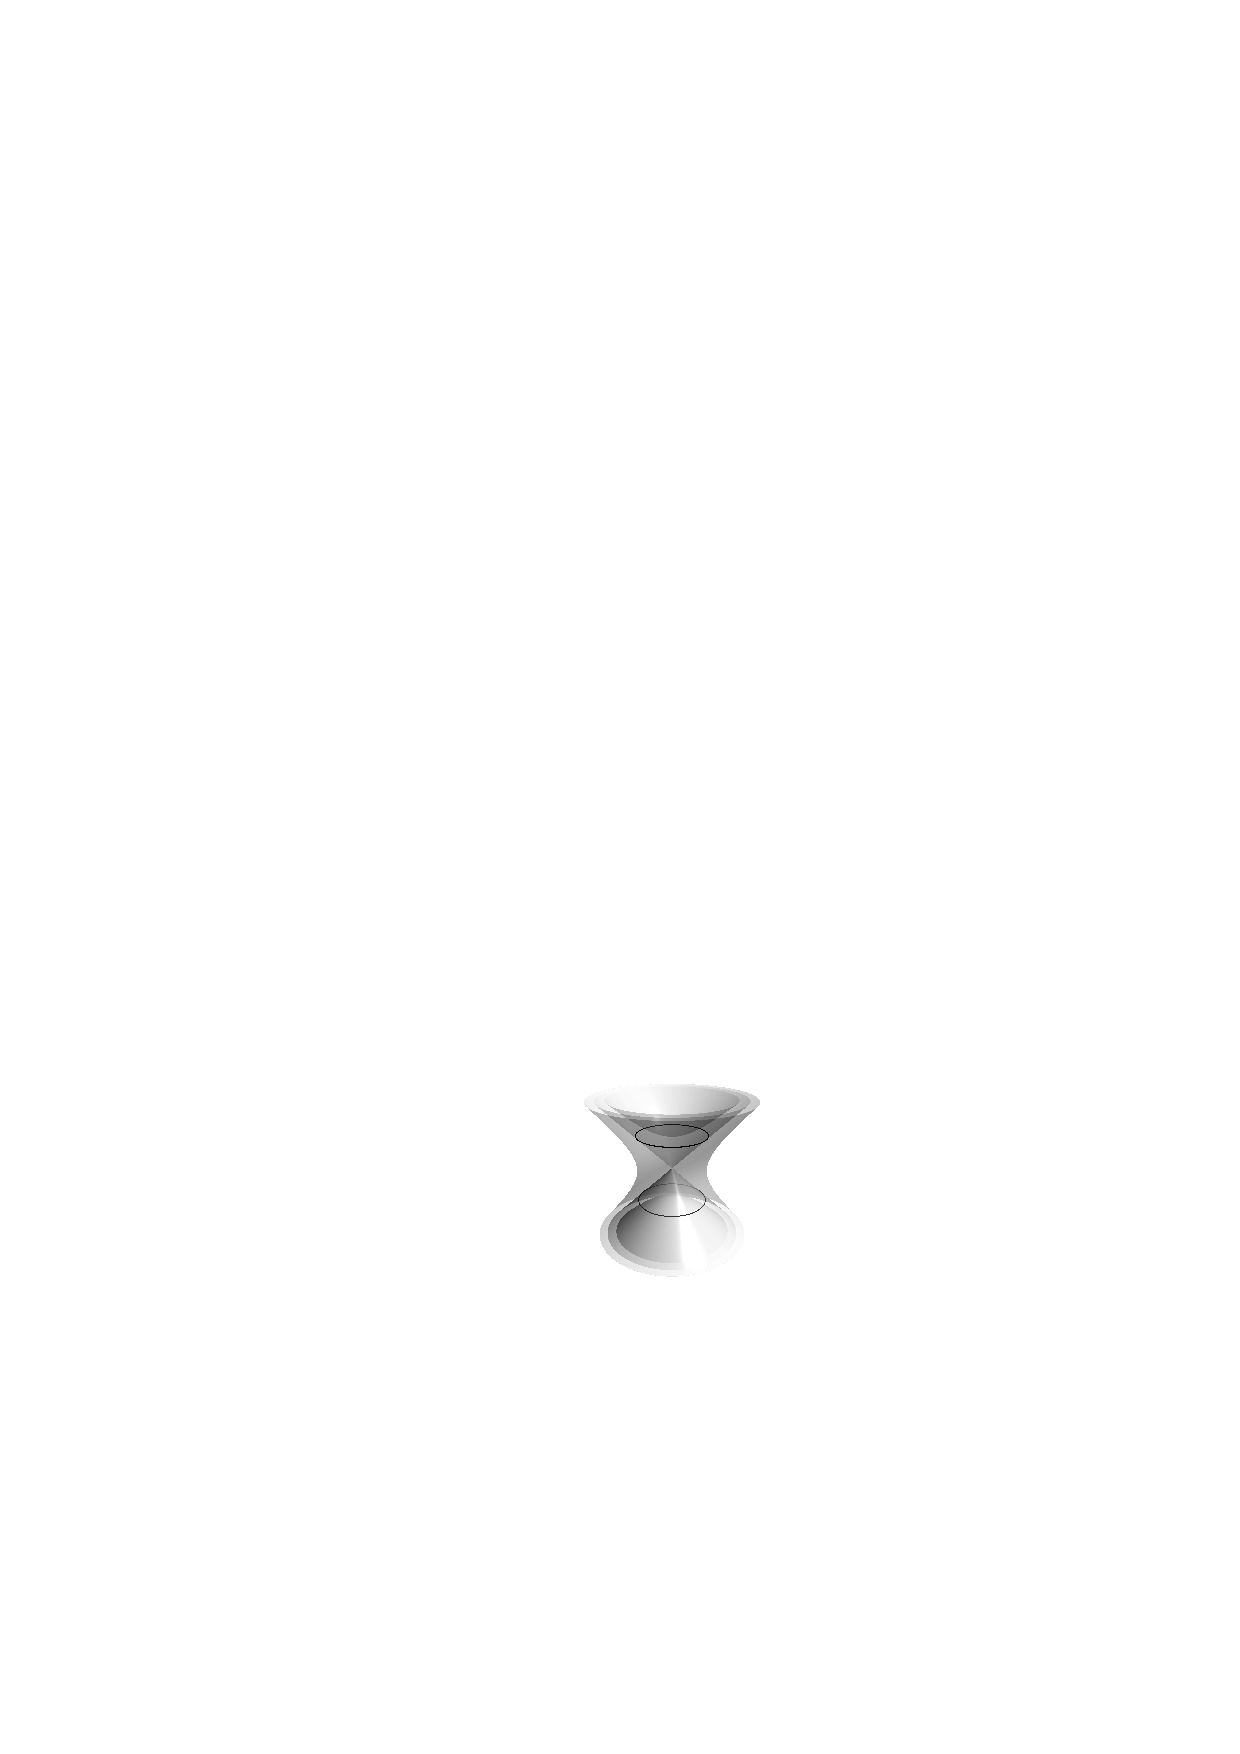
\includegraphics[scale=0.8]{figures/null cone.pdf}
    \caption{The set of unit null vectors within the null cone in signature $(1,2)$ (the $1$ corresponding to the vertical axis). \label{fig null cone}}
\end{figure}

We have the following obvious $\Or_V$-equivariant fiber bundles (the first two are covering maps)
\[\{\pm 1\}\hookrightarrow Y_\pm\to X_\pm,\quad \bbR^\times\hookrightarrow Y_0\to X_0,\]
while the following are $\CO_V$-equivariant fiber bundles:
\[\bbR^\times\hookrightarrow U_\pm\to X_\pm,\quad \bbR^\times\hookrightarrow Y_0\to X_0.\]
To see the diffeomorphism types of these manifolds, pick a space time splitting $V=V^+\oplus V^-$. Let $|x|=\sqrt{|\<x,x\>|}$ for $x\in V^+\cup V^-$. Let $S_+\subset V^+$, $S_-\subset V^-$ be the unit ``spheres'' $\lVert x\rVert =1$. Then each nonzero vector is uniquely decomposed as $x+y$ with $x\in V^+$, $y\in V^-$ and being null is equivalent to $|x|=|y|$. Scale the null vector to have $|x|=|y|=1$ and call it a \emph{unit null vector} (however, this is not a natural concept as it depends on the splitting). Then the set of unit null vectors is precisely $S_+\times S_-\subset Y_0$, see Figure~\ref{fig null cone}. Every nonzero null vector $x+y$ scales to a unit null vector, so 
\[Y_0\cong R_+\times S_+\times S_-,\]
and there is a double covering map 
\[\{\pm 1\}\hookrightarrow S_+\times S_-\to X_0\]
taking $x+y$ to the line spanned by $x+y$, so the null quadric $X_0$ is the quotient of the unit null vectors by the double antipodal map $x+y\mapsto (-x)+(-y)$. Note that $S_+\times S_-\subset V$ is not invariant under $\Or_V$ since it depends on the choice of splitting $V=V^+\oplus V^-$.

Every element of $Y_+$ splits uniquely into a sum $x+y$ with $x\in V^+$, $y\in V^-$ with $|x|^2=1+|y|^2>0$. There is a map 
\[Y_+\to S_+\times V^-,\quad x+y\mapsto (x/|x|,y),\]
and it can be inverted:
\[S_+\times V^-\to Y_+,\quad  (u,y)\mapsto \sqrt{1+|y|^2}u+y,\]
hence we have diffeomorphisms
\[Y_+\cong S_+\times V^-,\quad Y_-\cong V^+\times S_-.\]
Similarly, 
\[U_+\to \bbR^+\times S_+\times V^-,\quad x+y\mapsto (|x|,x/|x|,y)\]
is a diffeomorphism. 

As we will see later, every Lie group with finitely many components smoothly retracts to its maximal compact subgroup, and so every homogeneous space of that group retracts to the orbit of that maximal compact subgroup. So $\Or_{p,q}$ retracts to $\Or_p\times\Or_q$. In particular, $\Or_{p,q}$ has one component if $p=q=0$, two components if one of $p,q$ is zero, and four components otherwise.  As above, each of $Y_+,Y_-,Y_0$ retracts  $\Or_p\times\ \Or_q$-equivariantly to the orbits of $e_1^+,e_1^-,e_1^++e_1^-$, respectively, i.e., to $\bbS^{p-1}$, $\bbS^{q-1}$, $\bbS^{p-1}\times\bbS^{q-1}$. Here we note that $\bbS^{0}=\{\pm 1\}$ and $\bbS^{-1}=\varnothing$.

\textbf{Tangent spaces.} We can finally move on to describing the actual geometry. By differentiating the constant inner product we find that the tangent spaces of $Y_+,Y_-,Y_0$ at a point $x$ are identified with the hyperplane $x^\perp$ orthogonal to $x$:
\[\T_x Y=x^\perp\quad \text{for }x\in Y,\; Y=Y_+,Y_-,Y_0\]
Denote by $e^+_{2\ldots p}$ the list of vectors $e_2^+,\ldots,e^+_p$, etc. The various tangent spaces and stabilizers $H\coloneqq G_{x_0}$ are:
\begin{center}
    \begin{tabular}{l c c c r} 
     $Y$ & Basepoint $x_0$ & $\T_{x_0}Y$ & Signature of $Y$ & $H$\\ [0.5ex] 
     \hline
     $Y_+$ & $e_1^+$ & $\<e^+_{2\ldots p},e^-_{1\ldots q}\>$ & $(p-1,q)$ & $\Or_{p-1,q}$\\ 
     $Y_-$ & $e_1^-$ & $\<e^+_{1\ldots p},e^-_{2\ldots q}\>$ & $(p,q-1)$ & $\Or_{p,q-1}$\\ 
     $Y_0$ & $e_1^++e_1^-$ & $\<e^+_1-e^-_1,e^+_{2\ldots p},e^-_{2\ldots q}\>$ & $(p-1,q-1)$ & $\Or_{p-1,q-1}\times \bbR^\times$.\\
     \hline
    \end{tabular}
\end{center}

On each $\Or_{p,q}$-orbit, by $\Or_{p,q}$-invariance of the inner product, the signature of the restriction of the inner product to the orbit is the same at all points. Note that on $Y_0$, the inner product has a null direction, precisely the rescaling direction. Under the rescalings, the inner product recales, so $X_0$ inherits only a \emph{conformal metric} of signature $(p-1,q-1)$. When we quotient $Y_+,Y_-$ by $\pm\rmI$, we swap the choice of preimage of the resulting point in $X_+,X_-$, but we apply an orthogonal transformation which identifies the tangent spaces at the two points, so the resulting metric is defined on $X_+,X_-$. So $X_+$ has a smooth metric of signature $(p-1,q)$, while $X_-$ has a smooth metric of signature $(p,q-1)$, and $X_0$ has a smooth conformal structure of signature $(p-1,q-1)$. The orthogonal groups serve as stabilizers for $X_+,X_-$, so these metrics are invariant under automorphisms which act transitively on points and orthonormal frames, i.e., on orthonormal frame bundles. The stabilizers acting on $X_+,X_-$, as subgroups of $\CO_V=\Or_V\slash\{\pm\rmI\}$, are the isomorphic images of $\Or_{v^\perp}$ with $v=e_1^+,e_1^-$, respectively, as we can lift each transformation uniquely to have it fix $v$.

\textbf{Levi-Civita connection.} Each point $x\in Y=Y_\pm $ has normal space the span of $x$, and hence an orthogonal decomposition into tangent and normal spaces, $\T_x V=\T_x Y\oplus \rmN_x Y$ with $\rmN_x Y\coloneqq (\T_x Y)^\perp <\T_x V$. Given a curve $x(t)\in Y_\pm$, any vector field $v(x(t))\in V$ defined ``along the curve'' decomposes into tangent and normal parts. The derivative $\dot v(t)$ in the usual Euclidean sense splits into tangent and normal parts as well. If $v$ is everywhere tangent (normal), define $\nabla_{\dot x}v$ (resp., $\nabla_{\dot x}^\perp v$) to be the tangent (resp., normal) part of $\frac{\dd}{\dd t} v(x(t))$:
\[\frac{\dd}{\dd t} v(x(t))=\underbrace{\nabla_{\dot x}v}_{\T Y}+\underbrace{\nabla_{\dot x}^\perp v}_{\rmN Y}.\]  
Clearly, this definition is invariant under the orthogonal group. The value of $\nabla_{\dot x}v$, $\nabla_{\dot x}^\perp v$ at a point $t=t_0$ depends only on the vector $\dot x(t_0)$, the tangent vector $v(x(t_0))$, and its first derivative $\frac{\dd}{\dd t} v(x(t_0))$. Thus, they extend uniquely (via Willmore's Theorem as usual) to affine connections $\nabla,\nabla^\perp$ on $\T Y$ and $\rmN Y$, respectively.

\begin{xca}
    Show that the connection $\nabla$ is torsion-free and compatible with the metric $\sfg_\pm$ on $Y_\pm$ induced from the inner product on $V$, i.e., $\nabla\sfg_\pm=0$. Consequently, it is the Levi-Civita connection.
\end{xca}

By invariance under the orthogonal group, these connections also descend to $X_\pm$, and $\nabla$ is the Levi-Civita connection on $X_\pm$, too. Take a tangent vector $v\in \T_x Y_+$, which implies $v\perp x$. Let $P\coloneqq \<x,v\><V$ be the $2$-dimensional subspace through $x$ and $v$.  By applying an orthogonal transformation we can arrange that $x=e_1^+$ and $v$ is a multiple of either $e_2^+$ (if timelike) or $e_1^-$ (if spacelike). Hence, we can construct the linear reflection map fixing $x$ and $v$ and changing the signs of all other vectors in an orthonormal basis, i.e., a reflection fixing all points in $P$ and changing the signs of all points in $P^\perp$. The geodesic curvature of the curve $Y_+\cap P$, defined as the norm of the tangent component of its acceleration vector (cf.\ \ref{eq geodesic curvature}) is thus invariant under this reflection since the curve itself is, but at the same time lies in $P^\perp$ and hence must change sign. Thus, the curvature is zero and $Y_+\cap P$ is actually a geodesic. Similarly, if $v$ is null, we can arrange $v=e_2^++e_2^-$, and a change of the basis $e_2^+, e_2^-$ by a hyperbolic rotation $\left(\begin{smallmatrix}
    \cosh t & \sinh t\\\sinh t & \cosh t
\end{smallmatrix}\right)\in\Or_{1,1}$ (which are the only orthogonal transformations preserving $\<e_2^+, e_2^-\>$) scales $v$ by $\rme^t$ and the other null line in the plane $\<e_2^+, e_2^-\>$  by $\rme^{-t}$. Hence, the curvature is invariant and thus vanishes -- a geodesic. Similarly for $Y_-$. 

This gives one geodesic in each direction, so we have all of the geodesics: a curve on $Y_\pm$ is a geodesic iff, at some point, it is the intersection with a plane containing the normal vector at that point. Mapping to projective space, the geodesics on $X_\pm$ are its intersection with projective lines.

\begin{example}
    In $\bbR^{1,2}$, the surface $Y_+$ is the two-sheeted hyperboloid $x^2+y^2+1=z^2$ with a Riemannian metric invariant under the orthogonal (Lorentz) group $\Or_{1,2}$. The vertical plane through $\bf{e}_1^+$ intersects the cone at two points, so the geodesic is the hyperbola in between. All the geodesics in $Y_+$ are carried to one another by isometries, so the action on geodesics in $Y_+$ is transitive.

    The surface $Y_-$ is the one-sheeted hyperboloid $x^2+y^2=1+z^2$. Every point $\bf{x}\in Y_-$ can be brought to the point $\bf{e}_1^-$ by an orthogonal transformation. The horizontal $(x,y)$-plane $\<\bf{e}_1^-,\bf{e}_2^-\>$ intersects $Y_-$ along a spacelike geodesic circle. The planes $\<\bf{e}_1^-,\pm \bf{e}_1^++\bf{e}_1^-\>$ intersect $Y_-$ along null geodesics -- the lines $x=\pm 1$. All pointed geodesics are carried to one of these by orthogonal transformations, so there are two orbits on the space of geodesics in $Y_-$.
\end{example}

\textbf{dS and AdS.} We now name and describe the isometry groups of the three geometries $X_+,X_-,X_0$, starting with the first two.

\begin{defn}\index{de Sitter space}\index{anti-de Sitter space}\index{dS!see {de Sitter space}}\index{AdS!see {Anti-de Sitter space}}
    The de Sitter space $\mathrm{dS}^{p-1,q}$ and the anti-de Sitter space $\mathrm{dS}^{p,q-1}$ of dimension $p+q-1$ are defined as the projective images $X_+$ and $X_-$ in $\RP^{p+q}$, respectively, of the unit hyperboloids $Y_+,Y_-$ inside $\bbR^{p,q}$, with their induced pseudo-Riemannian structures, as described above.
\end{defn}

\begin{thm}
    The group of pseudo-Riemannian isometries of the de Sitter space $X_+$ and anti-de Sitter space $X_-$ is precisely the projective orthogonal group $G=\Or_{p,q}\slash\{\pm \rmI\}$.
\end{thm}
\begin{proof}
    The projective orthogonal group acts transitively. Consider the stabilizer of a point. Looking at our description of tangent spaces above, the stabilizer of a point acts transitively on orthogonal frames at that point, i.e., as the orthogonal group of that tangent space. Take any isometry. Composing it with an element of $G$, we can arrange that it fixes a given point $x_0$, and a frame at that point, i.e., acts trivially on the tangent space  $\T_{x_0} X$ at that point. Since any isometry takes geodesics to geodesics, this map commutes with the exponential map $\exp_{x_0}:\T_{x_0} X\to X$ (defined as the value at time $t=1$ of the geodesic starting at $x_0$ with given velocity). We will later see that $\exp_{x_0}$ is a local diffeomorphism and hence our isometry fixes an entire open neighborhood. By analyticity and connectivity (uniqueness of analytic continuation), this isometry must be the identity map.
\end{proof}

We thus have the description of dS and AdS as the following homogeneous spaces (we add the signatures to the notation for clarity):
\begin{gather}
    \{\pm 1\}\hookrightarrow Y_+^{p-1,q}\cong \bbS^{p-1}\times\bbR^q\cong \Or_{p,q}\slash \Or_{p-1,q}\to X_+^{p-1,q},\\
    \{\pm 1\}\hookrightarrow Y_-^{p,q-1}\cong \bbR^p\times \bbS^{q-1}\cong \Or_{p,q}\slash \Or_{p,q-1}\to X_-^{p,q-1},
\end{gather}
where the last covering map in both cases is the quotient map by the antipodal identification $x\sim -x$. In the standard physics terminology, $\mathrm{dS}^n=X_-^{1,n-1}$ and $\mathrm{AdS}^n=X_+^{1,n-1}$. Note that the space $\bbS^1\times\bbR$ corresponding to $n=2$ carries simultaneously a de Sitter and an anti-de Sitter geometry (the same more generally holds for $\bbS^p\times\bbR^p$). 

\textbf{Null quadric.} The description of the stabilizer of a point of the null quadric $X_0$ is more complicated. First let us change the variables of our standard example to get the axes of the first and last coordinates to be null, so $V=\bbR\oplus V'\oplus \bbR$ with $V'$ of signature $(p-1,q-1)$. If we denote these two so called \emph{light cone coordinates} by $x^+$ and $x^-$ (in no particular order) then this means that the metric contains the term $x^+x^-$. We would like to describe the isometries of $V$ that stabilize a given point of $X_0$, and these obviously map to some subgroups of the groups described in Lemma~\ref{lem null quadric isometries}.

First we can eliminate one complication related to the split case. If the signature is split, then so is that of $V'$; in the split case, take a conformal transformation $T'\in\CO_{V'}$ changing the sign of the inner product (this exists by induction starting with $(x^1,x^2)\mapsto (x^2,x^1)$ for $p=q=1$) and let 
\[T\coloneqq \begin{pmatrix}
    1 & 0 & 0\\
    0 & T' & 0\\
    0 & 0 & -1
\end{pmatrix},\]
so that $T$ changes the sign of the inner product and fixes the standard basis vector $\bf{e}_1$. This $T$ is exactly the $T$ that generates the extra components of the split isometry groups of the null quadric in Lemma~\ref{lem null quadric isometries}. Since it stabilizes $\bf{e}_1$, it will be included in the stabilizer and thus can be effectively ignored in the description of $X_0$ as a homogeneous space.

It remains to describe the isometric part of the stabilizer of $\<\bf{e}_1\>\in X_0$. Let $P_O\subset \Or_V$ and  $P_C\subset \CO_V$ be, respectively, the groups of orthogonal and conformal transformations which stabilize the null line $\<\bf{e}_1\>$ in these coordinates.

\begin{lem}
    In the above basis, the group $P_O$ consists precisely of the matrices of the form 
    \[g=\begin{pmatrix}
        a & av^\flat h & \frac{a}{2}\<v,v\>\\
        0 & h & v \\
        0 & 0 & a^{-1}
    \end{pmatrix},\]
    where $a\in \bbR^\times$, $v\in V'$, $h\in \Or_{V'}$, $v^\flat\coloneqq \sfg(v)\in (V')^\ast$ the dual covector w.r.t.\ the inner product $\sfg\in \Hom(V,V^\ast)$.  The group $P_C$ consists of matrices of the form $\lambda g$, where $\lambda>0$ and $g\in P_O$.
\end{lem}
\begin{proof}
    We assume a basis as above. After a positive scaling, these conformal transformations are orthogonal transformations. So assume that $g$ is orthogonal and preserves the line spanned by the null vector $\bf{e}_1$, and so preserves the perpendicular space of that vector, which is the span of the entire standard basis minus the \emph{last} vector $\bf{e}_{p+q}$. Hence, $g$ has the form 
    \[g=\begin{pmatrix}
        a & \xi & t\\
        0 & h & v\\
        0 & 0 & b
    \end{pmatrix}\]
    for some $a,b\in \bbR^\times$, $h\in \GL_{V'}$, $v\in V'$, $\xi\in (V')^\ast$.

    Write the inner product on $V'$ as $\<v,w\>=\<v,\eta w\>_{\mathrm{Euc}}$, where $\<\,,\,\>_{\mathrm{Euc}}$ is the regular dot product on $\bbR^{p+q-2}$ in our fixed basis, and $\eta$ is some symmetric matrix of signature $(p-1,q-1)$. Let 
    \[S\coloneqq \begin{pmatrix}
        0 & 0 & -1\\
        0 & \eta & 0 \\
        -1 & 0 & 0
    \end{pmatrix}.\]
    Since $g$ is an isometry and $S$ is nothing but the metric tensor written in the basis where $\bf{e}_1,\bf{e}_{p+q}$ were replaced by $\bf{e}_1\pm \bf{e}_{p+q}$, we must have $g^T Sg=S$, which forces $g$ to have the asserted form.
\end{proof}

Thus, $X_0^{p-1,q-1}\coloneqq X_0$ is a conformal manifold of signature $(p-1,q-1)$ obtained as the homogeneous space 
\[\{\pm 1\}\hookrightarrow \bbS^p\times\bbS^q\to X_0^{p-1,q-1}=\CO_{p,q}\slash P_C=\Or_{p,q}\slash P_O.\]
Lastly, we note the obvious isomorphisms under swapping the sign of the entire metric on $V$: $X_+^{p,q}\cong X_-^{q,p}$ and $X_0^{p,q}\cong X_0^{q,p}$.










\chapter{Cartan Geometry}\label{ch: cartan geom}


Our encounter with geometric structures on manifolds started with Lie groups, in which we saw that the Maurer-Cartan equation provided the basis for the entire Lie group structure, and hence the theory of Lie groups. Then, separately, we developed the theory of principal connections and saw that the structure equation for the curvature is very reminiscent of the Maurer-Cartan equation, thus suggesting that all connections are, in some way, ``deformations'' of canonical geometries on Lie groups and their homogeneous spaces. Nevertheless, the Maurer-Cartan form itself couldn't exactly be interpreted as neither a connection form nor a soldering form. It is very close to being a soldering form in its relation to the torsion of canonical flat connections (Example~\ref{ex connections on G, part 6}), whereas the only way to turn it into a principal connection is to project it onto a Lie subalgebra in a reductive Klein geometry (Example~\ref{ex 1.3.19 RS2}). Cartan geometry will finally unify these approaches, allow us to intepret the Maurer-Cartan form as a fundamental example of a general geometric structure, and all other geometric structures that we've seen so far as ``deformations'' of the ``model structures'' of Klein geometries. In this picture, we may succinctly describe all of modern differential geometry as a vast generalization of the Maurer-Cartan equation.






\section{Cartan connections}

Any Cartan geometry is derived from a homogeneous space, called the homogeneous model of the geometry. The interplay between this homogeneous model and general Cartan geometries of the given type is one of the main general features of Cartan geometries and an important topic for this section.


\begin{defn}[Cartan geometry I]\index{Cartan geometry}\index{Connection!Cartan}\label{def cartan geometry I}
    Then a \emph{Cartan geometry of type $(G,H)$ on a manifold $M$} is a tuple $(P\overset{\pi}{\to}M,G,H,\Phi,\eta)$, where $(G,H)$ is a Klein geometry (i.e., $H\emb G$ is a closed subgroup of a Lie group $G$ such that $G\slash H$ is connected),
    $(P\overset{\pi}{\to}M,H,\Phi)$ a principal $H$-bundle, and $\eta\in\Omega^1(P;\frakg)$ is a $\frakg$-valued $1$-form, called the \emph{Cartan connection}, which is required to be $H$-equivariant, to reproduce the generators of Killing vector fields, and to define an absolute parallelism on $P$. More formally,
    \begin{enumerate}
        \item $\Phi_h^\ast \eta=\Ad_h^{-1}\circ \eta$ for all $h\in H$;
        \item $\eta(A_\ast(p))=A$ for all $A\in\frakh$ and $p\in P$;
        \item (Cartan condition) $\ker\eta_p=0$ (hence $\eta_p$ is a linear isomorphism) for all $p\in P$, i.e., $\eta$ determines an absolute parallelism presented by the bundle isomorphism $\eta:\T P\to P\times\frakg$.
    \end{enumerate}
    The \emph{homogeneous model} for Cartan geometries of type $(G,H)$ is the canonical Klein geometry (homogeneous principal $H$-bundle) $G\to G\slash H$ endowed with the left Maurer-Cartan form $\theta_G\in\Omega^1(G;\frakg)$.

    Given a Cartan geometry, the \emph{constant vector fields} are $\eta^{-1}(A)\in\fX(P)$ defined for all $A\in\frakg$ by $\eta(\eta^{-1}(A)_p)=A$ at any $p\in P$. Projections of integral curves of constant vector fields to $M$ are called \emph{spirals}, \emph{generalized circles}, or \emph{canonical curves}. The Cartan connection $\eta$ is called \emph{complete} if all of its constant vector fields are complete.
\end{defn}

We will often use the simplified notation $p\cdot h$ for $\Phi_h(p)$. By equivariance of $\eta$, we get the transformation rule for constant vector fields
\[\eta^{-1}(A)_{p\cdot h}=\Phi_{h\ast}\circ \eta^{-1}(\Ad_h A)_p,\quad \text{for all}\quad h\in H.\]


\begin{example}
    In the case of the homogeneous model, the constant vector field $\theta_G^{-1}(A)$ is the left-invariant vector field $A_\rmL$. Moreover, the pullback of $\eta$ along the orbit map $\Phi^p:H\to P_{\pi(p)}$ (which is a diffeomorphism) is exactly the Maurer-Cartan form $\theta_H$. Restrictions of the homogeneous model to an open subset $U\subset G\slash H$ are also flat Cartan geometries. If $U$ is not simply connected, then all of its covering spaces also carry an induced flat Cartan structure.
    % These forms define a global $1$-form on the vertical bundle, $\theta_H:\calV P\to \frakh$, which can be viewed as a global trivialization $\calV P\to P\times\frakh$.
     Thus, general Cartan geometries of type $(G,H)$ are seen as ``curved analogs'' of the Klein geometry $(G,H)$, with the Maurer-Cartan form $\theta_G$ replaced by the Cartan connection form.
\end{example}

\begin{example}
    The next simplest examples are locally Klein geometries $G\to \varGamma\bslash G\slash H$, where $\varGamma<G$ is a discrete subgroup that acts on $G\slash H$ by left translations. Then $\varGamma$ acts on $G$ by deck transformations and hence isomorphisms of the Cartan geometry. Since $G\to \varGamma\bslash G$ is a covering map, it is a local diffeomorphism, and we can push the Cartan structure forward to the $H$-bundle $\varGamma\bslash G \to \varGamma\bslash G\slash H$. This is still a flat Cartan geometry.
\end{example}


\begin{defn}[Curvature form of a Cartan geometry]\index{Curvature!of a Cartan geometry}
    The curvature form $\Omega\in\Omega^2(P;\frakg)$ of a Cartan geometry $(P\to M,G,H,\Phi,\eta)$ is defined by the structure equation 
    \[\Omega(X,Y)\coloneqq \dd\eta(X,Y)+[\eta(X),\eta(Y)].\]
\end{defn}


\begin{example}
    \begin{enumerate}
        \item The Maurer-Cartan equation implies that Klein geometries $(G,H)$ with their \emph{canonical Cartan connections} given by the Maurer-Cartan form are always flat. This is why the homogeneous model is often referred to as the flat model, although we avoid this terminology due to the likely confusion with flat principal connections. Indeed, by dimension counting, a Cartan connection is a principal connection only in the case of the trivial Klein geometry $(G,G)$ consisting of a single fiber.
        \item Cartan geometries, therefore, are \emph{not} a generalization of principal connections. And although Cartan connections can be viewed as a special class of principal connections by changing the underlying bundle (see the next \sect), in fact, these concepts are almost orthogonal in a sense that will be clarified below.
        \item If $\eta$ is a Cartan connection of type $(G,H)$ on $P$ and $B\emb H$ is a closed subgroup, then $\eta$ defines a Cartan connection of type $(G,B)$ on $P\to P\slash B= P\times^H (H\slash B)$.\label{xca V.3.6 Sharpe}
    \end{enumerate}
\end{example}


Since the Cartan conection $\eta$ trivializes $\T P$, any differential form on $P$ is determined by its values on the constant vector fields $\eta^{-1}(A)$. Thus, the complete information about $\Omega$ is contained in the \emph{curvature function}\index{Curvature!Function} $\scrK:P\to \bigwedge\nolimits^2\frakg^\ast\otimes\frakg$ defined by 
\[\scrK_p(A,B)=\Omega_p\left(\eta^{-1}(A),\eta^{-1}(B)\right),\]
and then the standard formula for the exterior derivative yields 
\[\scrK_p(A,B)=[A,B]-\eta_p\left(\left[\eta^{-1}(A),\eta^{-1}(B)\right]\right).\]
In other words, curvature measures the failure of the assignment of the constant vector fields $A\mapsto \eta^{-1}(A)$ to be a homomorphism of Lie algebras $\frakg\to \fX(P)$.

\begin{lem}[{{\cite[Lem.~1.5.1]{Cap}}}]\label{lem 1.5.1 Cap}
    The curvature form $\Omega\in\Omega^2(P;\frakg)$ is horizontal, so the curvature function may be viewed as $\scrK:P\to \bigwedge\nolimits^2(\frakg\slash\frakh)^\ast\otimes\frakg$. Moreover, $\Omega$ is \emph{of type $\Ad$ w.r.t.\ $H$} in the sense that 
    \begin{align}
        \Phi_h^\ast \Omega&=\Ad_h^{-1}\circ \Omega,\\
        \Phi_h^\ast\scrK&=\lambda(h)^{-1}\circ\scrK,
    \end{align}
    where $\lambda$ is the tensor product of the actions $\bigwedge\nolimits^2 \underline{\Ad}^\ast$ on $\bigwedge\nolimits^2(\frakg\slash\frakh)^\ast$ and $\Ad$ on $\frakg$.
\end{lem}
\begin{proof}
    By definition of $\eta$, if $A\in\frakh$, then $\eta^{-1}(A)=A_\ast$, the Killing vector field. Equivariance of $\eta$ implies that $\Lie_{A_\ast}\eta=i_{A_\ast}\dd\eta=-\ad_A\circ\eta$. This gives 
    \[\dd\eta(\eta^{-1}(A),Y)+[A,\eta(Y)]=-\ad_{A}\eta(Y)+[A,\eta(Y)]=0\]
    for all $A\in\frakh$ and all $Y\in \T P$. Since the Killing vector fields span the vertical bundle, we conclude that $\Omega$ is horizontal, and that each $\scrK_p$ descends to $\bigwedge\nolimits^2(\frakg\slash\frakh)$.
    
    The equivariance property of $\Omega$ follows directly from the definition and the naturality of $\dd$ w.r.t.\ pullbacks. To prove the property for $\scrK$, we have to compute $\scrK_{p\cdot h}(X,Y)$. By definition, we find 
    \begin{align}
        \Omega\left(\eta_{p\cdot h}^{-1}(A),\eta_{p\cdot h}^{-1}(B)\right)&=\Omega\left(\Phi_{h\ast}\eta^{-1}_p(\Ad_h A),\Phi_{h\ast}\eta^{-1}_p(\Ad_h B)\right)=\notag\\
        &=(\Phi_h^\ast \Omega)_p \left(\eta^{-1}(\Ad_h A),\eta^{-1}(\Ad_h B)\right)=\notag\\
        &=\Ad_h^{-1}\scrK_p(\Ad_h A,\Ad_h B).
    \end{align}
    Passing from $\frakg$ to $\frakg\slash\frakh$, the two occurrences of $\Ad_h$ inside of $\scrK_p$ are replaced by $\underline{\Ad}_h$, and we obtain the asserted formula.
\end{proof}



\begin{example}\label{ex 1.5.1 Cap}
    \begin{enumerate}[label=(\roman*)]
        \item Let $\Aff_n(\bbR)$ be the affine group in dimension $n$. We have seen in Remark~\ref{rem 1.3.6 Cap} that a Cartan geometry of type $(\Aff_n(\bbR),\GL_n(\bbR))$ on an $n$-dimensional manifold $M$ is equivalent to a linear (affine) connection $\omega$ on the frame bundle $\Fr(\T M)$. Moreover, the curvature $\Omega$ coincides with the sum $\Omega+\Theta$ of the curvature and the torsion of that linear connection. The Cartan connection is $\eta=\omega+\theta$, where $\theta$ is the soldering form.
        \item For a Lie group $H$ and an infinitesimally injective homomorphism $H\to \GL_n(\bbR)$ consider the affine extension $B=\bbR^n\rtimes H$. In  we saw that a Cartan geometry of type $(B,H)$ is equivalent to a first-order $G$-structure with structure group $H$ endowed with a connection. The curvature of the Cartan connection can again be interpreted as the direct sum of the curvature and torsion of the induced affine connection on the tangent bundle.
        \item More specifically, consider $H=\Or_n\emb \GL_n(\bbR)$. Then the affine extension $\bbR^n\rtimes H$ is the Euclidean group $\SE_n$. By Example~\ref{ex pseudo-riemannian structure} an $\Or_n$-structure is equivalent to a Riemannian metric $\sfg$ on $M$. From (ii) we thus conclude that a Cartan geometry of type $(\SE_n,\Or_n)$ is equivalent to a connection on the orthonormal frame bundle for $\sfg$ and hence to a unique metric affine connection on $\T M$. The Levi-Civita connection then gives a canonical Cartan geometry of type $(\SE_n,\Or_n)$ on each Riemannian manifold. The curvature then effectively coincides with the usual Riemann curvature, since the torsion vanishes.
        
        This is a prototypical example for a Cartan geometry which is determined by an underlying structure. The interpretation of Riemannian structures as Cartan geometries is one of the motivating examples for the concept. 
        \item There is no difference between Cartan geometries of the types $(\Or_{n+1},\Or_n)$, $(\SE_n,\Or_n)$, and $(\Or_{1,n},\Or_n)$. This is because $\frako_{n+1}$, $\frakse_{n}$, and $\frako_{1,n}$ are all isomorphic as $\Or_n$-modules. However, the notion of curvature is different for these three types of geometries, since the homogeneous models $\bbS^n$ (Riemann sphere) and $H^n$ (hyperbolic space) of the first and last types have (nonzero) constant curvature unlike the second type. This is an example of model \emph{mutation}, which we will discuss in detail below.
    \end{enumerate}
\end{example}

\begin{example}[Product of Cartan geometries]
    On the product of two unit $2$-spheres, $M=\bbS^2\times\bbS^2$, the Cartan geometry obtained as the bundle product $P\times P\to M$ of their respective Riemannian geometries is \emph{not} the product Riemannian geomery. The Cartan geometry keeps track of the order of the product and has structure group $\Or_2\times\Or_2$, while the Riemannian geometry has the permutation of the factors as an isometry and has structure group $\Or_4$.
\end{example}

\begin{example}[\ref{ex dS and AdS} continued]\label{ex dS and AdS 2}
    Recall that the de Sitter and anti-de Sitter spaces are, respectively, $\mathrm{dS}^n=\Or_{1,n}\slash \Or_{1,n-1}$ and $\mathrm{AdS}^n=\Or_{2,n-1}\slash \Or_{1,n-1}$. This means that the isometry groups of these spaces are $\Or_{1,n}$ and $\Or_{2,n-1}$, respectively, whereas the structure group is $\Or_{1,n-1}$, so both geometries are \emph{Lorentz manifolds} \index{Lorentz manifold} (that is, pseudo-Riemannian manifolds of signature containing only one minus). In cosmology, the $4$-dimensional $\mathrm{dS}^4$ and $\mathrm{AdS}^4$ are the basic models for the global geometry of the ``static universe.''

    In the case of $\mathrm{dS}^3$, one can extend the symmetry group to $G=\SL_2(\bbC)\cong\Spin_{1,3}$, which is the universal covering group of the Lorentz group $\SO^+_{1,3}$ (the identity component of $\Or_{1,3}$). Then the stabilizer of a point is $\SL_2(\bbR)\cong \Spin_{1,2}$, so 
    \[\mathrm{dS}^3\cong \SL_2(\bbC)\slash\SL_2(\bbR)\cong \Spin_{1,3}\slash \Spin_{1,2}.\]
    Similarly, one can identify $\mathrm{AdS}^n\cong \Spin^+_{2,n-1}\slash \Spin^+_{1,n-1}$.
\end{example}

\begin{example}
    All common types of differential geometries are covered by Cartan geometry. Projective geometries are geometries modeled on $\RP^n$ or $\CP^n$ with $G$ their respective projective linear group $\PSL_{n+1}(\bbR)$ or $\PSL_{n+1}(\bbC)$, and projective connections are Cartan connections of this type (which can be also required to be holomorphic in the complex case). A spin connection is a Cartan geometry of type $(\Spin_n\ltimes\bbR^n,\Spin_n)$. A symplectic connection is a Cartan geometry of type $(\Sp_n(\bbR)\ltimes\bbR^n,\Sp_n(\bbR))$ (these arise naturally in formal deformation quantization). A conformal connection is a Cartan geometry modeled on the conformal sphere. A CR structure is a Cartan geometry modeled on the CR sphere with $G=\PSU_{p+1,q+1}$.
\end{example}

\begin{defn}[Morphism of Cartan geometries]
    A morphism between two Cartan geometries $(P\to M,G,H,\Phi,\eta)$ and $(P'\to M',G,H,\Phi',\eta') $ of type $(G,H)$ is a principal bundle morphism $\vartheta:P\to P'$ such that $\vartheta^\ast\eta '=\eta$. Notice that compatibility with the Cartan connection implies that any tangent map of $\vartheta$ is a linear isomorphism, so $\vartheta$ and its base map are local diffeomorphisms. The resulting category of Cartan geometries of type $(G,H)$ is denoted $\Car_{(G,H)}$.
\end{defn}

\begin{lem}[{{\cite[Lem.~1.5.2]{Cap}}}]\label{lem 1.5.2 Cap}
    Let $\vartheta:P\to P'$ be a morphism of \glspl{pfb} which is a local diffeomorphism. If $\eta'$ is a Cartan connection on $P'$, then $\eta=\vartheta^\ast\eta'$ is a Cartan connection on $P$. If $\eta'$ and $\eta$ are fixed Cartan connections on $P$ and $P'$, then $\vartheta$ is a morphism of Cartan geometries iff it preserves the constant vector fields, i.e., $\vartheta_\ast\circ \eta^{-1}(A)=\eta^{\prime-1}(A)\circ\vartheta$. In this case the curvature forms $\Omega$ and $\Omega'$ (or $\scrK$ and $\scrK'$) are $\vartheta^\ast$-related.
\end{lem}
\begin{proof}
    The Killing vector fields are given by $A_\ast(p)=\restr{\frac{\dd}{\dd t}}{0}p\cdot \rme^{tA}$, so equivariance of $\vartheta$ implies that $\vartheta^\ast \eta'$ reproduces the generators of Killing fields. Similarly, equivariance of $\vartheta$ and $\eta'$ implies equivariance of $\vartheta^\ast\eta'$. Since $\vartheta$ is a local diffeomorphism, $\vartheta^\ast\eta'=\eta'\circ \vartheta_\ast$ restricts to a linear isomorphism on each tangent space, so we have verified that $\vartheta^\ast\eta'$ is a Cartan connection.

    The pullback $\vartheta^\ast\eta'$ evaluates on a constant field as 
    \[\vartheta^\ast\eta'(\eta^{-1}(A)_p)=\eta'(\vartheta(p))\left(\vartheta_{\ast p}\eta^{-1}(A)_p\right)\]
    and the right hand side equals $A$ iff $\vartheta_\ast\circ \eta^{-1}(A)_p=\eta^{\prime-1}(A)(\vartheta(p))$. Thus, morphisms morphisms are characterized by the fact that they preserve the constant fields. The relatedness of the curvature forms follows immediately from their definition via the structure equation. Finally, the relation between $\Omega$ and $\Omega'$ implies 
    \begin{align}
        \scrK_p(A,B)&=\Omega_p\left(\eta^{-1}(A),\eta^{-1}(B)\right)=\Omega'_{\vartheta(p)}\left(\eta^{\prime-1}(A),\eta^{\prime-1}(B)\right)=\notag
        \\&=\scrK'_{\vartheta(p)}(A,B)
    \end{align}
    for all $p\in P, A,B\in\frakg$.
\end{proof}


Various useful subcategories in $\Car_{(G,H)}$ can be defined by restrictions on curvature. Such restrictions are usually necessary to characterize Cartan geometries that are equivalent to simpler structures. The simplest way to restrict curvatures is by requiring the curvature function $\scrK$ to have values in a fixed subspace $\frakM\subset \bigwedge\nolimits^2(\frakg\slash\frakh)^\ast\otimes\frakg$. The simple transformation law $\scrK=\scrK'\circ \vartheta$ immediately implies that this specifies a full subcategory in $\Car_{(G,H)}$. However, as we have seen, $\scrK(p\cdot g)=g^{-1}\cdot \scrK(p)$, so the values of $\scrK$ always span an $H$-invariant subset in $\bigwedge\nolimits^2(\frakg\slash\frakh)^2\otimes\frakg$. Thus, it is natural to require that $\frakM$ is an $H$-submodule. 

\begin{defn}[$\Car_{(G,H)}^\frakM$]\label{def category of cartan geom}
    Consider the category $\Car_{(G,H)}$. If $\frakM\subset \bigwedge\nolimits^2(\frakg\slash\frakh)^\ast\otimes\frakg$ is an $H$-submodule, then we denote the full subcategory of Cartan geometries whose curvature functions take values in $\frakM$ by $\Car_{(G,H)}^\frakM$.

    In particular, if $\frakM=0$, such Cartan geometries are called \emph{locally flat}, and if $\frakM=\bigwedge\nolimits^2(\frakg\slash\frakh)^\ast\otimes\frakh$, then they are called \emph{torsion-free}. Finally, if $\frakM=\Hom_\frakh(\bigwedge\nolimits^2(\frakg\slash\frakh), \frakh)$, i.e., the set of $\ad(\frakh)$-invariants, then we say the geometry has \emph{constant curvature}.
\end{defn}

More generally, the \emph{torsion} of a Cartan geometry is the composition of its curvature function with the quotient map $\frakg\to \frakg\slash\frakh$. Only in reductive geometries, where there is a chosen decomposition of $H$-modules $\frakg=\frakh\oplus\frakm$, torsion can be seen as a literal ``component'' of curvature.

\begin{example}
    When $H$ is compact, it is known from representation theory of Lie groups that $(\frakg\slash\frakh)^\ast\otimes\frakh$ decomposes into a direct sum of irreducible representations of $H$. Each irreducible component defines ``a component of curvature''. For example, in the Riemannian case it splits into three components, corresponding to the scalar, the Ricci, and the Weyl curvatures.\index{Curvature!Weyl}\index{Curvature!Ricci} In dimension $4$, the Weyl curvature further splits into a self-dual and an anti-self-dual part. If $H$ is noncompact, then a decomposition into irreducibles may not be possible, but it may still contain submodules worth examining. For example, the composite mapping 
    \begin{align}
        \bigwedge\nolimits^2(\frakg\slash\frakh)^\ast\otimes\frakh\overset{\id\otimes \ad}{\to}&\bigwedge\nolimits^2(\frakg\slash\frakh)^\ast\otimes\End(\frakg\slash\frakh)\cong \notag\\
        \cong &\underset{t^\ast\wedge u^\ast\otimes v\otimes w^\ast}{\bigwedge\nolimits^2(\frakg\slash\frakh)^\ast\otimes(\frakg\slash\frakh)\otimes (\frakg\slash\frakh)^\ast}
        \underset{\mapsto}{\to} \underset{(t^\ast(v)u^\ast-u^\ast(v)t^\ast)\otimes w^\ast}{(\frakg\slash\frakh)^\ast\otimes (\frakg\slash\frakh)^\ast}
    \end{align}
    is $H$-equivariant, and hence its kernel is an $H$-submodule, called the \emph{normal submodule}. It is indirectly related to normal Cartan geometries, which are defined so that the Cartan geometry is uniquely determined by a set of geometric data that at the outset have no necessary relation to Cartan geometry, but determine one via Cartan's method of equivalence.
\end{example}

The reason for the naming of torsion-free geometries should be self-evident based on the examples of connections on $G$-structures that we saw. The name for locally flat geometries will be explained after the next proposition.

Since the homogeneous model $(G,H)$ will usually be fixed, we will often abbreviate the notation for a Cartan geometry $(P\overset{\pi}{\to} M,G,H,\Phi,\eta)$ by writing $(P\to M,\eta)$. Note that for any Cartan geometry $(P\to M,\eta)$ and an open subset $U\subset M$ there is a canonical Cartan geometry $\left(\restr{P}{U}\to U,\restr{\eta}{P|_U}\right)$, so one may restrict Cartan geometries to open subsets. We also reiterate two related statements about Klein geometries proven earlier.

\begin{prop}[{{\cite[Prop.~1.5.2]{Cap}}}]\label{prop 1.5.2 Cap}
    \begin{enumerate}[label=(\arabic*)]
        \item The curvature of a Cartan geometry $(P\to M,\eta)$ of type $(G,H)$ vanishes identically iff every $m\in M$ has an open neighborhood $U$ such that its restriction to $U$ is isomorphic to the restriction of the homogeneous model $(G\to G\slash H,\theta_G)$ to an open neighborhood of $[e]$.
        \item If $G\slash H$ is connected, then the automorphisms of the homogeneous Cartan geometry $(G\to G\slash H,\theta_G)$ are exactly the left translations $\rmL_g$, $g\in G$.
        \item (Liouville Theorem) Suppose that $G\slash H$ is connected. Then any isomorphism between two restrictions of $(G\to G\slash H,\theta_G)$ to connected open subsets of $G\slash H$ uniquely extends to an automorphism of the homogeneous model.
    \end{enumerate}
\end{prop}
\begin{proof}
    (1) Assume that the curvature vanishes. Then the Fundamental Theorem~\ref{thm 6.1 Sharpe fundamental local} implies that for each $p\in P$, there is a neighborhood $V$ of $p$ in $P$ and a unique map $\varphi:V\to G$ such that $\varphi(p)=e$ and $\varphi^\ast\theta_G=\eta$. In particular, $\varphi$ respects the constant fields restricted to $V$. This implies that for each $q\in V$, $\varphi(q\cdot \rme^{A})=\varphi(q)\cdot \rme^{A}$ on a $0$-neighborhood in $\frakg$, and so $\varphi$ can be extended uniquely to a \gls{pfb} morphism over a neighborhood $U$ of $\pi(p)$. By equivariance we still have $\varphi^\ast\theta_G=\eta$ on the entire domain of $\varphi$. The other implication is obvious.

    (2) and (3) were proven in Propositions~\ref{prop 1.5.2 Cap 1} and \ref{prop 1.5.2 Cap 2}.
\end{proof}

\begin{rem}\label{rem 1.5.2 Cap}
    \begin{enumerate}
        \item Part (2) of this proposition shows that the homogeneous Cartan geometry $(G,H)$ is a geometric structure which has precisely $G$ as its automorphism group.
        \item While the proof of the Liouville Theorem of part (3) is very simple, this is a rather impressive general result. It becomes particularly powerful for Cartan geometries determined by some underlying structure. A simple example is the Euclidean space. In this case the Cartan geometry is determined by the Riemannian structure, and we obtain the result that any isometry between open subsets of Euclidean space is the restriction of a unique Euclidean motion. The classical Liouville Theorem~\ref{thm Liouville conformal} is the version of this result for the conformal sphere. Of course, the hard part of deducing this from the proposition above is in showing that conformal structures are equivalent to a Cartan geometry, which we shall do below.
        
        \item Parts (1) and (3) of the proposition can be used to obtain an alternative description of locally flat Cartan geometries of type $(G,H)$. If $P\to M$ is such a geometry, we can use part (1) to obtain an open covering $\{U_\alpha\}$ of $M$ and isomorphisms from $\restr{P}{U_\alpha}$ onto restrictions of $G\to G\slash H$. The base maps of these isomorphisms are maps $\varphi_\alpha:U_\alpha\to G\slash H$ that are diffeomorphisms onto their images. Viewing $\{(U_\alpha,\varphi_\alpha)\}$ as an atlas, the transition maps are the restrictions of left actions $\wh{\rmL}_g$ of $G$ by part (3) of Proposition~\ref{prop 1.5.2 Cap}:
        \[\varphi_{\beta\alpha}=\wh{\rmL}_{g_{\beta\alpha}},\quad g_{\beta\alpha}\in G.\]
        
        Conversely, suppose we are given an atlas for a manifold $M$ with these properties. Then we can pull back the appropriate restrictions of $G\to G\slash H$ to the domains of the charts and glue them via the isomorphisms provided by left translations $\rmL_{g_{\beta\alpha}}$ to a principal $H$-bundle over $M$. The pullbacks of the Maurer-Cartan form to these pieces can be glued together to a Cartan connection on this $H$-bundle. The resulting Cartan geometry is by construction locally isomorphic to $G\to G\slash H$ and hence locally flat. Note that, just like the Klein geometries $G\to G\slash H$ themselves, locally flat Cartan geometries are not actually flat as principal $H$-bundles.

        This construction is particularly transparent in the case that the Cartan geometry is actually equivalent to some underlying structure. For example, an atlas on $M$ with images in $\bbR^n$ such that the transition maps are conformal isometries for the flat metric on $\bbR^n$ evidently gives rise to a locally flat conformal structure on $M$.
    \end{enumerate}
\end{rem}







\section{Induced principal connection}



We will now examine the connection between Cartan connections and principal connections. Recall that, by Theorem~\ref{thm 1.4.5 Cap}, invariant principal connections on induced principal bundles $G^{[\lambda]}\to G\slash H$, where $\lambda:H\to K$ is a homomorphism, are in correspondence with linear maps $\varLambda:\frakg\to\frakk$ that satisfy two conditions. Given such a map, we can construct a functor from the category $\Car_{(G,H)}$ of Cartan geometries to the category of principal bundles with principal connections. First observe that there is the canonical map $\iota_e:P\to P^{[\lambda]}$ given, as usual, by $\iota_e(p)=[(p,e)]$, where $e\in K$ is the identity. 


\begin{thm}[{{\cite[Thm.~1.5.6]{Cap}}}]\label{thm 1.5.6 Cap}
    Let $(G,H)$ be a Klein geometry, let $\lambda:H\to K$ be a Lie group homomorphism and $\varLambda:\frakg\to \frakk$ a linear map satisfying (i)-(ii) from Theorem~\ref{thm 1.4.5 Cap}. Then:
    \begin{enumerate}[label=(\arabic*)]
        \item For any Cartan geometry $(P\overset{\pi}{\to} M,\eta)$ of type $(G,H)$ there is a unique principal connection $\omega_\varLambda$ on $P^{[\lambda]}=P\times^H K$ such that $\iota_e^\ast \omega_\varLambda=\varLambda\circ \eta\in\Omega^1({P;\frakk})$.
        \item The assignment from (1) is functorial, i.e., any morphism of Cartan geometries induces a morphism of principal bundles which is compatible with the principal connections.
    \end{enumerate}
\end{thm}
\begin{proof}
    (1) Note that $(\iota_e,\lambda)$ is a vertical morphism of principal bundles. Let $\pi':P^{[\lambda]}\to M$ be the bundle projection. Since $\pi'\circ \iota_e=\pi$ we see that for a point $p\in P$ the tangent space $\T_{\iota_e(p)}P^{[\lambda]}$ is spanned by vertical vectors and elements of $(\iota_e)_p(\T_p P)$. Hence, there is only one possible definition for $(\omega_\varLambda)_{\iota_e(p)}$:
    \[(\omega_\varLambda)_{\iota_e(p)}\left((\iota_e)_{\ast p}(X)+(B_\ast)_{\iota_e(p)}\right)\coloneqq \varLambda\circ \eta_p (X)+B,\quad X\in \T_p P,B\in\frakk,\label{eq 1.22 Cap}\]
    where $B_\ast\in\fX(P^{[\lambda]})$ is the Killing vector generated by $B$.  If $(\iota_e)_{\ast p}(X)$ is vertical, then $\pi'_\ast\circ (\iota_e)_\ast (X)=\pi_\ast(X)=0$, so $X=C_\ast(p)$ for some $C\in\frakh$. By definition of $\iota_e$, we have $\iota_e(p\cdot h)=\iota_e(p)\cdot \lambda(h)$. Putting $h=\rme^{tC}$ and differentiating at $t=0$, we see that $(\iota_e)_{\ast p}(C_\ast(p))=\left((\lambda_\ast(C))_\ast\right)_{\iota_e(p)}$. Since $\varLambda(C)=\lambda_\ast(C)$ for $C\in\frakh$ by property (i), we see that \eqref{eq 1.22 Cap} uniquely defines a linear map $\T_{\iota_e(p)}P^{[\lambda]}\to\frakk$.

    From the definition, $(\omega_\varLambda)_{\iota_e(p)}$ reproduces the generators of Killing vector fields. To ensure equivariance, we next have to define 
    \[(\omega_\varLambda)_{\iota_e(p)\cdot k}(Y)\coloneqq \Ad_k^{-1}\circ (\omega_\varLambda)_{\iota_e(p)}\left(\Phi_{k\ast}^{-1} Y\right).\label{eq 1.23 Cap}\]
    To verify that this is well-defined, suppose $\iota_e(p)\cdot k=\iota(p')\cdot k'$. Projecting to $G\slash H$, we get $p'=p\cdot h$ for some $h\in H$. Then $\iota(p')\cdot k'=\iota_e(p)\cdot(\lambda(h)k')$, so $k'=\lambda(h)^{-1}k$. Writing the right hand side of \eqref{eq 1.23 Cap} in terms of $p'$ and $k'$, we get 
    \[\Ad_k^{-1}\Ad_{\lambda(h)}\left((\omega_\varLambda)_{\iota_e(p\cdot h)}\left(\Phi_{\lambda(h)\ast}\circ \Phi_{k\ast}^{-1}Y\right)\right).\] 
    Now we just need to check that for all $Y\in \T_{\iota_e(p)}P^{[\lambda]}$ we have 
    \[(\omega_\varLambda)_{\iota_e(p\cdot h)}\left(\Phi_{\lambda(h)\ast}Y\right)=\Ad_{\lambda(h)}^{-1}\circ \eta_{p\cdot h}(Y).\]
    If $Y=(C_\ast)_{\iota_e(p)}$ for some $C\in\frakk$, then this immediately follows from the equivariance of Killing fields. On the other hand, if $Y=(\iota_e)_\ast X$ for some $X\in \T_p P$, then $\Phi_{\lambda(h)\ast \iota_e(p)}\circ (\iota_e)_{\ast p}X=(\iota_e)_{\ast p\cdot h}\circ \Phi_{h\ast p}X$, and $\eta_{p\cdot h}\left(\Phi_{h\ast p}X\right)=\Ad_h^{-1}(\eta_p(X))$, and the result follows from the equivariance property (ii) of $\varLambda$.

    (2) We construct the necessary functor $F$ explicitly. Let $\vartheta:(P\to M,\eta)\to (P'\to M',\eta')$ be a morphism of Cartan geometries. Then by definition $\vartheta:P\to P'$ is a \gls{pfb} morphism. Hence, $\vartheta\times\id_K:P\times K\to P'\times K$ induces a \gls{pfb} morphism $F(\vartheta):P^{[\lambda]}\to P^{\prime[\lambda]}$. Denoting again the natural map $\iota_e':P'\to P^{\prime[\lambda]}$, we have $F(\vartheta)\circ\iota_e=\iota_e'\circ \vartheta$. Denoting by $\omega_\varLambda'$ the connection on $P^{\prime[\lambda]}$ constructed according to (1), we can form the pullback $F(\vartheta)^\ast \omega_\varLambda'$. Since $F(\vartheta)$ is a \gls{pfb} morphism, this is a principal connection on $P^{\prime[\lambda]}$. Now we compute 
    \[\iota_e^\ast F(\vartheta)^\ast\omega_\varLambda'=\vartheta^\ast\iota_e^{\prime\ast}\omega_\varLambda'=\vartheta^\ast(\varLambda\circ\eta')=\varLambda\circ\vartheta^\ast\eta'=\varLambda\circ\eta.\]
    But by part (1), $\omega_\varLambda$ is the unique principal connection which is pulled back to $\varLambda\circ\eta$ along $\iota_e$, so $F(\vartheta)^\ast \omega_\varLambda'=\omega_\varLambda$.
\end{proof}


The first immediate consequence is that for any Cartan geometry $(P\to M,G,H,\Phi,\eta)$ we can let $K=G$, let $\lambda=i_H:H\hookrightarrow G$ be the inclusion, and let $\varLambda=\id_\frakg:\frakg\to\frakg$ be the identity map. Then $\wt{P}=P^{[i_H]}$ is a $G$-bundle such that $\iota_e:P\to \wt{P}$ turns $P$ into a vertical subbundle of $\wt{P}$. By Theorem~\ref{thm 1.5.6 Cap}, $\eta$ induces a unique principal connection $\wt\eta$ on $\wt{P}$ that restricts to $\eta$. We call $\wt{P}$ the \emph{extended ($G$-)bundle of the Cartan geometry}.\index{Extended bundle of a Cartan geometry}

\begin{example}[Extended bundle of the model geometry]
    Consider the model geometry $(G\to G\slash H,\theta_G)$. The extended bundle is the trivial bundle $G\times^H G\cong (G\slash H)\times G$, and the principal connection is the standard connection on the product, $\pr_G^\ast\theta_G$, which is of course flat.
\end{example}

Conversely, every bundle reduction $P$ of $\wt P$ to $H$ turns any principal connection $\wt\eta$ that satisfies the Cartan condition into a Cartan connection on $P$. Note that the Cartan condition is equivalent to $\calH_p \wt{P}\cap \T_p P=\ker(\wt\eta_p)\cap \T_pP=0$. Since $\dim \calH_p \wt{P}=\dim M=\dim G-\dim H$, $\dim P=\dim G$ and $\dim \wt{P}=2\dim G-\dim H$, this actually means that we have a complementary (transversal) decomposition 
\[\calH_p \wt{P}\dotplus \T_p P=\T_p\wt{P}.\] Thus we have a natural bijection 
\begin{center}
    $\{$Principal connections on $\wt{P}$  transversal to $P\}\cong \{$ Cartan connections on $P\}$.
\end{center}
This leads to the following alternative definition of Cartan geometries, describing them as a special class of principal connections.

\begin{defn}[Cartan geometry II]\label{def cartan geometry II}
    Let $(G,H)$ be a Klein geometry. A Cartan geometry of type $(G,H)$ is a tuple $(\wt{P}\overset{\pi}{\to}M,G,H,\Phi,P,\wt{\eta})$, where:
    \begin{enumerate}
        \item $(\wt P\overset{\pi}{\to}M,G,\Phi)$ is a principal $G$-bundle,
        \item $P\subset \wt P$ is a vertical principal $H$-subbundle (i.e., a reduction of the structure group to $H$)
        \item $\wt\eta\in\Omega^1(\wt P;\frakg)$ is a principal connection on $\wt P$ such that $\calH_p \wt{P}\cap \T_pP=0$ for all $p\in P$, i.e., $\wt\eta$ takes nonzero values on all vectors tangent to $P$.
    \end{enumerate}
\end{defn}

This immediately implies that the Bianchi identity carries over from the theory of principal connections.

\begin{cor}[Bianchi identity]\index{Equation!Bianchi identity}\index{Identity!see {Equation}}
    The curvature $\Omega$ of a Cartan connection $\eta$ satisfies 
    \[\dd \Omega+[\eta,\Omega]=0.\]
\end{cor}

\begin{rem}
    Despite this description of Cartan connections as principal connections with a special bundle reduction, it is important to remember that $\wt\eta$ is not a principal connection \emph{on} $P$. Theorem~\ref{thm 1.5.6 Cap} is very reminiscent of Proposition~\ref{prop 1.3.13/15 RS2} about principal connections induced by morphisms of \glspl{pfb}. However, it is crucial to observe that these two results are independent of each other. To this end, let us observe the major difference between the definition of a principal connection compatible with (or reducible to) the bundle reduction $P\hookrightarrow \wt P$, and the definition of a Cartan connection on $P$. While a principal connection reducible to $P$ has to take values in the reduced Lie algebra $\frakh<\frakg$, a principal connection that defines a Cartan connection on $P$ needs to define an absolute parallelism $\T P\to P\times\frakg$, which implies that the values of $\eta$ need to span all of $\frakg$. Therefore, the only time a Cartan connection can be interpreted as a reduced principal connection is when $\dim\frakh=\dim\frakg$, i.e., $H$ is an open subgroup of $G$. But in this case $\dim M=0$, so all involved structures are essentially trivial anyway. In this sense, Cartan connections on $P$ and principal connections on $P$ are orthogonal concepts.
\end{rem}






\section{Soldering}


In \S\ref{sec: homogeneous bundles}, we saw that the tangent bundle of a homogeneous space $G\slash H$ is naturally isomorphic to the \gls{vb} $G\times^H (\frakg\slash\frakh)$ via the representation $\underline{\Ad}:H\to \End(\frakg\slash\frakh)$. This relationship continues to hold for Cartan geometries.

\begin{thm}[{{\cite[Thm.~5.3.15]{Sharpe}}}]\label{thm 5.3.15 Sharpe}
    Let $(P\to M,\eta)$ be a Cartan geometry of type $(G,H)$. Then there is a natural bundle isomorphism $\T M\cong P\times^H (\frakg\slash \frakh)$. Moreover, for each $m\in M$ and $p\in P_m$, there is a linear isomorphism $\chi_p:\T_m M\to \frakg\slash\frakh$ such that $\chi_{p\cdot h}=\Ad_h^{-1}\circ\chi_p$ for any $h\in H$.
\end{thm}
\begin{proof}
    Consider the following diagram consisting of two short exact rows
    \[
    \begin{tikzcd}
        \T_p(P_m)\arrow[r,hookrightarrow]\arrow[d,"\theta_H","\cong"'] & \T_p P\arrow[r,"\pi_\ast"]\arrow[d,"\eta","\cong"'] & \T_{m}M\arrow[d,dashed,"\chi_p","\cong"'] \\
        \frakh\arrow[r,hookrightarrow]&\frakg \arrow[r] & \frakg\slash \frakh.
    \end{tikzcd}
    \]
    Here, $\theta_H$ stands for the $1$-form induced on $P_m$ from the Maurer-Cartan form on $H$ by the orbit map $\Phi^p:H\to P_m$. The columns are natural isomorphisms, therefore this diagram defines a unique natural isomorphism $\chi_p$ that makes it commute. Moreover, if $X\in \T_mM$, we may write $X=\pi_{\ast p}(X^\ast)=\pi_{\ast p\cdot h}(\Phi_{h\ast}X^\ast)$ for some $X^\ast\in \T_pP$. Thus, 
    \begin{align}
        \chi_{p\cdot h}(X)&=\chi_{p\cdot h}(\pi_{\ast p\cdot h}(\Phi_{h\ast}X^\ast))=\eta_{p\cdot h}(\Phi_{h\ast}X^\ast))+\frakh=\Ad_h^{-1}\circ \eta_p(X^\ast)+\frakh=\notag\\
        &=\Ad_h^{-1}(\eta_p(X^\ast)+\frakh)=\Ad_h^{-1}(\chi_p(\pi_{\ast p}X^\ast))=\Ad_h^{-1}\chi_p(X).
    \end{align}
    It follows that we may define a smooth bundle map $q:P\times\frakg\to \T M$ by 
    \[q:(p,A)\mapsto \left(\pi(p),\chi_p^{-1}(A+\frakh)\right).\]
    Note that 
    \begin{align}
        q(p\cdot h,\Ad_h^{-1}A)&=\left(\pi(p\cdot h),\chi_{p\cdot h}^{-1}(\Ad_h^{-1}A+\frakh)\right)=\notag\\
        &=\left(\pi(p),\left(\Ad_h\circ \chi_{p\cdot h}\right)^{-1}(A+\frakh)\right)=\notag\\
        &=\left(\pi(p),\chi_p^{-1}(A+\frakh)\right)=q(p,A).
    \end{align}
    Thus, we get a natural smooth vertical isomorphism of bundles $\wb{q}:P\times^H (\frakg\slash \frakh)\to \T M$. Its inverse is $\chi$.
\end{proof}
As one immediate consequence, by Proposition~\ref{prop 1.2.6 RS2}, vector fields on $M$ are identified with certain equivariant functions on $P$.
\begin{cor}
    Let $(P\to M,\eta)$ be a Cartan geometry of type $(G,H)$. Then vector fields $X\in \fX(M)$ are in bijective correspondence with equivariant functions $\varphi\in\Hom_H(P,\frakg\slash\frakh)$, where $H$ acts on $\frakg\slash\frakh$ via $\underline{\Ad}$.
\end{cor}

\begin{defn}[First-order Cartan geometry]
    A Cartan geometry $(P\to M,\eta)$ of type $(G,H)$ is called a first-order geometry if $\underline{\Ad}:H\to \GL(\frakg\slash\frakh)$ is injective (faithful). Otherwise, it is a \emph{higher-order} geometry.
\end{defn}

More importantly, since $\wt\eta$ is a principal connection, it induces a connection on any bundle associated to $\wt P$. In particular, the bundle 
\[E=\wt P\slash H=\wt P\times^G (G\slash H)\to M\] gets a connection $\calH E$, which we identify with the vertical projection operator $\calV^E:\T E\to \calV E$, following \S\ref{sec: induced connections}. 
Note also that, since $P$ is a reduction of $\wt{P}$, we also have the isomorphism $E\cong P\times^H (G\slash H)$ by Proposition~\ref{prop 1.6.7 RS2}.

Now, the reduction $P$ of the structure group to $H$ is determined by a unique section $o:M\to E$ (cf.\ Corollary~\ref{cor 1.6.5 RS2}). We then have the following sequence of maps for each $m\in M$:
\[\T_mM\overset{o_{\ast}}{\to}\T_{o(m)}E\overset{\calV^E}{\to}\calV_{o(m)}E.\]
We will show below that this composition is an isomorphism. Since the tangent space at every point of $G\slash H$ is isomorphic to $\frakg\slash\frakh$, the vertical bundle at $o(m)$ consists of fibers $\calV_{o(m)}E\cong \frakg\slash\frakh$.  Recalling that in the case of affine connections $\frakg\slash\frakh\cong\bbR^n$ was the space on which $M$ was modeled, and $\calV_{o(m)}E$ was naturally isomorphic to $E_m$, we recognize a choice of isomorphism $\T_mM\to \calV^E_{o(m)}$ for each $m$ as a generalized form of soldering.

\begin{defn}[Soldering on arbitrary bundles]\index{Soldering!on general bundles}\label{def soldering of E to M}
    Let $(E\overset{\pi}{\to}M,G\acts F,\calG)$ be a \gls{fb} with a $G$-structure such that the $G$-action on $F$ is transitive and $\dim F=\dim M$. Then a soldering of $E$ to $M$ is a tuple $(o,\vartheta)$, where
    \begin{enumerate}
        \item $o$ is a distinguished section $o\in\Gamma^\infty(E)$.
        \item $\vartheta:\T M\to o^\ast\calV E$ is a \gls{vb} isomorphism, which can also be viewed as a $1$-form $\vartheta\in \Omega^1(M;o^\ast \calV E)$. In particular, it induces a linear isomorphism $\vartheta_m:\T_m M\to \calV_{o(m)}E$ for every $m\in M$.
    \end{enumerate}
\end{defn}

Thus, a soldering of $E$ to $M$ ``attaches'' a copy of $G\slash H$ to each point of $M$, identifying their tangent spaces. In Cartan geometry, $E$ literally replaces $\T M$. As with soldering on frame bundles (Definition~\ref{def soldering on pfb}), we can also introduce a soldering form on $P$.


\begin{defn}[Soldering on principal bundles]
    Let $P\to M$ be a principal $G$-bundle, let $G\overset{\sigma}{\acts}F$ be a transitive action with the stabilizer of some basepoint equal to $H\emb G$, so that $F=G\slash H$. A soldering form on $P$ is a horizontal $1$-form $\theta\in\Omega^1_{\hor}(P;\frakg\slash\frakh)^{\underline{\Ad}}$ such that the corresponding \gls{vb} morphism $\wt\theta:\T M\to P\times^H(\frakg\slash\frakh)$ (via Proposition~\ref{prop 1.2.12 RS2}) is an isomorphism.
\end{defn}


\begin{prop}
    Let $(\wt{P}\to M,G,H,P,\wt{\eta})$ be a Cartan geometry of type $(G,H)$ in the sense of Definition~\ref{def cartan geometry II}, and let $E=\wt{P}\times^G (G\slash H)$ be the associated bundle considered above. Let $o\in\Gamma^\infty(E)$ be the section that defines $P$. Then the maps
    \begin{align}
        \vartheta: \T M\to o^\ast\calV E,\quad &X\mapsto \calV^E\circ o_\ast(X),\\
        \theta:\T P\to \frakg\slash\frakh, \quad &X\mapsto \eta(X)+\frakh,
    \end{align}
    are a soldering of $E$ to $M$ and a soldering form on $P$, respectively.
\end{prop}
\begin{proof}
    By Corollary~\ref{cor 1.6.5 RS2}, the reduction $P$ of $\wt{P}$ is exactly the level set of points $p\in\wt{P}$ on which $\wt{o}(p)=[e]$. Equivalently, $o(m)=\iota_{[e]}(p)=[(p,[e])]$ for any $p\in P_m$. By \eqref{eq 1.3.4 RS2}, the induced connection $\calH E$ satisfies 
    \[\calH_{o(m)}E=\left(\iota_{[e]}\right)_\ast\left(\calH_p \wt{P}\right),\quad p\in P_m.\]
    Let $X\in \T_mM$ and let $X^h_p\in \calH_p \wt{P}$ be its unique horizontal lift at $p$. Since $\calH \wt{P}$ is transversal to $P$ by the Cartan condition, $X^h_p\notin \T_p P$. Since $\iota_{[e]}(P_m)=\{o(m)\}$ and $\iota_{[e]}$ is a submersion, we conclude by dimension counting that $\left(\iota_{[e]}\right)_{\ast p}:\T_p\wt{P}\to \T_{o(m)}E$ vanishes only along the fibers of $P$ (of dimension $\dim H$):
    \[\ker\left(\left(\iota_{[e]}\right)_{\ast p}\right)=\calV_p P.\]
    Therefore, $o_\ast(X)=(\iota_{[e]})_{\ast p}(X_p^h)\notin \calH_{o(m)}E$ and is nonzero, so $\calV^E\circ o_\ast(X)\neq 0$. As a result, $\vartheta$ is injective and, by dimension counting, an isomorphism. This proves the assertion for $\vartheta$.

    Now consider the map $\wt\theta$ defined by 
    \[\wt\theta:\T M\to P\times^H (\frakg\slash\frakh),\quad X\mapsto \left[\left(p,\eta_p(X^\ast_p)+\frakh\right)\right],\]
    where $p\in P_m$ and $X^\ast_p\in \T_p\wt{P}$ is an arbitrary lift of $X$ to $p$ (i.e., $\pi_\ast(X^\ast_p)=X$). This is well-defined because $\eta_{p\cdot h}=\Ad_h^{-1}\circ\eta_p$ and because the values of $\eta_p$ on vertical vectors lie in $\frakh$, so $\eta_p(X^\ast_p)+\frakh$ is independent of the choice of the lift. By the Cartan condition on $\eta$, $\wt\theta$ is injective and hence an isomorphism of \glspl{vb}. Since $P$ is a reduction of $\wt{P}$, by Proposition~\ref{prop 1.6.7 RS2} $\wt\theta$ can also be viewed as an isomorphism $\T M\to \wt{P}\times^G (\frakg\slash\frakh)$. Thus $\wt\theta\in\Omega^1(M;\wt{P}\times^G (\frakg\slash\frakh))$. It is clear that the 1-form $\theta$ defined in the statement is exactly the one corresponding to $\wt\theta$ via the bijection of Proposition~\ref{prop 1.2.12 RS2} (and pulled back to $P\subset \wt{P}$). Therefore it is a soldering form.
\end{proof}

Note that $\theta$, in principle, is well-defined on all of $\wt{P}$, but becomes horizontal and $H$-equivariant only after restriction to $P$. Also, as seen in the proof, $o$ is everywhere transversal to the horizontal distribution $\calH E$, so under parallel transport the points $o(m)$ necessarily move. This is another drastic difference from principal $H$-connections: for example, on \glspl{vb} a linear connection must always preserve the zero section $o$.

Now, in the special case of an \emph{effective} model $(G,H)$, the $G$-action on $G\slash H$ is faithful, and therefore the principal $G$-bundle $\wt{P}$ can be reconstructed from $E$ along with the principal connection $\wt\eta$. Therefore, we have the following alternative definition of effective Cartan geometries (which includes the affine case).

\begin{defn}[Effective Cartan geometry III]\label{def cartan geom iii}
    If $(G,H)$ is an effective Klein geometry, then a Cartan geometry of type $(G,H)$ is a tuple $(E\overset{\pi'}{\to}M,o,\calH E)$, where: 
    \begin{enumerate}
        \item $E\overset{\pi'}{\to}M$ is a bundle with typical fiber $G\slash H$, 
        \item $o\in\Gamma^\infty(E)$ is a section,
        \item $\calH E$ is a $G$-connection on $E$,
    \end{enumerate}
    such that $(o,\calV^E\circ o_\ast)$ is a soldering of $E$ to $M$ in the sense of Definition~\ref{def soldering of E to M}.
\end{defn}


\begin{rem}[Soldering in reductive geometries]
    Note that under the new definition of soldering, $\T M$ is identified with $o^\ast \calV E$. In the case of \glspl{vb} there was a canonical distinguished section (the zero section) and hence a canonical isomorphism $o^\ast\calV E\cong E\cong P\times^H (\frakg\slash\frakh)$. This time, the isomorphism between the first and the last bundle come only via the two isomorphisms we've constructed above and depends on the Cartan connection:
    \[P\times^H(\frakg\slash\frakh)\overset{{\wt\theta}^{-1}}{\to}\T M\overset{\vartheta}{\to}o^\ast\calV E.\]
    In the affine case, $\frakg\slash\frakh=\bbR^n$ and both of these maps are associated with the canonical soldering form. 
    
    More generally, in any reductive Cartan geometry with reductive decomposition $\frakg=\frakh\oplus\frakm$, the Cartan connection uniquely decomposes into a sum $\eta=\eta_\frakh+\eta_\frakm$ so that, by the above proposition, the soldering form on $P$ is exactly $\theta\coloneqq \eta_\frakm$, and $\omega\coloneqq \eta_\frakh$ is a principal $H$-connection. This is why the study of reductive Cartan geometries can be reduced to regular principal connections.
\end{rem}

\begin{rem}[Torsion in reductive geometries]\label{rem torsion in reductive geom}
    If the Cartan geometry is reductive, and there is a chosen reductive decomposition $\frakg=\frakh\oplus\frakm$ of $H$-modules, then we decompose $\eta=\omega+\theta$ as above and expand the curvature 
    \[
        \Omega^\eta=\dd (\omega+\theta)+\frac12[\omega+\theta,\omega+\theta]=\Omega^\omega+\Theta+\theta\wedge\theta,\label{eq curvature of reductive}
    \]
    where $\Omega^\omega=\dd\omega+\frac12[\omega,\omega]$ is the curvature of the principal connection and $\Theta=\dd\theta+\omega\wedge\theta$ is the torsion. We write $\theta\wedge\theta$ instead of $\frac12[\theta,\theta]$ because in the affine case this is the more natural notation. Decomposing this equation again into $\frakh$- and $\frakm$-components, and using the fact that $[\frakh,\frakm]\subset \frakm$, we get the following expressions for the curvature and torsion of the induced affine connection:
    \begin{align}
        \Omega^\omega&=\Omega^\eta_\frakh-(\theta\wedge\theta)_{\frakh},\\
        \Theta&=\Omega^\eta_\frakm-(\theta\wedge\theta)_\frakm.
    \end{align}
    In particular, if $[\frakm,\frakm]\subset\frakm$, i.e., $\frakm$ is a subalgebra, then the curvature is exactly the $\frakm$-component of the Cartan curvature. Moreover, if $\frakm$ is an abelian subalgebra, then $\Omega^\omega=\Omega^\eta_\frakh$ and $\Theta=\Omega^\eta_\frakm$. This happens in the affine case, e.g., for Riemannian structures, see Example~\ref{ex Riemannian cartan geom} below.
\end{rem}

\begin{rem}
    By definition of the curvature function, $\Omega=\frac12\scrK\circ \eta\wedge\eta$, where the value of $\scrK$ acts on the value of $\eta\wedge\eta$, which lies in $\bigwedge\nolimits^2\frakg$. But since the curvature form is horizontal, $\eta$ can be replaced with $\eta+\frakh$, which is the soldering form:
    \[\Omega=\frac12\scrK \circ \theta\wedge\theta.\]

    The curvature function $\scrK:P\to \bigwedge\nolimits^2(\frakg\slash\frakh)^\ast\otimes\frakg$ is $H$-equivariant by Lemma~\ref{lem 1.5.1 Cap}, and therefore can be identified with a section of the associated bundle $P\times^H \bigwedge\nolimits^2(\frakg\slash\frakh)^\ast\otimes\frakg$ via Proposition~\ref{prop 1.2.6 RS2}. By using the soldering isomorphism $\wt\theta:\T M\to P\times^H(\frakg\slash\frakh)$, this section can then be converted to a section of $\bigwedge\nolimits^2\T^\ast M\otimes (P\times^H\frakg)$, i.e., an bundle-valued $2$-form 
    \[\sfK\in \Omega^2(M;P\times^H\frakg).\] 
    This is another useful way of viewing $\Omega$. In contrast with principal $H$-connections whose curvature form $\sfR$ took values in the adjoint bundle $\Ad(P)=P\times^H \frakh$, the Cartan curvature takes values in the larger associated bundle $P\times^H \frakg$.
\end{rem}



\begin{example}\label{ex Riemannian cartan geom}
    Any pseudo-Rimennian manifold can be described as a reductive Cartan geometry of type $(G,H)=(\rmE_n,\Or_n)$ with Cartan connection 
    \[\eta=\begin{pmatrix}
        \omega & \theta\\
        0 & 0
    \end{pmatrix}\in \frakg,\]
    where we represent Euclidean transformations by matrices of the form $\left(\begin{smallmatrix}
        g & \bf{x}\\
        0 & 1
    \end{smallmatrix}\right)$, $g\in\Or_n$, $\bf{x}\in\bbR^n$. The curvature is then 
    \[\Omega^\eta=\begin{pmatrix}
        \dd\omega+\frac12[\omega,\omega] & \dd\theta+\omega\wedge\theta\\
        0 & 0
    \end{pmatrix}=\begin{pmatrix}
        \Omega^\omega & \Theta\\
        0 & 0
    \end{pmatrix}=\begin{pmatrix}
        \frac12 \scrR\circ \theta\wedge\theta & \frac12\scrT\circ \theta\wedge\theta\\
        0 & 0
    \end{pmatrix},\]
    where $\scrR, \scrT$ are the curvature and torsion functions of the affine connection defined in \eqref{eq def affine curvature, torsion functions}. Therefore, the Cartan curvature function, as one might expect, reads
    \[\scrK=\begin{pmatrix}
        \scrR & \scrT\\
        0 & 0
    \end{pmatrix}.\]
\end{example}


\begin{example}[Hyperbolic half-plane]\index{Hyperbolic half-plane}
    Recall the hyperbolic half-plane $\calH_1=\bbC^+$ from Example~\ref{ex siegel upper half-space}. We will now describe the natural Cartan connection on it and later establish that it is, in fact, hyperbolic. The model here is $(G,H)=(\PSL_2(\bbR),\SO_2)$ with basepoint $z=\i$. The action of $H$ on the tangent space $\T_\i \bbC^+$ is computed by expanding the original action by \gls{flt} into Taylor series:
    \begin{align}
        \begin{bmatrix}
            \cos\theta & -\sin\theta\\
            \sin\theta & \cos\theta
        \end{bmatrix}\cdot (\i +\epsilon)=
        \frac{\cos\theta(\i +\epsilon)-\sin\theta}{\sin\theta(\i +\epsilon)+\cos\theta}\simeq \i +\rme^{2\i\theta}\epsilon+\calO(\epsilon^2),
    \end{align}
    so the isotropy action on $\epsilon\in \T_\i \bbC^+\cong \bbC$ is 
    \[\begin{bmatrix}
        \cos\theta & -\sin\theta\\
        \sin\theta & \cos\theta
    \end{bmatrix}\cdot \epsilon = \rme^{2\i\theta}\epsilon.\]
    Thus, the stabilizer is exactly the group of transformations that preserve the orientation and the Euclidean metric on the tangent space $\T_\i \bbC^+$. Using $G$ to transport this action to any other point of $\bbC^+$, we find that it is an oriented Riemannian surface and $G$ is a group of orientation preserving isometries. Since $G$ acts transitively, this metric is complete with constant curvature. Moreover, since the action of $H$ is effective, $G$ acts effectively (and transitively) on the bundle of orthonormal frames of $\bbC^+$. In other words, $\bbC^+$ is a Riemannian surface whose circle bundle of unit tangent vectors is isomorphic to $\PSL_2(\bbR)$.  

    In $\SL_2(\bbR)$, use the coordinates $g=\left(\begin{smallmatrix}
        a & b\\ c& d
    \end{smallmatrix}\right)$, under the constraint $ad-bc=1$, which also forces 
    \[a\dd d-c\dd b=-(d\dd a-b\dd c).\]
    With this, the Maurer-Cartan form of $\SL_2(\bbR)$ reads 
    \[g^{-1}\dd g=\begin{pmatrix}
        d\dd a -b\dd c & d\dd b-b\dd d\\
        -c\dd a+a\dd c & -c\dd b+a\dd d
    \end{pmatrix}=
    \begin{pmatrix}
        d\dd a-b\dd c & d\dd b-b\dd d\\
        -c\dd a+a\dd c & -(d\dd a-b\dd c)
    \end{pmatrix}.
    \]
    On $H$, we have $c=-b$ and $d=a$, so 
    \[h^{-1}\dd h=(a\dd b-b\dd a)\begin{pmatrix}
        0 & 1\\
        -1 & 0
    \end{pmatrix}.\]
    All of this obviously descends to $G=\SL_2(\bbR)\slash \{\pm \rmI\}$. The transpose operation on $\frakg=\fraksl_{2}(\bbR)$ is $H$-invariant, so we can $H$-equivariantly split any element $A\in\frakg$ into its symmetric and antisymmetric parts:
    \[A=A_-+A_+,\quad A_\pm=\frac12(A\pm A^T).\]
    This defines a reductive decomposition $\frakg=\frakh\oplus\frakm$, where $\frakh$ consists of antisymmetric traceless matrices, and $\frakm$ consists of symmetric traceless matrices. In particular, this means that the tangent spaces of $\bbC^+$ are modeled on the space of symmetric traceless matrices (as $\SO_2$-modules). Moreover, since $\frakm$ is a subalgebra, by Remark~\ref{rem torsion in reductive geom} we expect the resulting affine connection to be torsion-free.

    To get a principal connection on the oriented orthonormal frame bundle of $\bbC^+$, we apply to $\theta_G=g^{-1}\dd g$ the $H$-invariant projection $\pr_\frakh:\frakg\to\frakh$ w.r.t.\ the above decomposition, getting the antisymmetric part of the Maurer-Cartan form: 
    \[\pr_\frakh\circ \theta_G=\frac{\omega}{2}\begin{pmatrix}
        0 & -1\\1 & 0
    \end{pmatrix},\quad \omega=-d\dd b+b\dd d-c\dd a+a\dd c.\]
    (We define $\omega$ this way so that it's a scalar $1$-form, as is customary for $\SO_2$-connections.) The other component of the Cartan connection $\theta_G$ is the soldering form $\theta_G+\frakh$, which we can identify with the $\frakm$-projection, that is, the symmetric part:
    \[\pr_\frakm\circ \theta_G=\frac12\begin{pmatrix}
        \theta^1 & \theta^2 \\
        \theta^2 & -\theta^1
    \end{pmatrix},\]
    where 
    \[\theta^1=2(d\dd a-b\dd c),\quad \theta^2=d\dd b-b\dd d+a\dd c-c\dd a.\]
    The Maurer-Cartan equation $\dd\theta_G=-\theta_G\wedge\theta_G$ now reads 
    \[\dd\begin{pmatrix}
        \theta^1 & \theta^2-\omega \\
        \theta^2+\omega & -\theta^1
    \end{pmatrix}=-\frac{1}{4}\begin{pmatrix}
        \theta^1 & \theta^2-\omega \\
        \theta^2+\omega & -\theta^1
    \end{pmatrix}\wedge \begin{pmatrix}
        \theta^1 & \theta^2-\omega \\
        \theta^2+\omega & -\theta^1
    \end{pmatrix},\]
    which expands to give the structure equations
    \[\dd\theta^1=\omega\wedge\theta^2,\quad \dd\theta^2=-\omega\wedge\theta^1,\quad \dd\omega=\theta^1\wedge\theta^2.\]
    As we already know from \Chap~\ref{chap curves and surfaces}, including the Gauss equation \eqref{eq 2.14 Ivey}, this means that $\omega=\omega^2_1$ is exactly the Levi-Civita connection of a surface of constant Gauss curvature $K=-1$.

    Let us now explicitly compute the metric tensor of this Riemannian structure. It is easy to guess from general considerations, since we are looking for an $\SL_2(\bbR)$-invariant metric. The Killing form $\sfK(A,B)\coloneqq \tr(\ad_A\circ \ad_B)$ (a canonical $\Ad(G)$-invariant quadratic form on any Lie algebra, cf.\ \ref{rem killing form}) on $\frakg=\fraksl_{2}(\bbR)$ is $4$ times the trace squared:
    \[\tr \theta_G^2=2((\theta^1)^{\otimes 2}+(\theta^2)^{\otimes 2}-\omega^{\otimes 2}).\]
    Thus, on $H$, $-2\omega^{\otimes 2}$ is the Killing form, while on the horizontal space we get $2((\theta^1)^{\otimes 2}+(\theta^2)^{\otimes 2})$. In particular, $\sfg\coloneqq (\theta^1)^{\otimes 2}+(\theta^2)^{\otimes 2}$ is an invariant quadratic form defined on $G$, vanishing precisely on the fibers of $G\to \bbC^+$, hence descending to a $G$-invariant Riemannian metric on $\bbC^+$. Note that the $G$-invariant metric on $\bbC^+$ is unique up to a positive constant scaling. It is easy to check that the Gauss curvature of $\sfg$ is indeed $-1$, so it must be exactly the metric corresponding to $\omega$.

    The Uniformization Theorem of Riemann surfaces states, in particular, that every oriented complete Riemannian surface of constant Gauss curvature $-1$ has as universal cover the hyperbolic half-plane $\bbC^+$. Thus, every such surface is isometric to a quotient $\varGamma\bslash \bbC^+$, where $\varGamma\subset  G$ is a discrete group  acting freely and properly on $\bbC^+$, determined uniquely up to conjugation. The Levi-Civita connection of any such surface pulls back to $\omega$. Thus, we have provided an explicit description of the pullback $(\PSL_2(\bbR),\SO_2)$-structure and the Levi-Civita connection of any complete oriented surface of constant Gauss curvature $-1$.
\end{example}


\begin{example}[Twistor theory {{\cite{McKayCartan}}}]\index{Twistor theory}
    Penrose's original construction of twistor theory (1976), in the setting of Riemannian $4$-manifolds, starts by assuming we have a \emph{spin structure}, i.e., a Cartan geometry of type $(G,H')=(\Spin_4\ltimes\bbR^4,\Spin_4)$, so $H'=\Spin_4\cong \SU_2\times\SU_2$ (cf.\ Example~\ref{example universal covering groups of so3 and so4}), acting on the typical tangent space $\frakg\slash\frakh'\cong\bbR^4\cong \bbH$ via left and right multiplications by unit quaternions: we write $H'=\SU_2^\ell\times\SU_2^r$. This representation of $H'$ is a real one, i.e., it preserves neither a complex vector space structure nor a quaternionic one on $\frakg\slash\frakh'$. Consider the subgroup $H=\SU_2^\ell\times\U_1^r\emb H'$ with $\U_1^r$ acting via the right multiplication by unit complex numbers. Now $G\slash H\to G\slash H'$ is a sphere bundle with typical fiber $H'\slash H=\SU_2^r\slash \U_1^r\cong\bbS^2$. The action of $H$ on the typical tangent space 
    \[\frakg\slash\frakh=(\fraksu_2^r\slash\fraku_1^r)\oplus\bbR^4=\bbC\oplus\bbC^2,\]
    is that of left multiplication of $\U_1^r$ on the first factor, and left multiplication by $\SU_2^\ell$ and complex scaling by $\U_1^r$ on the second. So this is a complex representation. Hence, if $M'$ is a Riemannian $4$-manifold with a spin structure $P\to M'$, then the manifold $M\coloneqq P\slash H$ (which is itself a sphere bundle over $M$) has an almost complex structure $\sfJ$. This becomes an actual complex manifold iff this almost complex structure is intergable, so there is an integrability condition on the curvature of the Cartan connection. But the Cartan connection is the same for both $P\to M$ and $P\to M'$, so some condition on the curvature of a Riemannian manifold $M'$ makes the sphere bundle $M\to M'$ into a complex $3$-manifold. We can make this explicit: for $P\to M'$,
    $\dd\eta+\frac{1}{2}[\eta,\eta]=\frac12\scrK\circ\theta\wedge\theta$,
    which  expands out in terms of $\omega=\omega^\ell+\omega^r$ and $\theta$ to become 
    \begin{align}
        \dd\theta&=-\rmL_{\omega^\ell}\wedge\theta + \rmR_{\omega^r}\wedge\theta,\\
        \dd\omega^\ell & =-\frac12[\omega^\ell,\omega^\ell]+\scrR^\ell\circ\theta\wedge\theta,\\
        \dd\omega^r &= -\frac12[\omega^r,\omega^r]+\scrR^r\circ\theta\wedge\theta,
    \end{align}
    in terms of left and right multiplications by quaternions and various linear combinations $\scrR^\ell,\scrR^r$ of the entries of the Riemann curvature tensor. Think of $\bbR^4$ as quaternions, so $\theta=\theta_0+\bf{i} \theta_1+\bf{j}\theta_2+\bf{k}\theta_3$. The three complex soldering forms of the Cartan geometry $P\to M$ are 
    \[\theta^1\coloneqq \theta_0+\i\theta_1, \quad \theta^1\coloneqq \theta_2-\i\theta_3, \quad\theta^1\coloneqq \omega^r_2-\i\omega_3^r.\] 
    Compute 
    \[\dd\begin{pmatrix}
        \theta^1\\\theta^2\\\theta^3
    \end{pmatrix}=
    -\begin{pmatrix}
        \i (\omega^\ell_1+\omega^r_1) & -\omega^\ell_2-\i\omega^\ell_3 & 0\\
        \omega^\ell_2-\i \omega^\ell_3 & \i(\omega^\ell_1-\omega^r_1) & 0\\
        0 & 0 & 2\i \omega^r_1
    \end{pmatrix}\wedge 
    \begin{pmatrix}
        \theta^1\\\theta^2\\\theta^3
    \end{pmatrix}
    +\begin{pmatrix}
        \theta^3\wedge \wb{\theta}^1\\
        -\theta^3\wedge\wb{\theta}^2\\
        \tau
    \end{pmatrix},
    \]
    where $\tau=a\theta^1\wedge \theta^2+b\wb{\theta}^1\wedge\wb{\theta}^2+c_{pq}\theta^p\wedge\wb{\theta}^q$ for some complex numbers $a,b,c_{pq}$, $p,q=1,2$. By the Newlander-Nirenberg Theorem, the almost complex structure is integrable iff there are no $(0,2)$ terms in the exterior derivatives of the $(1,0)$-forms, i.e., just when $b=0$. A computation with constant-coefficient combinations of curvature components shows that $b$ is a component of the anti-self-dual Weyl curvature $\mathsf{W}^-$, defined as the orthogonal projection of the Riemann curvature $\sfR\in \bigodot\nolimits^2\Omega^2$ into the trace-free symmetric square $\bigodot\nolimits^2_0\Omega^2_-$ of the bundle $\Omega^2_-$ of anti-self-dual $2$-forms (cf.\ Example~\ref{ex self-dual equations}). The vanishing of $b$, by $H$-invariance, is equivalent to the vanishing of some irreducible component of the curvature, hence of the entire anti-self-dual Weyl curvature. Moreover, $H\emb H'$ is the largest group for which $\frakg\slash\frakh$ is a complex representation. 
    
    Note that the distinction between self-dual and anti-self-dual Riemannian structures here is superficial -- one is turned into the other upon switching the orientation -- so, anti-self-dual metrics correspond to anti-holomorphic structures. Also note that (anti-)self-duality is a property of the whole conformal class, not just a particular metric, so the correspondence really is with self-dual conformal structures. The resulting \emph{twistor correspondence} (due to Atiyah, Hitchin, and Singer, 1978) allows one to fully reconstruct the self-dual conformal structure of $M'$ from the complex structure of the \emph{twistor correspondence space} $M$.\index{Twistor correspondence}\index{Correspondence space} A classic example is the standard Riemannian structure on $\bbS^4$, which is conformally flat and hence both self-dual and anti-self dual, and corresponding to it is the standard complex structure of $\CP^3$.
\end{example}






\section{Natural bundles}\label{sec: natural bundles}



If the Cartan geometry is not effective, then one cannot reconstruct the principal Cartan bundle from its associated bundles. However, every Cartan geometry has a family of bundles (and certain structures on them akin to soldering) naturally associated with it, which we now turn to. Recall our discussion of natural bundles following Definition~\ref{def natural bundle}. We showed that all natural bundles on the category of smooth manifolds are associated to an $r$-th order frame bundle. Now, in the context of the category $\Car_{(G,H)}$ of Cartan geometries, the most general definition of a natural bundle is a functor $\bf{F}:\Car_{(G,H)}\to \FB^\infty$, known as a \emph{gauge natural bundle}. 

This definition can be made much more concrete. Given a gauge natural bundle $\bf{F}$ on $\Car_{(G,H)}$, we can apply it to the homogeneous model $(G\overset{\pi}{\to} G\slash H,\theta_G)$. Since the left translations $\rmL_g,g\in G$, are exactly the automorphisms of this Cartan geometry, $\bf{F}$ turns them into automorphisms of $\bf{F}(G)$, turning it into a \emph{homogeneous bundle} (as discussed in \S\ref{sec: homogeneous bundles}). By Proposition~\ref{prop 1.4.3 Cap}, we get an $H$-action $\sigma$ on the fiber $F\coloneqq \bf{F}(G)_{[e]}$, which determines the homogeneous bundle $\bf{F}(G)$ up to isomorphism. This allows us to reconstruct the entire functor $\bf{F}$ as the association functor for the action $\sigma$, which we denote as usual by $[\sigma]$. In other words, there is an equivalence between gauge natural bundles and functors of the form $[\sigma]:(P\to M,\eta)\mapsto P^{[\sigma]}=P\times^H F$. This leads to the following definition.

\begin{defn}[Natural bundle of Cartan geometries]
    Given a Cartan geometry $(P\to M,\eta)$ of type $(G,H)$ and an $H$-action $H\overset{\sigma}{\acts}F$, the associated bundle $P^{[\sigma]}=P\times^H F$ is called a \emph{natural bundle associated to the Cartan bundle} $P$. By functoriality of associated bundles, each $\sigma$ determines a natural bundle $[\sigma]:\Car_{(G,H)}\to \FB^\infty$. Its action on objects and morphisms will be denoted $P\mapsto P^{[\sigma]}$ and $\vartheta\mapsto \vartheta^{[\sigma]}$, respectively.
\end{defn}

Thus, natural bundles are to Cartan geometries exactly what homogeneous bundles were to Klein geometries. In this definition, $[\sigma](P\overset{\pi}{\to} M,\eta)=[\sigma](P\overset{\pi}{\to} M)$ doesn't depend on the Cartan connection $\eta$. However, as we have seen above, $\eta$ is necessary to produce soldering-like isomorphisms that allow us to identify natural bundles of $P$ with certain natural bundles of $M$, such as the tensor bundles. In particular, using the isomorphism $\wt\theta:\T M\to P\times^H(\frakg\slash\frakh)$, we can identify $\T^\ast M$ with $P\times^H(\frakg\slash\frakh)^\ast$, and similarly for all higher tensor bundles. Thus, a more precise definition of natural bundles would include these $\eta$-induced structures in the value of the functor. The following remark describes what these structures are in a general setting.

\begin{rem}
    As in the case of the homogeneous model (cf.\ Remark~\ref{rem higher order Klein geometry}), we can describe natural bundles in terms of an underlying $G$-structure. Consider the familiar isotropy action $\underline{\Ad}:H\to \GL(\frakg\slash\frakh)$ and, as before, let $K_1=\ker \underline{\Ad}$ and $H_1=H\slash K_1$. Then the space $P_1\coloneqq P\slash K_1$ is naturally a principal $H_1$-bundle over $M$. There is an evident projection $\pi_1:P\to P_1$. Now define $\theta_1\in\Omega^1(P_1,\frakg\slash\frakh)$ as follows. For $p_0\in P_1$ and $X\in \T_{p_0}P_1$, choose $p\in P$ such that $\pi_0(p)=p_0$ and $X^\ast\in \T_p P$ such that $\pi_{0\ast}(X^\ast)=X$. With this, put 
    \[\theta_1(X)\coloneqq \eta(X^\ast)+\frakh.\]
    Clearly this is independent of the choice of $X^\ast$. Moreover, all other choices of $p$ have the form $p\cdot k$ with $k\in K_1$, so we may choose $\Phi_{k\ast}X^\ast$ as the lift of $X$. Equivariance of $\eta$ then implies $\eta(\Phi_{k\ast }X^\ast)=\Ad_k^{-1}\circ \eta(X^\ast)$, and since $k\in K_1=\ker \underline{\Ad}$, the form $\theta_1$ is strictly horizontal. It is also easy to verify that $\theta_1$ is $H_1$-equivariant and smooth. Thus, $(P_1\to M,\underline{\Ad},\theta_1)$ determines a first-order $H_1$-structure according to Remark~\ref{rem G-structure as soldering}. Left actions of $H_1$ are the same thing as left actions of $H$ such that $K_1$ acts trivially, and the former correspond to natural bundles for $H_1$-structures. Via the Cartan connection $\eta$ one can view any such bundle as a natural bundle for Cartan geometries of type $(G,H)$.
\end{rem}

\begin{defn}[Natural section]
    Let $[\sigma]:\Car_{(G,H)}\to \FB^\infty$ be a natural bundle on Cartan geometries $(P\overset{\pi}{\to}M,\eta)$ of type $(G,H)$. Then a natural section of $[\sigma]$ is a family of smooth sections $s_{P}:M\to P^{[\sigma]}$ such that for any morphism $\vartheta:(P\overset{\pi}{\to} M,\eta)\to (P'\overset{\pi'}{\to} M',\eta')$ covering $\underline{\vartheta}:M\to M'$ we have $\vartheta^{[\sigma]}\circ s_P=s_{P'}\circ \underline{\vartheta}$, i.e., the following diagram commutes:
    \[
    \begin{tikzcd}
        P^{[\sigma]}\arrow[r,"\vartheta^{[\sigma]}"] & P^{\prime[\sigma]}\\
        M\arrow[u,"s_P"]\arrow[r,swap,"\underline{\vartheta}"]& M'.\arrow[u,swap,"s_{P'}"]
    \end{tikzcd}
    \]
\end{defn}

The correspondence between natural bundles and typical fibers $F$ extends to natural sections as follows.

\begin{prop}\label{prop natural sections}
    Given a natural bundle $[\sigma]$ on $\Car_{(G,H)}$ determined by an action $H\overset{\sigma}{\acts}F$, there is a natural one-to-one correspondence between natural sections of $[\sigma]$ and $H$-invariant elements of $F$.
\end{prop}
\begin{proof}
    Considering automorphisms of the homogeneous model $G\to G\slash H$, we see that for any natural section $s$, the section $s_G$ must be a $G$-invariant section of the homogeneous bundle $G^{[\sigma]}$ as introduced in \S\ref{sec: Frobenius reciprocity}. By the Frobenius Reciprocity Theorem~\ref{thm 1.4.4 Cap}, such sections are in bijective correspondence with $H$-invariant elements of the fiber $F=G^{[\sigma]}_{[e]}$.
    But for any $H$-invariant element $f_0\in F$ and any Cartan geometry $(P\overset{\pi}{\to}M,\eta)$ of type $(G,H)$ we may define a smooth section $s_\pi:M\to P\times^H F$ by 
    \[s_P(m)\coloneqq [(p,f_0)],\quad p\in P_m,\]
    since this is independent of the choice of $p$.  This clearly defines a natural section, and is obviously the inverse to the map $s\mapsto f_0$.
\end{proof}

\begin{example}[Natural Riemannian metrics]
    Natural Riemannian metrics are natural sections of the natural bundle that takes $(P\to M,\eta)$ to $\bigodot\nolimits^2 \T^\ast M$, where the latter is identified with $P\times^H \bigodot\nolimits^2(\bbR^n)^\ast$ via the soldering. Thus, there exists a natural Riemannian metric on Cartan geometries of type $(G,H)$ iff there is a $G$-invariant Riemannian metric on $G\slash H$, and any choice of a $G$-invariant metric on $G\slash H$ canonically extends to a natural Riemannian metric.
\end{example}


Finally, similar to natural sections, we can define \emph{natural connections}. Just like natural sections, they end up being classified in terms of invariant connections on the homogeneous model. In particular, they exist only for reductive Cartan geometries.

\begin{prop}
    Given a natural bundle $[\sigma]$ on $\Car_{(G,H)}$, there is a natural one-to-one correspondence between natural connections on $[\sigma]$ and reductive ($H$-invariant) decompositions $\frakg=\frakh\oplus\frakm$.
\end{prop}
\begin{proof}
    Again, in the case of the homogeneous model $G\to G\slash H$, any natural connection on the resulting bundle $G^{[\sigma]}$ over $G\slash H$ must be $G$-invariant. 
    In \S\ref{sec: homogeneous bundles}, we showed that such a connection exists iff $(G,H)$ is reductive and corresponds to a unique reductive decomposition $\frakg=\frakh\oplus\frakm$.  
    
    Now, any Cartan connection $\eta\in\Omega^1(P;\frakg)$ splits as $\eta=\eta_\frakh+\eta_\frakm$ and it follows immediately from the definition that $\eta_\frakh$ is a principal $H$-connection on $P$. In fact, it is a reduction of $\wt\eta$ to $H$. Forming induced connections, we see that any invariant connection on the homogeneous bundle $G\to G\slash H$ extends to a natural connection on the corresponding natural bundle of Cartan geometries of type $(G,H)$.
\end{proof}


Let us retrace this construction in detail for the special case of natural \glspl{vb}. Given a homogeneous \gls{vb} $E\to G\slash H$, let $E_{[e]}$ be the fiber over the basepoint $[e]=eH$. Then, as we saw in \S\ref{sec: homogeneous bundles}, we obtain a representation $\sigma:H\to \GL(E_{[e]})$ so that $E\cong G^{[\sigma]}=G\times^H E_{[e]}$. The frame bundle of $E$ is naturally isomorphic to $G\times^H \GL(E_{[e]})$, and in \S\ref{sec: invariant connections} we saw that homogeneous linear connections on $E$ correspond to homogeneous principal connections on the frame bundle.  For a Cartan geometry $(P\overset{\pi}{\to} M,\eta)$ of type $(G,H)$, we evidently have, by the associativity of fibered products and by the usual cancellation property of the symbol $G\times^G $ for any group $G$,
\[\left(P\times^H\GL\left(E_{[e]}\right)\right)\times^{\GL(E_{[e]})}E_{[e]}\cong P\times^H E_{[e]}.\]
Starting from an invariant linear connection on $E$, Theorem~\ref{thm 1.5.6 Cap} gives us a natural principal connection on the principal bundle $P\times^H \GL(E_{[e]})$, and hence a linear connection on its associated bundle $P\times^H E_{[e]}$. Naturality of this connection follows from functoriality of the construction of associated bundles.






\section{Fundamental derivative}\label{sec: fundamental derivative}


Fix a Cartan geometry $(P\to M,\eta)$. Suppose $V$ is a vector space and $f\in \Omega^0(P;V)$ is a function. We will now define the analog in Cartan geometry of the covariant exterior derivative which was defined for principal connections in \S\ref{sec: cov ext derivative}. However, instead of raising the degree of the form it acts on, which would be equivalent to adding a factor of $\T^\ast P$ to the bundle in which the resulting form takes values, it will simply add a factor of $\frakg^\ast$ to the output, owing to the fact that the Cartan connection provides a global trivialization $\T P\cong P\times\frakg$. Thus, the fundamental derivative $\rmD^\eta$ will be, roughly speaking, just the derivative w.r.t.\ the $\eta$-constant vector fields. More precisely, if $A\in\frakg$, then 
\[\rmD^\eta_A f=\eta^{-1}(A)\cdot f,\quad \text{so }\rmD^\eta_A:\Omega^0(P;V)\to \Omega^0(P;V).\]
Since this expression is linear in $A$, we may regard $\rmD^\eta$ itself as the operator 
\[\rmD^\eta:\Omega^0(P;V)\to \Omega^0(P;V\otimes\frakg^\ast)\text{ defined by }i_{A}(\rmD^\eta f)=\rmD^\eta_A f,\]
where $i_A:V\times\frakg^\ast\to V$ is the interior product operator inserting $A$ into the $\frakg$ slot.

The fundamental derivative gives rise to all ``geometric'' differential operators in a Cartan geometry. For example, it gives rise to the usual covariant derivative if the geometry is reductive. Other classical operators (divergence, curl, Cauchy-Riemann derivative) arise from it via representation theory.

For any representation $\sigma:H\to \GL(V)$, we denote by 
$\Omega^p(P;V)^\sigma$ the spaces of equivariant $V$-valued forms of type $\sigma$. Then it is easy to see that the fundamental derivative acts 
\[\rmD^\eta:\Omega^0(P;V)^\sigma\to \Omega^0(P;V\otimes\frakg^\ast)^{\sigma\otimes\Ad^\ast}.\]
Since there is a canonical isomorphism 
\[\Omega^p(P;V)^\sigma\cong \Hom_H (P;V\otimes \frakg^{\ast\otimes p})=\Omega^0(P;V\otimes \frakg^{\ast\otimes p})^{\sigma\otimes\Ad^{\ast\otimes p}},\] we can immediately extend the derivative to forms of any degree.

\begin{defn}[Fundamental derivative]
    $\rmD^\eta:\Omega^p(P;V)^\sigma\to \Omega^p(P;V\otimes\frakg^\ast)^{\sigma\otimes\Ad^\ast}$ is the unique operator which acts on $0$-forms of any representation type as above.
\end{defn}

Note that since $V\otimes\frakg^\ast$ may not be an irreducible representation, we may be able to decompose $\rmD^\eta$ into a direct sum of several geometric operators. This is how, for example, divergence, curl, and the Cauchy-Riemann derivative can be obtained.

\begin{xca}
    Show that for $\alpha\in\Omega^p(P;V)^\sigma$, the condition $\rmD^\eta\alpha=0$ is equivalent to $\alpha$ being expressed as a linear combination, with constant coefficients, of exterior products of the components of the Cartan connection w.r.t.\ some basis of $\frakg$.
\end{xca}

Since all bundle-valued $p$-forms can be viewed as $0$-forms taking values in a larger bundle, we will mostly be interested in the derivatives of $0$-forms and of the corresponding sections of associated bundles.

\begin{lem}[$\rmD^\eta$ in the vertical directions]
For $A\in\frakh$ and $f\in \Omega^0(P;V)^\sigma$, we have 
\[\rmD^\eta_Af=-\sigma_{\ast e}(A)f.\]
\end{lem}
\begin{proof}
    \begin{align}
        (\rmD^\eta_Af)(p)&=\eta^{-1}_p(A)\cdot f =f_\ast(\eta^{-1}_p(A))=\\
        &=\restr{\frac{\dd}{\dd t}}{t=0}f\left(p\cdot \rme^{tA}\right)=\restr{\frac{\dd}{\dd t}}{t=0}\sigma\left(\rme^{-tA}\right)f(p)=-\sigma_{\ast e}(A)f(p).
    \end{align}
\end{proof}

Because of the canonical isomorphism $\Omega^0(P;V)^\sigma\cong \Omega^0(M;E)$, where $E=P^{[\sigma]}=P\times^H V$ is the associated \gls{vb}, the fundamental derivative associated to $\sigma$ may be equivalently regarded as a linear first-order differential operator 
\[\dd^\eta:\Omega^p(M;E)\to \Omega^p\left(M;E\otimes P^{[\Ad^\ast]}\right).\]
Here, $P^{[\Ad^\ast]}=P\times^H\frakg^\ast$ is the dual of what we will name in \S\ref{sec: tractor bundles} the \emph{adjoint tractor bundle} $\calT M\coloneqq P\times^H\frakg$, which is, roughly speaking, an extension of the tangent bundle $\T M\cong P\times^H (\frakg\slash\frakh)$ by the adjoint bundle $\Ad(P)=P\times^H\frakh$. In particular, $0$-forms with values in $E$ are just sections of $E$, so we can also view the derivative on them as 
\[\rmD^\eta:\Gamma^\infty(\calT M)\times \Gamma^\infty(E)\to \Gamma^\infty(E).\]
Since $\eta:\T P\to P\times\frakg$ is an isomorphism and $\calT M= (P\times \frakg)\slash H$, the sections of $\calT M$ can be naturally identified with $H$-invariant vector fields on $P$. Thus, we may say that $\rmD^\eta$ gives the derivatives of a section of $E$ not in a direction given by a tangent vector of $M$, but in a direction given by a tangent vector of $P$. Another way to say this is that to describe how a section changes from point to point it is not enough to give two nearby points in $M$; we must give two nearby \emph{frames} over $M$.

\begin{xca}
    Show that, if $P$ is connected, then $\ker\left(\restr{\rmD^\eta}{\Omega^0(M;E)}\right)\cong V^H$, the set of $H$-invariant elements of $V$. Hence, apart from constant functions taking values in $V^H$, there are no tensors on $M$ that are ``parallel'' w.r.t.\ this covariant derivative.
\end{xca}

Lastly, let us consider the special case of reductive geometries. Suppose we have a decomposition of $H$-modules $\frakg=\frakh\oplus\frakm$. Then any $\frakg$-valued form decomposes into two components. In particular, writing $\eta=\eta_\frakh+\eta_\frakm$ we can immediately observe that $\eta_\frakh$ satisfies all of the properties of a principal $H$-connection on $P$. 

\begin{defn}[Principal connection of a reductive geometry]
    On a reductive Cartan geometry $(P\to M,\eta)$ with reductive decomposition $\frakg=\frakh\oplus\frakm$, the corresponding  principal connection form is 
    \[\omega^\frakm\coloneqq \eta_\frakh\in\Omega^1(P;\frakh)^\Ad.\]
    The corresponding horizontal distribution is $\calH^\frakm P=\ker\omega^\frakm=\ker\eta_\frakh=\eta^{-1}(\frakm)$.
\end{defn}

Similarly, the fundamental derivative decomposes into 
\[\rmD^\eta_A=\rmD^\eta_{A_\frakh}+\rmD^\eta_{A_\frakm},\quad \rmD^\eta=\rmD^\eta_\frakh+\rmD^\eta_\frakm.\] 
By the above lemma,
\[\rmD^\eta_\frakh=-\sigma_{\ast e}.\]
That is, $\rmD^\eta_\frakh$ merely tells us how an equivariant function $f$ transforms under the $H$-action along the fibers, which we already know from equivariance, so this component is not very interesting. The component $\rmD^\eta_\frakm$, on the other hand, contains a lot of information. Every tangent vector in $\calT M$ has a unique horizontal lift to any point in the fiber of $P$ over it, and the derivative of an equivariant function w.r.t.\ such a lift is independent of the point in the fiber. Thus, $\rmD^\eta_\frakm$ can be treated as a derivative w.r.t.\ genuine tangent vectors in $M$.

\begin{defn}[Covariant derivative of a reductive geometry]
    In a reductive geometry with reductive decomposition $\frakg=\frakh\oplus\frakm$, the covariant derivative is the operator 
    \[\nabla^\frakm:\quad \Gamma^\infty(E)\to \Gamma^\infty(\T^\ast M\otimes E)\]
    obtained from $\rmD^\eta_\frakm$ via the natural identification of sections of associated bundles with equivariant functions on $P$ and by arbitary horizontal lifts of elements of $\T M$ to $\calH^\frakm P=\eta^{-1}(\frakm)<\calT M$. Explicitly,
    \[\widetilde{\nabla^\frakm_X s}=\rmD^\eta_{X^h}\wt{s}, \quad \text{for }X\in\fX(M),s\in\Gamma^\infty(E).\]
    A section $s\in\Gamma^\infty(E)$ and the corresponding equivariant function $\wt{s}\in\Hom_H(P;V)$ are called \emph{parallel} if $\nabla^\frakm s=0$.
\end{defn}

Retracing the definition of linear connections from \S\ref{sec: koszul lin connections}, we see that \emph{the derivative $\nabla^\frakm$ on $E$ is exactly the covariant derivative associated with the principal connection $\omega^\frakm$ on $P$}.
Thus, a function is parallel iff it is constant in the horizontal directions, as expected. 

Therefore, in the case of reductive Cartan geometries all of covariant calculus is reduced to the standard Koszul calculus developed in \S\ref{sec: koszul lin connections}.










\section{Development of paths}

Fix a Cartan geometry $(P\to M,\eta)$. Recall from \S\ref{sec: Cartan's fundamental} that paths in $P$ can be developed into paths in the group $G$ by matching up their velocities using the Cartan connection $\eta$. It turns out that the projections of paths in $P$ to $M$ can be similarly developed into paths in $G\slash H$. This requires showing that the development thus defined is independent of the lift of the path in $M$ to $P$. The following natural bundle will be useful for describing this procedure in abstract terms.


\begin{defn}[Cartan's space $\calS$]
    For a Cartan geometry $(P\to M,\eta)$ of type $(G,H)$, Cartan's space $\calS$ is the natural bundle $\calS(P)$ defined as the associated bundle $P\times^H (G\slash H)$ with fiber $G\slash H$, with $H$ acting on $G\slash H$ by the restriction of the natural $G$-action.
\end{defn}

The first remarkable fact about $\calS$ is that $m\mapsto o(m)\coloneqq [p,[e]]\in \cal(P)$ defines a natural section $o$ of $\calS(P)\to M$ (the choice of $p\in P_m$ doesn't matter since $H$ is the stabilizer of $[e]$). Moreover, along $o$, the vertical subbundle of $\calS(P)\to M$ is the associated bundle $P\times^H \T_{[e]}(G\slash H)\cong P\times^H (\frakg\slash\frakh)$, which is thus naturally identified with the tangent bundle $\T M$ (via soldering). Thus, we may view Cartan's space $\calS$ as a nonlinear version of the tangent bundle in which the geometry in question is encoded by means of the parallel transport of the induced connection. As we have seen in Definition~\ref{def cartan geom iii}, in the effective case $\calS(P)$ preserves complete information about the Cartan geometry.

The parallelism on this space provides a powerful way of describing the development of paths. Fix $m\in M$ and consider a smooth curve $\gamma:I\to M$ defined on some open interval $I\subset\bbR$ such that $0\in I$ and $\gamma(0)=m$. The development $\dev_\gamma$ of $\gamma$ around $m=\gamma(0)$ is then a smooth curve in the fiber $\calS(P)_m$, which is defined locally around zero and maps $0$ to $o(m)$. To obtain $\dev_\gamma(t)$, follow the curve $\gamma$ up to time $t$. Then consider the unique horizontal (parallel) path in $\calS(P)$ which lies over $\gamma$ and goes through the point $o(\gamma(t))$. Follow this curve back to $t=0$, to obtain a unique point $\dev_\gamma(t)\in\calS(P)_{\gamma(0)}=\calS(P)_m$. More formally:


\begin{defn}[Development of paths in $M$]
    Given $\gamma:I\to M$, define smooth paths $\gamma_t(s)\coloneqq \gamma(t+s)$. Denote by $s\mapsto \tra_{\gamma}(p,s)$ the horizontal curve in $\calS(P)$ lying over $s\mapsto \gamma(s)$ starting at point $p\in \calS(P)_{\gamma(0)}$. Then \[\dev_\gamma(t)\coloneqq\tra_{\gamma_t}(o(\gamma(t)),-t).\]
    For small enough $|t|$ this produces a smooth curve in $\calS(P)_{\gamma(0)}$.
\end{defn}

Note that if $t\mapsto s(t)$ is a reparametrization of the real line, then the development of $\gamma\circ s$ is exactly the reparametrized development $\dev_\gamma\circ s$  of $\gamma$, so it is valid to speak of \emph{developments of curves} as opposed to paths (by curves we understand the images of paths, forgetting the parametrization). 

For a more explicit description of the development, consider the extended bundle $\wt P=P\times^H G$. Then $\calS(P)\cong \wt{P}\times^G (G\slash H)$, and we write $\iota:P\times (G\slash H)\to \calS(P)$ and $\wt \iota:\wt{P}\times(G\slash H)\to \calS(P)$ for the corresponding quotient maps. They are related by $\iota=\wt{\iota}\circ (\iota_e\times\id)$, where $\iota_e:P\to \wt{P}$ is the natural inclusion. As we know, the Cartan connection $\eta$ on $P$ induces a principal connection $\wt \eta$ on $\wt P$ characterized by $\iota_e^\ast\wt\eta=\eta$.

Now take our curve $\gamma$ in $M$ and choose a point $p\in P_m$ and consider the horizontal lift $\gamma^h$ of $\gamma$ to $\wt P$ with initial point $\iota_e(p)$, which is defined locally around $0$. Choosing an arbitrary lift $\wt \gamma:I\to P$ of $\gamma$, the curve $\gamma^h$ can be written as $\iota_e(\wt{\gamma}(t))\cdot g(t)$ for some smooth $G$-valued function $g$. Any other choice of lift can be written as $\wt\gamma(t)\cdot h(t)$ for some smooth $H$-valued function $h$, and then the function $g$ gets replaced by $h(t)^{-1}g(t)$. Using this we now formulate:

\begin{thm}[{{\cite[Thm.~1.5.17]{Cap}}}]
    Let $\gamma:I\to M$ be a smooth curve with $\gamma(0)=m$, let $p\in P_m$ and let $g$ be a smooth $G$-valued function defined locally around $t=0$ such that $g(0)=e$.
    \begin{enumerate}[label=(\arabic*)]
        \item Locally around $t=0$, $\dev_\gamma(t)=\iota(p,g(t)^{-1}\cdot [e])$ iff there is a lift $\wt\gamma:I\to P$ of $\gamma$ with $\wt\gamma(0)=p$ such that the curve $\iota_e(\wt\gamma(t))\cdot g(t)$ in $\wt P$ is horizontal locally around $t=0$.
        \item Mapping $\gamma$ to $\dev_\gamma$ defines a bijection between germs of smooth curves through $m\in M$ and germs of smooth curves through $[e]\in G\slash H$. This bijection is compatible with having contact to some order, i.e., two curves have contact of order $r$ at $m$ iff their developments have contact of order $r$ at $[e]$.
    \end{enumerate}
\end{thm}
\begin{proof}
    (1) Assume first that we have chosen a lift $\wt{\gamma}:I\to P$ such that $\iota_e(\wt{\gamma}(t))\cdot g(t)$ is a horizontal curve in $\wt{P}$, and we denote by $J\subset \bbR$ its domain of definition. If we fix some point $y\in G\slash H$, then by definition of an induced connection, the curve $\alpha(t\coloneqq \wt{\iota}(\iota_e(\wt{\gamma}(t)))\cdot g(t),y)$ is horizontal in $\calS(P)$. Of course, it is a lift of $\gamma:J\to M$. Now for some $t_0\in J$ put $y=g(t_0)^{-1}\cdot [e]$. Then 
    \[\alpha(t_0)=\wt{\iota}(\iota_e(\wt{\gamma}(t_0))\cdot g(t_0),g(t_0)^{-1}\cdot [e])=\wt{\iota}(\iota_e(\wt{\gamma}(t_0)),[e])=o(\gamma(t_0)).\]
    Reading this backwards in time, we see that $\tra_{\gamma_{t_0}}(o(\gamma(t)),s)=\alpha(t_0-s)$ for all $s$ such that $t_0-s\in J$. In particular, $\dev_\gamma(t_0)=\alpha(0)=\wt{\iota}(\iota_e(\wt{\gamma}(0)),g(t_0)^{-1}\cdot [e])$. Putting $p=\wt{\gamma}(0)$, we get $\dev_\gamma(t)=\iota(p,g(t)^{-1}\cdot [e])$ as required.

    Conversely, assume that $\dev_\gamma(t)=\iota(p,g(t)^{-1}\cdot [e])$ holds near $t=0$. Define the smooth $\frakg$-valued function $\phi(t)=\coloneqq -\Ad_{g(t)}\delta g(t)$, where $\delta$ is the left logarithmic derivative. Now $\eta(\dot{\tilde{\gamma}})=\phi(t)$ is a time-dependent first-order ODE on $P$, so locally around $t=0$ we find a unique solution $\wt{\gamma}$ such that $\wt{\gamma}(0)=p$. Now consider $\wt{\eta}(\partial_t(\iota_e(\wt{\gamma}(t))\cdot g(t)))$. As in the proof of Proposition~\ref{prop 1.5.3 RS2} we see that this is given by 
    \[\wt{\eta}\left(\Phi_{g(t)\ast }(\iota_e)_\ast \dot{\tilde{\gamma}}(t)+(\delta g(t))_\ast\right)=\Ad_{g(t)}^{-1}(\eta(\dot{\tilde{\gamma}}(t)))+\delta g(t),\]
    which vanishes by construction. Hence, locally around $t=0$, we have constructed a horizontal lift of $\gamma$ as required.

    (2) The second part of the proof of (1) actually gives a construction of a curve with given development, at least on the level of germs. Suppose we have given a curve $\tau$ through $o(m)$ in $\calS(P)_m$. Fixing $p\in P$, we can find a smooth $G$-valued function $g$ such that $\tau(t)=\iota(p,g(t)^{-1}\cdot [e])$. As in the proof of (1), we construct a local curve $\wt{\gamma}$ on $P$, and then we can project it down to a curve $\gamma$ through $m\in M$. By construction, $\iota_e(\wt{\gamma}(t))\cdot g(t)$ is the horizontal lift of $\gamma$ starting at $p$, so $\tau=\dev_\gamma$ locally around zero.

    To prove bijectivity, it remains to show that the resulting curve $\gamma$ is independent of the choices made in its construction. Keeping the point $p$ fixed, any other choice for the function $g$ has the form $h(t)g(t)$ for a smooth $H$-valued function $h$. Now the product rule for the logarithmic derivative reads 
    \[\delta(h(t)g(t))=\Ad_{g(t)}^{-1}(\delta h(t))+\delta g(t).\]
    Consequently, upon replacing $g(t)$ by $h(t)g(t)$, the function $\phi(t)=-\Ad_{g(t)}(\delta g(t))$ gets replaced by 
    \[-\Ad_{h(t)}^{-1}(\delta h(t)-\phi(t))=\Ad_{i\circ h(t)}(\phi(t))+\delta(i\circ h)(t),\]
    where $i:H\to H$ denotes the inversion map and we have used $\delta(i\circ h)(t)=\Ad_{h(t)}(\delta h(t))$. But now suppose that $\wt\gamma$ is a local solution of the ODE $\eta(\dot{\tilde{\gamma}}(t))=\phi(t)$. Then as above, we find that 
    \[\eta\left(\partial_t(\wt{\gamma}(t)\cdot h(t)^{-1})\right)=\Ad_{h(t)}^{-1}(\phi(t))+\delta(i\circ h)(t),\]
    so we have found the solution for the modified function. But this clearly projects onto the same curve $\gamma$.

    Now, replacing $p$ by $p\cdot h$ for some fixed $h\in H$, we can replace $g(t)$ by $h^{-1}g(t)h$. Then the logarithmic derivative is given by $\delta(h^{-1}g(t)h)=\Ad_{h}^{-1}(\delta g(t))$, so our function $\phi(t)$ gets replaced by $\Ad_h^{-1}\phi(t)$. But if $\wt\gamma$ is the solution of $\eta(\dot{\tilde{\gamma}}(t))=\phi(t)$ with initial value $p$, then evidently $\wt\gamma(t)\cdot h$ is the solition for $\Ad_h^{-1}\phi(t)$ with initial value $p\cdot h$. Again, this projects to the same curve as $\wt\gamma$, so we have established bijectivity of the development.

    Finally, suppose that $\gamma_1,\gamma_2$ are smooth local curves that have order $k$ contact at $\iota_e(p)$. Further, we can choose lifts $\wt\gamma_i$ of the curves through $p\in P$, which have order $k$ contact at $p$. But then writing horizontal lifts as $\iota_e(\wt\gamma_i(t))\cdot g_i(t)$, we see that the resulting functions $g_i,i=1,2$, have order $k$ contact at $e$. Hence, also the developments $\iota(p,g_i(t)^{-1}\cdot [e]),i=1,2$, have order $k$ contact at $[e]$.
    
    Conversely, if the developments have order $k$ contact at $[e]$, then we can realize them as $\iota(p,g_i(t)^{-1}\cdot [e])$ for $G$-valued functions $g_i,i=1,2$, which have order $k$ contact at $p$. Then the associated $\frakg$-valued functions $\phi_i$ are given in terms of the logarithmic derivative and hence have order $(k-1)$ contact at $0$. But then the solutions of the associated first-order ODEs with initial value $p$ have order $k$ contact at $p$, and projecting onto $M$ preserves the order $k$ contact.
 \end{proof}

\begin{rem}[Development as parallel transport]\label{rem lem 10.3 McKay}
    The above theorem shows that the canonical map $\iota:P\times G\to \wt{P}$ identifies the development lift $t\mapsto (\wt{\gamma}(t),g(t))$ of each curve $\gamma$ in $M$ with the horizontal lift of that curve under the Cartan connection viewed as a principal connection $\wt\eta$ on $\wt P$. This allows one to view development as parallel transport. We will now give a direct demonstration of this by describing two different ways of pulling back the principal connection $\wt{\eta}$ on $\wt{P}=P\times^H G$ to the product bundle $P\times G$.

     Let $\pi':P\times G\to \wt{P}=P\times^H G$ be the defining quotient map of the bundle $\wt{P}$, where we may recall that the equivalence relation comes from the right $H$-action $(p,g)\sim (ph,h^{-1}g)$. On the other hand, let $\pi:P\times G\to (P\times G)\slash H$ be the quotient map for the alternative right action $(p,g)\sim (p h,g h)$. The inversion map on $P\times G$
    \[i:(p,g)\mapsto (p,g^{-1})\]
    thus descends to a diffeomorphism $i:(P\times G)\slash H\to \wt{P}$ that fits into the commuting square 
    \[\begin{tikzcd}
        P\times G\arrow[r,"i"]\arrow[d,"\pi"] & P\times G\arrow[d,"\pi'"]\\
        (P\times G)\slash H \arrow[r,"i"] & \wt{P}=P\times^H G.
    \end{tikzcd}\]
    and intertwines the left $G$-translations with the right ones by 
    \[i\circ \rmL_g=\rmR_g^{-1}\circ i.\]
    It is now easy to check that (omitting obvious pullbacks to $P\times G$ as usual)
    \begin{align}
        (i\circ \pi)^\ast \wt{\eta}&=\theta_G+\Ad_g^{-1}\circ \eta,\\
        (\pi'\circ i)^\ast \wt{\eta}&=\Ad_g\circ (\eta-\theta_G).
    \end{align}
    Now suppose we are developing a path in $M$ to the model geometry $P'=G$ over $M$. Applying the map $i$, the vectors $\eta^{-1}(A)+\theta_G^{-1}(A)$ are the vectors on which $(\pi'\circ i)^\ast\wt{\eta}$ vanishes, so are mapped by $i$ precisely to the $\wt{\eta}$-horizontal vectors on the $G$-bundle $\wt{P}$. Hence, the diffeomorphism $i:(P\times G)\slash H\to \wt{P}$ identifies the development lift of each curve on $M$ with the horizontal lift of that curve according to the associated principal connection $\wt{\eta}$.
\end{rem}
\begin{rem}[Development as rolling]
    Another very intuitive view of development is as \emph{rolling without slipping or twisting}. First imagine taking $G\slash H$ as if a billiard ball and ``rolling'' it on $M$ as if a curved billiard table without slipping, which means that the velocity of the point of contact both in $M$ and in $G\slash H$ is ``the same'' up to $\frakh$ as measured by the respective Cartan connections applied to arbitrary lifts of the velocity vectors (``adapted frames'') into the respective bundles. The no twisting condition means further that the velocity vector as an element of $\T(G\slash H)$ traces out a horizontal path, which can be imagined as ``the acceleration has no $H$-component''. In the picture of a billiard ball, the acceleration is literally normal to both surfaces, so it has no instantaneous $\SO_2$-component. Note that this description works only for effective geometries, since in higher-order geometries more derivatives would have to be monitored to prevent twisting.
\end{rem}

Thus, development locally identifies curves in $M$ with curves in $G\slash H$. Provided a choice of a $G$-invariant and time translation-invariant family of paths in $G\slash H$, this allows one to define \emph{distinguished curves} in $M$ as those paths whose developments belong to the given family. 

\begin{example}
    The model space of Riemannian geometry is the Euclidean space $\bbE^n$, the special paths in the latter are straight lines with constant velocities, and the corresponding distinguished curves of any Riemannian geometry are exactly the geodesics. Not entirely coincidentally, geodesics are also the projections of integral curves of constant vector fields, which are more generally known in Cartan geometry as \emph{generalized circles}.
\end{example}

\begin{rem}
    It should be clear from the above discussion that curves in $M$ can be developed not only into the model geometry $G\slash H$, but into \emph{any} Cartan geometry of the same type. All of the interpretations remain intact. In particular, one can reverse the procedure and develop curves from $G\slash H$ into $M$. This allows one to introduce the concept of a \emph{developable} Cartan geometry, into which all curves in the model $G\slash H$, and in fact in any Cartan geometry of the same type, can be developed not just locally, but \emph{in their entirety}. For example, a Riemannian manifold is developable exactly when it is geodesically complete (not to be confused with the concept of a developable surface). For more details see \cite{McKayCartan}. 
\end{rem}

In the case of a flat Cartan geometry, the endpoints of developments become invariant under homotopic deformations of the path in $M$, allowing us to construct entire development \emph{maps}, which are local diffeomorphisms from open neighborhoods in $M$ into $G\slash H$. This is the subject of the next \sect.







\section{Uniformization of flat Cartan geometries}\label{sec: uniformization of cartan}

% Let $(P\to M,\eta)$ be a Cartan geometry of type $(G,H)$. 
% Recall that $\ad_\eta\coloneqq \ad\circ\eta$ takes values in the Lie algebra $\frakgl(\frakg)$ of $\GL(\frakg)$.

% \begin{lem}
%     Let $\gamma$ be a path in $P$ and let: (i) $\wt\gamma:(I=[0,1],0)\to (G,e)$ be the development of $\gamma$ via $\eta$; (ii) $\wh\gamma:(I,0)\to (\GL(\frakg),e)$ be the development of $\gamma$ via $\ad\circ\eta$. Then $\wh{\gamma}(t)=\Ad\circ \wt{\gamma}(t)$ for $t\in I$.
% \end{lem}
% \begin{proof}
%     Since $\Ad^\ast\theta_{\GL(\frakg)}=\Ad_{\ast e}\circ \theta_G$, it follows that 
%     \begin{align}
%         \Ad_{\wt\gamma}^\ast \theta_{\GL(\frakg)}&=\wt\gamma^\ast\Ad^\ast\theta_{\GL(\frakg)}=\wt{\gamma}^\ast\Ad_{\ast e}\theta_G=\Ad_{\ast e}(\wt{\gamma}^\ast\theta_G)=\\
%         &=\Ad_{\ast e}(\gamma^\ast\eta)=\gamma^\ast\Ad_{\ast e}\circ \eta=\gamma^\ast\ad\circ\eta=\wh{\gamma}^\ast\theta_{\GL(\frakg)}.
%     \end{align}
%     Since $\wh{\gamma}(0)=e=\Ad_{\wt{\gamma}(0)}$, it follows that $\Ad_{\wt\gamma}=\wh{\gamma}$.
% \end{proof}

% The Cartan geometry is called \emph{geometrically oriented} if $G$ is connected. 

% \begin{defn}
%     Fix a basepoint $p_0\in P$. An element $h\in H$ is called \emph{geometrically orientation preserving} w.r.t.\ $p_0$ if there is a path $\gamma:p_0\leadsto p_0h$ whose development, via $\ad\circ\eta$, yields a path $\wh\gamma:e\leadsto \Ad_h$ in $\GL(\frakg)$. The set of such elements of $H$ is denoted by $H_{\mathrm{or}}$.
% \end{defn}

% To show that for connected Cartan bundles $H_{\mathrm{or}}$ is independent of the choice of $p_0$, we will need the following lemma.

% \begin{lem}[{{\cite[Lem.~5.4.3]{Sharpe}}}]
%     Let $\sigma:p\leadsto q$ be a path in $P$, and $\wh\sigma:(I,0)\to (\GL(\frakg),e)$ its development, via $\ad\circ \eta$, in $\GL(\frakg)$. Then, for any $h\in H$, the analogous development of $\sigma\cdot h$  is the composition 
%     \[(I,0)\overset{\wh\sigma}{\longrightarrow}(\GL(\frakg),e)\underset{g\mapsto \Ad_h^{-1}g\Ad_h}{\overset{\Adg\circ \Ad_h^{-1}}{\longrightarrow}}(\GL(\frakg),e).\]
% \end{lem}


Looking back at the definition of locally Klein geometry from \S\ref{sec: locally Klein geom}, one notices that it's exactly the definition of a \emph{flat} Cartan geometry. Thus, we can round up the discussion started in that \sect. The following rephrasing of the Development Theorem~\ref{prop locally klein} can be seen as a generalization of our characterization of Lie groups as Cartan geometries (with trivial $H$) from Theorem~\ref{thm 8.7 Sharpe}.

\begin{thm}[Development/Uniformization Theorem {{\cite[Thm.~14.20]{McKayCartan}}}]\label{thm development flat cartan}\index{Theorem!Development (Uniformization)}
    Let $(P\to M,\eta)$ be a \emph{flat} Cartan geometry modeled on an \emph{effective} Klein geometry $(G,H)$ (in particular, $G\slash H$ is connected). Let $\wt\pi:\wt M\to M$ be the universal covering map of $M$. Then there exists a \emph{developing map} $\dev:\wt{M}\to G\slash H$ equivariant w.r.t.\ deck transformations for a \emph{monodromy homomorphism} $\hol:\pi_1(M)\to G$, so that the developing map lifts to a local diffeomorphism between the pulled back Cartan bundles $\widetilde{\dev}:\wt{\pi}^\ast P\to \dev^\ast G$:
    \[
    \begin{tikzcd}
        \wt{\pi}^\ast P \arrow[r,"\widetilde{\dev}"]\arrow[d] & \dev^\ast G\arrow[d]\\
        \wt{M}\arrow[r,"\dev"] & G\slash H.
    \end{tikzcd}
    \]
    The pair $(\dev,\hol)$ is unique up to replacing by $(\rmL_g\circ \dev,\Adg_g\circ \hol)$.
\end{thm}
We give another proof of the Development Theorem similar to the second proof of Theorem~\ref{thm 8.7 Sharpe} given in \S\ref{sec: existence of homs}, i.e., based on the Frobenius Theorem.
\begin{proof}
    The flatness of the geometry ensures that the kernel of the $1$-form $\pr_P^\ast\eta-\pr_G^\ast\theta_G\in\Omega^1(P\times G)$ is a $G$-invariant subbundle of $\T(P\times G)$ (recall that the curvature measures the extent to which $\eta$ fails to be a Lie algebra homomorphism).  By the Frobenius Theorem combined with equivariance, $P\times G$ carries an $H$-invariant foliation. The $H$-orbit of any one leaf is called an \emph{$H$-folio}. Since the distribution was already $H$-invariant, the dimension of the folios is the same as that of the leaves, namely $\dim P=\dim G$, they just need not be connected. Let $P'$ be one such folio. By Ehresmann's Theorem in the form of Corollary~\ref{thm Ehresmann vector fields}, the projection $P'\to P$ is a bundle map, as is the corresponding base map $M'\coloneqq P'\slash H\to M$. Since both are local diffeomorphisms (by the isomorphism property of $\eta$ and $\theta_G$), they are covering maps. We can pull back the original Cartan geometry over $M$ to its universal cover $\wt{M}$, obtaining a bundle $\wt{\pi}^\ast P\to \wt{M}$. The projection $\pr_G:P'\to G$ then lifts to a unique bundle map $\widetilde{\dev}:\wt{\pi}^\ast P\to G$ with base map $\dev:\wt{M}\to G\slash H$, both local diffeomorphisms.

    The deck transformations of $\wt{M}$ act as bundle automorphisms on $\wt{P}$ since this bundle is pulled back from $M$. Similarly, these transformations preserve $\wt\eta$ and the $H$-action. But the developing map might not be invariant under the deck transformations. Locally, each deck transformation $A\in\pi_1(M)$ acts by an automorphism, i.e., some element $g=\hol(A)\in G$. By the connectivity of $M$, this element is unique. The construction is unique up to the choice of folio $P'$. If we pick the leaf through some point $(p_0,g_0)\in P\times G$, changing our choice to $(p_0,gg_0)$ alters the developing map $\dev$ and monodromy morphism $\hol$ as described. But every leaf maps to $p_0$ since it covers $P$. The folios are $H$-bundles on which $\eta=\theta_G$ (pullbacks implied), so isomorphic as Cartan geometries.
\end{proof}

\begin{rem}
    This theorem trivially generalizes to the case of immersed submanifolds of Cartan geometries along which the curvature vanishes. Namely, $\eta$ need not be flat, but if $i:S\to M$ is an immersion such that $(i^\ast P\to S,i^\ast\eta)$ is flat, then the developing map acts $\dev:\wt{S}\to G\slash H$ and is also an immersion (as is $\widetilde{\dev}:\wt{\pi}^\ast P_S\to \dev^\ast G$).
\end{rem}

The fact that $\widetilde{\dev}$ is a local diffeomorphism relating the Cartan connections implies the following simple corollary that can be viewed as an alternative definition of flat Cartan geometries.

\begin{cor}
    A Cartan geometry is flat iff it is locally isomorphic to its model Klein geometry.
\end{cor}

\begin{example}
    \begin{enumerate}
        \item The model geometry $(G,H)$, viewed as a flat Cartan geometry itself, has for a developing map its own universal covering map, and the monodromy is trivial.
        \item The sphere $\bbS^n$, viewed as a double cover of the real projective space $\RP^n$, carries a pulled back $(\SL_{n+1}(\bbR),P)$-structure. The developing map is the double covering map $\bbS^n\to \RP^n$, and the monodromy is trivial.
        \item Euclidean space can be mapped conformally diffeomorphically to the punctured sphere, by stereographic projection. This must be the developing map of the $(\SO_{n+1},\SO_n)$-structure on the space. Thus, any open subset of the sphere conformal to Euclidean space is the sphere punctured once.
        \item One can quotient out the kernel of the monodromy homomorphism. The developing map becomes a map $\wh{M}\to G\slash H$, where $\wh{M}=(\ker\hol)\bslash \wt{M}$. For example, for the model geometry on $G\slash H$ itself, the resulting developing map is the identity map $\id_{G\slash H}$.
        \item On a sphere $\bbS^n,n\geq 2$, there is no flat affine structure: its developing map would be a local diffeomorphism $\bbS^n\to \bbR^n$, and such a map simply doesn't exist. More generally, if a connected compact manifold $M$ with finite fundamental group admits a flat Cartan geometry, the model is compact with the same universal covering space as $M$ -- the  universal covering homogeneous space (cf.\ Lemma~\ref{lem univ cov hom space}), so $M\cong \varGamma\bslash \widetilde{G\slash H}$ for some finite subgroup $\varGamma\subset \wt{G}$.
    \end{enumerate}
\end{example}

\begin{xca}
    Prove that $M=\bbR$ admits three affine structures (up to isomorphism), i.e., Cartan geometries modeled on $(\Aff_1(\bbR),\GL_1(\bbR))$. \emph{Answer}: each such structure on $\bbR$ is isomorphic to the standard one on one of the three manifolds $\bbR,\bbR_+,(0,1)$.
\end{xca}

In dimension $\leq 2$ it is possible to fully classify connected and simply connected effective homogeneous spaces $G\slash H$ of that dimension with $G$ connected. The classification in two dimensions is especially lengthy, but the following two examples show how the developing map addresses this problem in one dimension. Recall that a connected $1$-dimensional manifold is diffeomorphic either to $\bbR$ (\emph{open curve}) or $\bbS^1$ (\emph{closed curve}).

\begin{example}[Uniformization of open curves]
    As an example, we can classify Cartan geometries on $M=\bbR$ (they are automatically flat since there are no nonzero $2$-forms).  Suppose $G\slash H$ is a connected effective homogeneous curve ($1$-dimensional manifold). The concept of an $(G,H)$-structure remains unchanged if we replace $G\slash H$ by its universal covering homogeneous space, so we can assume that $G\slash H$ is a connected and simply connected curve, i.e., $G\slash H\cong \bbR$.

    Now consider $(G,H)$-geometries on $M=\bbR$. As we will now show, the developing map provides an isomorphism between this geometry and one of a standardized list of possible $(G,H)$-geometries. This process is called \emph{uniformization}. To be concise, below we will use the symbol $\cong$ to denote isomorphisms of Cartan geometries on manifolds (e.g., $M\cong (a,b)$), not just of the manifolds themselves.
    
    We have a developing map $\bbR\cong M\to G\slash H\cong \bbR$ which is a local diffeomorphism, hence a strictly monotonous map, and a diffeomorphism onto its image. Thus, $M$ ends up being an embedded submanifold of $\bbR$, i.e., just some interval $M\cong (a,b)\subset\bbR$, where $a$ and $b$ can be infinite. The fundamental group is trivial, so the monodromy is trivial, too. Hence, the developing map is uniquely determined up to an action of an element of $G$. Thus, the \emph{moduli space} (set of isoclasses) of $(G,H)$-geometries on $M=\bbR$ is the set of all intervals $(a,b)\subset\bbR\cong  G\slash H$ (including infinite intervals) modulo the $G$-action. The automorphism group of any one geometry then consists of the elements of $G$ preserving the corresponding interval (by Proposition~\ref{prop 1.5.2 Cap}(3)). 

    \begin{enumerate}
        \item In paricular, $M=\bbR=G\slash H$ iff the geometry is isomorphic to the model. 
        \item If $b=\infty$ and $a$ is finite, then by transitivity of the $G$-action on $G\slash H$ we can arrange $a=0$ and $M\cong (0,\infty)=\bbR_+$, and the symmetry group of the Cartan geometry is the subgroup of $G$ consisting of orientation preserving maps fixing the origin.
        \item Similarly, if $a=-\infty$ and $b$ is finite, we can arrange $M=(-\infty,0)$. But now there is the question of whether $G$ always preserves the orientation of $G\slash H\cong\bbR$, i.e., acts by monotonically increasing maps, in which case we can only arrange $M=(-\infty,0)$ and the automorphism group consists of monotonically increasing maps fixing the origin. Otherwise, if $G$ contains an orientation reversing map, we return to the case $M=(0,\infty)$.
        \item The classification of $(G,H)$-geometries on $M=(a,b)$ with both $a$ and $b$ finite is reduced to the classification of ordered pairs of distinct points in $G\slash H$ up to the $G$-action.
    \end{enumerate} 

    Let us consider a couple special cases. First, a $1$-dimensional Euclidean structure. Let $G=\rmE_1\cong \bbR\times\bbZ_2$ be the Euclidean group, generated by translations and the reflection of $\bbR$. We have $H\cong \bbZ_2$, and $G$ contains an orientation-reversing map, thus the uniformization maps the curve $M\cong\bbR$ either to $\bbR$, $(0,\infty)$, or $(a,b)$. $G$ acts on pairs of distinct points preserving their distance, but transitively on pairs of points of the same distance, so the latter case reduces to $(0,L)$ with $L>0$ arbitrary. 
    \[
    \begin{array}{lr}
        M & \Aut(M)  \\\hline
        (0,L) & \{\id,x\mapsto L-x\}\\
        \bbR_+ & \id\\
        \bbR & G=\rmE_1.
    \end{array}
    \]

    Another case is a general affine structure, i.e., $(G,H)=(\Aff_1(\bbR),\GL_1(\bbR))$. The only difference from the Euclidean case is that $G$ acts on ordered pairs of distinct points of $\bbR$ transitively, so we can always arrange $(a,b)=(-1,1)$ for bounded $M$.
    \[\begin{array}{lr}
        M & \Aut(M)  \\\hline
        (-1,1) & \{\id,x\mapsto -x\}\\
        \bbR_+ & \{x\mapsto \lambda x\mid \lambda>0\}\\
        \bbR & G=\Aff_1(\bbR).
    \end{array}\]
\end{example}

\begin{example}[Uniformization of closed curves]\label{ex uniformization of closed curves}
    Now consider $M=\bbS^1$ and $G\slash H\cong \bbR$. Then $\wt{M}\cong\bbR$ carries a pullback Cartan geometry classified in the preceding example, and we only need to quotient it by some monodromy generator. This generator acts on $\wt M$ with no fixed points, so in particular it must be orientation-preserving. Thus, the classification is that of $(G,H)$-structures on open curves $\wt{M}$ together with the classification, up to conjugation by an automorphism, of the automorphisms that act on $\wt M$ with no fixed points.

    First, the Euclidean case, $G=\rmE_1$. Then $\wt{M}$ is isomorphic to $(0,L)$, $\bbR_+$, or $\bbR$. The automorphisms acting with no fixed points are 
    \[\begin{array}{lr}
        \wt{M} & g  \\\hline
        (0,L) & \text{None}\\
        \bbR_+ & \text{None}\\
        \bbR & x\mapsto x+r,r\neq 0.
    \end{array}\]
    The first two options are dead ends, so any Euclidean structure on a circle has the form $M\cong \bbR\slash (x\mapsto x+r)$ for some $r>0$, since we can conjugate by automorphism to get a translation to be by a positive difference. Its automorphism group is 
    \[\{x\mapsto x+b\}\slash (b\sim b+r)\sqcup \{x\mapsto -x+b\}\slash (b\sim b+r)\cong \SO_2\times \bbZ_2,\]
    a pair of circles. Thus, $M$ is a circle of circumference $r$, and the set of all Euclidean structures on $\bbS^1$ is parametrized by the parameter $r>0$.

    Now the affine case, $G=\Aff_1(\bbR)$. As in the last example, $\wt{M}$ is either $(-1,1)$, $\bbR_+$, or $\bbR$. The automorphisms $g$ acting with no fixed points are 
    \[\begin{array}{lr}
        \wt{M} & g  \\\hline
        (-1,1) & \text{None}\\
        (0,\infty) & \{x\mapsto \lambda x\mid \lambda>1\}\\
        \bbR & x\mapsto x+r,r\neq 0.
    \end{array}\]
    The first option is a dead end, so the classification is: \emph{the Hopf circle} $M\cong (0,\infty)\slash (x\mapsto \lambda x)$ for some $\lambda>1$; or the \emph{Euclidean circle} $M\cong \bbR\slash (x\mapsto x+2\pi)$ (after conjugation). Note that each value of $\lambda$ produces a unique affine structure. The map $x\mapsto 2\pi \ln x\slash \ln\lambda$ descends to a canonical diffeomorphism from the Hopf circle to the Euclidean circle, identifying their automorphisms, but is not an isomorphism of affine structures, as it does not lift to an affine transformation of $G\slash H \cong\bbR$.
    \[\begin{array}{llr}
        M & \text{Monodromy} & \Aut(M)\\\hline
        \text{Hopf circle } \bbR_+\slash (x\sim \lambda x),\lambda>1 & \<x\mapsto \lambda x\> & \{x\mapsto \mu x\},\mu>0 \\
        \text{Euclidean circle } \bbR\slash 2\pi \bbZ & \<x\mapsto x+2\pi\> & \{x\mapsto \pm x+b\}, b\in \bbR\slash 2\pi.
    \end{array}\]
\end{example}

In the last corollary we answer the question \emph{when is a connected Cartan geometry a Klein manifold}? Locally, the only obstruction is the obvious one -- the curvature. For the corresponding global statement, flatness is not enough. For example, an open subset of a Klein geometry is flat but is not isomorphic to a Klein geometry. The missing ingredient here is \emph{completeness}.

\begin{cor}[Complete flat Cartan geometries {\cite[Thm.~5.3]{Sharpe},\cite[Cor.~14.11]{McKayCartan}}]\label{cor uniformization of complete flat cartan}
    If $(P\to M,\eta)$ is a complete flat Cartan geometry of type $(G,H)$ on a manifold $M$, then it is isomorphic to a Klein manifold $(\varGamma\bslash G\to \varGamma\bslash \widetilde{G\slash H},\theta_{\varGamma\bslash \wt G})$ of the universal covering homogeneous model $\widetilde{G\slash H}$ (cf.\ Lemma~\ref{lem univ cov hom space}). Moreover, $\varGamma=\ker\hol$, where $\hol:\pi_1(M)\to G$ is the monodromy homomorphism.
\end{cor}
\begin{proof}
    First we note that this corollary has already been proven in Corollary~\ref{cor complete loc klein geom}. However, let us give a slightly different argument via the developing map. Since the lifted developing map $\widetilde{\dev}:\wt{\pi}^\ast P\to \dev^\ast G$ takes the constant vector fields, which are complete, to the complete constant vector fields on the model geometry, we can once again use Corollary~\ref{thm Ehresmann vector fields} to conclude that this map is a covering map. Thus, $(P,\eta)$ is isomorphic to a quotient of the model geometry by some discrete subgroup $\varGamma\subset G$, and it's easy to see that $\varGamma$ must be exactly the kernel of the monodromy homomorphism.
\end{proof}

\begin{rem}
    The moduli space of complete flat Cartan geometries with a given connected model $(G,H)$ is thus the set of conjugacy classes of discrete subgroups $\varGamma\subset G$ acting freely and properly on $G\slash H$. Under continuous variations of $\varGamma$, its group structure does not vary, so each component of the moduli space is an open subset of $\Hom(\varGamma,G)\slash G$, where the quotient is by conjugation. For more see \cite[p.~165]{Goldman}.
\end{rem}

\begin{example}[Flat conformal structures]\label{ex flat conformal structures}
    Take a flat conformal structure (the model is a $(\Or_{n+1,1},P)$-type geometry on $\bbS^n$) on a manifold of dimension $\geq 3$, with infinite fundamental group, for example, a flat torus. Its developing map is from the non-compact universal covering space to the sphere, so it can't be a covering map of the sphere. This contradicts the corollary above unless the original conformal geometry is not complete. Thus, complete flat conformal geometries must have finite fundamental groups.
\end{example}

\begin{example}[Flat projective structures]\label{ex flat projective structures}
    The developing map of a flat projective connection ($G=\PSL_n(\bbR)$) on $\bbR^n$ is the obvious embedding $\bbR^n\to \RP^n$ as $\bbR^n\cong \RP^n\setminus \RP^{n-1}$, an affine chart. So the projective connection is not complete. Projective space has universal covering space $\bbS^n$ if $n\geq 2$. So the punctured sphere is diffeomorphic to $\bbR^n$ but has a different flat projective structure than the one on the affine chart, with geodesics closed iff they don't pass through the origin. Similarly, we can slice $\RP^2$ along various closed intervals of $\RP^1$, to get various flat projective connections on the plane.

    More generally, on every connected manifold whose universal covering space is not compact, every flat projective connection is incomplete. A flat projective geometry on a connected manifold with finite fundamental group has the form $M=\varGamma\bslash \bbS^n$, where $\varGamma\subset \SL_{n+1}(\bbR)$ is a finite subgroup acting freely. Since $\SO_{n+1}\subset\SL_{n+1}(\bbR)$ is a maximal compact subgroup, up to isomorphism, we can arrange that $\varGamma\subset\SO_{n+1}$, i.e., $M$ is a quotient of the sphere by a finite group of rotations acting freely.
\end{example}

\begin{example}[{{\cite{McKayCartan}}}]
    Consider holomorphic effective Cartan geometries on $M=\CP^1$. Since $M$ is $1$-dimensional as a complex manifold, the curvature of any complex Cartan geometry on $M$ vanishes, and the geometry is flat. Since $M$ is simply connected, the geometry arises by pullback along a local biholomorphism $M\to G\slash H$ to the model. But since $M$ is compact, so is the covering map. Note that $G\slash H$ is also a $1$-dimensional complex manifold, so an oriented surface. By the classification of oriented surfaces, $G\slash H\cong M=\CP^1$, so the geometry is that of the model. By the classification of complex homogeneous spaces in dimension one, $G=\PSL_2$ (McKay, 2011). In summary, there is a unique holomorphic effective Cartan geometry on $\CP^1$ -- the standard projective one.
\end{example}

\begin{example}[Hessian manifolds]\index{Hessian manifold}
    Some geometric structures are described by a combination of several Cartan geometries. A \emph{Hessian manifold} is a Riemannian manifold $(M,\sfg)$, whose Levi-Civita connection we'll denote by $\nabla$, with an extra \emph{flat} and torsion-free affine connection $\wb\nabla$ (in other words, a structure of an affine, or $(\Aff_n(\bbR),\GL_n(\bbR))$-, manifold), such that around every point there exist local smooth functions $\varphi:M\supset U\to \bbR$ satisfying
    \[\sfg=\wb{\nabla}\dd\varphi.\]
    In local affine coordinates $\bf{x}$, $\sfg_{ij}=\partial_{x^i}\partial_{x^j}\varphi$, and this formula is clearly invariant under changes of the affine chart. Note that, if $M$ is simply connected, then $\varphi$ may be chosen globally. Metrics that that satisfy this condition are called Hessian. Note that, in dimension $n\geq 3$, the generic metric is not Hessian. In the analytic case this can be established via Cartan's Test, but essentially follows from the fact that metrics locally depend on $n(n+1)/2$ functions of $n$ variables (namely the $\sfg_{ij}$, $i\leq j$), whereas Hessian structures depend only on $n+1$ functions of $n$ variables (namely the $x^i$ and $\varphi$).

    It turns out that Hessian manifolds can be defined invariantly. Denote the difference tensor between the Levi-Civita connection and the flat connection by $\gamma\coloneqq \nabla-\wb\nabla\in \Gamma^1_2(M)$, or 
    \[\gamma_X Y=\nabla_X Y-\wb\nabla_X Y.\] 
    Since both connections are torsion-free, we have 
    $\gamma_X Y=\gamma_Y X$.
    The components $\gamma^i{}_{jk}$ of $\gamma$ coincide with the Christoffel symbols $\varGamma^i{}_{jk}$ of $\nabla$ in the local affine coordinates. The condition for $\sfg$ to be Hessian is, in fact, equivalent to the coordinate-free \emph{Codazzi equation} \index{Equation!Codazzi}
    \[(\wb\nabla_X\sfg)(Y,Z)=(\wb\nabla_Y\sfg)(X,Z),\quad \text{or}\quad \sfg(\gamma_X Y,Z)=\sfg(Y,\gamma_X Z),\]
    which in local affine coordinates $\bf{x}$, with $\partial_i\coloneqq \partial_{x^i}$, takes the form 
    \[\partial_{k}\sfg_{ij}=\partial_{i}\sfg_{kj},\quad \text{or}\quad \gamma_{ijk}=\gamma_{jik}.\]
    Indeed, setting $h_j\coloneqq \sfg_{ij}\dd x^i$, we have $\dd h_j=(\partial_k\sfg_{ij}-\partial_i\sfg_{kj})\dd x^k\wedge\dd x^i$, so, by the Poincar\'e Lemma, the Codazzi equation $\dd h_j=0$ is equivalent to the existence of local functions $\varphi_j$ such that $h_j=\dd\varphi_j$. Putting $h\coloneqq \varphi_j\dd x^j$ and noticing that $\dd h=\dd\varphi_j\wedge\dd x^j=\sfg_{ij}\dd x^i\wedge\dd x^j=0$, we can apply the Poincar\'e Lemma again to conclude that there exists a local function $\varphi$ such that $h=\dd\varphi$. Thus $\varphi_j=\partial_{j}\varphi$ and $\partial_{i}\partial_{j}\varphi=\partial_{i}\varphi_j=\sfg_{ij}$. The second form of the Codazzi equation in terms of $\gamma$ follows from the local formulas for Christoffel symbols, which, combined with $\partial_{k}\sfg_{ij}=\partial_{i}\sfg_{kj}$, imply that 
    \[\gamma^i{}_{jk}=\frac12\sfg^{ir}\partial_k\sfg_{rj}.\]
    Note that 
    \[\sfg(\gamma_X Y,Z)=\frac12(\wb\nabla_X\sfg)(Y,Z).\]
    From here, it is also easy to see that the Riemann curvature tensor of a Hessian metric $\sfg$ (i.e., of its Levi-Civita connection $\nabla$) is 
    \[\sfR(X,Y)=-[\gamma_X,\gamma_Y],\quad\text{or}\quad \sfR^i{}_{jkl}=\gamma^i{}_{lr}\gamma^r{}_{jk}-\gamma^i{}_{kr}\gamma^r{}_{jl}.\]
    While we have $\wb\nabla=\nabla-\gamma$, we can define a \emph{dual affine structure} by 
    \[\wb\nabla'\coloneqq \nabla+\gamma=2\nabla-\wb\nabla,\quad \text{or}\quad \sfg(\wb\nabla_X Y,Z)=\sfg(Y,\wb\nabla_X'Z).\]
    Then the Codazzi equation is equivalent to 
    \[\Lie_X(\sfg(Y,Z))=\sfg(\wb\nabla_X Y,Z)+\sfg(Y,\wb\nabla'_X Z)\label{eq 1385}\]
    which is also an alternative definition of $\wb\nabla'$.
    $\wb\nabla'$ is still flat and torsion-free, and it can be shown (see \cite{Shima}) that the local functions $x_i'\coloneqq \partial_{x^i}\varphi$ define local affine charts for $\wb\nabla'$. Moreover, 
    \[\sfg\left(\partial_{x_i'},\partial_{x^j}\right)=\delta^i_j,\quad \sfg\left(\partial_{x_i'},\partial_{x_j'}\right)=\sfg^{ij},\]
    where $\delta^i_j$ is the Kronecker symbol and $\sfg^{ij}$ are the components of the dual metric $\sfg^{-1}$. The second equation means that $(\sfg,\wb{\nabla}')$ is also a Hessian structure, called the \emph{dual Hessian structure} of $(\sfg,\wb\nabla)$. One can further show that the local potential $\varphi'$ for the dual structure is related to the local potential $\varphi$ by the \emph{Legendre transform}:
    \[\varphi'=x^i\partial_{x^i}\varphi-\varphi.\]
    With this, the alternative definition of a Hessian structure is as a pair of flat affine connections $(\wb\nabla,\wb\nabla')$ that are \emph{$\sfg$-dual} in the sense that $\wb\nabla+\wb\nabla'=2\nabla$. In other words, a Hessian manifold is a tuple $(M,\sfg,\wb\nabla,\wb\nabla')$ consisting of a Riemannian structure and a pair of $\sfg$-dual flat and torsion-free affine connections -- three related Cartan geometries. Moreover, the Codazzi equation for $\wb\nabla$ is equivalent to $\wb\nabla'$ being torsion-free, so a $(\sfg,\wb\nabla)$ with $\wb\nabla$ flat and torsion-free is a Hessian structure iff it satisfies the Codazzi equation. More generally, for $\wb\nabla$ torsion-free but not necessarily flat, such structures $(\sfg,\wb\nabla)$ are called \emph{Codazzi structures} and possess \emph{dual Codazzi structures} $(\sfg,\wb\nabla')$ defined by \eqref{eq 1385}.

    If $M$ is simply connected and the Riemannian structure $(M,\sfg)$ is complete, then the developing map $M\to \bbR^n$ of the affine structure establishes a diffeomorphism of $M$ with an open domain $\Omega\subset \bbR^n$ on which there is a global function $\varphi\in C^\infty(\Omega)$ such that $\sfg^0\coloneqq \partial_{x^i}\partial_{x^j}\varphi$ is a Riemannian metric on $\Omega$ and $(\Omega,\sfg^0,\nabla^0)$ is isomorphic to $(M,\sfg,\wb\nabla)$, where $\nabla^0$ is the standard flat connection on $\bbR^n$. In \cite{Shima95} it is shown that if the Riemannian metric on the simply connected $M$ is complete, then its affine development $\Omega\subset\bbR^n$ must be convex. Other simple examples of complete Hessian manifolds include the $n$-torus ($\varphi$ can be chosen on $\bbR^n$ so that its Hessian is periodic w.r.t.\ the lattice defining the torus), and the Hopf circle $S=\bbR^+\slash (x\sim \lambda x)$ (cf.\ Example~\ref{ex uniformization of closed curves}) with potential $\varphi=-\ln x$ defined on the affine universal cover $\bbR\to S$.

    Hessian geometry is closely related to K\"ahler and symplectic geometry, since every K\"ahler metric has local real-valued \emph{K\"ahler potentials}: $\sfh=\partial_{z^i}\partial_{\wb{z}^j}\varphi \dd z^i\otimes\dd\wb{z}^j$. Hessian manifolds play an important role in information geometry, and via K\"ahler geometry, in string theory. Manifolds with a Codazzi structure are also called \emph{statistical manifolds},\index{Statistical manifold} because such structures arise naturally in probability theory via the \emph{Fisher-Rao metric}\index{Fisher-Rao metric} $\sfg_{\mathrm{FR}}$ defined for any (sufficiently non-degenerate) smooth parametric family $\{p_\theta\mid \theta\in M\}$ of probability measures on a measurable space $(X,\varSigma)$ (where $\varSigma$ is a fixed $\sigma$-algebra on $X$):
    \[\sfg_{\mathrm{FR}}(\partial_{\theta^i},\partial_{\theta^j})\coloneqq \bbE_\theta\left(\frac{\partial_{\theta^i} p_\theta}{p_\theta} \frac{\partial_{\theta^j} p_\theta}{p_\theta}\right)=\bbE_\theta\left[\partial_{\theta^i} \partial_{\theta^j}(-\ln p_\theta)\right],\]
    where $\bbE_\theta$ stands for the expectation w.r.t.\ $p_\theta$. The first integral should really be seen as the expectation of the product of the Radon-Nikodym derivatives of the two tangent vectors to the space of probability measures w.r.t.\ to the current measure $\mu_\theta$ (both derivatives are measurable, so their product is, too): for $\sigma_1,\sigma_2\in \T_\theta M$, 
    \[\sfg_{\mathrm{FR}}(\sigma_1,\sigma_2)=\int_X \frac{\dd \sigma_1}{\dd \mu_\theta}\frac{\dd \sigma_2}{\dd \mu_\theta}\dd \mu_\theta.\] 
    If this tensor is non-degenerate, it is the Fisher-Rao metric, which may be pseudo-Riemannian. For each $\alpha\in\bbR$, one can also define a torsion-free affine connection $\wb\nabla^{(\alpha)}=\nabla^{\mathrm{FR}}-\gamma^{(\alpha)}$ on $M$ by
    \[\gamma_{ij,k}^{(\alpha)}\coloneqq \bbE_\theta \left[\left(\partial_{\theta^i}\partial_{\theta^j}(-\ln p_\theta)+\frac{1-\alpha}{2}\partial_{\theta^i}(-\ln p_\theta)\partial_{\theta^j}(-\ln p_\theta)\right)\partial_k(-\ln p_\theta)\right].\]
    It is obvious that $\wb\nabla^{(0)}=\nabla^{\mathrm{FR}}$ and it is easy to check that $\wb\nabla^{(\alpha)\prime}=\wb{\nabla}^{(-\alpha)}$. In addition, $\wb\nabla^{(\pm\alpha)}\sfg$ are totally symmetric, so this defines a Codazzi structure on the parametric family. 
    
    As an example, \emph{exponential families} (i.e., where $p_\theta(x)\propto \exp(-\theta^iF_i(x))$) turn out to produce flat connections $\wb\nabla^{(\pm 1)}$, thus Hessian manifolds. The dual affine coordinate system is given by $f_i(\theta)\coloneqq \bbE_\theta(F_i)$, which is well known to be related to $\theta$ by the Legendre transform.
\end{example}





\section{Infinitesimal models and mutations}


We now consider how we can use morphisms of Klein geometries (cf.\ \S\ref{sec: morphisms of klein geom}) to induce Cartan geometries of new types. We want to leave the base manifold the same, so the dimension of the homogeneous model must be preserved. Take a morphism $\lambda:(G,H)\to (G',H')$ of homogeneous spaces. By equivariance, the base map $\underline{\lambda}$ is a local diffeomorphism and a covering map to its image iff its differential at any one point is an isomorphism. If so, then every $(G,H)$-geometry $(P\to M,\eta)$ induces a $(G',H')$-geometry $(P'\to M,\eta')$ on the bundle $P'\coloneqq P\times^H H'$ with $\eta'$ the form which pulls back to $P\times H'$ to be, at each point $(p,h')\in P\times H'$, 
\[\eta'=\theta_{H'}+\Ad_{h'}^{-1}\circ\lambda_{\ast e}\circ \eta.\]
Note that this is much like what we did with locally Klein structures in Lemma~\ref{lem 13.2 McKay}, but not quite, because there we quotiented by $\lambda^{-1}(H')$. We can't do that here, since $\lambda^{-1}(H')\subset G$ doesn't have an action on the $H$-bundle $P$. Since $G\slash H\to G'\slash H'$ is a covering map, the typical fiber $\lambda^{-1}(H')\slash H$ is discrete. So quotienting by $H$ in place of $\lambda^{-1}(H')$ changes very little in the theory of locally Klein structures, and is the best we can do in the theory of Cartan geometries.


For the rest of this \sect, we discuss an infinitesimal (in fact first-order) analog of a Klein geometry which will serve as a useful alternative source of models of Cartan geometries that allows for a more flexible set of morphisms. Recall that the definition of a Cartan connection, in fact, requires only the pair $(\frakg,H)$, and is agnostic about the Lie group $G$. Thus, the following definition is valid.

\begin{defn}[Infinitesimal model]
    An infinitesimal model of for Cartan geometries is a pair $(\frakg,H)$, where $H$ is a Lie group with Lie algebra $\frakh$ and $\frakg$ is a Lie algebra which is also an $H$-module containing $\frakh$ such that $H$ acts by Lie algebra automorphisms extending its adjoint action on $\frakh$. 
\end{defn}

The definition of a \emph{Cartan geometry infinitesimally modeled on $(\frakg,H)$} is exactly the same as the original definition of a Cartan geometry, except with the group $G$ forgotten.

\begin{xca}
    Find an infinitesimal model $(\frakg,H)$ which is \emph{not} the infinitesimal model of any Klein geometry $(G,H)$.
\end{xca}

Naturally, $(\frakg,H)$ is called \emph{reductive} if $\frakg$ has a reductive splitting $\frakg=\frakh\oplus\frakm$ into a sum of $H$-modules. For each reductive infinitesimal model with a chosen reductive decomposition, there \emph{is} a natural model Klein geometry, which we define now.

\begin{defn}[Sharpe space]\index{Sharpe space}
    If $(\frakg,H)$ is a reductive infinitesimal model with reductive decomposition $\frakg=\frakh\oplus\frakm$, then its Sharpe space is the homogeneous model (Klein geometry) $(G,H)$ with $G\coloneqq H\ltimes\frakm$.
\end{defn}

\begin{example}
    \begin{enumerate}
        \item If $H$ is compact or semisimple, then every infinitesimal model $(\frakg,H)$ is reductive (since every $H$-representation decomposes into a direct sum), so it always has a reductive homogeneous model.
        \item The Sharpe space of hyperbolic space $(\Or_{1,n},\Or_n)$ is the Euclidean space $(\Or_{n}\ltimes\bbR^n,\Or_n)$.
        \item The Sharpe space of a smooth affine quadric $M=\{a\in \fraksl_{2}(\bbC)\mid \det a=1\}$ under its group of regular algebraic automorphisms $G=\PSL_2(\bbC)$ is $M'=\bbC^3$ with $G'=\bbC^\times\times\bbC^2$, i.e., the affine space acted upon by rescaling and translations.
    \end{enumerate}
\end{example}


With this, a useful notion for the next \sect is that of \emph{mutation} of Cartan geometries, which preserves only its infinitesimal model but changes its homogeneous model. While an isomorphism is a pair of Lie group homomorphisms $(\vartheta,\lambda)$ where $\lambda=\restr{\vartheta}{H}$, a mutation replaces $\vartheta$ with a linear isomorphism of Lie algebras as vector spaces which agrees with $\lambda$ in a natural way.  In the following definition, we consider a pair of models $(\frakg,H)$, $(\frakg',H)$, where it is implied that the Lie algebra $\frakh$ of $H$ is embedded into $\frakg$ and $\frakg'$ so that we can treat it as a subspace of both (this way, the isomorphism between these two copies of $\frakh$ can be replaced with the identity map).

\begin{defn}[Mutation]\index{Mutation}
    Let $(\frakg,H)$ and $(\frakg',H')$ be two infinitesimal models. A \emph{mutation map} is a local Lie group isomorphism $\lambda:H\to H'$ and a vector space isomorphism $\varLambda:\frakg\to \frakg'$ satisfying 
    \begin{enumerate}
        \item $\restr{\varLambda}{\frakh}=\restr{\lambda_{\ast e}}{\frakh}$,
        \item $\lambda$-equivariant: $\varLambda(h\cdot B)=\lambda(h)\cdot \varLambda(B)$ for $h\in H$, $B\in \frakg$, where the actions $H\acts \frakg$ and $H'\acts \frakg'$ are the restricted adjoint actions.
        \item homomorphism modulo $\frakh$, i.e., $[\lambda(A),\lambda(B)]\equiv \lambda([A,B])\pmod{\frakh}$ for all $A,B\in\frakg$.
    \end{enumerate}
    We say that the model $(\frakg',H')$ is a \emph{mutant} of $(\frakg,H)$.
\end{defn}

\begin{rem}
    \begin{enumerate}
        \item If $H=H'$ and $\lambda=\id_H$, then condition 2 simply says that $\varLambda$ is an $H$-module isomorphism.
        \item There is a more general notion of infinitesimal model, whereby an infinitesimal model is a pair $(\texttt{g},H)$ with $\texttt{g}$ not a Lie algebra, but merely an $H$-module that contains $\frakh$ as a submodule. Correspondingly, condition 3 in the definition of mutation is dropped. 
    \end{enumerate}
\end{rem}


\begin{rem}
    It is notable that, in the case when the identity component $H_0$ is maximal among proper connected closed subgroups of $G$ (such geometries are called \emph{primitive}), mutation is entirely a first-order phenomenon (De Paepe, 1996) in the sense that $\varLambda$ has to be an isomorphism if the geometry is higher-order (that is, if the isotropy representation $\underline{\Ad}:H\to \GL(\frakg\slash\frakh)$ is not injective).
\end{rem}

\begin{example}
    Take $H=\SO_n$. Now define $\frakg^-,\frakg^0,\frakg^+$ as follows:
    \[\frakg^\epsilon=\left\{
        \begin{pmatrix}
            A & \bf{x}\\
            -\epsilon\bf{x}^T & 0
        \end{pmatrix}\middle| \bf{x}\in\bbR^n,A\in\frakh
    \right\},\quad \epsilon\in \{-1,0,1\}.\]
    These algebras are $\frakg^+=\frakso_{n+1},\frakg^0=\frakse_n,\frakg^-=\frakso_{1,n}$. The models $(\frakg^\epsilon,H)$ are all mutants of each other since we may define 
    \[\varLambda^\epsilon:\frakg^0\to \frakg^\epsilon,\quad 
    \begin{pmatrix}
        A & \bf{x}\\
        0 & 0
\end{pmatrix}\mapsto 
\begin{pmatrix}
    A & \bf{x}\\
    -\epsilon\bf{x}^T & 0
\end{pmatrix},\quad \epsilon\in\{-1,1\}.
    \]
    It is easy to check that these are mutation maps. Thus, the Klein geometries $(\SE_n,\SO_n)$, $(\SO_{n+1},\SO_n)$, and $(\SO_{1,n},\SO_n)$ are all mutants of each other (they are Euclidean geometry $\bbE^n$, spherical geometry $\bbS^n$, and hyperbolic geometry $H^n\cong\bbR^n$, respectively).
\end{example}

\begin{example}
    Spin geometry $(\Spin_{n}\ltimes\bbR^n,\Spin_n)$ mutates into Riemannian geometry via the double cover $\lambda:\Spin_n\to \SO_n$.
\end{example}


Mutation of models gives rise to mutation of geometries.

\begin{prop}[{{\cite[Prop.~5.6.3]{Sharpe}}}]
    Let $(P\to M,\eta)$ be a Cartan geometry of type $(\frakg,H)$. Let $\varLambda:\frakg\to\frakg'$ be a mutation and let $\eta'\coloneqq \varLambda\circ\eta$. Then $(P\to M,\eta')$ is a Cartan geometry of type $(\frakg',H)$. Moreover, 
    \begin{enumerate}[label=(\roman*)]
        \item the curvatures of these geometries are related by 
        \[\Omega'=\varLambda\circ \Omega+\frac12\left([\eta',\eta']-\varLambda\circ [\eta,\eta]\right),\]
        \item the geometry $\eta'$ is complete iff $\eta$ is complete.
    \end{enumerate}
    Under the additional hypothesis that $\eta$ is torsion-free, we have 
    \begin{enumerate}[resume,label=(\roman*)]
        \item $\eta'$ is torsion-free,
        \item $\varLambda$ induces a bijection 
        \[\{\text{subalgebras } \frakl<\frakg\mid \frakh<\frakl\}\leftrightarrow \{\text{subalgebras } \frakl<\frakg'\mid \frakh<\frakl\}.\]
    \end{enumerate}
\end{prop}
\begin{proof}
    First, $\eta'$ is a Cartan connection because $\varLambda$ is invertible and an $H$-module morphism, and on vertical vector fields it still produces the right values because $\restr{\varLambda}{\frakh}=\id_\frakh$. (i) Now we compute the curvature:
    \begin{align}
        \Omega'&=\dd\eta'+\frac12[\eta',\eta']=\varLambda\circ \dd\eta+\frac12[\eta',\eta']=\notag\\
        &=\varLambda\circ \Omega+\frac12\left([\eta',\eta']-\varLambda\circ [\eta,\eta]\right).
    \end{align}
    (ii) The equivalence of the completeness of the two geometries is a consequence of the fact that the constant vector fields are the same for $\eta$ and $\eta'$. (iii) By the definition of mutation, $\frac12\left([\eta',\eta']-\varLambda\circ [\eta,\eta]\right)\in\frakh$. Thus, $\Omega\in \frakh\Leftrightarrow \varLambda\circ \Omega\in \frakh\Leftrightarrow \Omega'\in\frakh$. 

    (iv) Suppose $\frakh<\frakl<\frakg $ for some Lie subalgebra $\frakl$ different from $\frakh$ and $\frakg$. Then $\eta^{-1}(\frakl)<\T P$ is an integrable distribution on $P$ (because the correction term to the homomorphism formula is exactly $\Omega$, and it still takes values in $\frakh<\frakl$). But 
    \[(\eta')^{-1}(\varLambda(\frakl))=(\varLambda\circ \eta)^{-1}(\varLambda(\frakl))=\eta^{-1}(\frakl),\]
    so the same integrable distribution may be described as $(\eta')^{-1}(\varLambda(\frakl))$. Then $\frakh<\varLambda(\frakl)<\frakg'$, and the involutivity of the distribution implies that $\varLambda(\frakl)$ is a subalgebra. Since $\varLambda$ is a linear isomorphism, it induces the asserted bijection.
\end{proof}

Note that no information is lost during mutation: we may read the mutation data ``backwards'' and recover the original geometry. One may say that mutant geometries are the same geometry with different presentations. The usefulness of mutation is in the possibility of \emph{simplifying curvature}.

\begin{rem}
    Any reductive infinitesimal model has a Sharpe space, a canonical reductive homogeneous model. Hence all Cartan geometries with reductive infinitesimal model are naturally viewed by mutation as Cartan geometries modelled on their Sharpe spaces. For example, any Cartan geometry modelled on complex projective space, under its group of biholomorphic isometries, is naturally also modelled on its Sharpe space -- complex Euclidean space under the group generated by translations and unitary linear transformations.
\end{rem}

As an aside, reductive geometries are special in that each reductive decomposition defines a special canonical mutation.

\begin{lem}[{{\cite[Lem.~5.6.4]{Sharpe}}}]
    Let $(\frakg,H)$ be a reductive model with a chosen $H$-module decomposition $\frakg=\frakh\oplus\frakm$. Then there is, up to isomorphism, a unique mutant $(\frakg',H)$ with reductive decomposition $\frakg'=\frakh\oplus\frakm'$ such that $[\frakm',\frakm']=0$.
\end{lem}
\begin{proof}
    Set $\frakm'=\frakm$ as an $H$-module but with the trivial (zero) bracket. It is easy to verify that $\frakg'=\frakh\oplus\frakm'$ is a Lie algebra and that the canonical (identity) map $\frakg\to\frakg'$ is a mutation. The uniqueness part is obvious.
\end{proof}

Thus, since mutation is reversible, for reductive geometries we can always assume that $[\frakm,\frakm]=0$.  This allows one to completely forget about the larger Lie algebra $\frakg$ and replace the model with just the pair $(\frakm,H)$, where $\frakm$ is an $H$-module.

If, in addition to being reductive, the geometry is first-order ($\underline{\Ad}$ is faithful), we may use the isomorphism $\varphi:\T M\to \frakg\slash\frakh\cong\frakm$ to reinterpret the bundle $P$ as a frame bundle with group $H\emb \GL_n(\bbR)$, and we can forget about $\frakm$ too. This gets us back to the regular notion of a principal connection.







\section{Cartan space forms}


Having classified flat Cartan geometries, we now study Cartan geometries of constant curvature (the classic example are \emph{symmetric spaces} in Riemannian geometry). The existence of non-flat examples of these is governed by the $H$-module $\Hom_H\left(\bigwedge\nolimits^2(\frakg\slash\frakh),\frakh\right)$, which depends only on the model geometry. Recall that the torsion of a Cartan geometry is the projection of the values of its curvature function $\scrK$ to $\frakg\slash\frakh$, so a Cartan geometry is torsion-free exactly when $\scrK$, which normally takes values in $\Hom_H\left(\bigwedge\nolimits^2(\frakg\slash\frakh),\frakg\right)$, actually takes values in the smaller module $\Hom_H\left(\bigwedge\nolimits^2(\frakg\slash\frakh),\frakh\right)$.

\begin{defn}[Cartan space form]\index{Space form!Cartan}
    A Cartan space form is a complete, torsion-free, constant-curvature Cartan geometry. In particular, the curvature function $\scrK:P\to \Hom_H\left(\bigwedge\nolimits^2(\frakg\slash\frakh),\frakg\right)$ has a constant value $\scrK\in \Hom_H\left(\bigwedge\nolimits^2(\frakg\slash\frakh),\frakh\right)$.
\end{defn}

The main result, another uniformization theorem, will be that these geometries are all complete Klein manifolds of the form $\varGamma\bslash G'\slash H$, where the Lie algebra of $G'$ may \emph{not} be the model algebra $\frakg$. As in the last \sect, we will thing of the pair $(\frakg,H)$ as the model, leaving the group $G$ determined only up to local isomorphism.

Note that if we write $\Omega=\sum_{ij a}c_{ij}^a\eta^i\wedge\eta^j \bf{t}_a$, where $\eta=\sum_i \eta^i \bf{t}_i$ and $\{\bf{t}_i\}$ is a basis of $\frakg$ such that $\{\bf{t}_a\}\subset\{\bf{t}_i\}$ is a basis of $\frakh$, then the constant-curvature condition is equivalent to the functions $c_{ij}^a=-c_{ji}^a:P\to \bbR$ being constant. 

The following exercise shows that the existence of non-flat Cartan space forms modeled on an infinitesimal model $(\frakg,H)$ depends on the nontriviality of $\Hom_H\left(\bigwedge\nolimits^2(\frakg\slash\frakh),\frakh\right)$.

\begin{xca}
    Suppose that $\Hom_H\left(\bigwedge\nolimits^2(\frakg\slash\frakh),\frakh\right)$ is trivial and that $\scrK$ is constant along each fiber of $P$. Deduce that the geometry is flat.
\end{xca}

The fundamental fact about constant-cruvature Cartan geometries is that, at least locally, \emph{they are mutations of flat geometries}. The first step toward proving this is to find the appropriate mutation of $\frakg$.

\begin{prop}[{{\cite[Prop.~5.6.8]{Sharpe}}}]\label{prop 5.6.8 Sharpe}
    Let $\scrK\in \Hom_H\left(\bigwedge\nolimits^2(\frakg\slash\frakh),\frakh\right)$ be the value of the curvature function of a torsion-free, constant-curvature Cartan geometry. Let $\frakg'$ be $\frakg$ equipped with the \emph{curvature-deformed bracket}\index{Curvature-deformed bracket} defined by 
    \[[A,B]'\coloneqq [A,B]-\scrK(A,B).\label{eq deformed bracket}\] 
    Then $\frakg'$ is a Lie algebra and $[\Ad_h A,\Ad_h B]'=\Ad_h [A,B]'$ for all $A,B\in \frakg$, $h\in H$.
\end{prop}
\begin{proof}
    We will need the general fact that $\scrK(\frakg,\frakh)=0$, stemming from the fact that $\Omega$ is horizontal and $\frakh$ corresponds to vertical vector fields.

    First we verify the Jacobi identity for the new bracket. Its Jacobi identity differs from the one for $[\,,\,]$ by a symmetrization of $-[\scrK(A,B),C]-\scrK([A,B],C)+\scrK(\scrK(A,B),C)$. The terms $\scrK(\scrK(A,B),C)$ are of the form $\scrK(\frakg,\frakh)$ and thus vanish. The remaining is the symmetrization of $-[\scrK(A,B),C]-\scrK([A,B],C)$. We show that this is a consequence of the Bianchi identity $\dd \Omega+[\eta,\Omega]=0$. Indeed, if $X,Y,Z$ are three $\eta$-constant vector fields, then the Bianchi identity reads 
    \[\cyclic(\Omega([\_,\_],\_)+[\Omega(\_,\_),\eta(\_)])=0.\label{eq 5.6.11 Sharpe}\]
    If $\eta(X)=A$, $\eta(Y)=B$, and $\eta(Z)=C$, then $\dd\eta(X,Y)=-\eta([X,Y])$, and so 
    \[\scrK(A,B)=\Omega(X,Y)=\dd\eta(X,Y)+[\eta(X),\eta(Y)]=-\eta([X,Y])+[A,B].\]
    Thus, $\Omega([X,Y],Z)=\scrK(\eta([X,Y]),\eta(C))=\Omega([A,B]-\scrK(A,B),C)=\Omega([A,B],C)$. This identity allows us to rewrite \eqref{eq 5.6.11 Sharpe} as 
    \[\cyclic(\scrK([\_,\_],\_)+[\scrK(\_,\_),\_])=0,\]
    which is exactly what we needed.

    Finally, we show the $H$-equivariance property. Recall that the curvature is a horizontal form of type $\Ad(H)$, so $\scrK(\Ad_h A,\Ad_h B)=\Ad_h \scrK(A,B)$. Then 
    \begin{align}
        [\Ad_h A,\Ad_h B]'&=[\Ad_h A,\Ad_h B]-\scrK(\Ad_h A,\Ad_h B)\notag\\
        &=\Ad_h [A,B]-\Ad_h \scrK(A,B)=\Ad_h[A,B]'.
    \end{align}
\end{proof}


The following result describes all Cartan space forms with a given connected model group $H$.

\begin{thm}[Uniformization of Cartan space forms {{\cite[Thm.~5.6.12]{Sharpe}}}]\label{thm uniformization of cartan space forms}
    Let $(P\to M,\eta)$ be a Cartan space form of type $(\frakg,H)$. 
    Then the geometry on $M$ is a mutation of a complete Klein manifold structure, $M\cong \varGamma \bslash G'\slash H$, where $G'$ has Lie algebra $\frakg'$ as described in Proposition~\ref{prop 5.6.8 Sharpe}.
\end{thm}
\begin{proof}
    The ``identity'' map $\iota:\frakg\to \frakg'$ is a linear isomorphism. Since $\scrK(\frakg,\frakh)=0$, the restriction $\restr{\iota}{\frakh}$ is an isomorphism of Lie algebras. This same identity also ensures that $[A,B]'=[A,B]$ whenever $A\in \frakh$. It follows that the identity map $\iota$ commutes with the adjoint action of the identity component $H_0$. By model mutation we may regard $M$ as equipped with the geometry of vanishing curvature modeled on $(\frakg',H)$. Corollary~\ref{cor uniformization of complete flat cartan} classifying complete flat Cartan geometries applies to tell us that $M$ is a Klein manifold of the asserted type.
\end{proof}

The classical concept of locally symmetric spaces in Riemannian geometry has the following natural generalization to all reductive Cartan geometries.

\begin{defn}[Locally symmetric Cartan geometry]\index{Locally symmetric!Cartan geometry}
    Let $(P\to M,\eta)$ be a reductive Cartan geometry modeled on $(\frakg,H)$ with a reductive decomposition $\frakg=\frakh\oplus\frakm$. The geometry is called locally symmetric if the curvature function $\scrK$ is covariantly constant, or parallel: $\rmD^\eta_\frakm \scrK=0$.
\end{defn}

The following shows that locally symmetric spaces are bundle extensions of constant-curvature geometries.

\begin{prop}[{{\cite[Prop.~5.7.2]{Sharpe}}}]
    Let $(P\to M,\eta)$ be a locally symmetric Cartan geometry modeled on $(\frakg,H)$ with reductive decomposition $\frakg=\frakh\oplus\frakm$. Then there is a reduction of the bundle $P$ to a connected principal bundle $P_1$ with structure group $H_1<H$ such that $(P_1\to M,\eta_1=\restr{\eta}{P_1})$ is a constant-curvature Cartan geometry modeled on $(\frakh_1\oplus\frakm,H_1)$. 
    
    Moreover, if $\eta$ is complete, then so is $\eta_1$, and $M\cong \varGamma\bslash G'\slash H_1$ by Theorem~\ref{thm uniformization of cartan space forms}.
\end{prop}
\begin{proof}
    Fix $p_0\in P$, let $P_0=\{p\in P\mid \scrK(p)=\scrK(p_0)\}$, and let $H_0=\{h\in H\mid h\cdot \scrK(p_0)=\scrK(p_0)\}$. Then $H_0$ is a closed subgroup of $H$. Let $\frakh_0$ be its Lie algebra. Since $\scrK$ is constant along horizontal paths in $P$ (tangent to $\eta^{-1}(\frakm)$) and horizontal paths can join any point to any fiber, the function $\scrK$ takes on the value $\scrK(p_0)$ on each fiber. Since $\scrK(p\cdot h)=h^{-1}\cdot \scrK(p)$, $\scrK$ is equivariant. Thus, by Proposition~\ref{prop 1.6.2 RS2}, $P_0$ is a principal $H_0$-subbundle of $P$. The fact that $\scrK$ is constant along paths in $P$ tangent to $\eta^{-1}(\frakm)$ implies that, for each $p\in P$, we have $\frakm\subset \eta_p(\T_p P_0)$. Since $P_0$ is an $H_0$-bundle, we also have $\frakh_0\subset \eta_p(\T_p P_0)$. The equality $\dim P_0=\dim M+\dim H_0$ implies $\eta_p(\T_p P_0)=\frakh_0\oplus\frakm$. Thus, $\eta_0\coloneqq \restr{\eta}{P_0}$ is an $(\frakh_0\oplus \frakm)$-valued $1$-form on $P_0$. The properties defining the Cartan connection $\eta$ get inherited by $\eta_0$, and so it is a Cartan connection on $P_0$. Its curvature is 
    \[\Omega_0=\dd \eta_0+\frac12[\eta_0,\eta_0]=\restr{\left(\dd\eta+\frac12[\eta,\eta]\right)}{P_0}=\restr{\Omega}{P_0}.\]
    Since the curvature function $\scrK_0=\restr{\scrK}{P_0}=\const$, the geometry $(P_0\to M,\eta_0)$ has constant curvature.

    Finally, fix a connected component $P_1$ of $P_0$ and an element $p_1\in P_1$, and set $H_1=\{h\in H\mid p_1\cdot h\in P_1\}$. Then $H_1$ is an open subgroup of $H$ and $P_1$ is a principal $H_1$-bundle. Setting $\eta_1\coloneqq\restr{\eta_0}{P_1}$, we see that $(P_1\to M,\eta_1)$ is a connected, constant-curvature Cartan geometry modeled on $(\frakh_1\oplus\frakm,H_1)$.

    The completeness of $\eta$ implies the completenss of $\eta_0$ since the $\eta_0$-constant vector fields on $P_0$ are the restrictios of $\eta$-constant vector fields on $P$.
\end{proof}







\section{Holonomy of Cartan geometries}


We now discuss the special features of the holonomy of Cartan geometries. Suppose $(P\to M,\eta)$ is a Cartan geometry of type $(G,H)$ and $\wt{P}=P\times^H G$ is its extended $G$-bundle with the corresponding principal connection $\wt{\eta}$. Recall that development is parallel transport in $\wt{P}$, so the horizontal lift of a curve in $M$ to a curve in $\wt{P}$ is the projection of a curve in $P\times G$ on which the Cartan connection agrees with the Maurer-Cartan form. The holonomy group $\Hol_{p_0}(\wt{\eta})$ is the group of endpoints $g$ of paths $e\leadsto g$ in $G$ that are the developments of paths $p_0\leadsto p$ in $P$ that project to loops in $M$. We will identify the holonomy of $\eta$ with the holonomy of its associated principal connection:
\[\Hol_{p_0}(\eta)\coloneqq \Hol_{p_0}(\wt{\eta}).\]

\begin{example}
    The holonomy of the model Klein geometry is trivial since the Maurer-Cartan is a flat Cartan connection.
\end{example}

The Reduction Theorem~\ref{prop 1.7.12 RS2} applied to the extended bundles of Cartan geometries can be reformulated as follows.

\begin{thm}\label{thm 16.30 McKay}
    Let $(G,H)\to (G',H')$ be a morphism of Klein geometries with the homomorphism $\Phi:G\to G'$ injective. Then an $(G',H')$-geometry can be induced from a $(G,H)$-geometry just when there is some point of the total space at which the holonomy lies in the image of $\Phi$.
\end{thm}

For each point $p_0\in P$, let $\calO\subset P\times G$ be the set of points $(p,g)$ which occur as the endpoints of developments of paths with $p(0)=p_0$, $g(0)=e$, i.e., paths in $P\times G$ along which $\eta=\theta_G$. Note that the holonomy bundle $P_{p_0}$ is exactly the $H$-quotient 
\[P_{p_0}=\calO\slash H\subset \wt{P}=P\times^H G.\]

\begin{example}
    Suppose that $(P\to M,\eta)$ is a flat Cartan geometry modeled on $(G,H)$. Pick a point $m_0\in M$. Let $\wt\pi:(\wt{M},\wt{m}_0)\to (M,m_0)$ be the universal covering space. Denote the pullback Cartan geometry on $\wt{M}$ by $P'\coloneqq \wt{\pi}^\ast P$, with its pullback Cartan connection. Since the connection is flat, it is locally isomorphic to the standard flat connection, and then globally on $\wt{M}$ due to being simply connected: the extended bundle is trivial, $\wt{P}'=\wt{M}\times G$. Every Cartan geometry on $\wt{M}$ whose associated $G$-bundle is $\wt{P}'$ and whose Cartan connection is the standard flat connection is given precisely by a reduction of the structure group to $H<G$ which is nowhere tangent to the horizontal space $\T_{\wt{m}}\wt{M}\oplus 0$. A reduction of structure group to $H$ is an $H$-invariant submanifold of $\wt{P}'$ whose every fiber is precisely a single $H$-orbit, hence of the form $gH$ for some $g\in G$. So a reduction of structure group to $H$ is precisely a smooth map $\wt{M}\to G\slash H$. This reduction is a Cartan geometry iff it is nowhere tangent to the horizontal distribution, i.e., iff its tangent spaces map by linear isometry to tangent spaces of $G\slash H$, i.e., iff it is a local diffeomorphism $\wt{M}\to G\slash H$, a developing map. It then quotients to $M$ under the fundamental group $\pi_1(M)$ iff $\pi_1(M)$ acts by automorphisms, i.e., when the developing map is equivariant for a homomorphism $\hol:\pi_1(M)\to G$. We have once again proved the Development Theorem~\ref{thm development flat cartan}, but we have also found that the monodromy group is the image of $\hol$.
\end{example}

\begin{rem}
    Recall that for any Cartan geometry $(P\to M,\eta)$, any principal $H$-subbundle $P'\subset \wt{P}$ which is nowhere tangent to the horizontal distribution also also defines a Cartan geometry with the same connection on $\wt{P}$, so the same holonomy bundle through each point of $\wt{P}$. So we can't guarantee that $P$ intersects a holonomy bundle reduction $\wt{P}_{p_0}$ at more than one point, in general, or that the intersection is smooth. The two subbundles $P,\wt{P}_{p_0}\subset \wt{P}$ are, roughly speaking, unrelated given by independent reductions of the structure group and the Cartan connection, which are related only by the requirement they be nowhere horizontal for the Cartan connection.
\end{rem}

We now show that every connected subgroup of $G$ can be realized as the holonomy of a Cartan conection on $P$, provided $P$ is a flat bundle.

\begin{thm}\label{thm 16.31 McKay}
    Let $(P\to M,\eta)$ be a flat Cartan geometry over a connected base $M$ of type $(G,H)$. Then every connected Lie subgroup of $G$ is the restricted holonomy group of some Cartan connection on $P\to M$, and hence also the holonomy group of a Cartan geometry on some covering space of $M$.
\end{thm}
\begin{proof}
    Pick a connected subgroup $L<G$. Recall our construction of a principal connection with restricted holonomy $L$ from Lemma~\ref{lem 16.23 McKay}: we started with any flat connection $\wt\eta$ on $\wt P$. We picked an open set $U\subset M$ over which the bundle is trivialized by the flat connection. Trivialize over $U$ and write points of $\restr{\wt{P}}{U}$ as $p=(m,g)$, $m\in U$ for some $g\in G$. We constructed a new connection $\wt\eta'$ of the form $\wt\eta'=\wt\eta+\Ad_g^{-1}\varGamma$, where $\varGamma$ is a $1$-form on $M$ valued in $\frakl=\Lie L$ and supported on a compact subset of $M$.

    The generic choice of $\varGamma$ will have restricted holonomy $L$, once we have seen that there is some $\varGamma$ that does. Looking back at the construction, we could just as well have used $\epsilon\varGamma$ for any function $\epsilon\neq 0$. In other words, the set of choices of $\varGamma$ is an open cone, dense in the topology of uniform convergence on compact sets with any number of derivatives. In particular, we can arrange that $\varGamma$ is as close to zero as we like, uniformly in any number of derivatives. Hence, we can suppose that the horizontal spaces of $\wt\eta'$ are uniformly as close as we like to those of $\wt\eta$, and in particular never tangent to $P\subset \wt{P}$. Thus, $\eta'=\restr{\wt\eta}{P}$ is still a Cartan connection for the $H$-bundle $P$.
\end{proof}

\begin{thm}\label{thm 16.33 McKay}
    Let $(P\to M,\eta)$ be a flat Cartan geometry over a connected base $M$ of type $(G,H)$. Suppose that there is a connected open set $U\subset P$ on which the holonomy group contains some subset $S\subset G$. Let $G'< G$ be the smallest subgroup containing $S$ and normalized by the identity component of $G$. Then the holonomy group of every point in the path component of $U$ contains $G'$.
\end{thm}
\begin{proof}
    Let $K=\<S\>$ be the subgroup generated by $S$. Pick a point $p_0\in P$ and $g_1\in G$ close enough to $e$ so that there is a path $p(t)$ starting at $p_0$ and developing to a path $g(t):e\leadsto g_1$ in $G$. (To see that such a path exists, developing along radial lines in some coordinates on $P$ centered at $p_0$, we get curves in $G$ with arbitrary velocities, so cover an open set in $G$.) The holonomy groups are conjugate: $\Hol_{p_0}(\eta)=g_1^{-1}\Hol_{p_1}(\eta)g_1$, so contains $g_1^{-1}Kg_1$. This holds for all $g_1$ near $e$, and thus for all $g_1$ in the identity component $G_0$.
\end{proof}

From Lemma~\ref{thm 16.6 McKay}:

\begin{thm}
    Recall that the Cartan connection of any reductive geometry splits into an affine connection and the soldering form. Then the holonomy of the Cartan connection maps to the holonomy of the affine connection.
\end{thm}
\begin{proof}
    We can always mutate the model to the Sharpe space, so we may as well assume that the model has the form $(G,H)=(H\ltimes V,H)$. Then the quotient map $\wt{P}\to P=\wt{P}\slash V$ takes connection to connection. The result now follows from Lemma~\ref{thm 16.6 McKay}.
\end{proof}


Finally, we provide a hyperlocal way of finding at least part of the holonomy algebra, i.e., constraining the holonomy algebra ``from below''. Let $\wt{\Omega}$ be the curvature of the associated principal connection $\wt\eta$ on $\wt{P}=P\times^H G$. As we saw in Remark~\ref{rem lem 10.3 McKay}, on the orbit $\calO$ the connection form on $\wt{P}$ pulls back to 
\[\wb\eta\coloneqq (\pi'\circ i)^\ast \wt{\eta}= \Ad_g(\eta-\theta_G) \quad \in \Omega^1(\wt{P};\frakg)\]
under the map we called $\pi'\circ i$. Taking an exterior derivative on $\calO$, the curvatures are thus related by 
\[\wb{\Omega}=\Ad_g \Omega.\]
Writing $\Omega=\frac12\scrK \theta\wedge\theta$, where $\theta=\eta+\frakh$ is the soldering form as usual, we have $\Ad_g \scrK\in\frakhol \otimes\bigwedge\nolimits^2(\frakg\slash\frakh)^\ast$ at every point $(p,g)\in \calO\subset P\times G$.

\begin{lem}\label{lem 16.35 McKay}
    Let $(P\to M,\eta)$ be a Cartan geometry of type $(G,H)$, let $\sigma:G\acts V$ be a linear representation of $G$, and $s\in\varGamma^\infty\left(P^{[\sigma]}\right)$ a section of the associated bundle. Pick a point $p_0\in P$ and let $\wb{G}\coloneqq \Hol_{p_0}(\eta)$. Suppose $\wb{V}<V$ is a $\wb{G}$-submodule and that $gs$ takes values in $\wb{V}$ at every point $(p,g)$ of the orbit $\calO\subset P\times G$ of the holonomy bundle (recall that $\calO\slash H=P_{p_0}$). On $P$ write the covariant derivative of the corresponding equivariant function $\wt{s}\in \Hom_G(P,V)$ as (cf.\ \eqref{eq 1.4.2 RS2})
    \[\rmD^{\wt\eta} \wt{s}=\dd \wt{s}+(\sigma_{\ast e}\circ\eta)\cdot \wt{s}\eqqcolon s'\circ \theta,\]
    $\theta=\eta+\frakh$ is the soldering form and $s'\in \Hom_G(P,V\otimes (\frakg\slash\frakh))$ is thus defined. Then the value $s'(p_0)$ lies in the subspace $\wb{V}\otimes(\frakg\slash\frakh)^\ast$.
\end{lem}

Thus, treating the curvature function $\scrK$ as such a section, its derivatives $\scrK',\scrK'',$ etc., take values in $\frakg\otimes (\frakg\slash \frakh)^{\ast\otimes k}$. 

\begin{defn}[Curvature algebra]\index{Curvature!Algebra}
    The curvature algebra of a Cartan geometry $(P\to M,\eta)$ at a point $p_0\in P$ is the set of all values of all covariant derivatives of the curvature function,
    \[\scrK(v_1,v_2),\scrK'(v_1,v_2,v_3),\ldots\quad \in \frakg,\]
    produced by all choices of $v_1,v_2,\ldots \in\frakg\slash\frakh$.    
\end{defn}

\begin{cor}
    The curvature algebra of any Cartan geometry lies in the holonomy algebra.
\end{cor}

In other words, the less ``covariantly constant'' the curvature is, the larger the holonomy group has to be.






\section{Example: Riemannian surfaces}


A surface ($2$-manifold) $\varSigma$ with a Riemannian metric $\sfg$ can be thought of as Cartan geometries modeled on the Euclidean plane $\bbE^2$, so $(G,H)=(\SE_2,\SO_2)$. Development is rolling of the surface on the plane, and the holonomy group equals all of $G=\SE_2$ precisely when we can roll the surface on the plane in such a way as to get to any point of the surface. We will see that this is possible iff the surface is not flat.

It will be convenient to identify $\bbR^2$ with $\bbC$  and $\SO_2$ with $\U_1$. Then each isometry $g\in G$ can be written as a $2\times 2$ complex matrix 
\[g=\begin{pmatrix}
    \rme^{\i\varphi} & z\\
    0 & 1
\end{pmatrix},\quad \varphi\in [0,2\pi],\; z\in\bbC.\]
Let $P\to \varSigma$ be the orthonormal frame bundle of $\varSigma$, i.e.\ the Riemannian geometry. We will prove that the restricted holonomy is either trivial or $\SE_2$. The Cartan connection is 
\[\eta=\begin{pmatrix}
    -\i\omega & \theta\\
    0 & 0
\end{pmatrix},\]
and the structure equations read 
\[\dd \theta-\i\omega\wedge\theta=0,\quad \dd\omega=K\sfv,\]
where $\sfv=\theta^1\wedge\theta^2=\frac{\i}{2}\theta\wedge\wb{\theta}$ is the standard volume form and $K$ is the Gauss curvature. The restricted holonomy is trivial just when the surface develops to the Euclidean plane isometrically without holonomy, so $\varSigma$ has an isometric immersion to the plane and thus $K=0$.

The curvature of the Cartan connection and the curvature function are 
\[\Omega=\dd\eta+\eta\wedge\eta=\begin{pmatrix}
    -\i & 0\\0 & 0
\end{pmatrix}K\sfv,\quad \scrK=\begin{pmatrix}
    -\i & 0\\0& 0
\end{pmatrix}K.\]
Hence, the curvature algebra at every point where $K\neq 0$ is spanned by the single element $\left(\begin{smallmatrix}
    \i & 0\\0 & 0
\end{smallmatrix}\right)$. The holonomy algebra contains the curvature algebra and the holonomy group contains the exponentials of the holonomy algebra. So at points where $K\neq 0$ the holonomy group contains the $\U_1$ subgroup $\left(\begin{smallmatrix}
    \rme^{\i\varphi} & 0\\0 & 1
\end{smallmatrix}\right)$, $\varphi\in[0,2\pi]$. By Theorem~\ref{thm 16.33 McKay}, the holonomy group at every point also contains all conjugates of this subgroup:
\[\Ad_g \begin{pmatrix}
    \rme^{\i\varphi} & 0\\0 & 1
\end{pmatrix}=\begin{pmatrix}
    \rme^{\i\varphi} &(1-\rme^{\i\varphi})z\\0 & 1
\end{pmatrix}.\]
Being real $3$-dimensional, this is already an open subset of $\SE_2$, which is connected, so the holonomy group is all of $\SE_2$.

Here is an alternative proof. The curvature on the extended bundle $\wt{P}=P\times^H G$ pulls back to $P\times G$ to become (omitting obvious pullbacks)
\[
    \wt\Omega=\Ad_g\Omega=\begin{pmatrix}
        -\i & \i z \\ 0 & 0
    \end{pmatrix}K\sfv.
\]
Notice that nonzero Gauss curvature generates both the rotational and the translational components of the curvature on $\wt{P}$, which we did not see on the $H$-bundle $P$.

Consider the basepoint $(p_0,e)$ and let $\calO \subset P\times G$ be its development orbit as in the last \sect, i.e., the set of points accessible via pairs of paths in $P$ starting at $p_0$ and their developments in $G$. In particular, there is no constraint on the possible velocities of $g$ at any point of $\calO$ in the tangent space $\T_g G$. Hence, we can move $g$ to any point of $G$, i.e., make the group parameters $\varphi$ and $z$ move independently and reach any values while staying inside $\calO$.

At each point of $\calO$, $\wt\Omega$ takes values in $\frakhol$. The holonomy algebra contains the span of $\left(\begin{smallmatrix}
    -\i & -\i z \\ 0 & 0
\end{smallmatrix}\right)$ for each point $(p,g)\in \calO$ whenever $K(p)\neq 0$. Since any point $g\in G$ arises from some point $(p,g)\in \calO$, the holonomy algebra contains an open set of elements of this form and thus contains their span, which is all of $\frakg$.




\section{Example: complex affine curves}

Now consider complex affine curves, which are complex $1$-dimensional manifolds (Riemann surfaces) with an affine structure. The model is $(G,H)=(\Aff_1(\bbC),\GL_1(\bbC))$, where $\GL_1(\bbC)=\bbC^\times\cong \SO_2\times \bbR$ and $\Aff_1(\bbC)\cong \bbC^\times\ltimes\bbC$. We can write each element $g\in G$ as 
\[g=\begin{pmatrix}
    a & b\\ 0 & 1
\end{pmatrix},\quad a\in\bbC^\times,\; b\in\bbC.\]
Every oriented surface with a Riemannian metric has an induced affine geometry, so we have a large collection of examples, with holonomy contained in the isometry group $\SE_2<\Aff_2(\bbR)$ of the oriented Euclidean plane. The Cartan connection has the form 
\[\eta=\begin{pmatrix}
    \omega & \theta \\ 0 & 0
\end{pmatrix},\]
where $\omega,\theta\in\Omega^1(\varSigma;\bbC)$ are some complex $1$-forms. The curvature is 
\[\Omega=\dd\eta+\eta\wedge\eta=\begin{pmatrix}
    A & \wb{B} \\ 0 & 0
\end{pmatrix}\frac{\i}{2}\theta\wedge\wb{\theta}\]
for some complex functions $A,B\in C^\infty(P,\bbC)$. We can expand this as 
\[\dd\omega =A\frac{\i}{2}\theta\wedge\wb{\theta},\quad \dd\theta+\omega\wedge\theta=\wb{B}\frac{\i}{2}\theta\wedge\wb\theta.\]
Note that $B$ is the torsion. We see that this geometry is complex analytic (i.e., has no $\wb{\theta}$ terms) iff it is flat.

By expanding out the transformation rule under the right principal $H$-action $\Phi$, which is $\Phi_h^\ast \eta=\Ad_h^{-1}\eta$, $\Phi_h^\ast \Omega=\Ad_h^{-1}\Omega$ for $h=\left(\begin{smallmatrix}
    a & 0 \\ 0 & 1
\end{smallmatrix}\right)\in H$, we find that 
\[\Phi_h^\ast\omega=\omega,\quad \Phi_h^\ast\theta=a^{-1}\theta,\quad \Phi_h^\ast A=|a^2|A,\quad \Phi_h^\ast B=aB.\]
In particular, the $1$-form $\tau\coloneqq B\theta$ descends to a holomorphic $1$-form on the Riemann surface $\varSigma$, and we can think of it as the torsion form.

\textbf{Flat case.} Clearly $A=B=0$ only for flat geometries, which we know are given by developing maps. Equivalently, they are holomorphic affine connections on Riemann surfaces. For example, there are no flat affine geometries on the sphere, since there is no local diffeomorphism to the complex affine line $\bbC$. Moreover,  by the Gauss-Bonnet Theorem, there are none on compact surfaces other than the torus. On the torus, we have previously classified all flat affine structures as quotients of $\bbC$ by a lattice.

\textbf{Torsion-only case.} At every point of the orbit $\calO\subset P\times G$ (all points accessible by paths from $(p_0,e)$ that are developments, i.e., $\eta=\theta_G$ along them), 
\[\wt\Omega=\Ad_g \begin{pmatrix}
    A & \wb{B} \\ 0 & 0
\end{pmatrix}=
\begin{pmatrix}
    A & a\wb{B}-bA\\ 0 & 0
\end{pmatrix}.
\]
Now let us consider the case of torsion with no regular curvature, i.e., $A=0$ but $B\neq 0$ at some point of $P$. Throughout the orbit, we find the values of curvature $\left(\begin{smallmatrix}
    0 & a\wb{B} \\ 0 & 0
\end{smallmatrix}\right)$ spanning the algebra of the restricted holonomy group $\left(\begin{smallmatrix}
    1 & b\\ 0 & 1
\end{smallmatrix}\right)$, $b\in \bbC$, i.e., the group of translations. Once again, this confirms the interpretation of torsion as translation after ``rolling'' around a loop.

It is possible to locally solve for all such ``torsion only'' surfaces. Note that $\dd\omega=0$. By the Poincar\'e Lemma, we can locally construct a complex valued function $Z$ so that $\omega=Z^{-1}\dd Z$. Compute 
\[\dd (Z\theta)=Z^{-1}\dd Z\wedge Z\theta+Z \dd\theta=\frac{\i \wb{B}}{2\wb{Z}}(Z\theta)\wedge(\wb{Z}\wb{\theta}).\]
So $Z\theta$ is basic (pullback of a form on $\varSigma$), say $Z\theta=w(z)\dd z$ for some local complex coordinate $z$ on $\varSigma$, so 
\[\theta=\frac{w}{Z}\dd z,\]
and we compute 
\[\tau=B\theta=-\frac{2\i}{\bar{w}}\wb{\partial_{\wb z}w}\dd z.\]
Conversely, take any $(1,0)$-form $\tau$ on a Riemann surface $\varSigma$ and in any local coordinate $z$ write it as $\tau =F(z)\dd z$ with some sooth complex valued (not necessarily analytic) function $F$. By the Cauchy-Pompeiu formula~\ref{eq dbar formula}, if we take a relatively compact domain (disk) $D$ with piecewise $C^1$ boundary inside the domain of the coordinate $z$ and let 
\[W(z)\coloneqq h(z)-\frac{1}{4\pi}\int_D \frac{\dd \zeta}{\zeta-z}\wedge\wb{\tau},\]
where $h(z)$ can be any holomorphic function in $D$, then $W$ solves the equation 
\[\partial_{\wb{z}}W=-\frac{\i}{2} \wb{F} \quad \text{in }D.\]
Let $w\coloneqq \rme^W$, then the above integral formula solves the linear elliptic PDE 
\[\partial_{\wb{z}}w=-\frac{\i}{2}w\wb{F}\]
for the unknown $w(z)\neq 0$.

Let $P\coloneq D\times\bbC^\times$ with coordinates $(z,Z)$ and forms 
\[\omega\coloneqq Z^{-1}\dd Z,\quad \theta\coloneqq \frac{w}{Z}\dd z.\]
We have found all local forms of affine torsion-only geometries, and they have holonomy group being a subgroup of $\bbC$ modulo the problem of local solvability of a PDE. The restricted holonomy group is exactly $\bbC$ unless $\tau=0$ everywhere. Note that the zero locus of $\tau$ on the surface $\varSigma$ is an invariant of the geometry, so there are clearly infinitely many examples which are not locally isomorphic.

\begin{xca}
    Check that $\omega'\coloneqq \omega+\frac{\i}{2}\wb{\tau}-\frac{\i}{2}\tau$, is always a torsion-free connection with real valued curvature.
\end{xca}


\textbf{Torsion-free case.} Now suppose $B=0$ everywhere and $A\neq 0$ at some point $p_0$, so $A_0\coloneqq A(p_0)\neq 0$. As above, the holonomy algebra at that point contains $\left(\begin{smallmatrix}
    A_0 & b\\ 0 & 0
\end{smallmatrix}\right)$ for any $b\in \bbC$. So the restricted holonomy group consists of matrices of the form $\left(\begin{smallmatrix}
    \rme^{tA_0} & B\\ 0 & 1
\end{smallmatrix}\right)$, where $t\in\bbR$ and $B\in\bbC$. The subgroup with $B=0$ is a normal subgroup and thus lies inside the holonomy group. But then if some point $p_1$ has curvature $A_1\coloneqq A(p_1)$ not a real multiple of $A_0$, the holonomy algebra at $p_1$ contains both $\left(\begin{smallmatrix}
    A_0 & 0\\ 0 & 0
\end{smallmatrix}\right)$ and $\left(\begin{smallmatrix}
    A_1 & 0\\ 0 & 0
\end{smallmatrix}\right)$ and hence their span. By the same argument, so do all points, so the holonomy is all of $G$. 

Hence an interesting subclass to consider is when $B=0$ and $A(p_1)$ is a real multiple of $A(p_0)$. When this multiple $r$ is positive and the holonomy group is not all of $G$, such a geometry is called \emph{nondegenerate}. Every such geometry is nondegenerate at least on a nonempty open set. So $A=r\rme^{\i \alpha_0}$ for a real constant $\alpha_0$ and a smooth function $r>0$ on $P$. Under the principal $H$-action, one can check that 
\[\Phi_h^\ast r=|a|^2 r.\]
Therefore, the equality $r=1$ holds on a circle of points in each fiber of $P$ -- the orbit of the unit circle $\U_1\subset H=\bbC^\times$. Differentiate $\dd\omega=r\rme^{\i\alpha_0}\frac{\i}{2}\theta\wedge\wb{\theta}$ to find that 
\[0=(\dd r-r(\omega+\wb{\omega}))\wedge\theta\wedge\wb{\theta},\]
so by Cartan's Lemma~\ref{lem cartan},
\[\dd r=r(\omega+\wb{\omega})-2\i s\theta+2\i \wb{s}\wb{\theta}\]
for some complex function $s$. Therefore, the set of points with $r=1$ is a smooth principal $\U_1$-bundle $P_0\subset P$. On that fundle, write $\omega=\alpha-\i \beta$ with real and imaginary parts $\alpha,\beta$. Compute 
\[\omega+\wb{\omega}=2\i s\theta-2\i \wb{s}\wb{\theta},\]
so that $\alpha=\i s\theta-\i \wb{s}\wb{\theta}$. Let 
\[\beta'\coloneqq \beta+s\theta+\wb{s}\wb{\theta}\]
and check that 
\[\dd\theta=\i\beta'\wedge\theta.\]
So $\beta'$ is the Levi-Civita connection of an oriented Riemannian metric on $\varSigma$ lying within the conformal class of the original affine structure. Introduce the volume form of the metric $\sfv\coloneqq \frac{\i}{2}\theta\wedge\wb{\theta}$. Note that 
\[\dd\omega=\rme^{\i \alpha_0}\frac{\i}{2}\theta\wedge\wb{\theta}=\rme^{\i\alpha_0}\sfv=\dd\alpha-\i\dd\beta,\]
so 
\[\dd\alpha=\cos(\alpha_0)\sfv,\quad \dd\beta=-\sin(\alpha_0)\sfv.\]
On the other hand, we can differentiate $\alpha=\i s\theta-\i\wb{s}\wb{\theta}$ to find that 
\[\dd\alpha=\i(\dd s+\i s\beta')\wedge\theta-\i(\dd\wb{s}-\i\wb{s}\wb{\beta}')\wedge\wb{\theta}.\]
Thus, $\dd s+\i s\beta'$ is horizontal. It is convenient to write it, for some complex $p,q$, as 
\[\dd s+\i s\beta'=p\theta-\frac{q}{4}\wb{\theta}\]
(since $\theta,\wb\theta$ comprise a basis of horizontal forms at a point). 
By comparing the two expressions for $\dd\alpha$ we find $\Re q=\cos\alpha_0$. Note that $\xi\coloneqq s\theta$ is a horizontal $(1,0)$-form, i.e., a complex linear form, with 
\[\dd\xi=\dd(s\theta)=\dd\ s\wedge\theta+s\dd\theta=\frac{q}{4}\theta\wedge\wb{\theta}=-\frac{\i q}{2}\sfv.\]
In particular, $\xi$ is basic, and this so is $q$. 

Note that $\beta'=\beta+\xi+\wb{\xi}$. The curvature of the metric associated with $\beta'$ is 
\[\dd\beta'=\dd\beta+\dd\xi+\dd\wb{\xi}=(-\sin\alpha_0+\Im q)\sfv.\]
So the Gauss curvature is $K=\Im q-\sin\alpha_0$.  

\begin{rem}
    The choice of $r=1$ is completely arbitrary. We could equally well choose another positive function $r>0$, and each such choice produces a different Riemannian metric. This makes sense because the difference between a complex affine structure (equivalent to a conformal one on surfaces) and a Riemannian one is exactly in the choice of scale at every point of $\varSigma$.
\end{rem}

Suppose we start with any oriented Riemannian surface $(\varSigma,\sfg)$. Denote its oriented orthonormal bundle by $P_0\to M$. Write its structure equations as 
\[\dd\theta'=\i\beta'\wedge\theta',\quad \dd\beta'=K'\sfv,\]
where again $\sfv=\frac{\i}{2}\theta'\wedge\wb{\theta}'$. Pick any unit complex number $\rme^{\i \alpha_0}$. Suppose we can find a $(1,0)$-form $\xi$ on $\varSigma$ such that 
\[\dd\xi=\frac{1}{2}\left(K'-\i\rme^{\i\alpha_0}\right)\sfv.\]
Consider the bundle $G\coloneqq P_0\times\bbR_+$ with $r$ the coordinate on the $\bbR_+$. On this bundle, we let 
\[\alpha\coloneqq r^{-1}\dd r+\i(\xi-\wb{\xi}),\quad \beta\coloneqq \beta'-\xi-\wb{\xi},\quad \omega\coloneqq \alpha-\i\beta,\quad \theta\coloneqq r\theta'.\]
Tracing back our steps, we see that we have constructed the torsion-free affine geometry with restricted holonomy group  precisely the set of matrices 
\[\begin{pmatrix}
    \rme^{t\rme^{\i\alpha_0}} & B\\ 0 & 1
\end{pmatrix},\quad t\in\bbR,\; B\in\bbC.\]
So the construction of all torsion-free affine geometries reduces to solving the equation 
\[2\dd\xi=\left(K'-\i\rme^{\i\alpha_0}\right)\sfv.\]
Locally, this has a solution $\xi$ by the $\wb\partial$-Poincar\'e Lemma. But consider the global version of this problem when $\varSigma$ is compact. We can assume that $\varSigma$ is connected. Integration gives, via the Gauss-Bonnet Theorem,
\[0=2\pi \chi(\varSigma)-\i \rme^{\i\alpha_0}\vol(\varSigma).\]
In particular, the Euler characteristic can't vanish for any compact nondegenerate affine geometry. Note that $\rme^{\i \alpha_0}=\pm \i$, say $\rme^{\i\alpha_0}=(-1)^\epsilon \i$ where $\epsilon\in \{0,1\}$. The Euler characteristic is 
\[\chi(M)=\frac{(-1)^{1+\epsilon}}{2\pi}\vol(\varSigma).\]
If $\chi(\varSigma)=2g_\varSigma-2$, so $g_\varSigma$ is the genus, then 
\[g_\varSigma=1+\frac{(-1)^\epsilon}{2\pi}.\]
So if $\varSigma$ is a sphere, $\epsilon=1$, then $\vol(\varSigma)=4\pi$, while if it has genus $2$ or higher, then $\vol(\varSigma)=4\pi(g_\varSigma-1)$. The holonomy group for $g_\varSigma=0$ or $g_\varSigma>1$ then consists of $\left(\begin{smallmatrix}
    \rme^{\i t} & b\\ 0 & 1
\end{smallmatrix}\right)$ for $t\in \bbR$, $b\in\bbC$.


Conversely, take any oriented compact surface with Riemannian metric, and with genus $0$ and area $4\pi$, or genus at least $2$ and area $4\pi (g_\varSigma-1)$. Denote its Gauss curvature by $K'$. Recall that on $(1,0)$-forms on a Riemann surface, $\dd=\wb{\partial}$. By the Hodge isomorphism and the computation of Dolbeault cohomology, there exists a $(1,0)$-form $\xi$ such that $2\wb\partial\xi=(K'+(-1)^\epsilon)\sfv$, where $\epsilon=0$ for a sphere and $1$ for genus $2$ or higher. Moreover, this $\xi$ is unique on the sphere, and unique up to adding a holomorphic $1$-form on surfaces of higher genus. One can build explicit homogeneous examples by taking constant-curvature oriented surfaces, scaled to have suitable area, with $\xi=0$.



\section{Method of moving frames}


In this \sect\ we will describe how to use moving frames to find differential invariants of \emph{submanifolds} of (the base of) a Cartan geometry. If we view the fibers of the Cartan bundle as frames, then each tangent space of the submanifold is given by a linear equation in each frame, which changes equivariantly with the frame. The trick is to find a wise choice of frame at each point in which the equation takes on some normal form; this normal form will be achieved only for certain frames, forming a subbundle of the original Cartan bundle with a reduced structure group.

\begin{defn}[Gauss map]\index{Gauss map}
    Let $M$ be a manifold and $0\leq k\leq \dim M$ an integer. Then the Gauss map of an immersed $k$-submanifold $i_S:S\to M$ is the map 
    \[\gamma_S:S\to \Gr_k (\T M),\quad s\mapsto \T_s S.\]
\end{defn}

Now let $(P\to M,\eta)$ be a Cartan geometry with model $(G,H)$. We let $(P_S\coloneqq i_S^\ast M\to S,\eta_S\coloneqq i_S^\ast\eta)$ be the pullback geometry, so $P_S\to P$ is also an immersion with $\dim P_S=\dim S+\dim H$ and we have a commuting square 
\[\begin{tikzcd}
    P_S\arrow[r]\arrow[d] & P \arrow[d]\\
    S\arrow[r,"i_S"]  & M.
\end{tikzcd}\]
Each frame $p\in P_m$, together with the soldering form, gives the identification $\iota_p^\vartheta:\T_{[e]}(G\slash H)=\frakg\slash\frakh\to \T_{m} M$. Similarly, the soldering form also gives the isomorphism $\pi^\ast\Gr_k(\T M)\cong P\times \Gr_k(\frakg\slash\frakh)$ which descends to $\Gr_k(\T M)\cong P\times^H \Gr_k(\frakg\slash\frakh)$, so the Gauss map lifts to form the commuting square 
\[\begin{tikzcd}
    P_S\arrow[r,"\wt{\gamma}_S"]\arrow[d] & P\times \Gr_k(\frakg\slash\frakh) \arrow[d]\\
    S\arrow[r,"\gamma_S"]  & \Gr_k(\T M).
\end{tikzcd}\]
Recall that $\theta$ vanishes along the fibers of $P_S\to S$ and thus has rank $k$, so $\theta(\T_p P)\subset \frakg\slash\frakh$ is a $k$-dimensional subspace, and our lifted Gauss map on $P_S$ is 
\[\wt\gamma_S: P_S\ni p\mapsto \theta(\T_p P)\in \Gr_k(\frakg\slash\frakh).\]

\begin{defn}[Equation on submanifolds]
    Let $(G,H)$ be a Klein geometry. An invariant first-order differential equation on $k$-submanifolds (or \emph{equation} for short) is an immersed submanifold $(E,i_E:E\to \Gr_k(\frakg\slash\frakh))$ of $\Gr_k(\frakg\slash\frakh)$ whose immersion $i_E$ is equivariant w.r.t.\ a given smooth action $H\acts E$ and the isotropy representation $\underline{\Ad}$ acting on subspaces of $\frakg\slash\frakh$. We thus have a vertical immersion of bundles 
    \[\wt{i}_E:P\times^H E\to \Gr_k(\T M).\]
    An \emph{$E$-submanifold} is an immersion $S\to M$ whose Gauss map factors into 
    \[\gamma_S:S\to P\times^H E\overset{\wt{i}_E}{\to} \Gr_k(\T M).\]
\end{defn}

Hence, the Gauss map lifts to an $H$-equivariant commuting diagram 
\[\begin{tikzcd}
    P_S \arrow[r]\arrow[d]& P\times E \arrow[r]\arrow[d] & P\times \Gr_k(\frakg\slash\frakh)\arrow[d]\\
    S\arrow[r] & P\times^H E \arrow[r] & \Gr_k(\T M).
\end{tikzcd}\]

If $E$ is an embedded submanifold of $\Gr_k(\frakg\slash\frakh)$ then an $E$-submanifold is precisely an immersion $S\to M$ whose Gauss map has image in the embedded submanifold $P\times^H E\subset \Gr_k(\T M)$. Note that everything discussed here is purely a first-order phenomenon since we will not go beyond the tangent bundle.

Since the equation $E$ is $H$-invariant, it maps to many elements of $\Gr_k(\frakg\slash\frakh)$ which are equivalent under the $H$-action. We want to pick out one element (or perhaps a discrete set of elements) from each $H$-orbit, which we thing of as an element of $E$ in ``normal form''. To be precise, we want to normalize not the elements of $E$ but their $H$-stabilizers. For each point $V\in\Gr_k(\frakg\slash\frakh)$, its $H$-stabilizer $H_V\emb H$ is the closed subgroup consisting of the elements of $H$ that leave the subspace $V<\frakg\slash\frakh$ invariant. 

\begin{defn}[$H'$-slice]
    Suppose that $H'\emb H$ is a closed subgroup. An $H'$-slice of an equation $E<\Gr_k(\frakg\slash\frakh)$ is an immersed submanifold $(\varSigma,i_\varSigma:\varSigma\to E)$ such that 
    \begin{enumerate}
        \item every point of $E$ lies on the $H$-orbit of (the image of) $\varSigma$;
        \item every point of $E$ in (the image of) $\varSigma$ has $H$-stabilizer $H'$;
        \item $\varSigma$ is complementary to the $H$-orbits in $E$, i.e., their tangent spaces are complementary linear subspaces in $\T E$.
    \end{enumerate}
\end{defn}

\begin{example}
    In the example of immersed surfaces in the Euclidean space $\bbE^3$, we had $E=\Gr_2(\frakg\slash\frakh)=\Gr_2(\bbR^3)$, so the tangent planes were not constrained. We also had $H=\SO_3$ and $H'=\SO_2$. Since every plane can be obtained by an $\SO_3$ rotation from any other plane, an $H'$-slice can be a single point of $\Gr_2(\bbR^3)$, say the $(x,y)$-plane. 
\end{example}

We now describe the \emph{bundle of normalized (first-order adapted) frames} corresponding to a slice. Take an $E$-submanifold $i_S:S\to M$ and let $P_{S'}$ be the set of all $(s,p,x)\in S\times P\times \varSigma$ such that $(s,p)\in P_S$ and $i_\varSigma(x)=\wt{\gamma}_S(p)$, i.e., the following square commutes:
\[\begin{tikzcd}
    P_{S'}\arrow[r]\arrow[d] & P_S\arrow[d]\\
    P\times\varSigma \arrow[r] & P\times E.
\end{tikzcd}\]
Get $H'$ to act on $P_{S'}$ on the right by 
\[(s,p,x)\cdot h\coloneqq (s,p\cdot h,x).\]
With this action, let $S'\coloneqq P_{S'}\slash H'$ and $M'\coloneqq P\slash H'$. The map 
\[(s,p,x)\in P_{S'}\mapsto pH'\in M'\]
descends to a map $S'\to M'$ (we will show it to be an immersion below). We have the composite map
\[P_{S'}\to S'\to M',\]
where the elements of $P_{S'}$ are all possible frames over $S$
The bundle $P_{S'}\to S'$ is exactly the bundle of adapted frames.

\begin{example}
    Continuing the example of surfaces in $\bbE^3$, we see that $P_{S'}$ consists of exactly the frames over $S$ which map the corresponding tangent spaces of $S$ to the $(x,y)$-plane in $\bbR^3$. In other words, this is the bundle of first-order adapted frames, in which one of the basis vectors is orthogonal to $S$. Since there are exactly two such frames at each point, $S'$ ends up being a double cover of $S$. Meanwhile, $M'$ is the bundle of unit spheres over $\bbE^3$. The immersion $S'\to M'$ simply evaluates the two unit normal vectors at every point of $S$. 
    
    This addresses the issue of the ambiguity of the choice of unit normal vector on non-oriented surfaces: one simply passes to the orientation bundle, $S'$, which is immersed into $M'$. If $S$ is oriented, then $S'$ can be replaced with $S$. But in general, as we show below, $S'$ may be a covering space of $S$, so that there is a discrete set of frames in normal form at every point.
\end{example}


The choice of the stabilizer $H'$, as usual, matters only up to conjugation. Let $N=\rmN_H(H')$ be the normalizer of $H'$ in $H$, i.e., the largest subgroup of $H$ inside of which $H'$ is normal. Let $\wb{N}\coloneqq N\slash H'$ be the quotient group.

\begin{lem}
    The quotient group $\wb{N}=N\slash H'$ is a Lie group and the quotient $N\to \wb{N}$ is a surjective Lie group homomorphism with kernel $H'$.
\end{lem}
\begin{proof}
    The group $H'\emb H$ is assumed closed, while any normalizer $N\emb H$ is also closed (cf.\ Exercise~\ref{xca normalizer is closed}), so $H'\emb N$ is a closed normal subgroup of a Lie group. Thus, the quotient is smooth and a Lie group.
\end{proof}

\begin{lem}
    Let $\varSigma'$ be the set of triples $(x_0,x_1,n)\in \varSigma\times\varSigma\times \wb{N}$ such that $i_\varSigma(x_0)=n i_\varSigma(x_1)$. Then the set $\varSigma'$ is a closed embedded submanifold of $\varSigma\times\varSigma\times \wb{N}$. The canonical projections $\pr_1,\pr_2:\varSigma'\to \varSigma$ are local diffeomorphisms.
\end{lem}
\begin{proof}
    The immersions $i_\varSigma:\varSigma\to E$ and $\varSigma\times H\ni (x,h)\mapsto hx\in E$ are transversal, so by Theorem~\ref{thm 6.30 Lee} the set of points $(x_0,x_1,h)$ with $i_\varSigma(x_0)=hi_\varSigma(x_1)$ is a closed embedded submanifold, and an $H'$-fibration over an open subset of $\varSigma$. Every point of that submanifold has $h\in N$, so the quotient by $H'$ is smooth by the preceding lemma and is exactly $\varSigma'$.
\end{proof}

Being a local diffeomorphism is not enough to make the map $\varSigma'\to \varSigma$ a covering map. Thus, we define the following class of slices.

\begin{defn}[Nice slice]
    An $H'$-slice $\varSigma$ of an equation $E$ is a nice slice if the local diffeomorphism $\varSigma'\to \varSigma$ is a covering map.
\end{defn}

Let $E'\subset \varSigma\times\Gr_k(\frakg\slash\frakh')$ be the set of all pairs $(x,V)$ such that $V+\frakh=i_E\circ i_\varSigma(x)$. We have the canonical projection $\pr_{\Gr}:E'\to \Gr_k(\frakg\slash\frakh')$.

\begin{thm}[{{\cite{McKayCartan}}}]
    Let $(P\to M,\eta)$ be a Cartan geometry of type $(G,H)$, let $0\leq k\leq \dim M$ be an integer, $i_E:E\to \Gr_k(\frakg\slash\frakh)$ an equation, $H'\emb H$ a closed subgroup, $i_\varSigma:\varSigma\to E$ an $H'$-slice, and $i_S:S\to M$ a $k$-dimensional immersed $E$-submanifold of $M$. As above, construct $M',S',P_{S'},E'$. Then 
    \begin{enumerate}
        \item the immersion $S\to M$ lifts to the immersion $i_{S'}:S'\to M'$ which is an $E'$-submanifold with associated $H'$-bundle $P_{S'}\to S'$;
        \item  $S'\to S$ is a local diffeomorphism;
        \item if $i_E\circ i_\varSigma$ and $i_S$ are injective, then so is $i_{S'}$;
        \item if $\varSigma$ is a nice slice, then $S'\to S$ is a covering map with the same number of sheets as $\varSigma'\to \varSigma$.
    \end{enumerate}
\end{thm}
\begin{proof}
    Since $\varSigma$ is complementary to the $H$-orbits in $E$, by transversality, the equation $i_\varSigma(x)=\wt{\gamma}_S(p)$ cuts out a smooth closed embedded submanifold $P_{S'}\subset P_S\times\varSigma$, which is $H'$-invariant. The $H'$-action is smooth, free and proper on $P_S$ and thus on $P_{S'}$. Then $S'=P_{S'}\slash H'$ is a smooth manifold and $P_{S'}\to S'$ is a smooth principal $H'$-bundle. The composition 
    \[P_{S'}\to P_S\times\varSigma\to P_S\to P\to M'\]
    is $H'$-invariant, so descends to a smooth map $S'\to M'$. The composition $P_{S'}\to P_S\to S$ is $H'$-invariant and descends to a smooth map $S'\to S$.

    The kernel of the differential of $P_{S'}\to S$ is the set of vectors $(X,Z)\in T_p P_S\oplus \T_x \varSigma$ such that $(i_E\circ i_\varSigma)_\ast Z=(\wt{\gamma}_S)_\ast X$ with $X$ vertical for $P_S\to S$. So $X=A_\ast$ is a Killing vector field on $P_S$ for some $A\in\frakh$, i.e., $X$ lies tangent to an $H$-orbit. But $Z$ doesn't, so $Z=0$. Let 
    \[V\coloneqq i_E\circ i_\varSigma(x)=\wt{\gamma}_S(p)\in\Gr_k(\frakg\slash\frakh).\] 
    Then $0=(\wt{\gamma}_S)_\ast X=A_\ast(V)$, where $A_\ast$ is the Killing vector field on $\Gr_k(\frakg\slash\frakh)$. Thus, $A\in\frakh'$, and the kernel of the differential of $P_{S'}\to S$ is precisely the $H'$-orbit, and so $S'=P_{S'}\slash H'\to S$ is an immersion. By construction, $S'\to S$ is onto, so a local diffeomorphism.

    Suppose that $i_\varSigma$ and $i_S$ are injective. Take two points of $S'$ mapped to the same point of $M$. They arise from two points of $P_{S'}$ in different $H'$-orbits, mapping to the same point of $M$, i.e., mapping to the same $H$-orvit in $P$. So those two points have the form $(s,p,x),(s',p',x')\in P_{S'}$ with $p'=p\cdot h$ for some $h\in H$. This means that $s,s'\in S$, $p,p'\in P$, $x,x'\in \varSigma$ satisfy 
    \[i_E\circ i_\varSigma(x)=\wt\gamma_S(p),\quad i_E\circ i_\varSigma(x')=\wt\gamma_S(p')=\wt\gamma_S(p\cdot h)=\wt\gamma_S(p)\cdot h.\]
    So $x=x'$ and $h\in H'$. Note that $s,s'\in S$ map to $m,m'\in M$ given by 
    \[m=pH,\quad m'=p'H=pH=m.\]
    By injectivity of $i_S$, $s=s'$, so $(s',p',x')=(s,p\cdot h,x)$ and in the $H'$-quotient $S'$ these are the same point, proving the injectivity of $i_{S'}$.

    Suppose $\varSigma$ is a nice slice. Let $P'$ be the set of all $(s,p,x_0,x_1,n)\in S\times P\times \varSigma'$ such that $(s,p,x_0)\in P_{S'}$ and $(x_0,x_1,n)\in \varSigma'$, i.e., the pullback 
    \[\begin{tikzcd}
        P'\arrow[r]\arrow[d] & P_{S'}\arrow[d]\\
        \varSigma' \arrow[r] & \varSigma.
    \end{tikzcd}\]
    We have two covering maps 
    \[\underset{(s,p,x_0)}{P_{S'}}\longleftarrow \underset{(s,p,x_0,x_1,n)}{P'}\longrightarrow \underset{(s,p,x_1)}{P_{S'}}.\]
    Quotienting by $H'$ gives covering maps $S'\leftarrow P'\slash H'\to S'$ that only interchange sheets over $S$.
\end{proof}

\begin{cor}
    The automorphisms of the Cartan geometry on $S$ lift to act on the geometry on $S'$: $\Aut(P_S)=\Aut(P_{S'})$, and $\dim \Aut(P_S)\leq \dim S+\dim \frakh'$.
\end{cor}

In other words, one doesn't lose anything by passing to the ``moving frame'' $S'$ whose geometry is simpler due to having structure group $H'$.






\section{Example: curves in Riemannian $3$-manifolds}

First consider curves in $\bbE^3$ under the action of the Euclidean group $G=\rmE_3$ with stabilizer $H=\Or_3$. We put no restriction on the curves, so our equation is $E=\Gr_1(\frakg\slash\frakh)=\Gr_1(\bbR^3)=\RP^2$. The action of $H$ on $E$ is rotation of the real projective plane, which acts transitively. We can take as slice any one point, say $\varSigma=\{\bf{e}_1\}$, where $\bf{e}_1=\left[\begin{smallmatrix}
    1 \\ 0\\0
\end{smallmatrix}\right]$. The stabilizer $H'\emb H$ is the set of orthogonal matrices of the form 
\[H'=\left\{\begin{pmatrix}
\pm 1 & 0\\
0 & R
\end{pmatrix}\middle| R\in \Or_2\right\},\]
so we can write $R=\left(\begin{smallmatrix}
    \cos \theta & \mp\sin\theta\\ \sin\theta & \pm\cos\theta
\end{smallmatrix}\right)$. Write each element of $\frakg$ as 
\[\begin{pmatrix}
    0 & -a & -b & x \\
    a & 0 & -c & y\\
    b & c & 0 & z\\
    0 & 0 & 0 & 0
\end{pmatrix}\in\frakg.\]
Then the elements of $\frakh'$ are of the form 
\[\begin{pmatrix}
    0 & 0 & 0 & x \\
    0 & 0 & -c & y\\
    0 & c & 0 & z\\
    0 & 0 & 0 & 0
\end{pmatrix}\in\frakh'.\]
The quotient $\frakg\slash\frakh'$ is now the space of matrices of the form 
\[\begin{pmatrix}
    0 & -a & -b & x \\
    a & 0 & \ast & y\\
    b & \ast & 0 & z\\
    0 & 0 & 0 & 0
\end{pmatrix}\in\frakg\slash\frakh',\]
and this projects to $\frakg\slash\frakh$ to become 
\[\begin{pmatrix}
    0 & \ast & \ast & x \\
    \ast & 0 & \ast & y\\
    \ast & \ast & 0 & z\\
    0 & 0 & 0 & 0
\end{pmatrix}\in\frakg\slash\frakh.\]
Therefore, $E'\subset \Gr_1(\frakg\slash\frakh')$ is the set of lines each spanned by some nonzero matrix of the form 
\[\begin{pmatrix}
    0 & -a & -b & 1 \\
    a & 0 & \ast & 0\\
    b & \ast & 0 & 0\\
    0 & 0 & 0 & 0
\end{pmatrix}\in\frakg\slash\frakh'.\]
Under the $H'$-action, this transforms according to the action of the rotation matrix $R$ on the vector $\left(\begin{smallmatrix}
    a\\b
\end{smallmatrix}\right)$. There are now going to be two equations that we need to consider:
\[E_1'=(a=b=0)\subset E',\quad E_2'=((a,b)\neq 0)\subset E'\]
We split up out study into those curves which satisfy $E_1'$ everywhere, and those that satisfy $E_2'$ everywhere. For $E_1'$-curves, the stabilizer of the only point of $E_1'$ is all of $H'$, so there is no further reduction. For $E_2'$-curves, we can take a slice $(a>0,b=0)$ which is an $H''$-slice for the group 
\[H''\ni \begin{pmatrix}
    \pm 1 & 0 & 0\\
    0 & 1 & 0\\
    0 & 0 & \pm 1
\end{pmatrix}.\]

Now let's apply this to curves in any Riemannian $3$-manifold $M$. If $S$ is a curve and $S'$ its lift for the first reductions (note that $S'$ is $S$ as a curve), and $S'$ maps by its Gauss map to some elements $\frakg\slash\frakh'$ which have nonzero coefficient of $(a,b)$, then we have a second reduction $S''$ (and again note that $S''$ is $S$ as a curve), which has structure group $H''=\{\pm 1\}^2$, so $P_{S''}\to S$ is at most a $4$-sheeted covering. Hence, a curve (not necessarily oriented) with nonzero curvature, in a Riemannian $3$-manifold (not necessarily oriented) has automorphism group at most of dimension $1$, with stabilizer a subgroup of $H''=\{\pm 1\}^2$. So for a curve in a Riemannian $3$-manifold, if the dimension of the automorphism group exceeds $1$, then the curve is a geodesic: as we will see, the case $E_1'$ is that of vanishing geodesic curvature.

Consider this story more explicitly in the Cartan geometry of a Riemannian $3$-manifold. We have Cartan connection 
\[\eta=\begin{pmatrix}
    0 & -\omega^2_1 & -\omega^3_1 & \theta^1\\
    \omega^2_1 & 0 & -\omega^3_2 & \theta^2\\
    \omega^3_1 & \omega^3_2 & 0 & \theta^3\\
    0 & 0 & 0 & 0
\end{pmatrix}.\]
For any curve $S$ ,$P_S$ has the same $1$-forms but has $\theta^1,\theta^2,\theta^3$ vanishing along the fibers, so of rank $1$. So two of these are some multiples of the third. Note that $\theta$ transforms under the $H$-action in the obvious representation $\Phi_h^\ast\theta=h^{-1}\theta$.
Hence, we can find points of $P_S$ where $0=\theta^2=\theta^3$ cuts ot the relations between the components of $\theta$. This occurs on an $H'$-subbundle $P_{S'}$, since $H'$ stabilizes this equation on components of $\theta$. Hence, on $P_{S'}$, we have $0=\theta^2=\theta^3$. But now the structure group is reduced to $H'$, so the three differential forms $\omega^2_1,\omega^3_1,\omega^3_2$ are no longer linearly independent. Indeed, looking at the matrices in $H'$, we see that $\omega^2_1,\omega^3_1$ vanish on the fibers, so multiples of $\theta^1$, say 
\[\begin{pmatrix}
    \omega^2_1\\ \omega^3_1
\end{pmatrix}=\begin{pmatrix}
    k^2 \\ k^3
\end{pmatrix}\theta^1.\]
Writing the frame on $M$ dual to $(\theta^1,\theta^2,\theta^3)$ as $(e_1,e_2,e_3)$, the reader can see that $k_2e_2+k_3e_3$ descends to become the curvature $1$-form of the space curve $S$. In case $E_1'$, those multiples vanish everywhere, i.e., our equations are now 
\[\theta^2=\theta^3=\omega^2_1=\omega^2_3=0,\]
giving us 
\[\eta=\begin{pmatrix}
    0 & 0 & 0 & \theta^1 \\
    0 & 0 & -\omega^3_2 & 0\\
    0 & \omega^3_2 & 0 & 0\\
    0 & 0 & 0 & 0
\end{pmatrix}\quad (\text{case }E_1'),\]
which is the equation of a geodesic. Note that it has only $2$ independent $1$-forms, so the automorphism group is of dimension at most $2$.

On the other hand, in case $E_2'$, under $H'$-action we can move $(k_2,k_3)\neq 0$ by an orthogonal matrix as we did $(a,b)$ above, so we can arrange $k_2>0,k_3=0$ using our $H''$-slice, writing $k_2$ as $\kappa$ for simplicity. We reduce to 
\[\theta^2=\theta^3=\omega^2_1-\kappa\theta^1=\omega^3_1,\]
leaving $\omega^2_3$ now vanishing on the fibers (which are $8$ points since $H''$ is a group of $4$ elements). So now 
\[\omega^2_3=\tau\theta^1\]
for a unique function $\tau$ on $S''$:
\[\eta=\begin{pmatrix}
    0 & -\kappa & 0 & 1\\
    \kappa & 0 & -\tau & 0\\
    0 & \tau & 0 & 0\\
    0 & 0 & 0 & 0
\end{pmatrix}\theta^1 \quad (\text{case }E_2').\]
The quantities $\kappa>0,\tau$ are exactly the curvature and the torsion of the curve.

\begin{xca}
    How do $\kappa,\tau$ transform under the $H''$-action on $P_{S''}$?
\end{xca}

In summary, we have proven 

\begin{thm}
    A connected immersed curve in a Riemannian $3$-manifold has automorphism group of dimension at most $2$, and if equal to $2$, the curve is a geodesic. A nongeodesic connected immersed curve has automorphism group of dimension at most $1$, and if equal to $1$, the curve has constant curvature and torsion.
\end{thm}

Since $\dd\theta^1=0$, at least locally $\theta^1=\dd s$ for a unique function $s$ on $S$ -- the arclength parameter. Hence, our eight copies of our curves are integral curves of 
\[\eta=\begin{pmatrix}
    0 & -\kappa & 0 & 1\\
    \kappa & 0 & -\tau & 0\\
    0 & \tau & 0 & 0\\
    0 & 0 & 0 & 0
\end{pmatrix}\dd s \quad (\text{case }E_2').\]
Locally such curves always exist, but there are global existence results, as in the next exercise. 

\begin{xca}
    For any \emph{bounded} smooth functions $\kappa>0,\tau$ on $\bbR$, prove that there is an immersed curve in $\bbE^3$ with curvature $\kappa$ and torsion $\tau$.
\end{xca}

Results like this one in the model geometry translate to non-flat Cartan geometries. Any \emph{complete} Riemannian $3$-manifold $M$ contains a development of such a curve (development from $\bbE^3$ into $M$), hence $M$ also has a curve with the given bounded curvature and torsion.




\section{Example: projective connections}

We now consider the real projective space $\RP^n$ with Klein model $(\PGL_{n+1}(\bbR),H)$, where the stabilizer $H$ will be descibed below. Consider $k$-dimensional submanifolds of a manifold with projective connection (that is, submanifolds of a Cartan geometry with this model). It is convenient to write points of $\RP^n$ as nonzero vectors with entries defined up to rescaling, divided into vectors of size $1,k,n-k$:
\[x=\begin{bmatrix}
    x^0\\
    x^a\\
    x^A
\end{bmatrix}.\]
Write elements of $G=\PGL_{n+1}(\bbR)$ as invertible matrices with entries defined up to rescaling. It is convenient to split each matrix into $9$ blocks of the same sizes as 
\[g=\begin{bmatrix}
    g_0^0 & g^0_b & g^0_B\\
    g^a_0 & g^a_b & g^a_B\\
    g^A_0 & g^A_b & g^A_B
\end{bmatrix}.\]
The stabilizer $H$ of a point of $\RP^n$ consists of the matrices 
\[h=\begin{bmatrix}
    h^0_0 & h^0_b & h^0_B\\
    0 & h^a_b & h^a_B\\
    0 & h^A_b & h^A_B
\end{bmatrix}.\]
The quotient $\frakg\slash\frakh\cong \bbR^n$ consists of the matrices 
\[\begin{bmatrix}
     * & *\\
     A^a_0\eqqcolon x^a & \ast\\
     A^A_0\eqqcolon x^A & \ast
\end{bmatrix} \in \frakg\slash\frakh,\quad \bf{x}\in \bbR^n.\]
The action of $H$ on this quotient is 
\[h \begin{pmatrix}
    x^a\\x^A
\end{pmatrix}=\frac{1}{h^0_0}\begin{pmatrix}
    h^a_b & h^a_B\\ h^A_b & h^A_B
\end{pmatrix}\begin{pmatrix}
    x^a \\ x^A
\end{pmatrix}.\]
These are arbitrary linear transformations: the projective transformation fixing a point of projective space act on its tangent space by arbitrary linear transformations. 

We can see this geometrically: the linear transformations acting on a vector space $V$ act on its projectivization, with rescalings acting trivially. The tangent space to the projective space is 
\[\T_{[e]}\RP^n\cong \T_{[e_0]}\bbP V=[e_0]^\ast\otimes(V\slash [e_0]),\]
acted on by any invertible linear transformations that gixes the vector $e_0$ up to rescaling, so it can induce any invertible linear transformation on the quotient $V\slash [e_0]$.

We take as equation the whole space $E=\Gr_k(\frakg\slash\frakh)=\Gr_k(\T_{[e]}\RP^n)$ and as slice a single point $\varSigma=\{\<\bf{e}_0,\bf{e}_1,\ldots,\bf{e}_k\>\slash [\bf{e}_0]\}$, in the standard basis $\bf{e}_1,\ldots,\bf{e}_n$, that is, so that $x^A=0$ (meaning $A^A_0=0$). The group $H'\emb H$ stabilizing this linear subspace is the group of invertible matrices of the form 
\[h=\begin{bmatrix}
    h^0_0 & h^0_b & h^0_B\\
    0 & h^a_b & h^a_B\\
    0 & 0 & h^A_B
\end{bmatrix}.\]
So the quotient $\frakg\slash\frakh'$ consists of matrices of the form 
\[\begin{bmatrix}
    \ast & \ast & \ast \\
    A^a_0 & \ast & \ast \\
    A^A_0 & A^A_b & \ast
\end{bmatrix}\in \frakg\slash\frakh'.\]
In the equation $E'$, our matrices map to have $A^A_0=0$:
\[A=\begin{bmatrix}
    \ast & \ast & \ast \\
    A^a_0 & \ast & \ast \\
    0 & A^A_b & \ast
\end{bmatrix}.\]
Under the adjoint action, $H'$ acts on these matrices by 
\[hAh^{-1}=\begin{bmatrix}
    \ast & \ast & \ast\\
    h^a_c A^c_0/h^0_0 & \ast & \ast \\
    0 & h^A_C A^C_d(h^{-1})^d_b & \ast
\end{bmatrix}.\]
So, in the Grassmannian, our equation $E'$ consists of the linear subspaces of such matrices which project to have arbitrary components $A^a_0$, i.e., project to a $k$-dimensional subspace in $\frakg\slash\frakh$, with $A^A_0=0$. Hence, on any such subspace, the coefficients $A^A_b$ are linear functions of these $A^a_0$, i.e., 
\[A^A_b=a^A_{bc}A^c_0\]
for some unique coefficients $a^A_{bc}$. Hence, $E'$ consists of such matrices. 

In fact, we can see that we can do a bit better. Take a projective connection on a manifold $M$, which we write as 
\[\eta=\begin{bmatrix}
    \omega^0_0 & \omega^0_b & \omega^0_B\\
    \theta^a_0 & \omega^a_b & \omega^a_B\\
    \theta^A_0 & \omega^A_b & \omega^A_B
\end{bmatrix},\]
where, as above, the soldering form is $\theta=\left(\begin{smallmatrix}
    \theta^a_0\\\theta^A_0
\end{smallmatrix}\right)$. Take an immersed submanifold $i_S:S\to M$, our reduction $S'$ to the slice $\varSigma$ has its soldering form in the span of $\bf{e}_1,\ldots,\bf{e}_k$, so has $\theta^A_0=0$. Differentiate to find the structure equation
\[0=\dd\theta^A_0=-\omega^A_b\wedge\theta^b_0+\frac12 k^A_{0ab}\theta^a_0\wedge\theta^b_0,\]
hence 
\[\omega^A_b=a^A_{ab}\theta^b_0,\]
where we can write $a^A_{ab}=-\frac12 k^A_{ab}+s^A_{ab}$ for some symmetric coefficients $s^A_{ab}=s^A_{ba}$.

The reader may check that, if $e_1,\ldots,e_n$ is the basis of $\T_m M$ dual to the coframing given by $\theta^a_0$, then 
\[\wt\rmII\coloneqq s^A_{ab}\theta^a_0\otimes \theta^b_0 e_A\]
is the pullback to $P_{S'}$ of a unique tensor, \emph{the shape operator} $\rmII$, which is a symmetric $2$-tensor on $S$ valued in the normal bundle $\T_s M\slash \T_s S$.

Consider the special case of $S$ a hypersurface in $M$, i.e., $k=\dim S=n-1$, so the shape operator is a quadratic form valued in the normal line bundle, and the capital indices take only the value $n$. Suppose that the shape operator is everywhere positive definite. Then it imposes a conformal Riemannian metric on the hypersurface $S$. Under the action of $H'$, we can arrange as slice that we require $a^A_{ab}$ to be the identity matrix. This condition is preserved by the subgroup $H''\emb H'$ of matrices 
\[h=\begin{bmatrix}
    h^0_0 & h^0_b & h^0_n\\
    0 & h^a_b & h^a_n\\
    0 & 0 & h^n_n
\end{bmatrix}\]
with $h^d_bh^d_c=h^n_n\delta_{bc}$. Then on $S''$, $\omega^n_a=\theta^a_0$, which we differentiate to find 
\[\omega^a_b+\omega^b_a-\delta_{ab}(\omega^0_0+\omega^n_n)=\left(s_{abc}+\frac12(k^n_{abc}-k^a_{0bc})\right)\theta^c_0\]
for some totally symmetric tensor $s_{abc}$. The reader may again check that 
\[\widetilde{\mathrm{III}}\coloneqq s_{abc}\theta^a_0\otimes\theta^b_a\otimes\theta^c_0\otimes e_n\]
is a cubic form valued in the normal bundle. For example, if $S$ is a surface and $\widetilde{\mathrm{III}}$ is nowhere zero, the automorphism group has to preserve the zero lines of the cubic form, so has finite stabilizer of each point, hence dimension at most $2$, and thus the Lie algebra is either abelian of the unique nonabelian $2$-dimensional Lie algebra (cf. \S\ref{sec: low-dim lie algebras}).







\section{Automorphisms of Cartan geometries}

The group of automorphisms of a principal bundle preserving a principal connection, as we saw in Remark~\ref{rem automorphisms of principal connection}, can be very large and not a Lie group, since the values of a principal connection don't keep track of directions along the base manifold (horizontal spaces are their kernels). In contrast, as we will see in this \sect, since a Cartan connection provides a linear isomorphism on each tangent space of the bundle, the automorphism group of a Cartan geometry is forced to be a finite-dimensional Lie group. This and other related properties are often referred to as the \emph{rigidity of Cartan geometries}.

In Proposition~\ref{prop 1.5.2 Cap} we saw that the automorphisms of the model Klein geometry $(G\to G\slash H,\theta_G)$ are exactly given by left translations by elements of $G$. The aim of this \sect\ is to show that the group of automorphisms of any Cartan geometry $(P\to M,\eta)$ is still a Lie group (which may have uncountably many connected components) and the dimension of this group as at most $\dim G$. The main ingredient we need is the Palais Theorem~\ref{thm 1.5.11 Cap}. It should be noted that the group of flows in that theorem is not necessarily second countable since it may have uncountably many connected components. However, examples of this actually occurring are not known. 

\begin{defn}[Automorphisms, infinitesimal automorphisms]\index{Automorphism!Infinitesimal}
    An automorphism of a Cartan geometry $(P\to M,\eta)$ of type $(G,H)$ is a \gls{pfb} automorphism $F:P\to P$ such that $F^\ast\eta=\eta$. The group of all automorphisms is denoted by $\Aut(P,\eta)$. 
    
    An infinitesimal automorphism is an $H$-invariant vector field $X\in\fX(P)$ such that $\Lie_X \eta=0$. These vector fields comprise a Lie algebra denoted by $\aut(P,\eta)$.
\end{defn}


\begin{thm}[Cartan (1910, 1937) {{\cite[Thm.~15.6]{McKayCartan}}}]
    Any local isomorphism of Cartan geometries $(P\to M,\eta)\to (P'\to M',\eta')$ over a connected manifold $M$ is determined by its value at any one point of $P$.
\end{thm}
\begin{proof}
    Say the geometries are of type $(G,H)$. The map $P\to P'$ is $H$-equivariant and takes constant vector fields to constant vector fields, so takes their integral curves to one another. The constant vector fields span every tangent space of $P$ and $P'$, so their flows move our one point of $P$ through the entire connected component of $P$; $H$-equivariance then also takes us to all other components above $M$.
\end{proof}
\begin{cor}
    If $(P\to M,\eta)$ is a Cartan geometry over a connected manifold $M$, then $\Aut(P,\eta)$ acts freely on $P$.
\end{cor}

\begin{example}
    Since a Klein geometry by definition has a connected base, the above result agrees with the familiar fact that the automorphism group of a Klein geometry $(G\to G\slash H,\theta_G)$ is exactly $G$. Also, $\aut(G,\theta_G)=\fX(G)^G_\rmR$, the space of right-invariant vector fields.
\end{example}

\begin{example}
    Let $M=\GL_n(\bbR)\subset \bbR^{n\times n}$ carry the standard flat affine geometry pulled back from the affine space $\bbA(\bbR^{n\times n})$. The automorphism group of this geometry on $M$ is the group of affine transformations of $\bbR^{n\times n}$ preserving $M$. Clearly it includes $\GL_n(\bbR)$ acting by left translation, and also by right translation, and also the transposition map $A\mapsto A^T$. Thus, $M$ is a homogeneous space under its automorphism group.
\end{example}

\begin{xca}
    Find the full affine automorphism group of the example above. For the answer, see \cite{Dieudonne}.
\end{xca}

If the geometry is not effective, then it is natural to ask how many derivatives of the base map one needs to take to uniquely determine the automorphism.

\begin{thm}[{{\cite[Prop.~15.31]{McKayCartan}}}]
    Let $(P\to M,\eta)$ be a Cartan geometry with kernel $K$. Pick a point $p_i\in \restr{P}{M_i}$ and an element $k_i\in K$ for each connected component $M_i\subset M$. Then there is at most one vertical automorphism that maps $p_i\mapsto p_i\cdot k_i$ for all $i$, and every vertical automorphism is represented by an element $(k_i)\in K^{\pi_0(M)}$.
\end{thm}
\begin{proof}
    Let $F:P\to P$ be a vertical automorphism. Since on each fiber the principal $H$-action is free and transitive, we can write $F(p)=p\cdot h(p)$ for some unique map $h:P\to H$. This map must be equivariant: $h(p\cdot g)=g^{-1}h(p)g$ for any $g\in H$. The Cartan connection, computed on a constant vector field $\eta^{-1}(A)$, $A\in\frakg$, pulls back to 
    \[(F^\ast \eta)(\eta^{-1}_p(A))=\eta(F_\ast(p)\cdot \eta^{-1}_p(A)).\]
    It is easy to see that this implies
    \[F^\ast\eta=\Ad_h^{-1}\eta+h^\ast \theta_H,\]
    where $\theta_H$ is the Maurer-Cartan form of $H$. Thus, a smooth vertical bundle morphism $F:P\to P$ is an automorphism iff $\eta=\Ad_h^{-1}\eta+h^\ast\theta_H$, where $F(p)=p\cdot h(p)$. This is equivalent to demanding that 
    \[(\Ad_h-\rmI)(\frakg)<\frakh,\]
    as in Theorem~\ref{thm 4.4.1 Sharpe}. Proceeding by induction as there, we conclude that $h$ is valued in the kernel $K$, so we write $k\coloneqq h$. 

    Let us use this to reconstruct the set of vertical automorphisms. Pick any $k_0\in K$ and define $k:P\to K$ by three conditions: $k(p_0)=k_0$ at some point $p_0$, $k(p_0\cdot g)=g^{-1}k(p_0)g$ for any $g\in H$, and 
    \[k^\ast\theta_K=\eta-\Ad_k^{-1}\circ\eta.\]
    On the manifold $P\times K$ with points written as $(p,k)$, this equation is satisfied by the integral manifolds of $\vartheta\coloneqq \theta_K-\eta+\Ad_k^{-1}\circ \eta$. Note that $\vartheta$ is a linear submersion from each tangent space of $P\times K$ to $\frakk$ (just looking at the $\theta_K $ term), so its kernel consists of linear subspaces of dimension equal to the dimension of $P$. In particular, by the Frobenius Theorem, if $\dd\vartheta\neq 0$ on each subspace, there is no local integral manifold, i.e., this value of $k\in K$ does not arise from a vertical automorphism. Even if $\dd\vartheta=0$ on some such subspace, there is at most one integral manifold through each point.
\end{proof}


\begin{cor}
    \begin{enumerate}
        \item Two isomorphisms of Cartan geometries $F,F':(P\to M,\eta)\to (P'\to M,\eta')$ that agree on $M$ agree up to a vertical automorphism.
        \item If every element of $K^{\pi_0(M)}$ arises from an vertical automorphism, then the curvature function takes values in $\bigwedge\nolimits^2(\frakg\slash\frakh)^\ast\otimes\frakg^K$.
        \item Conversely, if the curvature function takes values in $\bigwedge\nolimits^2(\frakg\slash\frakh)^\ast\otimes\frakg^K$, then there is a homomorphism $\prod_i \pi_1(M_i)\to K$ such that, on the covering space $\wh{M}\to M$ whose deck transformations are given by the kernel of this morphism, $K^{\pi_0(M)}$ is exactly the group of vertical automorphism of the pullback geometry on $\wh{M}$.
    \end{enumerate}
\end{cor}
\begin{proof}
    The first statement is trivial. Now suppose we find a linear subspace of a tangent space of $P\times K $  on which $\vartheta=0$. Compute on that subspace 
    \[\dd\vartheta=\frac12(\Ad_k^{-1}-\rmI)\circ \scrK\circ \theta\wedge\theta.\]
    Since $k$ is valued in the kernel $K$, $(\Ad_k-\rmI)$ is valued in $\frakk$. Thus, $\dd\vartheta$ is valed in $\bigwedge\nolimits^2(\frakg\slash\frakh)^\ast\otimes\frakk$. Clearly, $\dd\vartheta=0$ on $\ker\vartheta$ iff the curvature $2$-form is $\frakg^K$-valued. Apply the Frobenius Theorem: the curvature $2$-form is $\frakg^K$-valued iff there is a unique foliation of $P\times K$ by graphs of local solutions $k:P\supset U\to K$. The solutions extend globally to graphs of components of $P$ because, just as we have global solvability of equations of Lie type, the equation $\vartheta=0$ is linear in any infinitesimally faithful representation of $K$, so is globally solvable along curves in $P$ with any initial condition. The solutions are defined on a covering space of $P$. Each local solution is a local section of the bundle $P\times^H K\to M$ (under the $H$-conjugation on $K$). So monodromy occurs on $M$, not on $P$ --  a homomorphism $\pi_1(M)\to K$.
\end{proof}

Clearly, every infinitesimal automorphism $X\in\aut(P,\eta)$ commutes with every constant vector field. But then $X$ is invariant under the flow of every constant vector field. Since the constant vector fields point in all directions, $X$ is carried by them through an open set of $P$.

\begin{prop}[Kobayashi (1957)]
    Every infinitesimal automorphism of a complete Cartan geometry is a complete vector field.
\end{prop}
\begin{proof}
    At each point, consider the time for which the flow of an infinitesimal automorphism $X$ is defined (forward or backward in time). This time remains constant along the flow of the constant vector fields, so is constant on their orbits. But if finite, that time diminishes along the flow of $X$. Hence, that time is infinite.
\end{proof}

If $X\in\aut(P,\eta)$ is complete, then its flows $\Fl^X_t$ are automorphisms. Thus, the complete elements of $\aut(P,\eta)$ certainly lie in the Lie algebra of $\Aut(P,\eta)$. Crucially, however, the Lie algebra of $\Aut(P,\eta)$ might be strictly smaller than $\aut(P,\eta)$.

\begin{thm}[Amores I (1980) {{\cite[Thm.~1.5.11]{Cap}}}]\label{thm 1.5.11 Cap}
    Let $(P\to M,\eta)$ be a Cartan geometry of type $(G,H)$ over a connected manifold $M$. Then the group $\Aut(P,\eta)$ of all automorphisms of $(P\to M,\eta)$ is a Lie group of dimension at most $\dim G$. If two infinitesimal automorphisms agree at one point, they agree everywhere.
\end{thm}
\begin{proof}
    $\aut(P,\eta)$ is a Lie subalgebra of $\fX(P)$. For $X\in\fX(P)$ and $A\in\frakg$ we get $(\Lie_X\eta)(\eta^{-1}(A))=0-\eta([X,\eta^{-1}(A)])$. Thus, $X\in\aut(P,\eta)$ iff $X$ commutes with all constant vector fields $\eta^{-1}(A),A\in\frakg$.

    For $A\in\frakg$, the condition that $[X,\eta^{-1}(A)]=0$ implies that the flows of the two fields commute, and thus, in particular, $X\left(\Fl_t^{\eta^{-1}(A)}(p)\right)=\left(\Fl_t^{\eta^{-1}(A)}\right)_\ast (X_p)$ whenever the flow is defined. But for $p\in P$ the map $A\mapsto \Fl_1^{\eta^{-1}(A)}(p)$ defines a diffeomorphism from an open $0$-neighborhood in $\frakg$ onto an open $p$-neighborhood in $P$. This shows that the value of $X$ at $p$ determines $X$ locally around $p$, which together with the $H$-invariance of $X$ and connectedness of $M$ implies that $X$ is uniquely determined by $X_p$ globally. In particular, we have proved that the evaluation map $\aut(P,\eta)\to \T_p P$ is injective and hence $\dim\aut(P,\eta)\leq \dim\frakg$.

    Next, let $S\subset\aut(P,\eta)$ be the subset of those infinitesimal automorphisms whose flow is complete. By construction, the set $S$ and the group $\Aut(P,\eta)$ consisting of diffeomorphisms of $P$ satisfy the assumptions of the Palais Theorem~\ref{thm 1.5.11 Cap}. Of course, $\dim S\leq\dim \aut(P,\eta)\leq\dim \frakg$.
\end{proof}

The above property of Cartan geometries -- that their symmetry groups are ``small'' -- is generally referred to as their \emph{rigidity}.\index{Rigidity}

\begin{example}
    \begin{enumerate}
        \item Connectedness of $M$ here is crucial, otherwise one may get products of groups of dimension up to $G$. The Riemannian geometry of a countably infinite disjoint union of circles, all of the same circumference, has automorphism group extending the group of permutations of the circle by the product of the group of rotations and reflections of each circle -- an infinite-dimensional automorphism group with uncountably many components. If instead all of the circles have different sizes, the automorphism group is still infinite-dimensional. If the automorphism group is to be a Lie group, we must restrict to manifolds with finitely many components. Even if we have just two circles of different sizes, the automorphism group is a product, not acting freely on the circles.
        \item There exist complete Riemannian geometries on surfaces whose automorphism group is one-dimensional with infinitely many components, or is discrete with infinitely many components.
    \end{enumerate}
\end{example}

\begin{example}
    Let $M$ be a manifold with finitely many connected components. The automorphism group of any Cartan geometry is the obvious extension of the product of the automorphism groups of the individual components by the permutations of those components which are isomorphic. Henceforth, we only consider Cartan geometries on connected manifolds.
\end{example}

\begin{example}
    Affine transformation preserve centroids (centers of mass). Take the affine model $\bbA(\bbR^n)=(G,H)=(\Aff_n(\bbR),\GL_n(\bbR))$ and suppose a manifold $M$ carries an affine structure (equivalently, a flat affine connection) whose developing map has bounded image $M'\subset\bbA(\bbR^n)$. The automorphism group preserves the centroid of $M'$ inside $\bbA(\bbR^n)$, which we can arrange by isomorphism to be the origin. We can thus write $M'\subset \bbR^n$. Pick a translation-invariant volume form $\sfv$ on $\bbR^n$. For any covectors $\alpha,\beta\in (\bbR^n)^\ast$, define 
    \[\<\alpha,\beta\>\coloneqq (n+2)\frac{\int_{\bf{x}\in M'}\alpha(\bf{x})\beta(\bf{x})\sfv}{\int_{M'}\sfv},\]
    a positive-definite inner product, so with a dual positive-definite inner product on $\bbR^n$. The volume form $\sfv$ is arbitrary and unique up to rescaling, which does not change the inner product. This natural inner product is the \emph{Binet-Legendre inner product} \cite{Matveev}. \index{Binet-Legendre inner product} (The constant factor is chosen so that if $M'$ is the unit ball associated with some inner product, we recover that inner product.) Hence, the automorphism group of $M$ maps to the orthogonal group of this inner product, preserving the intersections of $M'$ with spheres around the origin. In particular, any homogeneous flat affine geometry has unbounded developing map (since in a homogeneous geometry the automorphism group has to act transitively).
\end{example}


The infinitesimal automorphisms of any Klein geometry, or even locally Klein geometry, are clearly the (restrictions of the) right-invariant vector fields of $G$. The actual Lie algebra of the automorphism group, meanwhile, consists only of those right-invariant vector fields that are complete. Let us compute explicitly the automorphism groups of complete Klein manifolds.

\begin{thm}[{{\cite[Thm.~15.3]{McKayCartan}}}]
    Let $M=\varGamma\bslash \wt M$ be a Klein manifold of type $(G,H)$ (so $\wt M\subset G\slash H$ is an open $\varGamma$-invariant subset such that the action of $\varGamma$ on $\wt M$ is properly discontinuous). Let $\rmN_G(\varGamma)$ be the normalizer of $\varGamma$ in $G$ and let $N\subset \rmN_G(\varGamma)$ be the subgroup of elements that leave $\wt M$ invariant. Clearly, $\varGamma$ is a normal subgroup of $N$. Then the automorphism group of (the geometry on) $M$ is exactly the quotient group
    \[\Aut_M=N\slash \varGamma.\]
    The identity component of $N$ is the identity component of the centralizer $\rmZ_G(\varGamma)$ of $\varGamma$ in $G$. The Lie algebra of infinitesimal automorphisms is thus the Lie algebra centralizer 
    \[\frakz_\frakg(\varGamma)=\{A\in\frakg\mid \Ad_g A=A\text{ for all }g\in\varGamma\}.\]
    The monodromy homomorphism $\hol:\pi_1(M)\to G$ factors through the inclusion maps $\varGamma\hookrightarrow N\hookrightarrow G$:
    \[\pi_1(M)\to \varGamma\cong \pi_1(M)\slash \pi_1(G\slash H)\to N\to G.\] 
\end{thm}
\begin{proof}
    Recall that only discrete groups can act properly discontinuously. By definition of properly discontinuous action, each point $x\in G\slash H$ has a neighborhood $U_x$ such that any of its translates $\gamma\cdot U_x$, $\gamma\in\varGamma$, intersects with $U_x$ only if $\gamma=e$. Then for arbitrary $g\in G$, $gU_x$ is clearly such a neighborhood of $gx\in G\slash H$ for the group $g\varGamma g^{-1}$. Hence, for $g$ normalizing $\varGamma$, the \emph{free regular set} \index{Free regular set} consisting of all points allowing such neighborhoods is $g$-invariant. The identity component of $\rmN_G(\varGamma)$ fixes every component of the free regular set, so fixes $\wt M$, so belongs to $N$. 

    Every automorphism $f\in \Aut_M$ lifts to a diffeomorphism of $G\slash H$ which is an automorphism of the model $(G,H)$-structure. By Proposition~\ref{prop 1.5.2 Cap}, the latter automorphism is given by a unique element $g\in G$. Any two such lifts agree up to a deck transformation by an element replacing $g$ with $\gamma g$ for some $\gamma\in\varGamma$. Let $P\subset G$ be the preimage of $U$ under the quotient map $G\to G\slash H$. The lifted automorphism $g$ acts by bundle morphisms on $P\to \varGamma\bslash P$, which means $g\cdot (\varGamma g_0)=\varGamma (gg_0)$ for any $g_0\in P$, i.e., $g\varGamma=\varGamma g$, i.e., $g$ normalizes $\varGamma$ in $G$. The lifted automorphism also fixes $U$, so belongs to $N$.

    Since $N$ is a closed subgroup of $\rmN_G(\varGamma)$ containing the identity component, it is a union of components. Hence it has the same Lie algebra. Take a smooth path $g(t)\in \rmN_G(\varGamma)$ with $g(0)=e$. So $g(t)\in N$. For any fixed $\gamma\in\varGamma$, $g(t)\gamma g(t)^{-1}\in\varGamma$ is a continuous path in $G$, hence a constant and equal to $\gamma$ since $\varGamma$ is discrete. Hence, the identity component of $\rmN_G(\varGamma)$ is the identity component of the centralizer $\rmZ_G(\varGamma)$.
\end{proof}

\begin{cor}
    The automorphism group of a Cartan space form $M$ which is a mutation of a complete flat Cartan geometry of type $(\varGamma,G',H)$ as in Theorem~\ref{thm uniformization of cartan space forms} is 
    \[\Aut_M=\rmN_{G'}(\varGamma)\slash\varGamma.\]
\end{cor}

\begin{example}
    The group $\varGamma\coloneqq \PSL_{2}(\bbC)\subset G\coloneqq \PSL_2(\bbC)$ is generated by two (projective classes of) matrices 
    \[\begin{bmatrix}
        0 & -1\\
        1 & 0
    \end{bmatrix},\quad \begin{bmatrix}
        1 & 1\\0 & 1
    \end{bmatrix}.\]
    They act on the complex projective line $\CP^1=G\slash \U_1$ by $z\mapsto -1/z$ and $z\mapsto z+1$. On the real number line, their orbit through any real number is dense. Hence, if we want to find a connected subset on which $\varGamma$ acts properly discontinuously, then it must lie in the upper half-plane $\bbC^+$. It turns out that $\bbC^+$ is such a set. The subgroup of $G$ that preserves $\bbC^+$ is precisely $\PSL_2(\bbR)$. Hence, the automorphism group of the complex projective structure on $\bbC^+$ is precisely $\PSL_2(\bbR)$, which is the group of orientation-preserving isometries of the hyperbolic metric $\sfg=y^{-2}(\dd x^{\otimes 2}+\dd y^{\otimes 2})$ on $\bbC^+$. So, $\varGamma$ also preserves the orientation and the metric. The action of $\varGamma$ is properly discontinuous and hence the quotient map $\bbC^+\to \varGamma\bslash\bbC^+$ is a smooth covering map. A suitable \emph{fundamental domain} (a subset which contains exactly one point from each orbit) of the $\varGamma$-action is illustrated in Figure~\ref{fig fund domain} and is mapped by iterated applications of $z\mapsto -1/z$ and $z\mapsto z+1$ to form the depicted tiling.

    Take a real $2\times 2$ traceless matrix $A$. To commute with all of $\varGamma$, it must commute with the two matrices above, which the reader can easily check forces it to vanish. More generally, suppose we take some group $\varGamma\emb G$ whose free regular set is $\bbC^+$ and such that the only traceless matrix $A$ commuting with all elements of $\varGamma$ is $0$. Hence, the centralizer Lie algebra is trivial. Consider the Riemann surface $\varSigma\coloneqq \varGamma\bslash \bbC^+$. The automorphism group of the complex projective structure on the Riemann surface $\varSigma$ is a discrete group of orientation-preserving hyperbolic isometries. If $\varSigma$ is compact, then this group is finite, as the isometries of a compact Riemann manifold form a compact Lie group (by Corollary~\ref{cor compact isometry group} below).
\end{example}

\begin{figure}[tp]
    \centering
    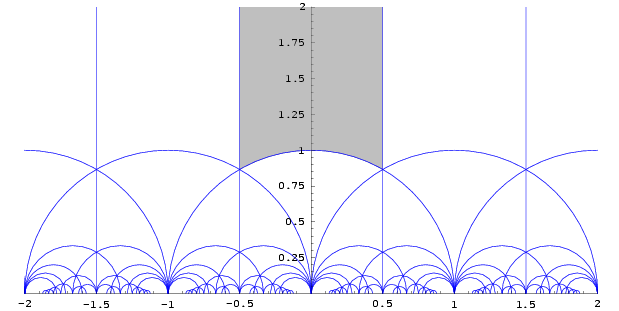
\includegraphics[scale=0.4]{figures/fundamental-domain.png}
    \caption{A fundamental domain (shaded) of the $\PSL_2(\bbZ)$-action on the upper half-plane $\bbC^+$ by \glspl{flt}, and the tiling formed by its orbit.\label{fig fund domain}}
\end{figure}



\begin{defn}\index{Automorphism!Local infinitesimal}
    A \emph{local infinitesimal automorphism} of a Cartan geometry $(P\to M,\eta)$ is an infinitesimal automorphism of the restriction $(\restr{P}{U},\restr{\eta}{U})$ to an open subset $U\subset M$.
\end{defn}

The following lemma establishes a simpler criterion for being a local automorphism.

\begin{lem}[Microlocal is local {{\cite[Lem.~15.6]{McKayCartan}}}]\index{Automorphism!Microlocal infinitesimal}
    Let $(P\overset{\pi}{\to} M,\eta)$ be a Cartan geometry of type $(G,H)$. Let $\varphi:V\to W$ be a (set-theoretic) bijection of open sets $V,W\subset P$ which commutes with the flows of constant vector fields where defined. In addition, assume that for any $m\in \pi(V)$ and connected components $V_0,V_1$ of $P_m\cap V$ there are $p\in V_0$ and $h\in H$ such that $\varphi(p\cdot h)=\varphi(p)\cdot h$ (such a $\varphi$ is called a ``microlocal automorphism''). Then $\varphi$ extends to a unique local automorphism on $\pi^{-1}(\pi(V))$. 

    Similarly, if $X\in\fX(V)$ is a vector field whose flow commutes with the flows of constant vector fields where defined and such that, as above, $X(p\cdot h)=\Phi_{h\ast p}\cdot X(p)$ (a ``microlocal infinitesimal automorphism''), it extends uniquely to a local infinitesimal automorphism on $\pi^{-1}(\pi(V))$. 
\end{lem}
\begin{proof}
    By definition, a microlocal automorphism commutes with the flows up the fibers $P_m$, $m\in M$, of $P$, which are $H$-torsors, so is locally a left translation from one fiber to the other in any principal bundle chart. Hence, it extends globally to such a translation iff we can get it to agree from one component of $V\cap P_m$ to the other on which element it translates by. Hence, it extends to be $H$-invariant. Similarly for the microlocal infinitesimal automorphism.
\end{proof}

\begin{cor}
    If the automorphisms of a Cartan geometry $(P\to M,\eta)$ permute the components of $M$ and the (local) inifinitesimal automorphisms span the tangent space of some point (a dense set of points) of $P$, then the curvature function is constant and its value is an $H$-invariant element of $\frakg\otimes \bigwedge\nolimits^2(\frakg\slash\frakh)^\ast$.
\end{cor}
\begin{proof}
    The preceding lemma allows us to work locally at a point. Since the curvature function must have zero Lie derivative w.r.t.\ any infinitesimal automorphism, if they span the whole tangent space, then the function must be constant. Since it is always $H$-equivariant, its constant value must then be $H$-invariant.
\end{proof}

In particular, if the geometry is torsion-free and complete, then this leads to a Cartan space form. In other words, Cartan space forms are exactly those torsion-free complete Cartan geometries whose infinitesimal automorphisms span the tangent bundle.

\begin{example}
    \begin{enumerate}
        \item For a conformal structure, i.e., one modeled on the conformal sphere $\bbS^n$ with $G=\bbP \Or_{n+1,1}$, it is not difficult to check that $\left(\frakg\otimes \bigwedge\nolimits^2(\frakg\slash\frakh)^\ast\right)^H=0$, so if $\dim \aut=\dim G$, the geometry must be flat.
        \item For a Riemannian geometry, $(G,H)=(\rmE_n,\Or_n)$, and it is easy to check that the space 
        \[\left(\frakg\otimes \bigwedge\nolimits^2(\frakg\slash\frakh)^\ast\right)^H\cong \Hom_{\Or_n}(\bbR^n\times\bbR^n,\frakg)\] 
        is $1$-dimensional, spanned by $(\bf{x},\bf{y})\mapsto \bf{x}\wedge\bf{y}\in\frako_n<\frakg$ (this element generates the rotations in the plane spanned by $\bf{x}$ and $\bf{y}$), cf.\ Example~\ref{ex 1.4.6 Cap}. Hence, if $\dim \aut=\dim G$, then there is a local isometry with either the Euclidean space, the round sphere, or the hyperbolic space.
    \end{enumerate}
\end{example}

\begin{xca}
    Find the infinitesimal automorphisms of the conformal geometry on $\bbS^n$ and on $\RP^n$ for $n\geq 3$.
\end{xca}


While Theorem~\ref{thm 1.5.11 Cap} states that an infinitesimal automorphism is uniquely determined by its value at a single point, there is no guarantee that a given microlocal infinitesimal automorphism can be extended to become global. Each infinitesimal automorphism projects to $M$ to give a vector field that has zeroes arizing from points of $P$ where it is vertical. Outside of such points, there is a dense $H$-invariant open subset of $P$ on which the linear projection of the subspace spanned by $\aut(P,\eta)_p$ achieves maximal rank. Quotienting by $H$, there is a dense open subset of $M$ over which the integral manifolds of $\aut(P,\eta)$ form a foliation. In fact, without going into too much detail, these integral manifolds are smooth even away from that subset. Thus, the leaves of this foliation are covering spaces $\wh{M}\to M$. If these covering spaces are multi-sheeted, we say that the infinitesimal automorphisms are \emph{multivalued}.\index{Automorphism!Multivalued infinitesimal} The group of deck transformations of the covering space is called the \emph{holonomy group of infinitesimal automorphisms}.\index{Holonomy!of infinitesimal automorphisms}

\begin{thm}[Amores II (1980) {{\cite[Thm.~15.8]{McKayCartan}}}]
    Let $(P\to M,\eta)$ be a real analytic Cartan geometry on a connected manifold $M$. Let $X\in \fX(V)$ be a microlocal infinitesimal automorphism defined on a connected open set $V\subset P$. If $M$ is simply connected, then $X$ extends uniquely to an infinitesimal automorphism over $M$. If $M$ is not simply connected, $X$ extends over the universal covering space of $M$, and it descends to an infinitesimal automorphism over $M$ iff $X$ is invariant under the holonomy of infinitesimal automorphisms.
\end{thm}
\begin{proof}
    We can suppose that $M$ is simply connected. Moving by flows of constant vector fields and by the principal $H$-action, we cover $P$ in open sets on each of which we have defined a vector field. Analyticity ensures that, since $X$ is invariant under all constant vector fields initially, and this is an analytic differential equation, this remains true as we extend the domain of $X$. Microlocality is similarly preserved by analyticity and permutation of the constant vector fields under the $H$-action. Hence, each vector field extends uniquely to a local infinitesimal automorphism. At each step in the process, by invariance under the flows, these local infinitesimal automorphisms agree on overlaps. Our vector field $X$ remains $H$-equivariant as we extend it, again by analyticity, so is a section of $\T P\slash H\to M$, a vector bundle over a simply connected manifold, so it does not become multivalued.
\end{proof}

Recall that the soldering form of a Cartan connection $\eta$ is $\theta=\eta+\frakh$. Let us denote it by $\underline{\eta}$ instead, and similarly we use this notation for the quotient of any $\frakg$-valued map by $\frakh$. By Cartan's magic formula, it is easy to see that for a smooth function $f:P\to \frakg$, the associated vector field $X=\eta^{-1}\circ f\in \fX(P)$ preserves the Cartan connection (in particular, is $\frakh$-invariant in the sense that it commutes with $\eta^{-1}(\frakh)$) iff 
\[\dd f+[\eta,f]=\scrK\circ \underline{f}\wedge\underline{\eta}.\]
(The right hand side is nothing but $i_X \Omega^\eta$.) Furthermore, $X$ is an infinitesimal automorphism iff $f$ in addition satisfies $\Phi_h^\ast f=\Ad_h^{-1}f$ for at least one $h$ in each path component of $H$, where $\Phi$ is the principal $H$-action.

This tells us once again that $X$ is determined by its value at a point since we have a total differential equation for $f$. Any $H$-equivariant vector field $X$ on $P$ descends to a vector field $\underline{X}=\pi_\ast X$ on $M$. Just as $X$ is associated to $f$ by $f=\eta(X)$, $\underline{X}$ is associated to $\underline{f}$.

Take two infinitesimal automorphisms $X,Y\in\aut(P,\eta)$ with associated functions $\eta(X),\eta(Y)$. Consider the function $\eta([X,Y])$ corresponding to the bracket $[X,Y]\in \aut(P,\eta)$. The general formula \eqref{eq prop 4.1.6} for the exterior derivative expands to 
\[\eta([X,Y])=[\eta(X),\eta(Y)]-\scrK(\underline{\eta}(X),\underline{\eta}(Y))+\Lie_X (\eta(Y))-\Lie_{Y}(\eta(X)),\]
\index{Curvature-deformed bracket} so the Lie bracket of $\aut(P,\eta)$ is given exactly by the \emph{curvature-deformed bracket} from \eqref{eq deformed bracket}, with the extra terms appearing since $A=\eta(X),B=\eta(Y)$ are no longer constant. From this, the underlying vector field on $M$ is represented by the function
\[\underline{\eta}([X,Y])=\underline{[\eta(X),\eta(Y)]}-\underline{\scrK}(\underline{\eta}(X),\underline{\eta}(Y))+\Lie_X (\underline{\eta}(Y))-\Lie_Y (\underline{\eta}(X)).\]

\begin{prop}[{{\cite[Prop.~15.9]{McKayCartan}}}]
    For a flat Cartan geometry $(P\to M,\eta)$ of type $(G,H)$ on a connected manifold $M$, the Lie algebra $\aut(P,\eta)$ is identified by the developing map with the holonomy-invariant Lie subalgebra of $\frakg$.
\end{prop}
\begin{proof}
    Lift the infinitesimal automorphism to the geometry over the universal cover $\wt M\overset{\wt\pi}{\to}M$, whose bundle is $\wt{P}=\wt{\pi}^\ast P$. Locally, this is identified by the developing map $\dev:\wt{M}\to G\slash H$ with an infinitesimal automorphism of the model geometry, i.e., some element of $\frakg$. Once we match our infinitesimal automorphism with some element of $\frakg$ near some point of $\wt P$, we continue to match in open sets by flowing along constant vector fields. These open sets eventually cover the entire connected component of that point. By $H$-invariance we can extend to all components. So the infinitesimal automorphisms form a Lie subalgebra of $\frakg$ that is invariant under the action of the fundamental group $\pi_1(M)$. The converse is clear.
\end{proof}

\begin{example}
    The conformal geometry of a flat torus $\bbE^n\slash \bbZ^n$ of dimension $\geq 3$ has developing map identifying Euclidean space with a punctured sphere. Infinitesimal automorphisms are vector fields on the sphere vanishing at the puncture and invariant under deck transformations that is, the \emph{cocompact group action} (i.e., the orbit space is compact)\index{Cocompact group action} of the fundamental group of the torus. But the model is algebraic, so these vector fields are invariant under the Zariski closure of the cocompact group action, i.e., under the translations of Euclidean space, hence are themselves translations. The torus has conformal group precisely the torus acting on itself by translation. 
\end{example}

Finally, let us discuss the circumstances under which infinitesimal automorphisms can be recovered from their action on the base manifold. Recall that the kernel $K$ of a Klein geometry $(G,H)$ is the largest normal subgroup of $G$ contained in $H$. Its Lie algebra $\frakk$ is the largest ideal of $\frakg$ contained in $\frakh$, trivial iff $(G,H)$ is locally effective (i.e., $K$ is discrete).

\begin{prop}[Sharpe {{\cite{Sharpe}}}]
    Every infinitesimal automorphism of a Cartan geometry with locally effective model is determined by its projection to the base.
\end{prop}
\begin{proof}
    If $X,Y\in\aut(P,\eta)$ have the same projection, then $Z\coloneqq X-Y\in\aut(P,\eta)$ is tangent to the fibers of $P$. Let $A\coloneqq \eta(Z)$; tangency to the fibers is precisely the statement that $A\in \frakh$, so $\underline{A}=\underline{\eta}(X)=0$. Since $Z$ is an infinitesimal automorphism, we have 
    \[\dd A+[\eta,A]=\scrK\circ \underline{A}\wedge \underline{\eta}=0.\]
    But $A$ is valued in $\frakh$, so $\dd A$ is $\frakh$-valued, while $\eta$ is onto $\frakg$. Hence, $[A,\frakg]\subset \frakh$, so $A$ is valued in the subalgebra of $\frakh$ satisfying this equation. The argument of the last two sentences can be iterated, eventually forcing $A$ to be valued in the largest ideal of $\frakg$ contained in $\frakh$. For a locally effective model, this is zero, so $Z=0$.
\end{proof}






\section{Action of the automorphism group}

Automorphisms commute with the flows of constant vector fields and with the principal action of the structure group. These flows need not be complete, but if defined for some time at some point, they are defined for the same time throughout the orbit of the automorphism group (\emph{automorphism orbit} for short) through that point. Hence, the orbits of the automorphism group are taken to one another by these flows, and by the structure group. Over a connected manifold, this action on the set of orbits is thereby transitive.

\begin{thm}[Kobayashi (1957) {{\cite[Thm.~15.18]{McKayCartan}}}]
    The automorphism orbits of any Cartan geometry $(P\to M,\eta)$ are closed.
\end{thm}
\begin{proof}
    Take a point $p\in P$ in the closure of an automorphism orbit, say $p=\lim_{i\to\infty} g_i(p_0)$ for some $p_0\in P$ and $g_i\in \Aut(P,\eta)$. Define a map $\varphi$ on some neighborhood of $p_0$ by demanding that $\varphi(p_0)=p$ and that $\varphi$ commute with the constant vector fields, i.e., 
    \[\varphi\left(\Fl_t^{\eta^{-1}(A)}(p_0)\right)=\Fl_t^{\eta^{-1}(A)}(p),\quad A\in\frakg;\]
    this uniquely determines $\varphi$ near $p_0$, but we still have to see why it is a local automorphism. Commuting with constant vector fields, convergence of $g_i(p_0)\to p$ in $P$ implies the uniform convergence of $g_i$ with all derivatives as maps $P\to P$. Thus, $\varphi=\lim_i g_i$ near $p_0$. Repeating the construction, $\varphi$ extends smoothly to all of $P$. By the same construction, define a limit for $g_i^{-1}$, thus $\varphi$ is a diffeomorphism and an automorphism, so $p$ lies in the orbit of $p_0$.
\end{proof}


Since we do not yet know that the automorphism orbits are smooth, we define a provisional concept of tangent spaces of subsets of $P$.

\begin{defn}
    Let $(P\to M,\eta)$ be a Cartan geometry. For a subset $S\subset P$, a \emph{tangent vector} at a point $p_0\in S$ is a vector $X\in \T_{p_0}P$ such that, for some sequences $\lambda_i\to\infty$ in $\bbR$ and $A_i\to 0$ in $\frakg$, 
    \[\Fl^{\eta^{-1}(A_i)}_1(p_0)\in S \quad\text{and}\quad \lambda_iA_i\underset{i\to\infty}{\to} \eta(X).\]
    The \emph{tangent space} $\T_{p_0}S$ is the set of tangent vectors to $S$ at $p_0$. This need not be a vector space.
\end{defn}

The tangent spaces of each automorphism orbit are taken to one another by the automorphism group. Automorphisms preserve every constant vector field, so the tangent spaces to each automorphism orbit $\scrO$ consist of the values of the same constant vector fields at all points of $\scrO$. 

In the following, we assume a fixed Cartan geometry $(P\to M,\eta)$ of type $(G,H)$ and do not specify it every time. To each $A\in\frakg$ we also assign the flow of its constant vector field at time $1$:
\[F^A\coloneqq \Fl^{\eta^{-1}(A)}_1\quad\text{for}\quad  A\in\frakg.\]

\begin{lem}[{{\cite[Lem.~15.19]{McKayCartan}}}]\label{lem 12.19 McKay}
    Let $X_i\in \T_{p_0}P$ be a sequence of vectors with $X_i\to 0$ and let $A_i\coloneqq \eta(X_i)\in\frakg$. Suppose that infinitely many among $F^{A_i}(p_0)$ are in the automorphism orbit $\scrO$ of a point $p_0\in P$. After perhaps replacing $(X_i)$ by a subsequence, the lines spanned by the vectors $X_i$ converge to a line tangent to $\scrO$. A constant vector field is somewhere tangent to an orbit iff it is everywhere tangent to that orbit, which occurs iff its flow preserves that orbit.
\end{lem}
\begin{proof}
    Suppose that $F^{A_i}(p_0)=g_i(p_0)$ for some $A_i\to 0$ and $g_i\in \Aut(P,\eta)$. Pick $\lambda_i>0$ such that $\lambda_i A_i$ stays bounded and stays outside of some neighborhood of the origin in $\frakg$. Choosing a subsequence, we can arrange that $\lambda_i A_i$ converges, say $\lambda_i A_i\to A\in\frakg$. Pick a $t\in \bbR$ and let $n_i\coloneqq \lfloor t\lambda_i\rfloor\in\bbN$. But $A_i\to 0$, so $t\lambda_i A_i-n_i A_i\to 0$, i.e., $n_i A_i\to tA$. But $F^{n_iA_i}(p_0)=g_i^{n_i}(p_0)\in\scrO$ while $F^{n_iA_i}(p_0)\to F^{tA}(p_0)$. Since the orbit is closed as a subset of $P$, $F^{tA}(p_0)\in\scrO$ for all $t$. In particular, if $A=\eta(X)$ for a vector $X$ tangent to $\scrO$, then the flow of $A$ preserves $\scrO$.
\end{proof}

\begin{lem}[{{\cite[Lem.~15.20]{McKayCartan}}}]
    The tangent spaces of each automorphism orbit $\scrO\subset P$ are closed cones, i.e., closed subsets of the tangent spaces of $P$ invariant under rescalings by real numbers (including zero and negatives).
\end{lem}
\begin{proof}
    Pick a convergent sequence $X_i\in \T_{p_0}\scrO$. Take sequences $\frakg\ni A_{ij}\underset{j\to 0}{\to} 0$ and sequences $\bbR\ni\lambda_{ij}\underset{j\to 0}{\to} 0$ such that $F^{A_{ij}}(p_0)\in\scrO$ and $\lambda_{ij}A_{ij}\underset{j\to 0}{\to} \eta(X_i)$. Let $A_i\coloneqq A_{ii}$, $\lambda_i\coloneqq \lambda_{ii}$ and apply Lemma~\ref{lem 12.19 McKay}.
\end{proof}

Differentiating the flows of constant vector fields, 
\[F^{tB}\circ F^{tA}=F^{t(A+B)}+\calO(t^2)\]
for any $A,B\in\frakg$ close enough to zero (how close to zero may need to vary with the point of $P$). Recall the curvature-deformed bracket \eqref{eq deformed bracket},
\[[A,B]_p'=[A,B]-\scrK_p(A,B),\quad A,B\in\frakg,\]
defined by the value of the curvature at each point $p\in P$. Taking brackets by commutators of flows,
\begin{align}
    F^{-tB}\circ F^{-sA}\circ F^{tB}\circ F^{sA}&=\Fl^{st[\eta^{-1}(A),\eta^{-1}(B)]}_1+\calO(s,t)^3=\notag\\
    &= \Fl_1^{st\eta^{-1}([A,B]-\scrK(A,B))}+\calO(s,t)^3=\notag\\
    &=F^{st[A,B]'}+\calO(s,t)^3
\end{align}
for any $A,B\in\frakg$ close enough to zero. (Continuing in the same vein, Melnick discovered a \gls{bch}-type formula \cite{Melnick}.)

The next lemma shows that the tangent spaces are actually vector spaces and explains the appearance of the curvature-deformed bracket in our earlier study of Cartan space forms, where the automorphism groups acted transitively on $P$, so $\T \scrO=\T P$.


\begin{lem}[{{\cite[Lem.~15.21]{McKayCartan}}}]
    The tangent spaces of each automorphism orbit in $P$ are linear subspaces of the tangent spaces of $P$, and Lie algebras under the curvature-deformed bracket.
\end{lem}
\begin{proof}
    Take tangent vectors $X,X'\in\T_{p_0}\scrO$. Let $A\coloneqq \eta(X)$, $A'\coloneqq \eta(X')$, so there are sequences $\lambda_i,\lambda_i'\underset{i\to\infty}{\to}\infty$ and $A_i,A_i'\to 0$ for which 
    \[F^{A_i}(p_0),F^{A_i'}(p_0)\in\scrO,\]
    say 
    \[g_i(p_0)=F^{A_i}(p_0),\quad g_i'(p_0)=F^{A_i'}(p_0)\]
    for some $g_i,g_i'\in\Aut(P,\eta)$ and $\lambda_iA_i\to A$ and $\lambda_i'A_i'\to A'$.

    Pick any sequence $t_i\to \infty$ of positive numbers. Replacing $\lambda_i,\lambda_i'$ by subsequences, we can assume that both grow faster than $t_i$: $\frac{\lambda_i}{t_i},\frac{\lambda_i'}{t_i}\to \infty$. Let $n_i=\lfloor\frac{\lambda_i}{t_i}\rfloor $ and $n_i'=\lfloor\frac{\lambda_i'}{t_i}\rfloor$, so $\frac{\lambda_i}{n_i},\frac{\lambda_i'}{n_i'}\approx t_i\to \infty$. Take new $A_i$, $A_i'$, $\lambda_i$, $\lambda_i'$ equal to the old $n_iA_i$, $n_i'A_i'$, $\frac{\lambda_i}{n_i}$, $\frac{\lambda_i'}{n_i'}$ so that we can assume that $\lambda_i/\lambda_i'\to 1$. We have 
    \[g_i'\circ g_i(p_0) = g_i'\circ F^{A_i}(p_0)=F^{A_i}\circ g_i'(p_0)=F^{A_i}\circ F^{A_i'}(p_0)=F^{A_i+A_i'+\cdots}(p_0)\]
    and 
    \[\lambda_i(A_i+A_i'+\cdots )=\lambda_i A_i+\frac{\lambda_i}{\lambda_i'}\lambda_i'A_i'+\cdots\to A+A'.\]
    By Lemma~\ref{lem 12.19 McKay}, the lines spanned by $A_i+A_i'$ converge to a tangent line to the orbit, the span of $A+A'$. By the same argument, using the bracket by commutators of flows, $[A,B]'_p$ is also in the tangent space, so it's a Lie algebra.
\end{proof}

Now that we know that the tangent spaces have the same dimension, we can use them to construct slices for the action of the automorphism group, which will imply that the orbits are smooth. Let $p_0\in P$ and let $\scrO$ be its automorphism orbit. As usual, a \emph{slice} at $p_0$ is a smooth embedding $\varphi:U\to P$ of an open $0$-neighborhood $U\subset V$ in a finite-dimensional vector space $V$ such that $\varphi(0)=p_0$, $\varphi^{-1}(\scrO)=\{0\}$, and the image is transversal to the orbit at $p_0$: 
\[\varphi_{\ast 0}(V)\oplus\T_{p_0}\scrO=\T_p P.\]

\begin{lem}[{{\cite[Lem.~15.22]{McKayCartan}}}]\label{lem 12.22 McKay}
    Let $V<\T_{p_0}P$ be a subspace complementary to $\T_{p_0}\scrO$. Then there is an open $0$-neighborhood $U\subset V$ such that the following map is a slice:
    \[\varphi:U\to P,\quad  v\mapsto F^{\eta(v)}(p_0).\]
\end{lem}
\begin{proof}
    Let $V'\coloneqq \eta(V)<\frakg$, which is a subspace complementary to $T'\coloneqq \eta(\T_{p_0}\scrO)$. If there is a sequence of elements $A_i\to 0$ with $A_i\in V'$ and with $F^{A_i}(p_0)\in \scrO$, then as above we can find a convergent subsequence such that the lines spanned by $A_i$ converge in $\T_{p_0}P$ to some line spanned by some $A\neq 0$. Since $V'<\frakg$ is a subspace, it is a closed subset, so $A_i\in V'$ implies $A\in V'$. By definition of tangent spaces, $A\in T'$, so $A\in T'$. Since $T'\cap V'=\{0\}$, we conclude $A=0$, a contradiction. Thus, there is no such sequence, i.e., there is an open $0$-neighborhood $U'\subset V'$ in which no point $A$ has $F^A(p_0)\in \scrO$. Take the associated set $U=\eta^{-1}_{p_0}(U')\subset V$. By shrinking $U$, we can arrange that $A\mapsto F^A(p_0)$ is defined on $U$ and is an embedding.
\end{proof}

The following lemma constructs slice charts for the orbit, turning it into an embedded submanifold.

\begin{lem}[{{\cite[Lem.~15.23]{McKayCartan}}}]\label{lem 12.23 McKay}
    Let $V<\T_{p_0}\scrO$ be a subspace complementary to $\T_{p_0}\scrO$. Pick $0$-neighborhoods $U\subset V$ and $W\subset \T_{p_0}\scrO$. If the open sets are small enough then the map 
    \[\varphi:V\times W\to P,\quad (v,w)\mapsto F^{\eta(v)}\circ F^{\eta(w)}(p_0)\]
    is a diffeomorphism to an open subset of $P$ an a slice for any fixed $w$.
\end{lem}
\begin{proof}
    By the \gls{inmt}, we can pick small enough open sets $U,W$ to ensure that $\varphi$ is a diffeomorphism to its image, an open set $U_P\subset P$. For any $w$, $\varphi(0,w)\in\scrO$ by Lemma~\ref{lem 12.19 McKay}. We can pick $U$ small enough to ensure that $v\mapsto \varphi(v,0)$ is a slice by Lemma~\ref{lem 12.22 McKay}, so stays outside $\scrO$ except at $v=0$. Let $U'\coloneqq \eta_{p_0}(U)\subset \frakg$ and $W'\coloneqq \eta_p(W)\subset \frakg$. If $\varphi(v,w)\in\scrO$ then we have 
    \[F^{\eta(v)}\circ F^{\eta(w)}(p_0)=g(p_0),\]
    for some automorphism $g\in\Aut(P,\eta)$. Thus, $F^{-\eta(v)}(p_0)=g^{-1}(\circ ^{\eta(w)}(p_0)$ lies in $\scrO$, and $\eta_p(v)=0$, so $v=0$.
\end{proof}

\begin{cor}
    Every automorphism orbit of a Cartan geometry is a closed embedded submanifold.
\end{cor}

\begin{cor}[{{\cite[Cor.~15.25]{McKayCartan}}}]
    Let $M$ be connected, and pick an automorphism orbit $\scrO$ through a point $p_0\in P$. The orbit is a closed embedded submanifold, and the action of automorphisms is free, so we can endow the group $\Aut(P,\eta)$ with the smooth structue diffeomorphic to that of $\scrO$ via the map $g\mapsto g(p_0)$. Then 
    \begin{enumerate}
        \item this smooth structure turns the group $\Aut(P,\eta)$ into a Lie group;
        \item upon changing the point of $p_0$, the Lie group structure undergoes an isomorphism given by the flows of constant vector fields and the principal action of the structure group;
        \item $\Aut(P,\eta)$ acts smoothly on $P$ and $M$.
    \end{enumerate}
\end{cor}
\begin{proof}
    Take $g,h\in\Aut(P,\eta)$. We want to prove that $gh$ is a smooth function of $g,h$, i.e., that $g\circ h(p_0)$ is a smooth function of $g(p_0)$ and $h(p_0)$. We need only vary $g,h$ by flows $F^A$, $F^B$, since these flows provide local coordinates $A,B\in V<\frakg$ on the orbit near each point. Thus, we need to prove that $F^A\circ g\circ F^B\circ h(p_0)$
    depends smoothly on $A$ and $B$, which is obvious. The same expression demonstrates the smoothness of the action.
\end{proof}

Finally, now that we have a free Lie group action of $\Aut(P,\eta)$ on $P$, we can ask whether this action is proper, so that $P$ can be treated as a principal $\Aut(P,\eta)$-bundle. Recall that an action $(g,m)\mapsto g\cdot m$ is called proper when the map $(g,m)\mapsto (g\cdot m,m)$ is proper. 

\begin{cor}[{{\cite[Cor.~15.26]{McKayCartan}}}]
    If $M$ is connected, then the Lie group action of $\Aut(P,\eta)$ on $P$ is free and proper.
\end{cor}
\begin{proof}
    By Corollary~\ref{cor 6.3.3 RS1}(2), the action is proper iff for any sequences $g_i\in \Aut(P,\eta)$ and $p_i\in P$, if both $(g_i(p_i))$ and $(p_i)$ converge in $P$, then some subsequence $(g_{i_j})$ converges in the group.

    The topology of $\Aut(P,\eta)$ is that of the orbit through any one point $p$, so $g_i(p)\to g(p)$ iff $g_i\to g$. After taking a subsequence $p_i\coloneqq F^{A_i}\circ F^{B_i}(p)$ for some $A_i,B_i\to 0$ as in Lemma~\ref{lem 12.23 McKay}. Similarly, after taking another subsequence, we can write $g_i(p_i)=F^{C_i}\circ F^{D_i}(q)$ for some $C_i,D_i\to 0$ and $q\in P$. Combining these two formulas, we see that
    \[g_i(p)=F^{-B_i}\circ F^{-A_i}\circ F^{C_i}\circ F^{D_i}(q)\]
    approaches $q$ by continuity of the flows of the constant vector fields. Since orbits are closed, $q=g(p)$ for some $g\in \Aut(P,\eta)$, so $g_i(p)\to g(p)$ and thus $g_i\to g$, as required.
\end{proof}

By Corollary~\ref{cor 6.5.1 RS1}, the quotient by a free and proper Lie group action is a smooth manifold, and the quotient map is a \gls{pfb}. The action of automorphisms is a left action, so this will be a left quotient. We summarize our results on automorphisms in the following main theorem.

\begin{thm}[{{\cite[Thm.~15.13]{McKayCartan}}}]\label{thm 12.13 McKay}
    If $(P\to M,\eta)$ is a Cartan geometry of type $(G,H)$ on a connected manifold $M$. Then:
    \begin{enumerate}
        \item The automorphism group $\Aut(P,\eta)$ admits a unique Lie group structure (up to isomorphism) for which the quotient map $P\to \Aut(P,\eta)\bslash P$ is a smooth principal bundle;
        \item The Lie algebra of $\Aut(P,\eta)$ is the set of complete infinitesimal automorphisms. 
        \item The constant vector fields descend to smooth vector fields on $\Aut(P,\eta)\bslash P$ spanning every tangent space.
        \item The principal $H$-action descends to a smooth $H$-action on $\Aut(P,\eta)\bslash P$.
    \end{enumerate} 
\end{thm}
\begin{proof}
    Only items 2-4 are yet unproven. Complete infinitesimal automorphisms generate automorphic flows lying in the identity component of $\Aut(P,\eta)$. By the Analytic Subgroup Theorem~\ref{thm analytic subgroup}, they belong to the Lie algebra of $\Aut(P,\eta)$. Conversely, consider an automorphism orbit with basepoint $p_0$ as a copy of the Lie group $\Aut(P,\eta)$ and consider a right-invariant vector field on it. The flows of constant vector fields and the action of the structure group push this vector field all around $P$ to produce a global infinitesimal automorphism. It is complete because it is a right-invariant vector field for the Lie group structure of each automorphism orbit.

    3 is obvious since constant vector fields are $\Aut(P,\eta)$-invariant. 4 follows from the fact that $H$ acts by bundle morphisms on the bundle $P\to \Aut(P,\eta)\bslash P$. 
\end{proof}

Sometimes a generalization of this result to disconnected base manifolds is useful. This is shown in the following exercise and theorem.

\begin{xca}
    Let $(P\to M,\eta)$ be a Cartan geometry over a connected $M$. Prove that the topology of the automorphism group determined by identifying it with an orbit in $P$ is the topology of pointwise convergece, but is also the compact-open topology on it as a collection of maps of $P$, and is also the topology of uniform convergence on compact sets with all derivatives.
\end{xca}

\begin{thm}[{{\cite[Thm.~15.28]{McKayCartan}}}]\label{lem thm 12.28 McKay}
    Suppose $\varGamma$ is a group consisting of some automorphisms of a Cartan geometry $(P\to M,\eta)$, closed in the topology of uniform convergence on compact sets with all derivatives. Suppose that, for every connected component $M'\subset M$, the only element of $\varGamma$ that fixes every point of $P$ above $M'$ is the identity. Then $\varGamma$ is a Lie group acting smoothly on $P$ and $M$ and the quotient map $P\to \varGamma\bslash P$ is a principal $\varGamma$-bundle. There is a finite set of smooth $\varGamma$-invariant functions on $P$ that distinguish $\varGamma$-orbits.
\end{thm}
\begin{proof}
    Suppose that $\varGamma$ fixes a point of $P$. Commuting with the $H$-action and constant vector fields, $\varGamma$ fixes every element of $P$ above some component $M'\subset M$, so is the identity. Hence, $\varGamma$ acts freely. The rest of the proof is identical to the original proof of the properness of the action of automorphism groups. The topology of $\varGamma$ is almost irrelevant by the preceding exercise. As the quotient $\varGamma\bslash P$ is a manifold, it admits an embedding into some $\bbR^s$ by the Whitney Embedding Theorem~\ref{thm whitney embedding}. Take the coordinate functions of such an embedding as out finite set of smooth functions.
\end{proof}

All automorphisms that fix a point in the base are vertical automorphisms given by some principal right actions (note that generic principal actions are usually not automorphisms, even in Klein geometries):

\begin{lem}[{{\cite[Lem.~15.27]{McKayCartan}}}]
    Let $(P\to M,\eta)$ be a Cartan geometry. For a point $m\in M$, its stabilizer $\Aut(P,\eta)_m$ is a closed subgroup of $\Aut(P,\eta)$ contained inside $H\cap \Aut(P,\eta)$, where by $H$ we mean the set of principal right $H$-actions.
\end{lem}
\begin{proof}
    We can assume that $M$ is connected, \gls{wlog}. Let $G'\coloneqq \Aut(P,\eta)$ and $H'\coloneqq \Aut(P,\eta)_m$. Pick a point $p\in P_m$. Embed $G'\to P$ by the orbit map $g\mapsto g(p)$. Each $k\in H'$ moves $p$ to a point of the same fiber, which is an $H$-torsor, so $k(p)=p\cdot \wb{k}$ for some $\wb k\in H$. But since $H'(p)=G'(p)\cap (p\cdot H)$, the image of $\phi:k\mapsto \wb{k}$ is a closed embedded submanifold. $\phi$ is also injective because the $H$-action is free, and clearly an anti-homomorphism, so its image is a closed subgroup.
\end{proof}

In particular, if $H$ is compact, the stabilizers of all points of $M$ are also compact. By applying Corollary~\ref{cor 6.3.3 RS1}(3), we get the following important result.

\begin{cor}
    If $M$ is compact, then any Cartan geometry with a compact structure group $H$ has a compact automorphism group.
\end{cor}

\begin{cor}\label{cor compact isometry group}\index{Isometry group}
    The isometry group of any compact Riemannian manifold is a compact Lie group.
\end{cor}

\begin{xca}
    Suppose that the model is $(G,H)$ and $\Aut(P,\eta)$ acts transitively on $P$, so $P$ is a torsor for this group. Let $\fraka$ be the Lie algebra of $\Aut(P,\eta)$. Prove that the Cartan connection has the form $\varLambda\circ\theta_{\Aut}$ for some constant linear map $\varLambda\in\frakg\otimes\fraka^\ast$, where $\theta_{\Aut}$ is the Maurer-Cartan form of $\Aut(P,\eta)\cong P$.
\end{xca}


\begin{cor}[{{\cite[Cor.~15.29]{McKayCartan}}}]
    Let $(P\to M,\eta)$ be a Cartan geometry on a connected manifold $M$. Then, along each automorphism orbit $\scrO$, the constant vector fields which are tangent to $\scrO$ are exactly the left-invariant vector fields of $\scrO$ as a $\Aut(P,\eta)$-torsor. In particular, the Lie bracket of the Lie algebra of $\Aut(P,\eta)$ is identified, via $\eta$, with the curvature-deformed bracket on $\frakg$.
\end{cor}
\begin{proof}
    Automorphisms take tangent vectors of $\scrO$ to tangent vectors of $\scrO$ and constant vector fields to constant vector fields. Hence, the constant vector fields tangent to $\scrO$ at a point are everywhere tangent to $\scrO$, and hence are the left-invariant vector fields. By dimension counting, this covers all left-invariant vector fields. Their bracket is the curvature-deformed bracket, as we saw above.
\end{proof}


\PRLsep


In the remainder of this \sect, we discuss \emph{automorphisms of submanifolds}.


\begin{defn}
    Let $(P\to M,\eta)$ be a Cartan geometry of type $(G,H)$ and let $i:S\hookrightarrow M$ be an immersed submanifold of $M$. An \emph{automorphism of $S$} is an automorphism of the Cartan geometry whose base map commutes with $i$ (i.e., takes $S$ to itself). The group of all automorphisms of $S$ is denoted by $\Aut_S(P,\eta)$ and is by definition a subgroup of $\Aut(P,\eta)=\Aut_M(P,\eta)$.
\end{defn}


\begin{example}
    \begin{enumerate}
        \item An automorphism of an immersed surface $\varSigma\hookrightarrow\bbE^3$ is a diffeomorphism of $\varSigma$ and a rigid motion of Euclidean space which matches the diffeomorphism along $\varSigma$.
        \item If $S$ is a closed embedded submanifold of $M$, then its automorphisms form a closed subgroup of $\Aut(P,\eta)$, cf.\ \cite[p.~44]{Mimura}.
        \item  Consider an immersed surface $\varSigma$ consisting of several disjoint connected components mapped to the same surface in $\bbE^3$. The automorphism group is not a subgroup of the rigid motions. Pick a dense subset of each component surface so that the two subsets are carried by the diffeomorphism to disjoint sets in $\bbE^3$; our immersion is injective on the union of those subsets, a dense subset of $\varSigma$. If we take a countable collection of connected surfaces, we find an automorphism group with uncountably many components.
        \item Now suppose that the immersed surface $\varSigma$ consists of all planes parallel to and at a rational distance from a given plane. The automorphism group acts properly on $\varSigma$ as a Lie group, but does not act properly on $\bbE^3$, even though $\varSigma$ is injectively immersed.
        \item  In the previous example with $\varSigma$ consisting of the same planes, equip $\bbE^3$ with its standard flat conformal geometry. Suppose that the origin belongs to $\varSigma$. Rescalings of $\bbE^3$ by rational numbers act on $\varSigma$ as automorphisms. A sequence of such automorphisms by rational numbers converging to an irrational one acts as automorphisms on the plane through the origin, but has no limit in $\varSigma$ on any of the other planes. Therefore, we want a topology on the automorphism group of $\varSigma$ so that this sequence won't converge; in this example, we want the discrete topology on those rational rescalings.
        \item Consider a dense (irrational slope) line in the flat affine torus, $\bbR\hookrightarrow\bbT^2$, so the model is $(\U_1\times\U_1,\{e\})$. The automorphisms are the translations of $\bbT^2$, acting as a subgroup of $\bbT^2$, hence a Lie group $\bbR$ mapping $\bbR\hookrightarrow \bbT^2$ as an immersed subgroup. 
        \item Take a homogeneous space $M=G\slash H$. Let $M_\delta$ be $M$ with the discrete topology, let $H_\delta$ be the same as $H$, and let $G_\delta$ be $G$ with the topology whose open sets are unions of translates $gU$ of open sets $U\subset H$. The identity map $M_\delta\to M$ is equivariant for the identity map $G_\delta\to G$, so an equivariant immersion with automorphism group $G_\delta$. If $\dim M>0$, this automorphism group is an immersed but not embedded subgroup of $G$.
        \item Consider the map $S=\bbR\to \bbC=M$ given by $x\mapsto \rme^{\i x}$. For each real $c\in \bbR$, the map $x\mapsto x+c$ on $\bbR$ and the rotation of $\bbC$ around the origin by angle $x$ commute, and these are the Euclidean automorphisms of this immersion. So the automorphism group of $S$ is $\bbR$ equipped with a non-injective immersion $\bbR\to \SO_2\ltimes\bbR$.
    \end{enumerate}
\end{example}

Let $P_S\coloneqq i^\ast P$. Then $P_S\to P$ is an immersed subbundle with $\dim P_S=\dim S+\dim H$ and we have a commuting diagram 
\[\begin{tikzcd}
    P_S\arrow[r]\arrow[d] & P\arrow[d]\\
    S \arrow[r] & M.
\end{tikzcd}\]

For the proof of the next theorem, the following enrichment of the notion of a Cartan geometry will be useful. It is a direct analog of the notion of extended coframe from Definition~\ref{def extended coframe} if one thinks of a Cartan connection as a coframe.

\begin{defn}\index{Decorated Cartan geometry}
    A decorated Cartan geometry is a Cartan geometry $(P\to M,\eta)$ equipped with a collection (perhaps infinite) of smooth maps $f_\alpha:P\to M_\alpha$ to some smooth manifolds $M_\alpha$. Each $f_\alpha$ is called a \emph{decoration}.
\end{defn}

\begin{example}
    Any vector field $X\in\fX(M)$ is naturally identified with an $H$-equivariant map $\wt X=\theta(\pi^\ast X):P\to \frakg\slash\frakh$. Thus, any tensor field on $M$ is a decoration. In particular, an action of a finite-dimensional Lie algebra is a decoration.
\end{example}

Clearly, the automorphism group of a decorated Cartan geometry is a closed subgroup of the automorphism group of the undecorated geometry. Thus, all of our results about the action of the automorphism group extend trivially to decorated geometries.

\begin{thm}[{{\cite[Thm.~15.33]{McKayCartan}}}]
    Let $(P\to M,\eta)$ be a Cartan geometry on a connected manifold $M$. Let $(S,i:S\to M)$ be an immersed submanifold such that $i$ is injective on a dense subset of $S$. Then the automorphisms of $S$ form a finite-dimensional Lie group for a unique Lie group structure such that the quotient map 
    \[P_S\to \Aut_S(P,\eta)\bslash P_S\]
    is a smooth principal $\Aut_S(P,\eta)$-bundle. This Lie group acts smoothly on $P_S$, $S$, $P$, and $M$. The Lie group homomorphism $\Aut_S(P,\eta)\to \Aut(P,\eta)$ is an immersion.
\end{thm}
\begin{proof}
    Let $\varGamma$ be the group of diffeomorphisms of $P_S$ preserving $\restr{\eta}{P_S}$ and commuting with the principal $H$-action, with the topology of uniform convergence on compact sets with all derivatives. Then $\Aut_S(P,\eta)$ is a subgroup of $\varGamma\times \Aut(P,\eta)$. Take a linear surjection $\pi:\frakg\to \frakg'$ to a vector space $\frakg'$ of dimension $\dim P_S$. Let $\eta'\coloneqq \pi\circ\eta$. Let $P'\subset P_S$ be the open subset consisting of all points at which $\eta'$ is a linear isomorphism on the tangent spaces. By varying the map $\pi$, we cover $P_S$ is these open sets $P'$. On each $P'$, $\eta'$ is a coframing, so a Cartan connection with trivial infinitesimal model $(\frakg',0)$ and base space $P'$ (not $S$). Since $\eta'$ is a linear isomorphism on each tangent space of $P'$, $\eta=a\circ \eta'$ for a unique smooth map 
    \[a:P_S\to \frakg\otimes(\frakg')^\ast.\]
    Thus, $\eta$ is determined by the decorated Cartan geometry of $P'$ with decoration $a$. Add the composition $P'\hookrightarrow P_S\hookrightarrow P\to P\slash \Aut(P,\eta)$
    as another decoration to $P'$. Inside the automorphism group of this decorated Cartan geometry, $\Aut_S(P,\eta)$ is the closed subgroup commuting with the $H$-action.

    If some autoorphism in $\Aut_S(P,\eta)$ fixes a point of $P_S$, then it fixes the image of that point in $P$, so acts on $P$ trivially, so acts on $M$ trivially. It then fixes every point of the dense open subset of $S$ on whicn $i$ is injective, so it fixes every point of $S$ and of $P$ and hence of $P_S\subset S\times P$. In particular, $\Aut_S(P,\eta)$ acts freely on $P_S$, and thus on $P'$. Apply Theorem~\ref{lem thm 12.28 McKay} to find that $P'\to \Aut_S(P,\eta)\bslash P'$ is a principal bundle, for each of the $\Aut_S(P,\eta)$-invariant open subsets $P'\subset P_S$. If $\Aut_S(P,\eta)\to \Aut(P,\eta)$ maps some vector to zero, it maps some infinitesimal automorphism on $P_S$ to zero in $P$, which contradicts the fact that $P_S\to P$ is an immersion. 
\end{proof}

% \begin{cor}
%     Let $(P\to M,\eta)$ be a Cartan geometry over a manifold $M$ with finitely many connected components. Let $(S,i:S\to M)$ be an immersed submanifold such that $i$ is injective on a dense subset of $S$. Then $\Aut_S(P,\eta)$ is a finite-dimensional Lie group acting smoothly on $P_S$, $P$, $P$, and $M$, and an immersed Lie subgroup of $\Aut(P,\eta)$.
% \end{cor}


\section{Homogeneous Cartan geometries}

We now take a brief look at a class of Cartan geometries that are a generalization of the concept of Cartan space forms. Recall that all Cartan space forms ended up being mutations of complete flat Cartan geometries. This actually has to do with the fact that a complete flat Cartan geometry has only one automorphism orbit, and that orbit lifts to a Lie group. In practice, however, it is more likely that the action is transitive only on the base manifold, and the completeness condition is also overly restrictive.


\begin{defn}[Homogeneous Cartan geometry]\index{Homogeneous Cartan geometry}
    A Cartan geometry $(P\to M,\eta)$ is called homogeneous if its automorphism group acts transitively on $M$.
\end{defn}

The following example shows that homogeneous geometries can indeed be incomplete.

\begin{example}
    The flat torus has a flat Riemannian geometry invariant under translations, hence a homogeneous projective connection. However, this geometry is incomplete by Example~\ref{ex flat projective structures}. Similarly, the conformal geometry of the flat torus of dimension $3$ or more is homogeneous but not complete by Example~\ref{ex flat conformal structures}.
\end{example}

The question for this \sect\ is: \emph{can we find homogeneous Cartan geometries with a given model, and perhaps even classify all such geometries?} Suppose $(P\to M,\eta)$ is a homogeneous Cartan geometry with model $(G,H)$. By Theorem~\ref{thm 12.13 McKay}, the automorphism group embeds into the total space $P$ as an automorphism orbit. Since the Cartan geometry is invariant under automorphisms, the curvature function $\scrK$ is constant along each automorphism orbit $\scrO$. Meanwhile, along the fibers it transforms under the usual representation of $H$ on the curvature module $\bigwedge\nolimits^2(\frakg\slash\frakh)^\ast\otimes\frakg$. 

To classify homogeneous geometries of this type, we can use the structure group $H$ to being the curvature to some normal form, say some fixed value $\scrK_0$. Let $H_1\emb H$ be the stabilizer of $\scrK_0$ and let $P_1\subset P$ be the set on which $\scrK=\scrK_0$. Then $P_1\to M$ is a right principal $H_1$-bundle. Our automorphism orbit $\scrO$ is contained inside $P_1$. On $\scrO$, the structure equation 
\[\dd\eta+\frac12[\eta,\eta]=\frac12\scrK_0\circ \theta\wedge\theta\label{eq 12469}\]
differentiates to expand out into expressions involving only $\dd\eta$ and $\dd\theta$. But $\theta=\eta+\frakh$, so everything expands in terms of $\dd\eta$, which the structure equation turns back into an expression in $\eta$ and $\scrK_0$. This could give additional algebraic compatibility conditions on $\scrK_0$.

There is another source of relations. On $P_1$, the Cartan connection $\eta$ may no longer be a global coframe. Rather, if $H_1\emb H$ has positive codimension, then $\eta+\frakh_1$ is horizontal, say 
\[\eta+\frakh_1=a\circ\theta\]
for some $H_1$-equivariant $a:P_1\to (\frakg\slash\frakh_1)\otimes(\frakg\slash\frakh)^\ast$. Clearly, $a$ is also invariant under the automorphism group, hence constant on our orbit. Repeating the process, pick some constant value $a_0$ for $a$, let $H_2\emb H$ be its stabilizer, and let $P_2\subset P_1$ be the set on which $a=a_0$, so it is a principal $H_2$-bundle. Again, when differentiating the structure equations on $\scrO\subset P_2$, they expand out to equations in the components of $\eta,a_0,\scrK_0$. These equations may force more algebraic relations among $a_0,\scrK_0$.

On $P_2$, we may write 
\[\eta+\frakh_2=b\circ \theta\]
for a unique $H_2$-equivariant $b:P_2\to (\frakg\slash\frakh_2)\otimes(\frakg\slash\frakh)^\ast$, which projects to $a_0$ under the obvious quotient map $\frakg\slash\frakh_2\to\frakg\slash\frakh_1$.

Continue this way until we find that $\dim H_{k+1}=\dim H_k$, so we don't get any new invariants. (In particular, if some $H_j$ is a linear algebraic group, then all subsequent $H_{j+1}$ etc.\ are linear algebraic, each contained in the previous. By the ascending chain condition, the sequence eventually stabilizes, say all equal to some $H_0\emb H$.) Eventually, $\eta+\frakh_0=c_0\circ\theta$ is a constant, and plugging into the structure equations \eqref{eq 12469} yields algebraic equations on $c_0,\scrK_0$ which are satisfied by our initial choice of $c_0,\scrK_0$. These equations then determine structure constants for the remaining linearly independent components $\eta^i$ of $\eta$. By our discussion above, these are the structure equations of a Lie group. Of course, this way we only find a Lie algebra and the embedding of various subalgebras. It remains to determine the actual Lie group of automorphisms of the corresponding homogeneous geometry, assuming it even exists. There is still a possibility that the resulting structure equations are those of a Lie group for which the Lie algebra of $H_0$ does not exponentiate to a closed subgroup. Moreover, it may not be clear how to find a more explicit geometric description of this Lie algebra.







\section{Example: homogeneous affine surfaces}


Consider how we might classify homogeneous surfaces $\varSigma$ modeled on the affine plane $\bbA(\bbR^2)=\Aff_2(\bbR)\slash \GL_2(\bbR)$ with an affine connection invariant under a group of automorphisms acting transitively on the surface. The automorphisms preserve the affine connection, and thus, in particular, preserve the torsion tensor and the torsion-free affine connection obtained by subtracting off the torsion. Hence, we may assume that the connection is torsion-free.

As usual, we write affine transformations as $\left(\begin{smallmatrix}
    g & \bf{x}\\ 0 & 1
\end{smallmatrix}\right)$, so the Cartan connection reads $\eta=\left(\begin{smallmatrix}
    \omega & \theta\\ 0 & 0
\end{smallmatrix}\right)$. The torsion-free condition is exactly $\dd\theta+\omega\wedge\theta=0$, and the curvature is given by 
\[\dd\omega+\omega\wedge\omega=K \theta^1\wedge\theta^2,\label{eq 129521}\]
where $K\in\frakgl_2(\bbR)$ is represented by a $2\times 2$ matrix multiplying the scalar $2$-form $\theta^1\wedge\theta^2$.

\textbf{Flat surfaces.} In the case $K=0$, the affine connection  is flat, so the affine Cartan geometry is flat, thus locally isomorphic to the model. If it is not globally isomorphic to the model, then it develops to the model via the developing map which is a local isomorphism. Assuming $\varSigma$ is connected, each automorphism then extends uniquely to an automorphism of the affine plane. So, $\varSigma$ is a covering space of an open set in the plane, homogeneous under a subgroup of the affine group. 

A homogeneous Cartan geometry $(P\to M,\eta)$ is called \emph{subordinate} to another $(P'\to M',\eta')$, with the same model $(G,H)$, if there is an $H$-equivariant local diffeomorphism $P\to P'$ that is also equivariant under some homomorphism of the automorphism groups. For example, the hyperbolic half-plane $\bbC^+$ has a projective connection induced from its Riemannian geometry, and is equivariantly embedded into the projective plane, hence subordinate to the model projective geometry. 

We would like to find the maximal homogeneous affine surfaces, ordered by subordinacy. We leave it to the reader to classify non-maximal homogeneous affine surfaces subordinate to these. From now on, we can suppose that $K\neq 0$.

\textbf{Normalizing curvature.} Any matrix $K=(K^i_j)$ could, in principle, show up in some homogeneous affine surface. But on any given automorphism orbit $K$ is constant. The automorphism group commutes with the $H$-action, so the $H$-action permutes the automorphism orbits while transforming $K$ in the usual way. Take the structure equations \eqref{eq 129521} and apply the right action $\Phi_h$ by an element $h\in H$, so in matrix notation, $\Phi_h^\ast\omega=h^{-1}\cdot \omega\cdot h$ and $\Phi_h^\ast\theta=h^{-1}\cdot\theta$. We get 
\begin{align}
    0&=h^{-1}(\dd\omega+\omega\wedge\omega)h-(\Phi^\ast_h K)\det h^{-1}\theta^1\wedge\theta^2=\notag\\
    &=(h^{-1} K h-\det h^{-1}\Phi_h^\ast K)\theta^1\wedge\theta^2,
\end{align}
which implies 
\[\Phi_h^\ast K=(\det h)h^{-1} K h.\]
Thus, by choosing the right $h$, we can move to an orbit where $ K$ is in its real Jordan normal form up to a scale factor, constant on the orbit. By picking $h=\lambda\rmI$ for any $\lambda\neq 0$, we can then move to an orbit with value of $ K$ scaled by $\lambda^2$. Thus, we can assume that $\det K\in \{-1,0,1\}$. \textbf{If $ K$ is real diagonalizable}, we can swap the order of the two eigenvalues using $h=\left(\begin{smallmatrix}
    0 & 1\\ -1 & 0
\end{smallmatrix}\right)$, and $h=\left(\begin{smallmatrix}
    1 & 0\\ 0 & -1
\end{smallmatrix}\right)$ can swap the signs of both eigenvalues. Thus, we can assume that the eigenvalues are in order, i.e., either 
\[ K=\begin{pmatrix}
    r & 0 \\ 0 & \pm 1/r
\end{pmatrix},\quad r\geq 1\]
or 
\[ K=\begin{pmatrix}
    1 & 0 \\ 0 & 0
\end{pmatrix},\]
or $ K=0$. \textbf{If $ K$ is not real diagonalizable but complex diagonalizable} (so, two coinciding complex eigenvalues), then $\det K>0$ and so we can assume $\det K=1$, so, viewed as a unit complex number,
\[K=\rme^{\i\alpha},\quad \theta\in (-\pi,\pi)\setminus\{0\}.\]
Finally, \textbf{if $ K$ is not complex diagonalizable}, then it has a generalized eigenspace, so a double eigenvalue, nonnegative determinant, so either $\det K=0$ or $\det K=1$. In terms of the complex Jordan normal form, we have three options:
\[ K=\begin{pmatrix}
    1 & \pm 1\\
    0 & 1
\end{pmatrix} \quad \text{or}\quad \begin{pmatrix}
    0 & 1\\
    0 & 0
\end{pmatrix} \quad \text{or}\quad \begin{pmatrix}
    0 & -1\\
    0 & 0
\end{pmatrix}.\]
Let $H_0\emb H$ be the subgroup preserving the normal form of $ K$, i.e. 
\[H_0\coloneqq \{h\in H\mid (\det h)  K h=h K\}.\]
The set of points $P_0\subset P$ at which $ K$ takes on this normal form is a principal $H_0$-bundle.

If $\det K\neq 0$, so $\det K=\pm 1$, taking a determinant tells us that the elements of $H_0$ have determinant $\pm 1$ and those with determinant $1$ are precisely those that commute with $K$, while those with determinant $-1$ anticommute with $K$. The possible groups $H_0$, of dimensions up to $4$, are:
\begin{center}
    \begin{tabular}{r l} 
     $K$ & $H_0$ \\ [0.5ex] 
     \hline
     $0$ & $\GL_2(\bbR)$\\
     $\rmI$ & $\SL_2(\bbR)$\\
     $\pm\i$ & $\bbC^\times\sqcup \wb\bbC^\times$\\
     $\rme^{\i\alpha}$ & $\bbC^\times$\\

     $\left(\begin{smallmatrix}
        1 & 0\\0 & -1
     \end{smallmatrix}\right)$ & $\left\{\left(\begin{smallmatrix}
        a & 0\\0 & a^{-1}
     \end{smallmatrix}\right),a\in\bbR^\times\right\}\sqcup \left\{\left(\begin{smallmatrix}
        0 & b\\b^{-1} & 0
     \end{smallmatrix}\right),b\in\bbR^\times\right\}$\\
     $\left(\begin{smallmatrix}
        1 & 0\\0 & 0
     \end{smallmatrix}\right)$ & $\left\{\left(\begin{smallmatrix}
        a & 0\\0 & a^{-1}
     \end{smallmatrix}\right),a\in\bbR^\times\right\}$\\
     $\left(\begin{smallmatrix}
        1 & \pm 1\\0 & 1
     \end{smallmatrix}\right)$ & $\left\{\pm\left(\begin{smallmatrix}
        1 & b\\0 & 1
     \end{smallmatrix}\right),b\in\bbR^\times\right\}$\\
     $\left(\begin{smallmatrix}
        0 & \pm 1\\0 & 0
     \end{smallmatrix}\right)$ & $\left\{\pm\left(\begin{smallmatrix}
        a & b\\0 & \pm 1
     \end{smallmatrix}\right),a,b\in\bbR^\times\right\}$\\
     $\left(\begin{smallmatrix}
        r & 0\\0 & \pm r^{-1}
     \end{smallmatrix}\right)$ & $\left\{\pm\left(\begin{smallmatrix}
        a & 0\\0 & a^{-1}
     \end{smallmatrix}\right),a\in\bbR^\times\right\}$,\\ [0.5ex]
     \hline
    \end{tabular}
\end{center}
where $r>1$ and $\alpha\in (-\pi/2,\pi/2)\setminus\{0\}$.

This may not yet be the final classification because there might be extra compatibility conditions we haven't taken into account. On the orbit, let us differentiate the structure equations, taking into account that $K$ is constant:
\[0=(K\omega-\omega K+K(\omega^1_1+\omega^2_2))\wedge\theta^1\wedge\theta^2.\]
Depending on the value of $K$, these equations will lead to a different set of relations and different resulting structure equations, so every case has to be considered individually. \textbf{Let us only consider the first non-flat normal form that we found: $K=\rmI$.} The above equation simplifies to $0=(\omega^1_1+\omega^2_2)\wedge\theta^1\wedge\theta^2$ which, by Cartan's Lemma~\ref{lem cartan}, implies that 
\[\omega^1_1+\omega^2_2=a_1\theta^1+a_2\theta^2\]
for some scalar functions $a_1,a_2$. By invariance of the Cartan connection under automorphisms, these matrices are constant on every automorphism orbit. Differentiate the last equation to find 
\[0=2\theta^1\wedge\theta^2+a_i\omega^i_j\wedge\theta^j.\]
But $\theta^1,\theta^2$ are linearly independent on the orbit because the orbit projects submersively to the homogeneous affine surface $\varSigma$, so at most one of these $a_i$ can vanish.

Let us see how the $a_i$ transform under the $H_0$-action. By invariance of the trace of a matrix under conjugation, we have $\Phi_h^\ast \omega^i_i=\omega^i_i$, so 
\[
    0=\Phi^\ast_h(\omega^i_i-a_i\theta^i)=\omega^i_i-(\Phi^\ast_h a_i)(h^{-1})^i_j\theta^j=(a_j-(\Phi^\ast_ha_i)(h^{-1})^i_j)\theta^j.
\]
By homogeneity of the automorphism group on the manifold $\varSigma$, these $\theta^j$ remain linearly independent on the automorphism orbit in $P$. Hence, 
\[\Phi_h^\ast a_i=a_jh^j_i.\]
Since $H_0=\SL_2(\bbR)$, we can transform these $a_i$ by any unimodular matrix. Since at least one of them is nonzero, we can arrange by $H_0$-action that $a_1=1$ and $a_2=0$ on some automorphism orbit. The subgroup $H_1\emb H_0$ on which the equations $(a_1,a_2)=(1,0)$ are preserved is precisely the group 
\[H_1=\left\{\begin{pmatrix}
1 & 0\\ c& 1
\end{pmatrix}\middle| c\in\bbR\right\}.\label{eq 10015}\]
The set of points $P-1\subset  P_0\subset P$ at which $(a_1,a_2)=(1,0)$ is therefore a principal $H_1$-bundle. 

Recall that the automorphism group embeds into $P$ as its orbit. At this stage, we can say that if the curvature $K$ is a multiple of the identity on a non-flat homogeneous affine surface, then the automorphism group has dimension at most $3$, since we have reduced the bundle $P$ to a bundle $P_1$ with a $1$-dimensional structure group $H_1$. 

On the orbit, $\omega^i_i=\theta^1$, and we can plug this into the above to find 
\[0=(\omega^1_1-\theta^2)\wedge\theta^1+(\omega^1_2+\theta^1)\wedge\theta^2.\]
Again by Cartan's Lemma, we conclude that 
\begin{align}
    \omega^1_1&=a_{11}\theta^1+(a_{12}+1)\theta^2,\\
    \omega^1_2&=(a_{21}-1)\theta^1+a_{22}\theta^2,\\
    \omega^2_2&=(1-a_{11})\theta^1-(a_{12}+1)\theta^2
\end{align}
for unique functions $a_{ij}=a_{ji}$. As before, these are constant on automorphism orbits.

The procedure continues again by taking a derivative of these three equations and seeing what additional constraints on $a_{ij}$ are imposed. After some linear algebra, the resulting structure equations are:
\begin{align}
    \dd\theta^1&=2\theta^1\wedge\theta^2,\\
    \dd\theta^2&=-\omega^2_1\wedge\theta^1-\frac12\theta^1\wedge\theta^2,\\
    \dd\omega^2_1&=-\omega^2_1\wedge\left(\frac13\theta^1+2\theta^2\right).
\end{align}
Having found structure equations with no parameters, we would like to claim that we have found an example of a surface. But to actually identify this example, we need to find a $3$-dimensional Lie group with these structure equations. We will first demonstrate its existence and then identify the group.

\textbf{Existence of a Lie group.} Imagine that the variables $\theta^1,\theta^2,\omega^2_1$ are just abstract symbols and consider the associative algebra they generate (as if they are non-commuting matrices). Write the multiplication of that algebra as wedge product, but treat it as a formal antisymmetric multiplication operation (i.e., we quotient out the ideal generated by symbols of the form $x\wedge y+y\wedge x$). Add abstract symbols $\dd\theta^1,\dd\theta^2,\dd\omega^2_1$ to the list of generators. Impose that these new generators commute with each other and with $\theta^1,\theta^2,\omega^2_1$. The resulting algebra is spanned by all nonzero formal wedge products of these six symbols, which can contain only at most one copy of each of $\theta^1,\theta^2,\omega^2_1$, and arbitrarily many copies of the other three generators. Thus, the algebra is infinite-dimensional.

Construct an abstract linear map $\dd$ on this algebra by demanding $\dd(\theta^1)=\dd\theta^1$, and so on, and that it satisfy the Leibniz rule. This uniquely determined the map. The above structure equations are encoded in the algebraic ideal 
\[I=\<\dd\theta^1-2\theta^1\wedge\theta^2, 
\dd\theta^2+\omega^2_1\wedge\theta^1+\frac12\theta^1\wedge\theta^2,
\dd\omega^2_1+\omega^2_1\wedge\left(\frac13\theta^1+2\theta^2\right)\>_{\mathrm{alg}}.
\]
Taking exterior derivatives and working modulo $I$, we can check that $\dd I\equiv 0\pmod{I}$, so $I$ is a \emph{differential ideal} (the general algebraic analog of an \gls{eds}). In other words, the structure equations can be rewritten on symbols $\theta^1,\theta^2,\theta^3\coloneqq \omega^2_1$ in the form 
\[\dd\theta^i=c^i_{jk}\theta^k\wedge\theta^k\]
for some constant coefficients $c^i_{jk}=-c^i_{kj}$. These constants determine a unique Lie algebra which corresponds to a unique simply connected Lie group by the Cartan-Lie Theorem~\ref{thm 1.14.3 DK global Lie's third}. As we have seen in Example~\ref{example Lie III EDS}, the above structure equations coincide with the Maurer-Cartan equation of that Lie group. 

\textbf{Recognizing the Lie group.} Now that we know that a Lie group with these structure equations exists, we would like to identify it find the surface on which at acts as the homogeneous automorphism group. The third structure equation $\dd\omega^2_1=-\omega^2_1\wedge\left(\frac13\theta^1+2\theta^2\right)$ suggests that we can simplify the equations if we replace $\theta^2$ in our basis with
\[\zeta\coloneqq \theta^2+\frac16\theta^1.\]
The structure equations become 
\[\dd\theta^1=-2\zeta\wedge \theta^1,\quad \dd\zeta=-\theta^1\wedge\omega^2_1,\quad \dd\omega^2_1=2\zeta\wedge\omega^2_1.\]
By composing the $\fraksl_2(\bbR)$-valued matrix 
\[\theta_{\SL_2}\coloneqq \begin{pmatrix}
    \zeta & \theta^1\\
    \omega^2_1 & -\zeta
\end{pmatrix},\]
it is easy to check that the structure equations are equivalent to the Maurer-Cartan equation $\dd\theta_{\SL_2}+\theta_{\SL_2}\wedge \theta_{\SL_2}=0$ for $\SL_2(\bbR)$. Thus, our homogeneous affine surface has automorphism group whose identity component's universal covering group is the same as that of $\SL_2(\bbR)$. Our reduced structure group $H_1$ is embedded into this $\SL_2(\bbR)$ as the set \eqref{eq 10015}. 

Thus, one such homogeneous affine surface is $\varSigma=\SL_2(\bbR)\slash H_1\cong \bbR^2\setminus\{0\}$ with automorphism group $\SL_2(\bbR)$. Note that this particular affine geometry is not flat even though $\varSigma$ does admit a flat affine geometry inherited from $\bbR^2$. The bundle $\SL_2(\bbR)\to \varSigma$ is a principal right $H_1$-bundle, and $\SL_2(\bbR)$ embeds into $P_1$ as each of its own orbits. But $P_1\to \varSigma$ is also a principal $H_1$-bundle, hence $P_1\cong \SL_2(\bbR)$: the automorphism group of the affine geometry on $\varSigma$ is precisely $\Aut_\varSigma=\SL_2(\bbR)$.

If we find another connected homogeneous affine surface $\varSigma'$ with curvature a nonzero multiple of the identity, then its structure equations will be the same and some point of $\varSigma'$ will have the same stabilizer $H_1$. Up to covering, $\varSigma'$ must be simply connected, so assume it is. The group $H_1$ is contractible, so $\Aut_{\varSigma'}$ is connected and simply connected. Thus, $\Aut_{\varSigma'}$ is the universal covering group of $\SL_2(\bbR)$ and $\varSigma'$ is the universal covering surface of $\varSigma$. The connected homogeneous affine surface with curvature a nonzero multiple of the identity is thus unique up to covering.





\section{(*) Tractor bundles}\label{sec: tractor bundles}

\textbf{NB!} The rest of this \chap\ goes into some more advanced and abstract topics of Cartan geometry, following the book \cite{Cap}. Most of this information will not be referenced in later \chap s.

We now consider another important class of natural bundles, which essentially correspond to the case $\varLambda=\id_\frakg$, whereby Theorem~\ref{thm 1.5.6 Cap} gives a natural principal connection $\wt\eta$ on the extended principal bundle $\wt P=P\times^H G$. Correspondingly, there are natural connections on all natural bundles associated to the Cartan bundle w.r.t.\ an action of $H$ that is the restriction of an action of $G$. Since these bundles are not generally trivial, the existence of such natural connections is already a nontrivial fact.

\begin{defn}[Tractor bundles]\index{Tractor bundles}
    For a Cartan geometry $(P\to M,\eta)$ of type $(G,H)$, a tractor bundle induced by a representation $\sigma:G\to \GL(V)$ is the associated \gls{vb} $E=P^{[\sigma|_H]}=P\times^H V$ with the induced $G$-connection $\omega^E$. In particular, the \emph{adjoint tractor bundle} is $\calT M\coloneqq P\times^H \frakg\cong \Ad(\wt{P})$, where $H$ acts by restriction of the adjoint representation.
\end{defn}

The short exact sequence $0\to\frakh\to\frakg\to\frakg\slash\frakh\to 0$ of $H$-modules gives rise to the short exact sequence 
\[0\to\Ad(P)\to \calT M\cong \Ad(\wt{P})\overset{\varPi}{\to} \T M\to 0,\]
where we have identified $\T M$ with $P\times^H (\frakg\slash\frakh)$ using the canonical soldering isomorphism $\wt\theta$ induced by the Cartan connection. Thus, we can view $\calT M$ as an extension of the tangent bundle. Note that every fiber of $\calT M$ carries a natural structure of a Lie algebra, whose bracket will be denoted by $\{\,,\,\}$. Then, the adjoint tractor bundle can act on elements (and sections) of all other tractor bundles via an action that will be denoted by $\bullet$. Finally, the space of sections $\varGamma^\infty(\calT M)$ admits another Lie bracket induced from the Lie derivative in the base. The following proposition describes these operations in detail.

\begin{prop}[{{\cite[Prop.~1.5.7]{Cap}}}]\label{prop 1.5.7 Cap}
    Let $(P\to M,\eta)$ be a Cartan geometry of type $(G,H)$, $\calT M\to M$ its adjoint tractor bundle and $\varPi:\calT M\to \T M$ the natural projection defined above. Let $E=P\times^H V$ be the tractor bundle coresponding to a representation $\sigma:G\to\GL(V)$. Then:
    \begin{enumerate}[label=(\arabic*)]
        \item The curvature function $\scrK$ of $\eta$ can be naturally viewed as an element of $\Omega^2(M;\calT M)$.
        \item There is a natural bundle morphism $\{\,,\,\}:\calT M\oplus\calT M\to \calT M$, called the \emph{algebraic bracket of adjoint tractors}, which makes each fiber $\calT_m M$, $m\in M$, into a Lie algebra isomorphic to $\frakg$.
        \item There is an isomorphism between $\Gamma^\infty(\calT M)$ and the space $\fX(P)^H$ of invariant vector fields on $P$. This induces a \emph{Lie bracket of adjoint tractors}, denoted $[\,,\,]$, on $\Gamma^\infty(\calT M)$. For $s_1,s_2\in\Gamma^\infty(\calT M)$, one has $\varPi([s_1,s_2])=[\varPi(s_1),\varPi(s_2)]$, using the Lie derivative on the right hand side.
        \item There is a natural bundle morphism $\bullet:\calT\oplus E\to E$. For each $m\in M$, this makes the fiber $E_m$ into a module over the Lie algebra $\calT_m M$. In particular, for $s_1,s_2\in\Gamma^\infty(\calT M)$ and $\psi\in \Gamma^\infty(E)$, 
        \[\{s_1,s_2\}\bullet t=s_1\bullet(s_2\bullet \psi)-s_2\bullet(s_1\bullet \psi).\]
        \item The operation introduced in (4) is parallel for the canonical tractor connections. Denoting them by $\nabla^\calT$ and $\nabla^E$, we get 
        \begin{align}
            \nabla^\calT_X\{s_1,s_2\}&=\{\nabla^\calT_X s_1,s_2\}+\{s_1,\nabla^\calT_X s_2\},\\
            \nabla^E_X(s\bullet \psi)&=(\nabla^\calT_X s)\bullet \psi+s\bullet (\nabla^E_X \psi)
        \end{align}
        for $s_1,s_2,s\in\Gamma^\infty(\calT M)$, $\psi\in\Gamma^\infty(E)$, and $X\in\fX(M)$.
    \end{enumerate}
\end{prop}
\begin{proof}
    \begin{enumerate}[label=(\arabic*)]
        \item The curvature function $\scrK:P\to \bigwedge\nolimits^2(\frakg\slash\frakh)^\ast\otimes\frakg$ was shown to be $H$-equivariant in Lemma~\ref{lem 1.5.1 Cap}, thus it corresponds to a smooth section of the associated bundle, which by definition is isomorphic (via $\eta$, or, more precisely, the soldering morphism $\wt\theta$) to $\bigwedge\nolimits^2\T^\ast M\otimes\calT M$.
        \item $\{\,,\,\}$ is simply the morphism between associated bundles induced by the Lie bracket of $\frakg$, which is $H$-equivariant.
        \item Since $\calT M=P\times^H\frakg$, sections of the adjoint tractor bundle are in bijective correspondence with equivariant functions $\varphi\in\Hom_H(P,\frakg)$. On the other hand, since $\eta$ trivializes $\T P$, the map $X\mapsto \eta(X)$ defines a linear isomorphism between $\fX(P)$ and $C^\infty(P,\frakg)$. A vector field $X$ corresponds to an $H$-equivariant function exactly when it is invariant since
        \[\eta(X_{p\cdot h})=\Ad_h^{-1}\eta(X_p)=\eta_{p\cdot h}(\Phi_{h\ast}X_p),\]
        and the actions of $\eta$ on both sides are linear isomorphisms.

        Naturality of the Lie bracket implies that $\Phi_h^\ast([X,Y])=[\Phi_h^\ast X,\Phi_h^\ast Y]$. Therefore, $\fX(P)^H$ is a Lie subalgebra in $\fX(P)$, and we can pull back the Lie bracket via the isomorphism to $\Gamma^\infty(\calT M)$. Right invariant vector fields on $P$ are projectable. From the soldering isomorphism $\wt\theta:\T M\to P\times^H (\frakg\slash\frakh)$ we see that $\varPi:\calT M\to \T M$ corresponds to projecting right invariant vector fields. Thus, by naturality of the Lie derivative, $\varPi([s_1,s_2])=[\varPi(s_1),\varPi(s_2)]$.
        \item By the naturality properties of Lie group actions, for $g\in G$ and $A\in\frakg$, we have
        \[\sigma_\ast(\Ad_g A)\circ \sigma(g)=\sigma(g)\circ \sigma_\ast(A).\]
        This means that the bilinear map $\frakg\times V\to V$ induced by $\sigma_\ast$ is $G$-equivariant and hence $H$-equivariant, and thus induced a natural map $\bullet:\calT M\oplus E\to E$ on associated bundles.
        \item The operations in (2) and (4) are actually induced by $G$-equivariant maps on the corresponding representations. Hence, we can also view them as being induced on bundles associated to $\wt{P}$. But then the tractor connections are all induced from $\wt\eta$. Maps between associated bundles coming from equivariant maps between the inducing representations are clearly parallel for these connections. Expanding this leads to the claimed formulas.
    \end{enumerate}
\end{proof}


\begin{defn}[Torsion tensor]
    Let $\sfK\in\Omega^2(M;\calT M)$ be the curvature of a Cartan geometry. Then $\sfT\coloneqq \varPi\circ\sfK\in\Omega^2(M;\T M)$ is called the torsion tensor of the Cartan geometry.

    The torsion tensor vanishes iff the Cartan geometry is torsion-free in the sense of Definition~\ref{def category of cartan geom}, and then its Cartan curvature takes values in the bundle $\Ad(P)=P\times^H \frakh$.
\end{defn}

Using the interpretation of $\scrK$ as a form with values in $\calT M$, we can give a general description of the curvatures of natural principal connections. For a Cartan geometry $(P\to M,\eta)$ of type $(G,H)$, and a Lie group homomorphism $\lambda:H\to K$, consider again the bundle $P^{[\lambda]}=P\times^H K$. Consider now a principal connection form $\omega_\varLambda$ on $P^{[\lambda]}$ determined by a map $\varLambda:\frakg\to\frakk$ via Theorem~\ref{thm 1.5.6 Cap}. This connection then has a curvature form $\Omega_\varLambda=\rmD^{\omega_\varLambda}\omega_\varLambda\in\Omega^2\left(M;\Ad\left(P^{[\lambda]}\right)\right)$.

On the other hand, by Proposition~\ref{prop 1.4.6 Cap}, the map $(A,B)\mapsto [\varLambda(A),\varLambda(B)]-\varLambda([A,B])$ descends to an $H$-equivariant map $\bigwedge\nolimits^2(\frakg\slash\frakh)\to \frakk$, which can be viewed as an $H$-invariant element of $S=\bigwedge\nolimits^2(\frakg\slash\frakh)^\ast\otimes\frakk$. In view of Proposition~\ref{prop natural sections}, this gives rise to a natural section of the associated natural bundle, which is then identified with a natural element $\Omega^0_\varLambda\in\Omega^2(M;P\times^H \frakk)$ via the natural soldering isomorphism $\T M\to P\times^H(\frakg\slash\frakh)$.  Using the obvious isomorphism between $P\times^H \frakk$ and $\Ad(P^{[\lambda]})=(P\times^H K)\times^K\frakk$ given by 
\[P\times^H \frakk\to \Ad\left(P^{[\lambda]}\right),\quad [(p,A)]\mapsto [(\iota_e(p),A)],\]
where $\iota_e(p)=[(p,e)]\in P\times^H K$ is the canonical map $P\to P^{[\lambda]}$, we can view $\Omega^0_\varLambda$ as an element of $\Omega^2\left(M;\Ad\left(P^{[\lambda]}\right)\right)$ as well.

We now establish the relationship between $\Omega^0_\varLambda$ and $\Omega_\varLambda$. First note that $\varLambda:\frakg\to \frakk$ is $H$-equivariant, so it induces a morphism of the corresponding associated bundles $\calT M$ and $\Ad(P^{[\lambda]})$, which we denote by the same symbol:
\[\varLambda: \calT M=P\times^H\frakg\to P\times^H \frakk =P^{[\Ad\circ \lambda]}\cong \Ad\left(P^{[\lambda]}\right).\]


% \begin{defn}[Natural curvature endomorphism]
%     The $2$-form $\sfR^0_\varLambda\in\Omega^2(M;P\times^H \frakk)$ defined above is called the curvature endomorphism for the natural principal connection on the bundle $P^{[\lambda]}=P\times^H K$ associated to a Cartan geometry $(P\to M,\eta)$ of type $(G,H)$ via a homomorphism $\lambda:H\to K$, and a linear map $\varLambda:\frakg\to\frakk$ satisfying properties (i)-(ii) of Theorem~\ref{thm 1.4.5 Cap}.
% \end{defn}

\begin{cor}[{{\cite[Cor.~1.5.7]{Cap}}}]\label{cor 1.5.7 Cap}
    Let $\omega_\varLambda\in\Omega^1(P^{[\lambda]},\frakk)$ be the natural principal connection associated to the Cartan geometry $(P\to M,\eta)$ via the map $\varLambda:\frakg\to\frakk$ as in Theorem~\ref{thm 1.5.6 Cap}. Then its curvature form $\Omega_\varLambda\in\Omega^2(M;\Ad(P^{[\lambda]}))$ satisfies 
    \[\Omega_\varLambda=\varLambda\circ\scrK+\Omega^0_\varLambda,\]
    where $\scrK\in\Omega^2(M;\calT M)$ is the Cartan curvature of $\eta$.

    In particular, if $E=P^{[\sigma]}=P\times^H V$ is a tractor bundle, then the curvature endomorphism $\sfR^E\in\Omega^2(M;\End(E))$ (see Definition~\ref{def curvature endomorphism}) of the canonical tractor connection $\omega^E$ is given by 
    \[\sfR^E(X,Y)\psi=\scrK(X,Y)\bullet \psi,\quad X,Y\in\fX(M),\psi\in\Gamma^\infty(E).\]
\end{cor}
\begin{proof}
    Let $\iota_e:P\to P^{[\lambda]}$ be the canonical map $\iota_e(p)=[(p,e)]$ as usual, so the connection satisfies $\iota_e^\ast\omega_\varLambda=\varLambda\circ\eta$. In particular,
    \[[\iota_e^\ast\omega_\varLambda(X),\iota_e^\ast\omega_\varLambda(Y)]=[\varLambda\circ\eta(X),\varLambda\circ\eta(Y)].\]
    On the other hand, we also get $\iota_e^\ast\dd\omega_\varLambda=\varLambda\circ\dd\eta$, and inserting the definition of Cartan curvature we obtain 
    \[\iota_e^\ast\dd\omega_\varLambda(X,Y)=\varLambda\circ\scrK(\eta(X),\eta(Y))-\varLambda([\eta(X),\eta(Y)]).\]
    Summing with the first formula above, we obtain the pullback of the curvature form $\Omega_\varLambda=\rmD^{\omega_\varLambda}\omega_\varLambda\in \Omega^2(P^{[\lambda]},\frakk)$.

    In the case of a tractor bundle $\varLambda=\id_\frakg$, so $\Omega^0_\varLambda=0$, and we are left with $\iota_e^\ast\Omega_\varLambda=\scrK$. To convert to the curvature endomorphism of the induced connection, we need to interpret the values of $\scrK$ as acting on $E$ via $\sigma_\ast$, i.e., $\sfR_\varLambda=\sigma_\ast\circ \Omega_\varLambda$. But this is exactly the definition of $\bullet$ in Proposition~\ref{prop 1.5.7 Cap}.
\end{proof}

\begin{rem}
    In the special case of the extended bundle $\wt{P}=P\times^H G$, $\Omega^0_\lambda=0$ since $\varLambda=\id_\frakg$, and the induced principal connection is $\wt\eta$ with curvature $\wt\Omega=\rmD^{\wt\eta}\wt\eta$. Therefore $\wt\Omega=\scrK$. Here, we are implicitly using the isomorphism between $P\times^H\frakg$ and $\Ad(\wt P)$ to build the chain of isomorphisms
    \[\Omega^2_{\hor}(\wt{P},\frakg)^{\Ad}\to \Omega^2(M;\wt{P}\times^G \frakg)\to \Omega^2(M;P\times^H\frakg)\to \Omega^2_{\hor}(P,\frakg)^{\Ad}.\]
    Thus, more precisely, $\scrK$ is the pullback of $\wt\Omega\in\Omega^2(\wt{P},\frakg)$ to $P$.
\end{rem}







\section{(*) Bianchi and Ricci identities}\label{sec: bianchi and ricci}


Differentiating $H$-equivariant smooth functions w.r.t.\ $H$-invariant vector fields, one obtaines $H$-equivariant functions. This observation implies the existence of natural differential operators on arbitrary natural bundles, all based on the fundamental derivative defined in \S\ref{sec: fundamental derivative}. We focus on natural \emph{vector} bundles here, and only sketch out the case of general natural bundles.

First we rephrase the definition of the fundamental derivative. Let $E$ be a natural \gls{vb} associated to the Cartan bundle via a representation $\sigma:H\to \GL(V)$. A section $s\in\Gamma^\infty(\calT M)$ (treating $\calT M\eqqcolon \calT(P)$ as a natural bundle as well) corresponds to an $H$-invariant vector field $X\in\fX(P)^H$, while a section $\psi\in\Gamma^\infty(E(P))$ corresponds to an $H$-equivariant function $\wt{\psi}\in\Hom_H(P,V)$. Now for the function $X\cdot \wt{\psi}:P\to V$ we compute 
\[X_{p\cdot h}\cdot \wt{\psi}=(\Phi_{h\ast} X_p)\cdot \wt{\psi}=X_p\cdot (\wt{\psi}\circ \Phi_h)=\sigma(h)^{-1}(X_p\cdot \wt{\psi}).\]
Hence, $X\cdot\wt{\psi}$ is $H$-equivariant, so it corresponds to a unique smooth section denoted by $\D_s \psi\in\Gamma^\infty(E(M))$.


\begin{defn}[Fundamental derivative]\index{Fundamental derivative}
    For a given natural \gls{vb} $E$ on Cartan geometries of type $(G,H)$, we define the fundamental derivative $\D:\Gamma^\infty(\calT M)\times\Gamma^\infty(E(P))\to \Gamma^\infty(E(P))$ as the map $(s,\psi)\mapsto \D_s \psi$ described above.  By construction, this operator is bilinear and tensorial, and thus $C^\infty(M)$-linear in $s$.
\end{defn}

We next establish some basic properties of the fundamental derivative. Consider the derivative $\sigma_{\ast e}:\frakh\to \Lin(V)$ of the representation $\sigma$ inducing $E$. In the proof of Proposition~\ref{prop 1.5.7 Cap}(4) we have seen that the corresponding bilinear map $\frakh\times V\to V$ is $H$-equivariant. Hence, we obtain a natural bundle map $\bullet:\Ad(P)\times E\to E$. In the case of tractor bundles, this is just the restriction of the bundle map from Proposition~\ref{prop 1.5.7 Cap}(4).

\begin{prop}[{{\cite[Prop.~1.5.8]{Cap}}}]\label{prop 1.5.8 Cap}
    \begin{enumerate}[label=(\arabic*)]
        \item For a smooth function $f\in C^\infty(M)$ and $s\in \Gamma^\infty(\calT M)$, 
        \[\D_s f=\varPi(s)\cdot f.\]
        \item If $s$ is a section of the subbundle $P\times^H\frakh<\calT M$, then 
        \[\D_s \psi=-s\bullet\psi\quad \text{ for any }\psi\in \Gamma^\infty(E).\]
        \item The fundamental derivative is compatible with all natural bundle maps coming from $H$-equivariant maps between the inducing representations. In particular, for natural \glspl{vb} $E$ and $F$, the dual $E^\ast$ of $E$, and sections $\psi\in\Gamma^\infty(E)$, $\tau\in\Gamma^\infty(F)$ and $\beta\in\Gamma^\infty(E^\ast)$, we get 
        \begin{align}
            \D_s(f\psi)&=(\varPi(s)\cdot f)\psi+f\D_s\psi,\\
            \D_s(\psi\otimes\tau)&=(\D_s \psi)\otimes\tau +\psi\otimes\D_s\tau,\\
            \varPi(s)\cdot(\beta(\psi))&=(\D_s\beta)(\psi)+\beta(\D_s\psi).
        \end{align}
    \end{enumerate}
\end{prop}
\begin{proof}
    (1) Writing $\pi:P\to M$ for the projection, the equivariant function on $P$ corresponding to $f$ is simply $\pi^\ast f=f\circ \pi$. But then for $X\in\fX(P)$ we get $X\cdot (f\circ \pi)=(\pi_\ast\cdot X)\cdot f$, and the result follows.

    (2) If $s$ is a section of the subbundle $P\times^H\frakh$, then the corresponding vector field $X$ has the property that $\eta(X)$ takes values in $\frakh$. Thus, $X_p=\eta(X_p)_\ast(p)$. Let $\wt s:P\to V$ be the equivariant function corresponding to $s$. Applying $\wt{s}(p\cdot h)=\sigma(h)\cdot \wt{s}(p)$ (where $\sigma:H\to \GL(V)$ is the representation inducing $E$) for $h=\rme^{tA}$, $A\in\frakh$, and differentiating at $t=0$, we get $A_\ast\cdot \wt{s}(p)=-\sigma_{\ast e}(A)\cdot \wt{s}(p)$, and the claim follows. 

    (3) In the picture of equivariant functions, all the operations act only on the values of functions. The natural bundle maps  are give by applying linear and multilinear maps to the values of the functions. Of course, this is compatible in the appropriate sense with differentiation. The three claimed formulas are evident examples of this situation.
\end{proof}

Except for the fact that the tangent bundle has been replaced by the adjoint tractor bundle, the fundamental derivative looks very similar to the family of covariant derivatives given by the Levi-Civita connection on a Riemannian manifold. The naturality properties of the fundamental derivative justify the use of the same symbol $\D$ to denote all fundamental derivatives.

Of course, we may also leave the algebraic slot of $\D$ free, and view $s\mapsto \D_s \psi$ as a section $\D \psi$ of $\calT^\ast M\otimes E$, and thus the fundamental derivative as a differential operator $\Gamma^\infty(E)\to \Gamma^\infty(\calT^\ast M\otimes E)$. In this version, the fundamental derivative can be iterated, i.e., for $\psi\in\Gamma^\infty(E)$ and $k\in\bbN$ we obtain $\D^k\psi\in\Gamma^\infty(\calT^{\ast\otimes k} M\otimes E)$.

Now we can use the fundamental derivative to derive a formula for homogeneous connections from Proposition~\ref{prop 1.4.7 Cap}. As above, let $E$ be a natural \gls{vb} corresponding to a representation $\sigma:H\to \GL(V)$. By Theorem~\ref{thm 1.4.7 Cap}, a homogeneous linear connection on $E(G)$ (here $G$ is viewed as a principal $H$-bundle over $G\slash H$) is induced by a linear map $\varLambda:\frakg\to \Lin(V)$ such that 
\begin{enumerate}[label=(\roman*)]
    \item $\restr{\varLambda}{\frakh}=\sigma_{\ast e}$, the derivative of the representation $\sigma$,
    \item $\varLambda(\Ad_h A)=\sigma(h)\circ \varLambda(A)\circ \sigma(h)^{-1}$ for all $A\in\frakg$ and $h\in H$.
\end{enumerate}
 In \S\ref{sec: natural bundles} we have noted that, via principal and induced connections, one obtains from $\varLambda$ a natural connection on $E$. Now property (ii) says that $\varLambda$, and hence the corresponding bilinear map $\frakg\times V\to V$ is $H$-equivariant. Thus, it induces a natural bundle map $\calT M\times E\to \calT M$ which we also denote by $\varLambda$.

 \begin{thm}[{{\cite[Thm.~1.5.8]{Cap}}}]\label{thm 1.5.8 Cap}
    Consider the operation $\Gamma^\infty(\calT M)\times\Gamma^\infty(E)\to \Gamma^\infty(E)$ defined by $(s,\psi)\mapsto \D_s\psi+\varLambda(s,\psi)$. This vanishes identically if $s$ is a section of the subbundle $\Ad(P)=P\times^H\frakh<\calT M$. Hence, it descends to an operator $\fX(M)\times \Gamma^\infty(E)\to \Gamma^\infty(E)$ which is exactly the covariant derivative w.r.t.\ the natural linear connection induced by $\varLambda$. In particular, if $E$ is a tractor bundle, then the tractor connection $\nabla^E$ is given by 
    \[\nabla^E_{\varPi(s)}\psi =\D_s \psi+s\bullet \psi \quad \text{ for }s\in\Gamma^\infty(\calT M),\psi\in\Gamma^\infty(E).\]
 \end{thm}
 \begin{proof}
    Put $K\coloneqq \GL(V)$, let $P\times^\sigma K$ be the frame bundle of $E$, and let $\iota_e:P\to P\times^\sigma K$ be the natural map, as usual, given by $\iota_e(p)=[(p,e)]$. Then the natural principal connection $\omega_\varLambda$ on the frame bundle corresponding to $\varLambda$ is characterized by $\iota_e^\ast\omega_\varLambda=\varLambda\circ\eta$. Now take a tangent vector $X\in \T_p P$. Then the horizontal lift of $\pi_{\ast p}(X)$ in the point $\iota_e(p)$ by definition is $(\iota_e)_{\ast p}(X)-(\varLambda(\eta(X)))_\ast(p)$. If $\wt\psi:P\times^\sigma K\to V$ is the equivariant map corresponding to $\psi\in\Gamma^\infty(E)$, then its derivative w.r.t.\ this horizontal lift is 
    \[(\iota_e)_{\ast p}(X)\cdot \phi+\sigma_{\ast e}(\varLambda(\eta(X)))\cdot \phi(\iota_e(u)).\]
    The first summand can be written as $X\cdot (\phi\circ\iota_e)$. Viewing $E$ as $P\times^H V$, the equivariant map corresponding to $\psi$ is $\phi\circ \iota_e$. Taking $X$ to be the right invariant vector field corresponding to $s$, the formula follows.

    In the case of a tractor bundle, we start with a representation $\sigma:G\to \GL(V)$, and the map $\varLambda:\frakg\to \Lin(V)$ simply becomes the derivative $\sigma_{\ast e}$.
 \end{proof}

 We can now use these results to compute the Lie bracket on adjoint tractor fields.

 \begin{cor}[{{\cite[Cor.~1.5.8]{Cap}}}]\label{cor 1.5.8 Cap}
    For $s_1,s_2\in\Gamma^\infty(\calT M)$, the Lie bracket is given by 
    \begin{align}
        [s_1,s_2]&=\D_{s_1}s_2-\D_{s_2}s_1 -\scrK\left(\varPi(s_1),\varPi(s_2)\right)+\{s_1,s_2\}\\
        &=\nabla^{\calT}_{\varPi(s_1)}s_2-\nabla^\calT_{\varPi(s_2)}s_1-\{s_1,s_2\}-\scrK\left(\varPi(s_1),\varPi(s_2)\right).
    \end{align}
 \end{cor}
 \begin{proof}
    For $i=1,2$ let $X_i\in\fX(P)^H$ be the vector field corresponding to $s_i$. By definition, the equivariant function $P\to\frakg$ corresponding to the Lie bracket $[s_1,s_2]$ is $\eta([X_1,X_2])$. Inserting the definition of the exterior derivative and of the curvature form, this reads as 
    \[X_1\cdot\eta(X_2)-X_2\cdot\eta(X_1)-\Omega(X_1,X_2)+[\eta(X_1),\eta(X_2)].\]
    Now inserting the definitions of $\D$, $\scrK$, and $\{\,,\,\}$ this is exactly the first claimed formula. To get the second formula, we just have to note that for the adjoint tractor bundle, the formula for the tractor connection from the theorem reads as $\nabla_{\varPi(s_1)}s_2=\D_{s_1}s_2+\{s_1,s_2\}$ and likewise for the other term.
 \end{proof}

 \begin{rem}
    There also is a nonlinear analog of the fundamental derivative. Let $S$ be a smooth manifold with a left $H$-action and let $F$ be the corresponding natural bundle. As above, smooth sections of $F(P)$ may be identified with smooth $H$-equivariant functions $P\to S$, but hitting this with a vector field $X$ the resulting function $X\cdot f$ now has values in $\T S$ and is a lift of $f$. Nevertheless, if $X\in\fX(P)^H\cong \Gamma^\infty(\calT M)$, then the same argument as above shows that $X\cdot f$ is equivariant and hence defines a smooth section of $P\times^{H} \T S$ which may be identified with the vertical tangent bundle $\calV F(P)<\T (F(P))$. Hence, we get a fundamental derivative $\D:\Gamma(\calT M)\times\Gamma^\infty(F(P))\to \Gamma^\infty(\calV F(P))$ which is linear and tensorial in the first argument. Moreover, for $s\in\Gamma^\infty(\calT M)$ and $\psi\in \Gamma^\infty(F(P))$ the section $\D_s\psi$ of $\calV F(P)$ is a lift of $\psi$.
 \end{rem}

 We next derive the basic differential identities for the curvature and describe iterated fundamental derivatives. Above we saw that for any natural bundle $E$ there is a sequence of differential operators $\D^k:\Gamma^\infty(E)\to \Gamma^\infty(\calT^{\ast\otimes k}\otimes E)$. Moreover, there is a natural projection $\varPi:\calT\to \T M$, so any adjoint tractor field has an underlying vector field. Dually, we get an inclusion $\T M\hookrightarrow \calT^\ast$, which means that any differential form canonically extends to taking adjoint tractor fields as input. Otherwise put, we insert adjoint tractor fields into differential forms by first projecting to the underlying vector fields. We will thus often suppress the projection $\varPi$.

\begin{prop}[{{\cite[Prop.~1.5.9]{Cap}}}]\label{prop 1.5.9 Cap}
    Let $(P\overset{\pi}{\to}M,\eta)$ be a Cartan geometry of type $(G,H)$ with curvature $\scrK\in\Omega^2(M,\calT M)$, let $\nabla^\calT$ be the adjoint tractor connection and $\{\,,\,\}$ the algebraic bracket on $\calT M$.
    \begin{enumerate}[label=(\arabic*)]
        \item (Bianchi identity) The curvature $\scrK$ satisfies 
        \[\cyclic \left(\nabla^\calT_{\_}\left(\scrK(\_,\_)\right)-\scrK([\_,\_],\_)\right)=0,\label{eq 1.24 Cap}\]
        where $\cyclic$ is the cyclic sum over the three vector field arguments living in $\fX(M)$. Equivalently, 
        \[\cyclic\left(\{\_,\scrK(\_,\_)\}-\scrK(\{\_,\_\},\_)+\scrK(\scrK(\_,\_),\_)+(\D_{\_}\scrK)(\_,\_)\right)=0\label{eq 1.25 Cap}\]
        for arguments from $\Gamma^\infty(\calT M)$.
        \item (Ricci identity) For any natural \gls{vb} $E$ and any section $\psi\in\Gamma^\infty(E)$ the alternation of the square of the fundamental derivative is given by 
        \[(\D^2\psi)(s_1,s_2)-(\D^2\psi)(s_2,s_1)=-\D_{\scrK(s_1,s_2)}\psi+\D_{\{s_1,s_2\}}\psi.\]
    \end{enumerate}
\end{prop}
\begin{proof}
    (1) Let us first prove the equivalence of the two asserted formulas. In view of the fact that $\varPi([s_1,s_2])=[\varPi(s_1),\varPi(s_2)]$, we may equivalently replace the vector field arguments $X_i$ in \eqref{eq 1.24 Cap} by adjoint tractor fields $s_i$. Then the formula for the adjoint tractor connection from Theorem~\ref{thm 1.5.8 Cap} shows that 
    \[\nabla^\calT_{s_1}(\scrK(s_1,s_2))=\D_{s_1}(\scrK(s_2,s_3))+\{s_1,\scrK(s_2,s_3)\},\]
    while the formula for the Lie bracket of adjoint tractors from Corollary~\ref{cor 1.5.8 Cap} gives 
    \[-\scrK([s_1,s_2],s_3)=-\scrK(\D_{s_1}s_2,s_3)+\scrK(\D_{s_2}s_1,s_3)+\scrK(\scrK(s_1,s_2),s_3)-\scrK(\{s_1,s_2\},s_3).\]
    On the other hand, naturality of the fundamental derivative implies 
    \[(\D_{s_1}\scrK)(s_2,s_3)=\D_{s_1}(\scrK(s_2,s_3))-\scrK(\D_{s_1}s_2,s_3)-\scrK(s_2,\D_{s_1}s_3).\]
    Inserting this, we see that, replacing $X_i$ by $s_i$ in \eqref{eq 1.24 Cap} we obtain the cyclic sum of 
    \begin{multline}
        \{s_1,\scrK(s_2,s_3)\}+(\D_{s_1}\scrK)(s_2,s_3)+\scrK(\scrK(s_1,s_2),s_3)-\\
        -\scrK(\{s_1,s_2\},s_3)+\scrK(s_2,\D_{s_1}s_3)+\scrK(\D_{s_2}s_1,s_3).
    \end{multline}
    Forming the cyclic sum, the last two terms cancel by the antisymmetry of $\scrK$, and we obtain \eqref{eq 1.25 Cap}.

    Now, \eqref{eq 1.25 Cap} is visibly linear over smooth functions in all arguments $s_i$, so it can be verified at a point. We may view $\scrK$ as the curvature function $P\to \Lin\left(\bigwedge\nolimits^2 \frakg,\frakg\right)$ (recalling that the result vanishes if one entry is from $\frakh$). In these terms, the claimed identity has the form 
    \[0=\cyclic_{A,B,C}\left(\left[\scrK(A,B),C\right]+\scrK([A,B],C)-\scrK(\scrK(A,B),C)-\eta^{-1}(C)\cdot \scrK(A,B)\right)\]
    for all $A,B,C\in\frakg$. (Observe that since evaluation on $(A,B)$ is a linear map, there is no difference between $(\eta^{-1}(C)\cdot\scrK)(A,B)$ and $\eta^{-1}(C)\cdot (\scrK(A,B))$.) Let us evaluate the structure equation on the vector fields $[X,Y]$ and $Z$, where $\wt X=\eta^{-1}(A)$, $\wt Y=\eta^{-1}(B)$, $\wt Z=\eta^{-1}(C)$. Remember, in particular, $\scrK(A,B)=\Omega(X,Y)$ and $\eta([X,Y])=-\scrK(A,B)+[A,B]$. Thus, 
    \begin{multline}
        \Omega([X,Y],Z)=-Z\cdot \eta([X,Y])-\eta([[X,Y],Z])+[\eta([X,Y]),C]=\\
        =Z\cdot (\scrK(A,B))-\eta([[X,Y],Z])+[[A,B],C]-[\scrK(A,B),C]
    \end{multline}
    and the left hand size equals $\scrK([A,B],C)-\scrK(\scrK(A,B),C)$. Now, let us perform the symmetrization over $A,B,C$. Leaving out the two terms which vanish by vertue of the Jacobi identity for vector fields and the Lie algebra $\frakg$, while collecting all remaining terms on one side, we obtain exactly \eqref{eq 1.25 Cap}.

    (2) To prove the Ricci identity, note first that for sections $s_i\in\Gamma^\infty(\calT M)$ corresponding to $X_i\in\fX(P)^H$ the definition of the fundamental derivative immediately implies that $\D_{s_1}(\D_{s_2}\psi)-\D_{s_2}(\D_{s_1}\psi)=\D_{[s_1,s_2]}\psi$, where on the right hand side we have the Lie bracket of adjoint tractor fields. Naturality of the fundamental derivative implies $(\D^2\psi)(s_1,s_2)=\D_{s_1}(\D_{s_2}\psi)-\D_{\D_{s_1}s_2}\psi$. Alternating this, we see that 
    \[(\D^2\psi)(s_1,s_2)-(\D^2\psi)(s_2,s_1)=\D_{[s_1,s_2]-D_{s_1}s_2+\D_{s_2}s_1}\psi,\]
    and the Ricci identity immediately follows from the formula for $[s_1,s_2]$ in Corollary~\ref{cor 1.5.8 Cap}.
\end{proof}

\begin{rem}
    \begin{enumerate}[label=(\arabic*)]
        \item The first form of the Bianchi identity matches the classical Bianchi identity for a linear connection on a \gls{vb} which says that the covariant exterior derivative of the curvature vanishes, and in fact this leads to an alternative proof of that identity.
        \item Since $\scrK$ does not depend on adjoint tractor fields inserted but only on the underlying vector fields, it follows that the term $\scrK(\scrK(s_1,s_2),s_3)$ depends only on the torsion $\sfT$, the projection to $\T M$ of the values of $\scrK$; see \S\ref{sec: tractor bundles}. In particular, this term vanishes for torsion-free Cartan geometries.
    \end{enumerate}
\end{rem}

To get the classical versions of the Bianchi and Ricci identities, let us specialize to Cartan geometries modeled on a reductive Klein geometry $(G,H)$. Thus, we have to assume that there is a distinguished $H$-invariant decomposition  $\frakg=\frakh\oplus\frakm$ as vector spaces.  Since we will be mainly interested in the non-reductive case below, we only give a rough treatment of this case, leaving some details to the reader.

\begin{cor}[{{\cite[Cor.~1.5.9]{Cap}}}]\label{cor 1.5.9 Cap}
    Let $(P\to M,\eta)$ be a Cartan geometry of type $(G,H)$, where $(G,H)$ is a reductive Klein geometry with $H$-invariant decomposition $\frakg=\frakh\oplus\frakn$. Let $\sfR$ be the curvature of te natural principal connection on $P$ and let $\sfT$ be the torsion of the induced connection on $\T M$. Denoting by $\nabla$ the natural covariant derivatives we have: 
    \begin{enumerate}[label=(\arabic*)]
        \item The algebraic Bianchi identity for $X_i\in\fX(M)$:
        \[\cyclic\left(\sfR(\_,\_)(\_)+\sfT(\sfT(\_,\_),\_)+(\nabla_{\_}\sfT)(\_,\_)\right)=0.\]
        \item The differential Bianchi identity 
        \[\cyclic\left((\nabla_{\_}\sfR)(\_,\_)+\sfR(\sfT(\_,\_),\_)\right)=0.\]
        \item The Ricci identity for a section $\psi$ of an arbitrary natural \gls{vb} and $X,Y\in\fX(M)$,
        \[(\nabla^2\psi)(X,Y)-(\nabla^2\psi)(Y,X)=\sfR(X,Y)(\psi)-\nabla_{\sfT(X,Y)}\psi.\]
    \end{enumerate}
\end{cor}
\begin{proof}
    For any Cartan geometry $(P\to M,\eta)$ of type $(G,H)$, the $H$-invariant decomposition $\frakg=\frakh\oplus\frakm$ induces a splitting $\calT M=(P\times^H\frakh)\oplus(P\times^H \frakn)$, and the second summand is isomorphic to $\T M$. According to this, we will write sections of $\calT M$ as column vectors with a vector field as lower row and a section of $P\times^H \frakh$ as upper row.

    In the setting of Theorem~\ref{thm 1.5.8 Cap}, we have to set $\varLambda(s,\psi)=s_\frakh\bullet \psi$, where $s_\frakh$ is the $\frakh$-component of $s$ w.r.t.\ the given decomposition. Hence, viewing $X\in\fX(M)$ as an adjoint tractor, $\D_X \psi=\nabla_X\psi$ by Theorem~\ref{thm 1.5.8 Cap}. Via the splitting of $\calT M$, also the Bianchi and Ricci identities split into components. 

    The assumptions on $\frakh$ and $\frakm$ imply that $[\frakh,\frakh]<\frakh$ and $[\frakh,\frakm]<\frakm$, and we may split the remaining bracket $\bigwedge\nolimits^2\frakn\to \frakg$ according to the reductive decomposition. From Theorem~\ref{thm 1.4.7 Cap} we know that the $\frakm$-component of the bracket corresponds to $-\sfT_0$, where $\sfT_0$ is the torsion of the invariant connection on $\T(G\slash H)$ induced by $\frakm$, while the $\frakh$-component corresponds to $-\sfR_0$, where $\sfR_0$ is the curvature of the invariant principal connection on $G\to G\slash H$.

    Taking into account that $\varLambda:\frakg\to \frakh$ is the projection along $\frakm$, Corollary~\ref{cor 1.5.7 Cap} shows that the Cartan curvature is given by 
    \[\scrK(X,Y)=\begin{pmatrix}
        (\sfR-\sfR_0)(X,Y)\\
        (\sfT-\sfT_0)(X,Y)
    \end{pmatrix}\quad\text{ for all }X,Y\in\fX(M).\]
    We can also split the algebraic bracket on $\calT M$ according to the decomposition of the bracket on $\frakg$. To obtain the two Bianchi identities (i) and (ii), we shall apply formula \eqref{eq 1.25 Cap} to $X_1,X_2,X_3\in\fX(M)<\Gamma^\infty(\calT M)$. For the first summand $\{X_1,\scrK(X_2,X_3)\}$ we get 
    \[\left\{\begin{pmatrix}
        0\\X_1
    \end{pmatrix},
    \begin{pmatrix}
        (\sfR-\sfR_0)(X_2,X_3)\\
        (\sfT-\sfT_0)(X_2,X_3)
    \end{pmatrix}
    \right\}=
    \begin{pmatrix}
        -\sfR_0(X_1,(\sfT-\sfT_0)(X_2,X_3))\\
        -(\sfR-\sfR_0)(X_2,X_3)(X_1)-\sfT_0(X_1,(\sfT-\sfT_0)(X_2,X_3))
    \end{pmatrix},
    \]
    and after passing to the cyclic sym, the right hand side can be replaced by 
    \[\begin{pmatrix}
        \sfR_0((\sfT-\sfT_0)(X_1,X_2),X_3)\\
        -(\sfR-\sfR_0)(X_2,X_3)(X_1)+\sfT_0((\sfT-\sfT_0)(X_1,X_2),X_3)
    \end{pmatrix}. \]
    For the next two summands $-\scrK(\{X_1,X_2\},X_3)+\scrK(\scrK(X_1,X_2),X_3)$, we use that by construction the $\T M$-component of $\scrK(X_1,X_2)-\{X_1,X_2\}$ is given by $\sfT(X_1,X_2)$ to conclude that these two summands contribute 
    \[\begin{pmatrix}
        (\sfR-\sfR_0)(\sfT(X_1,X_2),X_3)\\
        (\sfT-\sfT_0)(\sfT(X_1,X_2),X_3)
    \end{pmatrix}. \]
    For the last summand, we directly get the contribution 
    \[\begin{pmatrix}
        (\nabla_{X_1}(\sfR-\sfR_0))(X_2,X_3)\\
        (\nabla_{X_1}(\sfT-\sfT_0))(X_2,X_3)
    \end{pmatrix}.\]
    Collecting the $P\times^H\frakg$-components, we see that the terms containing $\sfR_0$ and $\sfT$ cancel, and we conclude that vanishing of this component is equivalent to 
    \[\cyclic\left((\nabla_{\_}\sfR)(\_,\_)+\sfR(\sfT(\_,\_),\_)\right)=\cyclic\left((\nabla_{\_}\sfR_0)(\_,\_)+\sfR_0(\sfT_0(\_,\_),\_)\right).\]
    Similarly, collecting the $\T M$-components we see that the terms mixing $\sfT$ and $\sfT_0$ cancel and vanishing of the $\T M$-component is equivalent to 
    \begin{multline}
        \cyclic\left(-\sfR(\_,\_)(\_)+\sfT(\sfT(\_,\_),\_)+(\nabla_{\_}\sfT)(\_,\_)\right)=\\
        \cyclic\left(-\sfR_0(\_,\_)(\_)+\sfT_0(\sfT_0(\_,\_),\_)+(\nabla_{\_}\sfT_0)(\_,\_)\right).
    \end{multline}
    To complete the proof, it suffices to show that the right hand sides of these two equations vanish automatically. But this can be easily concluded as follows. Define a new Lie algebra structure on $\frakh\oplus\frakm$ by keeping the brackets $\frakh\times\frakh\to\frakh$ and $\frakh\times\frakm\to\frakm$ and declaring the bracket to be zero on $\frakm\times\frakm$. One immediately verifies that this defines a Lie algebra $\wt\frakg$, and $\wt\frakg\cong \frakg$ as $\frakh$-modules. Taking as a Lie group $\wt G$ with this Lie algebra the affine extension of $H$, we may view $(G\to G\slash H,\theta_G)$ as a (non-flat) Cartan geometry of type $(\wt G,H)$. Now the curvature and torsion of this geometry is by construction given by $\sfR_0$ and $\sfT_0$ from before, while for the new geometry the canonical connection of the homogeneous model is torsion-free and flat, so the result follows by using the above formulas in this case.

    (iii) Here we just have to observe that for $X_1,X_2\in \fX(M)<\Gamma^\infty(\calT M)$, the expression $\scrK(X_1,X_2)-\{X_1,X_2\}$ has components $\sfR(X_1,X_2)$ and $\sfT(X_1,X_2)$. The claimed identity now immediately follows from Proposition~\ref{prop 1.5.9 Cap}(2) applied to $X_i\in\fX(M)<\Gamma^\infty(\calT M)$.
\end{proof}


Finally, let us revisit the Lie algebra $\aut(P,\eta)$ of infinitesimal automorphisms introduced in the proof of Theorem~\ref{thm 1.5.11 Cap}. Since $\aut(P,\eta)<\fX(P)^H\cong\Gamma^\infty(\calT M)$, infinitesimal automorphisms can be viewed as sections of the adjoint tractor bundle. In the above proof, we have seen that the Lie algebra of $\Aut(P,\eta)$ consists exactly of those elements of $\aut(P,\eta)$ that are complete as vector fields. Now we can easily characterize $\aut(P,\eta)<\Gamma^\infty(\calT M)$ and as the same time determine the Lie algebra structure on $\aut(P,\eta)$ in this picture. By definition, $\Lie_X \eta=0$ is equivalent to $0=X\cdot(\eta(Y))-\eta([X,Y])$ for all $Y\in\fX(P)$. Of course, it suffices to have this property for $Y\in \fX(P)^H\cong \Gamma^\infty(\calT M)$. Hence, we see that $s\in\Gamma^\infty(\calT M)$ corresponds to an infinitesimal automorphism iff $0=\D_s t-[s,t]$ for all $t\in\Gamma^\infty(\calT M)$. Using the formulas derived in \S\ref{sec: bianchi and ricci}, this equation can be equivalently written as 
\begin{align}
    0&=\D_s t-(\D_s t-\D_t s+\{s,t\}-\scrK(s,t))=\D_t s+\{t,s\}+\scrK(s,t)=\\
    &=\nabla^\calT_{\varPi(t)}s+\scrK(s,t),
\end{align}
where $\nabla^\calT$ is the adjoint tractor connection. Thus, we have proved 

\begin{lem}[{{\cite[Lem.~1.5.12]{Cap}}}]\label{lem 1.5.12 Cap}
    Let $(P\to M,\eta)$ be a Cartan geometry of type $(G,H)$. Then for an adjoint tractor field $s\in\Gamma^\infty(\calT M)$ the following four conditions are equivalent:
    \begin{enumerate}[label=(\arabic*)]
        \item The vector field $X\in\fX(P)^H$ corresponding to $s$ is an infinitesimal automorphism, $X\in\aut(P,\eta)$.
        \item $\D_s t=[s,t]$ for all $t\in\Gamma^\infty(\calT M)$.
        \item $\D_t s=-\{t,s\}+\scrK(t,s)$ for all $t\in\Gamma^\infty(\calT M)$.
        \item $\nabla^\calT s=-i_{\varPi(s)}\scrK$.
    \end{enumerate}
\end{lem}

Viewing formula (4) as a differential equation defining infinitesimal automorphisms, one observes that this actually means that the infinitesimal automorphisms are exactly the parallel sections for the connection $\wh\nabla$ on the \gls{vb} $\calT M$ which is defined as \[\wh{\nabla}_X s\coloneqq \nabla^\calT_X s-\scrK(X,\varPi(s)).\]

\begin{cor}[{{\cite[Cor.~1.5.12]{Cap}}}]
    $\aut(P,\eta)$ is isomorphic to the space of smooth sections of $\calT M$ that are parallel for the linear connection $\wh\nabla$.
\end{cor}

This provides an alternative proof for the fact that any infinitesimal automorphism is determined by its value at a single point, which implies the bound on the dimension of the automorphism group. This lemma also describes the Lie algebra structure on $\aut(P,\eta)$, which is by definition induced by the Lie bracket of vector fields on $P$ and thus be the Lie bracket of adjoint tractors. Indeed, using (2) and (3) we see that for $s,t\in\aut(P,\eta)<\Gamma^\infty(\calT M)$ we have $[s,t]=\scrK(s,t)-\{s,t\}$. Notice that $\varPi(s)(p)=0$ exactly means that the corresponding vector field $X$ is vertical at $p$, so the underlying point $m\in M$ is a fixed point of the base map of the infinitesimal automorphism. If one of the two infinitesimal automorphisms involved has this property, then the bracket is simply the negative of the algebraic bracket on $\calT M$, while in general one gets a curvature correction.






\section{(*) Invariant differential operators}

Consider a homogeneous space $G\slash H$ and two homogeneous \glspl{vb} $E,F$ over $G\slash H$. From \S\ref{sec: homogeneous bundles} we get $G$-actions on the spaces $\Gamma^\infty(E)$ and $\Gamma^\infty(F)$ of sections, and an \emph{invariant differential operator} is a differential operator (as defined in \S\ref{sec: diff operators}) $D:\Gamma^\infty(E)\to \Gamma^\infty(F)$ which is $G$-equivariant, i.e., 
\[D(g\cdot s)=g\cdot D(s)\quad \text{ for all }s\in\Gamma^\infty(E),g\in G.\]

The first step towards an algebraic description of invariant differential operators is to pass to jet prolongations. If $M$ is a smooth manifold and $E\to M$ is a \gls{vb}, then for $k\in \bbN$ we have the $k$-jet bundle $\rmJ^k E$. The fiber of $\rmJ^k E$ at $m\in M$ is the vector space of all $k$-jets at $m$ of sections of $E$. If $F$ is another \gls{vb} over $M$, then, as explained in \S\ref{sec: homogeneous bundles}, a differential operator $D:\Gamma^\infty(E)\to \Gamma^\infty(F)$ is of order $\leq k$ iff for any two sections $s,t\in \Gamma^\infty(E)$ and any $m\in M$ the equation $\rmj^k_m s=\rmj^k_m t$ implies $D(s)(m)=D(t)(m)$. If $D$ is such an operator, then we get an induced vertical bundle map $\wt D:\rmJ^k E\to F$, defined by 
\[\wt{D}(\rmj^k_m s)\coloneqq D(s)(m).\]
Conversely, this formula associates to any such bundle map $\wt D$ a differential operator $D$. Clearly $D$ is linear iff $\wt D$ is a morphism of \glspl{vb}.

In the special case of a homogeneous \gls{vb} $E\to G\slash H$, functoriality of the construction of jets immediately implies that each $\rmJ^k E$ is again a homogeneous \gls{vb}. More precisely, the action is 
\[g\cdot (\rmj^k_m s)\coloneqq \rmj^k_m(g\cdot s).\]
By construction, a differential operator $D$ corresponding to the bundle map $\wt D:\rmJ^k E\to F$ is invariant iff $\wt D$ is a morphism of homogeneous bundles, i.e., $G$-equivariant. Hence, the problem of finding invariant differential operators is reduced to finding equivariant morphisms between corresponding homogeneous jet bundles. Since a morphism $\rmJ^k E\to F$ of homogeneous \glspl{vb} is the same thing as a $G$-invariant section of the homogeneous \gls{vb} $\End(\rmJ^k E,F)$, this reduced to representation theory of $H$ by Theorem~\ref{thm 1.4.4 Cap}.

The problem with this is that even if the $H$-representation $V$ which induces the homogeneous bundle $E$ is very simple, the representations inducing $\rmJ^k E$ tend to become very complicated, thus making the problem unmanageable. In any case, there is one possible simple step, namely look at the symbol of the operator. Recall that the symbol of an operator $D$ of order $\leq k$ is the restriction of the corresponding bundle morphism $\wt D$ to the kernel of the natural projection $\pi^k_{k-1}:\rmJ^k E\to \rmJ^{k-1}E$, which is isomorphic to $\bigodot\nolimits^l \T^\ast M\otimes E$.

There is a nice description in terms of linear connections. Take a linear connection $\nabla$ on $E$. For a section $s\in\Gamma^\infty(E)$, consider $\nabla s(m)\in\T^\ast_m M\otimes E_m$. This functional depends only on $\rmj^1_m s$ and if, in addition, $s(m)=0$, then it is independent of $\nabla$. Hence, it identifies $\ker \pi^1_0$ with $\T^\ast M\otimes E$. The identification of $\ker \pi^k_{k-1}$ for $k>1$ admits a similar description in terms of arbitrary linear connections on $E$ and on the tangent bundle $\T M$. Given these, one can define the $k$-fold covariant derivative $\nabla^k s$. The value $\nabla^k s(m)$ depends only on $\rmj^k_m s$, and if $\rmj^{k-1}_m s=0$, then $\nabla^k s(m)$ is totally symmetric and independent of $\nabla$. Hence, it induces the required isomorphism.

If $F\to M$ is another \gls{vb} and $D:\PDO^{\leq k}(E,F)$ is a differential operator corresponding to a bundle map $\wt D:\rmJ^k E\to F$, then the $k$-th order symbol of $D$ is the vector bundle map $\sigma_D:\bigodot\nolimits^k \T^\ast M\otimes E\to F$ given by the restriction of $\wt D$ to the kernel of $\pi^k_{k-1}$.

Returning to the case of a homogeneous \gls{vb} $E\to G\slash H$, the projections $\pi^k_l$ are by construction morphisms of homogeneous \glspl{vb}, and the inclusions $\bigodot\nolimits^k\T^\ast M\otimes E\hookrightarrow \rmJ^k E$ are as well. In particular, for any invariant linear differential operator $D$ the symbol $\sigma_D$ is a morphism of homogeneneous \glspl{vb}. Hence, it corresponds to a $G$-invariant section of the bundle $\End(\bigodot\nolimits^k T^\ast M\otimes E,F)$, which we know to be a very restricted set. It is crucial that the representation corresponding to this bundle is as manageable as $\frakg\slash\frakh$ and the representations $V$ and $W$ inducing $E$ and $F$. If there exist invariant linear connections on $E$ and $\T (G\slash H)$, things become easy:

\begin{prop}[{{\cite[Prop.~1.4.9]{Cap}}}]\label{prop 1.4.9 Cap}
    Let $E$ and $F$ be homogeneous \glspl{vb} over a homogeneous space $G\slash H$, and suppose that there exist $G$-invariant linear connections on $E$ and $\T(G\slash H)$. Fixing such connections, we can construct for each invariant bundle map $\Phi:\bigodot\nolimits^k\T^\ast M\otimes E\to F$ a canonical invariant differential operator $D_\Phi:\Gamma^\infty(E)\to \Gamma^\infty(F)$ with symbol $\sigma_{D_{\Phi}}=\Phi$. Any $G$-invariant differential operator $D:\Gamma^\infty(E)\to \Gamma^\infty(F)$ can be written as a finite sum of operators obtained in this way.
\end{prop}
\begin{proof}
    Let us denote the invariant linear connections on $E$ and $\T (G\slash H)$ by $\nabla$. Then for each $k\geq 0$ we get an induced invariant linear connection on the bundle $\bbT^0_k(G\slash H)\otimes E$, so we can define interated covariant derivatives $\nabla^k s\in\Gamma^\infty(\bbT^0_k (G\slash H)\otimes E)$. We can then symmetrize this section to obtain a section $\nabla^{(k)}s\in \Gamma^\infty(\bigodot\nolimits^k \T^\ast (G\slash H)\otimes E)$.

    By construction, $s\mapsto \nabla^{(k)}s$ is an invariant differential operator. Given a morphism $\Phi:\bigodot\nolimits^k\T^\ast (G\slash H)\otimes E\to F$ of homogeneous \glspl{vb} we put $D_\Phi(s)\coloneqq \Phi(\nabla^{(k)}s)$. By construction, this is an invariant differential operator with symbol $\sigma_{D_\Phi}=\Phi$.

    Given a general invariant differential oeprator $D$ of order $k$, putting $\Phi=\varSigma_D$ we see that $D-D_\Phi$ has vanishing $k$-th order symbol and thus is of order $\leq k-1$. The result follows by induction.
\end{proof}


In the presence of invariant linear connections of $E$ and $\T(G\slash H)$ we see that each invariant symbol is realized as the symbol of an invariant differential operator. The proposition also reduces the problem of finding invariant differential operators to the description of possible symbols, which is as manageable as the representations $\frakg\slash\frakh,V,W$. Note that the required invariant connections always exist for reductive Klein geomeries. More generally, they also exist if there exists an invariant affine connection on $G\slash H$ and $E$ is a tensor bundle.

Let us now discuss the case of $E$ which does not admit an invariant lienar connection. Then the considerations above show that the $H$-representations inducing $\rmJ^k E$ will be complicated, and this already occurs for $k=1$: a linear connection $\nabla$ on $E$ is equivalent to a splitting $\rmJ^1 E\cong E\oplus (\T^\ast (G\slash H)\otimes E)$ via $\rmj^1_m s\mapsto (s(m),\nabla s(m))$. The connection $\nabla$ is invariant iff this is an isomorphism of homogeneous \glspl{vb}. Passing to the corresponding representations, let $V,W$ be the representations inducing $E$ and $\rmJ^1 E$. Then $\pi^1_0$ corresponds to an $H$-equivariant surjection $W\to V$ whose kernel is isomorphic to $(\frakg\slash\frakh)^\ast \otimes V$. If this $H$-invariant subspace would admit an $H$-invariant complement, this would give an isomorphism $W\cong V\oplus (\frakg\slash\frakh)^\ast\otimes V$ of $H$-modules. From above we know that this would give rise to an invariant linear connection on $E$. In Example~\ref{ex 1.4.8 Cap} we have seen that in some cases there are very simple representations $V$ for which there is no invariant linear connection on the corresponding associated bundle, so in these cases $W$ cannot be completely reducible.

There is still a way to reduce the classification of linear invariant differential operators to an algebraic problem, which can be solved in some cases. The starting point is to look at the universal enveloping algebra $\calU(\frakg)$ of the Lie algebra $\frakg$. It is defined by its universal property that any morphism $\frakg\to A$ of associative algebras factors through a unique morphism $\calU(\frakg)\to A$. The standard explicit construction is $\calU(\frakg)\cong \bbT(\frakg)\slash \left(\{a\otimes b-b\otimes a-[a,b]\}\right)$, so it is basically just the quotient of the tensor algebra of $\frakg$ obtained by taking into account the Lie bracket. This is a unital associative algebra endowed with an inclusion $i:\frakg\to \calU(\frakg)$ such that $i([X,Y])=i(X)i(Y)-i(Y)i(X)$. It turns out that representations of $\frakg$ are equivalent to representations of $\calU(\frakg)$. The universal enveloping algebra of a sublagebra $\frakh<\frakg$ naturally is a subalgebra of $\calU(\frakg)$. In particular, $\calU(\frakg)$ is naturally a right $\calU(\frakh)$-module.

Given a representation of $\frakh$ on a vector space $V$, this space is a left $\calU(\frakh)$-module, and one can form the \emph{induced module} $\calU(\frakg)\otimes_{\calU(\frakh)}V$, which is a $\calU(\frakg)$-module under multiplication from the left, and thus a (infinite-dimensional) representation of $\frakg$. If one wants to take into account the group $H$, one may consider the induced module as a $(\frakg,H)$-module.

The relation to differential operators comes from looking at infinite jets. Given a homogeneous \gls{vb} $E\to G\slash H$, one looks at the infinite prolongation $\rmJ^\infty E$, which is defined as the colimit indexed by the directed system $\cdots\to \rmJ^k E\to \rmJ^{k-1}E\to \cdots$. By construction, this is an infinite-dimensional homogeneous \gls{vb}, so we are naturally led to consider its fiber $\rmJ^\infty E_{[e]}$ as an $H$-module. The advantage of passing to infinite jetts is that there is a canonical action of $\frakg$ on this fiber, which comes from differentiation by right invariant vector fields. This makes $\rmJ^\infty E_{[e]}$ into a $(\frakg,H)$-module.

Next, the identification of $\frakg$ as left-invariant vector fields on $G$ induces an identification of $\calU(\frakg)$ with the space of left-invariant differential operators on $C^\infty(G)$. This gives rise to a pairing between $\rmJ^\infty_e(G,\bbR)$ and $\calU(\frakg)$ induced by applying a left-invariant differential operator to the representative of an infinite jet and evaluating the result in $e$. One shows that this induces a linear isomorphism between $\calU(\frakg)$ and the set of those linear maps $\rmJ^\infty_e(G,\bbR)\to \bbR$ which factor over some $\rmJ^k_e(G,\bbR)$.

More generally, looking at functions with values in a finite-dimensional vector space $V$, one gets an identification of $\calU(\frakg)\otimes V^\ast$ and the space of those maps $\rmJ^\infty_e(G,V)\to \bbR$ that factor over some $\rmJ^k_e(G,V)$. Analyzing the action on jets of equivariant maps, one finally obtains an identification between the induced module $\calU(\frakg)\otimes_{\calU(\frakh)}V^\ast$ and the space of those linear maps $\rmJ^\infty_{[e]}E\to \bbR$ which factor over some $\rmJ^k_{[e]}E$. One verifies directly that this pairing is compatible with the $(\frakg,H)$-module structures on both spaces.

Now consider two homogeneous \glspl{vb} $E,F$ corresponding to $H$-representations $V,W$. From the discussion above we conclude that the space of all linear invariant differential operators $\PDO(E,F)^G$ is isomorphic to the space of all morphisms of $H$-modules $\rmJ^\infty_{[e]}E\to F$ which factor over some $\rmJ^k_{[e]}E$. Using the above pairing, such maps may be interpreted as $H$-invariant elements in $(\calU(\frakg)\otimes_{\calU(\frakh)}V^\ast)\otimes W$, or equivalently as $H$-module morphisms $W^\ast\to \calU(\frakg)\otimes_{\calU(\frakh)}V^\ast$. This also works the other way around, so one gets an isomorphism between invariant linear differential operators and $H$-module morphisms of the above type. 
 
The final ingredient is an algebraic version of Frobenius reciprocity, which we don't prove at this point. It leads to a bijective correspondence between $H$-morphisms $W^\ast\to \calU(\frakg)\otimes_{\calU(\frakh)}V^\ast$ and $(\frakg,H)$-module morphisms $\calU(\frakg)\otimes_{\calU(\frakh)}W^\ast\to \calU(\frakg)\otimes_{\calU(\frakh)}V^\ast$. Thus, we get the following description of linear invariant differential operators:

\begin{thm}[{{\cite[Thm.~1.4.10]{Cap}}}]\label{thm 1.4.10 Cap}
    Let $G$ be a Lie group, $H\emb G$ a closed subgroup, and $V,W$ finite-dimensional representations of $H$. Let $E,F$ be the homogeneous \glspl{vb} $G\times^H V$  and $G\times^H W$, respectively. Then the space of invariant linear differential operators $\Gamma^\infty(E)\to \Gamma^\infty(F)$ is isomorphic to the following space of morphisms of $(\frakg,H)$-modules:
    \[\PDO(E,F)^G\cong \Hom_{(\frakg,H)}\left(\calU(\frakg)\otimes_{\calU(\frakh)}W^\ast,\calU(\frakg)\otimes_{\calU(\frakh)}V^\ast\right).\] 
\end{thm}

In the case of a semisimple Lie algebra $\frakg$ and a parabolic subalgebra $\frakh$ the induced modules in question are called \emph{generalized Verma modules}, and they have been extensively studied in representation theory. In the even more special case of a Borel subalgebra $\frakh$, one obtains \emph{Verma modules}, and there is a complete classification of morphisms between such modules.


Moving on to the case of general (non-flat) Cartan geometries of type $(G,H)$, let us first observe the simplest case in the presence of invariant connections. All the ingredients above generalize. The bundles $E,F$ give rise to natural bundles on the category $\Car_{(G,H)}$, and there are natural connections on $E$ and on $\T M$. An invariant bundle map $\Phi:\bigodot\nolimits^k \T^\ast(G\slash H)\otimes E\to F$ is induced by a $G$-equivariant map on $\Car_{(G,H)}$. Applying this bundle map to symmetrized iterated covariant derivatives as in the proof of Proposition~\ref{prop 1.4.9 Cap} we obtain a natural differential operator whose symbol is given by the natural bundle map from above. Thus, we see that in the presence of invariant connections \emph{any invariant differential operator of homogenenous \glspl{vb} canonically extends to a natural differential operator on the category $\Car_{(G,H)}$}.

In the case of a general homogeneous \gls{vb}, the jet bundles $\rmJ^r E$ again give rise to natural \glspl{vb} on $\Car_{(G,H)}$ and the $H$-module morphism gives rise to a natural bundle map. Hence, it may seem that invariant differential operators would still automatically extend to natural operators on $\Car_{(G,H)}$. However, this is not true. The issue is that while the homogeneous model $\rmJ^r(G\times^H E_{[e]})$ is isomorphic to $G\times^H \rmJ^r E_{[e]}$, it is not true for a general Cartan geometry $(P\to M,\eta)$ of type $(G,H)$ that $P\times^H \rmJ^r E_{[e]}$ is naturally isomorphic to $\rmJ^r(P\times^H E_{e})$. Already for conformal geometry there are examples of invariant differential operators on the homogeneous model which do not extend to the category of all conformal structures (the simplest case where this occurs has $r=6$ and a one-dimensional representation $E_{[e]}$). It is this partial breakdown of the correspondence between Klein and Cartan geometries that makes the theory of invariant differential operators difficult and interesting. For a more detailed discussion of how representation theory can nevertheless be used to tackle this problem, see \cite[Thm.~1.5.10]{Cap}.






\section{(*) Correspondence spaces}

Let $G$ be a Lie group and let $K\emb H\emb G$ be closed subgroups. Then there is an obvious $G$-equivariant projection $G\slash K\to G\slash H$. The fiber of this projection over $[e]=eH\in G\slash H$ is simply $H\slash K$. Left multiplication by elements of $G$ evidently makes $G\slash K\to G\slash H$ into a homogenenous bundle, and $G\slash K\cong G\times^H (H\slash K)$. In terms of Klein geometries, we conclude that the total space $G\times^H (H\slash K)$ carries the Klein geometry $(G,K)$.

This simple observation carries over to Cartan geometries, leading to a general construction for natural geometries on the total spaces of certain natural bundles. These are then referred to as \emph{correspondence spaces}, since the concept was first formalized in the context of twistor correspondences. 

\begin{defn}[Correspondence space]
    Let $G$ be a Lie group and $K\emb H\emb G$ closed subgroups. Let $(P\to M,\eta)$ be a Cartan geometry of type $(G,H)$. Then we define the correspondence space $\calC(P)$ of $M$ for $K\emb H$ to be the quotient space $P\slash K$.
\end{defn}

At the level of Lie algebras, we have an obvious projection $\frakg\slash\frakk\to \frakg\slash\frakh$.

\begin{prop}[{{\cite[Prop.~1.5.13]{Cap}}}]
    For a closed subgroup $K\emb H$, let $\calC(P)$ be the correspondence space of a Cartan geometry $(P\to M,\eta)$ of type $(G,H)$. Then we have:
    \begin{enumerate}[label=(\arabic*)]
        \item $\calC(P)$ is the total space of a natural fiber bundle over $M$ with fiber $H\slash K$, and it carries a canonical Cartan geometry $(P\to \calC(P),\eta)$ of type $(G,K)$.
        \item The curvature functions $\scrK^M$ of $(P\to M,\eta)$ and $\scrK^{\calC(P)}$ of $(P\to \calC(P),\eta)$ are related as follows. For $p\in P$ and $A,B\in\frakg$ we have 
        \[\scrK^{\calC(P)}(p)(A+\frakk,B+\frakk)=\scrK^M(p)(A+\frakh,B+\frakh),\]
        so $\scrK^M$ and $\scrK^{\calC(P)}$ are induced by the same function $P\to \Lin(\bigwedge\nolimits^2\frakg,\frakg)$. In particular, $(P\to \calC(P),\eta)$ is locally flat iff $(P\to M,\eta)$ is locally flat.
        \item The subspace $\frakh\slash\frakk< \frakg\slash \frakk$ is a $K$-submodule, which gives rise to a distribution $\calV\calC(P)<\T \calC(P)$. This is exactly the vertical subbundle of the projection $\calC(P)\to M$. The Cartan curvature $\scrK^{\calC(P)}$ has the property that $i_X \scrK^{\calC(P)}=0$ for any $X\in\Gamma^\infty(\calV\calC(P))<\fX(\calC(P))$.
        \item The construction of correspondence spaces defines a functor $\Car_{(G,H)}\to \Car_{(G,K)}$. If $H\slash K$ is connected, then this is an equivalence onto a subcategory, i.e., any morphism between two correspondence spaces comes from a morphism of the original geometries.
    \end{enumerate}
\end{prop}
\begin{proof}
    (1) Evidently, $\calC(P)=P\slash K\cong P\times^H (H\slash K)$, so the first claim follows. Since $H$ acts freely on $P$, the same is true for $K$. Thus, the natural projection $P\to \calC(P)$ is a $K$-\gls{pfb}. By definition the Cartan connection $\eta\in\Omega^1(P,\frakg)$ is a trivialization of the tangent bundle $\T P$, it is $H$-equivariant, and $\eta(A_\ast)=A$ for $A\in\frakh$. But then, of course, $\eta$ is $K$-equivariant and $\eta(A_\ast)=A$ for $A\in\frakk$, and hence defines a Cartan connection on $P\to \calC(P)$.

    (2) The curvature form $K\in \Omega^2(P,\frakg)$ by construction is the same for both geometries. Then the claim about the curvature functions follows from the definition. Since local flatness is equivalent to vanishing of the curvature function, the last statement is evident as well.

    (3) Since $K\emb H$, we get $\Ad_k(\frakh)<\frakh$ for all $k\in K$. Hence, $\frakh\slash\frakk<\frakg\slash\frakk$ is $K$-invariant and $P\times^K (\frakg\slash \frakk)<P\times^K (\frakg\slash\frakk)$. Since $\eta$ defines a Cartan connection on $P\to \calC(P)$, we know that the latter bundle is isomorphic to $\T\calC(P)$. Explicitly, the isomorphism is induced from the map $P\times (\frakg\slash\frakk)\to \T\calC(P)$ defined by $(p,A+\frakk)\to \pi_{\ast p}\left(\eta_p^{-1}(A)\right)$. Since the identification of $\T M$ with $P\times^H(\frakg\slash\frakh)$ is also obtained using $\eta$, we see that the derivative of the projection $\calC(P)\to M$ corresponds to the canonical projection $\frakg\slash\frakk\to \frakg\slash\frakh$. Hence, the vertical subbundle of $\calC(P)\to M$ corresponds to the kernel $\frakh\slash\frakk$ of $\frakg\slash\frakk\to \frakg\slash\frakh$. The statement on the curvatures follows immediately from the description of the curvature functions in part (2).

    \item A morphism $(P\to M,\eta)\to (P'\to M',\eta')$ is by definition a \gls{pfb} morphism $F:P\to P'$ such that $F^\ast \eta'=\eta$. Since $F$ is $H$-equivariant, it is also $K$-equivariant. Hence, it induces a smooth map $\calC(P)=P\slash K\to P'\slash K=\calC(P')$ and defines a \gls{pfb} morphism $(P\to \calC(P))\to (P'\to \calC(P'))$. Since $F^\ast\eta'=\eta$ by assumption, it is a morphism in $\Car_{(G,K)}$.
    
    Conversely, a morphism $F:(P\to \calC(P),\eta)\to (P'\to\calC(P'),\eta')$ is a $K$-equivariant map $P\to P'$ which is compatible with the Cartan connection. This also defines a morphism $(P\to M,\eta)\to (P'\to M',\eta')$ iff $F$ is also $H$-equivariant. Now observe that since $\eta'$ is a Cartan connection on $P'\to M'$, the Killing vector field generated by $A\in\frakh$ equals $(\eta')^{-1}(A)$. Compatibility of $F$ with the Cartan connections thus implies that $F$ pulls back Killing vector fields on $P'\to M'$ to Killing vector fields with the same generator on $P\to M$.

    Therefore, $F$ commutes with the flows of Killing vector fields. But the flow of $A_\ast$ is by the principal right action by $\rme^{tA}$, so $F$ commutes with the principal right actions of elements of the form $\rme^A,A\in\frakh$. Connectdness of $H\slash K$ implies that $K$ meets each connected component of $H$, so elements of $K$ together with elements of the form $\rme^A$ generate the group $H$. Under this assumption $F$ is therefore automatically $H$-equivariant, which completes the proof.
\end{proof}

\begin{example}
    Consider a Riemannian manifold $M$ of dimension $n$. By Example~\ref{ex 1.5.1 Cap}(iii), $M$ carries a canonical Cartan geometry of type $(\rmE_n,\Or_n)$ on the orthonormal frame bundle $P=\Fr_{\Or}(\T M)$. Now take the subgroup $\Or_{n-1}<\Or_n$ and consider the associated correspondence space $\calC(P)$. We can realize $\Or_{n-1}$ as the stabilizer of a unit vector in $\bbR^n$ and identify the homogeneous space $\Or_n\slash \Or_{n-1}$ with the unit sphere $\bbS^{n-1}\subset \bbR^n$. The associated bundle $P\times^{\Or_n}\bbR^n$ is identified with the tangent bundle $\T M$ (via soldering). Hence, $\calC(P)\cong P\times^{\Or_n}\bbS^{n-1}$ can be identified with the \emph{unit sphere bundle} $\bbS(\T M)\subset \T M$ of all tangent vectors of unit length.\index{Sphere bundle}

    By the proposition, we obtain a natural Cartan geometry $P\to \bbS(\T M)$ of type $(\rmE_n,\Or_{n-1})$ on the unit sphere bundle. Realizing $\rmE_n$ as a matrix group in the standard way and $\Or_{n-1}<\Or_n$ as the stabilizer of the last standard basis vector in $\bbR^n$, we get a decomposition of the Euclidean algebra
    \[\frakse_n\cong \bbR\oplus\bbR^{n-1}\oplus\bbR^{n-1}\oplus \frakso_{n-1}\] 
    as $\Or_{n-1}$-modules, with $\frakso_n$ corresponding to the last two summands. The first three summands provide us with an $\Or_{n-1}$-invariant complement $\frakm$ to $\frakso_{n-1}<\frakse_n$.

    Using the standard inner product on these three summands, we obtain an $\Or_{n-1}$-invariant inner product on $\frakm$, which induces a canonical Riemannian meric on $\bbS(\T M)$. By construction, $\T \bbS(\T M)$ decomposes into the direct sum of three subbundles. By part (3) of the proposition, the last summand is the vertical bundle of $\bbS(\T M)\to M$. The other two summands constitute the horizontal subbundle for the Levi-Civita connection (with the lifted metric). This decomposes further into the line subbundle formed by multiples of the footpoint and its orthogonal complement.
\end{example}


